\documentclass[11pt]{article}
\usepackage[a4paper,margin=1in]{geometry}
\usepackage{amsmath,amssymb,bm,amsthm}
\usepackage{booktabs,longtable,array,tabularx}
\usepackage{microtype}
\usepackage{ragged2e}
\usepackage[table]{xcolor}
\usepackage{float}
\usepackage{graphicx}
\usepackage{algpseudocode}
\usepackage{hyperref}
\usepackage{xurl}
\usepackage{enumitem}
\usepackage{tikz}
\usetikzlibrary{arrows.meta,positioning,shapes.geometric,shapes.misc,fit}

\hypersetup{
  colorlinks=true,
  linkcolor=blue!45!black,
  urlcolor=blue!55!black
}

% Use URL-style monospace rendering so long JSON keys / sheet names can wrap
% without relying on hyphenat's cmtt font-shape substitutions.
\let\plaintexttt\texttt
\DeclareRobustCommand{\texttt}[1]{%
  \ifmmode
    \mbox{\plaintexttt{#1}}%
  \else
    \begingroup\urlstyle{tt}\nolinkurl{#1}\endgroup
  \fi
}

\setlist[itemize]{leftmargin=1.5em}
\setlist[enumerate]{leftmargin=1.5em}
\renewcommand{\arraystretch}{1.15}
\setlength{\tabcolsep}{4pt}
\setlength{\LTleft}{0pt}
\setlength{\LTright}{0pt}
\emergencystretch=5em
\hfuzz=15pt
\hbadness=10000
\newcolumntype{L}[1]{>{\RaggedRight\hspace{0pt}\arraybackslash}p{#1}}
\newcommand{\implemented}{\textbf{Implemented}}
\newcommand{\planned}{\textbf{Planned}}
\newcommand{\statuscode}[1]{\texttt{#1}}
\newcommand{\pfmark}{\statuscode{PF}}
\newcommand{\opfmark}{\statuscode{OPF}}
\newcommand{\scmark}{\statuscode{SC}}
\newcommand{\dpfmark}{\statuscode{DPF}}
\newcommand{\onrmark}{\statuscode{ONR}}
\newcommand{\qual}[1]{\mathrm{#1}}

\newtheorem{assumption}{Assumption}
\newtheorem{proposition}{Proposition}
\newtheorem{theorem}{Theorem}
\newtheorem{corollary}{Corollary}
\newtheorem{remark}{Remark}

\tikzset{
  flowbox/.style={
    rectangle,
    rounded corners=2pt,
    draw=blue!55!black,
    fill=blue!4,
    align=center,
    text width=3.2cm,
    minimum height=8mm
  },
  flowwide/.style={
    rectangle,
    rounded corners=2pt,
    draw=teal!50!black,
    fill=teal!6,
    align=center,
    text width=4.6cm,
    minimum height=8mm
  },
  decision/.style={
    diamond,
    aspect=2.1,
    draw=orange!70!black,
    fill=orange!8,
    align=center,
    text width=2.6cm,
    inner sep=1pt
  },
  flowline/.style={-Latex,thick}
}

\title{Hybrid AC/DC Module Technical Notebook\\Current C++ Architecture, Information Models, Mathematical Models, and Solver Workflows}
\author{HACDCPF C++ Module}
\date{\today}

\begin{document}
\maketitle
\tableofcontents

\section{Scope and Documentation Contract}
\label{sec:scope}

This notebook is the implementation-facing handbook for the current
\texttt{hacdcpf} C++ module.  It connects mathematical models to the public
data structures, preprocessing steps, solver paths, optional build features,
and result objects that are present in the repository now.  It deliberately
separates implemented runtime code from declared stubs and absent/planned APIs.

\subsection{Implemented Runtime Families}

The current notebook covers these implemented module families:
\begin{itemize}
  \item the public model layer under \texttt{include/hacdcpf/model};
  \item canonical projection and solver-data assembly in \texttt{src/model} and
  \texttt{src/power\_flow};
  \item hybrid AC/DC power flow through \texttt{solve\_power\_flow};
  \item DC-only, FDPF, linearized AC/DC, adaptive/islanded, distributed-slack,
  HELM, and continuation PF entry points exposed in the power-flow headers;
  \item AC OPF through \texttt{solve\_ac\_opf}, including native reduced-space
  and parity full-space IPM routes;
  \item DC OPF through \texttt{solve\_dc\_opf};
  \item reactive-power optimization through \texttt{solve\_rpo};
  \item JSON, MATPOWER/JPC, case-builder, PF result JSON, OPF result JSON, and
  carbon result JSON support;
  \item optional Excel workbook I/O when \texttt{HACDCPF\_ENABLE\_EXCEL=ON};
  \item optional OpenDSS bridge source inclusion when
  \texttt{HACDCPF\_ENABLE\_OPENDSS=ON}.
\end{itemize}

\subsection{Current Stub and Absent Boundaries}
\label{sec:scope-boundary}

\begin{longtable}{L{0.26\linewidth}L{0.54\linewidth}}
\toprule
Area & Current code status \\
\midrule
\endhead
\texttt{analysis::solve\_distribution\_power\_flow} & Declared and compiled, but \texttt{src/analysis/distribution\_power\_flow.cpp} returns a non-converged result with \texttt{status="not\_implemented"}. \\
\texttt{run\_distribution\_resilience\_assessment} & Public facade exists, but \texttt{src/analysis/resilience\_assessment.cpp} returns \texttt{completed=false} and \texttt{status="not\_implemented"}. \\
\texttt{analysis::run\_carbon\_analysis} & Result structs and JSON/Excel serializers exist; the analysis source currently returns \texttt{tracing\_verified=false}, \texttt{matrix\_solved=false}, and empty result arrays. \\
Time-series PF & \texttt{time\_series\_pf.hpp} defines data types; \texttt{time\_series\_pf.cpp} is a stub translation unit and does not implement a simulation routine. \\
Reliability assessment & Headers define option/result types; no implemented public assessment solver is exposed by \texttt{hacdcpf.hpp}. \\
Short-circuit analysis & No public \texttt{compute\_short\_circuit}, \texttt{SCOptions}, or \texttt{BusFaultResult} header exists in the current include tree. \\
Optimal network reconfiguration & No public \texttt{solve\_optimal\_reconfiguration} header/API exists in the current include tree. \\
Annual production and lifecycle simulation & No public annual-production or lifecycle-simulation solver APIs exist in the current include tree. \\
\bottomrule
\end{longtable}

\subsection{Documentation Principle}

This notebook follows four rules.
\begin{enumerate}
  \item Equations are written in the same sign convention as the current C++ implementation.
  \item Field explanations are tied to concrete structs, not generic textbook entities.
  \item Each component is classified by how it enters a module: direct state, fixed injection, projected equivalent, or not yet consumed.
  \item Extension points declared in headers are explicitly separated from functionality that is already wired in source files.
\end{enumerate}

\subsection{Canonical Modeling Pipeline}

The steady-state solvers do not consume every rich component table directly.
Instead, the dominant runtime path is:
\begin{enumerate}
  \item start from a public \texttt{HybridPowerSystem},
  \item call \texttt{project\_to\_canonical\_models},
  \item build \texttt{SolverData} through \texttt{make\_solver\_data},
  \item assemble residuals, Jacobians, or optimization models for PF and OPF.
\end{enumerate}

The projection stage currently performs the following transformations:
\begin{itemize}
  \item \texttt{FlexibleLoad} $\rightarrow$ equivalent \texttt{Load},
  \item \texttt{AsymmetricLoad} $\rightarrow$ equivalent aggregated \texttt{Load},
  \item \texttt{Transformer2W} and \texttt{Transformer3W} $\rightarrow$ one or more equivalent \texttt{ACBranch} objects,
  \item \texttt{Switch} $\rightarrow$ equivalent \texttt{ACBranch} whose \texttt{in\_service} flag follows the switch state,
  \item \texttt{CircuitBreaker} $\rightarrow$ equivalent \texttt{ACBranch}, followed by zero-impedance bus merging when switches or circuit breakers are present,
  \item \texttt{Charger} $\rightarrow$ accumulation into \texttt{ChargingStation} demand,
  \item \texttt{VirtualPowerPlant} and \texttt{Microgrid} $\rightarrow$ equivalent AC \texttt{StaticGenerator} rows,
  \item \texttt{MobileStorage} $\rightarrow$ equivalent AC \texttt{Storage} at its current bus,
  \item \texttt{EnergyRouter} $\rightarrow$ internal DC buses plus VSC/DCDC equivalents,
  \item optional \texttt{ThreePhaseACSystem} $\rightarrow$ canonical single-phase-equivalent AC models when the explicit AC system is absent.
\end{itemize}

\subsection{Important Boundary Between ``Implemented'' and ``Declared''}

The parity OPF formulation now instantiates \textbf{all} enhanced component
decision blocks as runtime variables with full Jacobian and Hessian wiring:
\begin{itemize}
  \item generator dispatch \((P_g, Q_g)\),
  \item VSC converter power \((P^{\qual{conv,ac}}, Q^{\qual{conv,ac}}, P^{\qual{conv,dc}})\),
  \item DCDC converter input power \(P^{\qual{dcdc}}\) with analytical \(I^2R\) loss derivatives,
  \item DC bus voltages \(v^{\qual{dc}}\),
  \item per-bus load shedding \((\Delta P_d, \Delta Q_d)\) with VOLL penalty,
  \item curtailable renewable dispatch \((P^{\qual{ren}}, Q^{\qual{ren}})\) for \texttt{RenewableGen} with \texttt{curtailable=true} and \texttt{PVSystem} with \texttt{controllable=true},
  \item storage dispatch \((P^{\qual{stor}}, Q^{\qual{stor}})\) for AC storage and \(P^{\qual{stor,dc}}\) for DC storage,
  \item flexible load adjustment \(P^{\qual{flex}}\).
\end{itemize}
These are no longer extension hooks: they are wired decision variable blocks
with explicit mapping arrays in \texttt{parity\_formulation.cpp}.  The OPF JSON
serializer preserves the enhanced dispatch arrays as both legacy bare arrays
and structured dispatch objects with identity maps.

\section{Nomenclature}
\label{sec:nomenclature}

\subsection{Notation Policy}

This notebook uses a strict notation policy consistent with the C++ module:
\begin{itemize}
  \item scalar variables use italic math symbols, for example \(P_i, Q_i, V_i\),
  \item sets use calligraphic symbols, for example \(\mathcal{N}_{ac}, \mathcal{E}_{dc}\),
  \item all semantic qualifiers use upright superscripts via \(\mathrm{\cdot}\), for example \(P_i^{\qual{spec}}, P_i^{\qual{calc}}, V_k^{\qual{dc}}\),
  \item for variable symbols, subscripts are reserved for ordered indices (bus/component/time) and not for semantic class labels,
  \item set symbols may use compact domain tags in subscript, e.g., \(\mathcal{N}_{ac}\), \(\mathcal{E}_{dc}\),
  \item model-family and semantic words must stay in superscripts: write \(P^{\qual{dcdc}}\), \(P^{\qual{flex}}\), \(P_r^{\qual{rated}}\), \(c_r^{\qual{curt}}\), and \(\mathcal{R}^{\qual{curt}}\).
\end{itemize}

\subsection{Index and Qualifier Conventions}

\begin{longtable}{L{0.24\linewidth}L{0.66\linewidth}}
\toprule
Token & Meaning \\
\midrule
\endhead
\(i,j\) & AC bus indices \\
\(k,m\) & DC bus indices \\
\(c\) & converter index (VSC / DCDC) \\
\(b\) & branch index \\
\(g\) & generator index \\
\(\qual{spec}\) & specified (assembled) quantity from component injections/demands \\
\(\qual{calc}\) & network-calculated quantity from current state \\
\(\qual{ac}\), \(\qual{dc}\) & AC-side / DC-side quantity qualifier \\
\(\qual{conv}\) & converter-side quantity qualifier \\
\(\qual{dcdc}\), \(\qual{flex}\) & DCDC-dispatch / flexible-load variable class qualifier \\
\(\qual{rated}\), \(\qual{curt}\) & rated-capacity / curtailment-related qualifier \\
\(\qual{min}\), \(\qual{max}\) & lower/upper operating bounds \\
\bottomrule
\end{longtable}

\subsection{Canonical Naming Grammar}

Use the canonical symbol template
\begin{align}
X_{\text{indices}}^{\text{qualifiers}},
\end{align}
with the following rules:
\begin{itemize}
  \item index block (\(_{\cdot}\)): ordered indices only (\(i,j,k,c,r,t,\dots\)),
  \item qualifier block (\(^{\cdot}\)): semantic tags only (\(\qual{spec}\), \(\qual{calc}\), \(\qual{conv}\), \(\qual{dcdc}\), \(\qual{flex}\), \(\qual{rated}\), \(\qual{curt}\), \(\qual{min}\), \(\qual{max}\), \dots),
  \item when multiple qualifiers are needed, order them as: model/class \(\rightarrow\) side or direction \(\rightarrow\) status/bound/cost.
\end{itemize}

Examples:
\begin{align}
P_i^{\qual{conv,ac}},\quad
P_k^{\qual{dcdc,in}},\quad
P_r^{\qual{rated}},\quad
c_r^{\qual{curt}}.
\end{align}

\subsection{Superscript/Subscript Rule}

\begin{longtable}{L{0.30\linewidth}L{0.60\linewidth}}
\toprule
Rule & Usage \\
\midrule
\endhead
Subscript (\(_{\cdot}\)) & for variable symbols: ordered indices only (\(i,j,k,c,r,t\)); set symbols may use domain tags (\(\mathcal{N}_{ac}\), \(\mathcal{E}_{dc}\)). \\
Superscript (\(^{\cdot}\)) & semantic labels: domain, role, operating mode, variable class, bounds, and status qualifiers. \\
Forbidden mixed style & avoid semantic words in subscript, such as \(P_{dcdc}\), \(P_{flex}\), \(\mathcal{R}_{curt}\), \(P_{rated}\), \(c_{curt}\). \\
Preferred style & \(P^{\qual{dcdc}}, P^{\qual{flex}}, \mathcal{R}^{\qual{curt}}, P_r^{\qual{rated}}, c_r^{\qual{curt}}\). \\
\bottomrule
\end{longtable}

\subsection{Integration Status Codes}

The integration matrix uses these codes:
\begin{itemize}
  \item \statuscode{D}: direct model consumption in the module,
  \item \statuscode{F}: fixed-only consumption (no explicit variable),
  \item \statuscode{P}: consumed after projection to canonical equivalents,
  \item \statuscode{N}: not consumed by the module.
\end{itemize}

\section{Current C++ Architecture}

\subsection{Layered View}

The current module is organized around a small number of namespaces with clear
runtime responsibilities.

\begin{longtable}{L{0.16\linewidth}L{0.28\linewidth}L{0.46\linewidth}}
\toprule
Layer / namespace & Representative files & Current responsibility \\
\midrule
\endhead
\texttt{model} & \texttt{system.hpp}, \texttt{components.hpp}, \texttt{options.hpp}, \texttt{results.hpp} & Domain objects, enums, solver option bundles, result containers, validation helpers, and canonical-projection utilities. \\
\texttt{io} & \texttt{json\_io.hpp}, \texttt{excel\_io.hpp}, \texttt{matpower\_parser.hpp}, \texttt{case\_builders.hpp} & Case ingestion, serialization, canned benchmark systems, and workbook/JSON export of inputs and results. \\
\texttt{powerflow} & \texttt{solver\_data.hpp}, \texttt{admittance\_builder.hpp}, \texttt{residual\_evaluator.hpp}, \texttt{fdpf\_solver.hpp}, \texttt{dc\_solver.hpp} & Canonical steady-state assembly, AC/DC network matrices, branch-flow evaluation, converter coupling, and PF solver variants. \\
\texttt{engine} & \texttt{newton\_solver.hpp}, \texttt{linear\_solver.hpp}, \texttt{dual\_simplex.hpp}, \texttt{ipm\_solver.hpp}, \texttt{branch\_and\_cut.hpp} & Reusable numerical kernels: sparse linear solvers, Newton infrastructure, native NLP IPM, LP simplex, and MILP/MINLP branch-and-cut. \\
\texttt{opf} & \texttt{ac\_opf.hpp}, \texttt{parity\_formulation.hpp}, \texttt{parity\_ipm.hpp}, \texttt{dc\_opf.hpp}, \texttt{reactive\_power\_opt.hpp} & AC OPF orchestration, native reduced-space primal-dual path, parity formulation, parity-specific IPM, fallback selection logic, DC OPF (B-$\theta$ LP/QP), and reactive-power optimisation (MINLP with outer-approximation). \\
\texttt{analysis} & \texttt{distribution\_power\_flow.hpp}, \texttt{short\_circuit.hpp}, \texttt{topology\_analysis.hpp}, \texttt{annual\_production\_sim.hpp}, \texttt{lifecycle\_simulation.hpp}, \texttt{time\_series\_distribution.hpp} & Secondary analytical modules that sit on top of the model layer and reuse parts of the power-flow or engine stack.  Includes annual production simulation (hierarchical L0/L2/L3 decomposition), multi-year lifecycle simulation with degradation and NPV, and time-series distribution PF with topology reconfiguration. \\
\texttt{api} & \nolinkurl{include/hacdcpf/api/hacdcpf.hpp}, \nolinkurl{src/api/hacdcpf.cpp} & Stable top-level solve functions, solver-handle caching, public entry points, and derived-result postprocessing. \\
\texttt{core} / \texttt{solver} & compatibility re-export headers & Backward-compatible namespace aliases over the canonical \texttt{powerflow} and \texttt{engine} implementations. \\
\bottomrule
\end{longtable}

\subsection{Runtime Data Flow}

\begin{figure}[H]
\centering
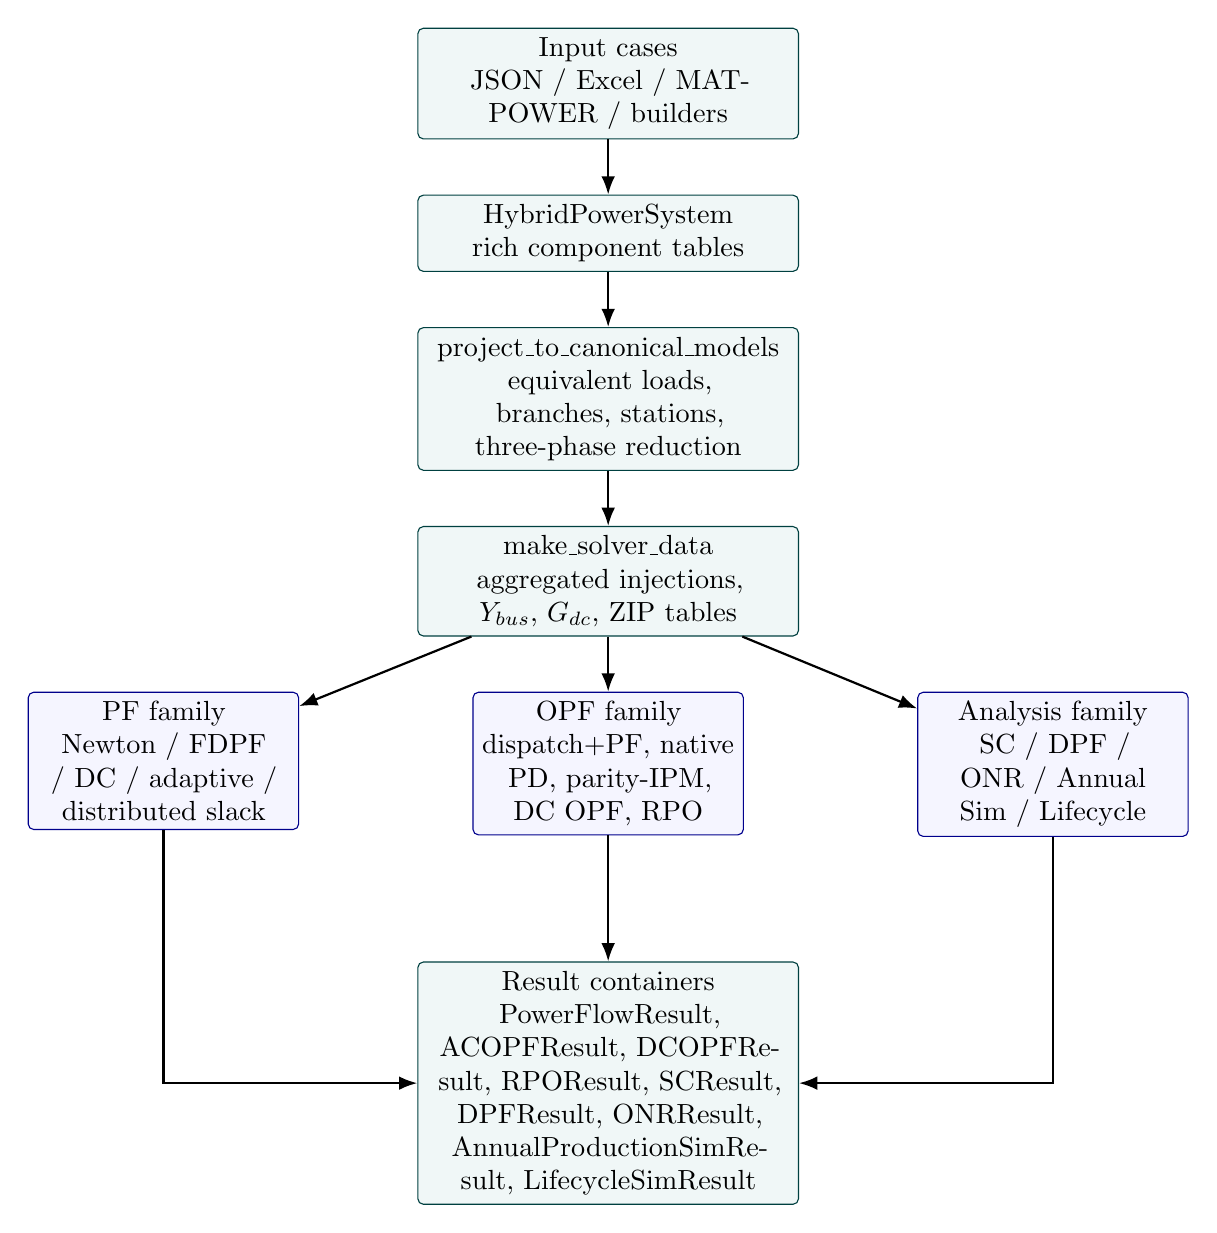
\begin{tikzpicture}[node distance=7mm and 9mm]
  \node[flowwide] (io) {Input cases\\JSON / Excel / MATPOWER / builders};
  \node[flowwide, below=of io] (model) {\texttt{HybridPowerSystem}\\rich component tables};
  \node[flowwide, below=of model] (proj) {\texttt{project\_to\_canonical\_models}\\equivalent loads, branches, stations, three-phase reduction};
  \node[flowwide, below=of proj] (solverdata) {\texttt{make\_solver\_data}\\aggregated injections, \(Y_{bus}\), \(G_{dc}\), ZIP tables};
  \node[flowbox, below left=of solverdata, xshift=-6mm] (pf) {PF family\\Newton / FDPF / DC / adaptive / distributed slack};
  \node[flowbox, below=of solverdata] (opf) {OPF family\\dispatch+PF, native PD, parity-IPM, DC OPF, RPO};
  \node[flowbox, below right=of solverdata, xshift=6mm] (analysis) {Analysis family\\SC / DPF / ONR / Annual Sim / Lifecycle};
  \node[flowwide, below=16mm of opf] (results) {Result containers\\\texttt{PowerFlowResult}, \texttt{ACOPFResult}, \texttt{DCOPFResult}, \texttt{RPOResult}, \texttt{SCResult}, \texttt{DPFResult}, \texttt{ONRResult}, \texttt{AnnualProductionSimResult}, \texttt{LifecycleSimResult}};

  \draw[flowline] (io) -- (model);
  \draw[flowline] (model) -- (proj);
  \draw[flowline] (proj) -- (solverdata);
  \draw[flowline] (solverdata) -- (pf);
  \draw[flowline] (solverdata) -- (opf);
  \draw[flowline] (solverdata) -- (analysis);
  \draw[flowline] (pf) |- (results);
  \draw[flowline] (opf) -- (results);
  \draw[flowline] (analysis) |- (results);
\end{tikzpicture}
\caption{Primary runtime data path in the current C++ module.}
\end{figure}

\subsection{Public API Surface}

The public API layer exposes a deliberately small set of top-level entry points.
The most important ones are:
\begin{itemize}
  \item \texttt{solve\_power\_flow}, \texttt{solve\_dc\_power\_flow}, \texttt{solve\_power\_flow\_fdpf},
  \item \texttt{solve\_power\_flow\_adaptive}, \texttt{solve\_power\_flow\_distributed\_slack},
  \item \texttt{solve\_ac\_dc\_power\_flow},
  \item \texttt{opf::solve\_ac\_opf},
  \item \texttt{opf::solve\_dc\_opf}, \texttt{opf::solve\_reactive\_power\_opt},
  \item \texttt{analysis::solve\_annual\_production\_simulation}, \texttt{analysis::run\_lifecycle\_simulation},
  \item solver-handle creation/reset/destruction functions for repeated PF runs on cached matrix structure.
\end{itemize}

\subsection{Solver Families and Backends}

\begin{longtable}{L{0.17\linewidth}L{0.24\linewidth}L{0.23\linewidth}L{0.26\linewidth}}
\toprule
Subsystem & Native numerical kernel & Optional backend or wrapper & Current use in module \\
\midrule
\endhead
AC/DC Newton PF & sparse linear solve through \texttt{engine::}\allowbreak\texttt{SparseLinearSolver} & Eigen SparseLU by default; UMFPACK/KLU through SuiteSparse when available & Main PF path, adaptive PF, solver-handle reuse. \\
DC PF & dense Jacobian + Eigen \texttt{FullPivLU} & none & Small-to-medium DC subnetworks. \\
FDPF & decoupled sparse LU of \(B'\) and \(B''\) & Eigen SparseLU & Fast AC approximation when the full Newton path is unnecessary. \\
Native AC OPF & custom reduced-space primal-dual KKT assembly & same sparse linear-solver abstraction as Newton PF & Used when \texttt{enable\_primal\_dual=true} and \texttt{use\_parity\_ipm=false}. \\
Parity OPF & full parity formulation plus dedicated primal-dual IPM & dense or sparse KKT solves inside parity IPM implementation & Used when \texttt{enable\_primal\_dual=true} and \texttt{use\_parity\_ipm=true}. \\
LP / MILP engine & dual simplex and native branch-and-cut & HiGHS / Gurobi adapters available through \texttt{engine::}\allowbreak\texttt{SolverAdapter} & ONR uses the native MILP branch-and-cut path. \\
NLP / MINLP engine & native IPM and branch-and-cut & IPOPT / SCIP adapters available through \texttt{engine::}\allowbreak\texttt{SolverAdapter} & Infrastructure exists, but PF/OPF modules mostly use the native paths directly. \\
DC OPF & B-$\theta$ LP/QP via \texttt{NativeQP}, \texttt{LCQP} solver, or \texttt{DualSimplex} & HiGHS / Gurobi through adapter & Used by \texttt{opf::solve\_dc\_opf}; extracts LMP from dual variables. \\
RPO (Reactive Power Optimisation) & 4-phase outer-approximation MINLP over discrete taps and switchable shunts & none (self-contained) & Used by \texttt{opf::solve\_reactive\_power\_opt}; iterates until OA gap converges. \\
LCQP (Linear/Convex QP) & Mehrotra predictor-corrector IPM with symbolic factorisation caching & none & Back-end for DC OPF (NativeQP mode) and reusable for other QP sub-problems. \\
Annual Production Sim & Hierarchical L0/L2/L3 decomposition orchestrating LP (L0) and MILP (L2/L3 via UC) & Same MILP adapters as UC (Gurobi $\to$ HiGHS $\to$ Native) & Used by \texttt{analysis::solve\_annual\_production\_simulation}. \\
Lifecycle Simulation & Multi-year loop calling annual production sim with degradation and stratified sampling & uses annual sim solvers internally & Used by \texttt{analysis::run\_lifecycle\_simulation}; produces per-year and NPV metrics. \\
\bottomrule
\end{longtable}

\subsection{Current Architectural Strengths}

\begin{itemize}
  \item The \texttt{model} layer is richer than the steady-state kernels, which makes future expansion possible without redesigning the external data model.
  \item The \texttt{project\_to\_canonical\_models} step gives PF, OPF, and SC a common data contract.
  \item The engine layer isolates linear algebra and mathematical-programming infrastructure from application modules.
  \item The compatibility namespaces \texttt{core} and \texttt{solver} reduce migration cost for older code.
\end{itemize}

\subsection{Current Architectural Friction Points}

\begin{itemize}
  \item Canonical projection is now reused by DPF and ONR as well, but the repository still lacks explicit regression tests and durable consumer keys proving that projected and non-projected views remain equivalent.
  \item The parity OPF path already fills advanced in-memory dispatch vectors, but JSON / Excel result export still exposes only the older core subset.
  \item The detailed IEC short-circuit path is now executable, but the public result contract still carries legacy scaffold fields and does not yet expose an explicit external-grid contribution bucket.
  \item Public documentation must track both canonical namespaces and their compatibility aliases, which increases cognitive load for maintainers.
\end{itemize}

\section{Engine Solver System}
\label{sec:engine-solver-system}

This section documents the solver infrastructure under
\texttt{include/hacdcpf/engine} and \texttt{src/engine} as a coherent system.
The goal is to separate three concerns that are easy to blur when reading the
repository file-by-file:
\begin{itemize}
  \item the \emph{canonical mathematical problem forms} that every backend sees,
  \item the \emph{adapter and registry layer} that dispatches a problem to a solver,
  \item the \emph{actual kernels} that are fully implemented today versus declared extension points.
\end{itemize}

This chapter is intentionally code-aligned.  When a header advertises a solver
family but the current source file is only a placeholder, the notebook states
that explicitly instead of describing the ideal future design.

\subsection{Layering Inside \texttt{hacdcpf::engine}}

The engine layer is organized in five contracts.
\begin{enumerate}
  \item \textbf{Canonical problem layer:} \texttt{problem\_types.hpp} defines the shared mathematical models such as \texttt{LPModel}, \texttt{QPModel}, and \texttt{MIPModel}.
  \item \textbf{Validation layer:} \texttt{problem\_validation.hpp/.cpp} checks structural consistency before the numerical solve begins.
  \item \textbf{Adapter layer:} \texttt{solver\_adapter.hpp} defines the uniform interface \texttt{solve\_lp}, \texttt{solve\_nlp}, \texttt{solve\_milp}, and so on.
  \item \textbf{Registry layer:} \texttt{adapter\_registry.hpp/.cpp} stores candidate adapters and selects one by supported \texttt{ProblemClass} or by name.
  \item \textbf{Kernel layer:} concrete native and external implementations live in files such as \texttt{dual\_simplex.cpp}, \texttt{lcqp\_solver.cpp}, \texttt{pdlp\_solver.cpp}, and \texttt{external\_adapters.cpp}.
\end{enumerate}

Two different solve paths coexist inside this layer:
\begin{itemize}
  \item \textbf{Canonical optimization path:} a caller builds a \texttt{ProblemClass} object and dispatches it through a \texttt{SolverAdapter}.
  \item \textbf{Direct application kernel path:} some modules call engine kernels directly without going through the adapter abstraction.  The most important example is \texttt{NewtonSolver}, which consumes \texttt{powerflow::SolverData} rather than \texttt{NonlinearSystem}.
\end{itemize}

\subsection{Canonical Problem Classes and Standard Forms}

Table~\ref{tab:engine-problem-classes} is the central contract of the engine.
Every solver family either consumes one of these objects directly or wraps a
domain-specific model into one of these forms first.

\begin{longtable}{L{0.10\linewidth}L{0.17\linewidth}L{0.37\linewidth}L{0.26\linewidth}}
\toprule
Class & C++ struct & Standard mathematical form & Current engine role \\
\midrule
\endhead
\texttt{LE} & \texttt{SparseLinSys} & Solve
\(A x = b\). & Small reusable sparse linear-system abstraction used by \texttt{NativeLinearAdapter}. \\
\texttt{NLE} & \texttt{NonlinearSystem} & Find
\(F(x)=0\), with residual and Jacobian callbacks and optional projection. & Generic Newton-style nonlinear equation interface. \\
\texttt{LP} & \texttt{LPModel} &
\(\begin{aligned}
\min/\max \quad & c^\top x \\
\text{s.t.}\quad & A x \le b, \\
& A_{eq} x = b_{eq}, \\
& \ell \le x \le u
\end{aligned}\)
& Core relaxation form for simplex, IPM-LP, PDLP, HiGHS, and Gurobi. \\
\texttt{QP} & \texttt{QPModel} &
\(\begin{aligned}
\min/\max \quad & \tfrac12 x^\top Q x + c^\top x \\
\text{s.t.}\quad & A x \le b, \\
& A_{eq} x = b_{eq}, \\
& \ell \le x \le u
\end{aligned}\)
& Convex LCQP interface for native QP IPM and Gurobi. \\
\texttt{NLP} & \texttt{NLPModel} &
\(\begin{aligned}
\min/\max \quad & f(x) \\
\text{s.t.}\quad & g(x)=0, \\
& h(x) \le 0, \\
& \ell \le x \le u
\end{aligned}\)
& Generic nonlinear optimization contract with callback and optional symbolic forms. \\
\texttt{MILP} & \texttt{MIPModel} & LP plus
\(x_j \in \mathbb{Z}\) or \(x_j \in \{0,1\}\). & Native branch-and-cut input and external MILP adapter input. \\
\texttt{MINLP} & \texttt{MINLPModel} & NLP plus integer restrictions. & Native spatial B\&B shell and SCIP-facing model form. \\
\bottomrule
\caption{Canonical problem classes in the engine layer.}
\label{tab:engine-problem-classes}
\end{longtable}

The canonical model metadata are deliberately richer than just matrices and
vectors.
\begin{itemize}
  \item \texttt{VariableMeta} attaches type, lower bound, upper bound, and name to each decision variable.
  \item \texttt{SymExpr} and \texttt{SymbolicConstraint} allow an NLP to expose a symbolic representation when an external solver prefers exported algebra over callback-only evaluation.
  \item \texttt{MIPModel} carries integer index sets, an optional warm start, unit-commitment structure hints, and branching priorities, because the branch-and-cut engine uses all of them operationally.
\end{itemize}

\subsection{Validation and Dispatch Workflow}

The adapter path is intentionally thin.  Validation and numerical work are kept
separate so that front-end modules can fail early on malformed dimensions or
invalid bounds before any solver-specific data structure is allocated.

\paragraph{Algorithm E1: Canonical Adapter Dispatch}
\begin{algorithmic}[1]
\Procedure{\texttt{dispatch\_problem}}{$cls, model, registry, preferred$}
  \State $report \gets \texttt{validate}(model)$
  \If{$report.valid = \textbf{false}$}
    \State \Return unsuccessful result with validation errors
  \EndIf
  \If{$preferred \neq \emptyset$}
    \State $adapter \gets \texttt{registry.find\_by\_name}(preferred)$
  \Else
    \State $adapter \gets \texttt{registry.first\_for}(cls)$
  \EndIf
  \If{$adapter = \varnothing$}
    \State \Return unsuccessful result with ``no adapter available''
  \EndIf
  \State Dispatch to the type-specific entry point
  \Statex \quad \texttt{solve\_le}, \texttt{solve\_nle}, \texttt{solve\_lp}, \texttt{solve\_qp}, \texttt{solve\_nlp}, \texttt{solve\_milp}, or \texttt{solve\_minlp}
  \State \Return \texttt{SolveResult}
\EndProcedure
\end{algorithmic}

At the code level, the division of responsibility is straightforward.
\begin{itemize}
  \item \texttt{SolverAdapter} provides default ``unsupported problem class'' results.
  \item Each concrete adapter overrides only the methods it really supports.
  \item \texttt{AdapterRegistry} is just an ordered list.  Selection is therefore deterministic: the first supporting adapter wins unless the caller explicitly asks for one by name.
\end{itemize}

This simple registry design is important for application code such as market
simulation and time-series PF, which register Gurobi first, HiGHS second, and a
tuned native fallback last.

\subsection{Solver Inventory and Current Implementation Status}

Table~\ref{tab:engine-solver-inventory} separates the solver \emph{interfaces}
from the solver \emph{implementations}.  This is the part most likely to reduce
maintainer confusion, because the engine now contains both fully operational
solvers and placeholder interfaces meant for future completion.

\begin{longtable}{L{0.22\linewidth}L{0.15\linewidth}L{0.20\linewidth}L{0.33\linewidth}}
\toprule
Solver family & Main class or entry point & Problem class & Current status in source \\
\midrule
\endhead
PF Newton kernel & \texttt{NewtonSolver} & direct \texttt{SolverData} path & Fully implemented power-flow-specific Newton kernel with Jacobian-pattern caching, sparse factorization reuse, line search, and bus-type switching. \\
Generic linear solve & \texttt{NativeLinearAdapter} & \texttt{LE} & Fully implemented thin wrapper over the sparse linear solver abstraction. \\
Generic NLE solve & \texttt{NativeNewtonAdapter} & \texttt{NLE} & Fully implemented regularized Newton method with backtracking. \\
Generic NLP solve & \texttt{NativeNLPAdapter} & \texttt{NLP} & Fully implemented penalty-based line-search method using callback gradients and Hessians. \\
Native NLP IPM interface & \texttt{NativeIPMAdapter} & \texttt{NLP} & Fully implemented sparse primal-dual predictor-corrector IPM with reusable KKT factorizations, shared reduced-KKT Schur solves for small equality blocks, sparse secant or finite-difference Hessian recovery when \texttt{hess} is absent, startup curvature caching across repeated solves, and IPOPT fallback for unrecovered failures. \\
Convex QP / LCQP & \texttt{NativeLCQPAdapter} & \texttt{QP}, \texttt{LP} & Fully implemented Mehrotra-style primal-dual IPM for convex QP and LP special cases. \\
High-performance LP IPM & \texttt{NativeIPMLPAdapter} & \texttt{LP} & Fully implemented predictor-corrector IPM with scaling, correctors, cached node solves, and optional crossover support. \\
Dual simplex & \texttt{solve\_lp\_with\_basis} & \texttt{LP} & Fully implemented bounded-form simplex with standard-form conversion, warm starts, sparse basis reuse, and dual-simplex reoptimization. \\
PDLP / PDHG & \texttt{NativePDLPAdapter} & \texttt{LP} & Fully implemented first-order LP solver for large sparse problems. \\
MILP / MINLP tree search & \texttt{solve\_milp\_bc}, \texttt{solve\_minlp\_bc}, \texttt{NativeBranchAndCutAdapter} & \texttt{MILP}, \texttt{MINLP} & MILP branch-and-cut is fully implemented and mature.  The MINLP path now uses the native NLP relaxation, carries multiplier-informed branch scores into child nodes, and remains backed by SCIP/IPOPT-style external fallbacks where available. \\
HiGHS wrapper & \texttt{HighsAdapter} & \texttt{LP}, \texttt{MILP} & Fully implemented external file-based wrapper around the HiGHS executable. \\
IPOPT wrapper & \texttt{IpoptAdapter} & \texttt{NLP} & Available when IPOPT is built in.  Used for external NLP backend selection. \\
SCIP wrapper & \texttt{ScipAdapter} & \texttt{MINLP} & Available when SCIP support is built in. \\
Gurobi wrapper & \texttt{GurobiAdapter} & \texttt{LP}, \texttt{QP}, \texttt{MILP} & Native C-API wrapper for high-end LP/QP/MILP solves. \\
\bottomrule
\caption{Engine solver inventory and actual implementation status.}
\label{tab:engine-solver-inventory}
\end{longtable}

\paragraph{A practical consequence for readers of the code}
When the repository mentions a ``native IPM'' for NLP, that phrase must be read
carefully.  The engine contains:
\begin{itemize}
  \item a working native IPM for \textbf{LP} in \texttt{ipm\_lp\_solver.cpp},
  \item a working native IPM for \textbf{convex QP} in \texttt{lcqp\_solver.cpp},
  \item a working native IPM for \textbf{general NLP} in \texttt{ipm\_solver.cpp}, with reduced-KKT and missing-Hessian recovery paths,
  \item and a separate working \texttt{NativeNLPAdapter} that is not a barrier IPM, but a penalty-and-line-search Newton-type method.
\end{itemize}

\paragraph{Current performance status}
The most relevant benchmark result is now the structured sparse chain NLP in
\texttt{benchmark/nlp\_ipm\_benchmark.cpp}.  On the current implementation,
the exact-Hessian native path beats IPOPT on all benchmarked sizes

\[
\text{Native/IPOPT time ratio} = 0.419\ (n=64),\quad 0.518\ (n=128),\quad 0.773\ (n=256),
\]

while the missing-Hessian path is now also faster than IPOPT across the same
benchmark family.  After the sparse secant plus finite-difference Hessian
recovery pass, shared reduced-KKT solves, and startup curvature caching, the
native missing-Hessian solve achieves

\[
\text{Native/IPOPT time ratio} = 0.340\ (n=64),\quad 0.444\ (n=128),\quad 0.677\ (n=256).
\]

So the main nonlinear performance story has changed materially: the engine is
no longer merely ``equipped with a native NLP IPM,'' but already ahead of the
external IPOPT baseline on this structured sparse benchmark in both the
exact-Hessian and missing-Hessian regimes.  The remaining engineering work is
therefore about broadening that win across more difficult NLP families, not
about filling a missing core implementation.

\subsection{Key Algorithm Workflows}

\subsubsection{Power-Flow-Specific Newton Kernel}

\texttt{NewtonSolver} is the main reusable PF engine kernel rather than a
generic optimization adapter.  It operates on \texttt{powerflow::SolverData},
builds a Jacobian context from AC/DC bus states and converter modes, and then
reuses sparse-pattern analysis aggressively across repeated solves.

\paragraph{Algorithm E2: \texttt{NewtonSolver.solve}}
\begin{algorithmic}[1]
\Procedure{\texttt{NewtonSolver.solve}}{$data, opt, init$}
  \State Initialize voltage magnitudes, angles, DC voltages, and control states
  \State Detect AC slack bus and one DC slack bus per DC island
  \State Build Jacobian context from current bus types and converter modes
  \If{cached Jacobian pattern matches \texttt{data} structure and context layout}
    \State Reuse analyzed sparse pattern and linear solver object
  \Else
    \State Rebuild Jacobian sparsity pattern and analyze it once
  \EndIf
  \For{outer PV/PQ or converter-mode adjustment loop}
    \For{$iter = 1$ to \texttt{max\_iter}}
      \State Evaluate mismatch vector and Jacobian
      \If{residual norm is below tolerance}
        \State Assemble final PF result and return
      \EndIf
      \State Factorize Jacobian, solve for Newton step, and clip step components
      \State Run globalization / backtracking line search
      \State Apply PV/PQ switching and converter control-mode updates when enabled
    \EndFor
  \EndFor
  \State Return non-converged result with profiling counters
\EndProcedure
\end{algorithmic}

\subsubsection{Generic Nonlinear Equation Solver}

\paragraph{Algorithm E3: \texttt{NativeNewtonAdapter.solve\_nle}}
\begin{algorithmic}[1]
\Procedure{\texttt{solve\_nle}}{$F(x), J(x), x_0$}
  \State Validate dimensions and callbacks
  \State $x \gets x_0$
  \For{$iter = 1$ to \texttt{max\_iter}}
    \State Evaluate residual $f \gets F(x)$
    \If{$\lVert f \rVert_\infty \le \epsilon$}
      \State Return converged result
    \EndIf
    \State Form Jacobian $J(x)$
    \For{a small regularization ladder $\lambda$}
      \State Solve \((J + \lambda I) \Delta x = -f\)
      \State Try backtracking steps $x + \alpha \Delta x$
      \If{a trial decreases residual norm}
        \State Accept step and continue outer loop
      \EndIf
    \EndFor
    \If{no acceptable step exists}
      \State Return failure: line search failed
    \EndIf
  \EndFor
  \State Return failure: maximum iterations reached
\EndProcedure
\end{algorithmic}

\subsubsection{Generic NLP Solver Used Today}

\paragraph{Algorithm E4: \texttt{NativeNLPAdapter.solve\_nlp}}
\begin{algorithmic}[1]
\Procedure{\texttt{solve\_nlp}}{$f, \nabla f, \nabla^2 f, g, h, x_0$}
  \State Validate callbacks and project $x_0$ into variable bounds
  \For{$iter = 1$ to \texttt{max\_iter}}
    \State Evaluate objective, gradient, and optional Hessian
    \State Evaluate equality and inequality violations
    \State Build penalized merit model
    \Statex \quad $\phi(x)=f(x)+\tfrac{\rho}{2}\lVert g(x) \rVert_2^2+\tfrac{\rho}{2}\lVert \max(h(x),0) \rVert_2^2$
    \State Form penalized gradient and Hessian approximation
    \If{stationarity and feasibility are small enough}
      \State Return converged result
    \EndIf
    \State Regularize Hessian and solve for a step \(\Delta x\)
    \State Run backtracking on the penalized merit function
    \State Project trial point into variable bounds
    \If{no acceptable trial point exists}
      \State Return failure
    \EndIf
  \EndFor
  \State Return best iterate with status \texttt{Max iterations reached}
\EndProcedure
\end{algorithmic}

\subsubsection{Convex QP and LCQP Solver}

\paragraph{Algorithm E5: \texttt{NativeLCQPAdapter.solve\_qp}}
\begin{algorithmic}[1]
\Procedure{\texttt{solve\_lcqp}}{$Q, c, A_{eq}, b_{eq}, \ell, u$}
  \State Apply scaling to variables, equalities, costs, and bounds
  \State Initialize primal variables at the center of finite bounds
  \State Initialize lower/upper slacks and dual multipliers to positive values
  \State Build the KKT sparsity pattern once and analyze it symbolically
  \For{$iter = 1$ to \texttt{effective\_max\_iter}}
    \State Compute stationarity, equality, slack, and complementarity residuals
    \State Compute \(\mu\) from slack-dual products
    \If{primal feasibility, dual feasibility, and gap are below tolerance}
      \State Unscale solution and return
    \EndIf
    \State Update only the diagonal-dependent part of the KKT matrix
    \State Factorize KKT numerically
    \State Choose centering parameter \(\sigma\)
    \State Solve KKT system for primal, dual, slack, and multiplier directions
    \State Compute fraction-to-boundary step sizes
    \State Update primal and dual variables
  \EndFor
  \State Return last iterate with non-converged status
\EndProcedure
\end{algorithmic}

\subsubsection{High-Performance LP Interior-Point Method}

\paragraph{Algorithm E6: \texttt{NativeIPMLPAdapter.solve\_lp}}
\begin{algorithmic}[1]
\Procedure{\texttt{solve\_ipm\_lp}}{$LP$}
  \State Convert the LP to the engine's merged internal form with box bounds, equality rows, and slack variables
  \State Optionally presolve, scale, and cache repeated node-solve data structures
  \State Initialize primal variables, slacks, and duals strictly inside the feasible box
  \For{$iter = 1$ to \texttt{max\_iter}}
    \State Compute primal residual, dual residual, and complementarity gap
    \If{all three satisfy tolerance}
      \State Export primal solution, duals, and bound multipliers; return
    \EndIf
    \State Form diagonal barrier scaling terms and factorize normal equations
    \State Compute affine predictor direction
    \State Compute affine step lengths and predicted \(\mu_{aff}\)
    \State Choose centering parameter \(\sigma\) from the affine-gap ratio
    \If{the affine step is already nearly central}
      \State Skip expensive corrector and reuse affine direction
    \Else
      \State Form Mehrotra corrector right-hand side and solve corrector system
    \EndIf
    \State Apply fraction-to-boundary step sizes and update primal/dual variables
  \EndFor
  \State Return failure or best available iterate
\EndProcedure
\end{algorithmic}

This solver is the native LP workhorse for repeated bound-change problems.  The
important engineering feature is not only the Mehrotra iteration itself, but
also the \texttt{prepare\_for\_node\_solves()} and cached-node-solve path used by
branch-and-cut workers.

\subsubsection{Dual Simplex and Standard-Form Reoptimization}

\paragraph{Algorithm E7: \texttt{solve\_lp\_with\_basis}}
\begin{algorithmic}[1]
\Procedure{\texttt{solve\_dual\_simplex}}{$LP, basis\_hint$}
  \State Convert the original LP to bounded standard form
  \Statex \quad add slack, surplus, and artificial columns as needed
  \If{a valid parent basis hint exists}
    \State Rebuild basis state, reduced costs, and basic solution from the hint
    \If{dual feasible but primal infeasible}
      \State Reoptimize by dual simplex
    \ElsIf{warm start is numerically rejected and cold start is allowed}
      \State Fall back to cold-start Phase I / Phase II
    \EndIf
  \Else
    \State Build crash basis and run cold-start Phase I / Phase II simplex
  \EndIf
  \State Persist basis information for children
  \State Return primal solution, basis, reduced costs, and dual information
\EndProcedure
\end{algorithmic}

The bounded-form conversion is central to the engine architecture.  Child nodes
usually change only bounds, so the matrix structure remains fixed while the
basis and bound-shift terms are reused.

\subsubsection{First-Order PDLP Solver}

\paragraph{Algorithm E8: \texttt{NativePDLPAdapter.solve\_lp}}
\begin{algorithmic}[1]
\Procedure{\texttt{solve\_pdlp}}{$LP$}
  \State Convert the LP into a matrix-and-box form suitable for PDHG iterations
  \State Build both CSC and CSR sparse views of the matrix
  \State Apply Ruiz row/column equilibration
  \State Build Pock--Chambolle diagonal step sizes and optional IP-PMM regularization
  \State Initialize primal and dual iterates and their running averages
  \For{$iter = 1$ to \texttt{max\_iter}}
    \State Optionally extrapolate the primal iterate
    \State Update dual variables by a row-wise sparse pass and box projection
    \State Update primal variables by a column-wise sparse pass and bound projection
    \State Update ergodic averages
    \If{it is a check iteration}
      \State Evaluate primal violation, dual stationarity, and relative gap
      \State Update the best current or averaged iterate
      \State Trigger adaptive restart if progress stagnates or periodic restart fires
      \State Adapt step gain, primal weight, and PMM regularization
      \If{current or averaged iterate satisfies tolerances}
        \State Return best iterate
      \EndIf
    \EndIf
  \EndFor
  \State Unscale the best iterate and return
\EndProcedure
\end{algorithmic}

\subsubsection{Mixed-Integer Branch-and-Cut}

\paragraph{Algorithm E9: \texttt{solve\_milp\_bc}}
\begin{algorithmic}[1]
\Procedure{\texttt{solve\_milp\_bc}}{$MIP, opt$}
  \State Validate the model and run presolve / bound tightening
  \State Solve the root LP relaxation
  \State Run root cut rounds, primal heuristics, and incumbent discovery
  \If{the root solution is integral or the gap is closed}
    \State Return immediately
  \EndIf
  \If{parallel mode is enabled}
    \State Launch heterogeneous worker threads and shared queues
  \Else
    \State Start sequential best-first / depth-first / hybrid tree loop
  \EndIf
  \While{time, node, and gap limits are not hit and the node pool is not empty}
    \State Select a node and propagate local bounds
    \State Solve the node LP relaxation, preferably by simplex warm start
    \If{the node is infeasible or dominated by incumbent}
      \State Prune node
    \ElsIf{the node solution is integral}
      \State Update incumbent and global bound
    \Else
      \State Choose branching variable using pseudocost / reliability / fallback rule
      \State Create up and down children
      \State Optionally add tree cuts or conflict information
      \State Push surviving children back to the search structure
    \EndIf
  \EndWhile
  \State Return incumbent, best bound, gap, and detailed B\&C statistics
\EndProcedure
\end{algorithmic}

The full MILP machinery is larger than this summary.  The detailed cut families,
warm-start mechanics, presolve propagation, and parallel explorer design are
documented further in Section~\ref{sec:native-branch-and-cut}.

\subsubsection{External Backend Wrapper Pattern}

\paragraph{Algorithm E10: External Adapter Shell}
\begin{algorithmic}[1]
\Procedure{\texttt{solve\_external}}{$model, executable$}
  \State Validate the canonical model
  \State Export the model to an interchange format or backend API representation
  \State Launch the external solver or native C API call
  \State Parse objective, status, primal solution, and available dual data
  \State Map backend status to \texttt{SolveStats}
  \State Return \texttt{SolveResult}
\EndProcedure
\end{algorithmic}

In the current code base, HiGHS mainly follows the file-export pattern, while
Gurobi is linked through its C API.  IPOPT and SCIP are enabled only when their
build flags are available.

\subsection{Assessment Against the Self-Contained Computation-Engine Target}

Relative to the architecture goal in \texttt{ARCHITECTURE.md}, the current
engine is best described as a \emph{strong LP/MILP-centered computation engine
with reusable nonlinear interfaces}, not yet as a fully self-contained solver
stack across linear equation, nonlinear equation, MILP, and MINLP classes.

\subsubsection{Robustness Assessment}

\paragraph{Current strengths}
The framework is structurally sound in four important ways.
\begin{itemize}
  \item \textbf{Canonical contracts are clean.}  \texttt{problem\_types.hpp}, \texttt{problem\_validation.cpp}, and the adapter interface separate model definition, validation, dispatch, and numerical work in a maintainable way.
  \item \textbf{LP/MILP solve paths defend themselves well.}  The MILP path includes validation, presolve, warm starts, fallback logic, detailed statistics, and multiple root/node strategies instead of a single brittle algorithm.
  \item \textbf{PF and linear algebra kernels are reusable.}  \texttt{NewtonSolver}, sparse linear solves, and the LP/QP kernels have enough internal structure to serve as an actual computation-engine layer rather than one-off application code.
  \item \textbf{Compatibility wrappers reduce migration risk.}  The canonical home is now \texttt{hacdcpf::engine}, while older \texttt{core}/\texttt{solver} include paths still exist as shims for the rest of the code base.
\end{itemize}

\paragraph{Current risks and gaps}
Three issues materially limit the claim of a self-contained engine.
\begin{itemize}
  \item \textbf{Native MINLP is not currently complete.}  The MINLP B\&B driver calls \texttt{solve\_nlp\_relaxation()}, and that routine currently instantiates \texttt{NativeIPMAdapter}; however, \texttt{ipm\_solver.cpp} still returns ``not implemented'' for the native NLP-IPM solve.  In other words, the tree shell exists, but the native continuous relaxation underneath is incomplete.
  \item \textbf{The generic NLP path is usable but algorithmically modest.}  \texttt{NativeNLPAdapter} is a penalty-plus-line-search Newton method, not a full primal-dual barrier solver with robust filter/merit updates, restoration, or strong multiplier handling.  That is adequate for small smooth models, but it is a weaker foundation for large constrained NLP and for MINLP relaxations.
  \item \textbf{Regression protection is uneven on the hardest path.}  The type-system and adapter tests are healthy, but the branch-and-cut test target is not currently a clean safety net for the full engine because it can abort before reaching later scenarios.  That weakens confidence in day-to-day robustness of the mixed-integer core.
\end{itemize}

\subsubsection{Performance Assessment}

\paragraph{Where the engine is strong today}
The performance architecture is already credible in the LP/MILP center.
\begin{itemize}
  \item \textbf{Root LP performance is strong.}  The native LP-IPM path is heavily engineered with scaling, cached symbolic work, and node-solve preparation; internal benchmarks have shown it can outperform the native simplex root solve by a wide margin on large UC relaxations.
  \item \textbf{MILP tree engineering is real, not superficial.}  The branch-and-cut stack contains presolve, cut pools, pseudocost and reliability branching, warm-started simplex reoptimization, heuristics, and a heterogeneous parallel mode.
  \item \textbf{Sparse factorization reuse is treated as a first-class concern.}  This is visible across \texttt{newton\_solver.cpp}, \texttt{dual\_simplex.cpp}, \texttt{ipm\_lp\_solver.cpp}, and the sparse LU support files.
\end{itemize}

\paragraph{Main bottlenecks versus the target architecture}
The remaining bottlenecks are also clear.
\begin{itemize}
  \item \textbf{Large-case MILP competitiveness is still uneven.}  Internal benchmarking shows the native B\&C path can be competitive on some UC families, but on harder large cases the external commercial or dedicated MILP solvers still retain a sizable advantage, mainly from stronger tree closure and LP reoptimization throughput.
  \item \textbf{External-wrapper overhead remains in practical workflows.}  HiGHS and SCIP mainly use file export plus subprocess execution, which is fine for portability but weaker than an in-memory backend when low latency or high-frequency repeated solves are required.
  \item \textbf{Nonlinear performance headroom is large.}  Because the native NLP-IPM path is missing, the engine does not yet have a high-performance native continuous relaxation for general MINLP.  This is the main architectural hole between today's implementation and the intended computation-engine role.
\end{itemize}

\subsubsection{Readiness Summary}

For the four solver families named in the architecture document, the present
readiness is:
\begin{center}
\begin{tabular}{L{0.18\linewidth}L{0.22\linewidth}L{0.46\linewidth}}
\toprule
Family & Current readiness & Comment \\
\midrule
Linear equation & Strong & Ready as a reusable native engine kernel \\
Nonlinear equation & Strong & Newton-style solve path is available and robust for structured models \\
MILP & Strong--Moderate & Native path is mature, but still not uniformly best-in-class on large hard instances \\
MINLP & Partial & Interface and tree shell exist, but native continuous relaxation is not yet complete \\
\bottomrule
\end{tabular}
\end{center}

Therefore, the most accurate near-term roadmap is not to redesign the engine
abstraction, but to complete the missing native NLP/MINLP core under the
existing abstraction: a real NLP-IPM or SQP-quality relaxation solver, then
MINLP-specific reliability work on branching, node recovery, and regression
testing.

\subsection{Recommended Reading Order for Maintainers}

For someone trying to understand or extend the engine, the lowest-friction order
is:
\begin{enumerate}
  \item \texttt{problem\_types.hpp} and \texttt{problem\_validation.cpp},
  \item \texttt{solver\_adapter.hpp} and \texttt{adapter\_registry.cpp},
  \item \texttt{native\_adapters.cpp} to see which kernels are actually selected,
  \item one kernel family in depth: \texttt{dual\_simplex.cpp}, \texttt{ipm\_lp\_solver.cpp}, \texttt{lcqp\_solver.cpp}, or \texttt{pdlp\_solver.cpp},
  \item \texttt{branch\_and\_cut.cpp} and its helper files for mixed-integer logic,
  \item \texttt{external\_adapters.cpp} only after the canonical forms and native solve path are already clear.
\end{enumerate}

That order mirrors the architecture itself: understand the problem contracts
first, then the dispatch layer, then the heavy numerical kernels.
\section{Native NLP Interior-Point Method: Theory, Algorithm, and Current Diagnostics}
\label{sec:engine-nlp-ipm}

This section documents the nonlinear interior-point implementation under
\texttt{include/hacdcpf/engine/ipm\_solver.hpp} and
\texttt{src/engine/ipm\_solver.cpp} with a narrower goal than
Section~\ref{sec:engine-solver-system}: to explain what the native NLP IPM is
mathematically solving, how the current code actually drives the iterations,
what the present test evidence says, and which observed behaviors should be
read as signs of a real algorithmic problem rather than mere tuning noise.

The discussion is intentionally diagnostic.  The current code already contains
multiple globalization paths, scaling hooks, restoration support, exact and
inexact curvature modes, and IPOPT fallback.  A reader who only sees the class
name \texttt{NativeIPMAdapter} can therefore easily overestimate its maturity.
The notebook below separates what is theoretically intended, what is already
implemented, and what the latest large-case evidence still says is fragile.

\subsection{Standard NLP Form and Barrier KKT System}

The canonical engine nonlinear program is the \texttt{NLPModel} from
\texttt{problem\_types.hpp}:
\begin{align}
  \min_x \quad & f(x) \\
  \text{s.t.}\quad & g(x) = 0, \\
                    & h(x) \le 0, \\
                    & \ell \le x \le u.
\end{align}

The engine converts all nonlinear inequalities and finite variable bounds into
one unified inequality block.  Introducing slacks
\(s > 0\) such that
\begin{equation}
  h(x) + s = 0,
\end{equation}
and multipliers \(\lambda\) for equalities and \(\mu > 0\) for inequalities,
the barrier KKT conditions are
\begin{align}
  \nabla f(x) + J_g(x)^\top \lambda + J_h(x)^\top \mu &= 0, \\
  g(x) &= 0, \\
  h(x) + s &= 0, \\
  S \mu &= \tau e,
\end{align}
where \(S = \operatorname{diag}(s)\).

The reduced Newton system used by both the parity-specific IPM and the generic
engine IPM is based on the primal Schur complement
\begin{equation}
  W = \nabla^2_{xx} \mathcal{L}(x,\lambda,\mu)
      + J_h(x)^\top \operatorname{diag}(\mu ./ s) J_h(x),
\end{equation}
with the Lagrangian
\begin{equation}
  \mathcal{L}(x,\lambda,\mu) = f(x) + \lambda^\top g(x) + \mu^\top h(x).
\end{equation}

This identity is critical when reading the current code quality:
if the solver only uses \(\nabla^2 f\) and drops the constraint-curvature term
inside \(\nabla^2_{xx} \mathcal{L}\), then the Newton direction is formally
incorrect for nonlinear constrained problems.  The recent engine changes fixed
that part by adding an explicit
\texttt{NLPModel::lagrangian\_hess(...)} callback and by using it inside the
native solver when available.

\subsection{Current Driver Architecture in \texttt{ipm\_solver.cpp}}

The file now contains two distinct native drivers behind the same adapter.

\paragraph{1. Filter driver (current default)}
The public \texttt{IPMOptions} now expose
\texttt{Globalization::Filter} as the default mode.  In this path, the solver
first optionally scales the problem, then runs a filter line-search method in
the style of W"achter--Biegler, with optional restoration and second-order
correction logic.  If the filter path fails, it can restore feasibility and
retry; if that still fails, it falls back to the Merit-backed native path and
ultimately to IPOPT.

The important consequence is practical rather than aesthetic:
``the native NLP IPM'' is not one single algorithm anymore.  It is a driver
stack with this order:
\begin{enumerate}
  \item scaled filter IPM,
  \item restoration-driven filter retry,
  \item merit-based native IPM,
  \item IPOPT fallback.
\end{enumerate}

\paragraph{2. Merit driver (fallback native path)}
The lower part of \texttt{ipm\_solver.cpp} still contains the earlier
Mehrotra-style merit-based driver.  It has recently been upgraded with:
\begin{itemize}
  \item exact Lagrangian Hessian support,
  \item residual-aware slack and multiplier initialization,
  \item normalized residual metrics,
  \item separate primal and dual step sizes, and
  \item best-iterate restoration.
\end{itemize}

These changes materially improved the behavior on large OPF-derived NLPs, but
they did not eliminate the main robustness issue: the generic merit line search
still breaks down on large parity OPF cases before the dedicated parity solver
does.

\subsection{Curvature Sources and Hessian Policy}

The current engine supports three curvature regimes.

\paragraph{Exact Lagrangian curvature}
If \texttt{lagrangian\_hess} is provided, the solver uses the exact
\(\nabla^2_{xx}\mathcal{L}\) callback directly.  This is now the preferred path
for parity OPF and for any NLP with nonlinear constraint curvature.

\paragraph{Objective-only Hessian}
If only \texttt{hess} is present, the solver uses the objective Hessian
\(\nabla^2 f\).  This is exact only when all constraints are linear; otherwise
it is a model misspecification, not just a performance compromise.

\paragraph{Recovered curvature}
If neither callback is present, the solver constructs sparse secant and
finite-difference approximations.  This path is still operational and is well
covered by the structured sparse-chain tests, but it is not the preferred path
for physics-heavy OPF NLPs.

\subsection{Algorithmic Workflow of the Merit Driver}

The current merit path in \texttt{ipm\_solver.cpp} can be summarized as follows.

\paragraph{Algorithm E5: Merit-backed Native NLP IPM (current implementation)}
\begin{algorithmic}[1]
\Procedure{\texttt{NativeIPM.solve\_nlp\_detail}}{$prob$}
  \State Validate callbacks, dimensions, and bounds
  \State Interiorize the initial point with respect to box bounds
  \State Evaluate \(f,\nabla f,g,J_g,h,J_h\)
  \State Initialize slacks and multipliers from inequality residuals
  \State Build exact or recovered Lagrangian Hessian
  \For{$k = 0,1,\dots$ until convergence or iteration limit}
    \State Form residuals \((r_{dual}, r_{eq}, r_{ineq})\)
    \State Compute normalized primal, dual, and complementarity metrics
    \State Build reduced primal system
    \State Solve affine predictor step
    \State Compute centering target and corrector step
    \State Compute separate primal and dual fraction-to-boundary steps
    \State Try merit-based backtracking on \((x,s,\lambda,\mu)\)
    \If{acceptable trial found}
      \State Accept step and continue
    \Else
      \State Recenter barrier state or terminate with line-search failure
    \EndIf
  \EndFor
  \If{best historical iterate satisfies tolerances}
    \State Restore best iterate and report convergence
  \Else
    \State Return failure or fall back to IPOPT
  \EndIf
\EndProcedure
\end{algorithmic}

The important diagnostic point is Step 10.  The generic solver still judges
trial steps with a scalar merit decrease condition.  For large OPF NLPs this is
currently weaker than the parity-specific direct primal/dual step acceptance,
and it is the main remaining failure mode after the recent scaling and
initialization fixes.

\subsection{Algorithmic Workflow of the Filter Driver}

The filter path is theoretically stronger and architecturally more ambitious.
It adds four ingredients that the earlier merit-only solver did not have:
\begin{itemize}
  \item problem scaling,
  \item filter-based globalization instead of one scalar merit test,
  \item optional second-order correction,
  \item one-shot restoration NLP construction and retry.
\end{itemize}

In theory this is the correct direction for difficult nonconvex NLPs.  In
practice the current source still has to be read as an implementation under
active hardening rather than a finished IPOPT-equivalent engine.  The notebook
should therefore be interpreted conservatively: the filter driver is the
intended production globalization path, while the merit driver remains the most
transparent reference path for code reading and regression triage.

\subsection{What the Unit Tests Currently Prove}

The current dedicated native-IPM test coverage is concentrated in
\texttt{tests/test\_nlp\_ipm\_solver.cpp} and
\texttt{tests/test\_minlp\_native\_ipm.cpp}.  The test evidence is summarized
in Table~\ref{tab:nlp-ipm-tests}.

\begin{table}[H]
\centering
\small
\caption{Native NLP IPM tests and what they actually verify}
\label{tab:nlp-ipm-tests}
\begin{tabularx}{\linewidth}{L{0.30\linewidth}L{0.22\linewidth}L{0.38\linewidth}}
\toprule
Test file / case & Status & What it proves \\
\midrule
\texttt{test\_nlp\_ipm\_solver}: small constrained quadratic & Passing & Basic correctness of the primal-dual solve path, multiplier output, and convergence on a smooth small NLP. \\
\texttt{test\_nlp\_ipm\_solver}: sparse chain NLP & Passing & Exact-Hessian and missing-Hessian paths both work on a structured sparse benchmark family. \\
\texttt{test\_nlp\_ipm\_solver}: exact Lagrangian Hessian callback & Passing & The solver now actually consumes \texttt{lagrangian\_hess} rather than silently dropping nonlinear constraint curvature. \\
\texttt{test\_minlp\_native\_ipm} & Passing & MINLP relaxations can call the native NLP IPM and return valid node relaxations for small cases. \\
Parity-specific Hessian finite-difference tests & Passing & The parity formulation's analytic Lagrangian Hessian matches finite-difference checks. \\
\bottomrule
\end{tabularx}
\end{table}

These tests are important but not sufficient.  They prove local algorithmic
correctness on small and structured problems; they do \emph{not} prove robust
globalization on large OPF NLPs.

\subsection{Structured Sparse Benchmark Results}

The synthetic benchmark family in
\texttt{benchmark/nlp\_ipm\_benchmark.cpp} still provides the strongest
evidence that the engine's linear algebra and Hessian handling are no longer
the main bottleneck.  On the structured sparse chain problems, the native exact
Hessian path and the missing-Hessian recovery path both solve successfully, and
the native solver remains competitive with or faster than IPOPT on this
benchmark family.

That result is still technically relevant: it means the core KKT machinery,
sparse Hessian handling, and callback contracts are not fundamentally broken.
If large OPF cases fail, the most likely culprit is now globalization and
problem scaling, not the absence of a Newton kernel.

\subsection{Large Parity-OPF Comparison Results}

The most informative recent evidence comes from the parity-OPF benchmark driver
in \texttt{tests/benchmark\_ac\_opf\_cases.cpp}, which now exposes three solve
modes on the same parity formulation:
\begin{itemize}
  \item \texttt{parity}: dedicated parity primal-dual IPM in
  \texttt{src/optimal_power_flow/parity\_ipm.cpp},
  \item \texttt{native}: generic \texttt{NativeIPMAdapter} applied to the same
  parity NLP callbacks,
  \item \texttt{ipopt}: IPOPT on the same parity NLP callbacks.
\end{itemize}

Table~\ref{tab:nlp-ipm-large-opf} summarizes the latest results after the
recent merit-driver upgrades.

\begin{table}[H]
\centering
\small
\caption{Large-case parity OPF comparison on the same NLP formulation}
\label{tab:nlp-ipm-large-opf}
\begin{tabularx}{\linewidth}{L{0.16\linewidth}L{0.13\linewidth}L{0.10\linewidth}L{0.15\linewidth}L{0.17\linewidth}L{0.19\linewidth}}
\toprule
Case & Mode & Converged & Mean time (ms) & Iterations & Status / interpretation \\
\midrule
IEEE118 & native & No & 2307.323 & 90 & \texttt{NativeIPM line search failed}; much better than the earlier 500-iteration stall, but still not robust. \\
IEEE118 & ipopt & No & 1475.001 & 500 & \texttt{Max iterations exceeded}; remains near the correct objective and near-feasible. \\
IEEE118 & parity & Yes & 15880.952 & 23 & Dedicated parity solver converges and passes PF cross-validation. \\
PEGASE2869 & native & No & 76498.973 & 33 & \texttt{NativeIPM line search failed}; materially improved over the earlier 500-iteration collapse, but still unusable as a final OPF solver. \\
PEGASE2869 & ipopt & No & 65131.865 & 500 & \texttt{Max iterations exceeded}; stays close to the parity objective. \\
PEGASE2869 & parity & Yes & 123052.538 & 61 & Dedicated parity solver converges and passes PF cross-validation. \\
\bottomrule
\end{tabularx}
\end{table}

Two conclusions follow immediately.
\begin{enumerate}
  \item The recent engine changes are real improvements: the generic native NLP
  IPM no longer simply burns the full iteration budget with catastrophic
  residuals on these OPF cases.
  \item The generic native NLP IPM is still not production-robust on large OPF
  NLPs.  The dominant failure is now a globalization failure, not missing
  curvature.
\end{enumerate}

\subsection{Current Diagnostic Interpretation: Is the Code Still Wrong?}

For code review purposes, the current answer is nuanced.

\paragraph{What is already correct enough to trust}
\begin{itemize}
  \item The engine now has a mathematically correct interface for exact
  Lagrangian Hessians.
  \item Small and structured NLP tests pass on both exact and recovered
  curvature paths.
  \item The parity formulation's Hessian and Jacobian contracts have dedicated
  finite-difference validation.
  \item The generic solver's latest upgrades improved large OPF behavior by a
  large margin compared with the earlier 500-iteration stalls.
\end{itemize}

\paragraph{What still indicates a real algorithmic problem}
The remaining large-case failures are not benign.  The following behaviors
should be read as evidence that the generic NLP IPM is still incomplete for
hard OPF-class problems:
\begin{itemize}
  \item repeated \texttt{line search failed} termination on large parity NLPs,
  \item native objective values far away from the parity and IPOPT trajectories,
  \item generic native failure on cases where the dedicated parity solver
  converges on the same formulation,
  \item dependence on fallback or parity-specific kernels for final robustness.
\end{itemize}

In other words, the code is no longer ``wrong'' in the narrow sense of missing
constraint curvature or having no native nonlinear interior-point core.
However, it is still incomplete in the stronger sense required for large-scale
OPF robustness.  The current bottleneck is algorithmic globalization rather
than Hessian formation.

\subsection{Most Likely Remaining Gap}

The recent parity-derived changes fixed the easiest-to-identify deficiencies:
better barrier-state initialization, normalized residuals, exact Lagrangian
curvature, and separate primal/dual step sizes.  The strongest remaining gap is
that the generic merit path still uses a scalar merit backtracking test, while
the dedicated parity solver accepts fraction-to-boundary primal and dual steps
more directly and augments them with OPF-specific corrector logic.

So the most likely next successful improvement path is:
\begin{enumerate}
  \item harden the filter-based driver until it reliably dominates the merit
  fallback on large OPF cases,
  \item or, alternatively, import the parity solver's direct primal/dual step
  acceptance and extra-corrector behavior more faithfully into the generic
  native path.
\end{enumerate}

For a reviewer trying to judge the present source tree, the practical summary
is simple: the native NLP IPM is now a real solver and not a placeholder, but
its robustness envelope is still substantially narrower than the dedicated
parity OPF IPM on large network NLPs.

\subsection{Reviewer-Style Risk Checklist}

For code review and regression triage, the current source can be reduced to the
following seven risk points.  These are the items most likely to explain why
the native NLP IPM still underperforms on large OPF-class problems.

\begin{enumerate}
  \item \textbf{Globalization mismatch remains the primary risk.}
  The generic native path still relies on merit or filter globalization logic
  that is materially more fragile than the direct fraction-to-boundary step
  acceptance used by the dedicated parity IPM.  Current large-case failures are
  still dominated by \texttt{line search failed} or earlier filter-stage
  rejection, not by Hessian unavailability.

  \item \textbf{Filter driver maturity is still below production level for OPF.}
  The default path in \texttt{ipm\_solver.cpp} is now the filter-based driver,
  but the current large-case evidence does not yet show that it dominates the
  merit fallback or IPOPT.  A code reviewer should therefore treat the filter
  driver as an active development path rather than as a solved final design.

  \item \textbf{The merit fallback is improved but still not robust enough.}
  The recent parity-derived upgrades fixed barrier initialization, residual
  normalization, exact Lagrangian curvature usage, separate primal and dual step
  lengths, and best-iterate restoration.  Even so, the merit path still fails
  on IEEE118 and PEGASE2869 when applied to the parity NLP callbacks.

  \item \textbf{Performance is still problem-class dependent rather than broadly solved.}
  The sparse structured chain benchmarks show that the linear algebra kernel and
  Hessian plumbing are not fundamentally broken.  However, those wins do not yet
  transfer to large nonconvex OPF NLPs.  A reviewer should therefore reject any
  blanket claim that the native NLP IPM is already competitive across realistic
  nonlinear planning workloads.

  \item \textbf{The generic solver still trails the dedicated parity solver on the same formulation.}
  This is the strongest practical red flag in the current tree.  When the same
  parity NLP callbacks are solved by \texttt{parity}, \texttt{native}, and
  \texttt{ipopt}, the dedicated parity solver converges while the generic native
  solver still fails.  That means the remaining gap is algorithmic and not just
  an interface or model-building issue.

  \item \textbf{Fallback layering can hide native weakness.}
  The current adapter stack can flow through filter solve, restoration retry,
  merit solve, and finally IPOPT fallback.  This is a useful resilience feature,
  but it also means that a superficially successful solve may not actually prove
  native robustness unless the solver path is checked explicitly.

  \item \textbf{The present bottleneck is not ``missing Hessian'' anymore.}
  That diagnosis was accurate earlier, but it is no longer the main one.  The
  more serious current risks are globalization quality, scaling fidelity, and
  parity-to-generic algorithm mismatch in difficult OPF geometries.
\end{enumerate}

In short, the present code base should be read as follows: the native NLP IPM
is algorithmically real and test-backed, but its performance and robustness are
still clearly insufficient for large OPF-class NLPs.  This is now a
globalization-and-driver-design problem more than a second-derivative problem.
\section{Generic NativeIPM vs. Parity-Specific IPM: Algorithm Gap and Refactoring Roadmap}
\label{sec:native-ipm-vs-parity-ipm}

This section isolates one question that now matters more than raw feature
completeness: why does the dedicated parity OPF interior-point solver converge
on large cases where the generic \texttt{NativeIPMAdapter} still fails on the
same nonlinear program callbacks?

The answer is no longer ``because the generic solver has no exact Hessian.''
That issue has already been addressed.  The remaining gap is that the dedicated
parity solver still has a better algorithmic envelope for OPF-class problems,
especially in globalization, centrality control, and reduced-system handling.

\subsection{What Is Actually Being Compared}

The large-case comparison in
\texttt{tests/benchmark\_ac\_opf\_cases.cpp} now evaluates three modes on the
same parity NLP model:
\begin{itemize}
  \item \texttt{parity}: the dedicated solver in \texttt{src/optimal_power_flow/parity\_ipm.cpp},
  \item \texttt{native}: the generic \texttt{NativeIPMAdapter} with the same
  callback model and exact Lagrangian Hessian,
  \item \texttt{ipopt}: IPOPT applied to the same callback model.
\end{itemize}

This matters because it removes most modeling ambiguity.  When \texttt{parity}
converges and \texttt{native} does not, the remaining explanation is mostly in
the solver algorithm, not in the OPF formulation itself.

\subsection{Algorithmic Differences}

Table~\ref{tab:native-vs-parity-ipm-gap} summarizes the most relevant current
differences.

\begin{longtable}{L{0.20\linewidth}L{0.34\linewidth}L{0.36\linewidth}}
\caption{Current algorithmic differences between generic NativeIPM and dedicated parity IPM}
\label{tab:native-vs-parity-ipm-gap}\\
\toprule
Aspect & Generic \texttt{NativeIPMAdapter} & Dedicated \texttt{parity\_ipm.cpp} \\
\midrule
\endfirsthead
\toprule
Aspect & Generic \texttt{NativeIPMAdapter} & Dedicated \texttt{parity\_ipm.cpp} \\
\midrule
\endhead
Globalization & Default path is filter-based with restoration and second-order correction; fallback path is merit-based backtracking.  In practice this stack is still fragile on large OPF NLPs. & Uses a more direct OPF-focused primal-dual step acceptance strategy with separate primal and dual fraction-to-boundary steps and no generic merit backtracking on each iteration. \\
Barrier-state initialization & Now improved with residual-aware slack and multiplier initialization in the merit path, but still embedded in a more generic driver. & Initializes slacks directly from inequality residuals to control \(\mu_i / z_i\) spread and maintain a well-conditioned condensed system from the start. \\
Residual metrics & Generic path now uses normalized residuals, but its acceptance logic still depends on a more generic merit/filter driver architecture. & Uses OPF-focused normalized convergence tests that were tuned around the parity formulation and its scaling behavior. \\
Complementarity handling & Uses a generalized predictor-corrector centering target and restoration logic. & Uses condensed complementarity handling with OPF-tested centering and direct update rules tailored to the assembled parity inequalities. \\
Extra correctors & Filter path contains second-order correction; merit path has no parity-style Gondzio block. & Includes explicit Gondzio-type extra corrector passes, which help recover centrality without relying on a merit backtracking loop. \\
Reduced Newton system & Reuses generic KKT utilities and multiple solve paths, including reduced-KKT logic for some equality patterns. & Builds and solves the condensed parity-specific Schur system directly in the exact structure expected by the OPF formulation. \\
Failure behavior on large parity OPF & Still terminates with globalization failure on IEEE118 and PEGASE2869. & Converges on IEEE118 and PEGASE2869 and passes PF cross-validation. \\
\bottomrule
\end{longtable}

\subsection{Why the Dedicated Parity Solver Still Wins}

The dedicated parity solver currently wins for three concrete reasons.

\paragraph{1. It solves the right condensed problem with less generic machinery}
The parity solver assembles the exact OPF inequality residuals, slack ratios,
and reduced Hessian contributions in one coherent path.  The generic solver can
now represent the same mathematics, but it still routes that information
through a broader abstraction that was designed to handle arbitrary NLPs rather
than one specific network structure.

\paragraph{2. Its globalization is still closer to the OPF central path}
The parity solver takes separate primal and dual fraction-to-boundary steps and
accepts them directly after corrector assembly.  The generic native solver,
especially in its merit-backed path, still has a stronger tendency to reject
steps via generic globalization rules that are mathematically sensible but too
conservative for the parity OPF trajectory.

\paragraph{3. It contains OPF-specific corrector behavior the generic solver still lacks}
The parity implementation includes Gondzio-style extra corrector passes and
best-iterate restoration in a path already tuned around parity OPF residual
geometry.  The generic solver has partially moved in this direction, but the
remaining gap is still visible on large cases.

\subsection{Current Performance Interpretation}

The present large-case evidence should be interpreted carefully.

\begin{itemize}
  \item The generic native NLP IPM is no longer catastrophically incomplete.  It
  now reaches much better neighborhoods on parity OPF than it did before the
  exact-Hessian and merit-path upgrades.
  \item However, the current performance is still not acceptable as a final OPF
  solver path.  On realistic parity cases it either fails outright or only
  approaches the correct trajectory before globalization collapses.
  \item Therefore the remaining issue is not ``can the solver form Newton
  systems?'' but rather ``can it keep and accept the right Newton trajectory on
  hard OPF landscapes?''
\end{itemize}

This is why the current Native IPM performance still looks problematic even
after recent improvements: the solver core is now mathematically much closer to
correct, but its driver logic is still not as OPF-effective as the parity
solver's dedicated update scheme.

\subsection{Implementation Backlog: PR1 / PR2 / PR3}

The next useful step is not another high-level roadmap but a concrete sequence
of pull requests.  The purpose of the following backlog is to bind the intended
algorithm changes directly to the current source functions and acceptance rules.

\paragraph{PR1: unify globalization around a direct primal/dual accepted step}

\textbf{Primary file:} \texttt{src/engine/ipm\_solver.cpp}

\textbf{Functions to change.}
\begin{itemize}
  \item \texttt{solve\_nlp\_filter\_impl}
  \item the merit fallback loop inside
  \texttt{NativeIPMAdapter::solve\_nlp\_detail}
  \item if needed, extract a shared helper for step acceptance so filter and
  merit paths do not diverge again
\end{itemize}

\textbf{What should change.}
\begin{itemize}
  \item Replace the current mixed acceptance rule in which \(x,s,\lambda\)
  are accepted by filter logic while \(\mu\) is still updated with an
  independent \texttt{alpha\_max\_dual}.  The accepted step should become one
  coherent primal-dual update decided from the same accepted trial.
  \item Introduce a direct fraction-to-boundary accepted step for the
  predictor-corrector direction before falling back to repeated generic
  backtracking.  In other words, the first-class path should be ``accept the
  Newton step if positivity and normalized residual improvement are good
  enough,'' not ``always reduce \(\alpha\) until the generic filter admits it.''
  \item Move the current acceptance decision away from pure
  \((\theta,\phi)\)-based rejection and toward a parity-style gate that checks
  positivity, normalized primal feasibility, normalized dual feasibility, and
  complementarity together.
\end{itemize}

\textbf{Acceptance criteria to replace or add.}
\begin{itemize}
  \item Replace ``accepted trial point for \(x,s,\lambda\) plus separate dual
  multiplier step'' with ``one accepted \((x,s,\lambda,\mu)\) trial.''
  \item Add an explicit rule that a full or near-full step is kept when it
  improves the normalized residual summary produced by
  \texttt{summarize\_residuals}, even if the generic filter would otherwise
  shrink it.
  \item Keep filter backtracking only as a secondary safeguard, not as the
  dominant accepted-step mechanism.
\end{itemize}

\textbf{Minimum validation.}
\begin{itemize}
  \item Re-run \texttt{benchmark\_ac\_opf\_cases} on IEEE118 and PEGASE2869 in
  \texttt{native} mode.
  \item Require that failure mode changes from early line-search collapse to a
  materially better trajectory, ideally either convergence or a much lower
  final normalized residual than the current baseline.
\end{itemize}

\paragraph{PR2: port parity-style extra correctors into the generic driver}

\textbf{Primary files:} \texttt{src/engine/ipm\_solver.cpp} and, for reference,
\texttt{src/optimal_power_flow/parity\_ipm.cpp}

\textbf{Functions to change.}
\begin{itemize}
  \item \texttt{solve\_nlp\_filter\_impl}
  \item the merit fallback loop inside
  \texttt{NativeIPMAdapter::solve\_nlp\_detail}
  \item possibly a new helper dedicated to extra-corrector assembly so the code
  does not duplicate one-off second-order logic in multiple branches
\end{itemize}

\textbf{What should change.}
\begin{itemize}
  \item Generalize the current one-shot second-order correction into a bounded
  parity-style extra-corrector loop.  The present filter path already has a
  single SOC retry; PR2 should turn that into a structured ``predictor,
  corrector, extra-corrector'' sequence.
  \item Use the extra correctors specifically to improve centrality and recover a
  larger accepted step, rather than treating them only as a feasibility patch
  after filter rejection.
  \item Ensure the extra corrector is evaluated against the same normalized
  residual summary used by the main step so that centrality improvement is
  measured rather than guessed.
\end{itemize}

\textbf{Acceptance criteria to replace or add.}
\begin{itemize}
  \item Replace ``at most one SOC attempt on first rejection'' with ``up to a
  small fixed number of extra correctors that are accepted only if residuals and
  complementarity improve.''
  \item Add an explicit centrality-improvement test based on the normalized
  complementarity and aggregate merit terms, not only on filter admissibility.
\end{itemize}

\textbf{Minimum validation.}
\begin{itemize}
  \item Re-run the same large-case parity benchmarks and compare accepted step
  lengths, iteration counts, and final residual summaries against PR1.
  \item Confirm that the generic solver is no longer losing obviously usable
  predictor-corrector steps that the parity solver would keep.
\end{itemize}

\paragraph{PR3: retune scaling, barrier-state initialization, and restoration triggers}

\textbf{Primary files:} \texttt{src/engine/ipm\_solver.cpp},
\texttt{include/hacdcpf/engine/ipm\_solver.hpp}, and any supporting scaling or
restoration helpers already used by the filter path

\textbf{Functions to change.}
\begin{itemize}
  \item \texttt{initialize\_barrier\_state}
  \item \texttt{summarize\_residuals}
  \item \texttt{solve\_nlp\_filter\_impl}
  \item restoration-trigger decisions inside the native driver stack
\end{itemize}

\textbf{What should change.}
\begin{itemize}
  \item Tighten the connection between slack initialization, multiplier
  initialization, and the normalized residual scales actually used during step
  acceptance.
  \item Revisit the current filter constants and restoration triggers so that the
  solver does not declare globalization failure too early on OPF-class problems
  that still have a promising best iterate.
  \item Make best-iterate restoration a deliberate part of the native path's
  acceptance policy rather than a final afterthought used only when the main
  loop is already exhausted.
\end{itemize}

\textbf{Acceptance criteria to replace or add.}
\begin{itemize}
  \item Replace purely absolute or mixed-scale progress decisions with
  consistently normalized criteria derived from \texttt{summarize\_residuals}.
  \item Add a restoration-entry rule based on repeated accepted-step collapse,
  not only on hard factorization or line-search failure.
  \item Keep the current best-iterate bookkeeping, but require restoration to be
  judged against parity-like feasibility and complementarity thresholds.
\end{itemize}

\textbf{Minimum validation.}
\begin{itemize}
  \item Re-run IEEE118 and PEGASE2869 in \texttt{native}, \texttt{parity}, and
  \texttt{ipopt} modes on the same callback model.
  \item Only declare the generic path ready for default use on parity OPF when
  it converges without IPOPT fallback, matches parity objective and feasibility
  closely, and no longer fails primarily through globalization breakdown.
\end{itemize}

\paragraph{Why this PR order matters}

This order is intentional.  PR1 attacks the most visible current defect, namely
that the accepted step is still too generic and internally inconsistent.  PR2
then adds the parity-style corrector machinery needed to keep that better step
on hard iterations.  PR3 only makes sense after PR1 and PR2, because scaling
and restoration thresholds cannot be tuned meaningfully while the accepted-step
logic itself is still unstable.

\subsection{Practical Bottom Line}

The current technical conclusion is blunt but useful.

\begin{itemize}
  \item The generic NativeIPM is now a genuine interior-point implementation and
  no longer a placeholder.
  \item Its current performance is still problematic on large OPF-class NLPs.
  \item The parity-specific solver remains the stronger implementation for this
  problem family.
  \item The right next move is not more Hessian plumbing, but better
  globalization and closer transfer of parity's accepted-step logic into the
  generic driver.
\end{itemize}

So if the review question is whether the current native NLP IPM still has major
performance problems, the answer is yes.  They are now concentrated in the
driver and globalization layer, not in the existence of the Newton system or
the availability of exact second derivatives.
\section{Symbols, Indexing, and Sign Convention}

\subsection{Electrical Bases}
\begin{align}
S_{base} &= \text{system apparent-power base (MVA)}, \\
V_{base} &= \text{nominal line-line voltage base (kV)}, \\
Z_{base} &= \frac{V_{base}^2}{S_{base}}, \\
I_{base} &= \frac{S_{base}}{\sqrt{3}V_{base}}.
\end{align}

\subsection{Sets and Indexing}

\begin{align}
\mathcal{N}_{ac} &:\text{ AC buses}, &
\mathcal{E}_{ac} &:\text{ AC branches}, \\
\mathcal{N}_{dc} &:\text{ DC buses}, &
\mathcal{E}_{dc} &:\text{ DC branches}, \\
\mathcal{N}_{sl} &:\text{ AC slack buses}, &
\mathcal{N}_{PQ} &:\text{ AC PQ buses}, \\
\mathcal{N}_{PV} &:\text{ AC PV buses}, &
\mathcal{N}_{sl}^{\qual{dc}} &:\text{ DC voltage-controlled buses}.
\end{align}

The public model stores external bus identifiers in each component
(\texttt{bus}, \texttt{from\_bus}, \texttt{to\_bus}).  Most solver kernels then remap
those identifiers into contiguous zero-based local indices.

\subsection{Core AC and DC State Variables}
\begin{align}
V_i &= v_i e^{j\theta_i}, \\
Y_{ij} &= G_{ij} + jB_{ij}, \\
V_k^{\qual{dc}} &= v_k^{\qual{dc}}, \\
P_k^{\qual{dc,calc}} &= v_k^{\qual{dc}}(G_{dc}v^{\qual{dc}})_k.
\end{align}

For the main Newton power-flow path, the state vector is
\begin{align}
x_{PF} = \begin{bmatrix} \theta_{\mathcal{N}_{ac}\setminus\mathcal{N}_{sl}} & v_{\mathcal{N}_{PQ}} & v^{\qual{dc}}_{\mathcal{N}_{dc}\setminus\mathcal{N}_{sl}^{\qual{dc}}} \end{bmatrix}^{\top}.
\end{align}

For the native primal-dual AC OPF path, the decision vector is extended to
include generator dispatch and converter operating points:
\begin{align}
x_{OPF} = \begin{bmatrix}
\theta & v & P_g & Q_g & v^{\qual{dc}} & P^{\qual{conv,ac}} & Q^{\qual{conv,ac}} & P^{\qual{conv,dc}}
\end{bmatrix}^{\top},
\end{align}
with additional load-shedding variables in the parity formulation.

\subsection{Unified Sign Convention: Bus Injection Positive}

The current C++ module uses one consistent notation in the PF kernels and the
notebook adopts the same rule:
\begin{quote}
\textbf{Positive active or reactive power at a bus means injection into the network from the component attached to that bus.}
\end{quote}

Loads therefore store positive demand values in their data model, but they enter
power-balance equations with a minus sign.

\begin{longtable}{L{0.24\linewidth}L{0.48\linewidth}L{0.18\linewidth}}
\toprule
Quantity / field & Positive value means & Consequence in equations \\
\midrule
\endhead
\texttt{Generator::pg\_mw}, \texttt{qg\_mvar} & generator injects active/reactive power into its AC bus & added to \(P_i^{\qual{spec}}, Q_i^{\qual{spec}}\). \\
\texttt{Load::p\_mw}, \texttt{q\_mvar} & consumption requested from the network & subtracted from \(P_i^{\qual{spec}}, Q_i^{\qual{spec}}\); ZIP dependence scales the subtraction. \\
\texttt{Storage::p\_mw} & discharge to the grid; charging is negative \(P\) & treated as generation when positive, load when negative. \\
\texttt{Microgrid::p\_exchange\_mw} & export from the microgrid to the host AC grid & added as AC-bus injection in PF; ignored when the microgrid is islanded. \\
\texttt{VSCConverter} AC-side \(P^{\qual{conv,ac}}\) & converter injects active power into the AC bus & positive AC injection must be balanced by negative DC-bus injection plus losses. \\
\texttt{VSCConverter} DC-side \(P^{\qual{conv,dc}}\) & converter injects active power into the DC bus & the current code enforces \(P^{\qual{conv,ac}}+P^{\qual{conv,dc}}+P^{\qual{loss}}=0\). \\
\texttt{DCDCConverter::p\_ref\_mw} & positive transfer from \texttt{bus\_in} toward \texttt{bus\_out} & implemented as negative injection at \texttt{bus\_in} and positive injection at \texttt{bus\_out}. \\
\texttt{BranchFlow::pf\_mw} & active power sent from \texttt{from\_bus} to \texttt{to\_bus} & reporting only; no sign reversal in stored result. \\
\bottomrule
\end{longtable}

\subsection{Power-Balance Template}

With bus-injection-positive notation, the balance equations are written as
\begin{align}
\Delta P_i &= P_i^{\qual{spec}} - P_i^{\qual{calc}}, \\
\Delta Q_i &= Q_i^{\qual{spec}} - Q_i^{\qual{calc}}, \\
\Delta P_k^{\qual{dc}} &= P_k^{\qual{dc,spec}} - P_k^{\qual{dc,calc}}.
\end{align}

The specified term is assembled by adding all component injections and then
subtracting all demand terms.  This is the convention followed by the PF
residual evaluator, the native AC OPF assembly, and the parity formulation.

\section{Information Models and Field Dictionaries}
\label{sec:components}

\subsection{Modeling Layers Used by the Code}

The code base uses three distinct model layers.
\begin{enumerate}
  \item \textbf{Public information model}: the rich structs under \texttt{include/hacdcpf/model/} used by I/O, case builders, and external callers.
  \item \textbf{Canonical steady-state model}: the projected subset generated by \texttt{project\_to\_canonical\_models}, where rich components are converted into equivalent loads, branches, or aggregated injections.
  \item \textbf{Solver assembly model}: \texttt{powerflow::SolverData}, which stores contiguous vectors, aggregated per-bus injections, ZIP coefficients, and sparse matrices needed by the PF and OPF kernels.
\end{enumerate}

\subsection{System Containers and Solver-Level Metadata}

\subsubsection*{System containers}
\begin{longtable}{L{0.20\linewidth}L{0.53\linewidth}L{0.19\linewidth}}
\toprule
Struct / group & Fields and meaning & Primary consumers \\
\midrule
\endhead
\texttt{ACSystem} & \texttt{buses}, \texttt{branches}, \texttt{generators}, \texttt{loads}, \texttt{shunts}, \texttt{storage}, \texttt{renewable\_gens}, \texttt{pv\_systems}, \texttt{transformers\_2w}, \texttt{transformers\_3w}, \texttt{switches}, \texttt{charging\_stations}, \texttt{chargers}, \texttt{external\_grids}, \texttt{motors}; plus \texttt{base\_mva}, \texttt{freq\_hz}, \texttt{name}.  It is the main AC container for PF, DPF, SC, and ONR. & PF, OPF, SC, DPF, ONR, I/O \\
\texttt{DCSystem} & \texttt{buses}, \texttt{branches}, \texttt{loads}, \texttt{storage}, \texttt{static\_generators}, plus \texttt{base\_mva} and \texttt{name}.  Used only by hybrid AC/DC solvers. & PF, OPF, I/O \\
\texttt{HybridPowerSystem} & Holds \texttt{ac}, \texttt{dc}, \texttt{vsc\_converters}, \texttt{dcdc\_converters}, \texttt{energy\_routers}, \texttt{mobile\_storage}, \texttt{vpps}, \texttt{microgrids}, optional \texttt{three\_phase\_ac}, and global \texttt{base\_mva}.  This is the top-level public object for most APIs. & all top-level APIs \\
\texttt{ThreePhaseACSystem} & Optional unbalanced AC subsystem with three-phase buses, lines, transformers, loads, generators, and external grids.  It is projected to canonical AC objects when the explicit \texttt{ACSystem} is empty. & projection, PF, SC, I/O \\
\bottomrule
\end{longtable}

\subsubsection*{Power-flow options and results}
\begin{longtable}{L{0.20\linewidth}L{0.53\linewidth}L{0.19\linewidth}}
\toprule
Struct / group & Fields and meaning & Primary consumers \\
\midrule
\endhead
\texttt{InitialState} & \texttt{vm}, \texttt{va}, \texttt{vdc} provide optional warm starts for AC magnitude, AC angle, and DC voltage states. & Newton PF, DC PF \\
\texttt{ReactiveLimit} & \texttt{qmin}, \texttt{qmax} define reactive limits used by adaptive/PV-PQ logic. & adaptive PF extensions \\
\texttt{DistributedSlack} & \texttt{participating\_buses}, \texttt{participation\_factors}, \texttt{reference\_bus}, and optional \texttt{max\_participation\_p} describe how slack mismatch is redistributed. & distributed-slack PF \\
\texttt{PowerFlowOptions} & Iteration and tolerance controls: \texttt{max\_iter}, \texttt{tol}; robustness controls: line search, regularization, and step clipping; PV/PQ and converter hysteresis parameters; ZIP weights; solver profiling flag; \texttt{loss\_model}; FDPF iteration cap. & PF family \\
\texttt{SolverProfiling} & Sparse-factorization counters, line-search and regularization statistics, PV/PQ switches, converter-mode switches, timing vectors, and cumulative timing totals. & PF result diagnostics \\
\texttt{PowerFlowResult} & Solved states \texttt{vm}, \texttt{va}, \texttt{vdc}; status fields \texttt{converged}, \texttt{iterations}, \texttt{residual}; and derived reports \texttt{branch\_flows}, \texttt{vsc\_transfers}, \texttt{dcdc\_transfers}, \texttt{er\_port\_transfers}. & PF family outputs \\
\texttt{AdaptiveSolveResult}, \texttt{IslandedSolveResult}, \texttt{DistributedSlackResult} & Variants of PF results that additionally expose detected \texttt{islands}, distributed-slack allocations, and buses hitting slack-sharing limits. & adaptive / islanded / distributed-slack PF \\
\bottomrule
\end{longtable}

\subsubsection*{Analysis and OPF options/results}
\begin{longtable}{L{0.20\linewidth}L{0.53\linewidth}L{0.19\linewidth}}
\toprule
Struct / group & Fields and meaning & Primary consumers \\
\midrule
\endhead
\texttt{ACOPFOptions} & Inner/outer iteration caps, feasibility/stationarity tolerances, barrier schedule, merit-penalty and regularization terms, line-search settings, parallel AC evaluation threads, and path-selection flags \texttt{enable\_primal\_dual}, \texttt{use\_parity\_ipm}, \texttt{allow\_fallback}. & AC OPF \\
\texttt{ACOPFResult} & Voltage solution, generator dispatch, optional bus-level load shedding, converter operating points, convergence metrics, status text, and profiling summary. & AC OPF output \\
\texttt{SCOptions}, \texttt{SCResult}, \texttt{BusFaultResult} & Short-circuit fault type, voltage correction factor, default machine reactance, per-bus Thevenin impedance, fault current, and short-circuit power. & short circuit \\
\texttt{DPFOptions}, \texttt{DPFResult} & BFS controls, optional shunt and Q-limit handling, radial PF voltages, branch powers, total losses, and residual. & distribution PF \\
\texttt{ONROptions}, \texttt{ONRResult} & Voltage bounds, thermal defaults, big-\(M\), MILP gap and time limit, resulting branch statuses, estimated loss, verification PF, and branch-and-cut diagnostics. & ONR \\
\bottomrule
\end{longtable}

\subsubsection*{\texttt{powerflow::SolverData}}
\begin{longtable}{L{0.20\linewidth}L{0.53\linewidth}L{0.19\linewidth}}
\toprule
Group & Fields and meaning & Primary consumers \\
\midrule
\endhead
Canonical component tables & Copies of projected AC/DC buses, branches, generators, converters, DCDC converters, energy routers, loads, DERs, shunts, switches, charging stations, external grids, VPPs, microgrids, and mobile storage. & PF, native OPF \\
Aggregated steady-state injections & \texttt{pg}, \texttt{qg} hold per-bus generation after aggregation of generators, static generators, renewables, PV, storage, VPPs, microgrids, and mobile storage. & PF, native OPF \\
Demand model data & \texttt{has\_component\_loads}, \texttt{pd\_pu}, \texttt{qd\_pu}, and per-bus ZIP coefficient vectors describe the demand model after load-table aggregation. & PF, native OPF \\
Network matrices & \texttt{ybus} and \texttt{gdc} store the canonical AC admittance and DC conductance matrices; \texttt{build\_id} is used to validate Jacobian-pattern caching. & PF, native OPF \\
Bookkeeping & \texttt{base\_mva}, \texttt{loss\_model}, and global ZIP weights copied from \texttt{PowerFlowOptions}. & PF, native OPF \\
\bottomrule
\end{longtable}

\subsection{Component Inventory}

Table~\ref{tab:model-inventory} enumerates the rich public models currently
present in the repository.

\begin{longtable}{L{0.23\linewidth}L{0.32\linewidth}L{0.33\linewidth}}
\caption{Public component-model inventory}\label{tab:model-inventory}\\
\toprule
Struct & Mathematical role & Current steady-state integration mode \\
\midrule
\endfirsthead
\toprule
Struct & Mathematical role & Current steady-state integration mode \\
\midrule
\endhead
\bottomrule
\endfoot
\texttt{ACBus} & AC state host, voltage limits, embedded bus demand and shunt & direct \\
\texttt{ACBranch} & AC series/shunt admittance, tap and phase-shift branch & direct \\
\texttt{Transformer2W} & named two-winding transformer with short-circuit/tap data & projected to \texttt{ACBranch} \\
\texttt{Transformer3W} & explicit three-winding transformer with pairwise short-circuit data & projected to three \texttt{ACBranch} equivalents \\
\texttt{ExternalGrid} & slack source and short-circuit source equivalent & direct in PF/SC \\
\texttt{AsynchronousMotor} & motor fault contribution & SC only \\
\texttt{Generator} & synchronous generator dispatch and limits & direct \\
\texttt{StaticGenerator} & fixed/scaled distributed generation & direct fixed injection \\
\texttt{RenewableGen} & renewable injection with curtailment metadata & direct fixed injection; OPF curtailment slot not fully wired \\
\texttt{PVSystem} & PV inverter and array metadata & direct fixed injection with power-curve helper \\
\texttt{Load} & AC demand with ZIP and motor-fraction metadata & direct \\
\texttt{FlexibleLoad} & demand-response model & projected to \texttt{Load}; direct OPF flexibility variable not yet wired \\
\texttt{AsymmetricLoad} & per-phase aggregate demand & projected to \texttt{Load} \\
\texttt{Shunt} & fixed or stepped shunt element & direct in PF; simplified treatment in DPF \\
\texttt{Switch} & switching device with electrical/protection data & projected to \texttt{ACBranch} for PF/OPF/SC \\
\texttt{ChargingStation} & aggregate EV charging demand & direct fixed load \\
\texttt{Charger} & individual EV charger & aggregated into \texttt{ChargingStation} on projection \\
\texttt{Storage} & stationary storage power and energy state & direct fixed injection in current steady-state solvers \\
\texttt{MobileStorage} & relocatable storage resource & direct fixed injection when stationary \\
\texttt{VirtualPowerPlant} & aggregated DER portfolio & direct fixed AC-bus injection \\
\texttt{Microgrid} & PCC exchange model & direct fixed AC-bus injection when grid-connected \\
\texttt{DCBus} & DC voltage host and DC demand host & direct \\
\texttt{DCBranch} & DC resistive branch & direct \\
\texttt{DCLoad} & DC active demand & direct \\
\texttt{VSCConverter} & AC/DC coupling with loss model and control mode & direct \\
\texttt{DCDCConverter} & DC/DC transfer device with efficiency and \(I^2R\) conduction loss & direct in PF and parity OPF (decision variable with Jacobian and Hessian) \\
\texttt{EnergyRouterPort} & AC or DC port injection for a multi-port router & direct fixed injection \\
\texttt{EnergyRouter} & multi-port converter container & direct through its ports \\
\texttt{ThreePhaseACBus} & optional unbalanced bus model & projected to \texttt{ACBus} \\
\texttt{ThreePhaseACLine} & optional unbalanced line model & projected to \texttt{ACBranch} using positive sequence \\
\texttt{ThreePhaseTransformer} & optional unbalanced transformer model & projected to \texttt{Transformer2W} equivalent \\
\texttt{ThreePhaseLoad} & optional unbalanced load model & projected to \texttt{Load} \\
\texttt{ThreePhaseGenerator} & optional unbalanced generator model & projected to \texttt{Generator} \\
\texttt{ThreePhaseExternalGrid} & optional unbalanced slack/grid equivalent & projected to \texttt{ExternalGrid} \\
\bottomrule
\end{longtable}

\subsection{AC Network Elements}

\subsubsection*{\texttt{ACBus}}
\begin{longtable}{L{0.20\linewidth}L{0.53\linewidth}L{0.19\linewidth}}
\toprule
Field group & Detailed explanation & Used by \\
\midrule
\endhead
Identity and topology & \texttt{index} is the external bus identifier referenced by other components; \texttt{name} is purely descriptive; \texttt{area} and \texttt{zone} are retained for partitioning and reporting. & all modules \\
Steady-state electrical state & \texttt{bus\_type}, \texttt{vm\_pu}, \texttt{va\_deg}, \texttt{base\_kv}, \texttt{vmax\_pu}, \texttt{vmin\_pu}, \texttt{in\_service}.  These fields initialize the PF state, define slack/PV/PQ behavior, and bound voltages. & PF, OPF, DPF \\
Embedded demand and shunt & \texttt{pd\_mw}, \texttt{qd\_mvar} store fallback bus demand when no load table is present; \texttt{gs\_mw}, \texttt{bs\_mvar} store bus shunt terms. & PF, OPF, DPF, ONR \\
Resilience / geography & \texttt{n\_customers}, \texttt{importance}, \texttt{latitude}, \texttt{longitude}.  These are not yet decision variables, but they are useful for planning logic, GIS, or load-priority extensions. & planning / future use \\
\bottomrule
\end{longtable}

\subsubsection*{\texttt{ACBranch}}
\begin{longtable}{L{0.20\linewidth}L{0.53\linewidth}L{0.19\linewidth}}
\toprule
Field group & Detailed explanation & Used by \\
\midrule
\endhead
Connectivity & \texttt{index}, \texttt{from\_bus}, \texttt{to\_bus}, \texttt{in\_service}, \texttt{name}.  Bus references use external bus IDs. & PF, OPF, SC, DPF, ONR \\
Positive-sequence electrical data & \texttt{r\_pu}, \texttt{x\_pu}, \texttt{b\_pu}, \texttt{tap}, \texttt{shift\_deg}.  These define the AC \(\pi\)-model and branch-flow reporting. & PF, OPF, SC, DPF, ONR \\
Ratings and physical metadata & \texttt{rate\_a\_mva}, \texttt{rate\_b\_mva}, \texttt{rate\_c\_mva}, \texttt{length\_km}.  Only \texttt{rate\_a\_mva} is used directly by the current OPF/ONR limits. & OPF, ONR, reporting \\
Reliability and sequence data & \texttt{failure\_rate}, \texttt{mttr\_hr}, \texttt{r0\_pu}, \texttt{x0\_pu}, \texttt{b0\_pu}, and transformer-nameplate fields \texttt{vn\_hv\_kv}, \texttt{vn\_lv\_kv}, \texttt{sn\_mva}.  These support SC correction factors and planning extensions. & SC, planning \\
\bottomrule
\end{longtable}

\subsubsection*{\texttt{Transformer2W}, \texttt{Transformer3W}, and \texttt{Switch}}
\begin{longtable}{L{0.20\linewidth}L{0.53\linewidth}L{0.19\linewidth}}
\toprule
Struct & Field-level explanation & Current treatment \\
\midrule
\endhead
\texttt{Transformer2W} & Identity/connectivity fields \texttt{index}, \texttt{name}, \texttt{hv\_bus}, \texttt{lv\_bus}, \texttt{in\_service}; nameplate fields \texttt{sn\_mva}, \texttt{vn\_hv\_kv}, \texttt{vn\_lv\_kv}; short-circuit fields \texttt{vk\_percent}, \texttt{vkr\_percent}, \texttt{pk\_kw}; no-load fields \texttt{pfe\_kw}, \texttt{i0\_percent}; tap-changer fields \texttt{tap\_side}, \texttt{tap\_pos}, \texttt{tap\_min}, \texttt{tap\_max}, \texttt{tap\_neutral}, \texttt{tap\_step\_percent}; phase shift \texttt{shift\_deg}; zero-sequence fields \texttt{z0\_percent}, \texttt{x0\_r0}; reliability fields \texttt{mtbf\_hours}, \texttt{mttr\_hours}. & projected to one equivalent \texttt{ACBranch} \\
\texttt{Transformer3W} & Connectivity \texttt{hv\_bus}, \texttt{mv\_bus}, \texttt{lv\_bus}; per-winding ratings \texttt{sn\_hv\_mva}, \texttt{sn\_mv\_mva}, \texttt{sn\_lv\_mva}; pairwise short-circuit data \texttt{vk\_hv\_mv\_percent}, \texttt{vk\_hv\_lv\_percent}, \texttt{vk\_mv\_lv\_percent} and the matching \texttt{vkr} fields; tap data and phase shifts \texttt{shift\_mv\_deg}, \texttt{shift\_lv\_deg}. & projected to three equivalent \texttt{ACBranch} objects \\
\texttt{Switch} & Topology fields \texttt{bus\_from}, \texttt{bus\_to}, \texttt{closed}; electrical fields \texttt{r\_contact\_ohm}, \texttt{z\_ohm}, \texttt{i\_rated\_ka}, \texttt{i\_breaking\_ka}; protection fields \texttt{element\_type}, \texttt{element\_id}; automation fields \texttt{is\_remote}, \texttt{is\_automated}, \texttt{t\_operation\_s}; reliability fields \texttt{p\_sw\_fail}, \texttt{mtbf\_hours}, \texttt{mttr\_hours}. & projected to equivalent branch with \texttt{in\_service = closed} \\
\bottomrule
\end{longtable}

\subsubsection*{\texttt{ExternalGrid} and \texttt{AsynchronousMotor}}
\begin{longtable}{L{0.20\linewidth}L{0.53\linewidth}L{0.19\linewidth}}
\toprule
Struct & Field-level explanation & Current treatment \\
\midrule
\endhead
\texttt{ExternalGrid} & \texttt{bus}, \texttt{vm\_pu}, \texttt{va\_deg} establish slack voltage targets; \texttt{s\_sc\_max\_mva}, \texttt{s\_sc\_min\_mva}, \texttt{rx\_max}, \texttt{rx\_min}, \texttt{r\_pu}, \texttt{x\_pu}, \texttt{r0\_pu}, \texttt{x0\_pu}, \texttt{vn\_kv}, \texttt{ikq\_ka}, \texttt{x\_r} store fault-source data; \texttt{controllable} can support future dispatch logic. & PF slack/source and SC source equivalent \\
\texttt{AsynchronousMotor} & \texttt{bus}, \texttt{vn\_kv}, \texttt{sn\_mva}, \texttt{r\_pu}, \texttt{x\_pu}, \texttt{x\_r}, \texttt{lrc}, \texttt{poles}, \texttt{cos\_phi}, \texttt{efficiency}, \texttt{r0\_pu}, \texttt{x0\_pu}.  These fields describe the motor contribution to short-circuit current, not a steady-state PF state. & SC only \\
\bottomrule
\end{longtable}

\subsection{Load Models and Demand-Side Components}

\begin{longtable}{L{0.20\linewidth}L{0.53\linewidth}L{0.19\linewidth}}
\toprule
Struct & Field-level explanation & Current treatment \\
\midrule
\endhead
\texttt{Load} & Identity fields \texttt{index}, \texttt{bus}, \texttt{name}, \texttt{in\_service}; steady-state demand \texttt{p\_mw}, \texttt{q\_mvar}; model selector \texttt{model}; ZIP coefficients \texttt{z\_percent\_p}, \texttt{i\_percent\_p}, \texttt{p\_percent\_p}, and the matching \texttt{q} fields; demand-response metadata \texttt{controllable}, \texttt{p\_min\_mw}, \texttt{cost\_mw}; load-priority metadata \texttt{priority}, \texttt{n\_customers}, \texttt{profile\_id}; motor-fraction SC metadata \texttt{sn\_mva}, \texttt{motor\_percent}, \texttt{x\_sub\_pu}, \texttt{r\_sc\_pu}. & direct in PF/OPF/SC \\
\texttt{FlexibleLoad} & Baseline demand \texttt{p\_mw}, \texttt{q\_mvar}; flexibility envelope \texttt{flex\_up\_mw}, \texttt{flex\_down\_mw}, \texttt{flex\_duration\_h}; response timing \texttt{response\_time\_s}, \texttt{ramp\_rate\_mw\_min}, \texttt{availability\_pct}; \texttt{control\_area}. & projected to equivalent \texttt{Load}; direct OPF flexibility variable not yet active \\
\texttt{AsymmetricLoad} & Per-phase rated values \texttt{pa\_rated\_mw}, \dots, \texttt{qc\_rated\_mvar}; per-phase actual values \texttt{pa\_mw}, \dots, \texttt{qc\_mvar}; \texttt{connection}, \texttt{grounded}, \texttt{scaling}; ZIP shares \texttt{const\_z\_percent}, \texttt{const\_i\_percent}, \texttt{const\_p\_percent}. & projected to aggregated \texttt{Load} \\
\texttt{DCLoad} & \texttt{p\_mw} is the direct active demand at a DC bus; \texttt{controllable}, \texttt{p\_min\_mw}, \texttt{cost\_mw}, and \texttt{profile\_id} are control metadata for future extensions. & direct in DC PF and hybrid OPF balances \\
\texttt{ChargingStation} & \texttt{bus}, \texttt{n\_fast}, \texttt{n\_slow}, \texttt{num\_chargers}; capacity fields \texttt{p\_fast\_max\_kw}, \texttt{p\_slow\_max\_kw}, \texttt{max\_power\_kw}; utilization fields \texttt{simultaneity\_factor}, \texttt{power\_factor}, \texttt{utilization\_rate}; aggregated operating demand \texttt{p\_total\_kw}, \texttt{q\_total\_kvar}. & direct fixed load \\
\texttt{Charger} & \texttt{station\_id} links the charger to its parent station; \texttt{charger\_type}, \texttt{p\_rated\_kw}, \texttt{p\_ch\_max\_kw}, \texttt{p\_ch\_min\_kw}, \texttt{eta}, \texttt{v2g\_capable}, \texttt{p\_dis\_max\_kw}. & aggregated into \texttt{ChargingStation} during projection \\
\bottomrule
\end{longtable}

\subsection{Generation, Storage, and Aggregation Components}

\begin{longtable}{L{0.20\linewidth}L{0.53\linewidth}L{0.19\linewidth}}
\toprule
Struct & Field-level explanation & Current treatment \\
\midrule
\endhead
\texttt{Generator} & Dispatch/state fields \texttt{pg\_mw}, \texttt{qg\_mvar}, \texttt{vg\_pu}, \texttt{is\_slack}; limits \texttt{pmax\_mw}, \texttt{pmin\_mw}, \texttt{qmax\_mvar}, \texttt{qmin\_mvar}; quadratic cost coefficients \texttt{cost\_c2}, \texttt{cost\_c1}, \texttt{cost\_c0}; unit-commitment metadata \texttt{startup\_cost}, \texttt{shutdown\_cost}, \texttt{min\_up\_time\_hr}, \texttt{min\_dn\_time\_hr}, \texttt{ramp\_up\_mw\_min}, \texttt{ramp\_dn\_mw\_min}; machine/stability data \texttt{mbase\_mva}, \texttt{inertia\_h}, \texttt{droop\_r}, \texttt{xd\_pu}, \texttt{xdp\_pu}, \texttt{xdpp\_pu}, \texttt{td0p\_s}, \texttt{td0pp\_s}; SC and environmental metadata \texttt{ra\_pu}, \texttt{vn\_kv}, \texttt{cos\_phi}, \texttt{xq\_pu}, \texttt{xd\_xq}, \texttt{x0\_pu}, \texttt{r0\_pu}, emission factors, outage rate, and repair time. & direct \\
\texttt{StaticGenerator} & Fixed or scaled DER injection \texttt{p\_mw}, \texttt{q\_mvar}, \texttt{scaling}; device rating/limits \texttt{p\_rated\_mw}, \texttt{sn\_mva}, \texttt{pmax\_mw}, \texttt{pmin\_mw}, \texttt{qmax\_mvar}, \texttt{qmin\_mvar}; control metadata \texttt{controllable}, \texttt{v\_ref\_pu}, \texttt{k\_p}, \texttt{k\_q}; SC metadata \texttt{k}, \texttt{rx}. & direct fixed injection \\
\texttt{RenewableGen} & \texttt{type}, actual output \texttt{p\_mw}, \texttt{q\_mvar}, rated power \texttt{p\_rated\_mw}, reactive limits, curtailability flag, curtailment cost, capacity factor, profile pointer, and avoided-emission factor. & direct fixed injection; curtailability metadata not yet a top-level decision variable \\
\texttt{PVSystem} & Actual output \texttt{p\_mw}, \texttt{q\_mvar}; inverter limits and control \texttt{sn\_mva}, \texttt{pmax\_mw}, \texttt{pmin\_mw}, \texttt{qmax\_mvar}, \texttt{qmin\_mvar}, \texttt{control\_mode}, \texttt{controllable}, \texttt{v\_ac\_set\_pu}, \texttt{v\_dc\_set\_pu}; inverter efficiency \texttt{inverter\_eff}, \texttt{loss\_percent}; array data \texttt{num\_series}, \texttt{num\_parallel}, \texttt{vmpp}, \texttt{impp}, \texttt{voc}, \texttt{isc}, \texttt{alpha\_isc}, \texttt{beta\_voc}; environmental state \texttt{irradiance}, \texttt{temperature}. & direct fixed injection with power-curve helper \\
\texttt{Storage} & Snapshot dispatch \texttt{p\_mw}, \texttt{q\_mvar}; power limits \texttt{p\_rated\_mw}, \texttt{pmax\_mw}, \texttt{pmin\_mw}, \texttt{qmax\_mvar}, \texttt{qmin\_mvar}; energy state \texttt{e\_rated\_mwh}, \texttt{soc\_init}, \texttt{soc\_min}, \texttt{soc\_max}; efficiency \texttt{eta\_charge}, \texttt{eta\_discharge}, \texttt{self\_discharge\_pct}; lifecycle \texttt{max\_cycles}, \texttt{current\_cycles}, \texttt{soh}, \texttt{replacement\_cost}. & direct fixed injection \\
\texttt{MobileStorage} & Reuses storage-style power and energy fields and adds mobility fields \texttt{is\_mobile}, \texttt{status}, \texttt{current\_location}, \texttt{target\_bus}, \texttt{e\_consumption\_mwh\_km}, \texttt{max\_travel\_distance\_km}. & direct fixed injection when not \texttt{InTransit} \\
\texttt{VirtualPowerPlant} & Fleet counts, aggregated capacities, output fields \texttt{p\_output\_mw}, \texttt{q\_output\_mvar}, limits, and ramp rates. & direct fixed AC-bus injection \\
\texttt{Microgrid} & PCC bus \texttt{pcc\_bus}, internal bus list, operating-mode fields \texttt{operating\_mode}, \texttt{islanding\_capability}, \texttt{auto\_reconnection}; exchange limits and current \texttt{p\_exchange\_mw}; aggregate capability metrics and droop/voltage setpoints. & direct fixed AC-bus injection when grid-connected \\
\bottomrule
\end{longtable}

\subsection{DC and Power-Electronic Components}

\begin{longtable}{L{0.20\linewidth}L{0.53\linewidth}L{0.19\linewidth}}
\toprule
Struct & Field-level explanation & Current treatment \\
\midrule
\endhead
\texttt{DCBus} & \texttt{index}, \texttt{bus\_type}, \texttt{vm\_pu}, \texttt{vmax\_pu}, \texttt{vmin\_pu}, \texttt{pd\_mw}, \texttt{in\_service}, \texttt{name}.  \texttt{pd\_mw} is used only when the dedicated DC load table is empty. & direct \\
\texttt{DCBranch} & \texttt{from\_bus}, \texttt{to\_bus}, \texttt{r\_pu}, \texttt{rate\_a\_mva}, \texttt{length\_km}, \texttt{in\_service}. & direct \\
\texttt{VSCConverter} & Connectivity \texttt{bus\_ac}, \texttt{bus\_dc}; control mode \texttt{control\_mode}; setpoints \texttt{p\_set\_mw}, \texttt{q\_set\_mvar}, \texttt{v\_dc\_set\_pu}, \texttt{v\_ac\_set\_pu}; loss parameters \texttt{eta}, \texttt{loss\_percent}, \texttt{loss\_mw}; control gain \texttt{k\_vdc}; limits \texttt{pmax\_mw}, \texttt{pmin\_mw}, \texttt{qmax\_mvar}, \texttt{qmin\_mvar}, \texttt{p\_rated\_mw}; plus reliability fields. & direct in PF and OPF \\
\texttt{DCDCConverter} & Connectivity \texttt{bus\_in}, \texttt{bus\_out}; operating mode \texttt{control\_mode}; references \texttt{p\_ref\_mw} (output-side referenced), \texttt{v\_ref\_pu}; rating fields \texttt{sn\_mva}, \texttt{vn\_in\_kv}, \texttt{vn\_out\_kv}; efficiency \texttt{eta}; conduction-loss resistance \texttt{r\_eq\_pu}; droop gain \texttt{k\_droop}; limits \texttt{pmax\_mw}, \texttt{pmin\_mw}.  Sign convention: positive direction is \texttt{bus\_in}\(\to\)\texttt{bus\_out}; PF uses output-referenced \texttt{p\_ref\_mw}, OPF uses input-referenced \(P^{in}\). & direct in PF (with \(I^2R\) loss via \texttt{r\_eq\_pu}) and parity OPF (decision variable with analytical Jacobian and Hessian) \\
\texttt{EnergyRouterPort} & \texttt{bus}, \texttt{port\_type}, \texttt{voltage\_level\_kv}, operating injection \texttt{p\_mw}, \texttt{q\_mvar}, \texttt{v\_pu}; limits \texttt{pmax\_mw}, \texttt{pmin\_mw}, \texttt{qmax\_mvar}, \texttt{qmin\_mvar}; control metadata \texttt{control\_mode}, \texttt{p\_set\_mw}, \texttt{q\_set\_mvar}, \texttt{v\_set\_pu}. & direct fixed port injection \\
\texttt{EnergyRouter} & Container fields \texttt{router\_type}, \texttt{num\_ports}, \texttt{ports}; rating and loss fields \texttt{p\_rated\_mw}, \texttt{vn\_ac\_kv}, \texttt{vn\_dc\_kv}, \texttt{loss\_percent}; device-level limits and reliability. & direct through \texttt{ports} \\
\bottomrule
\end{longtable}

\subsection{Optional Three-Phase Models}

\begin{longtable}{L{0.20\linewidth}L{0.53\linewidth}L{0.19\linewidth}}
\toprule
Struct & Field-level explanation & Current treatment \\
\midrule
\endhead
\texttt{ThreePhaseACBus} & Per-phase voltages \texttt{vm\_a\_pu}, \texttt{va\_a\_deg}, \texttt{vm\_b\_pu}, \dots; per-phase demand and shunts; common voltage limits, area, and zone. & projected to \texttt{ACBus} by phase summation / averaging \\
\texttt{ThreePhaseACLine} & Positive- and zero-sequence per-km parameters, optional precomputed per-unit values, parallel count, thermal rating, and reliability data. & projected to \texttt{ACBranch} using positive-sequence values \\
\texttt{ThreePhaseTransformer} & Two-winding transformer with vector group, positive- and zero-sequence short-circuit data, tap changer, and phase shift. & projected to \texttt{Transformer2W} equivalent before branch projection \\
\texttt{ThreePhaseLoad} & Connection type, grounding flag, per-phase powers, ZIP shares, and motor fraction. & projected to aggregated \texttt{Load} \\
\texttt{ThreePhaseGenerator} & Per-device dispatch and limits plus sequence impedances \texttt{xd\_pu}, \texttt{xdpp\_pu}, \texttt{x2\_pu}, \texttt{x0\_pu}, \texttt{r0\_pu}. & projected to \texttt{Generator} \\
\texttt{ThreePhaseExternalGrid} & Per-sequence grid-equivalent impedances and short-circuit capacities. & projected to \texttt{ExternalGrid} \\
\texttt{ThreePhaseBusResult} & Per-phase solved voltage and injection report.  The current one-line notebook path documents the model, but the main steady-state solvers still operate on projected single-phase equivalents. & reporting / future unbalanced workflows \\
\bottomrule
\end{longtable}

\section{I/O Contracts, Sheet Dictionaries, and JSON Keys}

The model dictionaries in the previous section explain the physical meaning of
each field.  This section documents the external I/O contract actually exposed
by the current C++ implementation: JSON path names, Excel sheet names, column
names, defaulting rules, aggregated views, and the current serialization gaps.

\subsection{Serialization Families}

\begin{longtable}{L{0.20\linewidth}L{0.24\linewidth}L{0.18\linewidth}L{0.28\linewidth}}
\toprule
API entry point & Artifact & Direction & Practical behavior \\
\midrule
\endhead
\texttt{to\_json} / \texttt{from\_json} & one JSON document for \texttt{HybridPowerSystem} & bidirectional & covers the major public model families attached to \texttt{HybridPowerSystem}, including circuit breakers, DC static generators, DC PV arrays, DC circuit breakers, \texttt{ac.motors}, and optional \texttt{three\_phase\_ac}; several C++ struct fields are still not serialized. \\
\texttt{load\_excel} / \texttt{save\_excel} & public Excel API declared in \texttt{excel\_io.hpp} & bidirectional when enabled & without \texttt{HACDCPF\_ENABLE\_EXCEL}, both inline functions throw; with Excel enabled, the header declares these names, while the current source defines the workbook helpers below under \texttt{load\_xlsx}/\texttt{save\_xlsx}. \\
source-only \texttt{save\_xlsx} / \texttt{load\_xlsx} & engineering workbook with one table per supported component class & bidirectional when compiled & implemented in \texttt{src/io/excel\_io.cpp}; input-oriented Excel template plus derived aggregated views such as \texttt{ACLoad} and \texttt{DCLoad}. \\
source-only PF workbook helpers & dedicated/compact PF result workbooks & export only & \texttt{src/io/excel\_io.cpp} implements result workbook writers, but these helper names are not declared in \texttt{include/hacdcpf/io/excel\_io.hpp}. \\
source-only OPF workbook helpers & dedicated/compact OPF result workbooks & export only & write \texttt{OPF\_*} sheets; compact OPF export does not append \texttt{result\_*} columns into input tables. \\
\texttt{power\_flow\_result\_to\_json} / \texttt{save\_power\_flow\_result\_json} & PF result JSON & export only & serializes convergence summary plus AC/DC bus states, AC/DC branch flows, VSC transfers, and DCDC transfers. \\
\texttt{opf\_result\_to\_json} / \texttt{opf\_result\_from\_json} & AC OPF result JSON & bidirectional & serializes solver status, solver path, primal solution vectors, enhanced dispatch arrays with identity maps, legacy dispatch arrays, and profiling summary. \\
\texttt{dc\_opf\_result\_to\_json} / \texttt{dc\_opf\_result\_from\_json} / \texttt{save\_dc\_opf\_result\_json} / \texttt{load\_dc\_opf\_result\_json} & DC OPF result JSON & bidirectional & serializes convergence/status, objective, solver name/runtime, \texttt{solver\_chain}, \texttt{objective\_model}, LMPs, branch-dual vectors with \texttt{branch\_mu\_valid}, per-bus shedding, generator dispatch, branch flows, and bus angles. \\
\texttt{save\_carbon\_results\_xlsx} / \texttt{carbon\_result\_to\_json} & carbon-analysis workbook / JSON & export only for Excel, bidirectional for JSON & uses dedicated report-oriented structures, not the main system model. \\
\bottomrule
\end{longtable}

\subsection{Global Parsing and Workbook Rules}

\begin{longtable}{L{0.22\linewidth}L{0.66\linewidth}}
\toprule
Rule & Current implementation behavior \\
\midrule
\endhead
JSON missing keys & Most JSON importers use \texttt{jget(..., default)}; missing optional keys are silently defaulted.  Whole arrays are optional as well. \\
JSON required keys & Identity and connectivity fields are usually mandatory: for example \texttt{index}, \texttt{bus}, \texttt{from\_bus}, \texttt{to\_bus}, \texttt{hv\_bus}, \texttt{lv\_bus}, \texttt{bus\_ac}, and \texttt{bus\_dc}. \\
JSON enums & Enum values are string-coded: for example \texttt{PQ}/\texttt{PV}/\texttt{SLACK}, \texttt{DC\_V}/\texttt{DC\_P}, \texttt{VDC\_Q}, \texttt{Wind}, \texttt{FuelCell}, \texttt{Recloser}, \texttt{Islanded}. \\
Excel header row & All Excel tables use row 1 as the header row.  Data rows start at row 2. \\
Excel row termination & Readers stop at the first row with an empty \texttt{index} cell.  This means blank rows inside a table terminate import early. \\
Excel missing sheets & \texttt{load\_xlsx} silently skips missing sheets; the corresponding component vector remains empty. \\
Excel boolean parser & \texttt{TRUE}, \texttt{T}, \texttt{YES}, \texttt{Y}, and \texttt{1} map to true; \texttt{FALSE}, \texttt{F}, \texttt{NO}, \texttt{N}, and \texttt{0} map to false. \\
Sheet precedence & For AC loads, \texttt{Load} is preferred; \texttt{ACLoad} is used only as a fallback.  For DC loads, \texttt{DCLoadRaw} is preferred; \texttt{DCLoad} is only a fallback. \\
Bus-demand synchronization & After Excel import, \texttt{sync\_bus\_demands\_from\_load\_tables(sys)} is called so the bus-level embedded demand reflects the explicit load tables. \\
Aggregated Excel views & \texttt{ACBus} and \texttt{DCBus} written by the Excel exporters are aggregated bus views, not always the raw struct contents; \texttt{ACLoad} and \texttt{DCLoad} are explicitly derived tables. \\
Empty result sheets in templates & \texttt{save\_xlsx} currently pre-creates the \texttt{Results\_*} sheets even though it does not fill them.  A freshly exported template therefore contains empty result tabs. \\
\bottomrule
\end{longtable}

\subsection{Hybrid System JSON Contract}

\subsubsection*{Top-level JSON object}

\begin{longtable}{L{0.20\linewidth}L{0.28\linewidth}L{0.42\linewidth}}
\toprule
JSON path & Value type & Current meaning \\
\midrule
\endhead
\texttt{name} & scalar string & top-level \texttt{HybridPowerSystem::name}. \\
\texttt{base\_mva} & scalar number & top-level system base. \\
\texttt{ac} & object & AC subsystem object with its own name, base, frequency, and AC component arrays. \\
\texttt{dc} & object & DC subsystem object with its own name, base, and DC component arrays. \\
\texttt{vsc\_converters} & array & top-level VSC array. \\
\texttt{dc.dcdc\_converters} & array & exported DC/DC converter array nested inside the DC subsystem; import also accepts legacy top-level \texttt{dcdc\_converters}. \\
\texttt{energy\_routers} & array & top-level multi-port router array; ports are nested inside each router object. \\
\texttt{mobile\_storage} & array & top-level mobile-storage array. \\
\texttt{vpps} & array & top-level virtual power plant array. \\
\texttt{microgrids} & array & top-level microgrid array. \\
\texttt{three\_phase\_ac} & object & optional unbalanced AC subsystem with its own base, frequency, and three-phase component arrays. \\
\bottomrule
\end{longtable}

\subsubsection*{Current JSON caveats}

\begin{longtable}{L{0.24\linewidth}L{0.56\linewidth}}
\toprule
Public model area & Current JSON status \\
\midrule
\endhead
Standalone energy-router port array & not used; ports appear only as nested objects under each \texttt{energy\_routers[i].ports}. \\
\texttt{Load} short-circuit subfields & the embedded SC motor-fraction fields \texttt{sn\_mva}, \texttt{motor\_percent}, \texttt{x\_sub\_pu}, and \texttt{r\_sc\_pu} are still not part of the main \texttt{ac.loads[]} JSON contract. \\
Excel API names & the public header exposes \texttt{load\_excel}/\texttt{save\_excel}, but the optional source file currently defines \texttt{load\_xlsx}/\texttt{save\_xlsx} and additional workbook result helpers that are not public-header declarations. \\
DC bus/branch struct fields & \texttt{DCBus} and \texttt{DCBranch} have more C++ struct fields than the current JSON writer exports; see Section \texttt{02b\_io\_field\_dictionaries}. \\
\bottomrule
\end{longtable}

\subsubsection*{AC-network and demand JSON objects}

\footnotesize
\begin{longtable}{L{0.14\linewidth}L{0.18\linewidth}L{0.18\linewidth}L{0.33\linewidth}}
\toprule
Model & JSON path & Required keys on import & Other exported keys \\
\midrule
\endhead
\texttt{ACBus} & \texttt{ac.buses[]} & \texttt{index} & \texttt{bus\_type}, \texttt{pd\_mw}, \texttt{qd\_mvar}, \texttt{vm\_pu}, \texttt{va\_deg}, \texttt{area}, \texttt{base\_kv}, \texttt{vmax\_pu}, \texttt{vmin\_pu}, \texttt{gs\_mw}, \texttt{bs\_mvar}, \texttt{zone}, \texttt{in\_service}, \texttt{name}, \texttt{n\_customers}, \texttt{importance}, \texttt{latitude}, \texttt{longitude} \\
\texttt{ACBranch} & \texttt{ac.branches[]} & \texttt{index}, \texttt{from\_bus}, \texttt{to\_bus} & \texttt{r\_pu}, \texttt{x\_pu}, \texttt{b\_pu}, \texttt{tap}, \texttt{shift\_deg}, \texttt{rate\_a\_mva}, \texttt{rate\_b\_mva}, \texttt{rate\_c\_mva}, \texttt{in\_service}, \texttt{name}, \texttt{length\_km}, \texttt{failure\_rate}, \texttt{mttr\_hr} \\
\texttt{Load} & \texttt{ac.loads[]} & \texttt{index}, \texttt{bus} & \texttt{in\_service}, \texttt{name}, \texttt{p\_mw}, \texttt{q\_mvar}, \texttt{model}, \texttt{z\_percent\_p}, \texttt{i\_percent\_p}, \texttt{p\_percent\_p}, \texttt{z\_percent\_q}, \texttt{i\_percent\_q}, \texttt{p\_percent\_q}, \texttt{controllable}, \texttt{p\_min\_mw}, \texttt{cost\_mw}, \texttt{priority}, \texttt{n\_customers}, \texttt{profile\_id} \\
\texttt{FlexibleLoad} & \texttt{ac.flexible\_loads[]} & \texttt{index}, \texttt{bus} & \texttt{in\_service}, \texttt{name}, \texttt{p\_mw}, \texttt{q\_mvar}, \texttt{flex\_up\_mw}, \texttt{flex\_down\_mw}, \texttt{flex\_duration\_h}, \texttt{response\_time\_s}, \texttt{ramp\_rate\_mw\_min}, \texttt{availability\_pct}, \texttt{controllable}, \texttt{priority}, \texttt{control\_area} \\
\texttt{AsymmetricLoad} & \texttt{ac.asymmetric\_loads[]} & \texttt{index}, \texttt{bus} & \texttt{in\_service}, \texttt{name}, \texttt{connection}, \texttt{grounded}, \texttt{pa\_rated\_mw}, \texttt{qa\_rated\_mvar}, \texttt{pb\_rated\_mw}, \texttt{qb\_rated\_mvar}, \texttt{pc\_rated\_mw}, \texttt{qc\_rated\_mvar}, \texttt{pa\_mw}, \texttt{qa\_mvar}, \texttt{pb\_mw}, \texttt{qb\_mvar}, \texttt{pc\_mw}, \texttt{qc\_mvar}, \texttt{scaling}, \texttt{const\_z\_percent}, \texttt{const\_i\_percent}, \texttt{const\_p\_percent}, \texttt{controllable}, \texttt{priority} \\
\texttt{Shunt} & \texttt{ac.shunts[]} & \texttt{index}, \texttt{bus} & \texttt{in\_service}, \texttt{name}, \texttt{gs\_mw}, \texttt{bs\_mvar}, \texttt{switchable}, \texttt{n\_steps}, \texttt{current\_step}, \texttt{bs\_per\_step} \\
\texttt{Switch} & \texttt{ac.switches[]} & \texttt{index}, \texttt{bus\_from}, \texttt{bus\_to} & \texttt{name}, \texttt{in\_service}, \texttt{switch\_type}, \texttt{closed}, \texttt{r\_contact\_ohm}, \texttt{z\_ohm}, \texttt{i\_rated\_ka}, \texttt{i\_breaking\_ka}, \texttt{element\_type}, \texttt{element\_id}, \texttt{is\_remote}, \texttt{is\_automated}, \texttt{t\_operation\_s}, \texttt{p\_sw\_fail}, \texttt{mtbf\_hours}, \texttt{mttr\_hours} \\
\texttt{CircuitBreaker} & \texttt{ac.circuit\_breakers[]} & \texttt{index}, \texttt{bus\_from}, \texttt{bus\_to} & \texttt{name}, \texttt{in\_service}, \texttt{breaker\_type}, \texttt{closed}, \texttt{z\_ohm}, \texttt{rated\_voltage\_kv}, \texttt{i\_rated\_ka}, \texttt{i\_breaking\_ka}, \texttt{element\_type}, \texttt{element\_id} \\
\texttt{ChargingStation} & \texttt{ac.charging\_stations[]} & \texttt{index}, \texttt{bus} & \texttt{name}, \texttt{location}, \texttt{in\_service}, \texttt{n\_fast}, \texttt{n\_slow}, \texttt{num\_chargers}, \texttt{p\_fast\_max\_kw}, \texttt{p\_slow\_max\_kw}, \texttt{max\_power\_kw}, \texttt{simultaneity\_factor}, \texttt{power\_factor}, \texttt{utilization\_rate}, \texttt{p\_total\_kw}, \texttt{q\_total\_kvar}, \texttt{mtbf\_hours}, \texttt{mttr\_hours} \\
\texttt{Charger} & \texttt{ac.chargers[]} & \texttt{index} & \texttt{name}, \texttt{station\_id}, \texttt{charger\_type}, \texttt{in\_service}, \texttt{p\_rated\_kw}, \texttt{p\_ch\_max\_kw}, \texttt{p\_ch\_min\_kw}, \texttt{eta}, \texttt{v2g\_capable}, \texttt{p\_dis\_max\_kw}, \texttt{mtbf\_hours}, \texttt{mttr\_hours} \\
\shortstack[l]{\texttt{Asynchronous}\\\texttt{Motor}} & \texttt{ac.motors[]} & \texttt{index}, \texttt{bus} & \texttt{name}, \texttt{in\_service}, machine ratings, direct / zero-sequence parameters, locked-rotor data, and efficiency metadata \\
\texttt{ExternalGrid} & \texttt{ac.external\_grids[]} & \texttt{index}, \texttt{bus} & \texttt{name}, \texttt{in\_service}, \texttt{vm\_pu}, \texttt{va\_deg}, \texttt{s\_sc\_max\_mva}, \texttt{s\_sc\_min\_mva}, \texttt{rx\_max}, \texttt{rx\_min}, \texttt{r\_pu}, \texttt{x\_pu}, \texttt{r0\_pu}, \texttt{x0\_pu}, \texttt{vn\_kv}, \texttt{controllable} \\
\texttt{Transformer2W} & \texttt{ac.transformers\_2w[]} & \texttt{index}, \texttt{hv\_bus}, \texttt{lv\_bus} & \texttt{name}, \texttt{std\_type}, \texttt{in\_service}, \texttt{sn\_mva}, \texttt{vn\_hv\_kv}, \texttt{vn\_lv\_kv}, \texttt{vk\_percent}, \texttt{vkr\_percent}, \texttt{pk\_kw}, \texttt{pfe\_kw}, \texttt{i0\_percent}, \texttt{tap\_side}, \texttt{tap\_pos}, \texttt{tap\_min}, \texttt{tap\_max}, \texttt{tap\_neutral}, \texttt{tap\_step\_percent}, \texttt{shift\_deg}, \texttt{vector\_group}, \texttt{z0\_percent}, \texttt{x0\_r0}, \texttt{mtbf\_hours}, \texttt{mttr\_hours} \\
\texttt{Transformer3W} & \texttt{ac.transformers\_3w[]} & \texttt{index}, \texttt{hv\_bus}, \texttt{mv\_bus}, \texttt{lv\_bus} & \texttt{name}, \texttt{std\_type}, \texttt{in\_service}, \texttt{sn\_hv\_mva}, \texttt{sn\_mv\_mva}, \texttt{sn\_lv\_mva}, \texttt{vn\_hv\_kv}, \texttt{vn\_mv\_kv}, \texttt{vn\_lv\_kv}, \texttt{vk\_hv\_mv\_percent}, \texttt{vk\_hv\_lv\_percent}, \texttt{vk\_mv\_lv\_percent}, \texttt{vkr\_hv\_mv\_percent}, \texttt{vkr\_hv\_lv\_percent}, \texttt{vkr\_mv\_lv\_percent}, \texttt{pfe\_kw}, \texttt{i0\_percent}, \texttt{tap\_side}, \texttt{tap\_pos}, \texttt{tap\_step\_percent}, \texttt{shift\_mv\_deg}, \texttt{shift\_lv\_deg}, \texttt{mtbf\_hours}, \texttt{mttr\_hours} \\
\bottomrule
\end{longtable}
\normalsize

\subsubsection*{Generation, storage, and hybrid JSON objects}

\footnotesize
\begin{longtable}{L{0.14\linewidth}L{0.18\linewidth}L{0.18\linewidth}L{0.33\linewidth}}
\toprule
Model & JSON path & Required keys on import & Other exported keys \\
\midrule
\endhead
\texttt{Generator} & \texttt{ac.generators[]} & \texttt{index}, \texttt{bus} & \texttt{in\_service}, \texttt{pg\_mw}, \texttt{qg\_mvar}, \texttt{vg\_pu}, \texttt{pmax\_mw}, \texttt{pmin\_mw}, \texttt{qmax\_mvar}, \texttt{qmin\_mvar}, \texttt{is\_slack}, \texttt{cost\_c2}, \texttt{cost\_c1}, \texttt{cost\_c0}, \texttt{name}, \texttt{fuel\_type}, \texttt{startup\_cost}, \texttt{shutdown\_cost}, \texttt{min\_up\_time\_hr}, \texttt{min\_dn\_time\_hr}, \texttt{ramp\_up\_mw\_min}, \texttt{ramp\_dn\_mw\_min}, \texttt{mbase\_mva}, \texttt{inertia\_h}, \texttt{droop\_r}, \texttt{xd\_pu}, \texttt{xdp\_pu}, \texttt{xdpp\_pu}, \texttt{td0p\_s}, \texttt{td0pp\_s}, \texttt{emission\_factor\_tco2\_mwh}, \texttt{nox\_factor\_kg\_mwh}, \texttt{so2\_factor\_kg\_mwh}, \texttt{forced\_outage\_rate}, \texttt{mttr\_hr} \\
\texttt{StaticGenerator} & \texttt{ac.static\_generators[]} or \texttt{dc.static\_generators[]} & \texttt{index}, \texttt{bus} & \texttt{in\_service}, \texttt{name}, \texttt{sgen\_type}, \texttt{p\_mw}, \texttt{q\_mvar}, \texttt{p\_rated\_mw}, \texttt{sn\_mva}, \texttt{pmax\_mw}, \texttt{pmin\_mw}, \texttt{qmax\_mvar}, \texttt{qmin\_mvar}, \texttt{scaling}, \texttt{controllable}, \texttt{v\_ref\_pu}, \texttt{k\_p}, \texttt{k\_q}, \texttt{k}, \texttt{rx}, \texttt{co2\_emission\_rate}, \texttt{mtbf\_hours}, \texttt{mttr\_hours} \\
\texttt{RenewableGen} & \texttt{ac.renewable\_gens[]} & \texttt{index}, \texttt{bus} & \texttt{in\_service}, \texttt{name}, \texttt{type}, \texttt{p\_mw}, \texttt{q\_mvar}, \texttt{p\_rated\_mw}, \texttt{qmax\_mvar}, \texttt{qmin\_mvar}, \texttt{curtailable}, \texttt{cost\_curtail\_mwh}, \texttt{capacity\_factor}, \texttt{profile\_id}, \texttt{emission\_offset\_tco2\_mwh} \\
\texttt{PVSystem} & \texttt{ac.pv\_systems[]} & \texttt{index}, \texttt{bus} & \texttt{in\_service}, \texttt{name}, \texttt{p\_mw}, \texttt{q\_mvar}, \texttt{sn\_mva}, \texttt{pmax\_mw}, \texttt{pmin\_mw}, \texttt{qmax\_mvar}, \texttt{qmin\_mvar}, \texttt{control\_mode}, \texttt{controllable}, \texttt{v\_ac\_set\_pu}, \texttt{v\_dc\_set\_pu}, \texttt{inverter\_eff}, \texttt{loss\_percent}, \texttt{num\_series}, \texttt{num\_parallel}, \texttt{vmpp}, \texttt{impp}, \texttt{voc}, \texttt{isc}, \texttt{alpha\_isc}, \texttt{beta\_voc}, \texttt{irradiance}, \texttt{temperature}, \texttt{mtbf\_panel\_hours}, \texttt{mttr\_panel\_hours}, \texttt{mtbf\_inverter\_hours}, \texttt{mttr\_inverter\_hours} \\
\texttt{Storage} & \texttt{ac.storage[]} or \texttt{dc.storage[]} & \texttt{index}, \texttt{bus} & \texttt{in\_service}, \texttt{name}, \texttt{p\_mw}, \texttt{q\_mvar}, \texttt{p\_rated\_mw}, \texttt{pmax\_mw}, \texttt{pmin\_mw}, \texttt{qmax\_mvar}, \texttt{qmin\_mvar}, \texttt{e\_rated\_mwh}, \texttt{soc\_init}, \texttt{soc\_min}, \texttt{soc\_max}, \texttt{soc\_carbon\_intensity\_tco2\_mwh}, \texttt{eta\_charge}, \texttt{eta\_discharge}, \texttt{self\_discharge\_pct}, \texttt{max\_cycles}, \texttt{current\_cycles}, \texttt{soh}, \texttt{replacement\_cost}, \texttt{forced\_outage\_rate}, \texttt{mttr\_hr} \\
\texttt{DCBus} & \texttt{dc.buses[]} & \texttt{index} & \texttt{bus\_type}, \texttt{vm\_pu}, \texttt{vmax\_pu}, \texttt{vmin\_pu}, \texttt{pd\_mw}, \texttt{in\_service}, \texttt{name}, \texttt{latitude}, \texttt{longitude} \\
\texttt{DCBranch} & \texttt{dc.branches[]} & \texttt{index}, \texttt{from\_bus}, \texttt{to\_bus} & \texttt{r\_pu}, \texttt{rate\_a\_mva}, \texttt{in\_service}, \texttt{name}, \texttt{length\_km} \\
\texttt{VSCConverter} & \texttt{vsc\_converters[]} & \texttt{index}, \texttt{bus\_ac}, \texttt{bus\_dc} & \texttt{in\_service}, \texttt{control\_mode}, \texttt{p\_set\_mw}, \texttt{q\_set\_mvar}, \texttt{v\_dc\_set\_pu}, \texttt{v\_ac\_set\_pu}, \texttt{eta}, \texttt{loss\_percent}, \texttt{loss\_mw}, \texttt{k\_vdc}, \texttt{pmax\_mw}, \texttt{pmin\_mw}, \texttt{qmax\_mvar}, \texttt{qmin\_mvar}, \texttt{p\_rated\_mw}, \texttt{name}, \texttt{forced\_outage\_rate}, \texttt{mttr\_hr} \\
\texttt{StaticGeneratorDC} & \texttt{dc.dc\_static\_generators[]} & \texttt{index}, \texttt{bus} & \texttt{in\_service}, \texttt{name}, \texttt{type}, \texttt{p\_set\_mw}, \texttt{scaling}, \texttt{profile\_id}, \texttt{pmax\_mw}, \texttt{pmin\_mw}, \texttt{controllable}, \texttt{mtbf\_hours}, \texttt{mttr\_hours}, \texttt{t\_scheduled\_hr} \\
\texttt{PVArrayDC} & \texttt{dc.pv\_arrays[]} & \texttt{index}, \texttt{bus} & \texttt{in\_service}, \texttt{name}, \texttt{p\_set\_mw}, \texttt{profile\_id}, \texttt{num\_series}, \texttt{num\_parallel}, \texttt{vmpp}, \texttt{impp}, \texttt{voc}, \texttt{isc}, \texttt{alpha\_isc}, \texttt{beta\_voc}, \texttt{temperature}, \texttt{irradiance}, \texttt{mtbf\_hours}, \texttt{mttr\_hours}, \texttt{t\_scheduled\_hr} \\
\texttt{DCCircuitBreaker} & \texttt{dc.dc\_circuit\_breakers[]} & \texttt{index}, \texttt{bus\_from}, \texttt{bus\_to} & \texttt{name}, \texttt{in\_service}, \texttt{breaker\_type}, \texttt{closed}, \texttt{r\_ohm}, \texttt{rated\_voltage\_kv}, \texttt{i\_rated\_ka}, \texttt{i\_breaking\_ka}, \texttt{element\_type}, \texttt{element\_id} \\
\texttt{DCDCConverter} & \texttt{dc.dcdc\_converters[]} & \texttt{index}, \texttt{bus\_in}, \texttt{bus\_out} & \texttt{in\_service}, \texttt{name}, \texttt{control\_mode}, \texttt{p\_ref\_mw}, \texttt{v\_ref\_pu}, \texttt{sn\_mva}, \texttt{vn\_in\_kv}, \texttt{vn\_out\_kv}, \texttt{eta}, \texttt{r\_eq\_pu}, \texttt{pmax\_mw}, \texttt{pmin\_mw}, \texttt{k\_droop}, \texttt{mtbf\_hours}, \texttt{mttr\_hours} \\
\shortstack[l]{\texttt{EnergyRouter}\\\texttt{Port}} & \texttt{energy\_routers[].ports[]} & \texttt{index}, \texttt{bus} & \texttt{name}, \texttt{port\_type}, \texttt{voltage\_level\_kv}, \texttt{p\_mw}, \texttt{q\_mvar}, \texttt{v\_pu}, \texttt{pmax\_mw}, \texttt{pmin\_mw}, \texttt{qmax\_mvar}, \texttt{qmin\_mvar}, \texttt{control\_mode}, \texttt{p\_set\_mw}, \texttt{q\_set\_mvar}, \texttt{v\_set\_pu}, \texttt{in\_service} \\
\texttt{EnergyRouter} & \texttt{energy\_routers[]} & \texttt{index} & \texttt{name}, \texttt{in\_service}, \texttt{router\_type}, \texttt{num\_ports}, \texttt{ports}, \texttt{p\_rated\_mw}, \texttt{vn\_ac\_kv}, \texttt{vn\_dc\_kv}, \texttt{loss\_percent}, \texttt{pmax\_mw}, \texttt{pmin\_mw}, \texttt{qmax\_mvar}, \texttt{qmin\_mvar}, \texttt{mtbf\_hours}, \texttt{mttr\_hours} \\
\texttt{MobileStorage} & \texttt{mobile\_storage[]} & \texttt{index}, \texttt{bus} & \texttt{in\_service}, \texttt{name}, \texttt{p\_mw}, \texttt{q\_mvar}, \texttt{p\_rated\_mw}, \texttt{pmax\_mw}, \texttt{pmin\_mw}, \texttt{qmax\_mvar}, \texttt{qmin\_mvar}, \texttt{e\_rated\_mwh}, \texttt{soc\_init}, \texttt{soc\_min}, \texttt{soc\_max}, \texttt{eta\_charge}, \texttt{eta\_discharge}, \texttt{max\_cycles}, \texttt{current\_cycles}, \texttt{soh}, \texttt{is\_mobile}, \texttt{status}, \texttt{current\_location}, \texttt{target\_bus}, \texttt{e\_consumption\_mwh\_km}, \texttt{max\_travel\_distance\_km}, \texttt{mtbf\_hours}, \texttt{mttr\_hours} \\
\shortstack[l]{\texttt{VirtualPower}\\\texttt{Plant}} & \texttt{vpps[]} & \texttt{index} & \texttt{name}, \texttt{description}, \texttt{pcc\_bus}, resource-count fields, aggregate capability / output terms, ramp limits, reliability metadata, and \texttt{in\_service}; import also accepts legacy \texttt{aggregation\_bus} \\
\texttt{Microgrid} & \texttt{microgrids[]} & \texttt{index} & \texttt{name}, \texttt{description}, \texttt{in\_service}, \texttt{pcc\_bus}, \texttt{internal\_buses}, \texttt{operating\_mode}, \texttt{islanding\_capability}, \texttt{auto\_reconnection}, \texttt{p\_exchange\_max\_mw}, \texttt{p\_exchange\_min\_mw}, \texttt{p\_import\_max\_mw}, \texttt{p\_export\_max\_mw}, \texttt{p\_exchange\_mw}, \texttt{total\_generation\_mw}, \texttt{total\_storage\_mwh}, \texttt{total\_load\_mw}, \texttt{capacity\_mw}, \texttt{peak\_load\_mw}, \texttt{f\_set\_hz}, \texttt{v\_set\_pu}, \texttt{k\_droop}, \texttt{area}, \texttt{mtbf\_hours}, \texttt{mttr\_hours} \\
\shortstack[l]{\texttt{ThreePhase}\\\texttt{ACSystem}} & \texttt{three\_phase\_ac} & none & \texttt{name}, \texttt{base\_mva}, \texttt{base\_freq\_hz}, and component arrays for buses, lines, transformers, loads, generators, and external grids \\
\shortstack[l]{\texttt{ThreePhaseAC}\\\texttt{Bus}} & \texttt{three\_phase\_ac.buses[]} & \texttt{index} & \texttt{bus\_type}, \texttt{name}, \texttt{base\_kv}, \texttt{in\_service}, \texttt{vm\_a\_pu}, \texttt{va\_a\_deg}, \texttt{vm\_b\_pu}, \texttt{va\_b\_deg}, \texttt{vm\_c\_pu}, \texttt{va\_c\_deg}, \texttt{pd\_a\_mw}, \texttt{qd\_a\_mvar}, \texttt{pd\_b\_mw}, \texttt{qd\_b\_mvar}, \texttt{pd\_c\_mw}, \texttt{qd\_c\_mvar}, \texttt{gs\_a\_mw}, \texttt{bs\_a\_mvar}, \texttt{gs\_b\_mw}, \texttt{bs\_b\_mvar}, \texttt{gs\_c\_mw}, \texttt{bs\_c\_mvar}, \texttt{vmin\_pu}, \texttt{vmax\_pu}, \texttt{area}, \texttt{zone} \\
\shortstack[l]{\texttt{ThreePhaseAC}\\\texttt{Line}} & \texttt{three\_phase\_ac.lines[]} & \texttt{index}, \texttt{from\_bus}, \texttt{to\_bus} & \texttt{name}, \texttt{in\_service}, \texttt{length\_km}, \texttt{parallel}, \texttt{r1\_ohm\_per\_km}, \texttt{x1\_ohm\_per\_km}, \texttt{c1\_nf\_per\_km}, \texttt{r0\_ohm\_per\_km}, \texttt{x0\_ohm\_per\_km}, \texttt{c0\_nf\_per\_km}, \texttt{r1\_pu}, \texttt{x1\_pu}, \texttt{b1\_pu}, \texttt{r0\_pu}, \texttt{x0\_pu}, \texttt{b0\_pu}, \texttt{max\_i\_ka}, \texttt{rate\_a\_mva}, \texttt{failure\_rate}, \texttt{mttr\_hr} \\
\shortstack[l]{\texttt{ThreePhase}\\\texttt{Transformer}} & \texttt{three\_phase\_ac.transformers[]} & \texttt{index}, \texttt{hv\_bus}, \texttt{lv\_bus} & \texttt{name}, \texttt{in\_service}, nameplate data, leakage and magnetizing terms, zero-sequence data, tap settings, vector group, and reliability metadata \\
\texttt{ThreePhaseLoad} & \texttt{three\_phase\_ac.loads[]} & \texttt{index}, \texttt{bus} & \texttt{name}, \texttt{in\_service}, \texttt{connection}, \texttt{grounded}, \texttt{p\_a\_mw}, \texttt{q\_a\_mvar}, \texttt{p\_b\_mw}, \texttt{q\_b\_mvar}, \texttt{p\_c\_mw}, \texttt{q\_c\_mvar}, \texttt{const\_z\_percent}, \texttt{const\_i\_percent}, \texttt{const\_p\_percent}, \texttt{motor\_percent}, \texttt{lrc\_pu}, \texttt{x\_r\_ratio} \\
\shortstack[l]{\texttt{ThreePhase}\\\texttt{Generator}} & \texttt{three\_phase\_ac.generators[]} & \texttt{index}, \texttt{bus} & \texttt{name}, \texttt{in\_service}, \texttt{is\_slack}, dispatch setpoints / limits, voltage target, machine base, and sequence reactance terms \\
\shortstack[l]{\texttt{ThreePhase}\\\texttt{ExternalGrid}} & \texttt{three\_phase\_ac.external\_grids[]} & \texttt{index}, \texttt{bus} & \texttt{name}, \texttt{in\_service}, voltage target, short-circuit level bounds, \(R/X\) bounds, and sequence Thevenin terms \\
\bottomrule
\end{longtable}
\normalsize

\subsubsection*{Result JSON objects}

\begin{longtable}{L{0.22\linewidth}L{0.32\linewidth}L{0.36\linewidth}}
\toprule
JSON artifact & Top-level keys & Current note \\
\midrule
\endhead
\texttt{PowerFlowResult} JSON & \texttt{converged}, \texttt{iterations}, \texttt{residual}, \texttt{ac\_buses}, \texttt{dc\_buses}, \texttt{ac\_branch\_flows}, \texttt{dc\_branch\_flows}, \texttt{vsc\_transfers}, \texttt{dcdc\_transfers} & export-only helper writes solved bus states, AC/DC branch flow and loading fields, and converter transfer reports. \\
\texttt{ACOPFResult} JSON & \texttt{converged}, \texttt{iterations}, \texttt{outer\_iterations}, \texttt{objective}, \texttt{max\_constraint\_violation}, \texttt{max\_stationarity}, \texttt{status}, \texttt{solver\_path}, \texttt{vm}, \texttt{va}, \texttt{vdc}, \texttt{pg\_mw}, \texttt{qg\_mvar}, \texttt{dpd\_mw}, \texttt{dqd\_mvar}, \texttt{pac\_mw}, \texttt{qac\_mvar}, enhanced dispatch objects, legacy dispatch arrays, \texttt{profiling} & enhanced dispatch objects are \texttt{renewable\_dispatch}, \texttt{storage\_dispatch}, \texttt{dcdc\_dispatch}, and \texttt{flex\_dispatch}; each contains values plus a \texttt{map} of \texttt{original\_index}/\texttt{source\_type}. \\
\texttt{DCOPFResult} JSON & \texttt{converged}, \texttt{iterations}, \texttt{objective}, \texttt{status}, \texttt{solver\_name}, \texttt{runtime\_sec}, \texttt{solver\_chain}, \texttt{objective\_model}, \texttt{total\_load\_shedding\_mw}, \texttt{load\_shedding\_mw}, \texttt{lmp}, \texttt{branch\_mu\_lower}, \texttt{branch\_mu\_upper}, \texttt{branch\_mu\_valid}, \texttt{pg\_mw}, \texttt{pf\_mw}, \texttt{va} & bidirectional helper preserves the current DCOPF audit and primal result fields; branch congestion duals must only be interpreted when \texttt{branch\_mu\_valid=true}. \\
\texttt{CarbonAnalysisResult} JSON & \texttt{tracing\_verified}, \texttt{matrix\_solved}, \texttt{matrix\_residual}, \texttt{load\_carbon}, \texttt{dc\_load\_carbon}, \texttt{branch\_carbon}, \texttt{dc\_branch\_carbon}, \texttt{bus\_carbon}, \texttt{dc\_bus\_carbon}, \texttt{vsc\_carbon}, \texttt{dcdc\_carbon}, \texttt{storage\_carbon}, \texttt{energy\_router\_carbon}, \texttt{generator\_loss\_allocation}, \texttt{tracing\_summary}, \texttt{matrix\_summary} & AC/DC load arrays carry the same scalar fields plus nested \texttt{generator\_supply\_mw}; branch / converter / router arrays expose loss and direction fields; \texttt{storage\_carbon} adds charge/discharge-side storage semantics including traced charging intensity. \\
\bottomrule
\end{longtable}

\subsection{Excel Input Workbook Contract}

\subsubsection*{Input-sheet catalog}

\footnotesize
\begin{longtable}{L{0.15\linewidth}L{0.15\linewidth}L{0.42\linewidth}L{0.18\linewidth}}
\toprule
Sheet & Primary model / load target & Columns & Current note \\
\midrule
\endhead
\texttt{Info} & global metadata & \texttt{Key}, \texttt{Value} & loader recognizes \texttt{name}, \texttt{base\_mva}, \texttt{ac\_freq\_hz}, \texttt{three\_phase\_name}, \texttt{three\_phase\_base\_mva}, and \texttt{three\_phase\_base\_freq\_hz}. \\
\texttt{ACBus} & \texttt{ACBus} & \texttt{index}, \texttt{name}, \texttt{bus\_type}, \texttt{pd\_mw}, \texttt{qd\_mvar}, \texttt{vm\_pu}, \texttt{va\_deg}, \texttt{base\_kv}, \texttt{vmin\_pu}, \texttt{vmax\_pu}, \texttt{gs\_mw}, \texttt{bs\_mvar}, \texttt{area}, \texttt{zone}, \texttt{in\_service}, \texttt{n\_customers}, \texttt{importance}, \texttt{latitude}, \texttt{longitude} & write path uses aggregated AC demand, not necessarily the raw bus fields. \\
\texttt{ACBranch} & \texttt{ACBranch} & \texttt{index}, \texttt{name}, \texttt{from\_bus}, \texttt{to\_bus}, \texttt{r\_pu}, \texttt{x\_pu}, \texttt{b\_pu}, \texttt{tap}, \texttt{shift\_deg}, \texttt{rate\_a\_mva}, \texttt{rate\_b\_mva}, \texttt{rate\_c\_mva}, \texttt{length\_km}, \texttt{in\_service}, \texttt{failure\_rate}, \texttt{mttr\_hr} & near-1:1 with JSON coverage. \\
\texttt{Generator} & \texttt{Generator} & \texttt{index}, \texttt{name}, \texttt{bus}, \texttt{pg\_mw}, \texttt{qg\_mvar}, \texttt{vg\_pu}, \texttt{pmax\_mw}, \texttt{pmin\_mw}, \texttt{qmax\_mvar}, \texttt{qmin\_mvar}, \texttt{is\_slack}, \texttt{fuel\_type}, \texttt{mbase\_mva}, \texttt{cost\_c2}, \texttt{cost\_c1}, \texttt{cost\_c0}, \texttt{in\_service}, \texttt{inertia\_h}, \texttt{droop\_r}, \texttt{ramp\_up\_mw\_min}, \texttt{ramp\_dn\_mw\_min} & Excel omits the deeper machine, emissions, and commitment fields that JSON keeps. \\
\texttt{Load} & \texttt{Load} & \texttt{index}, \texttt{name}, \texttt{bus}, \texttt{p\_mw}, \texttt{q\_mvar}, \texttt{model}, \texttt{z\_percent\_p}, \texttt{i\_percent\_p}, \texttt{p\_percent\_p}, \texttt{z\_percent\_q}, \texttt{i\_percent\_q}, \texttt{p\_percent\_q}, \texttt{controllable}, \texttt{priority}, \texttt{cost\_mw}, \texttt{in\_service} & raw explicit AC load table. \\
\texttt{ACLoad} & fallback \texttt{Load} import; aggregated export view & same columns as \texttt{Load} & written as a derived table that aggregates \texttt{Load}, charging stations, charging storage, VPP imports, microgrid imports, and AC router ports. \\
\texttt{FlexibleLoad} & \texttt{FlexibleLoad} & \texttt{index}, \texttt{name}, \texttt{bus}, \texttt{p\_mw}, \texttt{q\_mvar}, \texttt{flex\_up\_mw}, \texttt{flex\_down\_mw}, \texttt{flex\_duration\_h}, \texttt{response\_time\_s}, \texttt{ramp\_rate\_mw\_min}, \texttt{availability\_pct}, \texttt{controllable}, \texttt{priority}, \texttt{control\_area}, \texttt{in\_service} & dedicated Excel input sheet now exists; these rows are converted to canonical \texttt{Load} equivalents before PF and also have parity OPF variables. \\
\texttt{AsymmetricLoad} & \texttt{AsymmetricLoad} & \texttt{index}, \texttt{name}, \texttt{bus}, \texttt{connection}, \texttt{grounded}, \texttt{pa\_rated\_mw}, \texttt{qa\_rated\_mvar}, \texttt{pb\_rated\_mw}, \texttt{qb\_rated\_mvar}, \texttt{pc\_rated\_mw}, \texttt{qc\_rated\_mvar}, \texttt{pa\_mw}, \texttt{qa\_mvar}, \texttt{pb\_mw}, \texttt{qb\_mvar}, \texttt{pc\_mw}, \texttt{qc\_mvar}, \texttt{scaling}, \texttt{const\_z\_percent}, \texttt{const\_i\_percent}, \texttt{const\_p\_percent}, \texttt{controllable}, \texttt{priority}, \texttt{in\_service} & dedicated Excel input sheet now exists; solver-side use still relies on projection to a single \texttt{Load} equivalent. \\
\texttt{StaticGenerator} & AC \texttt{StaticGenerator} & \texttt{index}, \texttt{name}, \texttt{bus}, \texttt{sgen\_type}, \texttt{p\_mw}, \texttt{q\_mvar}, \texttt{p\_rated\_mw}, \texttt{sn\_mva}, \texttt{pmax\_mw}, \texttt{pmin\_mw}, \texttt{qmax\_mvar}, \texttt{qmin\_mvar}, \texttt{scaling}, \texttt{controllable}, \texttt{in\_service} & Excel omits control, SC, emissions, and reliability metadata. \\
\texttt{Storage} & AC \texttt{Storage} & \texttt{index}, \texttt{name}, \texttt{bus}, \texttt{p\_mw}, \texttt{q\_mvar}, \texttt{p\_rated\_mw}, \texttt{pmax\_mw}, \texttt{pmin\_mw}, \texttt{qmax\_mvar}, \texttt{qmin\_mvar}, \texttt{e\_rated\_mwh}, \texttt{soc\_init}, \texttt{soc\_min}, \texttt{soc\_max}, \texttt{eta\_charge}, \texttt{eta\_discharge}, \texttt{in\_service} & Excel omits lifecycle and outage fields. \\
\texttt{RenewableGen} & \texttt{RenewableGen} & \texttt{index}, \texttt{name}, \texttt{bus}, \texttt{type}, \texttt{p\_mw}, \texttt{q\_mvar}, \texttt{p\_rated\_mw}, \texttt{qmax\_mvar}, \texttt{qmin\_mvar}, \texttt{curtailable}, \texttt{capacity\_factor}, \texttt{in\_service} & Excel omits \texttt{cost\_curtail\_mwh}, \texttt{profile\_id}, and emission-offset metadata. \\
\texttt{PVSystem} & \texttt{PVSystem} & \texttt{index}, \texttt{name}, \texttt{bus}, \texttt{p\_mw}, \texttt{q\_mvar}, \texttt{sn\_mva}, \texttt{pmax\_mw}, \texttt{pmin\_mw}, \texttt{qmax\_mvar}, \texttt{qmin\_mvar}, \texttt{control\_mode}, \texttt{inverter\_eff}, \texttt{in\_service} & Excel keeps only a narrow operational subset; JSON is much richer. \\
\texttt{Shunt} & \texttt{Shunt} & \texttt{index}, \texttt{name}, \texttt{bus}, \texttt{gs\_mw}, \texttt{bs\_mvar}, \texttt{switchable}, \texttt{n\_steps}, \texttt{current\_step}, \texttt{bs\_per\_step}, \texttt{in\_service} & near-1:1 with JSON coverage. \\
\texttt{ExternalGrid} & \texttt{ExternalGrid} & \texttt{index}, \texttt{name}, \texttt{bus}, \texttt{vm\_pu}, \texttt{va\_deg}, \texttt{s\_sc\_max\_mva}, \texttt{s\_sc\_min\_mva}, \texttt{rx\_max}, \texttt{rx\_min}, \texttt{controllable}, \texttt{in\_service} & Excel omits explicit Thevenin impedance fields present in JSON. \\
\texttt{Transformer2W} & \texttt{Transformer2W} & \texttt{index}, \texttt{name}, \texttt{hv\_bus}, \texttt{lv\_bus}, \texttt{sn\_mva}, \texttt{vn\_hv\_kv}, \texttt{vn\_lv\_kv}, \texttt{vk\_percent}, \texttt{vkr\_percent}, \texttt{pfe\_kw}, \texttt{i0\_percent}, \texttt{tap\_side}, \texttt{tap\_pos}, \texttt{tap\_min}, \texttt{tap\_max}, \texttt{tap\_neutral}, \texttt{tap\_step\_percent}, \texttt{shift\_deg}, \texttt{vector\_group}, \texttt{in\_service} & Excel omits \texttt{std\_type}, \texttt{pk\_kw}, zero-sequence, and reliability fields. \\
\texttt{Transformer3W} & \texttt{Transformer3W} & \texttt{index}, \texttt{name}, \texttt{std\_type}, \texttt{hv\_bus}, \texttt{mv\_bus}, \texttt{lv\_bus}, \texttt{sn\_hv\_mva}, \texttt{sn\_mv\_mva}, \texttt{sn\_lv\_mva}, \texttt{vn\_hv\_kv}, \texttt{vn\_mv\_kv}, \texttt{vn\_lv\_kv}, \texttt{vk\_hv\_mv\_percent}, \texttt{vk\_hv\_lv\_percent}, \texttt{vk\_mv\_lv\_percent}, \texttt{vkr\_hv\_mv\_percent}, \texttt{vkr\_hv\_lv\_percent}, \texttt{vkr\_mv\_lv\_percent}, \texttt{pfe\_kw}, \texttt{i0\_percent}, \texttt{tap\_side}, \texttt{tap\_pos}, \texttt{tap\_step\_percent}, \texttt{shift\_mv\_deg}, \texttt{shift\_lv\_deg}, \texttt{mtbf\_hours}, \texttt{mttr\_hours}, \texttt{in\_service} & dedicated Excel input sheet now exists; solver-side treatment still projects the device into equivalent branches. \\
\texttt{ChargingStation} & \texttt{ChargingStation} & \texttt{index}, \texttt{name}, \texttt{bus}, \texttt{n\_fast}, \texttt{n\_slow}, \texttt{num\_chargers}, \texttt{p\_fast\_max\_kw}, \texttt{p\_slow\_max\_kw}, \texttt{max\_power\_kw}, \texttt{simultaneity\_factor}, \texttt{power\_factor}, \texttt{p\_total\_kw}, \texttt{q\_total\_kvar}, \texttt{in\_service} & Excel omits \texttt{location}, \texttt{utilization\_rate}, and reliability fields. \\
\texttt{Charger} & \texttt{Charger} & \texttt{index}, \texttt{name}, \texttt{station\_id}, \texttt{charger\_type}, \texttt{in\_service}, \texttt{p\_rated\_kw}, \texttt{p\_ch\_max\_kw}, \texttt{p\_ch\_min\_kw}, \texttt{eta}, \texttt{v2g\_capable}, \texttt{p\_dis\_max\_kw}, \texttt{mtbf\_hours}, \texttt{mttr\_hours} & dedicated Excel input sheet now exists; charger rows are linked to their parent station by \texttt{station\_id}. \\
\shortstack[l]{\texttt{Asynchronous}\\\texttt{Motor}} & \shortstack[l]{\texttt{Asynchronous}\\\texttt{Motor}} & \texttt{index}, \texttt{name}, \texttt{bus}, machine ratings, direct / zero-sequence parameters, SC motor data, and \texttt{in\_service} & dedicated Excel input sheet now exists for short-circuit motor data. \\
\texttt{Switch} & \texttt{Switch} & \texttt{index}, \texttt{name}, \texttt{bus\_from}, \texttt{bus\_to}, \texttt{switch\_type}, \texttt{closed}, \texttt{in\_service} & Excel keeps only the topology/status subset. \\
\texttt{CircuitBreaker} & \texttt{CircuitBreaker} & \texttt{index}, \texttt{name}, \texttt{bus\_from}, \texttt{bus\_to}, \texttt{breaker\_type}, \texttt{closed}, \texttt{z\_ohm}, \texttt{rated\_voltage\_kv}, \texttt{i\_rated\_ka}, \texttt{i\_breaking\_ka}, \texttt{element\_type}, \texttt{element\_id}, \texttt{in\_service} & dedicated AC breaker sheet. \\
\texttt{DCBus} & \texttt{DCBus} & \texttt{index}, \texttt{name}, \texttt{bus\_type}, \texttt{vm\_pu}, \texttt{vmax\_pu}, \texttt{vmin\_pu}, \texttt{pd\_mw}, \texttt{in\_service} & write path uses aggregated DC demand. \\
\texttt{DCLoad} & fallback \texttt{DCLoad} import; aggregated export view & \texttt{index}, \texttt{name}, \texttt{bus}, \texttt{p\_mw}, \texttt{controllable}, \texttt{p\_min\_mw}, \texttt{cost\_mw}, \texttt{in\_service} & written as derived aggregated DC demand. \\
\texttt{DCLoadRaw} & raw \texttt{DCLoad} table & same columns as \texttt{DCLoad} & preserves the unaggregated DC load objects and is preferred on import. \\
\texttt{DCBranch} & \texttt{DCBranch} & \texttt{index}, \texttt{name}, \texttt{from\_bus}, \texttt{to\_bus}, \texttt{r\_pu}, \texttt{rate\_a\_mva}, \texttt{length\_km}, \texttt{in\_service} & near-1:1 with JSON coverage. \\
\texttt{DCStorage} & DC \texttt{Storage} & same columns as \texttt{Storage} & same coverage limits as AC storage. \\
\texttt{DCStaticGen} & DC \texttt{StaticGenerator} & same columns as \texttt{StaticGenerator} & same coverage limits as AC static generators. \\
\texttt{DCStaticGenerator} & \texttt{StaticGeneratorDC} & \texttt{index}, \texttt{name}, \texttt{bus}, \texttt{type}, \texttt{p\_set\_mw}, \texttt{scaling}, \texttt{profile\_id}, \texttt{pmax\_mw}, \texttt{pmin\_mw}, \texttt{controllable}, \texttt{mtbf\_hr}, \texttt{mttr\_hr}, \texttt{t\_scheduled\_hr}, \texttt{in\_service} & preferred explicit typed DC source sheet; importer also accepts legacy \texttt{DCStaticGeneratorDC}. \\
\texttt{DCPVArray} & \texttt{PVArrayDC} & \texttt{index}, \texttt{name}, \texttt{bus}, \texttt{p\_set\_mw}, \texttt{profile\_id}, \texttt{num\_series}, \texttt{num\_parallel}, \texttt{vmpp}, \texttt{impp}, \texttt{voc}, \texttt{isc}, \texttt{alpha\_isc}, \texttt{beta\_voc}, \texttt{temperature}, \texttt{irradiance}, \texttt{mtbf\_hr}, \texttt{mttr\_hr}, \texttt{t\_scheduled\_hr}, \texttt{in\_service} & typed DC PV array sheet. \\
\texttt{DCCircuitBreaker} & \texttt{DCCircuitBreaker} & \texttt{index}, \texttt{name}, \texttt{bus\_from}, \texttt{bus\_to}, \texttt{breaker\_type}, \texttt{closed}, \texttt{r\_ohm}, \texttt{rated\_voltage\_kv}, \texttt{i\_rated\_ka}, \texttt{i\_breaking\_ka}, \texttt{element\_type}, \texttt{element\_id}, \texttt{in\_service} & dedicated DC breaker sheet. \\
\texttt{VSCConverter} & \texttt{VSCConverter} & \texttt{index}, \texttt{name}, \texttt{bus\_ac}, \texttt{bus\_dc}, \texttt{control\_mode}, \texttt{p\_set\_mw}, \texttt{q\_set\_mvar}, \texttt{v\_dc\_set\_pu}, \texttt{v\_ac\_set\_pu}, \texttt{eta}, \texttt{loss\_percent}, \texttt{pmax\_mw}, \texttt{pmin\_mw}, \texttt{qmax\_mvar}, \texttt{qmin\_mvar}, \texttt{p\_rated\_mw}, \texttt{in\_service} & Excel omits \texttt{loss\_mw}, \texttt{k\_vdc}, and outage metadata. \\
\texttt{DCDCConverter} & \texttt{DCDCConverter} & \texttt{index}, \texttt{name}, \texttt{bus\_in}, \texttt{bus\_out}, \texttt{control\_mode}, \texttt{p\_ref\_mw}, \texttt{v\_ref\_pu}, \texttt{sn\_mva}, \texttt{eta}, \texttt{pmax\_mw}, \texttt{pmin\_mw}, \texttt{in\_service} & Excel omits voltage-rating, droop, resistance, and reliability fields. \\
\texttt{EnergyRouter} & \texttt{EnergyRouter} & \texttt{index}, \texttt{name}, \texttt{router\_type}, \texttt{num\_ports}, \texttt{p\_rated\_mw}, \texttt{vn\_ac\_kv}, \texttt{vn\_dc\_kv}, \texttt{loss\_percent}, \texttt{pmax\_mw}, \texttt{pmin\_mw}, \texttt{qmax\_mvar}, \texttt{qmin\_mvar}, \texttt{mtbf\_hours}, \texttt{mttr\_hours}, \texttt{in\_service} & router-level metadata now has a dedicated Excel sheet. \\
\shortstack[l]{\texttt{EnergyRouter}\\\texttt{Port}} & \shortstack[l]{\texttt{EnergyRouter}\\\texttt{Port}} & \texttt{router\_index}, \texttt{index}, \texttt{name}, \texttt{bus}, \texttt{port\_type}, \texttt{voltage\_level\_kv}, \texttt{p\_mw}, \texttt{q\_mvar}, \texttt{v\_pu}, \texttt{pmax\_mw}, \texttt{pmin\_mw}, \texttt{qmax\_mvar}, \texttt{qmin\_mvar}, \texttt{control\_mode}, \texttt{p\_set\_mw}, \texttt{q\_set\_mvar}, \texttt{v\_set\_pu}, \texttt{in\_service} & port rows are matched back to their parent router through \texttt{router\_index}. \\
\texttt{VPP} & \shortstack[l]{\texttt{VirtualPower}\\\texttt{Plant}} & \texttt{index}, \texttt{name}, \texttt{pcc\_bus}, aggregate output / limit snapshot, selected resource counts, and \texttt{in\_service} & Excel writes \texttt{pcc\_bus} from \texttt{aggregation\_bus}; it omits description, EV/load counts, aggregate capability, ramp rates, and reliability. \\
\texttt{Microgrid} & \texttt{Microgrid} & \texttt{index}, \texttt{name}, \texttt{pcc\_bus}, \texttt{operating\_mode}, \texttt{islanding\_capability}, \texttt{p\_exchange\_mw}, \texttt{p\_exchange\_max\_mw}, \texttt{total\_generation\_mw}, \texttt{total\_load\_mw}, \texttt{in\_service} & Excel omits \texttt{internal\_buses} and most planning/control metadata. \\
\texttt{MobileStorage} & \texttt{MobileStorage} & \texttt{index}, \texttt{name}, \texttt{bus}, \texttt{status}, \texttt{p\_mw}, \texttt{q\_mvar}, \texttt{p\_rated\_mw}, \texttt{e\_rated\_mwh}, \texttt{soc\_init}, \texttt{in\_service} & Excel keeps only a snapshot subset and omits most mobility/limit metadata. \\
\texttt{ThreePhaseBus} & \shortstack[l]{\texttt{ThreePhaseAC}\\\texttt{Bus}} & \texttt{index}, \texttt{name}, \texttt{bus\_type}, \texttt{base\_kv}, \texttt{vm\_a\_pu}, \texttt{va\_a\_deg}, \texttt{vm\_b\_pu}, \texttt{va\_b\_deg}, \texttt{vm\_c\_pu}, \texttt{va\_c\_deg}, \texttt{pd\_a\_mw}, \texttt{qd\_a\_mvar}, \texttt{pd\_b\_mw}, \texttt{qd\_b\_mvar}, \texttt{pd\_c\_mw}, \texttt{qd\_c\_mvar}, \texttt{gs\_a\_mw}, \texttt{bs\_a\_mvar}, \texttt{gs\_b\_mw}, \texttt{bs\_b\_mvar}, \texttt{gs\_c\_mw}, \texttt{bs\_c\_mvar}, \texttt{vmin\_pu}, \texttt{vmax\_pu}, \texttt{area}, \texttt{zone}, \texttt{in\_service} & explicit unbalanced bus table for the optional \texttt{three\_phase\_ac} subsystem. \\
\texttt{ThreePhaseLine} & \shortstack[l]{\texttt{ThreePhaseAC}\\\texttt{Line}} & \texttt{index}, \texttt{name}, \texttt{from\_bus}, \texttt{to\_bus}, \texttt{length\_km}, \texttt{parallel}, \texttt{r1\_ohm\_per\_km}, \texttt{x1\_ohm\_per\_km}, \texttt{c1\_nf\_per\_km}, \texttt{r0\_ohm\_per\_km}, \texttt{x0\_ohm\_per\_km}, \texttt{c0\_nf\_per\_km}, \texttt{r1\_pu}, \texttt{x1\_pu}, \texttt{b1\_pu}, \texttt{r0\_pu}, \texttt{x0\_pu}, \texttt{b0\_pu}, \texttt{max\_i\_ka}, \texttt{rate\_a\_mva}, \texttt{failure\_rate}, \texttt{mttr\_hr}, \texttt{in\_service} & sequence-parameter line sheet for explicit unbalanced input. \\
\shortstack[l]{\texttt{ThreePhase}\\\texttt{Transformer}} & \shortstack[l]{\texttt{ThreePhase}\\\texttt{Transformer}} & \texttt{index}, \texttt{name}, buses, nameplate data, leakage / zero-sequence terms, tap settings, reliability metadata, and \texttt{in\_service} & explicit three-phase transformer input sheet; solver path still projects it to \texttt{Transformer2W}. \\
\texttt{ThreePhaseLoad} & \texttt{ThreePhaseLoad} & \texttt{index}, \texttt{name}, \texttt{bus}, \texttt{connection}, \texttt{grounded}, \texttt{p\_a\_mw}, \texttt{q\_a\_mvar}, \texttt{p\_b\_mw}, \texttt{q\_b\_mvar}, \texttt{p\_c\_mw}, \texttt{q\_c\_mvar}, \texttt{const\_z\_percent}, \texttt{const\_i\_percent}, \texttt{const\_p\_percent}, \texttt{motor\_percent}, \texttt{lrc\_pu}, \texttt{x\_r\_ratio}, \texttt{in\_service} & explicit unbalanced demand table; projected before main PF/OPF assembly. \\
\shortstack[l]{\texttt{ThreePhase}\\\texttt{Generator}} & \shortstack[l]{\texttt{ThreePhase}\\\texttt{Generator}} & \texttt{index}, \texttt{name}, \texttt{bus}, slack flag, dispatch setpoints / limits, sequence reactance terms, and \texttt{in\_service} & explicit unbalanced generator sheet with sequence impedance metadata. \\
\shortstack[l]{\texttt{ThreePhase}\\\texttt{ExternalGrid}} & \shortstack[l]{\texttt{ThreePhase}\\\texttt{ExternalGrid}} & \texttt{index}, \texttt{name}, \texttt{bus}, voltage target, SC level bounds, sequence impedance terms, and \texttt{in\_service} & explicit three-phase grid-equivalent sheet. \\
\bottomrule
\end{longtable}
\normalsize

\subsubsection*{Remaining field-level Excel caveats}

\begin{longtable}{L{0.24\linewidth}L{0.56\linewidth}}
\toprule
Area & Current Excel status \\
\midrule
\endhead
\texttt{Load} short-circuit motor subfields & the embedded SC fields \texttt{sn\_mva}, \texttt{motor\_percent}, \texttt{x\_sub\_pu}, and \texttt{r\_sc\_pu} still do not have dedicated \texttt{Load}/\texttt{ACLoad} workbook columns. \\
\texttt{ThreePhaseACSystem} metadata container & subsystem metadata is carried in \texttt{Info} keys rather than a dedicated \texttt{ThreePhaseInfo} sheet. \\
\bottomrule
\end{longtable}

\subsubsection*{JSON Key / Excel Column Dictionary for the Newly Added Contracts}

The next tables are intentionally 1:1 with the current serializer code.  The
``JSON default'' text below means the value used by \texttt{from\_json} when a
key is absent.  Excel uses the exact sheet and column names shown here.

\footnotesize

\noindent\textbf{Optional three-phase subsystem metadata: \texttt{three\_phase\_ac} and \texttt{Info}}

\begin{longtable}{L{0.20\linewidth}L{0.24\linewidth}L{0.20\linewidth}L{0.26\linewidth}}
\toprule
Field & Excel sheet / column & JSON default / import rule & Meaning \\
\midrule
\endhead
\texttt{name} & \texttt{Info[three\_phase\_name]} & default \texttt{"Three-Phase AC System"} & user-visible subsystem name for the optional explicit unbalanced AC network \\
\texttt{base\_mva} & \texttt{Info[three\_phase\_base\_mva]} & default \texttt{100.0} & per-subsystem power base; independent from top-level \texttt{base\_mva} \\
	exttt{CircuitBreaker} & \texttt{ac.circuit\_breakers[]} & \texttt{index}, \texttt{bus\_from}, \texttt{bus\_to} & \texttt{name}, \texttt{in\_service}, \texttt{breaker\_type}, \texttt{closed}, \texttt{z\_ohm}, \texttt{rated\_voltage\_kv}, \texttt{i\_rated\_ka}, \texttt{i\_breaking\_ka}, \texttt{element\_type}, \texttt{element\_id} \\
\texttt{base\_freq\_hz} & \texttt{Info[three\_phase\_base\_freq\_hz]} & default \texttt{50.0} & nominal subsystem frequency in Hz \\
\texttt{buses[]} & sheet \texttt{ThreePhaseBus} & missing array / sheet keeps vector empty & explicit three-phase bus family \\
\texttt{lines[]} & sheet \texttt{ThreePhaseLine} & missing array / sheet keeps vector empty & explicit three-phase line family \\
\texttt{transformers[]} & sheet \texttt{ThreePhaseTransformer} & missing array / sheet keeps vector empty & explicit three-phase transformer family \\
\texttt{loads[]} & sheet \texttt{ThreePhaseLoad} & missing array / sheet keeps vector empty & explicit unbalanced load family \\
\texttt{generators[]} & sheet \texttt{ThreePhaseGenerator} & missing array / sheet keeps vector empty & explicit three-phase generator family \\
\texttt{external\_grids[]} & sheet \texttt{ThreePhaseExternalGrid} & missing array / sheet keeps vector empty & explicit sequence-based grid-equivalent family \\
\bottomrule
\end{longtable}

\noindent\textbf{Asynchronous motor contract: \texttt{ac.motors[]} and sheet \texttt{AsynchronousMotor}}

\begin{longtable}{L{0.20\linewidth}L{0.24\linewidth}L{0.20\linewidth}L{0.26\linewidth}}
\toprule
Field & Excel column & JSON default / import rule & Meaning \\
\midrule
\endhead
\texttt{index} & \texttt{index} & required on JSON import; blank Excel \texttt{index} stops table import & stable device identifier \\
\texttt{bus} & \texttt{bus} & required on JSON import & connected AC bus index \\
\texttt{name} & \texttt{name} & default empty string & display label only \\
\texttt{in\_service} & \texttt{in\_service} & default \texttt{true} & availability flag; not a solved PF state \\
\texttt{vn\_kv} & \texttt{vn\_kv} & default \texttt{0.0} & rated terminal voltage in kV \\
\texttt{sn\_mva} & \texttt{sn\_mva} & default \texttt{0.0} & rated apparent-power metadata for motor fault-contribution models \\
\texttt{r\_pu} & \texttt{r\_pu} & default \texttt{0.0} & motor equivalent positive-sequence resistance input \\
\texttt{x\_pu} & \texttt{x\_pu} & default \texttt{0.0} & motor equivalent positive-sequence reactance input \\
\texttt{x\_r} & \texttt{x\_r} & default \texttt{0.0} & X/R ratio metadata for short-circuit-style motor models \\
\texttt{lrc} & \texttt{lrc} & default \texttt{0.0} & locked-rotor current ratio \\
\texttt{poles} & \texttt{poles} & default \texttt{2} & machine pole count \\
\texttt{cos\_phi} & \texttt{cos\_phi} & default \texttt{0.85} & rated power factor \\
\texttt{efficiency} & \texttt{efficiency} & default \texttt{0.95} & rated efficiency factor \\
\texttt{r0\_pu} & \texttt{r0\_pu} & default \texttt{0.0} & zero-sequence resistance input for unsymmetrical faults \\
\texttt{x0\_pu} & \texttt{x0\_pu} & default \texttt{0.0} & zero-sequence reactance input for unsymmetrical faults \\
\bottomrule
\end{longtable}

\noindent\textbf{Three-phase bus contract: \texttt{three\_phase\_ac.buses[]} and sheet \texttt{ThreePhaseBus}}

\begin{longtable}{L{0.20\linewidth}L{0.24\linewidth}L{0.20\linewidth}L{0.26\linewidth}}
\toprule
Field & Excel column & JSON default / import rule & Meaning \\
\midrule
\endhead
\texttt{index} & \texttt{index} & required on JSON import; blank Excel \texttt{index} stops table import & stable bus identifier \\
\texttt{name} & \texttt{name} & default empty string & bus label \\
\texttt{bus\_type} & \texttt{bus\_type} & default \texttt{PQ} & bus category using the same string tokens as the AC bus model \\
\texttt{base\_kv} & \texttt{base\_kv} & default \texttt{0.0} & nominal line-to-line bus voltage base \\
\texttt{in\_service} & \texttt{in\_service} & default \texttt{true} & availability flag \\
\texttt{vm\_a\_pu}, \texttt{vm\_b\_pu}, \texttt{vm\_c\_pu} & same columns & default \texttt{1.0} each & per-phase initial or specified voltage magnitudes \\
\texttt{va\_a\_deg}, \texttt{va\_b\_deg}, \texttt{va\_c\_deg} & same columns & defaults \texttt{0.0}, \texttt{-120.0}, \texttt{120.0} & phase-angle initialization in degrees for phase order a, b, c \\
\texttt{pd\_a\_mw}, \texttt{pd\_b\_mw}, \texttt{pd\_c\_mw} & same columns & default \texttt{0.0} & explicit per-phase active demand before projection \\
\texttt{qd\_a\_mvar}, \texttt{qd\_b\_mvar}, \texttt{qd\_c\_mvar} & same columns & default \texttt{0.0} & explicit per-phase reactive demand before projection \\
\texttt{gs\_a\_mw}, \texttt{gs\_b\_mw}, \texttt{gs\_c\_mw} & same columns & default \texttt{0.0} & per-phase conductance shunt terms \\
\texttt{bs\_a\_mvar}, \texttt{bs\_b\_mvar}, \texttt{bs\_c\_mvar} & same columns & default \texttt{0.0} & per-phase susceptance shunt terms \\
\texttt{vmin\_pu} & \texttt{vmin\_pu} & default \texttt{0.9} & lower per-unit voltage bound \\
\texttt{vmax\_pu} & \texttt{vmax\_pu} & default \texttt{1.1} & upper per-unit voltage bound \\
\texttt{area} & \texttt{area} & default \texttt{1} & planning / reporting area tag \\
\texttt{zone} & \texttt{zone} & default \texttt{1} & planning / reporting zone tag \\
\bottomrule
\end{longtable}

\noindent\textbf{Three-phase line contract: \texttt{three\_phase\_ac.lines[]} and sheet \texttt{ThreePhaseLine}}

\begin{longtable}{L{0.20\linewidth}L{0.24\linewidth}L{0.20\linewidth}L{0.26\linewidth}}
\toprule
Field & Excel column & JSON default / import rule & Meaning \\
\midrule
\endhead
\texttt{index} & \texttt{index} & required on JSON import; blank Excel \texttt{index} stops table import & stable line identifier \\
\texttt{from\_bus}, \texttt{to\_bus} & same columns & required on JSON import & line terminal bus indices \\
\texttt{name} & \texttt{name} & default empty string & line label \\
\texttt{in\_service} & \texttt{in\_service} & default \texttt{true} & availability flag \\
\texttt{length\_km} & \texttt{length\_km} & default \texttt{0.0} & physical route length \\
\texttt{parallel} & \texttt{parallel} & default \texttt{1} & number of parallel circuits represented by the row \\
\texttt{r1\_ohm\_per\_km}, \texttt{x1\_ohm\_per\_km}, \texttt{c1\_nf\_per\_km} & same columns & default \texttt{0.0} & positive-sequence per-km impedance / capacitance data \\
\texttt{r0\_ohm\_per\_km}, \texttt{x0\_ohm\_per\_km}, \texttt{c0\_nf\_per\_km} & same columns & default \texttt{0.0} & zero-sequence per-km impedance / capacitance data \\
\texttt{r1\_pu}, \texttt{x1\_pu}, \texttt{b1\_pu} & same columns & default \texttt{0.0} & positive-sequence per-unit branch parameters \\
\texttt{r0\_pu}, \texttt{x0\_pu}, \texttt{b0\_pu} & same columns & default \texttt{0.0} & zero-sequence per-unit branch parameters \\
\texttt{max\_i\_ka} & \texttt{max\_i\_ka} & default \texttt{0.0} & thermal current limit in kA \\
\texttt{rate\_a\_mva} & \texttt{rate\_a\_mva} & default \texttt{0.0} & apparent-power rating used by planning / screening logic \\
\texttt{failure\_rate} & \texttt{failure\_rate} & default \texttt{0.0} & reliability failure-rate input \\
\texttt{mttr\_hr} & \texttt{mttr\_hr} & default \texttt{0.0} & repair-time input in hours \\
\bottomrule
\end{longtable}

\noindent\textbf{Three-phase transformer contract: \texttt{three\_phase\_ac.transformers[]} and sheet \texttt{ThreePhaseTransformer}}

\begin{longtable}{L{0.20\linewidth}L{0.24\linewidth}L{0.20\linewidth}L{0.26\linewidth}}
\toprule
Field & Excel column & JSON default / import rule & Meaning \\
\midrule
\endhead
\texttt{index} & \texttt{index} & required on JSON import; blank Excel \texttt{index} stops table import & stable transformer identifier \\
\texttt{hv\_bus}, \texttt{lv\_bus} & same columns & required on JSON import & high-voltage and low-voltage terminal bus indices \\
\texttt{name} & \texttt{name} & default empty string & transformer label \\
\texttt{in\_service} & \texttt{in\_service} & default \texttt{true} & availability flag \\
\texttt{sn\_mva} & \texttt{sn\_mva} & default \texttt{0.0} & rated apparent power \\
\texttt{vn\_hv\_kv}, \texttt{vn\_lv\_kv} & same columns & default \texttt{0.0} & rated winding voltages \\
\texttt{vk\_percent}, \texttt{vkr\_percent} & same columns & default \texttt{0.0} & short-circuit magnitude and resistive share in percent \\
\texttt{pfe\_kw}, \texttt{i0\_percent} & same columns & default \texttt{0.0} & no-load loss and excitation-current inputs \\
\texttt{vector\_group} & \texttt{vector\_group} & default empty string & winding connection / clock notation for zero-sequence path interpretation \\
\texttt{vk0\_percent}, \texttt{vkr0\_percent}, \texttt{mag0\_percent}, \texttt{mag0\_rx}, \texttt{si0\_hv\_partial} & same columns & defaults \texttt{0.0} except \texttt{si0\_hv\_partial = 0.5} & zero-sequence transformer data preserved for SC and future unbalanced workflows \\
\texttt{tap\_side}, \texttt{tap\_pos}, \texttt{tap\_min}, \texttt{tap\_max}, \texttt{tap\_neutral} & same columns & default \texttt{0} & tap-changer placement and discrete tap position metadata \\
\texttt{tap\_step\_percent} & \texttt{tap\_step\_percent} & default \texttt{0.0} & tap step size in percent \\
\texttt{shift\_deg} & \texttt{shift\_deg} & default \texttt{0.0} & phase shift angle in degrees \\
\texttt{mtbf\_hours}, \texttt{mttr\_hours} & same columns & default \texttt{0.0} & reliability inputs retained in the explicit contract \\
\bottomrule
\end{longtable}

\noindent\textbf{Three-phase load contract: \texttt{three\_phase\_ac.loads[]} and sheet \texttt{ThreePhaseLoad}}

\begin{longtable}{L{0.20\linewidth}L{0.24\linewidth}L{0.20\linewidth}L{0.26\linewidth}}
\toprule
Field & Excel column & JSON default / import rule & Meaning \\
\midrule
\endhead
\texttt{index} & \texttt{index} & required on JSON import; blank Excel \texttt{index} stops table import & stable load identifier \\
\texttt{bus} & \texttt{bus} & required on JSON import & connected three-phase bus index \\
\texttt{name} & \texttt{name} & default empty string & load label \\
\texttt{in\_service} & \texttt{in\_service} & default \texttt{true} & availability flag \\
\texttt{connection} & \texttt{connection} & default \texttt{"wye"} & wiring model; current code expects free-form connection text such as \texttt{wye} or \texttt{delta} \\
\texttt{grounded} & \texttt{grounded} & default \texttt{true} & grounding-path assumption for the connection \\
\texttt{p\_a\_mw}, \texttt{p\_b\_mw}, \texttt{p\_c\_mw} & same columns & default \texttt{0.0} & per-phase active demand \\
\texttt{q\_a\_mvar}, \texttt{q\_b\_mvar}, \texttt{q\_c\_mvar} & same columns & default \texttt{0.0} & per-phase reactive demand \\
\texttt{const\_z\_percent}, \texttt{const\_i\_percent} & same columns & default \texttt{0.0} & ZIP-model constant-impedance and constant-current shares \\
\texttt{const\_p\_percent} & \texttt{const\_p\_percent} & default \texttt{100.0} & ZIP-model constant-power share \\
\texttt{motor\_percent} & \texttt{motor\_percent} & default \texttt{0.0} & embedded motor-fraction share inside the unbalanced load object \\
\texttt{lrc\_pu} & \texttt{lrc\_pu} & default \texttt{0.0} & locked-rotor current ratio for the embedded motor fraction \\
\texttt{x\_r\_ratio} & \texttt{x\_r\_ratio} & default \texttt{0.0} & X/R ratio for the embedded motor fraction \\
\bottomrule
\end{longtable}

\noindent\textbf{Three-phase generator contract: \texttt{three\_phase\_ac.generators[]} and sheet \texttt{ThreePhaseGenerator}}

\begin{longtable}{L{0.20\linewidth}L{0.24\linewidth}L{0.20\linewidth}L{0.26\linewidth}}
\toprule
Field & Excel column & JSON default / import rule & Meaning \\
\midrule
\endhead
\texttt{index} & \texttt{index} & required on JSON import; blank Excel \texttt{index} stops table import & stable generator identifier \\
\texttt{bus} & \texttt{bus} & required on JSON import & connected three-phase bus index \\
\texttt{name} & \texttt{name} & default empty string & generator label \\
\texttt{in\_service} & \texttt{in\_service} & default \texttt{true} & availability flag \\
\texttt{is\_slack} & \texttt{is\_slack} & default \texttt{false} & slack-machine indicator for explicit three-phase studies \\
\texttt{p\_mw}, \texttt{q\_mvar} & same columns & default \texttt{0.0} & current active / reactive injection setpoints \\
\texttt{vm\_pu} & \texttt{vm\_pu} & default \texttt{1.0} & terminal voltage target or initialization \\
\texttt{pmax\_mw}, \texttt{pmin\_mw}, \texttt{qmax\_mvar}, \texttt{qmin\_mvar} & same columns & default \texttt{0.0} & capability limits \\
\texttt{mbase\_mva} & \texttt{mbase\_mva} & default \texttt{0.0} & machine MVA base for the sequence reactances \\
\texttt{xd\_pu}, \texttt{xdpp\_pu}, \texttt{x2\_pu}, \texttt{x0\_pu}, \texttt{r0\_pu} & same columns & default \texttt{0.0} & positive / subtransient / negative / zero-sequence machine impedance set \\
\bottomrule
\end{longtable}

\noindent\textbf{Three-phase external-grid contract: \texttt{three\_phase\_ac.external\_grids[]} and sheet \texttt{ThreePhaseExternalGrid}}

\begin{longtable}{L{0.20\linewidth}L{0.24\linewidth}L{0.20\linewidth}L{0.26\linewidth}}
\toprule
Field & Excel column & JSON default / import rule & Meaning \\
\midrule
\endhead
\texttt{index} & \texttt{index} & required on JSON import; blank Excel \texttt{index} stops table import & stable external-grid identifier \\
\texttt{bus} & \texttt{bus} & required on JSON import & connected three-phase bus index \\
\texttt{name} & \texttt{name} & default empty string & source label \\
\texttt{in\_service} & \texttt{in\_service} & default \texttt{true} & availability flag \\
\texttt{vm\_pu} & \texttt{vm\_pu} & default \texttt{1.0} & Thevenin voltage magnitude target \\
\texttt{va\_deg} & \texttt{va\_deg} & default \texttt{0.0} & Thevenin voltage angle in degrees \\
\texttt{s\_sc\_max\_mva}, \texttt{s\_sc\_min\_mva} & same columns & default \texttt{0.0} & short-circuit strength limits \\
\texttt{rx\_max}, \texttt{rx\_min} & same columns & default \texttt{0.0} & R/X ratio bounds used in equivalent-source parametrization \\
\texttt{r1\_pu}, \texttt{x1\_pu} & same columns & default \texttt{0.0} & positive-sequence Thevenin impedance \\
\texttt{r2\_pu}, \texttt{x2\_pu} & same columns & default \texttt{0.0} & negative-sequence Thevenin impedance \\
\texttt{r0\_pu}, \texttt{x0\_pu} & same columns & default \texttt{0.0} & zero-sequence Thevenin impedance \\
\bottomrule
\end{longtable}

\normalsize

\subsection{Compact Power-Flow Workbook Additions}

\begin{longtable}{L{0.20\linewidth}L{0.46\linewidth}L{0.24\linewidth}}
\toprule
Sheet updated by \texttt{save\_results\_compact\_xlsx} & Appended columns & Current note \\
\midrule
\endhead
\texttt{ACBus} & \texttt{result\_vm\_pu}, \texttt{result\_va\_deg} & solved AC bus state. \\
\texttt{DCBus} & \texttt{result\_vdc\_pu} & solved DC voltage. \\
\texttt{ACBranch} & \texttt{result\_pf\_mw}, \texttt{result\_qf\_mvar}, \texttt{result\_pt\_mw}, \texttt{result\_qt\_mvar} & branch terminal powers. \\
\texttt{DCBranch} & \texttt{result\_v\_from\_pu}, \texttt{result\_v\_to\_pu}, \texttt{result\_i\_pu}, \texttt{result\_p\_from\_mw}, \texttt{result\_p\_to\_mw}, \texttt{result\_loss\_mw} & derived from solved DC bus voltages and branch resistance. \\
\texttt{Storage} & \texttt{result\_vm\_pu}, \texttt{result\_va\_deg} & bus-state annotation only; storage dispatch is not recomputed. \\
\texttt{DCStorage} & \texttt{result\_vdc\_pu} & bus-state annotation only. \\
\texttt{Load} & \texttt{result\_vm\_pu}, \texttt{result\_va\_deg} & bus-state annotation on the raw AC load table. \\
\texttt{ACLoad} & \texttt{result\_vm\_pu}, \texttt{result\_va\_deg} & bus-state annotation on the aggregated AC load view. \\
\texttt{DCLoad} & \texttt{result\_vdc\_pu} & bus-state annotation on the aggregated DC load view. \\
\texttt{ChargingStation} & \texttt{result\_vm\_pu}, \texttt{result\_va\_deg} & station bus state. \\
\texttt{VSCConverter} & \texttt{result\_p\_ac\_mw}, \texttt{result\_q\_ac\_mvar}, \texttt{result\_p\_dc\_mw}, \texttt{result\_loss\_mw}, \texttt{result\_v\_ac\_pu}, \texttt{result\_v\_dc\_pu} & solved converter transfer and terminal voltages. \\
\texttt{DCDCConverter} & \texttt{result\_p\_in\_mw}, \texttt{result\_p\_out\_mw}, \texttt{result\_loss\_mw}, \texttt{result\_v\_in\_pu}, \texttt{result\_v\_out\_pu} & solved converter transfer and terminal voltages. \\
\texttt{VPP} & \texttt{result\_vm\_pu}, \texttt{result\_va\_deg} & aggregation-bus annotation only. \\
\texttt{Microgrid} & \texttt{result\_vm\_pu}, \texttt{result\_va\_deg} & PCC-bus annotation only. \\
\texttt{MobileStorage} & \texttt{result\_vm\_pu}, \texttt{result\_va\_deg} & current bus annotation only. \\
\texttt{Results\_Summary} & \texttt{Key}, \texttt{Value} & key-value sheet with \texttt{converged}, \texttt{iterations}, and \texttt{residual}. \\
\bottomrule
\end{longtable}

\subsection{Dedicated Result Workbooks}

\subsubsection*{Dedicated power-flow result sheets}

\begin{longtable}{L{0.20\linewidth}L{0.48\linewidth}L{0.22\linewidth}}
\toprule
Sheet & Columns & Current note \\
\midrule
\endhead
\texttt{Results\_ACBus} & \texttt{index}, \texttt{name}, \texttt{vm\_pu}, \texttt{va\_deg} & solved AC bus state. \\
\texttt{Results\_DCBus} & \texttt{index}, \texttt{name}, \texttt{vm\_pu} & this sheet uses the AC-style column name \texttt{vm\_pu} even though the value is the DC solved voltage. \\
\texttt{Results\_BranchFlow} & \texttt{index}, \texttt{from\_bus}, \texttt{to\_bus}, \texttt{pf\_mw}, \texttt{qf\_mvar}, \texttt{pt\_mw}, \texttt{qt\_mvar} & branch flows reported in branch order. \\
\texttt{Results\_DCBranch} & \texttt{index}, \texttt{name}, \texttt{from\_bus}, \texttt{to\_bus}, \texttt{in\_service}, \texttt{v\_from\_pu}, \texttt{v\_to\_pu}, \texttt{i\_pu}, \texttt{p\_from\_mw}, \texttt{p\_to\_mw}, \texttt{loss\_mw} & computed from solved voltages and branch resistance. \\
\texttt{Results\_VSCConverter} & \texttt{index}, \texttt{name}, \texttt{bus\_ac}, \texttt{bus\_dc}, \texttt{in\_service}, \texttt{control\_mode}, \texttt{p\_ac\_mw}, \texttt{q\_ac\_mvar}, \texttt{p\_dc\_mw}, \texttt{loss\_mw}, \texttt{p\_set\_mw}, \texttt{q\_set\_mvar}, \texttt{v\_ac\_pu}, \texttt{v\_dc\_pu}, \texttt{eta}, \texttt{loss\_percent} & includes both solved transfer and original setpoint metadata. \\
\texttt{Results\_DCDCConverter} & \texttt{index}, \texttt{name}, \texttt{bus\_in}, \texttt{bus\_out}, \texttt{in\_service}, \texttt{control\_mode}, \texttt{p\_ref\_mw}, \texttt{v\_ref\_pu}, \texttt{v\_in\_pu}, \texttt{v\_out\_pu}, \texttt{eta}, \texttt{p\_in\_mw}, \texttt{p\_out\_mw}, \texttt{loss\_mw} & includes both solved transfer and original reference metadata. \\
\texttt{Results\_Storage\_AC} & \texttt{index}, \texttt{name}, \texttt{bus}, \texttt{in\_service}, \texttt{p\_mw}, \texttt{q\_mvar}, \texttt{soc}, \texttt{soh}, \texttt{vm\_pu}, \texttt{va\_deg} & uses \texttt{soc\_init} as the reported \texttt{soc}. \\
\texttt{Results\_Storage\_DC} & \texttt{index}, \texttt{name}, \texttt{bus}, \texttt{in\_service}, \texttt{p\_mw}, \texttt{q\_mvar}, \texttt{soc}, \texttt{soh}, \texttt{vdc\_pu} & uses \texttt{soc\_init} as the reported \texttt{soc}. \\
\texttt{Results\_ChargingStation} & \texttt{index}, \texttt{name}, \texttt{bus}, \texttt{in\_service}, \texttt{num\_chargers}, \texttt{p\_total\_kw}, \texttt{q\_total\_kvar}, \texttt{max\_power\_kw}, \texttt{utilization\_rate}, \texttt{vm\_pu}, \texttt{va\_deg} & station bus state plus current aggregate demand fields. \\
\texttt{Results\_Charger} & \texttt{index}, \texttt{name}, \texttt{station\_id}, \texttt{station\_bus}, \texttt{in\_service}, \texttt{charger\_type}, \texttt{p\_rated\_kw}, \texttt{p\_ch\_max\_kw}, \texttt{p\_dis\_max\_kw}, \texttt{eta}, \texttt{v2g\_capable}, \texttt{vm\_pu}, \texttt{va\_deg} & \texttt{charger\_type} now uses the same string token family as JSON and workbook input sheets. \\
\texttt{Results\_EnergyRouter} & \texttt{index}, \texttt{name}, \texttt{in\_service}, \texttt{router\_type}, \texttt{num\_ports}, \texttt{p\_rated\_mw}, \texttt{loss\_percent}, \texttt{p\_port\_sum\_mw}, \texttt{q\_port\_sum\_mvar} & device-level summary only; solved per-port values live in the port sheet. \\
\texttt{Results\_EnergyRouterPort} & \texttt{router\_index}, \texttt{port\_index}, \texttt{port\_name}, \texttt{bus}, \texttt{port\_type}, \texttt{control\_mode}, \texttt{in\_service}, \texttt{p\_mw}, \texttt{q\_mvar}, \texttt{v\_solved\_pu} & flattens nested router ports into one table. \\
\texttt{Results\_VPP} & \texttt{index}, \texttt{name}, \texttt{aggregation\_bus}, \texttt{in\_service}, \texttt{p\_output\_mw}, \texttt{q\_output\_mvar}, \texttt{pmax\_mw}, \texttt{pmin\_mw}, \texttt{vm\_pu}, \texttt{va\_deg} & aggregation-bus annotation only. \\
\texttt{Results\_Microgrid} & \texttt{index}, \texttt{name}, \texttt{pcc\_bus}, \texttt{operating\_mode}, \texttt{in\_service}, \texttt{p\_exchange\_mw}, \texttt{total\_generation\_mw}, \texttt{total\_load\_mw}, \texttt{vm\_pu}, \texttt{va\_deg}, \texttt{internal\_buses} & \texttt{internal\_buses} is written as one comma-separated string. \\
\texttt{Results\_MobileStorage} & \texttt{index}, \texttt{name}, \texttt{bus}, \texttt{status}, \texttt{in\_service}, \texttt{p\_mw}, \texttt{q\_mvar}, \texttt{soc}, \texttt{target\_bus}, \texttt{vm\_pu}, \texttt{va\_deg} & uses \texttt{soc\_init} as the reported \texttt{soc}. \\
\texttt{Results\_Summary} & \texttt{Key}, \texttt{Value} & keys are \texttt{converged}, \texttt{iterations}, and \texttt{residual}. \\
\bottomrule
\end{longtable}

\subsubsection*{Result-Sheet Enum and Flag Conventions}

\begin{longtable}{L{0.22\linewidth}L{0.22\linewidth}L{0.22\linewidth}L{0.24\linewidth}}
\toprule
Artifact & Field & Output representation & Field note \\
\midrule
\endhead
\texttt{Results\_VSCConverter} & \texttt{control\_mode} & string token: \texttt{PQ}, \texttt{VDC\_Q}, \texttt{VDC\_VAC} & copied from the input converter mode; not a solver-selected mode switch \\
\texttt{Results\_DCDCConverter} & \texttt{control\_mode} & string token: \texttt{Voltage}, \texttt{Power}, \texttt{Droop} & copied from the input converter mode \\
\texttt{Results\_Charger} & \texttt{charger\_type} & string token: \texttt{AC\_L1}, \texttt{AC\_L2}, \texttt{DC\_Fast} & now aligned with JSON and workbook input instead of numeric enum codes \\
\texttt{Results\_EnergyRouterPort} & \texttt{port\_type} & string token: \texttt{AC} or \texttt{DC} & physical port side classification \\
\texttt{Results\_EnergyRouterPort} & \texttt{control\_mode} & string token: \texttt{PQ}, \texttt{VF}, \texttt{Droop} & copied from the input port control mode \\
\texttt{Results\_Microgrid} & \texttt{operating\_mode} & string token: \texttt{GridConnected}, \texttt{Islanded}, \texttt{Transition} & reported operating mode metadata, not a PF state variable \\
\texttt{Results\_MobileStorage} & \texttt{status} & string token: \texttt{Stationary}, \texttt{InTransit}, \texttt{Deployed} & reported mobility state metadata \\
\texttt{Results\_Charger} & \texttt{v2g\_capable} & boolean token: \texttt{TRUE} / \texttt{FALSE} & static capability flag, not current dispatch direction \\
\texttt{Results\_*} device sheets & \texttt{in\_service} & boolean token: \texttt{TRUE} / \texttt{FALSE} & copied device availability flag across result workbooks \\
\texttt{Results\_Summary}, \texttt{OPF\_Summary} & \texttt{converged} & boolean token: \texttt{TRUE} / \texttt{FALSE} & solver convergence outcome \\
\bottomrule
\end{longtable}

\subsubsection*{Dedicated OPF and carbon result sheets}

\begin{longtable}{L{0.20\linewidth}L{0.48\linewidth}L{0.22\linewidth}}
\toprule
Sheet & Columns & Current note \\
\midrule
\endhead
\texttt{OPF\_Bus} & \texttt{index}, \texttt{name}, \texttt{base\_kv}, \texttt{vm\_pu}, \texttt{va\_deg}, \texttt{dpd\_mw}, \texttt{dqd\_mvar} & bus voltages plus bus-level load shedding vectors. \\
\texttt{OPF\_Generator} & \texttt{index}, \texttt{name}, \texttt{bus}, \texttt{pg\_mw}, \texttt{qg\_mvar}, \texttt{pmax\_mw}, \texttt{pmin\_mw}, \texttt{qmax\_mvar}, \texttt{qmin\_mvar}, \texttt{cost\_c2}, \texttt{cost\_c1}, \texttt{cost\_c0}, \texttt{fuel\_type} & generator dispatch report. \\
\texttt{OPF\_Converter} & \texttt{index}, \texttt{name}, \texttt{bus\_ac}, \texttt{bus\_dc}, \texttt{pac\_mw}, \texttt{qac\_mvar} & only VSC converters are reported here. \\
\texttt{OPF\_Summary} & \texttt{Key}, \texttt{Value} & keys are \texttt{converged}, \texttt{iterations}, \texttt{outer\_iterations}, \texttt{objective}, \texttt{max\_constraint\_violation}, \texttt{max\_stationarity}, and \texttt{status}. \\
\texttt{LoadCarbon} & \texttt{load\_index}, \texttt{bus}, \texttt{demand\_mw}, \texttt{carbon\_intensity\_tco2\_mwh}, \texttt{total\_emissions\_tco2} & dedicated carbon workbook, sheet 1. \\
\texttt{DCLoadCarbon} & \texttt{load\_index}, \texttt{bus}, \texttt{demand\_mw}, \texttt{carbon\_intensity\_tco2\_mwh}, \texttt{total\_emissions\_tco2} & dedicated carbon workbook, sheet 2. \\
\texttt{BusCarbon} & \texttt{bus\_index}, \texttt{carbon\_intensity\_tco2\_mwh} & dedicated carbon workbook, sheet 3. \\
\texttt{DCBusCarbon} & \texttt{bus\_index}, \texttt{carbon\_intensity\_tco2\_mwh} & dedicated carbon workbook, sheet 4. \\
\texttt{BranchCarbon} & \texttt{branch\_index}, \texttt{from\_bus}, \texttt{to\_bus}, \texttt{loss\_mw}, \texttt{carbon\_intensity\_tco2\_mwh}, \texttt{total\_emissions\_tco2} & dedicated carbon workbook, sheet 5. \\
\texttt{DCBranchCarbon} & \texttt{branch\_index}, \texttt{from\_bus}, \texttt{to\_bus}, \texttt{loss\_mw}, \texttt{carbon\_intensity\_tco2\_mwh}, \texttt{total\_emissions\_tco2} & dedicated carbon workbook, sheet 6. \\
\texttt{VSCCarbon} & \texttt{converter\_index}, \texttt{bus\_ac}, \texttt{bus\_dc}, \texttt{ac\_to\_dc}, \texttt{input\_power\_mw}, \texttt{output\_power\_mw}, \texttt{loss\_mw}, \texttt{carbon\_intensity\_tco2\_mwh}, \texttt{total\_emissions\_tco2} & dedicated carbon workbook, sheet 7. \\
\texttt{DCDCCarbon} & \texttt{converter\_index}, \texttt{bus\_in}, \texttt{bus\_out}, \texttt{input\_to\_output}, \texttt{input\_power\_mw}, \texttt{output\_power\_mw}, \texttt{loss\_mw}, \texttt{carbon\_intensity\_tco2\_mwh}, \texttt{total\_emissions\_tco2} & dedicated carbon workbook, sheet 8. \\
\texttt{StorageCarbon} & \texttt{storage\_index}, \texttt{bus}, \texttt{is\_dc}, \texttt{p\_mw}, \texttt{soc}, \texttt{stored\_energy\_mwh}, \texttt{soc\_carbon\_intensity\_tco2\_mwh}, \texttt{carbon\_intensity\_tco2\_mwh}, \texttt{total\_emissions\_tco2} & dedicated carbon workbook sheet for explicit storage charge/discharge carbon semantics. \\
\texttt{EnergyRouterCarbon} & \texttt{router\_index}, \texttt{input\_power\_mw}, \texttt{output\_power\_mw}, \texttt{loss\_mw}, \texttt{active\_input\_ports}, \texttt{active\_output\_ports}, \texttt{carbon\_intensity\_tco2\_mwh}, \texttt{total\_emissions\_tco2} & dedicated carbon workbook sheet for router-internal loss allocation reconstructed from port transfers. \\
\texttt{Summary} & key-value blocks for tracing and matrix summaries & dedicated carbon workbook summary sheet; contains generation/load/loss totals, balance errors, and flags such as \texttt{tracing\_verified} and \texttt{matrix\_solved}. \\
\bottomrule
\end{longtable}

\subsection{Current I/O Coverage Gaps That Matter to Engineering Work}

\begin{longtable}{L{0.24\linewidth}L{0.12\linewidth}L{0.12\linewidth}L{0.42\linewidth}}
\toprule
Public model area & JSON system file & Excel input workbook & Engineering consequence \\
\midrule
\endhead
\texttt{ACBus}, \texttt{ACBranch}, \texttt{DCBus}, \texttt{DCBranch} & yes & yes & core network objects are available in both I/O families. \\
\texttt{Generator}, \texttt{Load}, \texttt{Shunt}, \texttt{ExternalGrid} & yes & yes & Excel coverage is narrower than JSON for the richer machine / source metadata. \\
\texttt{StaticGenerator}, \texttt{RenewableGen}, \texttt{PVSystem}, \texttt{Storage} & yes & yes & Excel exposes only the operational subset; JSON is the better notebook-to-code contract for detailed studies. \\
\texttt{Transformer2W} & yes & yes & Excel omits zero-sequence and reliability fields. \\
\texttt{Transformer3W} & yes & yes & JSON and Excel now both carry the explicit 3-winding transformer data, although solver use still goes through projection. \\
\texttt{FlexibleLoad}, \texttt{AsymmetricLoad} & yes & yes & both I/O families now preserve the rich pre-projection load models. \\
\texttt{ChargingStation} & yes & yes & input support exists in both families. \\
\texttt{Charger} & yes & yes & both I/O families now preserve per-charger metadata; the parent station link remains \texttt{station\_id}. \\
\texttt{DCLoad} & yes & yes & the main system JSON and Excel workbook are now aligned for the explicit DC load table. \\
\texttt{VSCConverter}, \texttt{DCDCConverter} & yes & yes & Excel coverage is narrower than JSON. \\
\texttt{EnergyRouter}, \texttt{EnergyRouterPort} & yes & yes & router studies can now use either JSON or Excel input, with ports flattened into a dedicated Excel table. \\
\texttt{VPP}, \texttt{Microgrid}, \texttt{MobileStorage} & yes & yes & Excel again keeps only a reduced operational subset. \\
\texttt{AsynchronousMotor} & yes & yes & the SC motor model now has a stable external contract in both families. \\
\texttt{ThreePhaseACSystem} family & yes & yes & the optional unbalanced subsystem can now round-trip through both JSON and Excel, although main PF/OPF/SC still consume it after projection. \\
\bottomrule
\end{longtable}

\subsection{Interpretation}

The current I/O layer is already useful, but it is not a single canonical
schema yet.
\begin{enumerate}
  \item JSON is now the richest external representation for the full current \texttt{HybridPowerSystem} container, including \texttt{ac.motors} and optional \texttt{three\_phase\_ac}.
  \item Excel is an engineering workbook interface with deliberate aggregation and reduced field coverage.
  \item The JSON and Excel paths are now aligned for \texttt{DCLoad}, \texttt{Transformer3W}, \texttt{FlexibleLoad}, \texttt{AsymmetricLoad}, \texttt{Charger}, \texttt{EnergyRouter}, \texttt{AsynchronousMotor}, and the \texttt{ThreePhaseACSystem} family.
  \item The remaining gaps are now field-level rather than family-level, especially the SC-specific motor-fraction fields embedded inside \texttt{Load} and the lack of dedicated result-workbook contracts for explicit three-phase solved states.
\end{enumerate}

\section{Detailed I/O Field Dictionaries}

This section expands the per-field contract to the remaining public model
families.  Section \texttt{02a\_io\_contracts} already gives detailed field
maps for \texttt{AsynchronousMotor}, the optional \texttt{three\_phase\_ac}
family, and the result-sheet enum conventions.  The tables below complete the
same JSON-key / Excel-column dictionary pattern for the other current input
models.

When the ``Excel sheet / column'' entry says \texttt{none}, the engineering
workbook does not preserve that JSON field directly.  When two workbook sheet
names are listed, the first is the preferred explicit input table and the
second is a fallback or derived view with the same column family.

\subsection{System Metadata}

\footnotesize

\begin{longtable}{L{0.20\linewidth}L{0.24\linewidth}L{0.20\linewidth}L{0.26\linewidth}}
\toprule
Field & Excel sheet / column & JSON default / import rule & Meaning / preservation note \\
\midrule
\endhead
\texttt{name} & \texttt{Info[name]} & default \texttt{"Hybrid AC/DC System"} & top-level \texttt{HybridPowerSystem} display name \\
\texttt{base\_mva} & \texttt{Info[base\_mva]} & default \texttt{100.0} & top-level system power base; workbook import also copies it into \texttt{ac.base\_mva} and \texttt{dc.base\_mva} \\
\texttt{ac.name} & \texttt{none} & default \texttt{"AC System"} & JSON-only AC subsystem label \\
\texttt{ac.base\_mva} & \texttt{none} & default \texttt{100.0} & JSON-only AC subsystem base; workbook uses the shared top-level \texttt{base\_mva} instead \\
\texttt{ac.freq\_hz} & \texttt{Info[ac\_freq\_hz]} & default \texttt{50.0} & nominal AC frequency in Hz \\
\texttt{dc.name} & \texttt{none} & default \texttt{"DC System"} & JSON-only DC subsystem label \\
\texttt{dc.base\_mva} & \texttt{none} & default \texttt{100.0} & JSON-only DC subsystem base; workbook again uses the shared top-level \texttt{base\_mva} \\
\texttt{three\_phase\_ac.*} & \texttt{Info[three\_phase\_*]} plus dedicated sheets & see Section \texttt{02a\_io\_contracts} & optional explicit unbalanced subsystem documented in the earlier detailed dictionary \\
\bottomrule
\end{longtable}

\subsection{AC Network and Demand Models}

\subsubsection*{\texttt{ACBus} : \texttt{ac.buses[]} / sheet \texttt{ACBus}}

\begin{longtable}{L{0.20\linewidth}L{0.24\linewidth}L{0.20\linewidth}L{0.26\linewidth}}
\toprule
Field & Excel sheet / column & JSON default / import rule & Meaning / preservation note \\
\midrule
\endhead
\texttt{index} & \texttt{ACBus.index} & required on JSON import; blank Excel \texttt{index} stops table import & stable bus identifier \\
\texttt{name} & \texttt{ACBus.name} & default empty string & bus label \\
\texttt{bus\_type} & \texttt{ACBus.bus\_type} & default \texttt{PQ} & bus category token \texttt{PQ}/\texttt{PV}/\texttt{SLACK}/\texttt{ISOLATED} \\
\texttt{pd\_mw}, \texttt{qd\_mvar} & same columns & default \texttt{0.0} & embedded bus demand snapshot; workbook export may contain synchronized aggregated demand rather than original raw struct values \\
\texttt{vm\_pu}, \texttt{va\_deg} & same columns & defaults \texttt{1.0}, \texttt{0.0} & initial or specified bus voltage magnitude and angle \\
\texttt{base\_kv} & \texttt{ACBus.base\_kv} & default \texttt{110.0} & nominal bus voltage base \\
\texttt{vmin\_pu}, \texttt{vmax\_pu} & same columns & defaults \texttt{0.9}, \texttt{1.1} & voltage operating bounds \\
\texttt{gs\_mw}, \texttt{bs\_mvar} & same columns & default \texttt{0.0} & shunt conductance and susceptance embedded at the bus \\
\texttt{area}, \texttt{zone} & same columns & defaults \texttt{1}, \texttt{1} & planning / reporting partitions \\
\texttt{in\_service} & \texttt{ACBus.in\_service} & default \texttt{true} & availability flag \\
\texttt{n\_customers} & \texttt{ACBus.n\_customers} & default \texttt{0} & customer-count metadata \\
\texttt{importance} & \texttt{ACBus.importance} & default \texttt{1.0} & bus criticality / weighting metadata \\
\texttt{latitude}, \texttt{longitude} & same columns & default \texttt{0.0} & geospatial metadata only \\
\bottomrule
\end{longtable}

\subsubsection*{\texttt{ACBranch} : \texttt{ac.branches[]} / sheet \texttt{ACBranch}}

\begin{longtable}{L{0.20\linewidth}L{0.24\linewidth}L{0.20\linewidth}L{0.26\linewidth}}
\toprule
Field & Excel sheet / column & JSON default / import rule & Meaning / preservation note \\
\midrule
\endhead
\texttt{index} & \texttt{ACBranch.index} & required on JSON import; blank Excel \texttt{index} stops table import & stable branch identifier \\
\texttt{from\_bus}, \texttt{to\_bus} & same columns & required on JSON import & branch terminal bus indices \\
\texttt{name} & \texttt{ACBranch.name} & default empty string & branch label \\
\texttt{r\_pu}, \texttt{x\_pu}, \texttt{b\_pu} & same columns & default \texttt{0.0} & series resistance, series reactance, and total shunt charging in per unit \\
\texttt{tap} & \texttt{ACBranch.tap} & default \texttt{1.0} & off-nominal tap ratio used in the branch model \\
\texttt{shift\_deg} & \texttt{ACBranch.shift\_deg} & default \texttt{0.0} & phase-shifting angle in degrees \\
\texttt{rate\_a\_mva}, \texttt{rate\_b\_mva}, \texttt{rate\_c\_mva} & same columns & default \texttt{0.0} & thermal / planning ratings \\
\texttt{length\_km} & \texttt{ACBranch.length\_km} & default \texttt{0.0} & physical route length metadata \\
\texttt{in\_service} & \texttt{ACBranch.in\_service} & default \texttt{true} & availability flag \\
\texttt{failure\_rate}, \texttt{mttr\_hr} & same columns & default \texttt{0.0} & reliability metadata \\
\texttt{r0\_pu}, \texttt{x0\_pu}, \texttt{b0\_pu}, \texttt{vn\_hv\_kv}, \texttt{vn\_lv\_kv}, \texttt{sn\_mva} & \texttt{none} & not part of the current JSON / Excel contract & struct-level short-circuit and transformer-nameplate helpers currently stay internal to the in-memory model \\
\bottomrule
\end{longtable}

\subsubsection*{\texttt{Load} : \texttt{ac.loads[]} / sheet \texttt{Load} (fallback \texttt{ACLoad})}

\begin{longtable}{L{0.20\linewidth}L{0.24\linewidth}L{0.20\linewidth}L{0.26\linewidth}}
\toprule
Field & Excel sheet / column & JSON default / import rule & Meaning / preservation note \\
\midrule
\endhead
\texttt{index} & \texttt{Load.index} or \texttt{ACLoad.index} & required on JSON import; blank Excel \texttt{index} stops table import & stable load identifier \\
\texttt{bus} & \texttt{Load.bus} or \texttt{ACLoad.bus} & required on JSON import & connected AC bus index \\
\texttt{name} & same column & default empty string & load label \\
\texttt{in\_service} & same column & default \texttt{true} & availability flag \\
\texttt{p\_mw}, \texttt{q\_mvar} & same columns & default \texttt{0.0} & active and reactive demand \\
\texttt{model} & same column & default \texttt{ConstantPower} & ZIP / exponential / constant-power load-model token \\
\texttt{z\_percent\_p}, \texttt{i\_percent\_p}, \texttt{p\_percent\_p} & same columns & defaults \texttt{0.0}, \texttt{0.0}, \texttt{100.0} & active-power ZIP shares \\
\texttt{z\_percent\_q}, \texttt{i\_percent\_q}, \texttt{p\_percent\_q} & same columns & defaults \texttt{0.0}, \texttt{0.0}, \texttt{100.0} & reactive-power ZIP shares \\
\texttt{controllable} & same column & default \texttt{false} & whether shedding / dispatch logic may treat the load as controllable \\
\texttt{p\_min\_mw} & \texttt{none} & default \texttt{0.0} & JSON-only minimum retained active demand; workbook currently omits this field for AC loads \\
\texttt{cost\_mw} & same column & default \texttt{0.0} & marginal shedding or curtailment penalty \\
\texttt{priority} & same column & default \texttt{Medium} & service-priority token \texttt{Low}/\texttt{Medium}/\texttt{High}/\texttt{Critical} \\
\texttt{n\_customers} & \texttt{none} & default \texttt{0} & JSON-only customer-count metadata \\
\texttt{profile\_id} & \texttt{none} & default \texttt{-1} & JSON-only profile linkage identifier \\
\texttt{sn\_mva}, \texttt{motor\_percent}, \texttt{x\_sub\_pu}, \texttt{r\_sc\_pu} & \texttt{none} & not part of the current main JSON contract & short-circuit helper fields remain outside the stable \texttt{Load} I/O contract \\
\bottomrule
\end{longtable}

\subsubsection*{\texttt{FlexibleLoad} : \texttt{ac.flexible\_loads[]} / sheet \texttt{FlexibleLoad}}

\begin{longtable}{L{0.20\linewidth}L{0.24\linewidth}L{0.20\linewidth}L{0.26\linewidth}}
\toprule
Field & Excel sheet / column & JSON default / import rule & Meaning / preservation note \\
\midrule
\endhead
\texttt{index}, \texttt{bus} & corresponding columns & required on JSON import; blank Excel \texttt{index} stops table import & stable identifier and connected AC bus \\
\texttt{name} & \texttt{FlexibleLoad.name} & default empty string & load label \\
\texttt{in\_service} & \texttt{FlexibleLoad.in\_service} & default \texttt{true} & availability flag \\
\texttt{p\_mw}, \texttt{q\_mvar} & same columns & default \texttt{0.0} & baseline active and reactive demand \\
\texttt{flex\_up\_mw}, \texttt{flex\_down\_mw} & same columns & default \texttt{0.0} & upward / downward flexibility envelope in MW \\
\texttt{flex\_duration\_h} & same column & default \texttt{0.0} & duration for which the flex envelope can be sustained \\
\texttt{response\_time\_s} & same column & default \texttt{0.0} & response latency in seconds \\
\texttt{ramp\_rate\_mw\_min} & same column & default \texttt{0.0} & adjustment ramp-rate limit \\
\texttt{availability\_pct} & same column & default \texttt{100.0} & expected availability of the flexibility service \\
\texttt{controllable} & same column & default \texttt{true} & whether the flexibility service is enabled \\
\texttt{priority} & same column & default \texttt{Medium} & load-service priority token \\
\texttt{control\_area} & same column & default empty string & operator / aggregation area tag \\
\bottomrule
\end{longtable}

\subsubsection*{\texttt{AsymmetricLoad} : \texttt{ac.asymmetric\_loads[]} / sheet \texttt{AsymmetricLoad}}

\begin{longtable}{L{0.20\linewidth}L{0.24\linewidth}L{0.20\linewidth}L{0.26\linewidth}}
\toprule
Field & Excel sheet / column & JSON default / import rule & Meaning / preservation note \\
\midrule
\endhead
\texttt{index}, \texttt{bus} & corresponding columns & required on JSON import; blank Excel \texttt{index} stops table import & stable identifier and connected AC bus \\
\texttt{name} & \texttt{AsymmetricLoad.name} & default empty string & load label \\
\texttt{in\_service} & \texttt{AsymmetricLoad.in\_service} & default \texttt{true} & availability flag \\
\texttt{connection} & \shortstack[l]{\texttt{AsymmetricLoad.}\\\texttt{connection}} & default empty string & wiring model string such as \texttt{wye} or \texttt{delta} \\
\texttt{grounded} & \texttt{AsymmetricLoad.grounded} & default \texttt{true} & grounding-path assumption \\
\texttt{pa\_rated\_mw}, \texttt{pb\_rated\_mw}, \texttt{pc\_rated\_mw} & same columns & default \texttt{0.0} & rated per-phase active demand \\
\texttt{qa\_rated\_mvar}, \texttt{qb\_rated\_mvar}, \texttt{qc\_rated\_mvar} & same columns & default \texttt{0.0} & rated per-phase reactive demand \\
\texttt{pa\_mw}, \texttt{pb\_mw}, \texttt{pc\_mw} & same columns & default \texttt{0.0} & current per-phase active demand \\
\texttt{qa\_mvar}, \texttt{qb\_mvar}, \texttt{qc\_mvar} & same columns & default \texttt{0.0} & current per-phase reactive demand \\
\texttt{scaling} & \texttt{AsymmetricLoad.scaling} & default \texttt{1.0} & overall scaling factor applied to the phase values \\
\texttt{const\_z\_percent}, \texttt{const\_i\_percent} & same columns & default \texttt{0.0} & ZIP constant-impedance and constant-current shares \\
\texttt{const\_p\_percent} & same column & default \texttt{100.0} & ZIP constant-power share \\
\texttt{controllable} & same column & default \texttt{false} & controllability flag \\
\texttt{priority} & same column & default \texttt{Medium} & load-service priority token \\
\bottomrule
\end{longtable}

\subsubsection*{\texttt{Shunt} : \texttt{ac.shunts[]} / sheet \texttt{Shunt}}

\begin{longtable}{L{0.20\linewidth}L{0.24\linewidth}L{0.20\linewidth}L{0.26\linewidth}}
\toprule
Field & Excel sheet / column & JSON default / import rule & Meaning / preservation note \\
\midrule
\endhead
\texttt{index}, \texttt{bus} & corresponding columns & required on JSON import; blank Excel \texttt{index} stops table import & stable identifier and connected AC bus \\
\texttt{name} & \texttt{Shunt.name} & default empty string & shunt label \\
\texttt{in\_service} & \texttt{Shunt.in\_service} & default \texttt{true} & availability flag \\
\texttt{gs\_mw}, \texttt{bs\_mvar} & same columns & default \texttt{0.0} & fixed shunt conductance and susceptance \\
\texttt{switchable} & \texttt{Shunt.switchable} & default \texttt{false} & whether the shunt is modeled as stepped / switchable \\
\texttt{n\_steps} & \texttt{Shunt.n\_steps} & default \texttt{1} & number of available discrete shunt steps \\
\texttt{current\_step} & \texttt{Shunt.current\_step} & default \texttt{1} & currently selected shunt step \\
\texttt{bs\_per\_step} & \texttt{Shunt.bs\_per\_step} & default \texttt{0.0} & susceptance increment per step \\
\bottomrule
\end{longtable}

\subsubsection*{\texttt{ExternalGrid} : \texttt{ac.external\_grids[]} / sheet \texttt{ExternalGrid}}

\begin{longtable}{L{0.20\linewidth}L{0.24\linewidth}L{0.20\linewidth}L{0.26\linewidth}}
\toprule
Field & Excel sheet / column & JSON default / import rule & Meaning / preservation note \\
\midrule
\endhead
\texttt{index}, \texttt{bus} & corresponding columns & required on JSON import; blank Excel \texttt{index} stops table import & stable identifier and connected AC bus \\
\texttt{name} & \texttt{ExternalGrid.name} & default empty string & source label \\
\texttt{in\_service} & \texttt{ExternalGrid.in\_service} & default \texttt{true} & availability flag \\
\texttt{vm\_pu}, \texttt{va\_deg} & same columns & defaults \texttt{1.0}, \texttt{0.0} & voltage magnitude and angle target for the slack / Thevenin source \\
\texttt{s\_sc\_max\_mva}, \texttt{s\_sc\_min\_mva} & same columns & default \texttt{0.0} & short-circuit strength range \\
\texttt{rx\_max}, \texttt{rx\_min} & same columns & default \texttt{0.0} & R/X ratio bounds for equivalent-source construction \\
\texttt{r\_pu}, \texttt{x\_pu} & \texttt{none} & default \texttt{0.0} & JSON-only explicit positive-sequence Thevenin impedance \\
\texttt{r0\_pu}, \texttt{x0\_pu} & \texttt{none} & default \texttt{0.0} & JSON-only zero-sequence source impedance \\
\texttt{vn\_kv} & \texttt{none} & default \texttt{0.0} & JSON-only nominal source voltage rating \\
\texttt{ikq\_ka}, \texttt{x\_r} & \texttt{none} & not part of the current JSON / Excel contract & struct-level IEC 60909 helper fields currently stay internal and are not preserved by either import path \\
\texttt{controllable} & \shortstack[l]{\texttt{ExternalGrid.}\\\texttt{controllable}} & default \texttt{true} & whether optimization logic may vary the source dispatch \\
\bottomrule
\end{longtable}

\subsubsection*{\texttt{Transformer2W} : \texttt{ac.transformers\_2w[]} / sheet \texttt{Transformer2W}}

\begin{longtable}{L{0.20\linewidth}L{0.24\linewidth}L{0.20\linewidth}L{0.26\linewidth}}
\toprule
Field & Excel sheet / column & JSON default / import rule & Meaning / preservation note \\
\midrule
\endhead
\texttt{index}, \texttt{hv\_bus}, \texttt{lv\_bus} & corresponding columns & required on JSON import; blank Excel \texttt{index} stops table import & stable identifier and terminal bus indices \\
\texttt{name} & \texttt{Transformer2W.name} & default empty string & transformer label \\
\texttt{std\_type} & \texttt{none} & default empty string & JSON-only library / standard type name \\
\texttt{in\_service} & \texttt{Transformer2W.in\_service} & default \texttt{true} & availability flag \\
\texttt{sn\_mva} & \texttt{Transformer2W.sn\_mva} & default \texttt{0.0} & rated apparent power \\
\texttt{vn\_hv\_kv}, \texttt{vn\_lv\_kv} & same columns & default \texttt{0.0} & winding rated voltages \\
\texttt{vk\_percent}, \texttt{vkr\_percent} & same columns & default \texttt{0.0} & short-circuit magnitude and resistive share in percent \\
\texttt{pk\_kw} & \texttt{none} & default \texttt{0.0} & JSON-only load-loss field retained in the richer transformer contract \\
\texttt{pfe\_kw}, \texttt{i0\_percent} & same columns & default \texttt{0.0} & no-load loss and excitation current \\
\texttt{tap\_side}, \texttt{tap\_pos}, \texttt{tap\_min}, \texttt{tap\_max}, \texttt{tap\_neutral} & same columns & default \texttt{0} & tap-changer placement and discrete tap metadata \\
\texttt{tap\_step\_percent} & \texttt{Transformer2W.tap\_step\_percent} & default \texttt{0.0} & tap step size in percent \\
\texttt{shift\_deg} & \texttt{Transformer2W.shift\_deg} & default \texttt{0.0} & phase-shift angle in degrees \\
\texttt{vector\_group} & \texttt{Transformer2W.vector\_group} & default empty string & winding connection / clock notation \\
\texttt{z0\_percent}, \texttt{x0\_r0} & \texttt{none} & default \texttt{0.0} & JSON-only zero-sequence impedance parameters \\
\texttt{mtbf\_hours}, \texttt{mttr\_hours} & \texttt{none} & default \texttt{0.0} & JSON-only reliability metadata \\
\bottomrule
\end{longtable}

\subsubsection*{\texttt{Transformer3W} : \texttt{ac.transformers\_3w[]} / sheet \texttt{Transformer3W}}

\begin{longtable}{L{0.20\linewidth}L{0.24\linewidth}L{0.20\linewidth}L{0.26\linewidth}}
\toprule
Field & Excel sheet / column & JSON default / import rule & Meaning / preservation note \\
\midrule
\endhead
\texttt{index}, \texttt{hv\_bus}, \texttt{mv\_bus}, \texttt{lv\_bus} & corresponding columns & required on JSON import; blank Excel \texttt{index} stops table import & stable identifier and three winding bus indices \\
\texttt{name} & \texttt{Transformer3W.name} & default empty string & transformer label \\
\texttt{std\_type} & \texttt{Transformer3W.std\_type} & default empty string & library / standard type name \\
\texttt{in\_service} & \texttt{Transformer3W.in\_service} & default \texttt{true} & availability flag \\
\texttt{sn\_hv\_mva}, \texttt{sn\_mv\_mva}, \texttt{sn\_lv\_mva} & same columns & default \texttt{0.0} & winding ratings on the HV / MV / LV sides \\
\texttt{vn\_hv\_kv}, \texttt{vn\_mv\_kv}, \texttt{vn\_lv\_kv} & same columns & default \texttt{0.0} & winding rated voltages \\
\texttt{vk\_hv\_mv\_percent}, \texttt{vk\_hv\_lv\_percent}, \texttt{vk\_mv\_lv\_percent} & same columns & default \texttt{0.0} & pairwise short-circuit magnitudes \\
\texttt{vkr\_hv\_mv\_percent}, \texttt{vkr\_hv\_lv\_percent}, \texttt{vkr\_mv\_lv\_percent} & same columns & default \texttt{0.0} & pairwise resistive shares \\
\texttt{pfe\_kw}, \texttt{i0\_percent} & same columns & default \texttt{0.0} & no-load loss and excitation-current data \\
\texttt{tap\_side}, \texttt{tap\_pos} & same columns & default \texttt{0} & tap-changer side and current position \\
\texttt{tap\_step\_percent} & \texttt{Transformer3W.tap\_step\_percent} & default \texttt{0.0} & tap step size in percent \\
\texttt{shift\_mv\_deg}, \texttt{shift\_lv\_deg} & same columns & default \texttt{0.0} & phase shifts from HV to MV / LV windings \\
\texttt{mtbf\_hours}, \texttt{mttr\_hours} & same columns & default \texttt{0.0} & reliability metadata preserved in both JSON and workbook \\
\bottomrule
\end{longtable}

\subsubsection*{\texttt{Switch} : \texttt{ac.switches[]} / sheet \texttt{Switch}}

\begin{longtable}{L{0.20\linewidth}L{0.24\linewidth}L{0.20\linewidth}L{0.26\linewidth}}
\toprule
Field & Excel sheet / column & JSON default / import rule & Meaning / preservation note \\
\midrule
\endhead
\texttt{index}, \texttt{bus\_from}, \texttt{bus\_to} & corresponding columns & required on JSON import; blank Excel \texttt{index} stops table import & stable identifier and terminal bus indices \\
\texttt{name} & \texttt{Switch.name} & default empty string & switch label \\
\texttt{in\_service} & \texttt{Switch.in\_service} & default \texttt{true} & availability flag \\
\texttt{switch\_type} & \texttt{Switch.switch\_type} & default \texttt{CircuitBreaker} & switching-device token such as \texttt{Recloser} or \texttt{Fuse} \\
\texttt{closed} & \texttt{Switch.closed} & default \texttt{true} & topology status flag \\
\texttt{r\_contact\_ohm}, \texttt{z\_ohm} & \texttt{none} & default \texttt{0.0} & JSON-only detailed contact / arc impedance inputs \\
\texttt{i\_rated\_ka}, \texttt{i\_breaking\_ka} & \texttt{none} & default \texttt{0.0} & JSON-only current capability ratings \\
\texttt{element\_type}, \texttt{element\_id} & \texttt{none} & defaults \texttt{0}, \texttt{0} & JSON-only foreign-key reference to the protected element \\
\texttt{is\_remote}, \texttt{is\_automated} & \texttt{none} & default \texttt{false} & JSON-only automation metadata \\
\texttt{t\_operation\_s}, \texttt{p\_sw\_fail} & \texttt{none} & default \texttt{0.0} & JSON-only operation timing and failure-probability metadata \\
\texttt{mtbf\_hours}, \texttt{mttr\_hours} & \texttt{none} & default \texttt{0.0} & JSON-only reliability metadata \\
\bottomrule
\end{longtable}

\subsubsection*{\texttt{CircuitBreaker} : \texttt{ac.circuit\_breakers[]} / sheet \texttt{CircuitBreaker}}

\begin{longtable}{L{0.20\linewidth}L{0.24\linewidth}L{0.20\linewidth}L{0.26\linewidth}}
\toprule
Field & Excel sheet / column & JSON default / import rule & Meaning / preservation note \\
\midrule
\endhead
\texttt{index}, \texttt{bus\_from}, \texttt{bus\_to} & corresponding columns & required on JSON import; blank Excel \texttt{index} stops table import & stable identifier and terminal bus indices \\
\texttt{name} & \texttt{CircuitBreaker.name} & default empty string & breaker label \\
\texttt{in\_service} & \texttt{CircuitBreaker.in\_service} & default \texttt{true} & availability flag \\
\texttt{breaker\_type} & \texttt{CircuitBreaker.breaker\_type} & default \texttt{CB} & breaker-type token parsed by \texttt{breaker\_type\_from\_str} \\
\texttt{closed} & \texttt{CircuitBreaker.closed} & default \texttt{true} & topology status flag \\
\texttt{z\_ohm} & \texttt{CircuitBreaker.z\_ohm} & default \texttt{0.0} & AC breaker impedance \\
\texttt{rated\_voltage\_kv}, \texttt{i\_rated\_ka}, \texttt{i\_breaking\_ka} & same columns & default \texttt{0.0} & voltage and current ratings \\
\texttt{element\_type}, \texttt{element\_id} & same columns & defaults empty string, \texttt{0} & optional protected-element reference \\
\bottomrule
\end{longtable}

\subsubsection*{\texttt{ChargingStation} : \texttt{ac.charging\_stations[]} / sheet \texttt{ChargingStation}}

\begin{longtable}{L{0.20\linewidth}L{0.24\linewidth}L{0.20\linewidth}L{0.26\linewidth}}
\toprule
Field & Excel sheet / column & JSON default / import rule & Meaning / preservation note \\
\midrule
\endhead
\texttt{index}, \texttt{bus} & corresponding columns & required on JSON import; blank Excel \texttt{index} stops table import & stable identifier and connected AC bus \\
\texttt{name} & \texttt{ChargingStation.name} & default empty string & station label \\
\texttt{location} & \texttt{none} & default empty string & JSON-only free-form location descriptor \\
\texttt{in\_service} & \texttt{ChargingStation.in\_service} & default \texttt{true} & availability flag \\
\texttt{n\_fast}, \texttt{n\_slow}, \texttt{num\_chargers} & same columns & default \texttt{0} & counts of charger assets by class and in total \\
\texttt{p\_fast\_max\_kw}, \texttt{p\_slow\_max\_kw} & same columns & default \texttt{0.0} & per-charger maximum power by service class \\
\texttt{max\_power\_kw} & same column & default \texttt{0.0} & aggregate station power ceiling \\
\texttt{simultaneity\_factor} & same column & default \texttt{1.0} & diversification factor used in the aggregate station model \\
\texttt{power\_factor} & same column & default \texttt{0.95} & station-level reactive-power assumption \\
\texttt{utilization\_rate} & \texttt{none} & default \texttt{0.0} & JSON-only expected utilization metadata \\
\texttt{p\_total\_kw}, \texttt{q\_total\_kvar} & same columns & default \texttt{0.0} & aggregate present demand of the station \\
\texttt{mtbf\_hours}, \texttt{mttr\_hours} & \texttt{none} & default \texttt{0.0} & JSON-only reliability metadata \\
\bottomrule
\end{longtable}

\subsubsection*{\texttt{Charger} : \texttt{ac.chargers[]} / sheet \texttt{Charger}}

\begin{longtable}{L{0.20\linewidth}L{0.24\linewidth}L{0.20\linewidth}L{0.26\linewidth}}
\toprule
Field & Excel sheet / column & JSON default / import rule & Meaning / preservation note \\
\midrule
\endhead
\texttt{index} & \texttt{Charger.index} & required on JSON import; blank Excel \texttt{index} stops table import & stable charger identifier \\
\texttt{name} & \texttt{Charger.name} & default empty string & charger label \\
\texttt{station\_id} & \texttt{Charger.station\_id} & default \texttt{0} & parent charging-station foreign key \\
\texttt{charger\_type} & \texttt{Charger.charger\_type} & default \texttt{AC\_L2} & charger-class token \texttt{AC\_L1}/\texttt{AC\_L2}/\texttt{DC\_Fast} \\
\texttt{in\_service} & \texttt{Charger.in\_service} & default \texttt{true} & availability flag \\
\texttt{p\_rated\_kw} & \texttt{Charger.p\_rated\_kw} & default \texttt{0.0} & rated charger power \\
\texttt{p\_ch\_max\_kw}, \texttt{p\_ch\_min\_kw} & same columns & default \texttt{0.0} & charging power limits \\
\texttt{eta} & \texttt{Charger.eta} & default \texttt{0.95} & charger conversion efficiency \\
\texttt{v2g\_capable} & \texttt{Charger.v2g\_capable} & default \texttt{false} & whether reverse power flow is allowed \\
\texttt{p\_dis\_max\_kw} & \texttt{Charger.p\_dis\_max\_kw} & default \texttt{0.0} & maximum discharging power when V2G is enabled \\
\texttt{mtbf\_hours}, \texttt{mttr\_hours} & same columns & default \texttt{0.0} & reliability metadata preserved in both JSON and workbook \\
\bottomrule
\end{longtable}

\subsection{Generation and Storage Models}

\subsubsection*{\texttt{Generator} : \texttt{ac.generators[]} / sheet \texttt{Generator}}

\begin{longtable}{L{0.20\linewidth}L{0.24\linewidth}L{0.20\linewidth}L{0.26\linewidth}}
\toprule
Field & Excel sheet / column & JSON default / import rule & Meaning / preservation note \\
\midrule
\endhead
\texttt{index}, \texttt{bus} & corresponding columns & required on JSON import; blank Excel \texttt{index} stops table import & stable identifier and connected AC bus \\
\texttt{name} & \texttt{Generator.name} & default empty string & generator label \\
\texttt{in\_service} & \texttt{Generator.in\_service} & default \texttt{true} & availability flag \\
\texttt{pg\_mw}, \texttt{qg\_mvar} & same columns & default \texttt{0.0} & active and reactive generation setpoints \\
\texttt{vg\_pu} & \texttt{Generator.vg\_pu} & default \texttt{1.0} & voltage setpoint on the connected bus \\
\texttt{pmax\_mw}, \texttt{pmin\_mw}, \texttt{qmax\_mvar}, \texttt{qmin\_mvar} & same columns & default \texttt{0.0} & operating capability limits \\
\texttt{is\_slack} & \texttt{Generator.is\_slack} & default \texttt{false} & slack-machine flag \\
\texttt{fuel\_type} & \texttt{Generator.fuel\_type} & default \texttt{Unknown} & fuel-type token such as \texttt{Gas}, \texttt{Wind}, or \texttt{Solar} \\
\texttt{cost\_c2}, \texttt{cost\_c1}, \texttt{cost\_c0} & same columns & default \texttt{0.0} & quadratic production-cost coefficients \\
\texttt{startup\_cost}, \texttt{shutdown\_cost}, \texttt{min\_up\_time\_hr}, \texttt{min\_dn\_time\_hr} & \texttt{none} & default \texttt{0.0} & JSON-only unit-commitment metadata \\
\texttt{ramp\_up\_mw\_min}, \texttt{ramp\_dn\_mw\_min} & same columns & default \texttt{0.0} & ramp-rate limits \\
\texttt{mbase\_mva}, \texttt{inertia\_h}, \texttt{droop\_r} & same columns & defaults \texttt{0.0}, \texttt{0.0}, \texttt{0.05} & machine base, inertia, and governor droop metadata \\
\texttt{xd\_pu}, \texttt{xdp\_pu}, \texttt{xdpp\_pu}, \texttt{td0p\_s}, \texttt{td0pp\_s} & \texttt{none} & default \texttt{0.0} & JSON-only machine dynamic / short-circuit parameters \\
\texttt{ra\_pu}, \texttt{vn\_kv}, \texttt{cos\_phi}, \texttt{xq\_pu}, \texttt{xd\_xq}, \texttt{x0\_pu}, \texttt{r0\_pu} & \texttt{none} & not part of the current JSON / Excel contract & additional short-circuit parameters exist in the C++ struct but are not yet serialized or workbook-backed \\
\texttt{emission\_factor\_tco2\_mwh}, \texttt{nox\_factor\_kg\_mwh}, \texttt{so2\_factor\_kg\_mwh} & \texttt{none} & default \texttt{0.0} & JSON-only emissions metadata \\
\texttt{forced\_outage\_rate}, \texttt{mttr\_hr} & \texttt{none} & default \texttt{0.0} & JSON-only reliability metadata \\
\bottomrule
\end{longtable}

\subsubsection*{\texttt{StaticGenerator} : \texttt{ac.static\_generators[]} or \texttt{dc.static\_generators[]} / sheets \texttt{StaticGenerator} and \texttt{DCStaticGen}}

\begin{longtable}{L{0.20\linewidth}L{0.24\linewidth}L{0.20\linewidth}L{0.26\linewidth}}
\toprule
Field & Excel sheet / column & JSON default / import rule & Meaning / preservation note \\
\midrule
\endhead
\texttt{index}, \texttt{bus} & corresponding columns & required on JSON import; blank Excel \texttt{index} stops table import & stable identifier and connected AC or DC bus \\
\texttt{name} & corresponding \texttt{name} column & default empty string & generator label \\
\texttt{in\_service} & corresponding \texttt{in\_service} column & default \texttt{true} & availability flag \\
\texttt{sgen\_type} & corresponding \texttt{sgen\_type} column & default \texttt{Other} & generator-type token such as \texttt{Wind}, \texttt{Battery}, or \texttt{FuelCell} \\
\texttt{p\_mw}, \texttt{q\_mvar} & same columns & default \texttt{0.0} & present active / reactive injection \\
\texttt{p\_rated\_mw}, \texttt{sn\_mva} & same columns & default \texttt{0.0} & rated active power and apparent power \\
\texttt{pmax\_mw}, \texttt{pmin\_mw}, \texttt{qmax\_mvar}, \texttt{qmin\_mvar} & same columns & default \texttt{0.0} & operating capability limits \\
\texttt{scaling} & same column & default \texttt{1.0} & scalar multiplier for the static generation profile \\
\texttt{controllable} & same column & default \texttt{false} & controllability flag \\
\texttt{v\_ref\_pu}, \texttt{k\_p}, \texttt{k\_q}, \texttt{k}, \texttt{rx} & \texttt{none} & defaults \texttt{1.0}, \texttt{0.0}, \texttt{0.0}, \texttt{1.0}, \texttt{0.0} & JSON-only control and equivalent-source tuning parameters \\
\texttt{co2\_emission\_rate} & \texttt{none} & default \texttt{0.0} & JSON-only emissions metadata \\
\texttt{mtbf\_hours}, \texttt{mttr\_hours} & \texttt{none} & default \texttt{0.0} & JSON-only reliability metadata \\
\bottomrule
\end{longtable}

\subsubsection*{\texttt{Storage} : \texttt{ac.storage[]} or \texttt{dc.storage[]} / sheets \texttt{Storage} and \texttt{DCStorage}}

\begin{longtable}{L{0.20\linewidth}L{0.24\linewidth}L{0.20\linewidth}L{0.26\linewidth}}
\toprule
Field & Excel sheet / column & JSON default / import rule & Meaning / preservation note \\
\midrule
\endhead
\texttt{index}, \texttt{bus} & corresponding columns & required on JSON import; blank Excel \texttt{index} stops table import & stable identifier and connected bus \\
\texttt{name} & corresponding \texttt{name} column & default empty string & storage label \\
\texttt{in\_service} & corresponding \texttt{in\_service} column & default \texttt{true} & availability flag \\
\texttt{p\_mw}, \texttt{q\_mvar} & same columns & default \texttt{0.0} & present active and reactive dispatch \\
\texttt{p\_rated\_mw} & same column & default \texttt{0.0} & rated converter power \\
\texttt{pmax\_mw}, \texttt{pmin\_mw}, \texttt{qmax\_mvar}, \texttt{qmin\_mvar} & same columns & default \texttt{0.0} & operating limits \\
\texttt{e\_rated\_mwh} & same column & default \texttt{0.0} & energy capacity \\
\texttt{soc\_init}, \texttt{soc\_min}, \texttt{soc\_max} & same columns & defaults \texttt{0.5}, \texttt{0.1}, \texttt{0.9} & initial and admissible state-of-charge values \\
\texttt{soc\_carbon\_intensity\_tco2\_mwh} & same column & default \texttt{0.0} & explicit carbon intensity of the stored energy state used by carbon-flow analysis during discharge \\
\texttt{eta\_charge}, \texttt{eta\_discharge} & same columns & default \texttt{0.95} & charging and discharging efficiency \\
\texttt{self\_discharge\_pct} & \texttt{none} & default \texttt{0.0} & JSON-only storage leakage metadata \\
\texttt{max\_cycles}, \texttt{current\_cycles} & \texttt{none} & defaults \texttt{5000}, \texttt{0} & JSON-only lifecycle counters \\
\texttt{soh} & \texttt{none} & default \texttt{1.0} & JSON-only state-of-health value \\
\texttt{replacement\_cost} & \texttt{none} & default \texttt{0.0} & JSON-only replacement-cost metadata \\
\texttt{forced\_outage\_rate}, \texttt{mttr\_hr} & \texttt{none} & default \texttt{0.0} & JSON-only reliability metadata \\
\bottomrule
\end{longtable}

\subsubsection*{\texttt{RenewableGen} : \texttt{ac.renewable\_gens[]} / sheet \texttt{RenewableGen}}

\begin{longtable}{L{0.20\linewidth}L{0.24\linewidth}L{0.20\linewidth}L{0.26\linewidth}}
\toprule
Field & Excel sheet / column & JSON default / import rule & Meaning / preservation note \\
\midrule
\endhead
\texttt{index}, \texttt{bus} & corresponding columns & required on JSON import; blank Excel \texttt{index} stops table import & stable identifier and connected AC bus \\
\texttt{name} & \texttt{RenewableGen.name} & default empty string & generator label \\
\texttt{in\_service} & \texttt{RenewableGen.in\_service} & default \texttt{true} & availability flag \\
\texttt{type} & \texttt{RenewableGen.type} & default \texttt{Wind} & renewable-type token such as \texttt{Wind}, \texttt{SolarPV}, or \texttt{Hydro} \\
\texttt{p\_mw}, \texttt{q\_mvar} & same columns & default \texttt{0.0} & present active and reactive output \\
\texttt{p\_rated\_mw} & same column & default \texttt{0.0} & rated active power \\
\texttt{qmax\_mvar}, \texttt{qmin\_mvar} & same columns & default \texttt{0.0} & reactive capability limits \\
\texttt{curtailable} & same column & default \texttt{true} & whether curtailment is allowed \\
\texttt{cost\_curtail\_mwh} & \texttt{none} & default \texttt{0.0} & JSON-only curtailment penalty \\
\texttt{capacity\_factor} & \texttt{RenewableGen.capacity\_factor} & default \texttt{0.3} & expected normalized availability \\
\texttt{profile\_id} & \texttt{none} & default \texttt{-1} & JSON-only profile linkage identifier \\
\texttt{emission\_offset\_tco2\_mwh} & \texttt{none} & default \texttt{0.0} & JSON-only avoided-emissions metadata \\
\bottomrule
\end{longtable}

\subsubsection*{\texttt{PVSystem} : \texttt{ac.pv\_systems[]} / sheet \texttt{PVSystem}}

\begin{longtable}{L{0.20\linewidth}L{0.24\linewidth}L{0.20\linewidth}L{0.26\linewidth}}
\toprule
Field & Excel sheet / column & JSON default / import rule & Meaning / preservation note \\
\midrule
\endhead
\texttt{index}, \texttt{bus} & corresponding columns & required on JSON import; blank Excel \texttt{index} stops table import & stable identifier and connected AC bus \\
\texttt{name} & \texttt{PVSystem.name} & default empty string & PV system label \\
\texttt{in\_service} & \texttt{PVSystem.in\_service} & default \texttt{true} & availability flag \\
\texttt{p\_mw}, \texttt{q\_mvar} & same columns & default \texttt{0.0} & present active and reactive output \\
\texttt{sn\_mva} & \texttt{PVSystem.sn\_mva} & default \texttt{0.0} & apparent-power rating \\
\texttt{pmax\_mw}, \texttt{pmin\_mw}, \texttt{qmax\_mvar}, \texttt{qmin\_mvar} & same columns & default \texttt{0.0} & operating capability limits \\
\texttt{control\_mode} & \texttt{PVSystem.control\_mode} & default \texttt{MPPT} & inverter control-mode token; one of \texttt{MPPT}, \texttt{VoltVar}, \texttt{VoltWatt}, \texttt{FixedPF}, or \texttt{Curtailed} \\
\texttt{controllable} & \texttt{none} & default \texttt{false} & JSON-only controllability flag \\
\texttt{v\_ac\_set\_pu}, \texttt{v\_dc\_set\_pu} & \texttt{none} & default \texttt{1.0} & JSON-only AC/DC voltage reference targets \\
\texttt{inverter\_eff} & \texttt{PVSystem.inverter\_eff} & default \texttt{0.97} & inverter efficiency \\
\texttt{loss\_percent} & \texttt{none} & default \texttt{0.0} & JSON-only miscellaneous loss factor \\
\texttt{num\_series}, \texttt{num\_parallel}, \texttt{vmpp}, \texttt{impp}, \texttt{voc}, \texttt{isc}, \texttt{alpha\_isc}, \texttt{beta\_voc} & \texttt{none} & default \texttt{0} or \texttt{0.0} & JSON-only panel-array electrical metadata \\
\texttt{irradiance}, \texttt{temperature} & \texttt{none} & defaults \texttt{1000.0}, \texttt{25.0} & JSON-only environmental inputs \\
\texttt{mtbf\_panel\_hours}, \texttt{mttr\_panel\_hours}, \texttt{mtbf\_inverter\_hours}, \texttt{mttr\_inverter\_hours} & \texttt{none} & default \texttt{0.0} & JSON-only reliability metadata \\
\bottomrule
\end{longtable}

\subsection{DC and Hybrid Coordination Models}

\subsubsection*{\texttt{DCBus} : \texttt{dc.buses[]} / sheet \texttt{DCBus}}

\begin{longtable}{L{0.20\linewidth}L{0.24\linewidth}L{0.20\linewidth}L{0.26\linewidth}}
\toprule
Field & Excel sheet / column & JSON default / import rule & Meaning / preservation note \\
\midrule
\endhead
\texttt{index} & \texttt{DCBus.index} & required on JSON import; blank Excel \texttt{index} stops table import & stable DC bus identifier \\
\texttt{name} & \texttt{DCBus.name} & default empty string & bus label \\
\texttt{bus\_type} & \texttt{DCBus.bus\_type} & default \texttt{DC\_P} & DC bus-type token \texttt{DC\_P} or \texttt{DC\_V} \\
\texttt{vm\_pu} & \texttt{DCBus.vm\_pu} & default \texttt{1.0} & DC voltage magnitude in per unit \\
\texttt{vmax\_pu}, \texttt{vmin\_pu} & same columns & defaults \texttt{1.1}, \texttt{0.9} & DC voltage operating bounds \\
\texttt{pd\_mw} & \texttt{DCBus.pd\_mw} & default \texttt{0.0} & embedded DC demand snapshot; workbook export may reflect synchronized aggregate demand \\
\texttt{in\_service} & \texttt{DCBus.in\_service} & default \texttt{true} & availability flag \\
\texttt{latitude}, \texttt{longitude} & \texttt{none} & defaults \texttt{0.0}; import also accepts \texttt{lat}/\texttt{lon} aliases & JSON-only coordinates \\
\texttt{base\_kv}, \texttt{area}, \texttt{zone}, \texttt{n\_customers}, \texttt{importance}, \texttt{is\_load} & \texttt{none} & not part of current JSON / Excel contract & C++ struct fields that are not preserved by either serializer \\
\bottomrule
\end{longtable}

\subsubsection*{\texttt{DCBranch} : \texttt{dc.branches[]} / sheet \texttt{DCBranch}}

\begin{longtable}{L{0.20\linewidth}L{0.24\linewidth}L{0.20\linewidth}L{0.26\linewidth}}
\toprule
Field & Excel sheet / column & JSON default / import rule & Meaning / preservation note \\
\midrule
\endhead
\texttt{index}, \texttt{from\_bus}, \texttt{to\_bus} & corresponding columns & required on JSON import; blank Excel \texttt{index} stops table import & stable identifier and terminal bus indices \\
\texttt{name} & \texttt{DCBranch.name} & default empty string & branch label \\
\texttt{r\_pu} & \texttt{DCBranch.r\_pu} & default \texttt{0.0} & branch resistance in per unit \\
\texttt{rate\_a\_mva} & \texttt{DCBranch.rate\_a\_mva} & default \texttt{0.0} & branch rating \\
\texttt{length\_km} & \texttt{DCBranch.length\_km} & default \texttt{0.0} & physical route length metadata \\
\texttt{in\_service} & \texttt{DCBranch.in\_service} & default \texttt{true} & availability flag \\
\texttt{base\_kv}, \texttt{s\_max\_mva}, \texttt{n\_parallel}, \texttt{mtbf\_hours}, \texttt{mttr\_hours}, \texttt{t\_scheduled\_hr} & \texttt{none} & not part of current JSON / Excel contract & C++ struct fields that are not preserved by either serializer \\
\bottomrule
\end{longtable}

\subsubsection*{\texttt{DCLoad} : \texttt{dc.loads[]} / sheet \texttt{DCLoadRaw} (fallback \texttt{DCLoad})}

\begin{longtable}{L{0.20\linewidth}L{0.24\linewidth}L{0.20\linewidth}L{0.26\linewidth}}
\toprule
Field & Excel sheet / column & JSON default / import rule & Meaning / preservation note \\
\midrule
\endhead
\texttt{index}, \texttt{bus} & corresponding columns & required on JSON import; blank Excel \texttt{index} stops table import & stable identifier and connected DC bus \\
\texttt{name} & same column & default empty string & load label \\
\texttt{in\_service} & same column & default \texttt{true} & availability flag \\
\texttt{p\_mw} & same column & default \texttt{0.0} & active demand \\
\texttt{controllable} & same column & default \texttt{false} & controllability flag \\
\texttt{p\_min\_mw} & same column & default \texttt{0.0} & minimum retained demand under curtailment \\
\texttt{cost\_mw} & same column & default \texttt{0.0} & marginal curtailment penalty \\
\texttt{profile\_id} & \texttt{none} & default \texttt{-1} & JSON-only profile linkage identifier \\
\bottomrule
\end{longtable}

\subsubsection*{\texttt{StaticGeneratorDC} : \texttt{dc.dc\_static\_generators[]} / sheet \texttt{DCStaticGenerator}}

\begin{longtable}{L{0.20\linewidth}L{0.24\linewidth}L{0.20\linewidth}L{0.26\linewidth}}
\toprule
Field & Excel sheet / column & JSON default / import rule & Meaning / preservation note \\
\midrule
\endhead
\texttt{index}, \texttt{bus} & corresponding columns & required on JSON import; blank Excel \texttt{index} stops table import & stable identifier and connected DC bus \\
\texttt{name} & \texttt{DCStaticGenerator.name} & default empty string & source label \\
\texttt{in\_service} & \texttt{DCStaticGenerator.in\_service} & default \texttt{true} & availability flag \\
\texttt{type} & \texttt{DCStaticGenerator.type} & default empty string & free-form DC source type \\
\texttt{p\_set\_mw} & \texttt{DCStaticGenerator.p\_set\_mw} & default \texttt{0.0} & active-power setpoint \\
\texttt{scaling} & \texttt{DCStaticGenerator.scaling} & default \texttt{1.0} & profile scaling factor \\
\texttt{profile\_id} & \texttt{DCStaticGenerator.profile\_id} & default \texttt{-1} & profile linkage identifier \\
\texttt{pmax\_mw}, \texttt{pmin\_mw} & same columns & default \texttt{0.0} & operating limits \\
\texttt{controllable} & \texttt{DCStaticGenerator.controllable} & default \texttt{false} & controllability flag \\
\texttt{mtbf\_hours}, \texttt{mttr\_hours} & Excel columns \texttt{mtbf\_hr}, \texttt{mttr\_hr} & default \texttt{0.0} & reliability metadata; Excel uses the \texttt{hr} suffix \\
\texttt{t\_scheduled\_hr} & same column & default \texttt{0.0} & scheduled outage duration metadata \\
\bottomrule
\end{longtable}

\subsubsection*{\texttt{PVArrayDC} : \texttt{dc.pv\_arrays[]} / sheet \texttt{DCPVArray}}

\begin{longtable}{L{0.20\linewidth}L{0.24\linewidth}L{0.20\linewidth}L{0.26\linewidth}}
\toprule
Field & Excel sheet / column & JSON default / import rule & Meaning / preservation note \\
\midrule
\endhead
\texttt{index}, \texttt{bus} & corresponding columns & required on JSON import; blank Excel \texttt{index} stops table import & stable identifier and connected DC bus \\
\texttt{name} & \texttt{DCPVArray.name} & default empty string & DC PV array label \\
\texttt{in\_service} & \texttt{DCPVArray.in\_service} & default \texttt{true} & availability flag \\
\texttt{p\_set\_mw} & \texttt{DCPVArray.p\_set\_mw} & default \texttt{0.0} & active-power setpoint \\
\texttt{profile\_id} & \texttt{DCPVArray.profile\_id} & default \texttt{-1} & profile linkage identifier \\
\texttt{num\_series}, \texttt{num\_parallel} & same columns & default \texttt{0} & array topology \\
\texttt{vmpp}, \texttt{impp}, \texttt{voc}, \texttt{isc} & same columns & default \texttt{0.0} & module electrical parameters \\
\texttt{alpha\_isc}, \texttt{beta\_voc} & same columns & default \texttt{0.0} & temperature coefficients \\
\texttt{temperature}, \texttt{irradiance} & same columns & defaults \texttt{25.0}, \texttt{1000.0} & operating condition inputs \\
\texttt{mtbf\_hours}, \texttt{mttr\_hours} & Excel columns \texttt{mtbf\_hr}, \texttt{mttr\_hr} & default \texttt{0.0} & reliability metadata; Excel uses the \texttt{hr} suffix \\
\texttt{t\_scheduled\_hr} & same column & default \texttt{0.0} & scheduled outage duration metadata \\
\bottomrule
\end{longtable}

\subsubsection*{\texttt{VSCConverter} : \texttt{vsc\_converters[]} / sheet \texttt{VSCConverter}}

\begin{longtable}{L{0.20\linewidth}L{0.24\linewidth}L{0.20\linewidth}L{0.26\linewidth}}
\toprule
Field & Excel sheet / column & JSON default / import rule & Meaning / preservation note \\
\midrule
\endhead
\texttt{index}, \texttt{bus\_ac}, \texttt{bus\_dc} & corresponding columns & required on JSON import; blank Excel \texttt{index} stops table import & stable identifier and AC/DC terminal bus indices \\
\texttt{name} & \texttt{VSCConverter.name} & default empty string & converter label \\
\texttt{in\_service} & \texttt{VSCConverter.in\_service} & default \texttt{true} & availability flag \\
\texttt{control\_mode} & \texttt{VSCConverter.control\_mode} & default \texttt{PQ} & converter-mode token \texttt{PQ}/\texttt{VDC\_Q}/\texttt{VDC\_VAC} \\
\texttt{p\_set\_mw}, \texttt{q\_set\_mvar} & same columns & default \texttt{0.0} & AC-side active and reactive setpoints \\
\texttt{v\_dc\_set\_pu}, \texttt{v\_ac\_set\_pu} & same columns & default \texttt{1.0} & DC and AC voltage references \\
\texttt{eta} & \texttt{VSCConverter.eta} & default \texttt{0.99} & conversion efficiency \\
\texttt{loss\_percent} & \texttt{VSCConverter.loss\_percent} & default \texttt{0.0} & generic loss factor \\
\texttt{loss\_mw} & \texttt{none} & default \texttt{0.0} & JSON-only fixed loss term \\
\texttt{k\_vdc} & \texttt{none} & default \texttt{0.1} & JSON-only DC-voltage droop coefficient \\
\texttt{pmax\_mw}, \texttt{pmin\_mw}, \texttt{qmax\_mvar}, \texttt{qmin\_mvar} & same columns & default \texttt{0.0} & operating capability limits \\
\texttt{p\_rated\_mw} & \texttt{VSCConverter.p\_rated\_mw} & default \texttt{0.0} & converter rating \\
\texttt{forced\_outage\_rate}, \texttt{mttr\_hr} & \texttt{none} & default \texttt{0.0} & JSON-only reliability metadata \\
\texttt{type}, \texttt{vn\_ac\_kv}, \texttt{vn\_dc\_kv}, \texttt{k\_p}, \texttt{k\_q}, \texttt{v\_ref\_pu}, \texttt{f\_ref\_hz}, \texttt{controllable}, grid-forming / SC fields, \texttt{t\_scheduled\_hr} & \texttt{none} & not part of current JSON / Excel contract & newer C++ struct fields that are not preserved by either serializer \\
\bottomrule
\end{longtable}

\subsubsection*{\texttt{DCDCConverter} : \texttt{dc.dcdc\_converters[]} / sheet \texttt{DCDCConverter}}

\begin{longtable}{L{0.20\linewidth}L{0.24\linewidth}L{0.20\linewidth}L{0.26\linewidth}}
\toprule
Field & Excel sheet / column & JSON default / import rule & Meaning / preservation note \\
\midrule
\endhead
\texttt{index}, \texttt{bus\_in}, \texttt{bus\_out} & corresponding columns & required on JSON import; blank Excel \texttt{index} stops table import & stable identifier and input / output DC bus indices \\
\texttt{name} & \texttt{DCDCConverter.name} & default empty string & converter label \\
\texttt{in\_service} & \texttt{DCDCConverter.in\_service} & default \texttt{true} & availability flag \\
\texttt{control\_mode} & \texttt{DCDCConverter.control\_mode} & default \texttt{Voltage} & control-mode token \texttt{Voltage}/\texttt{Power}/\texttt{Droop} \\
\texttt{p\_ref\_mw} & \texttt{DCDCConverter.p\_ref\_mw} & default \texttt{0.0} & active-power reference \\
\texttt{v\_ref\_pu} & \texttt{DCDCConverter.v\_ref\_pu} & default \texttt{1.0} & output-voltage reference \\
\texttt{sn\_mva} & \texttt{DCDCConverter.sn\_mva} & default \texttt{0.0} & converter rating \\
\texttt{vn\_in\_kv}, \texttt{vn\_out\_kv} & \texttt{none} & default \texttt{0.0} & JSON-only nominal voltage ratings \\
\texttt{eta} & \texttt{DCDCConverter.eta} & default \texttt{0.98} & conversion efficiency \\
\texttt{r\_eq\_pu} & \texttt{none} & default \texttt{0.0} & JSON-only equivalent resistance \\
\texttt{pmax\_mw}, \texttt{pmin\_mw} & same columns & default \texttt{0.0} & power limits \\
\texttt{k\_droop} & \texttt{none} & default \texttt{0.0} & JSON-only droop coefficient \\
\texttt{mtbf\_hours}, \texttt{mttr\_hours} & \texttt{none} & default \texttt{0.0} & JSON-only reliability metadata \\
\texttt{controllable}, \texttt{f\_switching\_hz}, \texttt{t\_scheduled\_hr} & \texttt{none} & not part of current JSON / Excel contract & C++ struct fields that are not preserved by either serializer \\
\bottomrule
\end{longtable}

\subsubsection*{\texttt{DCCircuitBreaker} : \texttt{dc.dc\_circuit\_breakers[]} / sheet \texttt{DCCircuitBreaker}}

\begin{longtable}{L{0.20\linewidth}L{0.24\linewidth}L{0.20\linewidth}L{0.26\linewidth}}
\toprule
Field & Excel sheet / column & JSON default / import rule & Meaning / preservation note \\
\midrule
\endhead
\texttt{index}, \texttt{bus\_from}, \texttt{bus\_to} & corresponding columns & required on JSON import; blank Excel \texttt{index} stops table import & stable identifier and terminal DC bus indices \\
\texttt{name} & \texttt{DCCircuitBreaker.name} & default empty string & breaker label \\
\texttt{in\_service} & \texttt{DCCircuitBreaker.in\_service} & default \texttt{true} & availability flag \\
\texttt{breaker\_type} & \texttt{DCCircuitBreaker.breaker\_type} & default \texttt{CB} & breaker-type token parsed by \texttt{breaker\_type\_from\_str} \\
\texttt{closed} & \texttt{DCCircuitBreaker.closed} & default \texttt{true} & topology status flag \\
\texttt{r\_ohm} & \texttt{DCCircuitBreaker.r\_ohm} & default \texttt{0.0} & DC breaker resistance \\
\texttt{rated\_voltage\_kv}, \texttt{i\_rated\_ka}, \texttt{i\_breaking\_ka} & same columns & default \texttt{0.0} & voltage and current ratings \\
\texttt{element\_type}, \texttt{element\_id} & same columns & defaults empty string, \texttt{0} & optional protected-element reference \\
\bottomrule
\end{longtable}

\subsubsection*{\texttt{EnergyRouter} : \texttt{energy\_routers[]} / sheet \texttt{EnergyRouter}}

\begin{longtable}{L{0.20\linewidth}L{0.24\linewidth}L{0.20\linewidth}L{0.26\linewidth}}
\toprule
Field & Excel sheet / column & JSON default / import rule & Meaning / preservation note \\
\midrule
\endhead
\texttt{index} & \texttt{EnergyRouter.index} & required on JSON import; blank Excel \texttt{index} stops table import & stable router identifier \\
\texttt{name} & \texttt{EnergyRouter.name} & default empty string & router label \\
\texttt{in\_service} & \texttt{EnergyRouter.in\_service} & default \texttt{true} & availability flag \\
\texttt{router\_type} & \texttt{EnergyRouter.router\_type} & default empty string & free-form router classification token \\
\texttt{num\_ports} & \texttt{EnergyRouter.num\_ports} & default \texttt{0} & expected number of ports; workbook import may later recompute it from the separate port table \\
\texttt{ports[]} & sheet \texttt{EnergyRouterPort} & missing JSON array keeps the vector empty & nested port objects are flattened into a dedicated workbook sheet \\
\texttt{p\_rated\_mw} & \texttt{EnergyRouter.p\_rated\_mw} & default \texttt{0.0} & total router rating \\
\texttt{vn\_ac\_kv}, \texttt{vn\_dc\_kv} & same columns & default \texttt{0.0} & nominal AC/DC voltage ratings \\
\texttt{loss\_percent} & \texttt{EnergyRouter.loss\_percent} & default \texttt{0.0} & aggregate conversion loss factor \\
\texttt{pmax\_mw}, \texttt{pmin\_mw}, \texttt{qmax\_mvar}, \texttt{qmin\_mvar} & same columns & default \texttt{0.0} & aggregate operating limits \\
\texttt{mtbf\_hours}, \texttt{mttr\_hours} & same columns & default \texttt{0.0} & reliability metadata preserved in both JSON and workbook \\
\texttt{control\_mode}, \texttt{power\_dispatch\_strategy}, \texttt{t\_scheduled\_hr} & \texttt{none} & not part of current JSON / Excel contract & C++ struct fields that are not preserved by either serializer \\
\bottomrule
\end{longtable}

\subsubsection*{\texttt{EnergyRouterPort} : nested \texttt{energy\_routers[].ports[]} / sheet \texttt{EnergyRouterPort}}

\begin{longtable}{L{0.20\linewidth}L{0.24\linewidth}L{0.20\linewidth}L{0.26\linewidth}}
\toprule
Field & Excel sheet / column & JSON default / import rule & Meaning / preservation note \\
\midrule
\endhead
\texttt{router\_index} & \shortstack[l]{\texttt{EnergyRouterPort.}\\\texttt{router\_index}} & workbook-only join key & parent router identifier used because ports are nested in JSON but flattened in Excel \\
\texttt{index} & \texttt{EnergyRouterPort.index} & required on JSON import; workbook row also needs \texttt{router\_index} & stable port identifier within its router \\
\texttt{name} & \texttt{EnergyRouterPort.name} & default empty string & port label \\
\texttt{bus} & \texttt{EnergyRouterPort.bus} & required on JSON import & connected AC or DC bus index \\
\texttt{port\_type} & \texttt{EnergyRouterPort.port\_type} & default \texttt{AC} & side-type token \texttt{AC} or \texttt{DC} \\
\texttt{voltage\_level\_kv} & \shortstack[l]{\texttt{EnergyRouterPort.}\\\texttt{voltage\_level\_kv}} & default \texttt{0.0} & nominal port voltage level \\
\texttt{p\_mw}, \texttt{q\_mvar} & same columns & default \texttt{0.0} & present active and reactive transfer assigned to the port \\
\texttt{v\_pu} & \texttt{EnergyRouterPort.v\_pu} & default \texttt{1.0} & local port voltage state or initialization \\
\texttt{pmax\_mw}, \texttt{pmin\_mw}, \texttt{qmax\_mvar}, \texttt{qmin\_mvar} & same columns & default \texttt{0.0} & operating limits \\
\texttt{control\_mode} & \shortstack[l]{\texttt{EnergyRouterPort.}\\\texttt{control\_mode}} & default \texttt{PQ} & control-mode token \texttt{PQ}/\texttt{VF}/\texttt{Droop} \\
\texttt{p\_set\_mw}, \texttt{q\_set\_mvar}, \texttt{v\_set\_pu} & same columns & defaults \texttt{0.0}, \texttt{0.0}, \texttt{1.0} & reference setpoints for the local port controller \\
\texttt{in\_service} & \texttt{EnergyRouterPort.in\_service} & default \texttt{true} & availability flag \\
\texttt{side}, \texttt{eta} & \texttt{none} & not part of current JSON / Excel contract & C++ port fields that are not preserved by either serializer \\
\bottomrule
\end{longtable}

\subsubsection*{\texttt{VirtualPowerPlant} : \texttt{vpps[]} / sheet \texttt{VPP}}

\begin{longtable}{L{0.20\linewidth}L{0.24\linewidth}L{0.20\linewidth}L{0.26\linewidth}}
\toprule
Field & Excel sheet / column & JSON default / import rule & Meaning / preservation note \\
\midrule
\endhead
\texttt{index} & \texttt{VPP.index} & required on JSON import; blank Excel \texttt{index} stops table import & stable VPP identifier \\
\texttt{name} & \texttt{VPP.name} & default empty string & VPP label \\
\texttt{description} & \texttt{none} & default empty string & JSON-only free-form description \\
\texttt{aggregation\_bus} / JSON \texttt{pcc\_bus} & \texttt{VPP.pcc\_bus} & exporter writes \texttt{pcc\_bus}; importer accepts \texttt{pcc\_bus} or legacy \texttt{aggregation\_bus}; default \texttt{0} & reporting / control aggregation bus stored in the C++ \texttt{aggregation\_bus} member \\
\texttt{in\_service} & \texttt{VPP.in\_service} & default \texttt{true} & availability flag \\
\texttt{n\_pv\_systems}, \texttt{n\_wind\_turbines}, \texttt{n\_battery\_systems} & same columns & default \texttt{0} & asset counts preserved in both JSON and workbook \\
\texttt{n\_ev\_chargers}, \texttt{n\_controllable\_loads} & \texttt{none} & default \texttt{0} & JSON-only aggregation metadata \\
\texttt{p\_generation\_sum\_mw}, \texttt{e\_storage\_sum\_mwh}, \texttt{p\_load\_controllable\_mw} & \texttt{none} & default \texttt{0.0} & JSON-only aggregate capability metadata \\
\texttt{p\_output\_mw}, \texttt{q\_output\_mvar} & same columns & default \texttt{0.0} & present aggregated power output \\
\texttt{pmax\_mw}, \texttt{pmin\_mw} & same columns & default \texttt{0.0} & aggregate operating limits \\
\texttt{ramp\_up\_max\_mw\_min}, \texttt{ramp\_down\_max\_mw\_min} & \texttt{none} & default \texttt{0.0} & JSON-only ramping metadata \\
\texttt{mtbf\_hours}, \texttt{mttr\_hours} & \texttt{none} & default \texttt{0.0} & JSON-only reliability metadata \\
\bottomrule
\end{longtable}

\subsubsection*{\texttt{Microgrid} : \texttt{microgrids[]} / sheet \texttt{Microgrid}}

\begin{longtable}{L{0.20\linewidth}L{0.24\linewidth}L{0.20\linewidth}L{0.26\linewidth}}
\toprule
Field & Excel sheet / column & JSON default / import rule & Meaning / preservation note \\
\midrule
\endhead
\texttt{index} & \texttt{Microgrid.index} & required on JSON import; blank Excel \texttt{index} stops table import & stable microgrid identifier \\
\texttt{name} & \texttt{Microgrid.name} & default empty string & microgrid label \\
\texttt{description} & \texttt{none} & default empty string & JSON-only free-form description \\
\texttt{in\_service} & \texttt{Microgrid.in\_service} & default \texttt{true} & availability flag \\
\texttt{pcc\_bus} & \texttt{Microgrid.pcc\_bus} & exporter writes \texttt{pcc\_bus}; importer accepts \texttt{pcc\_bus} or legacy \texttt{aggregation\_bus}; default \texttt{0} & point-of-common-coupling bus index stored in the C++ \texttt{aggregation\_bus} member \\
\texttt{internal\_buses} & \texttt{none} & missing JSON array keeps the vector empty & JSON-only explicit internal bus membership list \\
\texttt{operating\_mode} & \texttt{Microgrid.operating\_mode} & default \texttt{GridConnected} & operating-mode token; one of \texttt{GridConnected}, \texttt{Islanded}, or \texttt{Transition} \\
\texttt{islanding\_capability} & \texttt{Microgrid.islanding\_capability} & default \texttt{false} & whether the microgrid may island \\
\texttt{auto\_reconnection} & \texttt{none} & default \texttt{false} & JSON-only reconnection automation flag \\
\texttt{p\_exchange\_max\_mw}, \texttt{p\_exchange\_min\_mw} & Excel keeps only \texttt{p\_exchange\_max\_mw} & default \texttt{0.0} & aggregate exchange limits with the host grid \\
\texttt{p\_import\_max\_mw}, \texttt{p\_export\_max\_mw} & \texttt{none} & default \texttt{0.0} & JSON-only directional exchange limits \\
\texttt{p\_exchange\_mw} & \texttt{Microgrid.p\_exchange\_mw} & default \texttt{0.0} & present net power exchange at the PCC \\
\texttt{total\_generation\_mw}, \texttt{total\_load\_mw} & same columns & default \texttt{0.0} & current aggregate generation and demand \\
\texttt{total\_storage\_mwh}, \texttt{capacity\_mw}, \texttt{peak\_load\_mw} & \texttt{none} & default \texttt{0.0} & JSON-only planning metadata \\
\texttt{f\_set\_hz}, \texttt{v\_set\_pu}, \texttt{k\_droop} & \texttt{none} & defaults \texttt{50.0}, \texttt{1.0}, \texttt{0.0} & JSON-only islanded-control targets \\
\texttt{area} & \texttt{none} & default \texttt{0} & JSON-only area tag \\
\texttt{mtbf\_hours}, \texttt{mttr\_hours} & \texttt{none} & default \texttt{0.0} & JSON-only reliability metadata \\
\bottomrule
\end{longtable}

\subsubsection*{\texttt{MobileStorage} : \texttt{mobile\_storage[]} / sheet \texttt{MobileStorage}}

\begin{longtable}{L{0.20\linewidth}L{0.24\linewidth}L{0.20\linewidth}L{0.26\linewidth}}
\toprule
Field & Excel sheet / column & JSON default / import rule & Meaning / preservation note \\
\midrule
\endhead
\texttt{index}, \texttt{bus} & corresponding columns & required on JSON import; blank Excel \texttt{index} stops table import & stable identifier and current connected bus \\
\texttt{name} & \texttt{MobileStorage.name} & default empty string & unit label \\
\texttt{in\_service} & \texttt{MobileStorage.in\_service} & default \texttt{true} & availability flag \\
\texttt{p\_mw}, \texttt{q\_mvar} & same columns & default \texttt{0.0} & present dispatch at the current location \\
\texttt{p\_rated\_mw} & \texttt{MobileStorage.p\_rated\_mw} & default \texttt{0.0} & converter power rating \\
\texttt{pmax\_mw}, \texttt{pmin\_mw}, \texttt{qmax\_mvar}, \texttt{qmin\_mvar} & \texttt{none} & default \texttt{0.0} & JSON-only operating limits \\
\texttt{e\_rated\_mwh} & \texttt{MobileStorage.e\_rated\_mwh} & default \texttt{0.0} & energy capacity \\
\texttt{soc\_init} & \texttt{MobileStorage.soc\_init} & default \texttt{0.5} & initial state of charge \\
\texttt{soc\_min}, \texttt{soc\_max} & \texttt{none} & defaults \texttt{0.1}, \texttt{0.9} & JSON-only admissible state-of-charge bounds \\
\texttt{eta\_charge}, \texttt{eta\_discharge} & \texttt{none} & default \texttt{0.95} & JSON-only efficiency metadata \\
\texttt{max\_cycles}, \texttt{current\_cycles}, \texttt{soh} & \texttt{none} & defaults \texttt{5000}, \texttt{0}, \texttt{1.0} & JSON-only lifecycle / health metadata \\
\texttt{is\_mobile} & \texttt{none} & default \texttt{true} & JSON-only flag distinguishing mobile vs. stationary storage representation \\
\texttt{status} & \texttt{MobileStorage.status} & default \texttt{Stationary} & mobility-state token; one of \texttt{Stationary}, \texttt{InTransit}, or \texttt{Deployed} \\
\texttt{current\_location} & \texttt{none} & default empty string & JSON-only free-form location string \\
\texttt{target\_bus} & \texttt{none} & default \texttt{0} & JSON-only relocation target \\
\texttt{e\_consumption\_mwh\_km}, \texttt{max\_travel\_distance\_km} & \texttt{none} & default \texttt{0.0} & JSON-only transportation-energy metadata \\
\texttt{mtbf\_hours}, \texttt{mttr\_hours} & \texttt{none} & default \texttt{0.0} & JSON-only reliability metadata \\
\bottomrule
\end{longtable}

\subsection{Cross-Reference}

The only remaining detailed dictionaries not repeated in this section are the
ones already written in Section \texttt{02a\_io\_contracts}:
\begin{enumerate}
  \item \texttt{AsynchronousMotor}
  \item the optional \texttt{three\_phase\_ac} metadata container
  \item \texttt{ThreePhaseBus}, \texttt{ThreePhaseLine}, \texttt{ThreePhaseTransformer}, \texttt{ThreePhaseLoad}, \texttt{ThreePhaseGenerator}, and \texttt{ThreePhaseExternalGrid}
  \item result-sheet enum and flag conventions
\end{enumerate}

\normalsize

\section{Output and Report Field Dictionaries}

This section applies the same field-level dictionary template to the current
export artifacts.  Section \texttt{02a\_io\_contracts} already catalogs which
workbooks and JSON serializers exist; the tables below make the output-side
contract explicit at workbook-column and JSON-key level.

\subsection{Export Families}

\begin{longtable}{@{}L{0.18\linewidth}L{0.20\linewidth}L{0.14\linewidth}L{0.38\linewidth}@{}}
\toprule
Artifact & Export path & Direction & Current note \\
\midrule
\endhead
\texttt{PowerFlowResult} dedicated workbook & source-only workbook helper & export only & writes the \texttt{Results\_*} sheets only when optional Excel support is compiled. \\
\texttt{PowerFlowResult} compact workbook & \texttt{save\_results\_compact\_xlsx} & export only & rewrites input sheets and appends \texttt{result\_*} columns to selected tables, plus \texttt{Results\_Summary}. \\
\texttt{PowerFlowResult} JSON & \texttt{power\_flow\_result\_to\_json} / \texttt{save\_power\_flow\_result\_json} & export only & serializes convergence summary plus AC/DC bus states, AC/DC branch flows, VSC transfers, and DC/DC transfers. \\
\texttt{ACOPFResult} dedicated workbook & \texttt{save\_opf\_results\_xlsx} & export only & writes \texttt{OPF\_*} sheets only. \\
\texttt{ACOPFResult} compact workbook & \texttt{save\_opf\_results\_compact\_xlsx} & export only & rewrites input sheets but still emits separate \texttt{OPF\_*} sheets; no \texttt{opf\_*} columns are appended into input tables. \\
\texttt{ACOPFResult} JSON & \texttt{opf\_result\_to\_json} / \texttt{opf\_result\_from\_json} & bidirectional & serializes scalar summary, \texttt{solver\_path}, bus / generator / converter vectors, enhanced dispatch objects with maps, legacy dispatch arrays, and OPF profiling block. \\
\texttt{DCOPFResult} JSON & \texttt{dc\_opf\_result\_to\_json} / \texttt{dc\_opf\_result\_from\_json} / save/load helpers & bidirectional & serializes DCOPF convergence/status, objective, solver audit chain, objective model, LMPs, branch-dual arrays with \texttt{branch\_mu\_valid}, per-bus shedding, dispatch, branch flows, and bus angles. \\
\texttt{CarbonAnalysisResult} workbook & \texttt{save\_carbon\_results\_xlsx} & export only & writes AC/DC load and bus sheets, AC/DC branch-loss sheets, converter-loss sheets, storage / EnergyRouter sheets, and block-style \texttt{Summary}. \\
\texttt{CarbonAnalysisResult} JSON & \texttt{carbon\_result\_to\_json} / \texttt{carbon\_result\_from\_json} & bidirectional & preserves the richer tracing maps and the hybrid AC/DC carrier results that the workbook flattens. \\
Short-circuit and ONR artifacts & available via module headers; not forwarded from \texttt{hacdcpf.hpp} & \texttt{hacdcpf/analysis/short\_circuit.hpp}, \texttt{hacdcpf/network\_reconfiguration/topology\_analysis.hpp} & Implemented with documented approximation and fallback boundaries; see Section~\ref{sec:implementation_gap_audit}.  No dedicated workbook serializer exists; results are consumed in-memory or logged.  Output field contracts are documented in those module headers. \\
\bottomrule
\end{longtable}

\subsection{Result Semantic Conventions}

\begin{longtable}{@{}L{0.18\linewidth}L{0.25\linewidth}L{0.17\linewidth}L{0.32\linewidth}@{}}
\toprule
Semantic aspect & Current rule & Main artifacts & Engineering note \\
\midrule
\endhead
Electrical units & Active power uses MW, reactive power uses Mvar, AC / DC voltage magnitudes use pu, AC voltage angle uses degree, and current stays in pu unless the field name explicitly says \texttt{ka}. & PF / OPF workbooks and JSON & Workbook and JSON field names usually encode the unit directly, for example \texttt{pg\_mw}, \texttt{va\_deg}, \texttt{loss\_mw}, and \texttt{matrix\_residual}. \\
Carbon units & Carbon intensity uses \texttt{tCO2/MWh}; total emissions use \texttt{tCO2}. & Carbon workbook and JSON & The JSON / workbook field names use the suffixes \texttt{\_tco2\_mwh} and \texttt{\_tco2}; no implicit mass-unit conversion is applied by the exporter. \\
Vector order & Numerical result vectors follow solver-side component order, not sparse physical ids.  \texttt{vm}, \texttt{va}, \texttt{dpd\_mw}, and \texttt{dqd\_mvar} follow AC-bus order; \texttt{vdc} follows DC-bus order; \texttt{pg\_mw}, \texttt{qg\_mvar} follow AC-generator order; \texttt{pac\_mw}, \texttt{qac\_mvar} follow VSC order. & PF / OPF JSON and workbook exports & Consumers should treat workbook rows and JSON vectors as aligned to the source component arrays unless a sheet explicitly says otherwise. \\
Row identity & Workbook result sheets copy source model \texttt{index} values when a source component exists; \texttt{Results\_BranchFlow.index} is currently \texttt{ACBranch::index}. & PF workbooks and PF JSON & For branch-flow joins, use the source component index plus terminal buses; do not assume row number equals component id. \\
Fallback values & When a solver vector entry is absent or out of range, exporters write deterministic defaults: typically \texttt{0.0} for powers, angles, counters, and residual-like scalars, or \texttt{1.0} for voltage magnitudes. & PF / OPF workbooks & This keeps workbook shapes stable, but it means a consumer must distinguish ``solver wrote a fallback'' from ``the physical result is exactly zero'' using convergence and artifact context. \\
JSON missing keys & JSON importers keep absent arrays or object maps empty and default absent scalar keys to false, zero, or empty string according to the target field type. & OPF / carbon JSON & The JSON contracts are intentionally sparse-friendly; round-trip consumers should not require every optional key to be present. \\
Echoed vs solved values & Some exported fields are metadata echoes or derived annotations rather than true solver states: storage \texttt{soc} comes from input \texttt{soc\_init}; router port sums come from stored port structs; \texttt{Results\_DCBranch} is recomputed from solved voltages and branch resistance. & PF workbooks & Consumers should not infer that every result-sheet field belongs to the nonlinear state vector. \\
Boolean spelling & PF / OPF workbook booleans use the standard workbook token form produced by \texttt{bool\_str}; carbon \texttt{Summary} uses lowercase \texttt{true}/\texttt{false}. & Result workbooks & Downstream parsers should normalize workbook booleans instead of assuming one literal spelling. \\
Conditional sheets & Some result sheets are pre-created even when no rows are written.  \texttt{OPF\_Converter} is the main example. & PF / OPF workbooks & Empty sheets are part of the current export contract and do not by themselves indicate an error. \\
Object-map semantics & Carbon contribution maps are exported as JSON object maps keyed by internal carbon-source id rather than positional arrays. & Carbon JSON & Map-key order is not semantically meaningful; workbook export intentionally flattens these maps away. \\
Limited analysis outputs & The legacy distribution power-flow stub/public BFS API has been removed; distribution feeders use the three-phase NR result contract.  The resilience MIP entry point (\texttt{run\_distribution\_resilience\_mip\_assessment}) is a live independent MILP solver.  FMEA uses \texttt{ac-only-dcopf} for AC-only cases and \texttt{hybrid-acdc-network-lp} for hybrid cases with DC/VSC components.  Three-stage MILP reliability (\texttt{run\_three\_stage\_reliability}) is a native C++ MIPSolvers evaluator; no external Julia bridge is required. & analysis namespace and scope boundary & The serializers listed here describe existing export code paths; see Sections~\ref{sec:scope-boundary} and~\ref{sec:implementation_gap_audit} for the up-to-date boundary. \\
\bottomrule
\end{longtable}

\subsection{Solver-Specific Result Notes}

\begin{longtable}{@{}L{0.18\linewidth}L{0.24\linewidth}L{0.20\linewidth}L{0.30\linewidth}@{}}
\toprule
Solver path & Result fields with special meaning & Where visible & Current note \\
\midrule
\endhead
Hybrid PF Newton / FDPF / DC PF & \texttt{converged}, \texttt{iterations}, \texttt{residual} & \texttt{Results\_Summary} and compact PF summary sheet & The public PF artifacts expose only the compact scalar summary; detailed profiling arrays stay in memory and are not serialized. \\
Hybrid PF converter transfer postprocessing & \texttt{p\_ac\_mw}, \texttt{q\_ac\_mvar}, \texttt{p\_dc\_mw}, \texttt{loss\_mw}, plus DC/DC transfer fields & dedicated and compact PF workbooks & Converter rows are matched by converter \texttt{index}; when a solved transfer is missing, the exporter falls back to setpoints and static metadata. \\
Native AC OPF IPM & \texttt{outer\_iterations}, \texttt{profiling.final\_barrier\_mu}, profiling counters & \texttt{OPF\_Summary} and \texttt{ACOPFResult} JSON & These fields are meaningful primarily for the native IPM path; they may remain zero-like on simpler fallback paths. \\
Parity OPF formulation & \texttt{dpd\_mw}, \texttt{dqd\_mvar} & \texttt{OPF\_Bus} and \texttt{ACOPFResult} JSON & The parity path exposes explicit active / reactive load-shedding vectors.  On runs without shedding, the vectors may still exist but stay numerically zero. \\
OPF fallback selection & \texttt{status}, convergence flags, and partial vectors & \texttt{OPF\_Summary}, \texttt{ACOPFResult} JSON & Consumers should read \texttt{status} together with \texttt{converged}; some fallback paths can return structurally valid but less detailed result blocks. \\
Carbon tracing method & \texttt{tracing\_verified} and \texttt{tracing\_summary.*} & carbon workbook and JSON & These fields describe graph-tracing consistency, not matrix-solver success. \\
Carbon matrix method & \texttt{matrix\_solved}, \texttt{matrix\_residual}, and \texttt{matrix\_summary.*} & carbon workbook and JSON & \texttt{matrix\_residual} is specific to the matrix solve; it is not directly comparable to PF or OPF residual metrics. \\
DC OPF & \texttt{solver\_chain}, \texttt{objective\_model}, \texttt{lmp}, \texttt{branch\_mu\_lower/upper}, \texttt{branch\_mu\_valid}, \texttt{load\_shedding\_mw}, \texttt{total\_load\_shedding\_mw} & \texttt{DCOPFResult} JSON & \texttt{solver\_chain} records backend attempts and \texttt{objective\_model} records whether the reported objective came from the QP or LP cost model.  Per-bus direct isolated-island shedding is preserved in \texttt{load\_shedding\_mw}; branch congestion dual arrays are not valid unless \texttt{branch\_mu\_valid=true}. \\
Distribution resilience & \texttt{completed}, \texttt{status}, \texttt{resilience\_index}, \texttt{steps[]}, \texttt{total\_served\_mwh}, \texttt{model\_stats} & \texttt{DistributionResilienceResult} & The heuristic multi-hour assessment is implemented in \texttt{src/resilience/resilience\_assessment.cpp}.  The strict \texttt{MultiPeriodMIPLinDistFlow} path is an independent AC-only restoration MILP in \texttt{src/resilience/resilience\_restoration\_mip.cpp}; it reports solver status, objective, gap, model scope, and validity flags rather than delegating to the heuristic. \\
\bottomrule
\end{longtable}

\subsection{Consumer Contracts}

\subsubsection*{\texttt{Results\_*} workbook family}

\begin{longtable}{@{}L{0.19\linewidth}L{0.21\linewidth}L{0.22\linewidth}L{0.30\linewidth}@{}}
\toprule
Consumer slice & Join key & Stable / optional fields & Compatibility constraint \\
\midrule
\endhead
\texttt{Results\_ACBus}, \texttt{Results\_DCBus} & \texttt{index} & voltage fields are stable; \texttt{name} is descriptive only & consumers should join by \texttt{index} rather than row number even though row order follows the source bus tables. \\
Entity sheets with explicit ids & \texttt{index} on converter, storage, charging-station, charger, router, VPP, microgrid, and mobile-storage sheets & identity and metadata columns are stable; solved voltages / transfer values may fall back to deterministic defaults & additive columns are expected to be backward compatible; consumers should read by header name instead of fixed workbook position. \\
\texttt{Results\_EnergyRouterPort} & pair \texttt{(router\_index, port\_index)} & solved transfer fields may fall back to stored port metadata; \texttt{port\_name} is descriptive only & the flattened port contract is stable at the key-field level, not at the row-order level. \\
\texttt{Results\_BranchFlow} & \texttt{index} copied from \texttt{ACBranch::index}, plus \texttt{from\_bus}/\texttt{to\_bus} & flow, \texttt{loss\_mw}, and \texttt{loading\_pct} fields are stable & consumers should still read by header name and tolerate non-contiguous source branch ids. \\
\texttt{Results\_Summary} & \texttt{Key} & current scalar keys are stable; extra keys may appear additively & consumers should parse it as a name/value sheet and must not depend on fixed row numbers. \\
\bottomrule
\end{longtable}

\subsubsection*{\texttt{OPF\_*} workbook family and \texttt{ACOPFResult} JSON}

\begin{longtable}{@{}L{0.19\linewidth}L{0.21\linewidth}L{0.22\linewidth}L{0.30\linewidth}@{}}
\toprule
Consumer slice & Join key & Stable / optional fields & Compatibility constraint \\
\midrule
\endhead
\texttt{OPF\_Bus} & \texttt{index} & \texttt{vm\_pu}, \texttt{va\_deg}, \texttt{dpd\_mw}, and \texttt{dqd\_mvar} are the stable solved fields; \texttt{name} and \texttt{base\_kv} are echoes & workbook rows align to \texttt{sys.ac.buses}, but consumers should still join by \texttt{index}. \\
\texttt{OPF\_Generator} & \texttt{index} & dispatch fields are stable; cost and \texttt{fuel\_type} columns are echoed metadata & unknown future columns should be ignored, and consumers should not assume the sheet contains only solved variables. \\
\texttt{OPF\_Converter} & \texttt{index} & \texttt{pac\_mw} and \texttt{qac\_mvar} are stable when the sheet has rows & the sheet may be present but empty when no VSC converters exist, so emptiness is not itself an error condition. \\
\texttt{OPF\_Summary} and JSON scalar block & workbook \texttt{Key}; JSON top-level scalar names & convergence, iteration, objective, residual-like, \texttt{solver\_path}, and status fields are stable & summary consumers should tolerate additive keys while continuing to treat existing keys as stable. \\
\texttt{ACOPFResult} vector and dispatch blocks & AC-bus order for \texttt{vm}, \texttt{va}, \texttt{vdc}, \texttt{dpd\_mw}, \texttt{dqd\_mvar}; generator order for \texttt{pg\_mw}, \texttt{qg\_mvar}; VSC order for \texttt{pac\_mw}, \texttt{qac\_mvar}; map arrays for enhanced dispatch & the profiling object is optional on import; absent arrays stay empty & JSON serializes \texttt{renewable\_dispatch}, \texttt{storage\_dispatch}, \texttt{dcdc\_dispatch}, \texttt{flex\_dispatch}, plus legacy arrays \texttt{pren\_mw}, \texttt{qren\_mvar}, \texttt{pstor\_mw}, \texttt{qstor\_mvar}, \texttt{pdcdc\_mw}, and \texttt{pflex\_mw}. \\
\bottomrule
\end{longtable}

\subsubsection*{\texttt{CarbonAnalysisResult} JSON}

\begin{longtable}{@{}L{0.19\linewidth}L{0.21\linewidth}L{0.22\linewidth}L{0.30\linewidth}@{}}
\toprule
Consumer slice & Join key & Stable / optional fields & Compatibility constraint \\
\midrule
\endhead
top-level scalar block & top-level key names & \texttt{tracing\_verified}, \texttt{matrix\_solved}, and \texttt{matrix\_residual} are stable; absent keys default to zero-like values on import & additive scalar keys are backward compatible because the current importer only reads known fields. \\
\texttt{load\_carbon[]} and \texttt{dc\_load\_carbon[]} & \texttt{load\_index} & the explicit scalar fields are stable; \texttt{generator\_supply\_mw} may be absent and then defaults to an empty map & array order follows producer-side load order, but consumers should join by \texttt{load\_index} when combining with other artifacts. \\
\texttt{branch\_carbon[]} and \texttt{dc\_branch\_carbon[]} & \texttt{branch\_index} & the explicit scalar fields are stable; \texttt{generator\_loss\_mw} may be absent and then defaults to an empty map & object-map key order is not stable and must not be used as a semantic ordering. \\
\texttt{bus\_carbon[]} and \texttt{dc\_bus\_carbon[]} & \texttt{bus\_index} & the explicit scalar fields are stable; absent array keeps the vector empty & row order follows producer-side bus order, but \texttt{bus\_index} is the durable join key. \\
\texttt{vsc\_carbon[]} and \texttt{dcdc\_carbon[]} & \texttt{converter\_index} & scalar direction and power fields are stable; \texttt{generator\_loss\_mw} may be absent and then defaults to an empty map & consumers should join on converter index and not rely on array order once projected-canonical filtering is enabled. \\
\texttt{storage\_carbon[]} & pair \texttt{(storage\_index, is\_dc)} & scalar storage-state fields are stable; \texttt{source\_supply\_mw} may be absent and then defaults to an empty map & \texttt{p\_mw} uses the bus-injection sign convention and determines whether the row should be interpreted as discharge or charging sink. \\
\texttt{energy\_router\_carbon[]} & \texttt{router\_index} & scalar router loss fields are stable; \texttt{source\_loss\_mw} may be absent and then defaults to an empty map & consumers should join by router index and not infer semantics from workbook row order. \\
generator-allocation maps and summary blocks & source-id string for maps; top-level object name for summaries & \texttt{generator\_loss\_allocation}, \texttt{tracing\_summary}, and \texttt{matrix\_summary} are stable object names & map keys are JSON strings of internal source ids, and consumers must normalize them back to integer identifiers if a typed downstream schema requires that. \\
\bottomrule
\end{longtable}

\subsection{Power-Flow Result JSON}

\begin{longtable}{@{}L{0.20\linewidth}L{0.24\linewidth}L{0.22\linewidth}L{0.26\linewidth}@{}}
\toprule
JSON key / row object & Fields & Population rule & Meaning / note \\
\midrule
\endhead
top-level scalar block & \texttt{converged}, \texttt{iterations}, \texttt{residual} & copied from \texttt{PowerFlowResult} & solver summary for the exported result \\
\texttt{ac\_buses[]} & \texttt{index}, \texttt{name}, \texttt{vm\_pu}, \texttt{va\_deg} & component identity from \texttt{sys.ac.buses}; solved values from \texttt{result.vm}/\texttt{result.va}, falling back to stored bus \texttt{vm\_pu}/\texttt{va\_deg} & solved AC bus states \\
\texttt{dc\_buses[]} & \texttt{index}, \texttt{name}, \texttt{vm\_pu} & component identity from \texttt{sys.dc.buses}; solved value from \texttt{result.vdc}, falling back to stored bus \texttt{vm\_pu} & solved DC bus states \\
\texttt{ac\_branch\_flows[]} & \texttt{index}, \texttt{name}, \texttt{from\_bus}, \texttt{to\_bus}, \texttt{pf\_mw}, \texttt{qf\_mvar}, \texttt{pt\_mw}, \texttt{qt\_mvar}, \texttt{loss\_mw}, \texttt{loading\_pct} & \texttt{index} and terminals copied from \texttt{ACBranch}; flow values copied from \texttt{result.branch\_flows}; loading computed against rating fallback logic & AC branch-flow rows use original branch indices, not row ordinals \\
\texttt{dc\_branch\_flows[]} & \texttt{index}, \texttt{name}, \texttt{from\_bus}, \texttt{to\_bus}, \texttt{pf\_mw}, \texttt{pt\_mw}, \texttt{loss\_mw}, \texttt{loading\_pct} & component identity from \texttt{DCBranch}; flow values from \texttt{result.dc\_branch\_flows} when present & DC branch-flow rows \\
\texttt{vsc\_transfers[]} & \texttt{index}, \texttt{bus\_ac}, \texttt{bus\_dc}, \texttt{p\_ac\_mw}, \texttt{q\_ac\_mvar}, \texttt{p\_dc\_mw}, \texttt{loss\_mw} & copied from \texttt{result.vsc\_transfers} aligned with VSC order & AC/DC converter transfer rows \\
\texttt{dcdc\_transfers[]} & \texttt{index}, \texttt{bus\_in}, \texttt{bus\_out}, \texttt{p\_in\_mw}, \texttt{p\_out\_mw}, \texttt{loss\_mw} & copied from \texttt{result.dcdc\_transfers} aligned with DC/DC converter order & DC/DC converter transfer rows \\
\bottomrule
\end{longtable}

\subsection{Dedicated Power-Flow Result Sheets}

\footnotesize

\subsubsection*{\texttt{Results\_ACBus}}

\begin{longtable}{@{}L{0.18\linewidth}L{0.26\linewidth}L{0.22\linewidth}L{0.28\linewidth}@{}}
\toprule
Field & Workbook sheet / column & Population rule & Meaning / note \\
\midrule
\endhead
\texttt{index} & \texttt{Results\_ACBus.index} & copied from \texttt{sys.ac.buses[i].index} & stable AC bus identifier \\
\texttt{name} & \texttt{Results\_ACBus.name} & copied from \texttt{sys.ac.buses[i].name} & descriptive bus label \\
\texttt{vm\_pu}, \texttt{va\_deg} & same columns & copied from \texttt{result.vm[i]} and \texttt{result.va[i]}; out-of-range fallback \texttt{0.0} & solved AC voltage magnitude and angle in bus-vector order \\
\bottomrule
\end{longtable}

\subsubsection*{\texttt{Results\_DCBus}}

\begin{longtable}{@{}L{0.18\linewidth}L{0.26\linewidth}L{0.22\linewidth}L{0.28\linewidth}@{}}
\toprule
Field & Workbook sheet / column & Population rule & Meaning / note \\
\midrule
\endhead
\texttt{index} & \texttt{Results\_DCBus.index} & copied from \texttt{sys.dc.buses[i].index} & stable DC bus identifier \\
\texttt{name} & \texttt{Results\_DCBus.name} & copied from \texttt{sys.dc.buses[i].name} & descriptive bus label \\
\texttt{vm\_pu} & \texttt{Results\_DCBus.vm\_pu} & copied from \texttt{result.vdc[i]}; out-of-range fallback \texttt{0.0} & solved DC voltage; the sheet keeps the AC-style column name \texttt{vm\_pu} \\
\bottomrule
\end{longtable}

\subsubsection*{\texttt{Results\_BranchFlow}}

\begin{longtable}{@{}L{0.18\linewidth}L{0.26\linewidth}L{0.22\linewidth}L{0.28\linewidth}@{}}
\toprule
Field & Workbook sheet / column & Population rule & Meaning / note \\
\midrule
\endhead
\texttt{index} & \texttt{Results\_BranchFlow.index} & copied from \texttt{sys.ac.branches[i].index} & source AC branch identifier \\
\texttt{from\_bus}, \texttt{to\_bus} & same columns & copied from \texttt{sys.ac.branches[i]} when present; fallback \texttt{0} & terminal buses of the reported AC branch row \\
\texttt{pf\_mw}, \texttt{qf\_mvar} & same columns & copied from \texttt{result.branch\_flows[i]} & sending-end active and reactive power \\
\texttt{pt\_mw}, \texttt{qt\_mvar} & same columns & copied from \texttt{result.branch\_flows[i]} & receiving-end active and reactive power \\
\texttt{loss\_mw} & \texttt{Results\_BranchFlow.loss\_mw} & computed as \texttt{max(pf\_mw + pt\_mw, 0.0)} & exported AC branch loss \\
\texttt{loading\_pct} & \texttt{Results\_BranchFlow.loading\_pct} & computed from the larger terminal apparent power over \texttt{rate\_a\_mva}, system base MVA, or AC base MVA fallback & branch loading percentage \\
\bottomrule
\end{longtable}

\subsubsection*{\texttt{Results\_DCBranch}}

\begin{longtable}{@{}L{0.18\linewidth}L{0.26\linewidth}L{0.22\linewidth}L{0.28\linewidth}@{}}
\toprule
Field & Workbook sheet / column & Population rule & Meaning / note \\
\midrule
\endhead
\texttt{index}, \texttt{name} & corresponding columns & copied from \texttt{sys.dc.branches[i]} & stable identifier and label \\
\texttt{from\_bus}, \texttt{to\_bus} & same columns & copied from \texttt{sys.dc.branches[i]} & terminal DC bus indices \\
\texttt{in\_service} & same column & copied from \texttt{sys.dc.branches[i].in\_service} via \texttt{bool\_str} & availability flag in workbook boolean-token form \\
\texttt{v\_from\_pu}, \texttt{v\_to\_pu} & same columns & looked up from solved \texttt{result.vdc} by branch terminal bus; fallback \texttt{1.0} & solved DC terminal voltages \\
\texttt{i\_pu} & \texttt{Results\_DCBranch.i\_pu} & computed as \((v_{\mathrm{from}}-v_{\mathrm{to}})/r_{\mathrm{pu}}\) when in service and \texttt{r\_pu>0}; else \texttt{0.0} & derived branch current on system base \\
\texttt{p\_from\_mw}, \texttt{p\_to\_mw} & same columns & computed from solved terminal voltages, derived current, and system base MVA & terminal powers implied by the solved DC branch state \\
\texttt{loss\_mw} & \texttt{Results\_DCBranch.loss\_mw} & computed as \texttt{p\_from\_mw + p\_to\_mw} & exported branch-loss figure \\
\texttt{loading\_pct} & \texttt{Results\_DCBranch.loading\_pct} & computed from terminal active powers over \texttt{s\_max\_mva}, \texttt{rate\_a\_mva}, or base MVA fallback & DC branch loading percentage \\
\bottomrule
\end{longtable}

\subsubsection*{\texttt{Results\_VSCConverter}}

\begin{longtable}{@{}L{0.17\linewidth}L{0.29\linewidth}L{0.22\linewidth}L{0.24\linewidth}@{}}
\toprule
Field & Workbook sheet / column & Population rule & Meaning / note \\
\midrule
\endhead
\texttt{index}, \texttt{name}, \texttt{bus\_ac}, \texttt{bus\_dc} & corresponding columns & copied from \texttt{sys.vsc\_converters[i]} & stable converter identity and terminal buses \\
\texttt{in\_service}, \texttt{control\_mode} & same columns & copied from the input converter object & static converter metadata, not a solver-selected mode switch \\
\texttt{p\_ac\_mw}, \texttt{q\_ac\_mvar}, \texttt{p\_dc\_mw}, \texttt{loss\_mw} & same columns & taken from matching \texttt{result.vsc\_transfers[index]} when available; fallback uses \texttt{p\_set\_mw}, \texttt{q\_set\_mvar}, and stored \texttt{loss\_mw} & solved transfer report with deterministic metadata fallback \\
\texttt{p\_set\_mw}, \texttt{q\_set\_mvar} & same columns & copied from \texttt{sys.vsc\_converters[i]} & original setpoint metadata retained beside solved transfer values \\
\texttt{v\_ac\_pu}, \texttt{v\_dc\_pu} & same columns & solved voltages looked up by terminal buses; fallback \texttt{1.0} & terminal AC and DC voltage annotations \\
\texttt{eta}, \texttt{loss\_percent} & same columns & copied from the input converter object & static efficiency / loss metadata \\
\bottomrule
\end{longtable}

\subsubsection*{\texttt{Results\_DCDCConverter}}

\begin{longtable}{@{}L{0.17\linewidth}L{0.29\linewidth}L{0.22\linewidth}L{0.24\linewidth}@{}}
\toprule
Field & Workbook sheet / column & Population rule & Meaning / note \\
\midrule
\endhead
\texttt{index}, \texttt{name}, \texttt{bus\_in}, \texttt{bus\_out} & corresponding columns & copied from \texttt{sys.dcdc\_converters[i]} & stable converter identity and terminal buses \\
\texttt{in\_service}, \texttt{control\_mode} & same columns & copied from the input converter object & static converter metadata \\
\texttt{p\_ref\_mw}, \texttt{v\_ref\_pu}, \texttt{eta} & same columns & copied from \texttt{sys.dcdc\_converters[i]} & original reference and efficiency metadata \\
\texttt{v\_in\_pu}, \texttt{v\_out\_pu} & same columns & solved voltages looked up by terminal buses; fallback \texttt{1.0} & terminal DC voltage annotations \\
\texttt{p\_in\_mw}, \texttt{p\_out\_mw}, \texttt{loss\_mw} & same columns & taken from matching \texttt{result.dcdc\_transfers[index]} when available; fallback uses \texttt{p\_ref\_mw} and derived zero-loss default & solved DC/DC transfer report with metadata fallback \\
\bottomrule
\end{longtable}

\subsubsection*{\texttt{Results\_Storage\_AC}}

\begin{longtable}{@{}L{0.18\linewidth}L{0.26\linewidth}L{0.22\linewidth}L{0.28\linewidth}@{}}
\toprule
Field & Workbook sheet / column & Population rule & Meaning / note \\
\midrule
\endhead
\texttt{index}, \texttt{name}, \texttt{bus}, \texttt{in\_service} & corresponding columns & copied from \texttt{sys.ac.storage[i]} & stable identity, connected bus, and availability \\
\texttt{p\_mw}, \texttt{q\_mvar} & same columns & copied from \texttt{sys.ac.storage[i]} & current storage dispatch snapshot; not solved from a storage state estimator \\
\texttt{soc} & \texttt{Results\_Storage\_AC.soc} & copied from \texttt{sys.ac.storage[i].soc\_init} & reported state of charge is the input initial SOC \\
\texttt{soh} & \texttt{Results\_Storage\_AC.soh} & copied from \texttt{sys.ac.storage[i].soh} & stored state-of-health metadata \\
\texttt{vm\_pu}, \texttt{va\_deg} & same columns & solved AC bus voltage looked up by \texttt{bus}; fallback \texttt{1.0}/\texttt{0.0} & bus-state annotation for the storage location \\
\bottomrule
\end{longtable}

\subsubsection*{\texttt{Results\_Storage\_DC}}

\begin{longtable}{@{}L{0.18\linewidth}L{0.26\linewidth}L{0.22\linewidth}L{0.28\linewidth}@{}}
\toprule
Field & Workbook sheet / column & Population rule & Meaning / note \\
\midrule
\endhead
\texttt{index}, \texttt{name}, \texttt{bus}, \texttt{in\_service} & corresponding columns & copied from \texttt{sys.dc.storage[i]} & stable identity, connected bus, and availability \\
\texttt{p\_mw}, \texttt{q\_mvar} & same columns & copied from \texttt{sys.dc.storage[i]} & current storage dispatch snapshot \\
\texttt{soc} & \texttt{Results\_Storage\_DC.soc} & copied from \texttt{sys.dc.storage[i].soc\_init} & reported state of charge is the input initial SOC \\
\texttt{soh} & \texttt{Results\_Storage\_DC.soh} & copied from \texttt{sys.dc.storage[i].soh} & stored state-of-health metadata \\
\texttt{vdc\_pu} & \texttt{Results\_Storage\_DC.vdc\_pu} & solved DC voltage looked up by \texttt{bus}; fallback \texttt{1.0} & bus-state annotation for the storage location \\
\bottomrule
\end{longtable}

\subsubsection*{\texttt{Results\_ChargingStation}}

\begin{longtable}{@{}L{0.17\linewidth}L{0.29\linewidth}L{0.22\linewidth}L{0.24\linewidth}@{}}
\toprule
Field & Workbook sheet / column & Population rule & Meaning / note \\
\midrule
\endhead
\texttt{index}, \texttt{name}, \texttt{bus}, \texttt{in\_service} & corresponding columns & copied from \texttt{sys.ac.charging\_stations[i]} & stable station identity, connected bus, and availability \\
\texttt{num\_chargers}, \texttt{p\_total\_kw}, \texttt{q\_total\_kvar}, \texttt{max\_power\_kw}, \texttt{utilization\_rate} & same columns & copied from \texttt{sys.ac.charging\_stations[i]} & current aggregate station metadata; no per-solver charging dispatch reconstruction is performed here \\
\texttt{vm\_pu}, \texttt{va\_deg} & same columns & solved AC bus voltage looked up by \texttt{bus}; fallback \texttt{1.0}/\texttt{0.0} & bus-state annotation for the station location \\
\bottomrule
\end{longtable}

\subsubsection*{\texttt{Results\_Charger}}

\begin{longtable}{@{}L{0.17\linewidth}L{0.29\linewidth}L{0.22\linewidth}L{0.24\linewidth}@{}}
\toprule
Field & Workbook sheet / column & Population rule & Meaning / note \\
\midrule
\endhead
\texttt{index}, \texttt{name}, \texttt{station\_id} & corresponding columns & copied from \texttt{sys.ac.chargers[i]} & stable charger identity and parent-station link \\
\texttt{station\_bus} & \texttt{Results\_Charger.station\_bus} & joined from the parent charging-station map by \texttt{station\_id}; fallback \texttt{0} & resolved AC bus of the parent charging station \\
\texttt{in\_service}, \texttt{charger\_type}, \texttt{p\_rated\_kw}, \texttt{p\_ch\_max\_kw}, \texttt{p\_dis\_max\_kw}, \texttt{eta}, \texttt{v2g\_capable} & same columns & copied from \texttt{sys.ac.chargers[i]} & static charger metadata repeated in the result workbook \\
\texttt{vm\_pu}, \texttt{va\_deg} & same columns & solved AC bus voltage looked up by the resolved \texttt{station\_bus}; fallback \texttt{1.0}/\texttt{0.0} & station-bus voltage annotation, not per-charger internal electrical state \\
\bottomrule
\end{longtable}

\subsubsection*{\texttt{Results\_EnergyRouter}}

\begin{longtable}{@{}L{0.18\linewidth}L{0.26\linewidth}L{0.22\linewidth}L{0.28\linewidth}@{}}
\toprule
Field & Workbook sheet / column & Population rule & Meaning / note \\
\midrule
\endhead
\texttt{index}, \texttt{name}, \texttt{in\_service}, \texttt{router\_type}, \texttt{num\_ports}, \texttt{p\_rated\_mw}, \texttt{loss\_percent} & corresponding columns & copied from \texttt{sys.energy\_routers[i]} & router metadata preserved in the result workbook \\
\texttt{p\_port\_sum\_mw}, \texttt{q\_port\_sum\_mvar} & same columns & computed by summing the stored router-port \texttt{p\_mw} / \texttt{q\_mvar} values & router-level summary over the current port structs; it does not re-sum the solved transfer table \\
\bottomrule
\end{longtable}

\subsubsection*{\texttt{Results\_EnergyRouterPort}}

\begin{longtable}{@{}L{0.17\linewidth}L{0.29\linewidth}L{0.22\linewidth}L{0.24\linewidth}@{}}
\toprule
Field & Workbook sheet / column & Population rule & Meaning / note \\
\midrule
\endhead
\texttt{router\_index}, \texttt{port\_index}, \texttt{port\_name}, \texttt{bus} & corresponding columns & copied from each nested port row under \texttt{sys.energy\_routers[*].ports[*]} & flattened router / port identity and connected bus \\
\texttt{port\_type}, \texttt{control\_mode}, \texttt{in\_service} & same columns & copied from the nested port object & static port metadata \\
\texttt{p\_mw}, \texttt{q\_mvar}, \texttt{v\_solved\_pu} & same columns & taken from the matching solved router-port transfer when available; fallback uses the port's stored \texttt{p\_mw}, \texttt{q\_mvar}, and solved bus voltage & solved per-port transfer report with deterministic metadata fallback \\
\bottomrule
\end{longtable}

\subsubsection*{\texttt{Results\_VPP}}

\begin{longtable}{@{}L{0.18\linewidth}L{0.26\linewidth}L{0.22\linewidth}L{0.28\linewidth}@{}}
\toprule
Field & Workbook sheet / column & Population rule & Meaning / note \\
\midrule
\endhead
\texttt{index}, \texttt{name}, \texttt{aggregation\_bus}, \texttt{in\_service} & corresponding columns & copied from \texttt{sys.vpps[i]} & stable VPP identity and aggregation location \\
\texttt{p\_output\_mw}, \texttt{q\_output\_mvar}, \texttt{pmax\_mw}, \texttt{pmin\_mw} & same columns & copied from \texttt{sys.vpps[i]} & current VPP aggregate output / limits metadata \\
\texttt{vm\_pu}, \texttt{va\_deg} & same columns & solved AC bus voltage looked up by \texttt{aggregation\_bus}; fallback \texttt{1.0}/\texttt{0.0} & aggregation-bus state annotation \\
\bottomrule
\end{longtable}

\subsubsection*{\texttt{Results\_Microgrid}}

\begin{longtable}{@{}L{0.17\linewidth}L{0.29\linewidth}L{0.22\linewidth}L{0.24\linewidth}@{}}
\toprule
Field & Workbook sheet / column & Population rule & Meaning / note \\
\midrule
\endhead
\texttt{index}, \texttt{name}, \texttt{pcc\_bus}, \texttt{operating\_mode}, \texttt{in\_service} & corresponding columns & copied from \texttt{sys.microgrids[i]} & microgrid identity and current mode metadata \\
\texttt{p\_exchange\_mw}, \texttt{total\_generation\_mw}, \texttt{total\_load\_mw} & same columns & copied from \texttt{sys.microgrids[i]} & current aggregate exchange / generation / demand snapshot \\
\texttt{vm\_pu}, \texttt{va\_deg} & same columns & solved AC bus voltage looked up by \texttt{pcc\_bus}; fallback \texttt{1.0}/\texttt{0.0} & PCC bus-state annotation \\
\texttt{internal\_buses} & \texttt{Results\_Microgrid.internal\_buses} & comma-joined string formed from the stored microgrid membership vector & flattened membership list; workbook does not preserve the vector structure directly \\
\bottomrule
\end{longtable}

\subsubsection*{\texttt{Results\_MobileStorage}}

\begin{longtable}{@{}L{0.17\linewidth}L{0.29\linewidth}L{0.22\linewidth}L{0.24\linewidth}@{}}
\toprule
Field & Workbook sheet / column & Population rule & Meaning / note \\
\midrule
\endhead
\texttt{index}, \texttt{name}, \texttt{bus}, \texttt{status}, \texttt{in\_service} & corresponding columns & copied from \texttt{sys.mobile\_storage[i]} & mobile-storage identity, current location, and mobility state metadata \\
\texttt{p\_mw}, \texttt{q\_mvar} & same columns & copied from \texttt{sys.mobile\_storage[i]} & current dispatch snapshot \\
\texttt{soc} & \texttt{Results\_MobileStorage.soc} & copied from \texttt{sys.mobile\_storage[i].soc\_init} & reported state of charge is the input initial SOC \\
\texttt{target\_bus} & \texttt{Results\_MobileStorage.target\_bus} & copied from \texttt{sys.mobile\_storage[i].target\_bus} & relocation target metadata \\
\texttt{vm\_pu}, \texttt{va\_deg} & same columns & solved AC bus voltage looked up by the current \texttt{bus}; fallback \texttt{1.0}/\texttt{0.0} & current-bus state annotation \\
\bottomrule
\end{longtable}

\subsubsection*{\texttt{Results\_Summary}}

\begin{longtable}{@{}L{0.18\linewidth}L{0.26\linewidth}L{0.22\linewidth}L{0.28\linewidth}@{}}
\toprule
Field & Workbook sheet / column & Population rule & Meaning / note \\
\midrule
\endhead
\texttt{converged} & \texttt{Results\_Summary} row with \texttt{Key=converged} & written from \texttt{result.converged} via \texttt{bool\_str} & PF convergence flag using workbook boolean-token form \\
\texttt{iterations} & \texttt{Results\_Summary} row with \texttt{Key=iterations} & written from \texttt{result.iterations} & total PF iteration count \\
\texttt{residual} & \texttt{Results\_Summary} row with \texttt{Key=residual} & written from \texttt{result.residual} & final PF residual metric \\
\bottomrule
\end{longtable}

\subsection{Compact Power-Flow Result Columns}

\begin{longtable}{@{}L{0.17\linewidth}L{0.29\linewidth}L{0.22\linewidth}L{0.24\linewidth}@{}}
\toprule
Field & Workbook sheet / column & Population rule & Meaning / note \\
\midrule
\endhead
\texttt{result\_vm\_pu}, \texttt{result\_va\_deg} & \texttt{ACBus} appended columns & copied from \texttt{result.vm[i]} and \texttt{result.va[i]} in AC bus order & compact PF solved AC bus state \\
\texttt{result\_vdc\_pu} & \texttt{DCBus} appended column & copied from \texttt{result.vdc[i]} in DC bus order & compact PF solved DC bus voltage \\
\texttt{result\_pf\_mw}, \texttt{result\_qf\_mvar}, \texttt{result\_pt\_mw}, \texttt{result\_qt\_mvar} & \texttt{ACBranch} appended columns & copied from \texttt{result.branch\_flows[i]} & compact PF AC branch-flow report \\
\texttt{result\_v\_from\_pu}, \texttt{result\_v\_to\_pu}, \texttt{result\_i\_pu}, \texttt{result\_p\_from\_mw}, \texttt{result\_p\_to\_mw}, \texttt{result\_loss\_mw} & \texttt{DCBranch} appended columns & recomputed from solved DC voltages and branch resistance, same as \texttt{Results\_DCBranch} & compact PF DC branch report \\
\texttt{result\_vm\_pu}, \texttt{result\_va\_deg} & \texttt{Storage}, \texttt{Load}, \texttt{ACLoad}, \texttt{ChargingStation}, \texttt{VPP}, \texttt{Microgrid}, \texttt{MobileStorage} appended columns & solved AC voltage looked up by each row's connected bus or aggregation bus & compact PF AC-side bus-state annotation on input tables \\
\texttt{result\_vdc\_pu} & \texttt{DCStorage}, \texttt{DCLoad} appended column & solved DC voltage looked up by each row's connected bus & compact PF DC-side bus-state annotation on input tables \\
\texttt{result\_p\_ac\_mw}, \texttt{result\_q\_ac\_mvar}, \texttt{result\_p\_dc\_mw}, \texttt{result\_loss\_mw}, \texttt{result\_v\_ac\_pu}, \texttt{result\_v\_dc\_pu} & \texttt{VSCConverter} appended columns & populated from matching \texttt{result.vsc\_transfers[index]} plus solved terminal voltages & compact PF converter transfer report \\
\texttt{result\_p\_in\_mw}, \texttt{result\_p\_out\_mw}, \texttt{result\_loss\_mw}, \texttt{result\_v\_in\_pu}, \texttt{result\_v\_out\_pu} & \texttt{DCDCConverter} appended columns & populated from matching \texttt{result.dcdc\_transfers[index]} plus solved terminal voltages & compact PF DC/DC converter report \\
\texttt{Results\_Summary} & separate sheet still written in compact PF export & same key-value rows as the dedicated PF result workbook & compact PF export still carries a standalone summary sheet \\
\bottomrule
\end{longtable}

\subsection{Dedicated OPF Sheets}

\subsubsection*{\texttt{OPF\_Bus}}

\begin{longtable}{@{}L{0.18\linewidth}L{0.26\linewidth}L{0.22\linewidth}L{0.28\linewidth}@{}}
\toprule
Field & Workbook sheet / column & Population rule & Meaning / note \\
\midrule
\endhead
\texttt{index}, \texttt{name}, \texttt{base\_kv} & corresponding columns & copied from \texttt{sys.ac.buses[i]} & stable bus identity and base-voltage metadata \\
\texttt{vm\_pu}, \texttt{va\_deg} & same columns & copied from \texttt{result.vm[i]} and \texttt{result.va[i]}; out-of-range fallback \texttt{0.0} & optimal AC bus voltage solution \\
\texttt{dpd\_mw}, \texttt{dqd\_mvar} & same columns & copied from \texttt{result.dpd\_mw[i]} and \texttt{result.dqd\_mvar[i]}; out-of-range fallback \texttt{0.0} & parity-formulation bus-level active / reactive load shedding \\
\bottomrule
\end{longtable}

\subsubsection*{\texttt{OPF\_Generator}}

\begin{longtable}{@{}L{0.17\linewidth}L{0.29\linewidth}L{0.22\linewidth}L{0.24\linewidth}@{}}
\toprule
Field & Workbook sheet / column & Population rule & Meaning / note \\
\midrule
\endhead
\texttt{index}, \texttt{name}, \texttt{bus} & corresponding columns & copied from \texttt{sys.ac.generators[i]} & stable generator identity and connected bus \\
\texttt{pg\_mw}, \texttt{qg\_mvar} & same columns & copied from \texttt{result.pg\_mw[i]} and \texttt{result.qg\_mvar[i]}; fallback to input \texttt{pg\_mw}/\texttt{qg\_mvar} & optimal generator dispatch \\
\texttt{pmax\_mw}, \texttt{pmin\_mw}, \texttt{qmax\_mvar}, \texttt{qmin\_mvar} & same columns & copied from \texttt{sys.ac.generators[i]} & generator capability metadata retained beside the optimal point \\
\texttt{cost\_c2}, \texttt{cost\_c1}, \texttt{cost\_c0}, \texttt{fuel\_type} & same columns & copied from \texttt{sys.ac.generators[i]} & cost-model and fuel metadata used for interpretation \\
\bottomrule
\end{longtable}

\subsubsection*{\texttt{OPF\_Converter}}

\begin{longtable}{@{}L{0.18\linewidth}L{0.26\linewidth}L{0.22\linewidth}L{0.28\linewidth}@{}}
\toprule
Field & Workbook sheet / column & Population rule & Meaning / note \\
\midrule
\endhead
\texttt{index}, \texttt{name}, \texttt{bus\_ac}, \texttt{bus\_dc} & corresponding columns & copied from \texttt{sys.vsc\_converters[i]} & stable VSC identity and terminal buses \\
\texttt{pac\_mw}, \texttt{qac\_mvar} & same columns & copied from \texttt{result.pac\_mw[i]} and \texttt{result.qac\_mvar[i]}; out-of-range fallback \texttt{0.0} & optimal AC-side converter operating point \\
\bottomrule
\end{longtable}

\subsubsection*{\texttt{OPF\_Summary}}

\begin{longtable}{@{}L{0.18\linewidth}L{0.26\linewidth}L{0.22\linewidth}L{0.28\linewidth}@{}}
\toprule
Field & Workbook sheet / column & Population rule & Meaning / note \\
\midrule
\endhead
\texttt{converged} & \texttt{OPF\_Summary} row with \texttt{Key=converged} & written from \texttt{result.converged} via \texttt{bool\_str} & OPF convergence flag \\
\texttt{iterations} & \texttt{OPF\_Summary} row with \texttt{Key=iterations} & written from \texttt{result.iterations} & total inner-iteration count \\
\texttt{outer\_iterations} & \texttt{OPF\_Summary} row with \texttt{Key=outer\_iterations} & written from \texttt{result.outer\_iterations} & barrier / outer-loop iteration count \\
\texttt{objective} & \texttt{OPF\_Summary} row with \texttt{Key=objective} & written from \texttt{result.objective} & final objective value \\
\texttt{max\_constraint\_violation} & \texttt{OPF\_Summary} row with \texttt{Key=max\_constraint\_violation} & written from \texttt{result.max\_constraint\_violation} & worst final feasibility residual \\
\texttt{max\_stationarity} & \texttt{OPF\_Summary} row with \texttt{Key=max\_stationarity} & written from \texttt{result.max\_stationarity} & worst final first-order optimality metric \\
\texttt{status} & \texttt{OPF\_Summary} row with \texttt{Key=status} & written from \texttt{result.status} & textual solver termination status \\
\bottomrule
\end{longtable}

\subsubsection*{\texttt{ACOPFResult} JSON}

\begin{longtable}{@{}L{0.17\linewidth}L{0.29\linewidth}L{0.22\linewidth}L{0.24\linewidth}@{}}
\toprule
Field & JSON key / path & Export / import rule & Meaning / note \\
\midrule
\endhead
\texttt{converged}, \texttt{iterations}, \texttt{outer\_iterations}, \texttt{objective}, \texttt{max\_constraint\_violation}, \texttt{max\_stationarity}, \texttt{status} & top-level scalar keys & bidirectional; missing keys default to false, zero, or empty string & OPF scalar summary block \\
\texttt{vm}, \texttt{va} & top-level arrays & bidirectional; absent array keeps the vector empty & bus-voltage vectors in bus order \\
\texttt{pg\_mw}, \texttt{qg\_mvar} & top-level arrays & bidirectional; absent array keeps the vector empty & generator dispatch vectors in generator order \\
\texttt{dpd\_mw}, \texttt{dqd\_mvar} & top-level arrays & bidirectional; absent array keeps the vector empty & bus-level parity load-shedding vectors \\
\texttt{pac\_mw}, \texttt{qac\_mvar} & top-level arrays & bidirectional; absent array keeps the vector empty & VSC AC-side operating-point vectors \\
\texttt{profiling.linear\_solver\_backend} & \texttt{profiling[linear\_solver\_backend]} & bidirectional; default empty string & linear solver backend name recorded by the OPF run \\
\texttt{profiling.analyze\_calls}, \texttt{profiling.linear\_solve\_calls} & same nested keys & bidirectional; default \texttt{0} & OPF linear-solver call counters \\
\texttt{factorization\_calls} & same nested key & bidirectional; default \texttt{0} & OPF sparse factorization counter \\
\texttt{profiling.total\_iterations} & \texttt{profiling[total\_iterations]} & bidirectional; default \texttt{0} & total OPF inner iterations reported by the solver \\
\shortstack[l]{\texttt{profiling.}\\\texttt{accepted\_steps}} & same nested key & bidirectional; default \texttt{0} & accepted line-search steps \\
\shortstack[l]{\texttt{profiling.}\\\texttt{rejected\_steps}} & same nested key & bidirectional; default \texttt{0} & rejected line-search steps \\
\texttt{profiling.final\_barrier\_mu} & \texttt{profiling[final\_barrier\_mu]} & bidirectional; default \texttt{0.0} & final barrier parameter reported by the IPM path \\
\texttt{pren\_mw}, \texttt{qren\_mvar}, \texttt{pstor\_mw}, \texttt{qstor\_mvar}, \texttt{pdcdc\_mw}, \texttt{pflex\_mw} & \texttt{none} & not part of the current JSON or workbook contract & enhanced component-dispatch vectors exist in \texttt{ACOPFResult} but are not serialized today \\
\bottomrule
\end{longtable}

\subsection{Carbon Result JSON and Workbook Dictionaries}

\subsubsection*{\texttt{CarbonAnalysisResult} JSON}

\begin{longtable}{@{}L{0.17\linewidth}L{0.29\linewidth}L{0.22\linewidth}L{0.24\linewidth}@{}}
\toprule
Field & JSON key / path & Export / import rule & Meaning / note \\
\midrule
\endhead
\texttt{tracing\_verified}, \texttt{matrix\_solved} & top-level scalar booleans & bidirectional; default \texttt{false} & method-level status flags for tracing and matrix solutions \\
\texttt{matrix\_residual} & top-level scalar number & bidirectional; default \texttt{0.0} & residual metric from the matrix method \\
\texttt{load\_carbon[]} and \texttt{dc\_load\_carbon[]} & top-level arrays & bidirectional; absent array keeps the vector empty & per-load tracing results for AC loads and DC loads respectively \\
\texttt{*.load\_index}, \texttt{bus}, \texttt{demand\_mw}, \texttt{carbon\_intensity\_tco2\_mwh}, \texttt{total\_emissions\_tco2} & nested keys on each AC/DC load row & bidirectional; defaults \texttt{0} or \texttt{0.0} & flat load-level carbon report fields \\
per-load \texttt{generator\_supply\_mw} map & nested object map keyed by source id & bidirectional; absent map keeps the per-load map empty & source-contribution map preserved only in JSON form \\
\texttt{branch\_carbon[]} and \texttt{dc\_branch\_carbon[]} & top-level arrays & bidirectional; absent array keeps the vector empty & per-branch loss-allocation results for AC branches and DC branches respectively \\
\texttt{*.branch\_index}, \texttt{from\_bus}, \texttt{to\_bus}, \texttt{loss\_mw}, \texttt{carbon\_intensity\_tco2\_mwh}, \texttt{total\_emissions\_tco2} & nested keys on each AC/DC branch row & bidirectional; defaults \texttt{0} or \texttt{0.0} & flat branch-loss carbon report fields \\
per-branch \texttt{generator\_loss\_mw} map & nested object map keyed by source id & bidirectional; absent map keeps the per-branch map empty & source loss-allocation map preserved only in JSON form \\
\texttt{bus\_carbon[]} and \texttt{dc\_bus\_carbon[]} & top-level arrays & bidirectional; absent array keeps the vector empty & matrix-based AC-bus and DC-bus carbon intensities \\
\texttt{*.bus\_index}, \texttt{carbon\_intensity\_tco2\_mwh} & nested keys on each AC/DC bus row & bidirectional; defaults \texttt{0} or \texttt{0.0} & explicit bus-level carbon report fields \\
\texttt{vsc\_carbon[]} & top-level array & bidirectional; absent array keeps the vector empty & converter-loss report for VSC links in projected-converter order \\
\texttt{vsc\_carbon[].converter\_index}, \texttt{bus\_ac}, \texttt{bus\_dc}, \texttt{ac\_to\_dc}, \texttt{input\_power\_mw}, \texttt{output\_power\_mw}, \texttt{loss\_mw}, \texttt{carbon\_intensity\_tco2\_mwh}, \texttt{total\_emissions\_tco2} & nested keys on each VSC row & bidirectional; defaults \texttt{0}, \texttt{false}, or \texttt{0.0} & reports actual hybrid transfer direction plus converter loss carbon intensity \\
\texttt{dcdc\_carbon[]} & top-level array & bidirectional; absent array keeps the vector empty & converter-loss report for DCDC links in projected-converter order \\
\texttt{dcdc\_carbon[].converter\_index}, \texttt{bus\_in}, \texttt{bus\_out}, \texttt{input\_to\_output}, \texttt{input\_power\_mw}, \texttt{output\_power\_mw}, \texttt{loss\_mw}, \texttt{carbon\_intensity\_tco2\_mwh}, \texttt{total\_emissions\_tco2} & nested keys on each DCDC row & bidirectional; defaults \texttt{0}, \texttt{false}, or \texttt{0.0} & reports actual DC/DC transfer direction plus converter loss carbon intensity \\
\texttt{storage\_carbon[]} & top-level array & bidirectional; absent array keeps the vector empty & per-storage carbon report covering both explicit discharge-side sources and traced charging-side sinks \\
\texttt{storage\_carbon[].storage\_index}, \texttt{bus}, \texttt{is\_dc}, \texttt{p\_mw}, \texttt{soc}, \texttt{stored\_energy\_mwh}, \texttt{soc\_carbon\_intensity\_tco2\_mwh}, \texttt{carbon\_intensity\_tco2\_mwh}, \texttt{total\_emissions\_tco2} & nested keys on each storage row & bidirectional; defaults \texttt{0}, \texttt{false}, or \texttt{0.0} & \texttt{p\_mw} keeps the bus-injection sign convention; charging rows additionally preserve a source-attribution map in JSON \\
\texttt{energy\_router\_carbon[]} & top-level array & bidirectional; absent array keeps the vector empty & per-router internal-loss report reconstructed from port transfer signs and magnitudes \\
\texttt{energy\_router\_carbon[].router\_index}, \texttt{input\_power\_mw}, \texttt{output\_power\_mw}, \texttt{loss\_mw}, \texttt{active\_input\_ports}, \texttt{active\_output\_ports}, \texttt{carbon\_intensity\_tco2\_mwh}, \texttt{total\_emissions\_tco2} & nested keys on each router row & bidirectional; defaults \texttt{0} or \texttt{0.0} & router loss is derived from actual port mismatch; JSON preserves the source-loss map \\
\texttt{generator\_loss\_allocation} entries & top-level object map keyed by source id & bidirectional; absent map keeps the allocation map empty & total MW of branch and converter losses allocated to each internal source id \\
\texttt{tracing\_summary.*}, \texttt{matrix\_summary.*} & nested summary objects & bidirectional; absent object keeps defaults & system-level emissions summary blocks for the tracing and matrix methods \\
\texttt{tracing\_summary.total\_generation\_emissions\_tco2}, \texttt{total\_load\_emissions\_tco2}, \texttt{total\_loss\_emissions\_tco2}, \texttt{balance\_error\_tco2}, \texttt{balance\_error\_pct} & same nested keys under both summary objects & bidirectional; default \texttt{0.0} & emissions-balance totals and consistency metrics \\
\bottomrule
\end{longtable}

\subsubsection*{\texttt{LoadCarbon}}

\begin{longtable}{@{}L{0.18\linewidth}L{0.26\linewidth}L{0.22\linewidth}L{0.28\linewidth}@{}}
\toprule
Field & Workbook sheet / column & Population rule & Meaning / note \\
\midrule
\endhead
\texttt{load\_index}, \texttt{bus}, \texttt{demand\_mw}, \texttt{carbon\_intensity\_tco2\_mwh}, \texttt{total\_emissions\_tco2} & corresponding columns & copied from each \texttt{result.load\_carbon[i]} row & flat workbook view of the per-load carbon result without the generator-contribution map \\
\bottomrule
\end{longtable}

\subsubsection*{\texttt{DCLoadCarbon}}

\begin{longtable}{@{}L{0.18\linewidth}L{0.26\linewidth}L{0.22\linewidth}L{0.28\linewidth}@{}}
\toprule
Field & Workbook sheet / column & Population rule & Meaning / note \\
\midrule
\endhead
\texttt{load\_index}, \texttt{bus}, \texttt{demand\_mw}, \texttt{carbon\_intensity\_tco2\_mwh}, \texttt{total\_emissions\_tco2} & corresponding columns & copied from each \texttt{result.dc\_load\_carbon[i]} row & flat workbook view of the per-DC-load carbon result without the source-contribution map \\
\bottomrule
\end{longtable}

\subsubsection*{\texttt{BusCarbon}}

\begin{longtable}{@{}L{0.18\linewidth}L{0.26\linewidth}L{0.22\linewidth}L{0.28\linewidth}@{}}
\toprule
Field & Workbook sheet / column & Population rule & Meaning / note \\
\midrule
\endhead
\texttt{bus\_index}, \texttt{carbon\_intensity\_tco2\_mwh} & corresponding columns & copied from each \texttt{result.bus\_carbon[i]} row & flat workbook view of the per-bus carbon intensity \\
\bottomrule
\end{longtable}

\subsubsection*{\texttt{DCBusCarbon}}

\begin{longtable}{@{}L{0.18\linewidth}L{0.26\linewidth}L{0.22\linewidth}L{0.28\linewidth}@{}}
\toprule
Field & Workbook sheet / column & Population rule & Meaning / note \\
\midrule
\endhead
\texttt{bus\_index}, \texttt{carbon\_intensity\_tco2\_mwh} & corresponding columns & copied from each \texttt{result.dc\_bus\_carbon[i]} row & flat workbook view of the per-DC-bus carbon intensity \\
\bottomrule
\end{longtable}

\subsubsection*{\texttt{BranchCarbon}}

\begin{longtable}{@{}L{0.18\linewidth}L{0.26\linewidth}L{0.22\linewidth}L{0.28\linewidth}@{}}
\toprule
Field & Workbook sheet / column & Population rule & Meaning / note \\
\midrule
\endhead
\texttt{branch\_index}, \texttt{from\_bus}, \texttt{to\_bus}, \texttt{loss\_mw}, \texttt{carbon\_intensity\_tco2\_mwh}, \texttt{total\_emissions\_tco2} & corresponding columns & copied from each \texttt{result.branch\_carbon[i]} row & flat workbook view of the per-branch carbon-loss result without the generator-loss map \\
\bottomrule
\end{longtable}

\subsubsection*{\texttt{DCBranchCarbon}}

\begin{longtable}{@{}L{0.18\linewidth}L{0.26\linewidth}L{0.22\linewidth}L{0.28\linewidth}@{}}
\toprule
Field & Workbook sheet / column & Population rule & Meaning / note \\
\midrule
\endhead
\texttt{branch\_index}, \texttt{from\_bus}, \texttt{to\_bus}, \texttt{loss\_mw}, \texttt{carbon\_intensity\_tco2\_mwh}, \texttt{total\_emissions\_tco2} & corresponding columns & copied from each \texttt{result.dc\_branch\_carbon[i]} row & flat workbook view of the per-DC-branch carbon-loss result without the source-loss map \\
\bottomrule
\end{longtable}

\subsubsection*{\texttt{VSCCarbon}}

\begin{longtable}{@{}L{0.18\linewidth}L{0.26\linewidth}L{0.22\linewidth}L{0.28\linewidth}@{}}
\toprule
Field & Workbook sheet / column & Population rule & Meaning / note \\
\midrule
\endhead
\texttt{converter\_index}, \texttt{bus\_ac}, \texttt{bus\_dc} & corresponding columns & copied from each \texttt{result.vsc\_carbon[i]} row & stable converter identifier and terminal buses \\
\texttt{ac\_to\_dc} & corresponding column & exported as lowercase workbook string \texttt{true}/\texttt{false} & actual solved transfer direction, not merely the input setpoint sign \\
\texttt{input\_power\_mw}, \texttt{output\_power\_mw}, \texttt{loss\_mw} & corresponding columns & copied from each \texttt{result.vsc\_carbon[i]} row & carrier input, carrier output, and converter loss in MW \\
\texttt{carbon\_intensity\_tco2\_mwh}, \texttt{total\_emissions\_tco2} & corresponding columns & copied from each \texttt{result.vsc\_carbon[i]} row & loss-side carbon intensity and the corresponding converter-loss emissions \\
\bottomrule
\end{longtable}

\subsubsection*{\texttt{DCDCCarbon}}

\begin{longtable}{@{}L{0.18\linewidth}L{0.26\linewidth}L{0.22\linewidth}L{0.28\linewidth}@{}}
\toprule
Field & Workbook sheet / column & Population rule & Meaning / note \\
\midrule
\endhead
\texttt{converter\_index}, \texttt{bus\_in}, \texttt{bus\_out} & corresponding columns & copied from each \texttt{result.dcdc\_carbon[i]} row & stable converter identifier and declared input/output buses \\
\texttt{input\_to\_output} & corresponding column & exported as lowercase workbook string \texttt{true}/\texttt{false} & actual solved transfer direction relative to the declared \texttt{bus\_in}/\texttt{bus\_out} pair \\
\texttt{input\_power\_mw}, \texttt{output\_power\_mw}, \texttt{loss\_mw} & corresponding columns & copied from each \texttt{result.dcdc\_carbon[i]} row & converter input, converter output, and DCDC loss in MW \\
\texttt{carbon\_intensity\_tco2\_mwh}, \texttt{total\_emissions\_tco2} & corresponding columns & copied from each \texttt{result.dcdc\_carbon[i]} row & loss-side carbon intensity and the corresponding converter-loss emissions \\
\bottomrule
\end{longtable}

\subsubsection*{\texttt{StorageCarbon}}

\begin{longtable}{@{}L{0.18\linewidth}L{0.26\linewidth}L{0.22\linewidth}L{0.28\linewidth}@{}}
\toprule
Field & Workbook sheet / column & Population rule & Meaning / note \\
\midrule
\endhead
\texttt{storage\_index}, \texttt{bus} & corresponding columns & copied from each \texttt{result.storage\_carbon[i]} row & stable storage identifier and connected bus \\
\texttt{is\_dc} & corresponding column & exported as lowercase workbook string \texttt{true}/\texttt{false} & distinguishes AC storage from DC storage when indices overlap across subsystems \\
\texttt{p\_mw} & corresponding column & copied from \texttt{result.storage\_carbon[i].p\_mw} & signed storage dispatch in bus-injection convention; positive means discharge, negative means charging sink \\
\texttt{soc}, \texttt{stored\_energy\_mwh} & corresponding columns & copied from the storage carbon result row & reported storage state snapshot used by the carbon model \\
\texttt{soc\_carbon\_intensity\_tco2\_mwh} & corresponding column & copied from the storage carbon result row & explicit carbon intensity of stored energy used when the unit discharges \\
\texttt{carbon\_intensity\_tco2\_mwh}, \texttt{total\_emissions\_tco2} & corresponding columns & copied from the storage carbon result row & current-mode carbon intensity and emissions; charging uses traced incoming intensity, discharging uses SOC intensity \\
\bottomrule
\end{longtable}

\subsubsection*{\texttt{EnergyRouterCarbon}}

\begin{longtable}{@{}L{0.18\linewidth}L{0.26\linewidth}L{0.22\linewidth}L{0.28\linewidth}@{}}
\toprule
Field & Workbook sheet / column & Population rule & Meaning / note \\
\midrule
\endhead
\texttt{router\_index} & corresponding column & copied from each \texttt{result.energy\_router\_carbon[i]} row & stable energy-router identifier \\
\texttt{input\_power\_mw}, \texttt{output\_power\_mw}, \texttt{loss\_mw} & corresponding columns & copied from the router carbon result row & router-wide input, output, and internally allocated loss reconstructed from solved port transfers \\
\texttt{active\_input\_ports}, \texttt{active\_output\_ports} & corresponding columns & copied from the router carbon result row & number of non-zero sending and receiving ports participating in the router carbon graph \\
\texttt{carbon\_intensity\_tco2\_mwh}, \texttt{total\_emissions\_tco2} & corresponding columns & copied from the router carbon result row & loss-side carbon intensity and the corresponding router-loss emissions \\
\bottomrule
\end{longtable}

\subsubsection*{\texttt{Summary} in the carbon workbook}

\begin{longtable}{@{}L{0.17\linewidth}L{0.29\linewidth}L{0.22\linewidth}L{0.24\linewidth}@{}}
\toprule
Field & Workbook sheet / cell block & Population rule & Meaning / note \\
\midrule
\endhead
\texttt{Tracing Method} & \texttt{Summary[A1]} & literal label written at row 1 & heading for the tracing summary block \\
\texttt{tracing\_summary.total\_generation\_emissions\_tco2} & \texttt{Summary[A2:B2]} & key literal plus \texttt{result.tracing\_summary.total\_generation\_emissions\_tco2} & tracing-method generation emissions total \\
\texttt{tracing\_summary.total\_load\_emissions\_tco2} & \texttt{Summary[A3:B3]} & key literal plus \texttt{result.tracing\_summary.total\_load\_emissions\_tco2} & tracing-method load emissions total \\
\texttt{tracing\_summary.total\_loss\_emissions\_tco2} & \texttt{Summary[A4:B4]} & key literal plus \texttt{result.tracing\_summary.total\_loss\_emissions\_tco2} & tracing-method loss emissions total \\
\texttt{tracing\_summary.balance\_error\_tco2} & \texttt{Summary[A5:B5]} & key literal plus \texttt{result.tracing\_summary.balance\_error\_tco2} & tracing-method absolute emissions-balance error \\
\texttt{tracing\_summary.balance\_error\_pct} & \texttt{Summary[A6:B6]} & key literal plus \texttt{result.tracing\_summary.balance\_error\_pct} & tracing-method relative emissions-balance error \\
\texttt{tracing\_verified} & \texttt{Summary[A7:B7]} & key literal plus lowercase string \texttt{true}/\texttt{false} & tracing verification flag; note the lowercase boolean spelling differs from PF / OPF workbooks \\
\texttt{Matrix Method} & \texttt{Summary[A9]} & literal label written at row 9 & heading for the matrix-summary block \\
\texttt{matrix\_summary.total\_generation\_emissions\_tco2} & \texttt{Summary[A10:B10]} & key literal plus \texttt{result.matrix\_summary.total\_generation\_emissions\_tco2} & matrix-method generation emissions total \\
\texttt{matrix\_summary.total\_load\_emissions\_tco2} & \texttt{Summary[A11:B11]} & key literal plus \texttt{result.matrix\_summary.total\_load\_emissions\_tco2} & matrix-method load emissions total \\
\texttt{matrix\_summary.total\_loss\_emissions\_tco2} & \texttt{Summary[A12:B12]} & key literal plus \texttt{result.matrix\_summary.total\_loss\_emissions\_tco2} & matrix-method loss emissions total \\
\texttt{matrix\_summary.balance\_error\_tco2} & \texttt{Summary[A13:B13]} & key literal plus \texttt{result.matrix\_summary.balance\_error\_tco2} & matrix-method absolute emissions-balance error \\
\texttt{matrix\_summary.balance\_error\_pct} & \texttt{Summary[A14:B14]} & key literal plus \texttt{result.matrix\_summary.balance\_error\_pct} & matrix-method relative emissions-balance error \\
\texttt{matrix\_solved} & \texttt{Summary[A15:B15]} & key literal plus lowercase string \texttt{true}/\texttt{false} & matrix-solver success flag \\
\texttt{matrix\_residual} & \texttt{Summary[A16:B16]} & key literal plus \texttt{result.matrix\_residual} & matrix-method residual metric \\
\bottomrule
\end{longtable}

\subsection{Current Output-Side Gaps}

\begin{longtable}{@{}L{0.18\linewidth}L{0.20\linewidth}L{0.14\linewidth}L{0.38\linewidth}@{}}
\toprule
Area & Artifact & Status & Engineering consequence \\
\midrule
\endhead
\texttt{PowerFlowResult} JSON import & PF JSON & export only & PF result JSON can be written, but there is no matching public result-from-JSON reader. \\
PF profiling block & PF workbooks & not exported & the in-memory \texttt{PowerFlowResult.profiling} structure is not written to workbook output. \\
\texttt{ACOPFResult} enhanced dispatch vectors & OPF JSON / workbook & exported with packed semantics & Renewable, storage, DC/DC, and flexible-load dispatch vectors are exported as packed variable arrays with companion \texttt{ComponentRef} identity maps.  JSON uses structured \texttt{renewable\_dispatch} / \texttt{storage\_dispatch} / \texttt{dcdc\_dispatch} / \texttt{flex\_dispatch} objects; workbook sheets use \texttt{var\_idx}, \texttt{source\_type}, and \texttt{component\_index} columns. \\
carbon contribution maps & carbon workbook & not exported & \texttt{generator\_supply\_mw}, \texttt{generator\_loss\_mw}, \texttt{source\_supply\_mw}, \texttt{source\_loss\_mw}, and \texttt{generator\_loss\_allocation} are available only in JSON. \\
\texttt{OPF\_Converter} & OPF workbook & conditional population & the sheet is only populated when VSC converters exist; otherwise the sheet may stay empty even though the workbook pre-creates it. \\
short-circuit outputs & public API / files & absent & this repository does not currently expose a short-circuit result API or any workbook / JSON serializer for it. \\
ONR outputs & public API / files & absent & this repository does not currently expose \texttt{solve\_optimal\_reconfiguration} or a workbook / JSON output contract for network reconfiguration. \\
\bottomrule
\end{longtable}

\normalsize

% ============================================================
\section{Power-Flow Models}
\label{sec:powerflow}
% ============================================================

\subsection{Scope and Architecture Overview}

This chapter documents the steady-state hybrid AC/DC power-flow (PF) module
in \texttt{src/power_flow/} and \texttt{src/engine/solver/native/nle/}.
The module is production-quality and ships as the primary numerical engine for
planning, optimization warm-starts, and annual simulation.

The module exposes seven public solver paths:

\begin{longtable}{L{0.24\linewidth}L{0.22\linewidth}L{0.46\linewidth}}
\toprule
Public API & Primary file & Scope \\
\midrule
\endhead
\texttt{solve\_power\_flow} & \texttt{hybrid.cpp} & Hybrid AC/DC Newton; full coupling \\
\texttt{solve\_dc\_power\_flow} & \texttt{dc.cpp} & DC-only Newton \\
\texttt{solve\_ac\_power\_flow} (FDPF) & \texttt{fdpf\_solver.cpp} & Fast-decoupled AC-only \\
\texttt{solve\_ac\_dc\_power\_flow} & \texttt{ac\_linearized\_pf.cpp} & Linearized DC-load-flow angle + DC \\
\texttt{solve\_adaptive\_power\_flow} & \texttt{adaptive\_solver.cpp} & Island-aware with fallback chain \\
\texttt{solve\_islanded\_power\_flow} & \texttt{adaptive\_solver.cpp} & Explicit per-island solve \\
\texttt{solve\_distributed\_slack\_pf} & \texttt{distributed\_slack\_solver.cpp} & Multi-source slack participation \\
\bottomrule
\caption{Public power-flow API family.}
\label{tab:pf-api}
\end{longtable}

All paths share the same canonical preprocessing pipeline
(\texttt{solver\_data.cpp}, \texttt{admittance\_builder.cpp}) and differ only
in their iteration loops or post-processing.  The main Newton kernel lives in
\texttt{src/engine/solver/native/nle/newton\_solver.cpp} and is reused by the
hybrid solver, the OPF warm-start path, and the adaptive solver.

\begin{figure}[H]
\centering
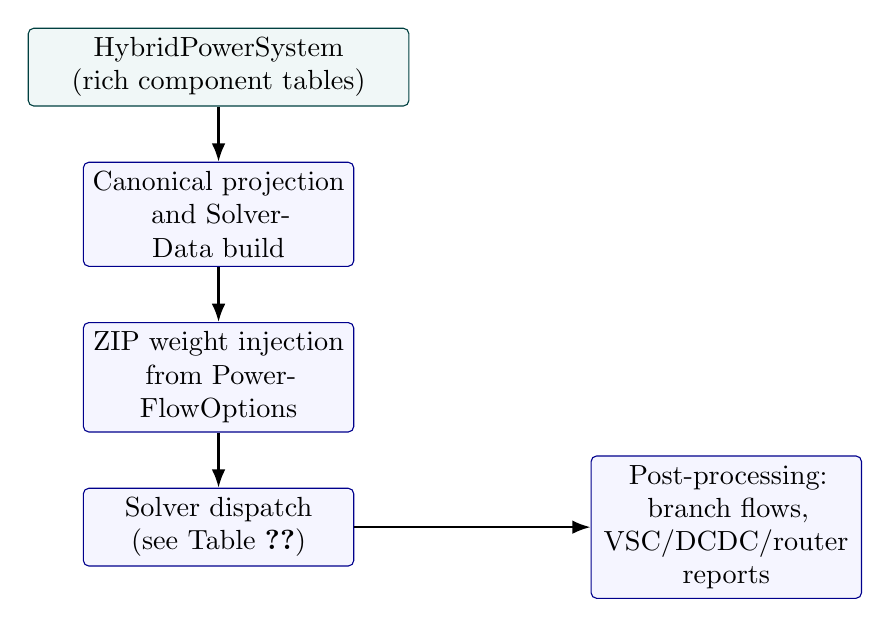
\begin{tikzpicture}[node distance=7mm and 12mm]
  \node[flowwide] (in) {\texttt{HybridPowerSystem}\\(rich component tables)};
  \node[flowbox, below=of in] (proj) {Canonical projection\\and \texttt{SolverData} build};
  \node[flowbox, below=of proj] (zip) {ZIP weight injection\\from \texttt{PowerFlowOptions}};
  \node[flowbox, below=of zip] (dispatch) {Solver dispatch\\(see Table~\ref{tab:pf-api})};
  \node[flowbox, right=30mm of dispatch] (post) {Post-processing:\\branch flows, VSC/DCDC/router reports};
  \draw[flowline] (in) -- (proj);
  \draw[flowline] (proj) -- (zip);
  \draw[flowline] (zip) -- (dispatch);
  \draw[flowline] (dispatch) -- (post);
\end{tikzpicture}
\caption{Shared execution pipeline for all power-flow API variants.}
\label{fig:pf-pipeline}
\end{figure}

% ------------------------------------------------------------
\subsection{Mathematical Problem Form}
% ------------------------------------------------------------

The Newton kernel solves the hybrid residual system
\begin{align}
F(x) = 0,
\qquad
x =
\begin{bmatrix}
\theta_{\mathcal{N}_{ac}\setminus\mathcal{N}_{sl}} \\
v_{\mathcal{N}_{PQ}} \\
v^{\qual{dc}}_{\mathcal{N}_{dc}\setminus\mathcal{N}_{sl}^{\qual{dc}}}
\end{bmatrix},
\label{eq:pf-residual}
\end{align}
where \(\mathcal{N}_{sl}\) and \(\mathcal{N}_{sl}^{\qual{dc}}\) are the sets of
AC and DC slack buses, and \(\mathcal{N}_{PQ}\) is the set of PQ buses.

\paragraph{AC bus mismatch.}
For each non-slack AC bus \(i\),
\begin{align}
\Delta P_i &= P_i^{\qual{spec}} - P_i^{\qual{calc}},
\qquad i\in\mathcal{N}_{ac}\setminus\mathcal{N}_{sl}, \\
\Delta Q_i &= Q_i^{\qual{spec}} - Q_i^{\qual{calc}},
\qquad i\in\mathcal{N}_{PQ},
\end{align}
where the calculated nodal injections are
\begin{align}
P_i^{\qual{calc}} &= \sum_{j\in\mathcal{N}_{ac}}
v_i v_j\!\left(G_{ij}\cos\theta_{ij}+B_{ij}\sin\theta_{ij}\right), \\
Q_i^{\qual{calc}} &= \sum_{j\in\mathcal{N}_{ac}}
v_i v_j\!\left(G_{ij}\sin\theta_{ij}-B_{ij}\cos\theta_{ij}\right),
\end{align}
with \(\theta_{ij}=\theta_i-\theta_j\) and \((G_{ij}+jB_{ij})\) the
\((i,j)\) entry of the sparse bus admittance matrix \(Y_{bus}\).

\paragraph{DC bus mismatch.}
For each non-DC-slack bus \(k\),
\begin{align}
\Delta P_k^{\qual{dc}} &= P_k^{\qual{dc,spec}} - P_k^{\qual{dc,calc}}, \\
P_k^{\qual{dc,calc}} &= v_k^{\qual{dc}}\!\left(G_{dc}\,v^{\qual{dc}}\right)_k.
\end{align}

\paragraph{Specified-injection assembly.}
\begin{align}
P_i^{\qual{spec}} &= P_i^{\qual{g,agg}} - P_i^{\qual{load}}(v_i) + P_i^{\qual{vsc}}, \\
Q_i^{\qual{spec}} &= Q_i^{\qual{g,agg}} - Q_i^{\qual{load}}(v_i) + Q_i^{\qual{vsc}},
\end{align}
where the aggregated generation vectors are
\begin{align}
P_i^{\qual{g,agg}} &= P_i^{\qual{gen}} + P_i^{\qual{sg}} + P_i^{\qual{ren}}
+ P_i^{\qual{pv}} + P_i^{\qual{stor}} + P_i^{\qual{vpp}}
+ P_i^{\qual{mg}} + P_i^{\qual{ms}}, \\
Q_i^{\qual{g,agg}} &= Q_i^{\qual{gen}} + Q_i^{\qual{sg}} + Q_i^{\qual{ren}}
+ Q_i^{\qual{pv}} + Q_i^{\qual{stor}} + Q_i^{\qual{vpp}}
+ Q_i^{\qual{ms}}.
\end{align}
Here \(P_i^{\qual{mg}}\) is microgrid exchange at the PCC bus in
\texttt{GridConnected} mode.

\paragraph{ZIP demand model.}
The runtime voltage-dependent load model is
\begin{align}
P_i^{\qual{load}}(v_i)
&= P_{i,0}\!\left(w_{P,0,i} + w_{P,1,i}v_i + w_{P,2,i}v_i^2\right), \\
Q_i^{\qual{load}}(v_i)
&= Q_{i,0}\!\left(w_{Q,0,i} + w_{Q,1,i}v_i + w_{Q,2,i}v_i^2\right).
\end{align}
The ZIP weights are populated in one of three assembly cases:
(1)~explicit \texttt{Load}/charging-station tables present,
(2)~charging-station tables only,
(3)~neither table — global \texttt{zip\_pw}/\texttt{zip\_qw} from
\texttt{PowerFlowOptions} are used.

% ------------------------------------------------------------
\subsection{VSC Converter Model}
% ------------------------------------------------------------

The converter model uses bus-injection-positive signs on both AC and DC sides.
Three control modes are supported.

\paragraph{Loss model.}
With active transfer \(p\) (p.u.), AC-side proxy current
\(I^{\qual{ac}}=|p|/v^{\qual{dc,safe}}\), \(v^{\qual{dc,safe}}=\max(v^{\qual{dc}},0.1)\):
\begin{align}
P^{\qual{loss,lin}} &= (1-\eta)|p|, \\
P^{\qual{loss,cur}} &= a + b\,I^{\qual{ac}} + c\,(I^{\qual{ac}})^2,
\qquad
a=\frac{\texttt{loss\_mw}}{S_{base}},\;
b=\frac{\texttt{loss\_pct}}{100},\;
c=1-\eta.
\end{align}

\paragraph{\texttt{PQ\_MODE}.}
\begin{align}
P^{\qual{conv,ac}} = P^{\qual{set}},\quad
Q^{\qual{conv,ac}} = Q^{\qual{set}},\quad
P^{\qual{conv,dc}} = -(P^{\qual{set}}+P^{\qual{loss}}).
\end{align}

\paragraph{\texttt{VDC\_Q} and \texttt{VDC\_VAC}.}
\begin{align}
P^{\qual{tr}} &= k^{\qual{vdc}}\!\left[(v^{\qual{dc}})^2-(v^{\qual{dc,set}})^2\right],\quad
P^{\qual{conv,ac}} = P^{\qual{tr}} - P^{\qual{loss}},\quad
P^{\qual{conv,dc}} = -P^{\qual{tr}}.
\end{align}
In \texttt{VDC\_VAC} mode the Newton loop enforces
\(v^{\qual{ac}}=v^{\qual{ac,set}}\) for the converter AC bus via an augmented
setpoint equation.

% ------------------------------------------------------------
\subsection{DCDC Converter Model}
% ------------------------------------------------------------

The DCDC converter connects \texttt{bus\_in} to \texttt{bus\_out}.
Power \texttt{p\_ref\_mw} is output-side referenced.
\begin{align}
P^{\qual{in}} &=
\begin{cases}
P^{\qual{ref}}/\eta, & P^{\qual{ref}}\ge 0, \\
P^{\qual{ref}}\cdot\eta, & P^{\qual{ref}}<0,
\end{cases}
\qquad
P^{\qual{out}} = P^{\qual{ref}} - r_{eq}\frac{(P^{\qual{in}})^2}{(v^{\qual{dc,in}})^2}.
\end{align}

% ------------------------------------------------------------
\subsection{Jacobian Structure}
% ------------------------------------------------------------

The linearized Newton system is
\begin{align}
J\,\Delta x = F(x),
\qquad
J =
\begin{bmatrix}
J_{\theta\theta} & J_{\theta V} & J_{\theta V^{dc}} \\
J_{V\theta} & J_{VV} & J_{V V^{dc}} \\
0 & J_{V^{dc} V} & J_{V^{dc} V^{dc}}
\end{bmatrix}.
\end{align}

The sparse Jacobian pattern is cached in a \texttt{PatternCache} keyed by
matrix storage addresses and a monotone \texttt{build\_id}, and is rebuilt only
on topology changes.

\paragraph{AC diagonal entries (with ZIP load corrections).}
\begin{align}
\frac{\partial \Delta P_i}{\partial v_i}
&= \frac{P_i^{\qual{calc}}}{v_i} + G_{ii}v_i
- P_{i,0}(w_{P,1,i}+2w_{P,2,i}v_i), \\
\frac{\partial \Delta Q_i}{\partial v_i}
&= \frac{Q_i^{\qual{calc}}}{v_i} - B_{ii}v_i
- Q_{i,0}(w_{Q,1,i}+2w_{Q,2,i}v_i).
\end{align}
In the code, \(v_i\) is floored at \texttt{min\_vm\_pu}
(configurable via \texttt{RobustNonlinearOptions}) to prevent zero-division.

\paragraph{DC entries.}
\begin{align}
\frac{\partial P_k^{\qual{dc,calc}}}{\partial v_m^{\qual{dc}}} =
\begin{cases}
(G_{dc}v^{\qual{dc}})_k + G_{kk}^{\qual{dc}}v_k^{\qual{dc}}, & m=k, \\
G_{km}^{\qual{dc}}v_k^{\qual{dc}}, & m\neq k.
\end{cases}
\end{align}

\paragraph{AC/DC coupling.}
When \texttt{enable\_coupled\_jacobian} is set, the converter Jacobian blocks
\(\partial P^{\qual{vsc}}/\partial v^{\qual{dc}}\),
\(\partial Q^{\qual{vsc}}/\partial v^{\qual{dc}}\), and
\(\partial P^{\qual{dc}}/\partial v^{\qual{ac}}\) are inserted analytically.
The coupling entries are pre-registered as \texttt{CouplingEntry} records in
\texttt{JacobianPattern} and updated in-place each iteration without
re-analyzing the pattern.

% ------------------------------------------------------------
\subsection{Hybrid Newton Algorithm}
\label{sec:pf-newton-algorithm}
% ------------------------------------------------------------

\begin{figure}[H]
\centering
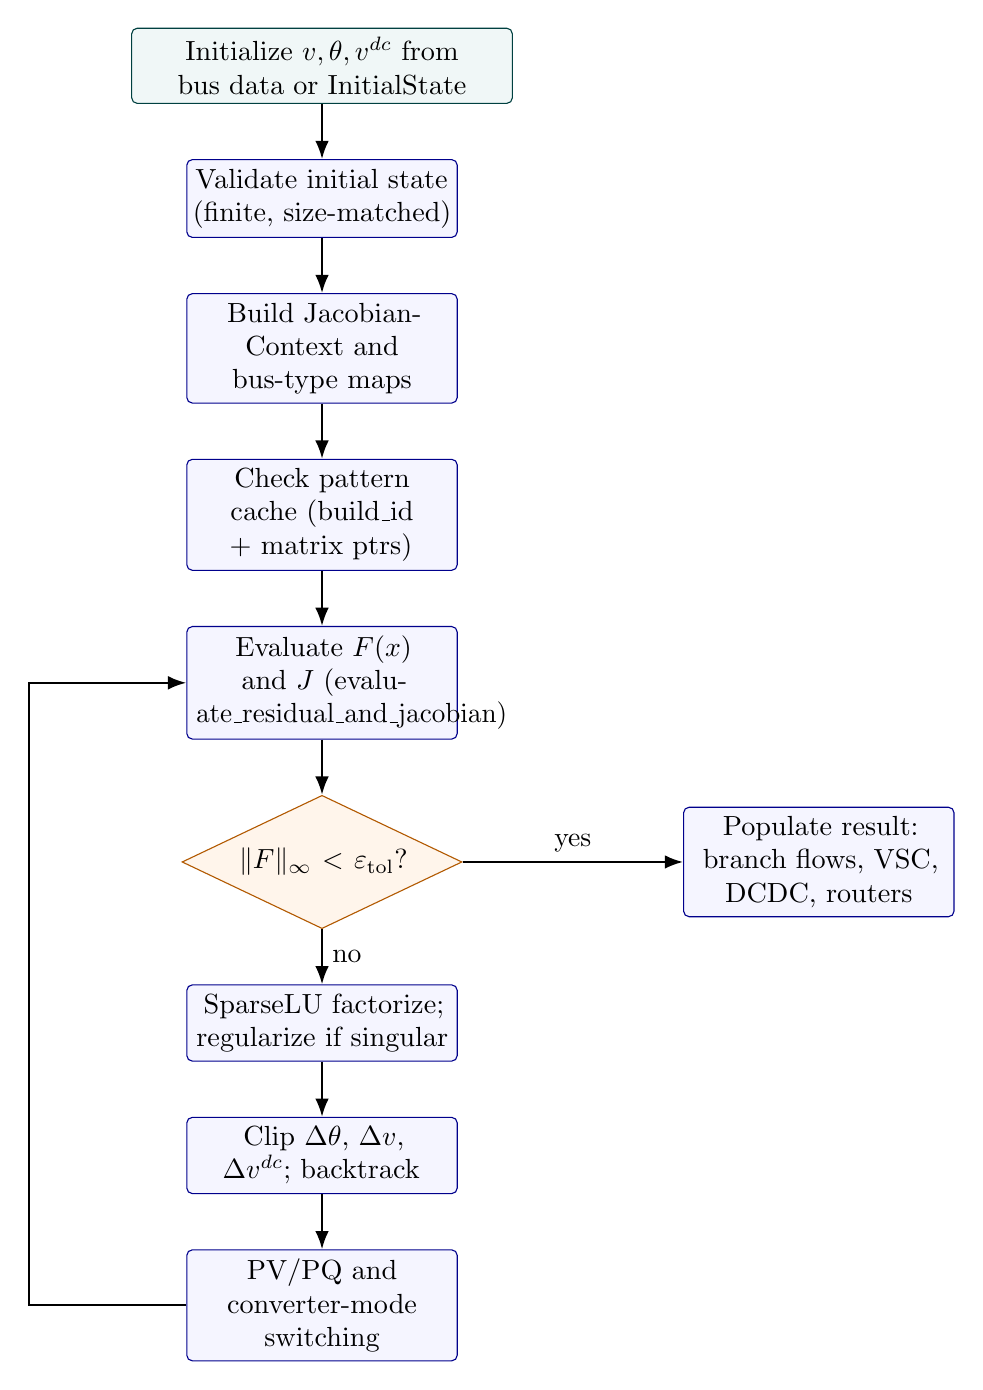
\begin{tikzpicture}[node distance=7mm and 13mm]
  \node[flowwide] (init)   {Initialize \(v,\theta,v^{dc}\) from bus data or \texttt{InitialState}};
  \node[flowbox, below=of init]  (validate) {Validate initial state (finite, size-matched)};
  \node[flowbox, below=of validate] (ctx)   {Build \texttt{JacobianContext} and bus-type maps};
  \node[flowbox, below=of ctx]   (cache)  {Check pattern cache (\texttt{build\_id} + matrix ptrs)};
  \node[flowbox, below=of cache]  (eval)  {Evaluate \(F(x)\) and \(J\) (\texttt{evaluate\_residual\_and\_jacobian})};
  \node[decision, below=of eval] (conv)  {\(\|F\|_\infty < \varepsilon_{\qual{tol}}\)?};
  \node[flowbox, right=28mm of conv] (done) {Populate result:\\ branch flows, VSC, DCDC, routers};
  \node[flowbox, below=of conv]  (factor){\texttt{SparseLU} factorize;\\ regularize if singular};
  \node[flowbox, below=of factor] (clip)  {Clip \(\Delta\theta\), \(\Delta v\), \(\Delta v^{dc}\); backtrack};
  \node[flowbox, below=of clip]  (switch){PV/PQ and converter-mode switching};
  \draw[flowline] (init)     -- (validate);
  \draw[flowline] (validate) -- (ctx);
  \draw[flowline] (ctx)      -- (cache);
  \draw[flowline] (cache)    -- (eval);
  \draw[flowline] (eval)     -- (conv);
  \draw[flowline] (conv)     -- node[above]{yes} (done);
  \draw[flowline] (conv)     -- node[right]{no}  (factor);
  \draw[flowline] (factor)   -- (clip);
  \draw[flowline] (clip)     -- (switch);
  \draw[flowline] (switch.west) |- ++(-20mm,0) |- (eval.west);
\end{tikzpicture}
\caption{Hybrid AC/DC Newton power-flow algorithm (\texttt{NewtonSolver::solve}).}
\label{fig:hybrid-newton}
\end{figure}

\paragraph{Algorithm PF-1: Hybrid Newton PF}
\begin{algorithmic}[1]
\Procedure{\texttt{NewtonSolver::solve}}{$\textit{data},\,\textit{opt},\,\textit{init}$}
  \State Validate \textit{init}: check size, NaN, Inf; \textbf{throw} \texttt{invalid\_argument} on failure
  \State $x \gets$ flat start or \textit{init} values; build \texttt{JacobianContext}
  \State $x_{\textit{ctx}}\texttt{.min\_vm\_pu} \gets \textit{opt.robust\_nonlinear.min\_vm\_pu}$
  \For{$k = 1,\ldots,\textit{opt.max\_iter}$}
    \State $F, J \gets \texttt{evaluate\_residual\_and\_jacobian}(x, \textit{ctx}, \textit{pattern})$
    \If{$\|F\|_\infty < \textit{opt.tol}$} \textbf{break} \EndIf
    \State $\texttt{SparseLU}(J)\,\Delta x = F$;\quad
      \textbf{if} singular \textbf{then} regularize and retry
    \State Clip $\Delta x$: $|\Delta\theta|\le\Delta\theta_{\max}$, $|\Delta v|\le\Delta v_{\max}$
    \State Backtracking line search; accept best step
    \State PV/PQ hysteresis switching; converter mode switching
  \EndFor
  \State \textbf{if} not converged \textbf{then} set \texttt{failure\_reason}
  \State Post-process branch, VSC, DCDC, router flows; \Return result
\EndProcedure
\end{algorithmic}

\paragraph{Robust nonlinear pipeline.}
The solver implements a five-phase robustification pipeline controlled by
\texttt{RobustNonlinearOptions}:
\begin{enumerate}
  \item \textbf{Phase 1 -- Scaling and diagnostics}: residual-equation scaling,
    variable scaling, and Jacobian row/column equilibration;
    condition-number proxy monitor.
  \item \textbf{Phase 2 -- Nonmonotone line search and smooth NCP}: Grippo--Lampariello--Lucidi
    nonmonotone Armijo search; optional \(\mu\)-perturbed Fischer--Burmeister
    complementarity for PV/PQ switching.
  \item \textbf{Phase 3 -- LM trust-region fallback}: Levenberg--Marquardt step
    \((J^\top J + \lambda I)\Delta x = -J^\top F\) when Newton line search fails;
    SER-based pseudo-transient continuation.
  \item \textbf{Phase 4 -- Homotopy continuation}: ramp loads and converter
    setpoints from flat start to target in adaptive \(\lambda\) steps.
  \item \textbf{Phase 5 -- Krylov fallback}: Newton--GMRES with Schur-complement
    AC/DC block preconditioner (opt-in; not active by default).
\end{enumerate}

% ------------------------------------------------------------
\subsection{Fast-Decoupled Power Flow (FDPF)}
% ------------------------------------------------------------

The FDPF solver builds two constant susceptance matrices from \(Y_{bus}\):
\begin{align}
B' &= -\Im\!\left\{Y_{bus}^{(R=0,\;b=0,\;\texttt{tap}=1)}\right\}, \\
B'' &= -\Im\!\left\{Y_{bus}^{(\text{full shunts and charging,\;zero phase shift})}\right\},
\end{align}
and then alternates P-\(\theta\) and Q-\(V\) decoupled solves:
\begin{align}
B'\,\Delta\theta &= \Delta P / v, \\
B''\,\Delta v &= \Delta Q / v.
\end{align}
Both \(B'\) and \(B''\) are factorized once via \texttt{Eigen::SparseLU}; only
the right-hand sides change across iterations.  The solver is AC-only (no DC or
converter coupling).

\paragraph{Algorithm PF-2: Fast-Decoupled PF}
\begin{algorithmic}[1]
\Procedure{\texttt{FDPFSolver::solve}}{$\textit{data},\,\textit{opt}$}
  \State Build reduced $B'_{\mathcal{N}\setminus\{sl\}}$, $B''_{\mathcal{N}_{PQ}}$; factorize
  \If{factorization failed} set \texttt{SingularJacobian}; \Return \EndIf
  \For{$k=1,\ldots,\textit{opt.fdpf\_max\_iter}$}
    \State Compute $\Delta P/v$, $\Delta Q/v$ using \textbf{sparse} $Y_{bus}$ iteration
    \If{$\|\Delta P/v\|_\infty < \varepsilon$ and $\|\Delta Q/v\|_\infty < \varepsilon$} \textbf{break} \EndIf
    \State $\Delta\theta \gets (B')^{-1}(\Delta P/v)$; update $\theta$
    \State $\Delta v \gets (B'')^{-1}(\Delta Q/v)$; update $v$
  \EndFor
\EndProcedure
\end{algorithmic}

% ------------------------------------------------------------
\subsection{DC-Only Power Flow}
% ------------------------------------------------------------

The DC solver iterates on non-slack DC voltages using dense LU on the small
reduced Jacobian:
\begin{align}
J_{dc}\,\Delta v^{\qual{dc}} &= \Delta P^{\qual{dc}}, \\
J_{dc,kl} &=
\begin{cases}
(G_{dc}v^{\qual{dc}})_k + G_{kk}^{\qual{dc}}v_k^{\qual{dc}}, & l=k, \\
G_{kl}^{\qual{dc}}v_k^{\qual{dc}}, & l\neq k.
\end{cases}
\end{align}
DC bus injections are assembled from \texttt{DCLoad}, DC storage, DC static
generators, DC PV arrays, VSC DC-side injections, DCDC transfers, and DC
\texttt{EnergyRouter} ports.
A backtracking line search over \(\alpha\in\{1,\tfrac12,\ldots\}\) is applied
with voltages floored at \texttt{kMinVdc} to prevent collapse.

% ------------------------------------------------------------
\subsection{Adaptive Islanded Solver}
% ------------------------------------------------------------

The adaptive solver handles multi-island AC/DC topologies that a single global
solve cannot address:

\begin{figure}[H]
\centering
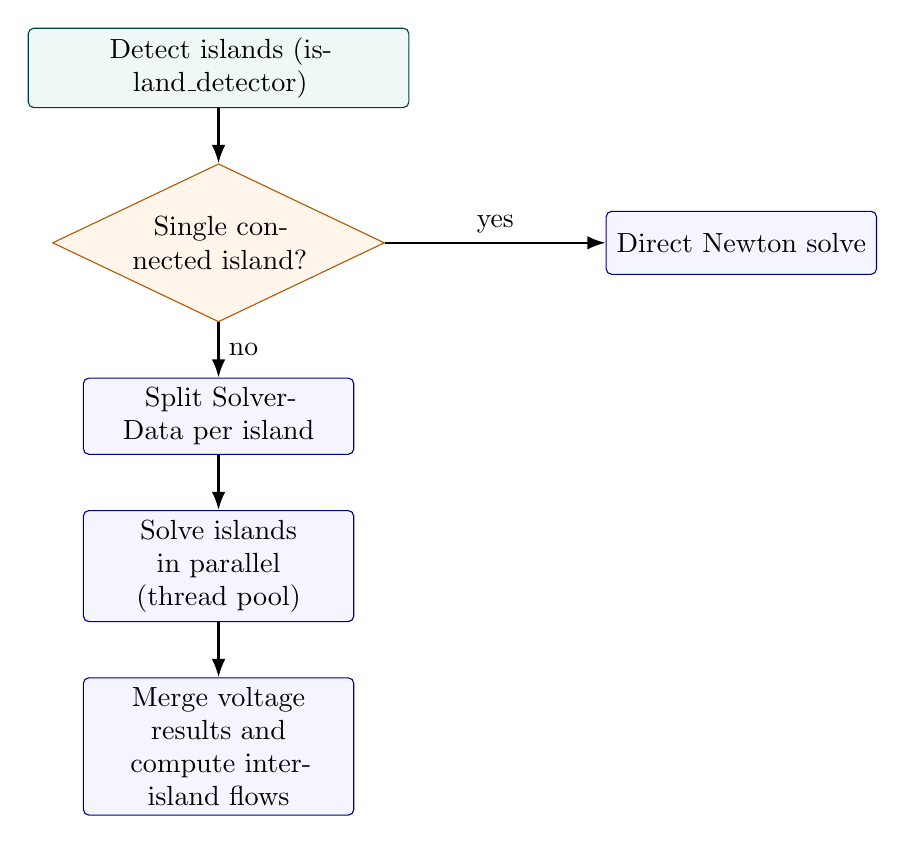
\begin{tikzpicture}[node distance=7mm and 13mm]
  \node[flowwide] (detect) {Detect islands (\texttt{island\_detector})};
  \node[decision, below=of detect] (single) {Single connected island?};
  \node[flowbox, right=28mm of single] (direct) {Direct Newton solve};
  \node[flowbox, below=of single] (split) {Split \texttt{SolverData} per island};
  \node[flowbox, below=of split] (par) {Solve islands in parallel\\(thread pool)};
  \node[flowbox, below=of par] (merge) {Merge voltage results and\\compute inter-island flows};
  \draw[flowline] (detect) -- (single);
  \draw[flowline] (single) -- node[above]{yes} (direct);
  \draw[flowline] (single) -- node[right]{no} (split);
  \draw[flowline] (split) -- (par);
  \draw[flowline] (par) -- (merge);
\end{tikzpicture}
\caption{Adaptive islanded power-flow workflow.}
\label{fig:adaptive-pf}
\end{figure}

% ------------------------------------------------------------
\subsection{HELM Solver}
% ------------------------------------------------------------

The HELM (Holomorphic Embedding Load-flow Method) solver constructs a power
series in a complex embedding parameter \(s\in\mathbb{C}\):
\begin{align}
V_i(s) = \sum_{n=0}^{N} a_n^{(i)}\,s^n.
\end{align}
The recursion for order \(n\) coefficients follows from the holomorphic
embedding of the network equations.  Convergence is tested via Padé approximants
\([M/M]\) evaluated at \(s=1\):
\begin{align}
V_i(1) \approx \frac{P_M(1)}{Q_M(1)}.
\end{align}
The HELM solver is used as a DC warm-start supplier for the hybrid Newton path
(\texttt{HelmWarmStart::DCPF}) and as a standalone fallback in the adaptive
solver chain.

% ------------------------------------------------------------
\subsection{Error Handling and Diagnostics}
% ------------------------------------------------------------

All solvers return a result struct with a \texttt{SolverFailureReason} field
(added in the May~2026 hardening pass):
\begin{itemize}
  \item \texttt{None} --- converged successfully,
  \item \texttt{SingularJacobian} --- \texttt{SparseLU} or dense LU
    factorization reported failure (B\({}'\), B\({}''\), or DC Jacobian),
  \item \texttt{NonFiniteSolution} --- Newton step or intermediate state
    contained NaN or Inf,
  \item \texttt{InvalidInitialState} --- provided \texttt{InitialState} contained
    non-finite values (guarded by \texttt{validate\_initial\_state}),
  \item \texttt{MaxIterationsReached} --- tolerance not met within the iteration limit.
\end{itemize}

The solver \textbf{throws} \texttt{std::invalid\_argument} for structural API
violations (e.g., size mismatch, NaN in initial state) and \textbf{returns
a non-converged result} for numerical failures.  This two-tier policy separates
programming errors from expected numerical difficulties.

% ------------------------------------------------------------
\subsection{Maintainability Roadmap: Code-Duplication Inventory}
\label{sec:pf-dedup}
% ------------------------------------------------------------

All six items D1--D6 from the original inventory were resolved across two
refactoring passes (\textit{code-dedup-D1-D5} and \textit{code-dedup-D3-D6}).

\paragraph{D1 --- \texttt{inf\_norm} \textnormal{(}\textbf{DONE}\textnormal{)}.}
The anonymous-namespace duplicate removed from
\texttt{jacobian\_builder.cpp} and \texttt{dc\_solver.cpp}.
The canonical definition now lives in
\texttt{include/hacdcpf/power_flow/pf\_utils.hpp} as an inline function.
Test files \texttt{test\_powerflow\_performance.cpp} updated to use
\texttt{hacdcpf::powerflow::inf\_norm} via a \texttt{using} declaration.

\paragraph{D2 --- DC injection assembly \textnormal{(}\textbf{DONE}\textnormal{)}.}
The 80-line DC injection loop extracted into
\texttt{assemble\_dc\_injections(data, vm, va, vdc, pdc\_spec)},
declared in a new header
\texttt{include/hacdcpf/power_flow/pf\_injection\_assembly.hpp} and
implemented in \texttt{src/power_flow/pf\_injection\_assembly.cpp}.
Both \texttt{dc\_solver.cpp} and \texttt{residual\_evaluator.cpp} now
call this single canonical function.

\paragraph{D3 --- Duplicated B\('\) matrix construction \textnormal{(}\textbf{DONE}\textnormal{)}.}
The anonymous-namespace functions \texttt{build\_bp} and \texttt{build\_bpp}
were removed from \texttt{fdpf\_solver.cpp} and replaced with calls to a
new utility \texttt{build\_susceptance\_matrix(data, flags)} implemented in
\texttt{admittance\_builder.cpp}.  A \texttt{BpBuildFlags} struct (declared in
\texttt{admittance\_builder.hpp}) controls all assembly variants: zero
resistance, zero line charging, unit tap, zero phase shift, and optional bus
shunt susceptance.  Convenience factories \texttt{make\_bp\_flags(min\_x\_pu)}
and \texttt{make\_bpp\_flags()} cover the two FDPF use cases.

\paragraph{D4 --- DC initial-state warm-start \textnormal{(}\textbf{DONE}\textnormal{)}.}
The size-guarded copy of \texttt{init->vdc} with NaN/Inf validation
extracted into \texttt{load\_dc\_initial\_state(init, dc\_buses, vdc)}
in \texttt{pf\_utils.hpp}.  Applied to both \texttt{dc\_solver.cpp} and
\texttt{newton\_solver.cpp}.

\paragraph{D5 --- Bus-type classification loop \textnormal{(}\textbf{DONE}\textnormal{)}.}
The manual AC bus classification into SLACK/PV/PQ sets extracted into
\texttt{classify\_ac\_buses(data)} returning an \texttt{AcBusSets} struct
(all in \texttt{pf\_utils.hpp}).  Applied to \texttt{fdpf\_solver.cpp},
\texttt{residual\_evaluator.cpp}, and the helper in
\texttt{test\_unified\_pf\_upgrade.cpp}.

\paragraph{D6 --- \texttt{jacobian\_builder.cpp} file split \textnormal{(}\textbf{DONE}\textnormal{)}.}
The monolithic \texttt{jacobian\_builder.cpp} was split into three focused
compilation units:
\begin{itemize}
  \item \texttt{jacobian\_pattern.cpp} --- \texttt{build\_jacobian\_pattern} and
        its anonymous-namespace helpers (\texttt{rc\_key},
        \texttt{add\_pattern\_position}, \texttt{build\_entry\_to\_nz},
        \texttt{lookup\_nz});
  \item \texttt{ac\_kernel.cpp} --- \texttt{evaluate\_ac\_kernel\_serial},
        \texttt{evaluate\_ac\_kernel\_parallel}, and \texttt{effective\_ac\_threads};
  \item \texttt{jacobian\_builder.cpp} (retained) --- \texttt{build\_power\_spec},
        \texttt{evaluate\_residual\_impl}, \texttt{evaluate\_residual\_and\_jacobian},
        and \texttt{evaluate\_residual\_only}.
\end{itemize}
The cross-file linkage between \texttt{jacobian\_builder.cpp} and
\texttt{ac\_kernel.cpp} is provided by an internal header
\texttt{src/power_flow/ac\_kernel\_impl.hpp} (not installed).

% ------------------------------------------------------------
\subsection{Numerical Performance (Release Mode)}
\label{sec:pf-performance}
% ------------------------------------------------------------

Benchmarks were run on 84 MATPOWER cases (\texttt{build\_rel},
Apple M4, \texttt{-O3 -DNDEBUG}, single thread) using
\texttt{build\_rel/helm\_powerflow\_benchmark ../data}.
Four paths are compared: NR = hybrid Newton, FD = fast-decoupled,
HE = HELM standalone, HE+DC = HELM with DC warm start.

\begin{longtable}{L{0.18\linewidth}rr
  L{0.08\linewidth}L{0.08\linewidth}
  L{0.08\linewidth}L{0.08\linewidth}}
\toprule
Case & $N$ & Branches & NR ms & FD ms & HE ms & HE+DC ms \\
\midrule
\endhead
case14 & 14 & 20 & 0.0 & 0.3 & 0.1 & 0.1 \\
case57 & 57 & 80 & 0.1 & 2.9 & 0.6 & 0.6 \\
case118 & 118 & 186 & 0.4 & 11.5 & 1.8 & 1.9 \\
case300 & 300 & 411 & 0.9 & 59.5 & div & div \\
case1354pegase & 1354 & 1991 & 15.2 & skip & div & div \\
case1888rte & 1888 & 2531 & 10.8 & skip & 135.8 & 136.5 \\
case2383wp & 2383 & 2896 & 3.8 & skip & 117.6 & 109.3 \\
case2736sp & 2736 & 3504 & 5.6 & skip & 75.2 & 76.6 \\
case3012wp & 3012 & 3572 & 35.0 & skip & 124.3 & 126.9 \\
case6468rte & 6468 & 9000 & 31.7 & skip & 297.7 & 296.2 \\
case8387pegase & 8387 & 14561 & 46.7 & skip & 1776.5 & 1786.7 \\
case13659pegase & 13659 & 20467 & 95.9 & skip & skip & skip \\
case\_ACTIVSg10k & 10000 & 12706 & 21.8 & skip & 4327.9 & 4389.7 \\
case\_ACTIVSg25k & 25000 & 32230 & 64.3 & skip & skip & skip \\
case\_SyntheticUSA & 82000 & 104121 & 1745.2 & skip & skip & skip \\
\bottomrule
\caption{Power-flow solver timing (release mode, Apple M4, single thread, post D1--D5 refactor).
``div'' = diverged, ``skip'' = case excluded from path at this size.}
\label{tab:pf-perf}
\end{longtable}

Key observations:
\begin{itemize}
  \item The hybrid Newton path converges on the 82000-bus USA synthetic system
    in 1.75\,s with 17 iterations after the D1--D5 refactoring pass
    (no regression vs.\ pre-refactoring baseline).
  \item Newton solve time scales approximately as $O(N^{1.2})$ in practice for
    typical sparse transmission systems.
  \item FDPF is 10--200$\times$ slower than Newton on small-to-medium cases due
    to the current $O(N^2)$ dense Ybus iteration in the power-injection loop;
    replacing it with a sparse row iteration remains an open performance item.
  \item HELM converges on most well-conditioned cases under 2000~buses but
    diverges on stressed systems (case300, case1354pegase); it
    remains useful as a warm-start provider for Newton on difficult cases.
  \item The D1--D6 refactoring passes introduced no performance regression:
    Newton solve times match the pre-refactoring baseline on all benchmark cases.
\end{itemize}

\section{Optimal Power Flow Models}
\label{sec:opf}

\subsection{Problem Form and Runtime Scope}

This chapter covers the OPF family built on top of canonical AC/DC network
projection.  The implemented runtime problem classes are:
\begin{itemize}
  \item nonlinear AC/DC OPF for the native primal-dual and parity-IPM routes,
  \item DC OPF with a true-QP model and LP fallback backends,
  \item reactive-power optimization over discrete taps and shunts by
  outer-approximation / coordinate-search heuristics.
\end{itemize}
The runtime solver family is selected from option flags and DC-network presence.

\subsection{Code Map}

The current implementation is concentrated in:
\begin{itemize}
  \item \texttt{src/optimal_power_flow/ac\_opf.cpp} for top-level AC OPF routing and native reduced-space solve orchestration,
  \item \texttt{src/optimal_power_flow/parity\_formulation.cpp} and \texttt{src/optimal_power_flow/parity\_ipm.cpp} for the parity full-space NLP route,
  \item \texttt{src/optimal_power_flow/dc\_opf.cpp} for DC OPF model build and backend selection,
  \item \texttt{src/optimal_power_flow/reactive\_power\_opt.cpp} for the four-phase outer-approximation / coordinate-search workflow,
  \item \texttt{include/hacdcpf/engine} forwarding headers for LCQP, dual simplex, HiGHS, Gurobi, and related engine facilities supplied by the \texttt{mipsolvers} dependency.
\end{itemize}
There is no \texttt{src/engine} directory in this repository.

\subsection{Pseudocode Map}

The relevant code-aligned workflows are:
\begin{itemize}
  \item Algorithms A8--A10 in Section~\ref{sec:algorithms} for AC OPF routing, parity-NLP construction, and parity-IPM solve,
  \item Algorithm A11 for DC OPF,
  \item Algorithm A12 for reactive-power optimization,
  \item Section~\ref{sec:engine-solver-system} for the forwarding engine surface used by DC OPF and RPO result statistics.
\end{itemize}

\subsection{Current Status}

The AC OPF family has multiple implemented routes, but backend coverage differs
by path.  Parity and native nonlinear routes are the main AC/DC engines; DC OPF
builds a specialized QP/LP model; RPO currently runs an OA/coordinate-search
workflow and reuses branch-and-cut-style statistics fields for counters.

\subsection{Top-Level Solver Routing}

The public \texttt{solve\_ac\_opf} path selects among three solver families.
A key implementation rule is automatic DC routing: if the case has DC buses or
VSC converters and \texttt{enable\_primal\_dual=false}, the options are
internally overridden to
\texttt{enable\_primal\_dual=true, use\_parity\_ipm=true}.

\begin{longtable}{L{0.25\linewidth}L{0.26\linewidth}L{0.37\linewidth}}
\toprule
Path & Trigger & Current behavior \\
\midrule
\endhead
Fast dispatch + PF fallback (AC-only) &
\texttt{enable\_primal\_dual=false} and no forced DC parity routing &
Drops DC and converter subsystems, solves economic dispatch, then runs AC PF projection. \\
Native primal-dual OPF &
\texttt{enable\_primal\_dual=true}, \texttt{use\_parity\_ipm=false} &
Uses a custom sparse KKT loop with AC equations, DC-bus equations, and converter power-balance equations. \\
Parity primal-dual IPM &
\texttt{enable\_primal\_dual=true}, \texttt{use\_parity\_ipm=true}
or auto-enabled by DC presence &
Builds the parity full-space NLP and solves by Mehrotra-type primal-dual IPM. Optional fallback to native path when enabled. \\
\bottomrule
\end{longtable}

\subsection{Fast Dispatch + PF Fallback (AC-Only Path)}

This path is used for fastest feasible dispatch recovery in AC-only operation.
It solves a clipped economic dispatch first, then projects via AC PF.

\paragraph{Economic dispatch stage.}
\begin{align}
\min_{P_g}\; \sum_{g\in\mathcal{G}}
\left(c_{2g}P_g^2 + c_{1g}P_g + c_{0g}\right),
\end{align}
subject to generator bounds and
\(\sum_g P_g = P_D\) (clamped to feasible range).
For quadratic units, the code uses incremental-cost clipping
\(P_g = \mathrm{clip}((\lambda-c_1)/(2c_2),P_g^{\qual{min}},P_g^{\qual{max}})\).

\paragraph{Feasibility projection stage.}
The dispatch is passed to AC Newton PF; resulting bus injections are split back
across generators at each bus and clamped to individual bounds.
If direct projection fails, one reshaped economic-dispatch attempt is executed
before declaring failure.

\subsection{Native Primal-Dual OPF Formulation}

\subsubsection{Decision Variables}

For the native path, variables are
\begin{align}
x_{nat}=
\begin{bmatrix}
\theta_{\mathcal{N}_{ac}\setminus\mathcal{N}_{sl}} &
v_{\mathcal{N}_{PQ}} &
P_g & Q_g &
v^{\qual{dc}} &
P^{\qual{conv,ac}} & Q^{\qual{conv,ac}} & P^{\qual{conv,dc}}
\end{bmatrix}^{\top}.
\end{align}

The implementation includes all DC bus voltages in \(v^{\qual{dc}}\); for
\texttt{DC\_V} buses, tight bounds are built around the setpoint.

\subsubsection{Objective}
\begin{align}
\min_x f(x) =
\sum_{g\in\mathcal{G}}
\left(c_{2g}P_g^2 + c_{1g}P_g + c_{0g}\right).
\end{align}

\subsubsection{Equality Constraints}

\paragraph{AC equations.}
AC rows reuse the PF residual kernel (with converter table disabled in that
kernel call), then subtract explicit converter variables:
\begin{align}
g_{P,i} &= \left(P_i^{\qual{spec,PF}}-P_i^{\qual{calc}}\right) - \sum_{c\in\mathcal{C}_i} P_c^{\qual{ac}} = 0,
&& i\in\mathcal{N}_{ac}\setminus\mathcal{N}_{sl}, \\
g_{Q,i} &= \left(Q_i^{\qual{spec,PF}}-Q_i^{\qual{calc}}\right) - \sum_{c\in\mathcal{C}_i} Q_c^{\qual{ac}} = 0,
&& i\in\mathcal{N}_{PQ}.
\end{align}

\paragraph{DC equations.}
For each DC bus \(k\):
\begin{align}
g_{k}^{\qual{dc}} = P_{d,k}^{\qual{dc}} + V_k^{\qual{dc}}(G_{dc}V^{\qual{dc}})_k
- \sum_{c\in\mathcal{C}_k^{\qual{dc}}} P_c^{\qual{dc}} = 0.
\end{align}

\paragraph{Converter energy balance.}
For converter \(c\):
\begin{align}
g_c^{\qual{conv}} &= P_c^{\qual{ac}} + P_c^{\qual{dc}} + P_c^{\qual{loss}} = 0, \\
P_c^{\qual{loss}} &= a_c + b_c I_c^{\qual{ac}} + (1-\eta_c)(I_c^{\qual{ac}})^2, \\
I_c^{\qual{ac}} &= \frac{\sqrt{(P_c^{\qual{ac}})^2+(Q_c^{\qual{ac}})^2+\epsilon}}{V_c^{\qual{ac}}},
\quad \epsilon=10^{-6}.
\end{align}

\subsubsection{Bounds and Nonlinear Limits}

Variable bounds are enforced for
\(\theta, v, P_g, Q_g, v^{\qual{dc}}, P^{\qual{conv,ac}}, Q^{\qual{conv,ac}}, P^{\qual{conv,dc}}\).

Nonlinear engineering limits are modeled as
\(h(x)\le 0\) and handled by exterior quadratic penalty terms inside the
merit model:
\begin{align}
h_{ij}^{\qual{from}} &= P_{f,ij}^2 + Q_{f,ij}^2 - (S_{ij}^{\qual{max}})^2 \le 0, \\
h_{ij}^{\qual{to}}   &= P_{t,ij}^2 + Q_{t,ij}^2 - (S_{ij}^{\qual{max}})^2 \le 0, \\
h_c^{\qual{conv}}    &= (P_c^{\qual{ac}})^2 + (Q_c^{\qual{ac}})^2 - (S_c^{\qual{max}})^2 \le 0.
\end{align}

\subsubsection{KKT System and Globalization}

At each inner iteration, the solver builds
\begin{align}
\begin{bmatrix}
H + \delta I & J_g^{\top} \\
J_g & -\delta I
\end{bmatrix}
\begin{bmatrix}
\Delta x \\
\Delta\lambda
\end{bmatrix}
=
-\begin{bmatrix}
\nabla_x L \\
g(x)
\end{bmatrix},
\end{align}
with dynamic regularization \(\delta\), line search, trust/restore logic,
and bounded step clipping.

A barrier term is applied to variable bounds; nonlinear branch/converter limits
enter the merit model through adaptive exterior penalties.

\subsection{Parity Full-Space Formulation}

\subsubsection{Decision Variables}

The parity NLP includes AC, DC, converter, shedding, and enhanced DER variables:
\begin{align}
x_{par}=
\begin{bmatrix}
\theta,\ v^{\qual{ac}},\ P_g,\ Q_g,\ v^{\qual{dc}},\ P^{\qual{conv,ac}},\ Q^{\qual{conv,ac}},\ P^{\qual{conv,dc}}, \\
\Delta P_d,\ \Delta Q_d,\ P^{\qual{ren}},\ Q^{\qual{ren}},\ P^{\qual{stor,ac}},\ Q^{\qual{stor,ac}},\ P^{\qual{stor,dc}}, \\
P^{\qual{dcdc}},\ P^{\qual{flex}}
\end{bmatrix}^{\top}.
\end{align}

\subsubsection{Objective}
\begin{align}
\min_x f_{par}(x) =
&\sum_{g\in\mathcal{G}}\left(c_{2g}P_g^2 + c_{1g}P_g + c_{0g}\right)
+ \mathrm{VOLL}_{eff} S_{base}\sum_i (\Delta P_{d,i}+\Delta Q_{d,i}) \\
&+ \sum_{r\in\mathcal{R}^{\qual{curt}}}
\max\left(0, P_{r}^{\qual{rated}} - P_r\right)c_r^{\qual{curt}}.
\end{align}

\subsubsection{Equality Constraints}

\paragraph{AC full-bus balance (scaled).}
For each AC bus \(i\):
\begin{align}
g_{P,i} &=
\Bigl(P_i^{\qual{calc}} - P_i^{\qual{gen}} - P_i^{\qual{fixed}} - P_i^{\qual{ren}} - P_i^{\qual{stor}}
+ P_i^{\qual{load}} - \Delta P_{d,i} + P_i^{\qual{flex}} - P_i^{\qual{conv,ac}}\Bigr)\,\alpha_P = 0, \\
g_{Q,i} &=
\Bigl(Q_i^{\qual{calc}} - Q_i^{\qual{gen}} - Q_i^{\qual{fixed}} - Q_i^{\qual{ren}} - Q_i^{\qual{stor}}
+ Q_i^{\qual{load}} - \Delta Q_{d,i} - Q_i^{\qual{conv,ac}}\Bigr)\,\alpha_Q = 0.
\end{align}
Here \(P_i^{\qual{fixed}},Q_i^{\qual{fixed}}\) aggregate non-variable injections
(static generators, non-curtailable renewables/PV, VPP, microgrid exchange,
mobile storage).

\paragraph{DC balance with DCDC coupling.}
For each DC bus \(k\):
\begin{align}
g_k^{\qual{dc}} = P_{d,k}^{\qual{dc}} + \sum_{m\neq k} g_{km}
\left((V_k^{\qual{dc}})^2 - V_k^{\qual{dc}}V_m^{\qual{dc}}\right)
- P_k^{\qual{conv,dc}} + P_k^{\qual{dcdc,in}} - P_k^{\qual{dcdc,out}} = 0,
\end{align}
where the OPF decision variable is \(P^{\qual{in}}\)
(\emph{input-side referenced}, i.e.\ the power absorbed from \texttt{bus\_in}).
The output power is a deterministic function of \(P^{\qual{in}}\) including
both efficiency and \(I^2R\) conduction loss:
\begin{align}
P^{\qual{out}}=
\begin{cases}
\eta\, P^{\qual{in}} - r_{eq}(P^{\qual{in}})^2/(V^{\qual{dc}})^2,
& P^{\qual{in}}\ge 0, \\
P^{\qual{in}}/\eta - r_{eq}(P^{\qual{in}})^2/(V^{\qual{dc}})^2,
& P^{\qual{in}}<0.
\end{cases}
\end{align}
The parity \texttt{ConstraintIndex} allocates dedicated DCDC balance slots and
counts them in the equality total, but the current equality evaluator leaves
those dedicated rows unpopulated.  The actual DCDC physics is folded directly
into the two DC bus balance equations:
\begin{align}
g_{\texttt{bus\_in}} &\mathrel{+}= P^{\qual{in}}, &
g_{\texttt{bus\_out}} &\mathrel{-}= P^{\qual{out}}.
\end{align}

\paragraph{DCDC Jacobian and Hessian.}
The first-order derivatives of the DCDC coupling terms are:
\begin{align}
\frac{\partial g_{\texttt{bus\_in}}}{\partial P^{\qual{in}}} &= 1, &
\frac{\partial g_{\texttt{bus\_out}}}{\partial P^{\qual{in}}} &=
-\frac{\partial P^{\qual{out}}}{\partial P^{\qual{in}}}, \\
\frac{\partial P^{\qual{out}}}{\partial P^{\qual{in}}} &=
\begin{cases}
\eta - 2r_{eq}P^{\qual{in}}/(V^{\qual{dc}})^2, & P^{\qual{in}}\ge 0, \\
1/\eta - 2r_{eq}P^{\qual{in}}/(V^{\qual{dc}})^2, & P^{\qual{in}}<0.
\end{cases}
\end{align}
When \(r_{eq}>0\), there is also a cross-derivative with respect to
the input-side DC voltage:
\begin{align}
\frac{\partial g_{\texttt{bus\_out}}}{\partial V^{\qual{dc}}_{\texttt{in}}}
&= \frac{2r_{eq}(P^{\qual{in}})^2}{(V^{\qual{dc}}_{\texttt{in}})^3}.
\end{align}
The Hessian contributions from the \(I^2R\) loss term are:
\begin{align}
\frac{\partial^2 g}{\partial (P^{\qual{in}})^2}
&= \frac{2r_{eq}}{(V^{\qual{dc}})^2}, &
\frac{\partial^2 g}{\partial P^{\qual{in}}\partial V^{\qual{dc}}}
&= \frac{-4r_{eq}P^{\qual{in}}}{(V^{\qual{dc}})^3}, &
\frac{\partial^2 g}{\partial (V^{\qual{dc}})^2}
&= \frac{6r_{eq}(P^{\qual{in}})^2}{(V^{\qual{dc}})^4}.
\end{align}

\paragraph{OPF warm-start convention.}
Note that the PF uses output-referenced \(P^{\qual{ref}}\) while the OPF uses
input-referenced \(P^{\qual{in}}\).  The warm-start path converts between these
reference frames when seeding the OPF initial point from a PF result.

\paragraph{Converter balance.}
For each VSC converter:
\begin{align}
P_c^{\qual{ac}}+P_c^{\qual{dc}}+P_c^{\qual{loss}}=0,
\end{align}
with the same loss model as in the native formulation.

\subsubsection{Inequality Constraints}

Nonlinear inequalities:
\begin{align}
P_{f,ij}^2 + Q_{f,ij}^2 - (S_{ij}^{\qual{max}})^2 &\le 0, \\
P_{t,ij}^2 + Q_{t,ij}^2 - (S_{ij}^{\qual{max}})^2 &\le 0, \\
(P_c^{\qual{ac}})^2 + (Q_c^{\qual{ac}})^2 - (S_c^{\qual{max}})^2 &\le 0, \\
\left(g_{km}V_k^{\qual{dc}}(V_k^{\qual{dc}}-V_m^{\qual{dc}})\right)^2 - (P_{km}^{\qual{max}})^2 &\le 0.
\end{align}

Variable bounds are converted to inequality rows:
\begin{align}
x^{\qual{min}}-x \le 0, \qquad x-x^{\qual{max}}\le 0.
\end{align}

\subsubsection{Primal-Dual IPM System}

The parity solver introduces slack \(z>0\) and multipliers \(\mu>0\):
\begin{align}
g(x) &= 0, \\
h(x)+z &= 0, \\
\nabla f(x)+J_g^{\top}\lambda+J_h^{\top}\mu &= 0, \\
z \circ \mu &= \gamma\mathbf{1}.
\end{align}

A Mehrotra predictor-corrector method is used, with:
\begin{enumerate}
  \item affine predictor step,
  \item adaptive centering parameter
  \(\sigma = (\mu_{aff}/(\mu_{cur}+10^{-16}))^3\) after clamping the ratio to \([0,1]\),
  \item corrector step with second-order compensation,
  \item iterative refinement (2 steps) for conditioning of the KKT solve,
  \item fraction-to-boundary step lengths for primal and dual updates.
\end{enumerate}

\paragraph{Implementation note.}
The current \texttt{parity\_ipm.cpp} uses the Mehrotra predictor-corrector
scheme and implements up to two Gondzio extra correctors.
The KKT system is solved using either Eigen \texttt{SparseLU} for sparse or
\texttt{PartialPivLU} for dense factorizations.

Convergence monitors primal infeasibility, dual stationarity, and average
complementarity. A best-iterate restoration is applied before final failure.

\subsection{Component Coverage by Solver Path}

\begin{longtable}{L{0.30\linewidth}L{0.22\linewidth}L{0.36\linewidth}}
\toprule
Component / feature & Native primal-dual & Parity IPM \\
\midrule
\endhead
\texttt{Generator} \((P_g,Q_g)\) & decision variable & decision variable \\
\texttt{VSCConverter} \((P^{\qual{conv,ac}},Q^{\qual{conv,ac}},P^{\qual{conv,dc}})\) & decision variable & decision variable \\
\texttt{DCBus} voltage & decision variable & decision variable \\
AC branch MVA limits & nonlinear penalty term & nonlinear inequality + slack \\
DC branch power limits & not explicit in native path & nonlinear inequality + slack \\
Load shedding \((\Delta P_d,\Delta Q_d)\) & not modeled & decision variable with VOLL penalty \\
Curtailable renewable / controllable PV & not modeled as variable & decision variable \\
AC storage dispatch & not modeled as variable & decision variable \\
DC storage dispatch & not modeled as variable & decision variable; packed into \texttt{ACOPFResult::pstor\_mw} with \texttt{stor\_map.source\_type} identifying AC vs DC storage \\
DCDC dispatch & not modeled as variable & decision variable + DC coupling \\
Flexible load dispatch & not modeled as variable & decision variable \\
StaticGen / fixed DER aggregates & not explicit variable in native objective model & included as fixed injections \\
\bottomrule
\end{longtable}

\subsection{AC OPF Result JSON Contract}

\texttt{opf\_result\_to\_json} writes the scalar solve summary
\texttt{converged}, \texttt{iterations}, \texttt{outer\_iterations},
\texttt{objective}, \texttt{max\_constraint\_violation},
\texttt{max\_stationarity}, \texttt{status}, and \texttt{solver\_path}.  The
\texttt{solver\_path} token is \texttt{NativeAC}, \texttt{ParityIPM}, or
\texttt{Unknown}.

The core vectors are \texttt{vm}, \texttt{va}, \texttt{vdc}, \texttt{pg\_mw},
\texttt{qg\_mvar}, \texttt{dpd\_mw}, \texttt{dqd\_mvar}, \texttt{pac\_mw}, and
\texttt{qac\_mvar}.  Enhanced dispatch is serialized both as structured objects
and as legacy bare arrays:
\begin{itemize}
  \item \texttt{renewable\_dispatch}: \texttt{pren\_mw}, \texttt{qren\_mvar}, and
  a \texttt{map} array of \texttt{original\_index}/\texttt{source\_type} records;
  \item \texttt{storage\_dispatch}: \texttt{pstor\_mw}, \texttt{qstor\_mvar}, and
  a \texttt{map} array; this packed storage array includes AC and DC storage;
  \item \texttt{dcdc\_dispatch}: \texttt{pdcdc\_mw} and a \texttt{map} array;
  \item \texttt{flex\_dispatch}: \texttt{pflex\_mw} and a \texttt{map} array;
  \item legacy top-level \texttt{pren\_mw}, \texttt{qren\_mvar}, \texttt{pstor\_mw},
  \texttt{qstor\_mvar}, \texttt{pdcdc\_mw}, and \texttt{pflex\_mw} arrays.
\end{itemize}
The \texttt{profiling} object contains \texttt{linear\_solver\_backend},
\texttt{analyze\_calls}, \texttt{factorization\_calls},
\texttt{linear\_solve\_calls}, \texttt{total\_iterations},
\texttt{accepted\_steps}, \texttt{rejected\_steps}, and
\texttt{final\_barrier\_mu}.

\subsection{Fallback Behavior}

\begin{enumerate}
  \item If parity IPM is selected and fails, and
  \texttt{allow\_fallback=true}, the solver retries with
  \texttt{use\_parity\_ipm=false}.
  \item If native primal-dual fails and fallback is allowed,
  it attempts the fast dispatch + AC PF path.
  \item Status strings in \texttt{ACOPFResult::status} record which fallback
  path was taken.
\end{enumerate}

\subsection{DC Optimal Power Flow (\texttt{solve\_dc\_opf})}
\label{sec:dc-opf}

The DC OPF model solves a linearized economic dispatch problem using the
DC power flow approximation.  It is independent of the AC OPF paths above
and is invoked through \texttt{hacdcpf::opf::solve\_dc\_opf}.

\subsubsection{Decision Variables}

\begin{align}
x_{dc} =
\begin{bmatrix}
\theta_{\mathcal{N}\setminus\{sl\}} &
P_g &
P_{f} &
\Delta P_d
\end{bmatrix}^{\top},
\end{align}
where \(P_{f,ij}\) are branch flow variables (optional, depending on
formulation mode) and \(\Delta P_{d,i}\) are per-bus load-shedding variables.

\subsubsection{Network Model}

The DC power flow relationship is:
\begin{align}
P_{f,ij} = \frac{\theta_i - \theta_j}{x_{ij}},
\end{align}
with the bus susceptance matrix \(B\) assembled from branch reactances
\(x_{ij}\).  The slack bus angle is fixed at \(\theta_{sl}=0\).

\subsubsection{Objective Function}

The DC OPF builder constructs both an LP model and a QP model.  The QP model
keeps true quadratic generator costs for QP-capable backends; LP backends use
the linearized model.

\paragraph{LP linearized cost.}
\begin{align}
\min \sum_{g\in\mathcal{G}}
c_g^{\qual{lin}} P_g
+ \sum_i \mathrm{VOLL}_{\qual{eff}} \cdot \Delta P_{d,i} \cdot S_{\qual{base}},
\end{align}
where the linearized coefficient is evaluated at the generator midpoint:
\begin{align}
c_g^{\qual{lin}} = c_{1g} + 2c_{2g}\frac{P_g^{\qual{min}}+P_g^{\qual{max}}}{2}.
\end{align}

\paragraph{QP quadratic cost.}
\begin{align}
\min \frac{1}{2}x^{\top}Qx + c^{\top}x,
\end{align}
where \(Q_{gg} = 2c_{2g}S_{\qual{base}}^2\) and \(c_g = c_{1g}S_{\qual{base}}\).
This mode is used by \texttt{NativeQP} and Gurobi.  The HiGHS path currently
calls the LP adapter; QP support there is marked TODO in the source.

\paragraph{VOLL auto-tuning.}
The load-shedding penalty is auto-tuned as \(1.1\times\) the maximum generator
marginal cost to guarantee load serving priority.

\subsubsection{Constraints}

\paragraph{Power balance (per bus).}
\begin{align}
\sum_{g\in\mathcal{G}_i} P_g - P_{d,i} + \Delta P_{d,i}
= \sum_{j\in\mathcal{N}_i} P_{f,ij},
\quad \forall i.
\end{align}

\paragraph{Flow definition.}
\begin{align}
P_{f,ij} - b_{ij}(\theta_i - \theta_j) = 0,
\quad \forall (i,j)\in\mathcal{E}.
\end{align}

\paragraph{Variable bounds.}
\begin{align}
\theta_{sl} &= 0, \qquad
-\pi \le \theta_i \le \pi, \quad i\ne sl, \\
P_g^{\qual{min}} &\le P_g \le P_g^{\qual{max}}, \\
-r_a^{\qual{max}} &\le P_{f,ij} \le r_a^{\qual{max}}, \\
0 &\le \Delta P_{d,i} \le \max(P_{d,i},\, 0.01/S_{\qual{base}}).
\end{align}

\subsubsection{Solver Backend Selection}

\texttt{DCOPFOptions::solver} defaults to \texttt{DCOPFSolverBackend::Auto}.  The
solver always builds the QP form and then dispatches by backend:
\begin{enumerate}
  \item \textbf{NativeQP} (LCQP solver): true quadratic costs via primal-dual IPM.
  \item \textbf{Gurobi}: commercial QP solver.
  \item \textbf{HiGHS}: open-source LP solver (linearized costs).
  \item \textbf{Native Dual Simplex}: via \texttt{solve\_lp\_with\_basis()}.
  \item \textbf{Auto}: tries \texttt{NativeQP}, then Gurobi, then HiGHS, then native dual simplex.
\end{enumerate}

\subsubsection{Locational Marginal Prices}

LMP extraction is controlled by \texttt{DCOPFOptions::compute\_lmp} (default
\texttt{true}).  When enabled, the solver runs a supporting simplex LP after
the primal solve to recover constraint dual variables; the resulting nodal
prices populate \texttt{DCOPFResult::lmp}.  Set
\texttt{compute\_lmp=false} in high-volume loops (Monte Carlo, FMEA) where
price signals are not needed, to skip the dual extraction overhead.

\textbf{Branch shadow prices} (\texttt{branch\_mu\_lower}/\texttt{branch\_mu\_upper})
are populated \emph{only} when branch-flow variables ($P_{ij}$) are included
in the formulation, i.e.\ when \texttt{include\_branch\_limits=true} (the
default).  When branch limits are disabled or the LP is solved without
explicit $P_{ij}$ variables (e.g.\ after a QP solve without a supporting LP),
both vectors are left zero-filled.  Do \textbf{not} interpret zero values as
``uncongested''; check \texttt{DCOPFOptions::include\_branch\_limits} first.

\textbf{Known limitation — congested branch shadow prices:}
The supporting simplex LP used for dual recovery (\texttt{solve\_lp\_with\_basis})
does not handle bounded-variable LP problems.  When \texttt{include\_branch\_limits=true}
and a branch limit is actively binding (congestion), the native simplex cannot
recover correct $P_{ij}$ box duals; \texttt{branch\_mu\_lower/upper} will be
unreliable (typically zero).  LMP nodal prices remain valid.  A bounded-variable
simplex or an interior-point solver would be required to obtain correct branch
shadow prices under congestion.

\subsection{Reactive Power Optimization (\texttt{solve\_rpo})}
\label{sec:rpo}

The reactive power optimization (RPO) module searches over discrete voltage and
reactive-power controls (transformer on-load tap changers and switchable shunt
steps) with continuous AC OPF evaluations.  The current source implements the
OA/coordinate-search/ternary/pairwise refinement workflow below rather than a
generic branch-and-bound MINLP solve loop.

\subsubsection{Problem Structure}

\paragraph{Discrete variables.}
\begin{itemize}
  \item Transformer OLTC tap positions:
    \(\text{tap ratio} = 1 + (\text{tap\_pos} - \text{tap\_neutral}) \times \text{step\_pct}/100\).
  \item Switchable shunt steps:
    \(B_s = \text{step} \times b_{\text{per\_step}}\) (susceptance per step).
\end{itemize}

\paragraph{Continuous variables.}
Bus voltages and generator reactive outputs, solved via AC OPF at each
discrete configuration.

\subsubsection{Objective Functions}

Selectable objectives:
\begin{align}
\text{MinVoltageDeviation:} &\quad
\sum_i w_{\qual{vdev}} (V_i - V_{\qual{tgt}})^2, \\
\text{MinActiveLoss:} &\quad
\sum_g P_g - \sum_d P_d, \\
\text{Combined:} &\quad
w_{\qual{vdev}} \sum_i (V_i - V_{\qual{tgt}})^2
+ \left(\sum_g P_g - \sum_d P_d\right).
\end{align}

\subsubsection{Algorithm: Four-Phase Outer Approximation}

\paragraph{Phase~0: Sensitivity ranking.}
Perturb each discrete variable by \(\pm 1\) from the baseline (two NLP solves
per variable).  Compute \(|\Delta\text{obj}|\) for each variable and order by
descending sensitivity.

\paragraph{Phase~1: Ternary-search sweep.}
For each variable in sensitivity order, exploit approximate unimodality of the
RPO objective using integer ternary search (\(O(\log R)\) evaluations per
variable instead of \(O(R)\)).  At each evaluation, generate an
outer-approximation cutting plane:
\begin{align}
f(y) \ge f_k + g_k^{\top}(y - y_k),
\end{align}
where \(g_k\) is a finite-difference gradient estimate.

\paragraph{Phase~2: Coordinate descent with OA pruning (up to 3 cycles).}
Sweep each variable and evaluate only candidates where the OA lower bound
\(< \text{incumbent}\).  Add OA cuts after each NLP evaluation.  Terminate if
no improvement this cycle.  The OA lower bound is:
\begin{align}
\max_k f_k + g_k^{\top}(y - y_k).
\end{align}

\paragraph{Phase~3: Pairwise neighborhood polishing.}
Check \(\pm 1\) perturbations of every pair of discrete variables.  OA cuts
prune many candidates before expensive NLP evaluation.

\subsubsection{Inner NLP Solver}

At each discrete configuration, the AC OPF solver (IPM by default, fallback
enabled) is called to solve the continuous sub-problem.  Solution caching by
discrete configuration key avoids redundant NLP evaluations.

\subsubsection{Result Structure}

The result includes per-device tap/shunt adjustments, the number of NLP solves,
OA cuts added, nodes explored, and the final status.  Current source status
strings include \texttt{"Optimal (OA)"}, \texttt{"Time limit (OA)"},
\texttt{"Node limit (OA)"}, and \texttt{"No feasible configuration found (OA)"}.

\section{Short-Circuit Models}

\subsection{Problem Form and Runtime Scope}

This chapter covers the short-circuit analysis layer built on a projected
canonical AC network.  The core computation is a fault-network Thevenin solve
for one or more faulted buses, with both simplified and detailed IEC-style
reporting routes exposed by the current API.

\subsection{Code Map}

The current implementation is concentrated in:
\begin{itemize}
  \item \texttt{src/analysis/short\_circuit.cpp} for batch and single-bus fault execution,
  \item canonical network projection and admittance assembly reused from the main power-flow preprocessing stack,
  \item the sparse linear-solver abstraction in the engine layer for repeated fault-network solves.
\end{itemize}

\subsection{Pseudocode Map}

Section~\ref{sec:algorithms} provides the code-aligned workflow summary.
Algorithm A12 is the direct pseudocode reference for this chapter.

\subsection{Current Status}

The detailed short-circuit route is now executable rather than placeholder-only.
The remaining gap is mostly in result-contract cleanup and richer external-grid
reporting, not in the existence of a working solver path.

\subsection{Implemented Solver Paths}

The short-circuit module currently exposes two public result families:
\begin{itemize}
  \item \texttt{compute\_short\_circuit}: batch computation over all buses or a user-selected subset,
  \item \texttt{compute\_fault\_at\_bus}: single-bus query using the same underlying fault-admittance model.
\end{itemize}

In addition, the module now exposes an executable detailed IEC-style route under
\texttt{SCDetailedOptions} / \texttt{SCDetailedResult} through
\texttt{run\_short\_circuit\_detailed} and
\texttt{run\_short\_circuit\_detailed\_batch}.  That detailed path computes
\(I_{k}^{\prime\prime}\), \(i_p\), \(I_b\), and \(I_k\) for all four supported
fault types.  The public struct still carries legacy scaffold fields
\texttt{placeholders\_only} and \texttt{pending\_functions}, but the current
implementation sets them to \texttt{false} and empty and fills the detailed
per-bus current table.

\subsection{Fault-Network Construction}

The short-circuit entry point first projects the rich information model to the
canonical AC network, then constructs a fault admittance matrix from the
following components:
\begin{align}
Y_{fault} = Y_{branch} + Y_{gen}^{\prime\prime} + Y_{motor} + Y_{load,motor} + Y_{ext}.
\end{align}

\paragraph{Branch contribution.}
All in-service \texttt{ACBranch} objects, including projected transformers and
switches, contribute their positive-sequence admittance to \(Y_{branch}\).  Tap
ratios and phase shifts are handled through the complex off-nominal transformer
model.

\paragraph{Generator subtransient contribution.}
Each in-service generator contributes a shunt term approximately equal to
\begin{align}
Y_{gen}^{\prime\prime} \approx \frac{1}{j x_d^{\prime\prime}},
\end{align}
using \texttt{Generator::xdpp\_pu} when present and a fallback value from
\texttt{SCOptions::default\_xdpp} otherwise.

\paragraph{Motor contribution.}
The solver adds subtransient motor admittances from two sources:
\begin{itemize}
  \item explicit \texttt{AsynchronousMotor} objects in \texttt{ACSystem::motors},
  \item the motor fraction embedded in \texttt{Load} objects through \texttt{motor\_percent}, \texttt{x\_sub\_pu}, and \texttt{r\_sc\_pu}.
\end{itemize}

\paragraph{External grid contribution.}
External-grid data is used as a source equivalent in the fault network using
available impedance or short-circuit-strength fields.

\subsection{Z-Bus Evaluation}

Once \(Y_{fault}\) is assembled, the solver factorizes it and obtains the
Thevenin impedance at a faulted bus \(k\) from the \(k\)-th diagonal entry of the
inverse:
\begin{align}
Z_{kk} = \left(Y_{fault}^{-1}\right)_{kk}.
\end{align}
Rather than building the full inverse explicitly, the implementation solves
\begin{align}
Y_{fault} z = e_k
\end{align}
for each faulted bus and reads the \(k\)-th component of the solution vector.

\subsection{Current Implemented Fault Equations}

The current simplified solver assumes a prefault voltage of
\begin{align}
V_0 = c\angle 0, \qquad c = \texttt{SCOptions::c\_factor}.
\end{align}

\paragraph{Three-phase fault.}
\begin{align}
I_f^{3\phi} = \frac{V_0}{Z_{kk}}.
\end{align}

\paragraph{Single-line-to-ground, line-to-line, and double-line-to-ground faults.}
The current code uses simplified sequence-network approximations when explicit
negative- and zero-sequence detail is unavailable.  In effect,
\begin{itemize}
  \item the negative-sequence network is approximated by the positive-sequence network,
  \item the zero-sequence network is approximated or simplified rather than fully assembled from every device model.
\end{itemize}
Therefore, the unsymmetrical-fault results are best interpreted as engineering
approximations rather than a complete IEC 60909 sequence implementation.

\subsection{Reported Quantities}

For each bus, the primary result object stores:
\begin{align}
S_k^{sc} &= \frac{S_{base}|V_0|^2}{|Z_{kk}|}, \\
I_{k}^{\prime\prime} &= |I_f| I_{base},
\end{align}
where the current is reported in kA via the bus voltage base.

\subsection{Detailed IEC Helper Functions}

The detailed SC header also defines helper routines for:
\begin{itemize}
  \item voltage-factor selection,
  \item \(\kappa\)-factor estimation from \(R/X\),
  \item generator and transformer correction factors,
  \item zero-sequence correction factors,
  \item motor-impedance reconstruction.
\end{itemize}
These helpers are now used by the detailed solver path directly.  The remaining
gap is no longer ``can the detailed route run?'' but rather whether the public
result contract exposes every contribution channel explicitly enough for
downstream consumers.

\subsection{Practical Interpretation}

For the current code base, the short-circuit module should be interpreted as:
\begin{itemize}
  \item \implemented{} for positive-sequence Z-bus short-circuit studies with generator, motor, and external-grid contributions,
  \item \implemented{} for approximate unsymmetrical-fault calculations,
  \item \implemented{} for detailed IEC-style current calculations \(\{I_{k}^{\prime\prime}, i_p, I_b, I_k\}\) across 3\(\phi\), SLG, LL, and DLG faults,
  \item \planned{} for a cleaner detailed public contract with explicit external-grid contribution fields and removal of the leftover scaffold markers.
\end{itemize}

\section{Component-to-Module Integration Matrix}

\subsection{Status Codes}

The following codes are used in the integration tables.
\begin{itemize}
  \item \statuscode{D}: direct model consumption in the target module,
  \item \statuscode{F}: fixed injection or fixed parameter only,
  \item \statuscode{P}: used after projection into a canonical equivalent,
  \item \statuscode{N}: not currently consumed by that module.
\end{itemize}

\subsection{Module Preprocessing Differences}

The most important architectural difference between modules is whether they
reuse the canonical-projection path.
\begin{longtable}{L{0.20\linewidth}L{0.27\linewidth}L{0.43\linewidth}}
\toprule
Module family & Uses \texttt{project\_to\_canonical\_models}? & Practical consequence \\
\midrule
\endhead
Main PF family & yes & Flexible loads, asymmetric loads, transformers, switches, chargers, and optional three-phase models are converted before assembly. \\
Native / parity OPF & yes & Same canonical equivalents as PF are available to the OPF balances. \\
Short circuit & yes & Projected branches and loads are visible to the fault-network builder. \\
Distribution PF & no & Works directly on \texttt{ACSystem} / \texttt{HybridPowerSystem}; transformer, switch, flexible-load, asymmetric-load, and charger projection is not automatic. \\
ONR & no & Works directly on \texttt{ACSystem}; hybrid-only components and projection-only equivalents are not inserted automatically. \\
\bottomrule
\end{longtable}

\subsection{Detailed Integration Matrix}

For quick reading, the table legend is repeated here:
\statuscode{D} = direct,\;
\statuscode{F} = fixed-only,\;
\statuscode{P} = projection-based,\;
\statuscode{N} = not consumed.

\small
\begin{longtable}{L{0.34\linewidth}cccccccc}
\caption{Current component integration across solver modules}\label{tab:integration-current}\\
\toprule
Component model & \pfmark & \opfmark{} fixed & \opfmark{} var & \statuscode{DCOPF} & \statuscode{RPO} & \scmark & \dpfmark & \onrmark \\
\midrule
\endfirsthead
\toprule
Component model & \pfmark & \opfmark{} fixed & \opfmark{} var & \statuscode{DCOPF} & \statuscode{RPO} & \scmark & \dpfmark & \onrmark \\
\midrule
\endhead
\bottomrule
\endfoot
\texttt{ACBus} & D & D & N & D & D & D & D & D \\
\texttt{ACBranch} & D & D & N & D & D & D & D & D \\
\texttt{Transformer2W} & P & P & N & N & P & P & N & N \\
\texttt{Transformer3W} & P & P & N & N & P & P & N & N \\
\texttt{Switch} & P & P & N & N & P & P & N & N \\
\texttt{ExternalGrid} & D & F & N & N & F & D & N & N \\
\texttt{Generator} & D & D & D & D & D & D & D & F \\
\texttt{StaticGenerator} & D & D & N & F & D & N & D & F \\
\texttt{RenewableGen} & D & D & D & F & D & N & D & F \\
\texttt{PVSystem} & D & D & D & N & D & N & D & F \\
\texttt{Storage} (AC) & D & D & D & N & N & N & D & F \\
\texttt{Load} & D & D & F & D & D & D & D & F \\
\texttt{FlexibleLoad} & P & P & D & N & N & P & N & N \\
\texttt{AsymmetricLoad} & P & P & N & N & P & P & N & N \\
\texttt{Shunt} & D & D & N & N & D & F & F & N \\
\texttt{ChargingStation} & D & D & N & N & N & N & D & F \\
\texttt{Charger} & P & P & N & N & N & N & N & N \\
\texttt{AsynchronousMotor} & N & N & N & N & N & D & N & N \\
\texttt{DCBus} & D & D & N & N & N & N & N & N \\
\texttt{DCBranch} & D & D & N & N & N & N & N & N \\
\texttt{DCLoad} & D & D & N & N & N & N & N & N \\
\texttt{Storage} (DC) & D & D & D & N & N & N & N & N \\
\texttt{StaticGenerator} (DC) & D & D & N & N & N & N & N & N \\
\texttt{VSCConverter} & D & D & D & N & N & N & N & N \\
\texttt{DCDCConverter} & D & D & D & N & N & N & N & N \\
\texttt{EnergyRouterPort} & D & D & N & N & N & N & N & N \\
\texttt{EnergyRouter} & D & D & N & N & N & N & N & N \\
\texttt{VirtualPowerPlant} & D & D & N & N & N & N & D & N \\
\texttt{Microgrid} & D & D & N & N & N & N & D & N \\
\texttt{MobileStorage} & D & D & N & N & N & N & D & N \\
\texttt{ThreePhaseACBus} & P & P & N & N & P & P & N & N \\
\texttt{ThreePhaseACLine} & P & P & N & N & P & P & N & N \\
\texttt{ThreePhaseTransformer} & P & P & N & N & P & P & N & N \\
\texttt{ThreePhaseLoad} & P & P & N & N & P & P & N & N \\
\texttt{ThreePhaseGenerator} & P & P & N & N & P & P & N & N \\
\texttt{ThreePhaseExternalGrid} & P & P & N & N & P & P & N & N \\
\bottomrule
\end{longtable}
\normalsize

\subsection{Notable Row-Level Notes}

\begin{itemize}
  \item \texttt{Load} is direct in OPF, but the explicit variable is currently bus-level load shedding in the parity path rather than per-load flexibility.
  \item \texttt{Shunt} is direct in the main PF/OPF path; in DPF it is simplified to a fixed power contribution instead of a true \(V^2\)-dependent admittance.  In RPO, shunts are discrete decision variables (switchable step count).
  \item \texttt{Transformer2W}, \texttt{Transformer3W}, \texttt{Switch}, \texttt{FlexibleLoad}, \texttt{AsymmetricLoad}, and \texttt{Charger} rely on projection and therefore are invisible to DPF and ONR unless the caller has already converted them.
  \item \texttt{RenewableGen} and \texttt{PVSystem} are now parity-IPM decision variables \((P^{\qual{ren}}, Q^{\qual{ren}})\) for curtailable renewables and controllable PV.  In DC OPF they appear as fixed injections.
  \item \texttt{Storage} (AC and DC) and \texttt{DCDCConverter} are now parity-IPM decision variables.  DCDC dispatch includes analytical \(I^2R\) Jacobian and Hessian.
  \item \texttt{FlexibleLoad} is now a parity-IPM decision variable \(P^{\qual{flex}}\),  after projection to canonical form.
  \item DC OPF uses a \(B\)-\(\theta\) network model with linearized or quadratic generator costs and branch flow limits.
  \item RPO uses AC OPF as the inner NLP and treats transformer taps and switchable shunts as discrete variables.
  \item \texttt{VirtualPowerPlant}, \texttt{Microgrid}, and \texttt{MobileStorage} are seen by the main PF/OPF path and by the hybrid overload of DPF, but not by the current AC-only ONR or DC OPF interfaces.
\end{itemize}

\subsection{Interpretation}

The table shows two important facts about the current code base.
\begin{enumerate}
  \item The main PF, native OPF, parity OPF, and SC paths already share a strong canonical-equivalent layer.
  \item The DPF and ONR paths have narrower direct component coverage and should be treated as AC-distribution-specialized modules rather than fully general consumers of every public model struct.
\end{enumerate}

\section{Optimal Network Reconfiguration}

\subsection{Problem Form and Runtime Scope}

This chapter documents the current ONR mixed-integer model for radial feeder
reconfiguration.  The runtime problem is a LinDistFlow-style MILP with binary
branch-status variables, feeder-flow variables, squared-voltage variables, and
connectivity-flow variables, solved through the native branch-and-cut engine.

\subsection{Code Map}

The current implementation is concentrated in:
\begin{itemize}
  \item \texttt{src/analysis/topology\_analysis.cpp} for ONR model build, solve, and post-processing,
  \item \texttt{src/analysis/distribution\_power\_flow.cpp} for radial-feeder checks and distribution-side electrical support,
  \item \texttt{src/engine/branch\_and\_cut.cpp} and its helper files for MILP solution.
\end{itemize}

\subsection{Pseudocode Map}

The code-aligned workflow summary lives in two places:
\begin{itemize}
  \item Algorithm A13 in Section~\ref{sec:algorithms} for the application-level ONR solve flow,
  \item Section~\ref{sec:native-branch-and-cut} for the solver-kernel mechanics used underneath the ONR MILP.
\end{itemize}

\subsection{Current Status}

The ONR route is a live MILP application using the native branch-and-cut stack.
Its main current boundary is modeling scope: projected canonical AC components
are supported, but higher-level hybrid overlays such as VPP, microgrid, and
mobile-storage behavior are not yet injected directly into the ONR MILP.

\subsection{Scope of the Current ONR Module}

The ONR solver now exposes both \texttt{ACSystem} and
\texttt{HybridPowerSystem} overloads.  The \texttt{HybridPowerSystem} overload
first projects the rich model through \texttt{project\_to\_canonical\_models()},
so the current production path can see
\begin{itemize}
  \item direct AC buses and branches,
  \item direct AC loads and generators,
  \item direct static generators, renewable generators, PV systems, storage, and charging stations,
  \item projected transformers, switches, flexible loads, asymmetric loads, chargers, and optional three-phase reductions,
  \item still no automatic injection of \texttt{VPP}, \texttt{Microgrid}, or \texttt{MobileStorage} overlays into the ONR MILP.
\end{itemize}

\subsection{Decision Variables}

For an AC network with \(m=|\mathcal{E}_{ac}|\) branches and
\(n=|\mathcal{N}_{ac}|\) buses, the MILP uses the variable blocks
\begin{align}
x = \begin{bmatrix}
\alpha & P & Q & v & f & t
\end{bmatrix}^{\top},
\end{align}
where
\begin{align}
\alpha_b &\in \{0,1\} && \text{branch status}, \\
P_b,Q_b &\in \mathbb{R} && \text{branch active/reactive flow}, \\
v_i &\in \mathbb{R} && \text{squared bus voltage magnitude}, \\
f_b &\in \mathbb{R} && \text{single-commodity connectivity flow}, \\
t_b &\ge 0 && \text{auxiliary variable for } |P_b|.
\end{align}

\subsection{Net-Injection Model}

The ONR builder computes per-bus net injections directly from the AC component
tables as
\begin{align}
P_i^{net} &= \frac{P_i^{load} + P_i^{cs} - P_i^{gen} - P_i^{sg} - P_i^{ren} - P_i^{pv} - P_i^{stor}}{S_{base}}, \\
Q_i^{net} &= \frac{Q_i^{load} + Q_i^{cs} - Q_i^{gen} - Q_i^{sg} - Q_i^{ren} - Q_i^{pv} - Q_i^{stor}}{S_{base}}.
\end{align}
Storage discharge is therefore treated as generation, and charging stations are
additional fixed loads.

\subsection{LinDistFlow MILP}

\paragraph{Objective.}
The objective minimizes a linearized active-loss proxy:
\begin{align}
\min_x \sum_{b=1}^{m} r_b t_b.
\end{align}

\paragraph{Tree cardinality.}
\begin{align}
\sum_{b=1}^{m} \alpha_b = n-1.
\end{align}

\paragraph{Commodity-flow connectivity.}
The solver uses a single-commodity-flow spanning-tree formulation.  For the root
bus,
\begin{align}
\sum_{b\in\delta^{-}(root)} f_b - \sum_{b\in\delta^{+}(root)} f_b = -(n-1),
\end{align}
and for every non-root bus,
\begin{align}
\sum_{b\in\delta^{-}(i)} f_b - \sum_{b\in\delta^{+}(i)} f_b = 1.
\end{align}
Capacity of \(f_b\) is tied to \(\alpha_b\) using big-\(M\) logic.

\paragraph{Power-balance constraints.}
For each non-root bus,
\begin{align}
\sum_{b\in\delta^{-}(i)} P_b - \sum_{b\in\delta^{+}(i)} P_b &= P_i^{net}, \\
\sum_{b\in\delta^{-}(i)} Q_b - \sum_{b\in\delta^{+}(i)} Q_b &= Q_i^{net}.
\end{align}

\paragraph{Voltage-drop constraints.}
The current implementation uses the LinDistFlow relation relaxed by big-\(M\):
\begin{align}
v_j - v_i + 2r_b P_b + 2x_b Q_b &\le M(1-\alpha_b), \\
-(v_j - v_i + 2r_b P_b + 2x_b Q_b) &\le M(1-\alpha_b).
\end{align}

\paragraph{Thermal and absolute-value constraints.}
\begin{align}
|P_b| &\le P_b^{max}\alpha_b, \\
|Q_b| &\le Q_b^{max}\alpha_b, \\
P_b &\le t_b, \\
-P_b &\le t_b.
\end{align}

\subsection{Branch-and-Cut Configuration}

The ONR path solves the MILP through the native branch-and-cut engine with the
following current tuning:
\begin{itemize}
  \item cut family: MIR cuts,
  \item root cut rounds: 5,
  \item cuts per round: 20,
  \item branching: pseudocost,
  \item node selection: hybrid,
  \item LP node solver: simplex enabled,
  \item feasibility pump: enabled.
\end{itemize}

\subsection{Postprocessing and Verification}

The branch-status variables returned by branch-and-cut are snapped to a binary
assignment with exactly \(n-1\) closed branches.  The resulting switching plan
is then verified by running the full Newton PF solver on a modified \texttt{ACSystem}
where branch \texttt{in\_service} flags follow the optimal topology.

\subsection{Current Modeling Boundary}

The ONR module is already useful for radial feeder reconfiguration, but its
current mathematical scope is intentionally narrower than the main PF/OPF stack.
The main structural limitations are:
\begin{itemize}
  \item no hybrid-side injections from \texttt{VPP}, \texttt{Microgrid}, or \texttt{MobileStorage},
  \item no integer co-optimization of DER dispatch and topology in the current public API.
\end{itemize}

\section{Distribution Power Flow}

\subsection{Problem Form and Runtime Scope}

This chapter covers the distribution backward-forward-sweep solver for radial AC
feeders.  The implemented mathematical model is a current-injection radial load
flow with outer reactive-limit enforcement, distinct from the transmission-side
hybrid Newton formulation documented in Section~\ref{sec:powerflow}.

\subsection{Code Map}

The current implementation is concentrated in:
\begin{itemize}
  \item \texttt{src/analysis/distribution\_power\_flow.cpp} for BFS execution and reporting,
  \item \texttt{src/analysis/topology\_analysis.cpp} for radiality and connectivity checks,
  \item shared model structs in the main information-model layer for buses, branches, DERs, and loads.
\end{itemize}

\subsection{Pseudocode Map}

The relevant code-aligned workflow is Algorithm A14 in
Section~\ref{sec:algorithms}.  The feeder-topology assumptions discussed here
also align with the ONR workflow in Algorithm A13.

\subsection{Current Status}

The BFS solver is implemented and usable for radial feeders, but its model scope
is intentionally narrower than the canonical projection used by the main PF
stack.  It is therefore best read as a specialized feeder-analysis solver rather
than a universal hybrid AC/DC load-flow engine.

\subsection{Scope of the Current DPF Module}

The distribution solver implements a backward-forward sweep (BFS) for radial AC
networks.  Unlike the main PF stack, it does \emph{not} automatically invoke the
canonical projection layer.  Its practical input coverage is therefore:
\begin{itemize}
  \item direct \texttt{ACBus}, \texttt{ACBranch}, \texttt{Generator}, \texttt{Load}, \texttt{Shunt}, \texttt{StaticGenerator}, \texttt{RenewableGen}, \texttt{PVSystem}, \texttt{Storage}, and \texttt{ChargingStation},
  \item hybrid overload only for fixed \texttt{VirtualPowerPlant}, \texttt{Microgrid}, and \texttt{MobileStorage} injections,
  \item no automatic use of \texttt{Transformer2W}, \texttt{Transformer3W}, \texttt{Switch}, \texttt{FlexibleLoad}, \texttt{AsymmetricLoad}, \texttt{Charger}, or optional three-phase models.
\end{itemize}

\subsection{Radial Network Requirement}

The solver assumes a single slack bus and a radial branch topology.  The helper
functions \texttt{is\_connected()} and \texttt{is\_radial()} in
\texttt{topology\_analysis.hpp} are intended to be used before calling the BFS
solver on a candidate feeder model.

\subsection{Net-Injection Model}

For each non-root bus, the BFS routine constructs a complex net demand
\begin{align}
S_i^{net} = P_i^{net} + jQ_i^{net},
\end{align}
with the sign convention ``load minus generation'' rather than ``bus injection
positive.''  In current code form,
\begin{align}
S_i^{net} &= S_i^{load} + S_i^{cs} + S_i^{shunt} - S_i^{gen} - S_i^{sg} - S_i^{ren} - S_i^{pv} - S_i^{stor},
\end{align}
plus optional hybrid injections from VPP, microgrid export, and stationary
mobile storage when the \texttt{HybridPowerSystem} overload is used.

\paragraph{Important implementation detail.}
Even though \texttt{Load} stores ZIP coefficients, the current BFS routine uses
\texttt{Load::p\_mw} and \texttt{Load::q\_mvar} directly as a constant-power
baseline and does not iterate the full ZIP model against bus voltage.  The same
simplification applies to shunts: when included, they are added as fixed complex
power contributions rather than true \(V^2\)-dependent admittance terms.

\subsection{Backward-Forward Sweep Equations}

For branch current and bus voltage updates, the current implementation follows
standard radial BFS logic.

\paragraph{Backward sweep.}
At bus \(j\), the injected current is approximated as
\begin{align}
I_j^{inj} = \overline{\frac{S_j^{net}}{V_j}},
\end{align}
and branch currents are accumulated from children toward the root.

\paragraph{Forward sweep.}
If branch \(b\) connects parent bus \(i\) to child bus \(j\), then
\begin{align}
V_j = V_i - Z_b I_b,
\qquad Z_b = r_b + jx_b.
\end{align}

\paragraph{Convergence metric.}
The stopping criterion is the maximum voltage change:
\begin{align}
\varepsilon = \max_i |V_i^{(k)} - V_i^{(k-1)}|.
\end{align}

\subsection{Outer Loop for Reactive Limits}

When \texttt{DPFOptions::enforce\_q\_limits} is enabled, the solver runs an outer
loop that:
\begin{enumerate}
  \item solves the BFS problem,
  \item estimates generator reactive output at PV buses,
  \item clamps generators that exceed \(Q\) limits,
  \item converts affected buses from PV behavior to PQ behavior,
  \item repeats until no new violations are found or the outer limit is hit.
\end{enumerate}

\subsection{Reported Branch Power and Losses}

After convergence, the module reports sending-end branch power
\begin{align}
S_b^{from} = V_{from(b)}\overline{I_b},
\end{align}
and network loss totals
\begin{align}
P_{loss}^{tot} &= \sum_b |I_b|^2 r_b S_{base}, \\
Q_{loss}^{tot} &= \sum_b |I_b|^2 x_b S_{base}.
\end{align}

\subsection{Relationship to the Main Newton PF}

The BFS implementation is best viewed as a feeder-oriented fast solver for radial
networks.  It is \emph{not} a drop-in replacement for the main projected hybrid
PF path because:
\begin{itemize}
  \item it does not consume the same projected component set,
  \item it does not solve the DC subsystem,
  \item it approximates load and shunt voltage dependence more aggressively,
  \item it uses a radial tree traversal rather than the sparse Jacobian machinery.
\end{itemize}

% ===================================================================
% Three-Phase (abc-domain) Extension
% ===================================================================
\subsection{Three-Phase Power Flow (abc Domain)}
\label{sec:dpf-three-phase}

Two three-phase solvers are provided, both operating in the full abc phase
domain:
\begin{enumerate}
  \item \textbf{Newton--Raphson (NR)} --- the primary solver, suitable for
        general (meshed, multi-source, and hybrid AC/DC) network topologies.
        It builds a $3n\times3n$ admittance matrix and solves polar-form
        mismatch equations via Newton's method.
  \item \textbf{Backward--Forward Sweep (BFS)} --- a legacy solver retained for
        radial single-source distribution feeders.  See
        Section~\ref{sec:dpf-three-phase-bfs}.
\end{enumerate}

\subsubsection{Phase Domain and API}

An enumeration \texttt{PhaseDomain} selects between positive-sequence (default
single-phase) and abc (per-phase) analysis.

The NR solver is invoked through \texttt{solve\_three\_phase\_nr()}, and the
convenience wrapper \texttt{solve\_three\_phase()} (in
\texttt{powerflow/three\_phase.hpp}) delegates to it.
Both accept a \texttt{ThreePhaseACSystem} or the \texttt{HybridPowerSystem}
wrapper (which checks for a populated \texttt{three\_phase\_ac} subsystem).

The legacy BFS solver remains available via
\texttt{solve\_three\_phase\_distribution\_pf()}.

\subsubsection{\texorpdfstring{$3\times3$}{3x3} Series Impedance from Sequence Parameters}

Each \texttt{ThreePhaseACLine} carries positive-sequence $Z_1 = r_1 + jx_1$ and
zero-sequence $Z_0 = r_0 + jx_0$ impedance.  The $3\times3$ abc-domain series
impedance matrix is built via the Fortescue-to-abc transformation:

\begin{align}
  \mathbf{Z}_{abc} &= \mathbf{A}\,
    \operatorname{diag}(Z_0,\, Z_1,\, Z_1)\,
    \mathbf{A}^{-1},
\end{align}
where $\mathbf{A}$ is the symmetrical component transformation matrix
($a = e^{j2\pi/3}$):
\begin{align}
  \mathbf{A} = \frac{1}{3}
  \begin{bmatrix}
    1 & 1 & 1 \\
    1 & a^2 & a \\
    1 & a & a^2
  \end{bmatrix}.
\end{align}
The resulting impedance is a circulant matrix:
\begin{align}
  \mathbf{Z}_{abc} =
  \begin{bmatrix}
    Z_s & Z_m & Z_m \\
    Z_m & Z_s & Z_m \\
    Z_m & Z_m & Z_s
  \end{bmatrix},
  \qquad
  Z_s = \frac{Z_0 + 2Z_1}{3}, \quad
  Z_m = \frac{Z_0 - Z_1}{3}.
\end{align}
When the line is balanced ($Z_0 = Z_1$), the mutual impedance $Z_m = 0$ and the
three phases decouple into independent single-phase circuits, each equivalent to
the positive-sequence model.

\subsubsection{Per-Phase Net Injection}

At each non-slack bus $i$, the three-phase net demand vector is
\begin{align}
  \mathbf{S}_i^{net} =
  \begin{bmatrix} S_i^a \\ S_i^b \\ S_i^c \end{bmatrix}
  =
  \begin{bmatrix}
    P_i^{d,a} + jQ_i^{d,a} \\
    P_i^{d,b} + jQ_i^{d,b} \\
    P_i^{d,c} + jQ_i^{d,c}
  \end{bmatrix}
  - \mathbf{S}_i^{gen},
\end{align}
where bus-level demand $P_i^{d,\phi}$, $Q_i^{d,\phi}$ and three-phase load
table entries are summed per phase.  Generators with per-phase output are
subtracted, using equal $P/3$, $Q/3$ splits across phases when only aggregate
ratings are available.

% -------------------------------------------------------------------
% Three-Phase Newton-Raphson Solver
% -------------------------------------------------------------------
\subsubsection{Three-Phase Newton--Raphson Solver}
\label{sec:dpf-three-phase-nr}

The three-phase Newton--Raphson solver generalises the standard single-phase
polar-form NR power flow to a $3n\times3n$ phase-node system, where $n$ is the
number of buses.

\paragraph{Phase-node indexing.}
Each bus $i\in\{0,\ldots,n{-}1\}$ contributes three phase nodes:
\begin{align}
  r = 3i + \phi, \qquad \phi \in \{0\,(a),\;1\,(b),\;2\,(c)\}.
\end{align}

\paragraph{\texorpdfstring{$3n\times3n$ admittance matrix $\mathbf{Y}^{abc}$}{3n x 3n admittance matrix Yabc}.}
For each three-phase line connecting bus $i$ to bus $j$, the $3\times3$ abc
admittance block is obtained by inverting the circulant impedance:
\begin{align}
  Y_s &= \frac{1/Z_0 + 2/Z_1}{3}, \qquad
  Y_m  = \frac{1/Z_0 - 1/Z_1}{3}, \\[6pt]
  \mathbf{Y}_{abc} &=
  \begin{bmatrix}
    Y_s & Y_m & Y_m \\
    Y_m & Y_s & Y_m \\
    Y_m & Y_m & Y_s
  \end{bmatrix}.
\end{align}
The global admittance matrix is assembled from the standard bus-admittance
construction:
\begin{align}
  \mathbf{Y}^{abc}_{[3i{+}p,\;3i{+}q]} &\mathrel{+}= Y^{(b)}_{pq}
    + \tfrac{1}{2}\,jB_1^{(b)}\,\delta_{pq}, \\
  \mathbf{Y}^{abc}_{[3j{+}p,\;3j{+}q]} &\mathrel{+}= Y^{(b)}_{pq}
    + \tfrac{1}{2}\,jB_1^{(b)}\,\delta_{pq}, \\
  \mathbf{Y}^{abc}_{[3i{+}p,\;3j{+}q]} &\mathrel{-}= Y^{(b)}_{pq}, \\
  \mathbf{Y}^{abc}_{[3j{+}p,\;3i{+}q]} &\mathrel{-}= Y^{(b)}_{pq},
\end{align}
where $B_1^{(b)}$ is the positive-sequence line charging susceptance of branch
$b$, applied identically to each phase.

Per-phase bus shunt admittance is added on the diagonal when
\texttt{include\_shunts} is enabled:
$\mathbf{Y}^{abc}_{[3i{+}\phi,\;3i{+}\phi]} \mathrel{+}= g_\phi + jb_\phi$.

\paragraph{State vector and unknowns.}
The NR state vector is
\begin{align}
  \mathbf{x} = \bigl[
    \theta_{a,1},\theta_{b,1},\theta_{c,1},\ldots,
    V_{m,a,1},V_{m,b,1},V_{m,c,1},\ldots
  \bigr]^T.
\end{align}
\begin{itemize}
  \item \textbf{Slack bus:} All 3 phase angles and magnitudes are fixed
        (excluded from $\mathbf{x}$).
  \item \textbf{PQ bus:} Contributes $3\,\theta$ and $3\,V_m$ unknowns (6 per bus).
  \item \textbf{PV bus:} Contributes $3\,\theta$ unknowns (3 per bus); $V_m$ is fixed.
\end{itemize}
Denote the number of angle unknowns as $n_p$ and the number of magnitude
unknowns as $n_q$; the total system dimension is $n_p + n_q$.

\paragraph{Mismatch equations.}
At each non-slack phase node $r = 3i + \phi$:
\begin{align}
  P_r^{calc} &= \sum_{s=0}^{3n-1} |V_r||V_s|
    \bigl(G_{rs}\cos\theta_{rs} + B_{rs}\sin\theta_{rs}\bigr), \\
  Q_r^{calc} &= \sum_{s=0}^{3n-1} |V_r||V_s|
    \bigl(G_{rs}\sin\theta_{rs} - B_{rs}\cos\theta_{rs}\bigr),
\end{align}
with $\theta_{rs} = \theta_r - \theta_s$ and
$Y_{rs} = G_{rs} + jB_{rs}$.  The mismatch vector is
\begin{align}
  \Delta \mathbf{f} =
  \begin{bmatrix}
    P_r^{spec} - P_r^{calc} \\
    Q_r^{spec} - Q_r^{calc}
  \end{bmatrix},
  \qquad r \in \text{(angle or Vm unknowns)}.
\end{align}

\paragraph{Jacobian.}
The standard polar-form Jacobian entries for $r \neq s$ are:
\begin{align}
  \frac{\partial P_r}{\partial \theta_s} &=
    |V_r||V_s|\bigl(G_{rs}\sin\theta_{rs} - B_{rs}\cos\theta_{rs}\bigr), \\[3pt]
  \frac{\partial P_r}{\partial |V_s|} &=
    |V_r|\bigl(G_{rs}\cos\theta_{rs} + B_{rs}\sin\theta_{rs}\bigr), \\[3pt]
  \frac{\partial Q_r}{\partial \theta_s} &=
    -|V_r||V_s|\bigl(G_{rs}\cos\theta_{rs} + B_{rs}\sin\theta_{rs}\bigr), \\[3pt]
  \frac{\partial Q_r}{\partial |V_s|} &=
    |V_r|\bigl(G_{rs}\sin\theta_{rs} - B_{rs}\cos\theta_{rs}\bigr).
\end{align}
Diagonal (self) terms use the compact form:
\begin{align}
  \frac{\partial P_r}{\partial \theta_r} &= -Q_r^{calc} - |V_r|^2 B_{rr}, &
  \frac{\partial P_r}{\partial |V_r|} &= \frac{P_r^{calc}}{|V_r|} + |V_r| G_{rr}, \\[3pt]
  \frac{\partial Q_r}{\partial \theta_r} &= P_r^{calc} - |V_r|^2 G_{rr}, &
  \frac{\partial Q_r}{\partial |V_r|} &= \frac{Q_r^{calc}}{|V_r|} - |V_r| B_{rr}.
\end{align}

\paragraph{Update step.}
At each iteration the Newton correction is obtained by solving
\begin{align}
  \mathbf{J}\,\Delta\mathbf{x} = \Delta\mathbf{f},
\end{align}
using the shared sparse linear solver infrastructure
(\texttt{SparseLinearSolver}: KLU $>$ UMFPACK $>$ SparseLU fallback).
The update is
\begin{align}
  \theta_r^{(k+1)} &= \theta_r^{(k)} + \Delta\theta_r, \\
  |V_r|^{(k+1)} &= \max\!\bigl(|V_r|^{(k)} + \Delta|V_r|,\; 0.05\bigr),
\end{align}
with voltage clamping at $0.05\,\text{pu}$ to prevent divergence.

\paragraph{Convergence criterion.}
\begin{align}
  \varepsilon = \max_r \bigl|\Delta f_r\bigr| < \text{tol}.
\end{align}
Symbolic pattern analysis is performed once (iteration~0); subsequent iterations
reuse the sparsity pattern.

\paragraph{Post-convergence outputs.}
Per-phase branch current is recovered from the abc admittance:
\begin{align}
  I_b^{(\phi)} = \sum_{q=0}^{2} Y^{(b)}_{\phi q}
    \bigl(V_{from}^{(q)} - V_{to}^{(q)}\bigr),
\end{align}
producing sending-end power
$S_b^\phi = V_{from}^\phi \overline{I_b^\phi}$
and per-phase losses
$P_{loss}^\phi = |I_b^\phi|^2 \operatorname{Re}(Z_s)$,
$Q_{loss}^\phi = |I_b^\phi|^2 \operatorname{Im}(Z_s)$.

\subsubsection{Three-Phase Backward-Forward Sweep}
\label{sec:dpf-three-phase-bfs}

\paragraph{Note.} The BFS solver is retained as a legacy option for radial
single-source feeders.  The NR solver
(Section~\ref{sec:dpf-three-phase-nr}) is the recommended primary solver
because it supports meshed topologies, multiple generators, and hybrid AC/DC
networks.

\paragraph{Backward sweep.}
At each non-root bus $j$ in reverse BFS order, the per-phase injection current is
\begin{align}
  I_j^{\phi} = \overline{\frac{S_j^{net,\phi}}{V_j^{\phi}}},
  \qquad \phi \in \{a, b, c\}.
\end{align}
Branch currents are accumulated from children toward the root, preserving
three-phase coupling:
\begin{align}
  \mathbf{I}_{b(\text{parent})} \mathrel{+}= \mathbf{I}_{b(\text{child})}.
\end{align}

\paragraph{Forward sweep.}
For branch $b$ connecting parent bus $i$ to child bus $j$:
\begin{align}
  \mathbf{V}_j = \mathbf{V}_i - \mathbf{Z}_{abc}^{(b)}\, \mathbf{I}_b,
\end{align}
where $\mathbf{V}$, $\mathbf{I}$ are 3-vectors and
$\mathbf{Z}_{abc}^{(b)}$ is the $3\times3$ branch impedance.

\paragraph{Convergence.}
The stopping criterion extends to all phases:
\begin{align}
  \varepsilon = \max_{i,\,\phi} \bigl|V_i^{\phi,(k)} - V_i^{\phi,(k-1)}\bigr|.
\end{align}

\subsubsection{Per-Phase Branch Power and Losses}

After convergence, per-phase branch currents are recovered via the inverse of the
circulant impedance matrix:
\begin{align}
  \mathbf{Z}_{abc}^{-1} =
  \begin{bmatrix}
    Y_s & Y_m & Y_m \\
    Y_m & Y_s & Y_m \\
    Y_m & Y_m & Y_s
  \end{bmatrix},
  \qquad
  Y_s = \frac{1/Z_0 + 2/Z_1}{3}, \quad
  Y_m = \frac{1/Z_0 - 1/Z_1}{3},
\end{align}
and per-phase sending-end power:
\begin{align}
  S_b^{\phi} = V_{from(b)}^{\phi}\, \overline{I_b^{\phi}}.
\end{align}
Per-phase losses use the self-impedance component of $\mathbf{Z}_{abc}$:
\begin{align}
  P_{loss}^{\phi} = |I_b^{\phi}|^2 \operatorname{Re}(Z_s)\, S_{base},
  \qquad
  Q_{loss}^{\phi} = |I_b^{\phi}|^2 \operatorname{Im}(Z_s)\, S_{base}.
\end{align}
Total network losses are the sum across all branches and phases:
\begin{align}
  P_{loss}^{tot} = \sum_{\phi} P_{loss}^{\phi}, \qquad
  Q_{loss}^{tot} = \sum_{\phi} Q_{loss}^{\phi}.
\end{align}

\subsubsection{Voltage Unbalance Factor (VUF)}

The maximum voltage unbalance factor across all buses is reported as a quality
metric.  VUF is defined via the symmetrical-component decomposition of bus
voltages:
\begin{align}
  V_i^{+} &= \frac{1}{3}\bigl(V_i^a + a\,V_i^b + a^2\,V_i^c\bigr), \\
  V_i^{-} &= \frac{1}{3}\bigl(V_i^a + a^2\,V_i^b + a\,V_i^c\bigr), \\
  \mathrm{VUF}_i &= \frac{|V_i^{-}|}{|V_i^{+}|} \times 100\%.
\end{align}
A VUF of $0\%$ indicates a perfectly balanced system; the IEC 61000-2-2 standard
recommends $\mathrm{VUF} \le 2\%$ for low-voltage networks.

\subsubsection{Balanced-System Reduction}

When all three-phase loads are balanced ($S^a = S^b = S^c$) and all lines have
$Z_0 = Z_1$, both the NR and BFS abc-domain solvers produce per-phase results
identical to $1/3$ of the single-phase positive-sequence solution.  This
property is used for cross-validation of the three-phase implementations against
the existing single-phase solver.

\section{Distribution Reliability Assessment with Failure-Mode Enumeration}
\label{sec:distribution-reliability-fmea}

\subsection{Problem Form and Runtime Scope}

This chapter documents the reliability-assessment formulation for enumerated
contingency analysis on hybrid distribution systems.  The core mathematical
object is a frequency-weighted restoration or service-loss evaluation over a set
of explicit component-failure scenarios rather than pure Monte Carlo sampling.

\subsection{Code Map}

The current implementation and supporting infrastructure are concentrated in:
\begin{itemize}
  \item \texttt{src/analysis/reliability\_assessment.cpp} for reliability-index computation and scenario aggregation,
  \item \texttt{src/analysis/topology\_analysis.cpp} for feeder switching and topology support,
  \item \texttt{src/analysis/distribution\_power\_flow.cpp} for electrical evaluation of restored feeder states.
\end{itemize}

\subsection{Pseudocode Map}

The notebook's detailed algorithm section does not yet carry a dedicated FMEA
pseudocode block.  The closest operational references are the ONR and
distribution-PF workflows in Algorithms A13 and A14 in
Section~\ref{sec:algorithms}.  This chapter therefore serves as the primary
problem-form reference for reliability enumeration itself.

\subsection{Current Status}

This chapter is partly descriptive and partly implementation-facing.  The C++
code base contains the reliability-analysis module, but the documentation here
still plays the role of the canonical formulation for contingency weighting,
duration modeling, and service-restoration metrics.

This section defines a distribution-system reliability framework for hybrid AC/DC
networks that is aligned with the topology-reconfiguration formulation in
\texttt{DistributionPowerFlow/TopologyAnalysis/src/topology\_reconfiguration.jl}
and the current C++ component models.

The target use case is to replace pure Monte Carlo state sampling for
distribution studies with an explicit \(N-1\) failure-mode analysis (FMEA) that:
\begin{enumerate}
  \item enumerates single-component contingencies across AC and DC assets,
  \item models switching and repair windows separately,
  \item co-optimizes restoration dispatch and feeder topology,
  \item quantifies the resilience value of microgrids, network reconfiguration,
        and grid-forming BESS.
\end{enumerate}

\subsection{Sets and Indices}

\begin{align}
\mathcal{N} &= \mathcal{N}^{ac} \cup \mathcal{N}^{dc} && \text{buses}, \\
\mathcal{E} &= \mathcal{E}^{ac} \cup \mathcal{E}^{dc} \cup \mathcal{E}^{vsc} && \text{switchable edges}, \\
\mathcal{G} &= \text{dispatchable generators}, \\
\mathcal{M} &= \text{microgrids (with optional islanding)}, \\
\mathcal{B} &= \text{storage units (including grid-forming BESS)}, \\
\mathcal{L} &= \text{served load points}, \\
\mathcal{C} &= \text{all reliability-tracked components}, \\
\Omega &= \{0\} \cup \{k: k\in\mathcal{C}\} && \text{base state and }N-1\text{ contingencies}, \\
\mathcal{S} &= \{\qual{sw},\qual{rep}\} && \text{switching and repair stages}.
\end{align}

For each contingency \(k\), stage \(s\in\mathcal{S}\), and load \(i\in\mathcal{L}\):
\begin{align}
P^{\qual{shed}}_{i,k,s} &\ge 0 && \text{unsupplied active power (MW)}, \\
E^{\qual{ens}}_{i,k,s} &= P^{\qual{shed}}_{i,k,s}\,\tau_{k,s} && \text{unsupplied energy (MWh)}.
\end{align}

\subsection{Failure and Duration Parameterization}

Each component \(k\in\mathcal{C}\) is represented by annual failure frequency
\(\lambda_k\) (occ/yr) and stage durations
\(\tau_{k,\qual{sw}}\), \(\tau_{k,\qual{rep}}\) (hours).

\paragraph{Field-to-parameter mapping.}
The component models expose either forced outage rate (FOR), failure rate,
or MTBF/MTTR fields. Use the following conversions:
\begin{align}
\lambda_k &= \frac{1}{\text{MTBF}_k}, \\
\mu_k &= \frac{1}{\text{MTTR}_k}, \\
\text{FOR}_k &= \frac{\lambda_k}{\lambda_k + \mu_k}, \\
\lambda_k &= \frac{\text{FOR}_k}{(1-\text{FOR}_k)\,\text{MTTR}_k}, \\
\lambda_k^{\qual{line}} &= \frac{\lambda_k^{\qual{per\,km}}\,\ell_k}{\max(1,n_k^{\qual{parallel}})}.
\end{align}

If a component has scheduled unavailability \(t^{\qual{sched}}_k\) (hr/yr),
include an equivalent availability derating
\(A_k^{\qual{sched}} = 1 - t^{\qual{sched}}_k/8760\), or represent scheduled
outages as deterministic scenarios in \(\Omega\).

\paragraph{Switching duration model.}
For feeder restoration after failure \(k\), define
\begin{align}
\tau_{k,\qual{sw}} = \tau_k^{\qual{detect}} + \tau_k^{\qual{isolate}} + \tau_k^{\qual{reconf}},
\end{align}
where \(\tau_k^{\qual{reconf}}\) may use switch operation data
\(t^{\qual{operation}}\) and switching-failure probability
\(p^{\qual{sw\_fail}}\):
\begin{align}
\tau_k^{\qual{reconf}} = \sum_{r\in\mathcal{R}_k}
\left[(1-p_r^{\qual{sw\_fail}})t_r^{\qual{auto}} + p_r^{\qual{sw\_fail}}t_r^{\qual{manual}}\right].
\end{align}

\subsection{Contingency Enumeration and Weights}

For strict \(N-1\) FMEA, solve one restoration problem per failed component
\(k\in\mathcal{C}\). The expected annual reliability index of any severity term
\(Z_{k,s}\) is frequency-weighted:
\begin{align}
\mathbb{E}[Z] = \sum_{k\in\mathcal{C}} \lambda_k \sum_{s\in\mathcal{S}} Z_{k,s}.
\label{eq:fmea-frequency-weighting}
\end{align}

This avoids Monte Carlo variance and is accurate in the rare-event regime used
in distribution reliability planning.

\subsection{Reconfiguration-Aware Restoration Optimization}

For each contingency \(k\) and stage \(s\), solve an operational restoration
problem with topology and dispatch variables. A linearized mixed-integer model
consistent with the Julia topology formulation is:

\paragraph{Decision variables.}
\begin{align}
\beta_{e,k,s} &\in \{0,1\} && \text{edge energized status}, \\
F_{e,k,s} &\in \mathbb{R} && \text{fictitious/routing flow}, \\
P_{g,k,s},Q_{g,k,s} & && \text{generator dispatch}, \\
P_{m,k,s},Q_{m,k,s} & && \text{microgrid injection}, \\
P_{b,k,s}^{\qual{dis}},P_{b,k,s}^{\qual{ch}},Q_{b,k,s} & && \text{BESS outputs}, \\
P^{\qual{shed}}_{i,k,s} &\ge 0 && \text{load shedding}.
\end{align}

\paragraph{Objective (per contingency-stage).}
\begin{align}
\min\; J_{k,s} =
\sum_{g\in\mathcal{G}} c_g P_{g,k,s}
+ \sum_{b\in\mathcal{B}} c_b^{\qual{cyc}} P_{b,k,s}^{\qual{dis}}
+ \sum_{i\in\mathcal{L}} v_i P^{\qual{shed}}_{i,k,s}
+ c^{\qual{sw}} N^{\qual{sw}}_{k,s}.
\label{eq:restoration-objective}
\end{align}

\paragraph{Topology and radiality constraints.}
\begin{align}
|F_{e,k,s}| &\le M_e\,\beta_{e,k,s}, \quad \forall e\in\mathcal{E}, \\
\sum_{e\in\mathcal{E}} \beta_{e,k,s} &= |\mathcal{N}| - n^{\qual{source}}_{k,s},
\label{eq:radiality-constraint}
\end{align}
with connectivity-flow equations equivalent to the
single-commodity constraints in the network-reconfiguration section.

\paragraph{Failure consistency and reconfiguration logic.}
Let \(\zeta_{e,k}\in\{0,1\}\) denote edge availability under contingency \(k\)
(failed element forced open), and \(\alpha_{e,k,s}\in[0,1]\) the restoration
policy coefficient used in the Julia model:
\begin{align}
\beta_{e,k,s} &\le \zeta_{e,k}, \\
\beta_{e,k,s} &\ge \alpha_{e,k,s} + \zeta_{e,k} - 1.
\label{eq:beta-alpha-zeta}
\end{align}

\paragraph{Nodal power balance with shedding.}
For each bus \(n\in\mathcal{N}\):
\begin{align}
\sum_{g\in\mathcal{G}_n} P_{g,k,s}
+ \sum_{m\in\mathcal{M}_n} P_{m,k,s}
+ \sum_{b\in\mathcal{B}_n} \left(P_{b,k,s}^{\qual{dis}}-P_{b,k,s}^{\qual{ch}}\right)
+ P_{n,k,s}^{\qual{import}}
= P_{n}^{\qual{load}} - P^{\qual{shed}}_{n,k,s}.
\label{eq:nodal-balance-fmea}
\end{align}

Reactive-power and voltage/security constraints follow the same linearized
model family as the ONR and DPF layers.

\subsection{Microgrid and Grid-Forming BESS Formulation}

\subsubsection{Microgrid islanding states}
Define \(z_{m,k,s}\in\{0,1\}\):
\begin{align}
|P_{m,k,s}^{\qual{pcc}}| &\le \overline{P}_m^{\qual{pcc}}(1-z_{m,k,s}), \\
P_{m,k,s}^{\qual{island,gen}} + P_{m,k,s}^{\qual{island,bess}}
&\ge P_{m,k,s}^{\qual{island,load}} - P_{m,k,s}^{\qual{shed}} - M(1-z_{m,k,s}).
\end{align}
When \(z_{m,k,s}=1\), the microgrid supplies internal demand locally;
when \(z_{m,k,s}=0\), PCC exchange is allowed.

\subsubsection{Grid-forming BESS support constraints}
For each BESS \(b\):
\begin{align}
0 \le P_{b,k,s}^{\qual{dis}} &\le \overline{P}_b^{\qual{dis}} u_{b,k,s}, \\
0 \le P_{b,k,s}^{\qual{ch}} &\le \overline{P}_b^{\qual{ch}} (1-u_{b,k,s}), \\
\underline{Q}_b \le Q_{b,k,s} &\le \overline{Q}_b, \\
\text{SOC}_{b,k,s}^{+} &= \text{SOC}_{b,k,s}^{-}
- \frac{\tau_{k,s}}{E_b^{\qual{rated}}}
\left(\frac{P_{b,k,s}^{\qual{dis}}}{\eta_b^{\qual{dis}}}
- \eta_b^{\qual{ch}} P_{b,k,s}^{\qual{ch}}\right), \\
\underline{\text{SOC}}_b \le \text{SOC}_{b,k,s}^{\pm} &\le \overline{\text{SOC}}_b.
\label{eq:bess-soc-outage}
\end{align}

For grid-forming mode, enforce reserve for voltage/frequency support:
\begin{align}
P_{b,k,s}^{\qual{dis}} + R_{b,k,s}^{\qual{up}} \le \overline{P}_b^{\qual{gfm}},
\end{align}
and optionally impose a droop-compatible linear envelope around nominal
frequency/voltage operating points.

\subsection{Reliability Metrics for Distribution Assessment}

\subsubsection{Energy and adequacy indices}
\begin{align}
\text{EENS} &= \sum_{k\in\mathcal{C}} \lambda_k
\sum_{s\in\mathcal{S}} \sum_{i\in\mathcal{L}} E^{\qual{ens}}_{i,k,s}, \\
\text{EDNS} &= \frac{\text{EENS}}{8760}, \\
\text{LOLE} &= \sum_{k\in\mathcal{C}} \lambda_k
\sum_{s\in\mathcal{S}} \tau_{k,s}\,\mathbb{I}\!\left\{\sum_i P^{\qual{shed}}_{i,k,s}>0\right\}, \\
\text{LOLF} &= \sum_{k\in\mathcal{C}} \lambda_k\,
\mathbb{I}\!\left\{\exists s: \sum_i P^{\qual{shed}}_{i,k,s}>0\right\}.
\end{align}

\subsubsection{Customer-based distribution indices}
Let \(N_i\) be customers at load point \(i\), and
\(I_{i,k,s}\in\{0,1\}\) indicate interruption at \((i,k,s)\).
Define nodal interruption frequency and duration:
\begin{align}
\text{CIF}_i &= \sum_{k} \lambda_k \sum_s I_{i,k,s}, \\
\text{CID}_i &= \sum_{k} \lambda_k \sum_s \tau_{k,s} I_{i,k,s}.
\end{align}
Then IEEE 1366 indices are
\begin{align}
\text{SAIFI} &= \frac{\sum_i N_i\,\text{CIF}_i}{\sum_i N_i}, \\
\text{SAIDI} &= \frac{\sum_i N_i\,\text{CID}_i}{\sum_i N_i}, \\
\text{CAIDI} &= \frac{\text{SAIDI}}{\text{SAIFI}}, \\
\text{ASAI} &= 1 - \frac{\text{SAIDI}}{8760}, \\
\text{ASUI} &= 1 - \text{ASAI}.
\end{align}

\subsubsection{Priority-weighted resilience metric}
For critical-service weighting \(w_i\):
\begin{align}
\text{WEENS} = \sum_k \lambda_k \sum_s \sum_i
w_i\,E^{\qual{ens}}_{i,k,s}.
\end{align}

\subsection{Modeling 30+ AC/DC Component Types in One Framework}

The framework uses a unified component-to-contingency mapping:
\begin{align}
\Phi: \mathcal{C} \rightarrow
\left(\lambda_k,\tau_{k,\qual{sw}},\tau_{k,\qual{rep}},\mathcal{U}_k\right),
\end{align}
where \(\mathcal{U}_k\) is the set of model constraints modified by failure \(k\)
(edge outage, generator derating, converter outage, switch lockout, etc.).

The complete field-level catalog is provided in
Section~\ref{sec:distribution-reliability-catalog}.

\subsection{Algorithmic Procedure (Deterministic FMEA)}

\begin{algorithmic}[1]
\State Build component set \(\mathcal{C}\) from AC/DC model tables.
\State Convert reliability fields to \(\lambda_k,\tau_{k,\qual{sw}},\tau_{k,\qual{rep}}\).
\For{each contingency \(k\in\mathcal{C}\)}
  \For{each stage \(s\in\{\qual{sw},\qual{rep}\}\)}
    \State Apply failure state to availability vector \(\zeta_{k}\).
    \State Solve restoration MILP/LP (Eq.\ \ref{eq:restoration-objective}-\ref{eq:nodal-balance-fmea}).
    \State Record \(P^{\qual{shed}}_{i,k,s}\), switching count, and dispatch.
  \EndFor
\EndFor
\State Aggregate EENS/LOLE/LOLF/SAIFI/SAIDI using Eq.\ \ref{eq:fmea-frequency-weighting}.
\State Optionally compare against NSQ/SEQ Monte Carlo as cross-validation.
\end{algorithmic}

\subsection{Implementation Notes for the C++ Reliability Module}

To integrate this formulation into
\texttt{src/analysis/reliability\_assessment.cpp}:
\begin{enumerate}
  \item add a deterministic FMEA execution path alongside NSQ/SEQ Monte Carlo,
  \item add a reconfiguration-aware contingency evaluator (LP/MILP) for
        distribution operation,
  \item include microgrid islanding and BESS SOC update for
        \(\tau_{k,\qual{sw}}\) and \(\tau_{k,\qual{rep}}\),
  \item compute customer-based indices from \texttt{Load::n\_customers} and
        \texttt{Bus::importance}.
\end{enumerate}

This gives a complete bridge from field-level component reliability parameters
to planning-grade reliability metrics under feeder reconfiguration.

\subsection{Component Reliability Catalog for Hybrid AC/DC FMEA}
\label{sec:distribution-reliability-catalog}

Table~\ref{tab:fmea-component-catalog} lists the reliability-relevant
component classes used to build contingency set \(\mathcal{C}\).
The catalog is organized to cover more than 30 AC/DC component types in a
single modeling workflow.

\begin{longtable}{L{0.20\linewidth}L{0.22\linewidth}L{0.52\linewidth}}
\caption{Reliability field mapping for hybrid AC/DC components}
\label{tab:fmea-component-catalog}\\
\toprule
Component class & Typical contingency action & Reliability and resilience fields \\
\midrule
\endfirsthead
\toprule
Component class & Typical contingency action & Reliability and resilience fields \\
\midrule
\endhead
\bottomrule
\endfoot
\texttt{ACBus}, \texttt{DCBus} & bus unavailable / de-energized island & \texttt{in\_service}, \texttt{n\_customers}, \texttt{importance} \\
\texttt{ACBranch}, \texttt{DCBranch}, \texttt{ThreePhaseACLine} & edge outage & \texttt{failure\_rate}, \texttt{mttr\_hr}, \texttt{t\_scheduled\_hr}, \texttt{n\_parallel}, \texttt{length\_km} \\
\texttt{Switch} & switching path blocked / delayed & \texttt{mtbf\_hours}, \texttt{mttr\_hours}, \texttt{t\_scheduled\_hr}, \texttt{p\_sw\_fail}, \texttt{t\_operation\_s}, \texttt{t\_tp\_hr} \\
\texttt{CircuitBreaker}, \texttt{DCCircuitBreaker} & breaker unavailable & \texttt{in\_service} (extendable with MTBF/MTTR if needed) \\
\texttt{Transformer2W}, \texttt{Transformer3W}, \texttt{ThreePhaseTransformer} & transformer outage & \texttt{mtbf\_hours}, \texttt{mttr\_hours}, \texttt{t\_scheduled\_hr}, \texttt{n\_parallel} \\
\texttt{Generator} & generation outage / derating & \texttt{forced\_outage\_rate}, \texttt{mttr\_hr}, \texttt{t\_scheduled\_hr}, \texttt{in\_service} \\
\texttt{StaticGenerator}, \texttt{RenewableGen}, \texttt{PVSystem} & DER outage / derating & \texttt{mtbf\_hours}, \texttt{mttr\_hours}, \texttt{t\_scheduled\_hr}, \texttt{in\_service} \\
\texttt{Storage} & storage subsystem outage & \texttt{forced\_outage\_rate}, \texttt{mttr\_hr}, subsystem MTBF/MTTR fields (battery, PCS, BMS), \texttt{soh}, \texttt{max\_cycles} \\
\texttt{MobileStorage} & mobile BESS unavailable / delayed & system and subsystem MTBF/MTTR, \texttt{status}, \texttt{location}, \texttt{arrival\_time}, \texttt{departure\_time}, \texttt{soh} \\
\texttt{VSCConverter} & AC/DC interface outage & \texttt{forced\_outage\_rate}, \texttt{mttr\_hr}, \texttt{t\_scheduled\_hr}, \texttt{control\_mode} \\
\texttt{DCDCConverter} & DC/DC transfer outage & \texttt{mtbf\_hours}, \texttt{mttr\_hours}, \texttt{t\_scheduled\_hr} \\
\texttt{EnergyRouter} and ports & multi-port converter outage & \texttt{mtbf\_hours}, \texttt{mttr\_hours}, \texttt{in\_service} \\
\texttt{Microgrid} & PCC loss, island operation & \texttt{mtbf\_hours}, \texttt{mttr\_hours}, \texttt{t\_scheduled\_hr}, \texttt{islanding\_capability}, \texttt{auto\_reconnection} \\
\texttt{VirtualPowerPlant} & aggregated DER outage & \texttt{mtbf\_hours}, \texttt{mttr\_hours}, \texttt{t\_scheduled\_hr}, asset count fields \\
\texttt{Load}, \texttt{DCLoad} & interruption accounting node & \texttt{priority}, \texttt{n\_customers}, \texttt{controllable}, \texttt{cost\_mw} \\
\texttt{FlexibleLoad}, \texttt{AsymmetricLoad} & response-limited interruption & \texttt{availability\_pct} (flex load), phase and ZIP data (asymmetric load) \\
\texttt{ChargingStation}, \texttt{Charger} & EV service interruption & \texttt{mtbf\_hours}, \texttt{mttr\_hours}, \texttt{t\_scheduled\_hr}, \texttt{n\_cars}, \texttt{utilization\_rate}, \texttt{v2g\_capable} \\
\texttt{ExternalGrid} & upstream source unavailability & \texttt{in\_service}, source strength and equivalent impedance fields \\
\texttt{AsynchronousMotor} & fault-current contribution change & SC equivalent parameters for protection-aware studies \\
\bottomrule
\end{longtable}

\paragraph{Contingency construction rule.}
Each in-service instance of the above classes contributes one candidate
contingency \(k\) if it can change served load or restoration feasibility.
Components without explicit reliability parameters can still be included with
user-defined default \((\lambda_k,\tau_{k,\qual{rep}})\).

\paragraph{Priority and customer impact mapping.}
Customer and priority fields map directly to interruption metrics:
\begin{align}
N_i &\leftarrow \texttt{Load::n\_customers} \text{ (or bus fallback)}, \\
w_i &\leftarrow f(\texttt{Load::priority}, \texttt{Bus::importance}).
\end{align}
This enables both IEEE indices (SAIFI/SAIDI/ASAI) and weighted resilience
metrics (WEENS).

\section{Distribution Resilience Assessment with Mobile Energy Storage Systems}
\label{sec:distribution-resilience-mess}

\subsection{Problem Form and Runtime Scope}

This chapter documents the resilience-restoration layer for multi-period outage
recovery with mobile energy storage systems.  The mathematical model couples
feeder availability, reconfiguration, served-load restoration, and inter-temporal
MESS movement and discharge decisions over a discrete restoration horizon.

\subsection{Code Map}

The current implementation is concentrated in:
\begin{itemize}
  \item \texttt{src/analysis/resilience\_assessment.cpp} for restoration simulation and resilience KPI aggregation,
  \item \texttt{src/analysis/topology\_analysis.cpp} for feeder-switching support,
  \item distribution and reliability-side result structures used by the GUI and regression tests.
\end{itemize}

\subsection{Pseudocode Map}

The detailed algorithm chapter does not yet include a dedicated MESS-resilience
pseudocode block.  The closest reusable workflow references are the ONR and
distribution-PF algorithms (A13 and A14) in Section~\ref{sec:algorithms}.  This
chapter therefore remains the main code-aligned statement of the restoration
model itself.

\subsection{Current Status}

The C++ port now has two layers. The default runtime path remains the practical
heuristic restoration simulator used by the GUI and validation demo, while a
new strict multi-period MIP/LinDistFlow restoration skeleton has been added as
the replacement path for unexpected-fault studies. The current C++ scope is
therefore broader than before, but still narrower than the original full
stochastic two-stage decomposition design.

This section documents the resilience-restoration model used for
multi-period distribution-service recovery with mobile energy storage systems
(MESS). The formulation is aligned with the original MATLAB package in
\texttt{Multi-stage Restoration/} and with the current C++ implementation in
\texttt{resilience\_assessment.cpp}.

The original MATLAB workflow is a two-stage stochastic mixed-integer recourse
model with Benders-style decomposition. The current C++ port implements the
core operational layer needed for practical resilience studies in this codebase:
\begin{enumerate}
  \item time-indexed feeder outage and repair simulation,
  \item radial reconfiguration through healthy tie-line closure,
  \item island-level load restoration prioritization,
  \item inter-temporal MESS routing and discharge scheduling,
  \item resilience KPI aggregation for GUI and regression tests.
\end{enumerate}

In addition, the latest C++ implementation now contains a strict restoration
builder that formulates a single multi-period MIP with binary branch-status,
energized-bus, and root-selection variables; active-power LinDistFlow voltage
envelopes; fixed-storage inter-temporal energy balance; and time-space MESS
movement arcs. This strict model is currently a first skeleton, intended to
replace the heuristic unexpected-fault restoration path incrementally.

\subsection{Sets and Indices}

\begin{align}
\mathcal{N} &= \text{distribution buses}, \\
\mathcal{E} &= \text{AC feeder branches}, \\
\mathcal{E}^{\mathrm{tie}} &\subseteq \mathcal{E} && \text{normally open tie branches}, \\
\mathcal{G} &= \text{dispatchable local generators}, \\
\mathcal{R} &= \text{static and renewable distributed resources}, \\
\mathcal{S} &= \text{fixed stationary storage units}, \\
\mathcal{M} &= \text{mobile energy storage systems (MESS)}, \\
\mathcal{L} &= \text{loads}, \\
\mathcal{T} &= \{0,1,\dots,T-1\} && \text{discrete restoration periods}, \\
\mathcal{F} &= \text{faulted feeder branches}. 
\end{align}

Each load $\ell\in\mathcal{L}$ is attached to a bus $n(\ell)\in\mathcal{N}$,
with active demand $P^{d}_{\ell,t}$, priority weight $w_{\ell}$, and customer
count $N^{\mathrm{cust}}_{\ell}$.

\subsection{State Variables}

For each time period $t\in\mathcal{T}$:
\begin{align}
\alpha_{e,t} &\in \{0,1\} && \text{branch energization state}, \\
P^{\mathrm{serv}}_{\ell,t} &\ge 0 && \text{served load}, \\
P^{\mathrm{shed}}_{\ell,t} &\ge 0 && \text{unsupplied load}, \\
E^{\mathrm{mess}}_{m,t} &\ge 0 && \text{MESS stored energy}, \\
P^{\mathrm{mess}}_{m,t} &\ge 0 && \text{MESS discharge power}, \\
\chi^{\mathrm{stay}}_{m,n,t} &\in \{0,1\} && \text{MESS located at bus }n, \\
\chi^{\mathrm{move}}_{m,a,t} &\in \{0,1\} && \text{MESS traverses transport arc }a.
\end{align}

The C++ implementation reports these decisions in aggregated form through the
per-step result objects:
\begin{align}
P^{\mathrm{demand}}_t,\;
P^{\mathrm{served}}_t,\;
P^{\mathrm{shed}}_t,\;
R_t,\;
\mathcal{E}^{\mathrm{open}}_t,\;
\mathcal{M}^{\mathrm{dispatch}}_t.
\end{align}

\subsection{Fault and Repair Process}

A faulted branch $f\in\mathcal{F}$ is unavailable during its outage window:
\begin{align}
\alpha_{f,t} = 0,
\qquad
\forall t\in\left[t^{\mathrm{out}}_f,\; t^{\mathrm{out}}_f + \tau^{\mathrm{rep}}_f\right).
\end{align}

Outside this interval, the branch may either return to its original state or be
closed by reconfiguration if it is a healthy tie branch. In the deterministic
C++ implementation, repair times are explicit inputs and branch failures are
simulated chronologically over the horizon.

\subsection{Load Restoration and Prioritization}

For every load $\ell$ and time $t$:
\begin{align}
P^{\mathrm{serv}}_{\ell,t} + P^{\mathrm{shed}}_{\ell,t} = P^{d}_{\ell,t},
\qquad
0 \le P^{\mathrm{serv}}_{\ell,t} \le P^{d}_{\ell,t}.
\end{align}

Within each island, available supply is allocated to higher-priority loads
first. If $\pi(1),\pi(2),\dots$ denotes the ordering of island loads by
descending $w_{\ell}$, then the restoration rule is
\begin{align}
P^{\mathrm{serv}}_{\pi(k),t}
= \min\left(P^{d}_{\pi(k),t},
\; P^{\mathrm{avail}}_{t} - \sum_{j=1}^{k-1} P^{\mathrm{serv}}_{\pi(j),t}\right)_{+}.
\end{align}

The weighted unserved load is
\begin{align}
P^{\mathrm{wshed}}_t = \sum_{\ell\in\mathcal{L}} w_{\ell} P^{\mathrm{shed}}_{\ell,t}.
\end{align}

\subsection{Island Supply Model}

For each electrical island $\mathcal{I}\subseteq\mathcal{N}$ at time $t$, the
available active supply is approximated as
\begin{align}
P^{\mathrm{avail}}_{\mathcal{I},t} =
P^{\mathrm{grid}}_{\mathcal{I},t}
+ \sum_{g\in\mathcal{G}(\mathcal{I})} P^{\max}_{g}
+ \sum_{r\in\mathcal{R}(\mathcal{I})} P_{r,t}
+ \sum_{s\in\mathcal{S}(\mathcal{I})} P^{\mathrm{dis}}_{s,t}
+ \sum_{m\in\mathcal{M}(\mathcal{I})} P^{\mathrm{mess}}_{m,t}.
\end{align}

If an island contains a slack or external-grid source, then
$P^{\mathrm{grid}}_{\mathcal{I},t}$ is treated as nonbinding and the island can
serve its full demand. Otherwise restoration is limited by local DER and
storage capability.

\subsection{MESS Energy Dynamics}

For each mobile unit $m\in\mathcal{M}$:
\begin{align}
E^{\min}_{m} \le E^{\mathrm{mess}}_{m,t} \le E^{\max}_{m},
\end{align}
and during a discharge period,
\begin{align}
E^{\mathrm{mess}}_{m,t+1}
= E^{\mathrm{mess}}_{m,t}
- \frac{\Delta t}{\eta^{\mathrm{dis}}_{m}} P^{\mathrm{mess}}_{m,t}.
\end{align}

Travel consumes energy according to the traversed road distance:
\begin{align}
E^{\mathrm{mess}}_{m,t^{+}}
= E^{\mathrm{mess}}_{m,t^{-}} - \rho^{\mathrm{travel}}_m d_{m,t},
\end{align}
where $\rho^{\mathrm{travel}}_m$ is the transport energy cost in MWh/km and
$d_{m,t}$ is the routing distance during the dispatch decision.

The discharge capability is limited by both power and stored energy:
\begin{align}
0 \le P^{\mathrm{mess}}_{m,t}
\le \min\left(P^{\max}_{m},
\frac{\eta^{\mathrm{dis}}_{m}}{\Delta t}
\left(E^{\mathrm{mess}}_{m,t} - E^{\min}_{m}\right)\right).
\end{align}

\subsection{Transportation-Network Coupling}

The original MATLAB model defines a time-space transportation network with
binary path-flow variables. The corresponding canonical constraints are:
\begin{align}
\sum_{a\in\delta^{+}(v)} \chi^{\mathrm{move}}_{m,a,t}
- \sum_{a\in\delta^{-}(v)} \chi^{\mathrm{move}}_{m,a,t}
= b_{m,v,t},
\end{align}
where $b_{m,v,t}$ is the source/sink balance induced by the current MESS
location and the desired destination.

In the current C++ implementation, this is approximated by a shortest-path
assignment over a transport graph. If no explicit road network is provided, the
AC feeder graph is used as a transportation proxy with branch length as edge
weight. This keeps the data contract lightweight while preserving the essential
spatial coupling between restoration need and MESS mobility.

\subsection{Radial Reconfiguration}

Healthy open ties may be closed to reconnect unsupplied islands, subject to a
radial forest policy. In the simplified implementation, branch closures are
accepted only when they connect two different components. This enforces
cycle-free restoration and mimics the spanning-tree intent of the MATLAB master
problem:
\begin{align}
\alpha_{e,t} = 1
\implies e \text{ joins two distinct connected components at time } t.
\end{align}

This heuristic is consistent with single-commodity radial restoration logic and
remains the default GUI path. In parallel, the code base now also contains a
strict mixed-integer LinDistFlow restoration skeleton, so future unexpected-
fault studies no longer need to remain confined to heuristic topology updates.

\subsection{Objective Function}

The stochastic MATLAB model minimizes expected restoration cost across
scenarios. Its operational core is represented by
\begin{align}
\min \sum_{t\in\mathcal{T}} \Bigg[
C^{\mathrm{shed}} \sum_{\ell\in\mathcal{L}} P^{\mathrm{shed}}_{\ell,t}
+ C^{\mathrm{sw}} \sum_{e\in\mathcal{E}^{\mathrm{tie}}}
\left|\alpha_{e,t} - \alpha_{e,t-1}\right|
+ C^{\mathrm{travel}} \sum_{m\in\mathcal{M}} d_{m,t}
\Bigg].
\end{align}

The implemented C++ routine uses the same operational priorities, but solves
them sequentially by:
\begin{enumerate}
  \item enforcing feeder outages and completed repairs,
  \item greedily reconnecting unsourced islands through healthy ties,
  \item allocating local generation and storage to maximize served load,
  \item dispatching available MESS to the most critical unsupplied islands.
\end{enumerate}

\subsection{Resilience Metrics}

The primary resilience outputs are:
\begin{align}
E^{\mathrm{demand}} &= \sum_{t\in\mathcal{T}} P^{\mathrm{demand}}_t \Delta t, \\
E^{\mathrm{served}} &= \sum_{t\in\mathcal{T}} P^{\mathrm{served}}_t \Delta t, \\
E^{\mathrm{uns}} &= \sum_{t\in\mathcal{T}} P^{\mathrm{shed}}_t \Delta t, \\
R_t &= \frac{P^{\mathrm{served}}_t}{P^{\mathrm{demand}}_t}, \\
\mathrm{RI} &= \frac{E^{\mathrm{served}}}{E^{\mathrm{demand}}}, \\
E^{\mathrm{MESS}} &= \sum_{t\in\mathcal{T}} \sum_{m\in\mathcal{M}} P^{\mathrm{mess}}_{m,t} \Delta t.
\end{align}

The GUI reports these quantities as:
\begin{itemize}
  \item total served energy,
  \item total shed energy,
  \item resilience index,
  \item average and final restoration ratio,
  \item peak shed power,
  \item MESS-delivered energy,
  \item MESS travel distance,
  \item switching actions and repaired-fault count.
\end{itemize}

\subsection{Implementation Notes}

The present C++ port is intentionally conservative in scope:
\begin{enumerate}
  \item it runs directly on the canonical \texttt{HybridPowerSystem} data model,
  \item it supports arbitrary user-specified feeder faults and repair windows,
  \item it uses explicit mobile-storage state tracking over time,
  \item it returns lightweight JSON-friendly outputs for the GUI,
  \item it remains extensible toward the full stochastic Benders architecture in
        the original MATLAB package.
\end{enumerate}

This design is appropriate for interactive resilience screening and regression
validation, while preserving a clean upgrade path toward a full mixed-integer
recourse implementation.

\subsection{Validation Snapshot}

The new regression test \texttt{tests/test\_resilience\_assessment.cpp} uses the
\texttt{case33mg\_acdc} feeder with a single automatically selected feeder
fault, a six-hour repair window, and an eight-hour restoration horizon. To
isolate the marginal contribution of MESS, stationary DER is removed from the
test scenario and one mobile unit is placed on the tail bus.

The measured results are:
\begin{align}
E^{\mathrm{demand}} &= 29.72\ \text{MWh}, \\
E^{\mathrm{shed,base}} &= 0.48\ \text{MWh}, \\
E^{\mathrm{shed,MESS}} &= 0.00\ \text{MWh}, \\
\mathrm{RI}^{\mathrm{base}} &= 0.983849, \\
\mathrm{RI}^{\mathrm{MESS}} &= 1.000000, \\
E^{\mathrm{MESS}} &= 0.48\ \text{MWh}.
\end{align}

In other words, the mobile storage unit fully eliminates the residual outage
energy left by the feeder fault in this validation case. This is the expected
behavior for a tail-island restoration event and provides a useful sanity check
for both the operational logic and the GUI integration.

\section{Carbon Flow Analysis}
\label{sec:carbon-analysis}

\subsection{Problem Form and Runtime Scope}

This chapter documents the post-power-flow carbon tracing layer.  It does not
solve a new electrical operating point.  Instead, it maps a converged canonical
hybrid network solution into directed carrier flows, source intensities, and
bus-level carbon intensity metrics.

\subsection{Code Map}

The current implementation is concentrated in:
\begin{itemize}
  \item \texttt{src/analysis/carbon\_analysis.cpp} for graph construction, tracing, and matrix-based intensity calculations,
  \item canonical PF result structures from the power-flow layer for branch, converter, and storage transfers,
  \item shared component emission-factor fields from the information model.
\end{itemize}

\subsection{Pseudocode Map}

The code-aligned workflow reference is Algorithm A15 in
Section~\ref{sec:algorithms}.  This chapter then expands the algebra used in
that workflow.

\subsection{Current Status}

The carbon-analysis route is implemented as a reporting layer over the canonical
hybrid network.  The main remaining gaps are source normalization for some
higher-level hybrid overlays and richer explicit reporting for auxiliary
participation paths.

\subsection{Purpose and Required Inputs}

The carbon-analysis module is a post-power-flow reporting layer.  It does not
solve a new electrical operating point.  Instead, it consumes
\begin{itemize}
  \item a \texttt{HybridPowerSystem},
  \item a converged \texttt{PowerFlowResult},
  \item component emission-factor data already stored in the information model,
\end{itemize}
and produces source-to-load carbon tracing reports and matrix-based bus carbon
intensities on the canonical hybrid AC/DC network.

The public entry points are
\begin{itemize}
  \item \texttt{compute\_carbon\_analysis(sys, pf\_result, opt)},
  \item \texttt{compute\_carbon\_analysis(sys, pf\_opt, ca\_opt)},
\end{itemize}
where the second overload simply runs the main PF solver first and then invokes
the carbon-analysis routine.

\subsection{Implemented Scope and Current Boundary}

The implementation now operates on the same canonical projected network used by
the steady-state solver.  In particular, the carbon model includes
\begin{itemize}
  \item canonical AC buses and AC branches,
  \item canonical DC buses and DC branches,
  \item VSC AC/DC converters through \texttt{PowerFlowResult::vsc\_transfers},
  \item DCDC converters through \texttt{PowerFlowResult::dcdc\_transfers},
  \item energy routers through \texttt{PowerFlowResult::er\_port\_transfers},
  \item AC and DC storage as explicit discharge-side carbon sources and charge-side traced sinks.
\end{itemize}

The current boundary is still narrower than the full information-model catalog:
\begin{itemize}
  \item explicit carbon-source normalization now includes \texttt{Generator}, \texttt{StaticGenerator} on AC and DC, \texttt{RenewableGen}, \texttt{PVSystem}, and discharging \texttt{Storage},
  \item charging \texttt{Storage} is represented as an explicit traced sink, but \texttt{MobileStorage} still participates only through auxiliary slack-balance bookkeeping,
  \item VPP and microgrid exchange are still treated as auxiliary net-injection terms in slack reconstruction; they are not yet emitted as standalone carbon sources,
  \item if PF did not converge or both AC and DC bus sets are empty, the routine returns an empty result object.
\end{itemize}

\subsection{Canonical Hybrid Graph}

Let the projected AC and DC bus sets be
\begin{align}
\mathcal{N}^{ac},\qquad \mathcal{N}^{dc},\qquad
\mathcal{N} = \mathcal{N}^{ac} \cup \mathcal{N}^{dc}.
\end{align}
The carbon module builds a directed hybrid carrier graph on \(\mathcal{N}\).
Each directed carrier edge is represented as
\begin{align}
e = \left(u,v,F_e,R_e,L_e\right),
\end{align}
where
\begin{itemize}
  \item \(u\) is the sending node,
  \item \(v\) is the receiving node,
  \item \(F_e\) is the active power entering the carrier at the sending side,
  \item \(R_e\) is the active power received at the downstream side,
  \item \(L_e = F_e - R_e\) is the carrier loss.
\end{itemize}
The carrier set is
\begin{align}
\mathcal{E} = \mathcal{E}^{ac} \cup \mathcal{E}^{dc} \cup \mathcal{E}^{vsc} \cup \mathcal{E}^{dcdc} \cup \mathcal{E}^{er}.
\end{align}

\subsection{Source and Load Normalization}

\paragraph{Unified source model.}
Each explicit source is normalized to
\begin{align}
s = \left(\mathrm{id}_s,\ i_s,\ P_s,\ e_s\right),
\end{align}
where \(i_s \in \mathcal{N}\) is the attached hybrid node, \(P_s\) is the
actual active injection in MW, and \(e_s\) is the emission factor in
\(\mathrm{tCO_2/MWh}\).

The implemented source families are
\begin{align}
\mathcal{S} =
\mathcal{G}^{sync}
\cup \mathcal{G}^{static,ac}
\cup \mathcal{G}^{static,dc}
\cup \mathcal{G}^{ren}
\cup \mathcal{G}^{pv}
\cup \mathcal{G}^{stor,ac,dis}
\cup \mathcal{G}^{stor,dc,dis}.
\end{align}
The source emission factors are read from
\begin{align}
e_s \in
\left\{
\begin{aligned}
&\texttt{Generator::emission\_factor\_tco2\_mwh}, \\
&\texttt{StaticGenerator::co2\_emission\_rate}, \\
&0.0, \\
&\texttt{Storage::soc\_carbon\_intensity\_tco2\_mwh}
\end{aligned}
\right\},
\end{align}
so \texttt{RenewableGen} and \texttt{PVSystem} are currently treated as
zero-emission injections.

\paragraph{Storage as explicit source / sink.}
For storage unit \(s\), the PF sign convention is bus injection:
\begin{align}
p_s > 0 \Rightarrow \text{discharge / inject},\qquad
p_s < 0 \Rightarrow \text{charge / withdraw}.
\end{align}
The implemented carbon normalization is
\begin{align}
p_s > 0 &: \text{explicit source with } P_s = p_s,\quad e_s = w_s^{soc}, \\
p_s < 0 &: \text{explicit sink with } P_s^{ch} = -p_s,
\end{align}
where
\begin{align}
w_s^{soc} = \texttt{Storage::soc\_carbon\_intensity\_tco2\_mwh}.
\end{align}
Therefore discharge-side carbon leaves the storage at the current stored-energy
carbon intensity, while charging-side carbon is traced from the upstream source
mix and exported in \texttt{storage\_carbon}.

\paragraph{SOC carbon-intensity propagation rule.}
For a multi-period storage interpretation with interval \(\Delta t\), stored
energy \(E_{s,t}\), stored carbon inventory \(C_{s,t}\), self-discharge
\(\sigma_s\), charge efficiency \(\eta_s^{ch}\), discharge power
\(P_{s,t}^{dis}\), and charging power \(P_{s,t}^{ch}\), the recommended update
rule is
\begin{align}
E_{s,t+1} &= (1-\sigma_s) E_{s,t}
          + \eta_s^{ch} P_{s,t}^{ch}\Delta t
          - P_{s,t}^{dis}\Delta t, \\
C_{s,t+1} &= (1-\sigma_s) C_{s,t}
          + w_{s,t}^{in}\eta_s^{ch} P_{s,t}^{ch}\Delta t
          - w_{s,t}^{soc} P_{s,t}^{dis}\Delta t, \\
w_{s,t+1}^{soc} &= \frac{C_{s,t+1}}{E_{s,t+1}}.
\end{align}
The current C++ carbon-analysis module exports the instantaneous field
\texttt{soc\_carbon\_intensity\_tco2\_mwh} and uses it directly during discharge;
the dynamic update above is the governing rule for any future time-coupled
simulation or optimization layer.

\paragraph{Slack-source reconstruction.}
Non-slack synchronous generators keep their scheduled \texttt{pg\_mw}.  The
slack source is reconstructed from hybrid active-power balance:
\begin{align}
P_{slack} = \max\!\left(
\sum_{\ell \in \mathcal{L}^{ac,u} \cup \mathcal{L}^{dc,u} \cup \mathcal{L}^{stor,ch}} P_{\ell}
+ \sum_{e \in \mathcal{E}} L_e
+ \sum_{i \in \mathcal{N}^{ac}} G_i^{sh}
- \sum_{s \in \mathcal{S}_{ns}} P_s
- P^{aux}_{net},
0\right),
\end{align}
where \(G_i^{sh}\) is the active shunt demand on AC bus \(i\),
\(\mathcal{S}_{ns}\) is the explicit non-slack source set, and
\(P^{aux}_{net}\) is the residual net injection from auxiliary components not
yet promoted to explicit carbon sources or sinks, currently mobile storage, VPP,
and microgrid exchange terms.

\paragraph{Unified load model.}
The module constructs
\begin{align}
\mathcal{L}^{ac,u},\qquad \mathcal{L}^{dc,u},\qquad \mathcal{L}^{stor,ch},
\end{align}
by combining first-class load rows with synthetic bus-demand rows created from
\texttt{ACBus::pd\_mw} or \texttt{DCBus::pd\_mw} when no explicit component row
covers that bus, plus one charge-side sink row per in-service storage unit with
\(p_s<0\).  Each unified load is represented as
\begin{align}
\ell = \left(\mathrm{id}_{\ell},\ i_{\ell},\ P_{\ell},\ Q_{\ell}\right).
\end{align}

\subsection{Directed Carrier Construction}

\paragraph{AC branches.}
For AC branch \(k=(i,j)\), let the solved terminal injections be
\(P_{f,k}\) and \(P_{t,k}\).  The branch loss is
\begin{align}
L_k = P_{f,k} + P_{t,k}.
\end{align}
The directed-edge rule is
\begin{align}
P_{f,k} > 0 &:\ i \rightarrow j,\quad F_k = P_{f,k},\quad R_k = \max(-P_{t,k}, 0), \\
P_{t,k} > 0 &:\ j \rightarrow i,\quad F_k = P_{t,k},\quad R_k = \max(-P_{f,k}, 0).
\end{align}
Zero-flow AC branches are omitted from the directed carrier graph.

\paragraph{DC branches.}
For DC branch \(k=(i,j)\) with resistance \(r_k\), solved endpoint voltages
\(V_i\) and \(V_j\), and system base \(S_{base}\), the implementation
reconstructs the DC current and terminal powers as
\begin{align}
I_k &= \frac{V_i - V_j}{r_k}, \\
P_{i\rightarrow k} &= S_{base} V_i I_k, \\
P_{j\rightarrow k} &= - S_{base} V_j I_k.
\end{align}
If \(P_{i\rightarrow k} > 0\), then the edge direction is \(i \rightarrow j\) with
\begin{align}
F_k = P_{i\rightarrow k},\qquad
R_k = \max(-P_{j\rightarrow k}, 0),\qquad
L_k = P_{i\rightarrow k} + P_{j\rightarrow k}.
\end{align}
The opposite direction is used when \(P_{j\rightarrow k} > 0\).

\paragraph{VSC converters.}
The PF sign convention is bus injection on both sides:
\begin{align}
p^{ac}_c + p^{dc}_c + L_c = 0.
\end{align}
If the AC side withdraws power from the AC bus,
\begin{align}
p^{ac}_c < 0,\qquad p^{dc}_c > 0,
\end{align}
then the converter transports carbon from AC to DC with
\begin{align}
F_c = -p^{ac}_c,\qquad R_c = p^{dc}_c,\qquad L_c = -(p^{ac}_c + p^{dc}_c).
\end{align}
If instead \(p^{dc}_c < 0\) and \(p^{ac}_c > 0\), the same rule is applied in
DC-to-AC direction.

\paragraph{DCDC converters.}
For DCDC transfer \((p^{in}_d, p^{out}_d, L_d)\), the bus injections are
\begin{align}
P^{inj}_{bus\_in} = -p^{in}_d,\qquad
P^{inj}_{bus\_out} = p^{out}_d,\qquad
L_d = p^{in}_d - p^{out}_d.
\end{align}
When \(p^{in}_d > 0\) and \(p^{out}_d > 0\), the carbon carrier direction is
\(bus\_in \rightarrow bus\_out\) with
\begin{align}
F_d = p^{in}_d,\qquad R_d = p^{out}_d.
\end{align}
If the signs reverse, the directed carrier is flipped accordingly.

\paragraph{Energy routers.}
Each router port uses the same bus-injection convention:
\begin{align}
p_{r,p} < 0 \Rightarrow \text{bus} \rightarrow \text{router input},\qquad
p_{r,p} > 0 \Rightarrow \text{router} \rightarrow \text{bus output}.
\end{align}
For router \(r\), define the active input and output port sets
\begin{align}
\mathcal{P}^{in}_r = \{p \mid p_{r,p} < 0\},\qquad
\mathcal{P}^{out}_r = \{p \mid p_{r,p} > 0\},
\end{align}
and the aggregate powers
\begin{align}
P_r^{in} = \sum_{p \in \mathcal{P}^{in}_r} (-p_{r,p}),\qquad
P_r^{out} = \sum_{p \in \mathcal{P}^{out}_r} p_{r,p},\qquad
L_r = \max(P_r^{in} - P_r^{out}, 0).
\end{align}
The carbon module reconstructs a proportional internal carrier graph between
all input/output port pairs.  For input port \(i\) and output port \(o\),
\begin{align}
\beta_o &= \frac{p_{r,o}}{P_r^{out}}, \\
F_{io} &= (-p_{r,i}) \beta_o, \\
R_{io} &= F_{io} \cdot \min\!\left(\frac{P_r^{out}}{P_r^{in}}, 1\right), \\
L_{io} &= F_{io} - R_{io}.
\end{align}
This construction preserves the solved port-sign convention, allocates router
losses from actual port mismatch, and avoids inventing additional loss from the
metadata field \texttt{loss\_percent}.

\subsection{Proportional Tracing on the Hybrid Graph}

\paragraph{Node inflow composition.}
For each hybrid node \(n \in \mathcal{N}\), the total inflow used for tracing is
\begin{align}
I_n = \sum_{s \in \mathcal{S}_n} P_s + \sum_{e \in \delta^{-}(n)} R_e,
\end{align}
where \(\mathcal{S}_n\) is the set of explicit sources attached to node \(n\).

\paragraph{Load tracing.}
For each load \(\ell\) attached to node \(n\), the initial traced fraction is
\begin{align}
\phi_{\ell,n}^{(0)} = \frac{P_{\ell}}{I_n}.
\end{align}
During the upstream breadth-first traversal, every visited node \(m\) allocates
its local explicit sources by
\begin{align}
C_{\ell,s} \mathrel{+}= \phi_{\ell,m} P_s,
\qquad s \in \mathcal{S}_m,
\end{align}
and each incoming carrier edge \(e:u\rightarrow m\) propagates the traced
fraction in proportion to the received-flow share
\begin{align}
\phi_{\ell,u} \leftarrow \phi_{\ell,m} \frac{R_e}{I_m}.
\end{align}
The resulting source-attribution map \(C_{\ell,s}\) is exported as
\texttt{LoadCarbonResult::generator\_supply\_mw} for both AC and DC load
reports.

\paragraph{Carrier-loss tracing.}
For each lossy carrier edge \(e\), the implementation traces the source
composition at the sending node and allocates the loss proportionally:
\begin{align}
\Lambda_{e,s} \approx \gamma_{e,s} L_e,
\end{align}
where \(\gamma_{e,s}\) is the traced source share at the carrier input.  These
allocations populate
\begin{itemize}
  \item \texttt{branch\_carbon} for AC branches,
  \item \texttt{dc\_branch\_carbon} for DC branches,
  \item \texttt{vsc\_carbon} for VSC losses,
  \item \texttt{dcdc\_carbon} for DCDC losses,
  \item \texttt{energy\_router\_carbon} for router internal losses,
\end{itemize}
as well as the aggregated \texttt{generator\_loss\_allocation} map.

\paragraph{Tracing-derived carbon intensity.}
For any traced demand or lossy carrier item \(x\), the weighted-average carbon
intensity is
\begin{align}
w_x^{trace} = \frac{\sum_s e_s C_{x,s}}{\sum_s C_{x,s}},
\end{align}
and the reported emissions are
\begin{align}
E_x^{trace} = w_x^{trace} P_x,
\end{align}
with \(P_x\) equal to demand MW for loads or loss MW for carriers.

\subsection{Matrix-Based Hybrid Bus Carbon Intensity}

The second path solves one carbon-intensity value per hybrid node.  Define
\begin{align}
w = \begin{bmatrix} w^{ac} \\ w^{dc} \end{bmatrix},
\end{align}
and let \(\alpha \in [0,1]\) control how carrier losses are split between the
sending and receiving sides.

\paragraph{Node-level bookkeeping.}
For each directed carrier edge \(e:u\rightarrow v\), the implementation applies
\begin{align}
P_{in,v} &\mathrel{+}= F_e - \alpha L_e, \\
P_{out,u} &\mathrel{+}= F_e, \\
P_{out,v} &\mathrel{+}= (1-\alpha)L_e.
\end{align}
Explicit source injections are added to \(P_{in}\), while unified AC/DC loads
and AC shunt conductance demand are added to \(P_{out}\).

\paragraph{Linear system.}
The upstream transfer matrix is
\begin{align}
A_{in}(i,j) =
\begin{cases}
F_e - \alpha L_e, & \text{if there is a directed carrier } j \rightarrow i, \\
0, & \text{otherwise},
\end{cases}
\end{align}
and the hybrid system matrix is
\begin{align}
A = \mathrm{diag}(P_{out}) - A_{in},
\qquad
b_i = \sum_{s \in \mathcal{S}_i} e_s P_s.
\end{align}
The node carbon-intensity vector is obtained from
\begin{align}
A w = b.
\end{align}

\paragraph{End-node handling.}
When a node has neither local generation nor local load and its system-matrix
row is nearly singular, the implementation replaces that row with an averaging
constraint
\begin{align}
w_i = \frac{1}{|\mathcal{N}(i)|} \sum_{j \in \mathcal{N}(i)} w_j,
\end{align}
so electrically passive end-nodes inherit the intensity of adjacent hybrid
nodes.  The current linear solver then converts the repaired sparse system to a
dense matrix and solves it with column-pivoted Householder QR.  The reported
\texttt{matrix\_residual} is
\begin{align}
\|Aw-b\|_2.
\end{align}

\subsection{Emissions Summaries}

The tracing path reports a generation-vs-load-vs-loss balance:
\begin{align}
E_{gen} &= \sum_{s \in \mathcal{S}} e_s P_s, \\
E_{load}^{trace} &=
\sum_{\ell \in \mathcal{L}^{ac,u}} E_{\ell}^{trace}
+ \sum_{\ell \in \mathcal{L}^{dc,u}} E_{\ell}^{trace}
+ \sum_{\ell \in \mathcal{L}^{stor,ch}} E_{\ell}^{trace}, \\
E_{loss}^{trace} &= \sum_{e \in \mathcal{E}} E_e^{trace}.
\end{align}
The balance error is
\begin{align}
\Delta E^{trace} = E_{gen} - E_{load}^{trace} - E_{loss}^{trace},
\end{align}
and the verification flag \texttt{tracing\_verified} checks whether the relative
balance error is below \texttt{verification\_tol}.

The matrix path reports an analogous summary using solved hybrid node
intensities:
\begin{align}
E_{load}^{mat} &= \sum_{\ell \in \mathcal{L}^{ac,u} \cup \mathcal{L}^{dc,u} \cup \mathcal{L}^{stor,ch}}
                 w_{i(\ell)} P_{\ell}, \\
E_{loss}^{mat} &= \sum_{e=(u,v) \in \mathcal{E}} w_u L_e.
\end{align}
The matrix loss summary therefore uses the sending-node intensity of each
carrier rather than the average of the two terminal nodes.

\subsection{Result Artifacts}

The dedicated carbon result object now contains
\begin{itemize}
  \item \texttt{load\_carbon} and \texttt{dc\_load\_carbon}: per-load tracing allocations and carbon intensity,
  \item \texttt{branch\_carbon} and \texttt{dc\_branch\_carbon}: per-branch loss allocations and carbon intensity,
  \item \texttt{vsc\_carbon} and \texttt{dcdc\_carbon}: converter-loss allocations and hybrid transfer direction,
  \item \texttt{storage\_carbon}: per-storage charge/discharge carbon summary, including traced charging intensity and explicit discharge-side SOC intensity,
  \item \texttt{energy\_router\_carbon}: per-router internal-loss carbon allocation reconstructed from port transfers,
  \item \texttt{bus\_carbon} and \texttt{dc\_bus\_carbon}: matrix-based AC/DC node carbon intensities,
  \item \texttt{generator\_loss\_allocation}: aggregated traced loss contribution by source id,
  \item \texttt{tracing\_summary} and \texttt{matrix\_summary},
  \item \texttt{tracing\_verified}, \texttt{matrix\_solved}, and \texttt{matrix\_residual}.
\end{itemize}

The field-level JSON / workbook contracts for these artifacts are documented in
the I/O-contract and output-dictionary sections of this notebook; this chapter
focuses on the analytical model and the meaning of the reported quantities.

\subsection{Sankey Visualization of Carbon/SO\texorpdfstring{$_2$}{2} Source-Sink Relations}

For engineering review, the repository includes a lightweight post-processing
workflow to render source-to-sink Sankey charts:
\begin{enumerate}
  \item run PF + carbon analysis and export a carbon-result JSON using \texttt{run\_carbon\_analysis\_cli},
  \item render Sankey HTML using \texttt{tools/plot\_emission\_sankey.py}.
\end{enumerate}

The standard commands are:
\begin{verbatim}
cmake --build build --target run_carbon_analysis_cli -j4
./build/run_carbon_analysis_cli \
  --input-system-json <system.json> \
  --output-carbon-json <carbon_result.json>

python3 tools/plot_emission_sankey.py \
  --system-json <system.json> \
  --carbon-json <carbon_result.json> \
  --output-html <emission_sankey.html> \
  --aggregate-view bus \
  --top-n-source-nodes 20 \
  --top-n-sink-nodes 30 \
  --top-n-links 200 \
  --load-granularity bus \
  --loss-granularity type
\end{verbatim}

By default, the generated HTML contains two Sankey graphs:
\begin{itemize}
  \item carbon flow (\(\mathrm{tCO_2/h}\)),
  \item sulfur-dioxide flow (\(\mathrm{kg/h}\)).
\end{itemize}
The SO\(_2\) graph currently reads source factors from
\texttt{Generator::so2\_factor\_kg\_mwh}; non-generator source families are
treated as zero-SO\(_2\) unless optional extension keys are provided in the
input JSON.

\section{Algorithm Flowcharts and Solver Workflows}
\label{sec:algorithms}

\subsection{Canonical Preprocessing Workflow}

\begin{figure}[H]
\centering
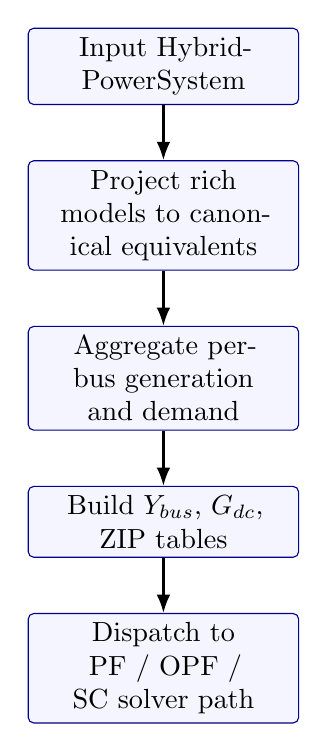
\begin{tikzpicture}[node distance=7mm and 10mm]
  \node[flowbox] (start) {Input \texttt{HybridPowerSystem}};
  \node[flowbox, below=of start] (proj) {Project rich models to canonical equivalents};
  \node[flowbox, below=of proj] (agg) {Aggregate per-bus generation and demand};
  \node[flowbox, below=of agg] (mat) {Build \(Y_{bus}\), \(G_{dc}\), ZIP tables};
  \node[flowbox, below=of mat] (dispatch) {Dispatch to PF / OPF / SC solver path};
  \draw[flowline] (start) -- (proj);
  \draw[flowline] (proj) -- (agg);
  \draw[flowline] (agg) -- (mat);
  \draw[flowline] (mat) -- (dispatch);
\end{tikzpicture}
\caption{Shared preprocessing path used by the main PF, native OPF, parity OPF, and SC modules.}
\end{figure}

\subsection{Hybrid Newton Power Flow}

\begin{figure}[H]
\centering
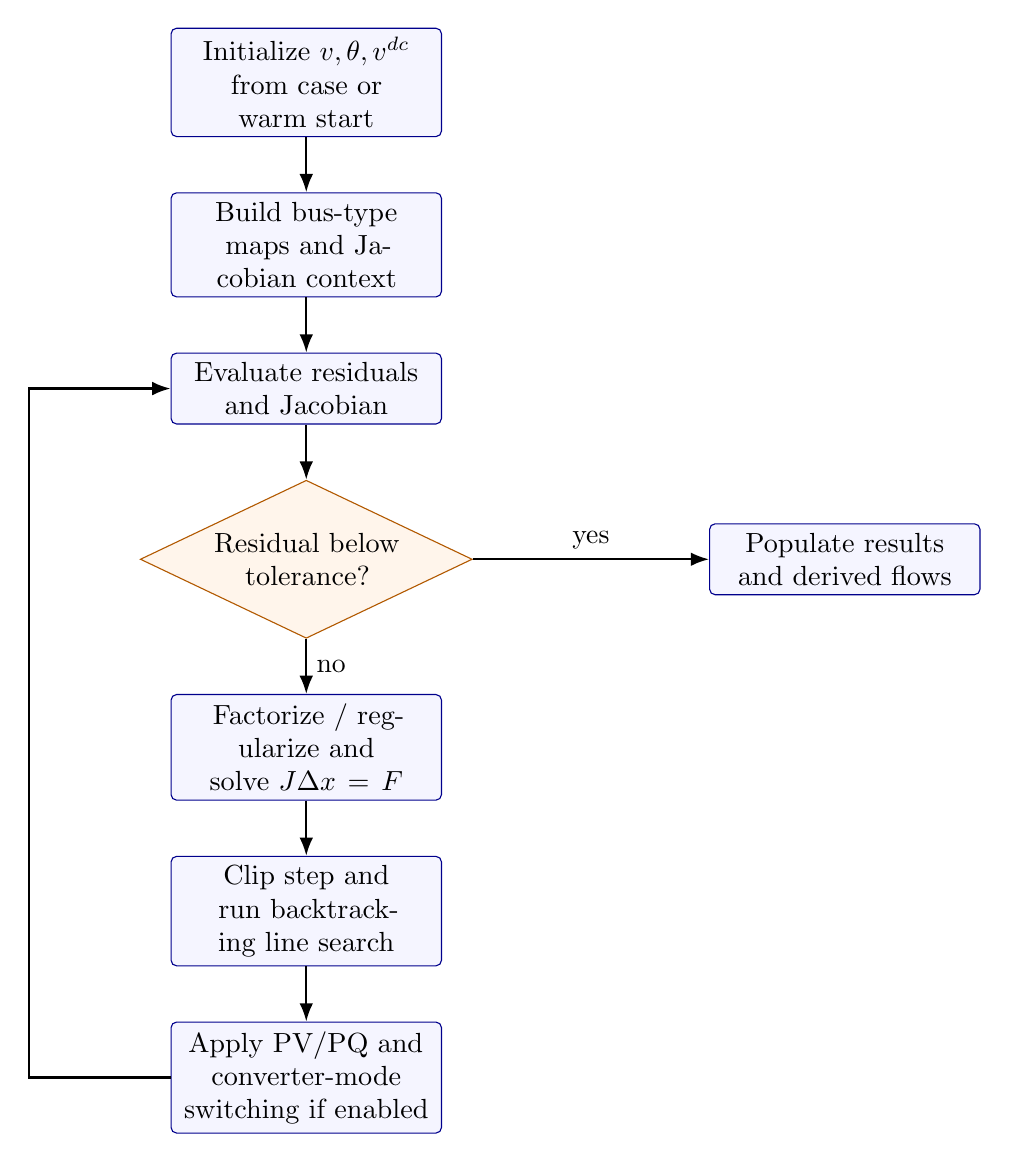
\begin{tikzpicture}[node distance=7mm and 12mm]
  \node[flowbox] (init) {Initialize \(v,\theta,v^{dc}\) from case or warm start};
  \node[flowbox, below=of init] (ctx) {Build bus-type maps and Jacobian context};
  \node[flowbox, below=of ctx] (eval) {Evaluate residuals and Jacobian};
  \node[decision, below=of eval] (conv) {Residual below tolerance?};
  \node[flowbox, right=30mm of conv] (done) {Populate results and derived flows};
  \node[flowbox, below=of conv] (linsolve) {Factorize / regularize and solve \(J\Delta x = F\)};
  \node[flowbox, below=of linsolve] (clip) {Clip step and run backtracking line search};
  \node[flowbox, below=of clip] (switch) {Apply PV/PQ and converter-mode switching if enabled};
  \draw[flowline] (init) -- (ctx);
  \draw[flowline] (ctx) -- (eval);
  \draw[flowline] (eval) -- (conv);
  \draw[flowline] (conv) -- node[above]{yes} (done);
  \draw[flowline] (conv) -- node[right]{no} (linsolve);
  \draw[flowline] (linsolve) -- (clip);
  \draw[flowline] (clip) -- (switch);
  \draw[flowline] (switch.west) |- ++(-18mm,0) |- (eval.west);
\end{tikzpicture}
\caption{Main Newton-Raphson workflow for hybrid AC/DC power flow.}
\end{figure}

\subsection{AC OPF Path Selection}

\begin{figure}[H]
\centering
\resizebox{\linewidth}{!}{%
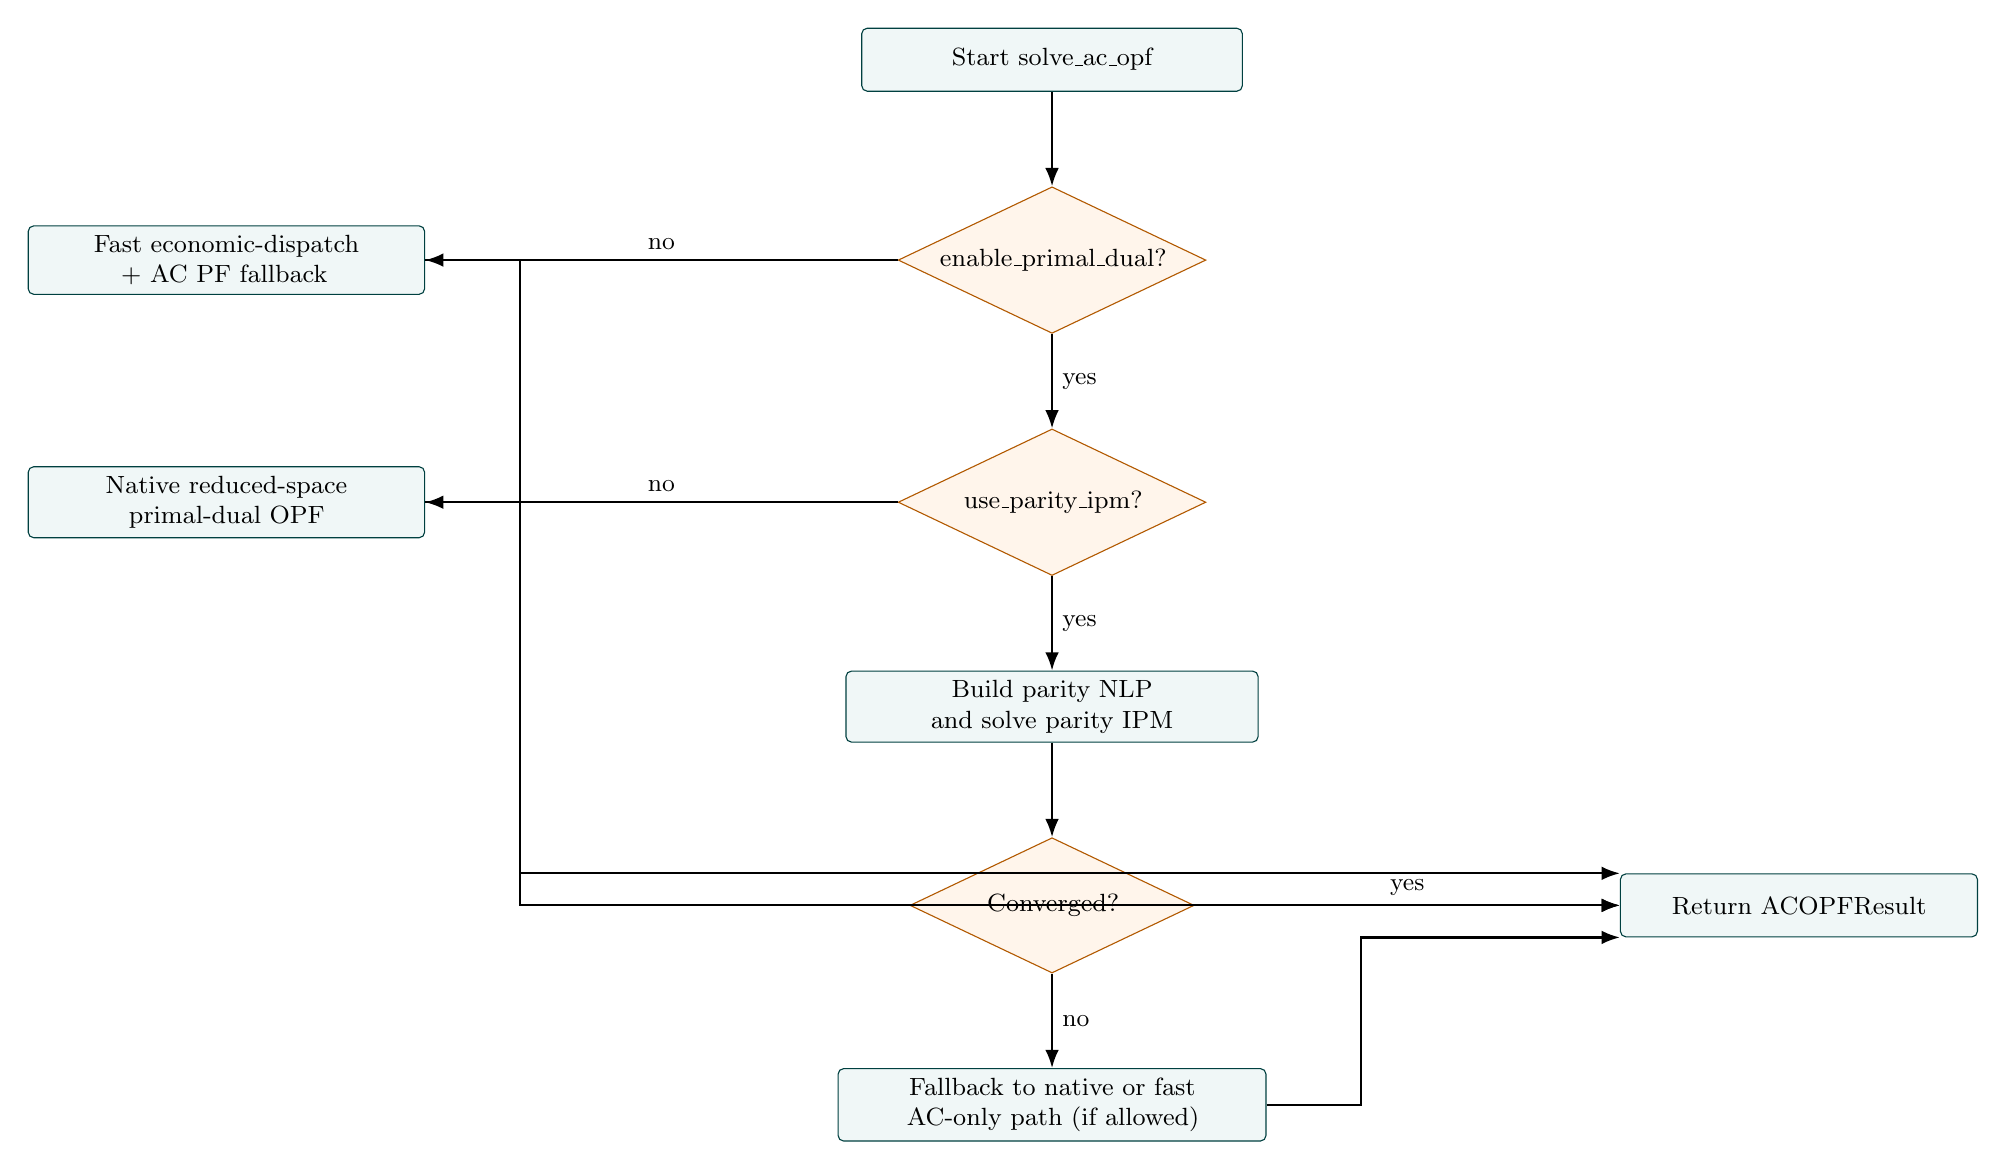
\begin{tikzpicture}[
  node distance=12mm and 22mm,
  every node/.style={font=\small}
]
  \node[flowwide] (start) {Start \texttt{solve\_ac\_opf}};
  \node[decision, below=of start, text width=3.1cm] (pd) {\texttt{enable\_primal\_dual}?};
  \node[flowwide, left=60mm of pd, text width=4.8cm] (fast) {Fast economic-dispatch + AC PF fallback};
  \node[decision, below=of pd, text width=3.1cm] (parity) {\texttt{use\_parity\_ipm}?};
  \node[flowwide, left=60mm of parity, text width=4.8cm] (native) {Native reduced-space primal-dual OPF};
  \node[flowwide, below=of parity, text width=5.0cm] (parsolve) {Build parity NLP and solve parity IPM};
  \node[decision, below=of parsolve, text width=2.8cm] (ok) {Converged?};
  \node[flowwide, below=of ok, text width=5.2cm] (fallback) {Fallback to native or fast AC-only path (if allowed)};
  \node[flowwide, right=54mm of ok, text width=4.3cm] (done) {Return \texttt{ACOPFResult}};
  \draw[flowline] (start) -- (pd);
  \draw[flowline] (pd) -- node[above]{no} (fast);
  \draw[flowline] (pd) -- node[right]{yes} (parity);
  \draw[flowline] (parity) -- node[above]{no} (native);
  \draw[flowline] (parity) -- node[right]{yes} (parsolve);
  \draw[flowline] (parsolve) -- (ok);
  \draw[flowline] (ok) -- node[above]{yes} (done);
  \draw[flowline] (ok) -- node[right]{no} (fallback);
  \draw[flowline] (fast.east) -- ++(12mm,0) |- (done.north west);
  \draw[flowline] (native.east) -- ++(12mm,0) |- (done.west);
  \draw[flowline] (fallback.east) -- ++(12mm,0) |- (done.south west);
\end{tikzpicture}
}
\caption{Current top-level solver-selection logic for AC OPF.}
\end{figure}

\subsection{Hybrid Carbon-Analysis Workflow}

\begin{figure}[H]
\centering
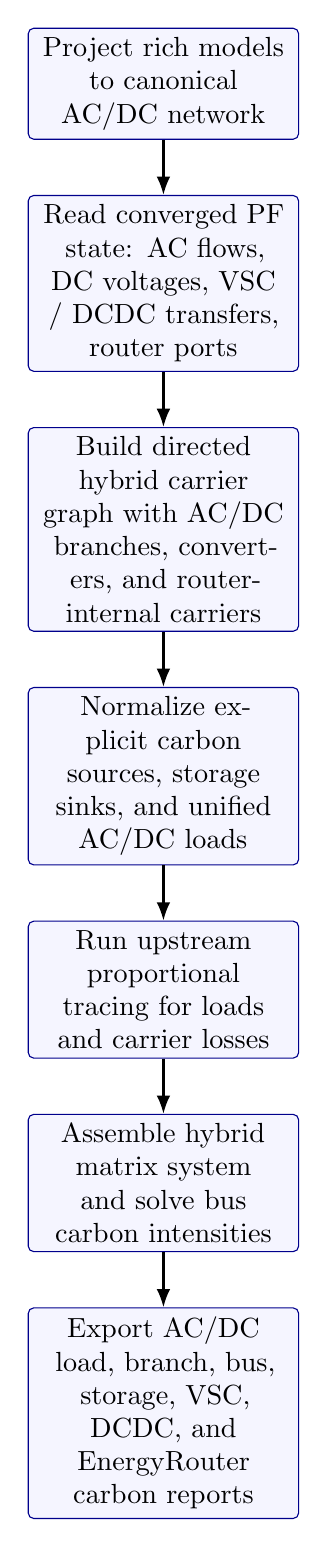
\begin{tikzpicture}[node distance=7mm and 12mm]
  \node[flowbox] (proj) {Project rich models to canonical AC/DC network};
  \node[flowbox, below=of proj] (pf) {Read converged PF state: AC flows, DC voltages, VSC / DCDC transfers, router ports};
  \node[flowbox, below=of pf] (graph) {Build directed hybrid carrier graph with AC/DC branches, converters, and router-internal carriers};
  \node[flowbox, below=of graph] (norm) {Normalize explicit carbon sources, storage sinks, and unified AC/DC loads};
  \node[flowbox, below=of norm] (trace) {Run upstream proportional tracing for loads and carrier losses};
  \node[flowbox, below=of trace] (matrix) {Assemble hybrid matrix system and solve bus carbon intensities};
  \node[flowbox, below=of matrix] (report) {Export AC/DC load, branch, bus, storage, VSC, DCDC, and EnergyRouter carbon reports};
  \draw[flowline] (proj) -- (pf);
  \draw[flowline] (pf) -- (graph);
  \draw[flowline] (graph) -- (norm);
  \draw[flowline] (norm) -- (trace);
  \draw[flowline] (trace) -- (matrix);
  \draw[flowline] (matrix) -- (report);
\end{tikzpicture}
\caption{Current hybrid carbon-analysis workflow.}
\end{figure}

\subsection{Distribution PF Workflow}

\begin{figure}[H]
\centering
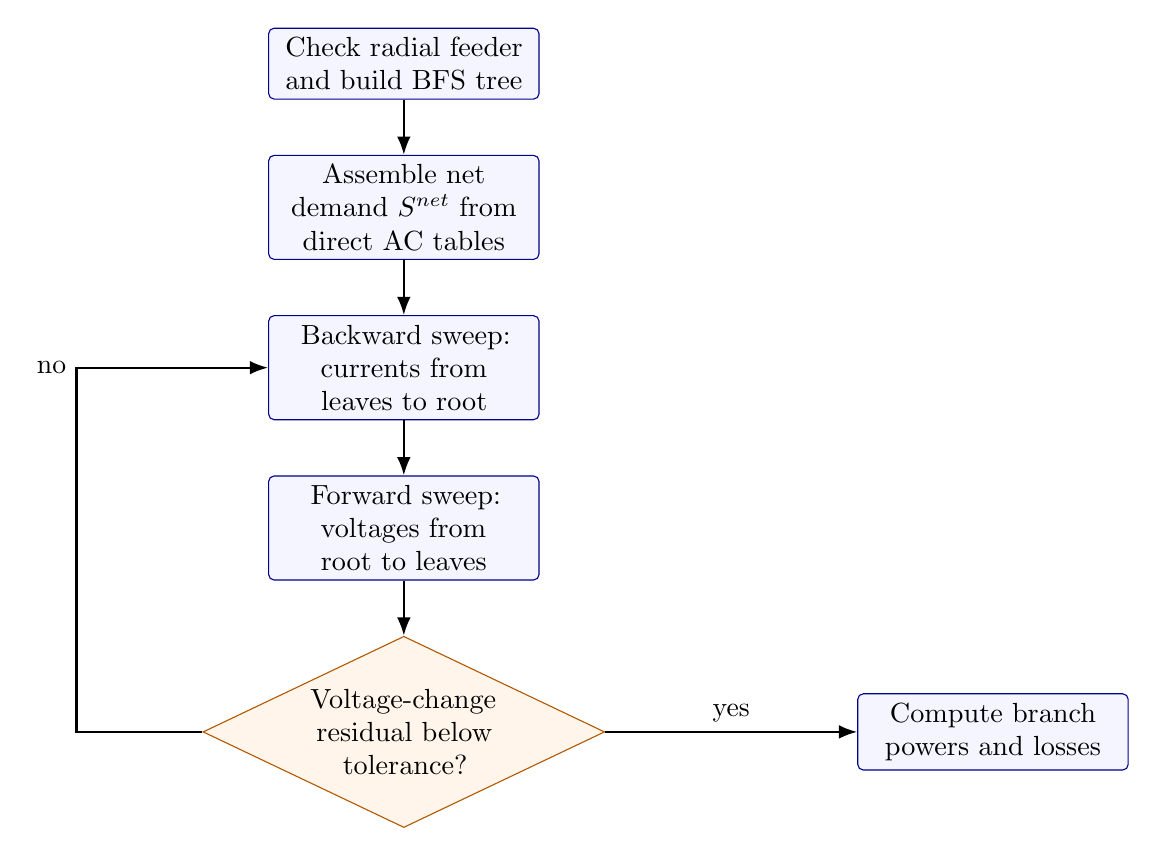
\begin{tikzpicture}[node distance=7mm and 12mm]
  \node[flowbox] (tree) {Check radial feeder and build BFS tree};
  \node[flowbox, below=of tree] (inj) {Assemble net demand \(S^{net}\) from direct AC tables};
  \node[flowbox, below=of inj] (back) {Backward sweep: currents from leaves to root};
  \node[flowbox, below=of back] (forw) {Forward sweep: voltages from root to leaves};
  \node[decision, below=of forw] (res) {Voltage-change residual below tolerance?};
  \node[flowbox, right=32mm of res] (report) {Compute branch powers and losses};
  \draw[flowline] (tree) -- (inj);
  \draw[flowline] (inj) -- (back);
  \draw[flowline] (back) -- (forw);
  \draw[flowline] (forw) -- (res);
  \draw[flowline] (res) -- node[above]{yes} (report);
  \draw[flowline] (res.west) -- ++(-16mm,0) |- node[left]{no} (back.west);
\end{tikzpicture}
\caption{Backward-forward sweep workflow for radial distribution PF.}
\end{figure}

\subsection{Short-Circuit Workflow}

\begin{figure}[H]
\centering
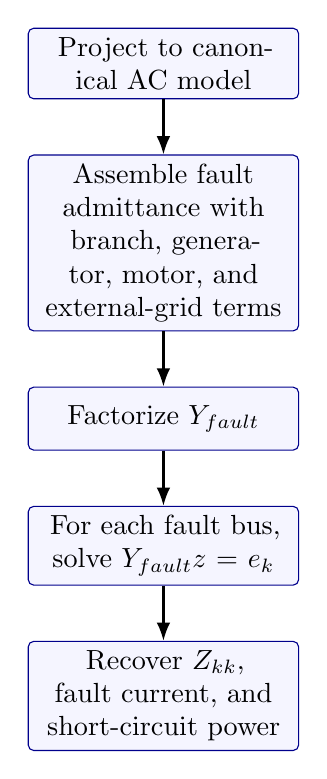
\begin{tikzpicture}[node distance=7mm and 12mm]
  \node[flowbox] (proj) {Project to canonical AC model};
  \node[flowbox, below=of proj] (ybus) {Assemble fault admittance with branch, generator, motor, and external-grid terms};
  \node[flowbox, below=of ybus] (fact) {Factorize \(Y_{fault}\)};
  \node[flowbox, below=of fact] (solve) {For each fault bus, solve \(Y_{fault}z=e_k\)};
  \node[flowbox, below=of solve] (calc) {Recover \(Z_{kk}\), fault current, and short-circuit power};
  \draw[flowline] (proj) -- (ybus);
  \draw[flowline] (ybus) -- (fact);
  \draw[flowline] (fact) -- (solve);
  \draw[flowline] (solve) -- (calc);
\end{tikzpicture}
\caption{Primary short-circuit computation path in the current module.}
\end{figure}

\subsection{ONR Workflow}

\begin{figure}[H]
\centering
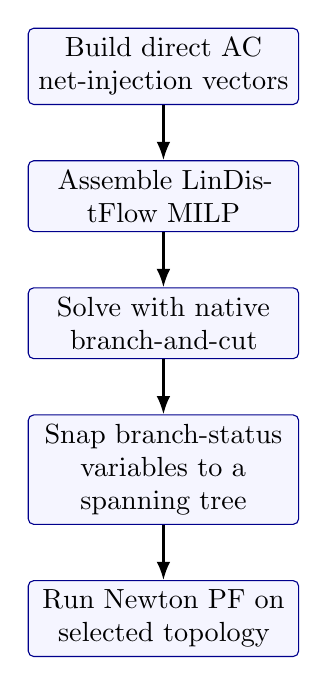
\begin{tikzpicture}[node distance=7mm and 12mm]
  \node[flowbox] (net) {Build direct AC net-injection vectors};
  \node[flowbox, below=of net] (milp) {Assemble LinDistFlow MILP};
  \node[flowbox, below=of milp] (bc) {Solve with native branch-and-cut};
  \node[flowbox, below=of bc] (snap) {Snap branch-status variables to a spanning tree};
  \node[flowbox, below=of snap] (verify) {Run Newton PF on selected topology};
  \draw[flowline] (net) -- (milp);
  \draw[flowline] (milp) -- (bc);
  \draw[flowline] (bc) -- (snap);
  \draw[flowline] (snap) -- (verify);
\end{tikzpicture}
\caption{Optimal network reconfiguration workflow.}
\end{figure}

\subsection{Solver-Family Summary}

\begin{longtable}{L{0.22\linewidth}L{0.29\linewidth}L{0.39\linewidth}}
\toprule
Workflow & Numerical core & Main reason to use it \\
\midrule
\endhead
Hybrid Newton PF & sparse Newton + line search + regularization & highest-fidelity steady-state solve in the current module. \\
DC-only PF & dense Newton on DC voltages & fast solution for purely resistive DC subnetworks. \\
FDPF & sparse decoupled angle/voltage solves & faster AC approximation when converter coupling is irrelevant. \\
Adaptive PF & island detection + per-island Newton solves & robust handling of disconnected or partially energized systems. \\
Distributed slack & post-PF mismatch redistribution & studies with multi-source slack participation. \\
Native AC OPF & custom KKT system & detailed nonlinear dispatch with direct generator/converter variables. \\
Parity OPF & parity-form NLP + dedicated IPM & full-space formulation with generator, VSC, DCDC, load-shedding, and DER decision variables; analytical Jacobian and Hessian including \(I^2R\) DCDC loss terms. \\
DC OPF & LP/QP on \(B\)-\(\theta\) network & fast linearized economic dispatch with LMP extraction; supports piecewise-linear and quadratic cost models. \\
Reactive power opt.\ (RPO) & MINLP with 4-phase OA & discrete tap/shunt optimization with AC OPF as inner NLP. \\
LCQP solver & Mehrotra predictor-corrector IPM & native convex QP/LP solver used as DC OPF backbone and RPO sub-solver. \\
Dual simplex & two-phase simplex with basis caching & LP for DC OPF and branch-and-cut MILP sub-problems; warm-start support. \\
Hybrid carbon analysis & graph tracing + dense QR on hybrid carrier graph & post-PF carbon propagation across AC branches, DC branches, storage charge/discharge states, VSC links, DCDC links, and EnergyRouter carriers. \\
BFS DPF & tree-based current/voltage sweep & radial feeder studies where a full Jacobian solve is unnecessary. \\
ONR branch-and-cut & MILP B\&C with MIR cuts & topology optimization over switch states. \\
Z-bus SC & sparse factorization of fault admittance & per-bus fault-level studies on the canonical AC model. \\
Annual production sim & hierarchical L0/L2/L3 decomposition & year-ahead scheduling with UC + OPF/PF replay. \\
Lifecycle simulation & multi-year degradation + stratified carbon & techno-economic planning with battery replacement and error bounds. \\
\bottomrule
\end{longtable}

\subsection{Code-Aligned Pseudocode (All Primary Algorithms)}
\label{sec:algo-pseudocode}

\paragraph{Algorithm A0: Runtime API Dispatch}
\begin{algorithmic}[1]
\Procedure{\texttt{run\_module}}{$sys, task, opt$}
  \If{$task=\texttt{"power\_flow"}$}
    \State \Return \texttt{solve\_power\_flow}$(sys, opt.pf)$
  \ElsIf{$task=\texttt{"dc\_power\_flow"}$}
    \State \Return \texttt{solve\_dc\_power\_flow}$(sys, opt.pf)$
  \ElsIf{$task=\texttt{"power\_flow\_adaptive"}$}
    \State \Return \texttt{solve\_power\_flow\_adaptive}$(sys, opt.pf)$
  \ElsIf{$task=\texttt{"opf"}$}
    \State \Return \texttt{solve\_ac\_opf}$(sys, opt.opf)$
  \ElsIf{$task=\texttt{"short\_circuit"}$}
    \State \Return \texttt{compute\_short\_circuit}$(sys, opt.sc)$
  \ElsIf{$task=\texttt{"network\_reconfiguration"}$}
    \State \Return \texttt{solve\_optimal\_reconfiguration}$(sys, opt.onr)$
  \ElsIf{$task=\texttt{"distribution\_pf"}$}
    \State \Return \texttt{solve\_distribution\_pf}$(sys, opt.dpf)$
  \ElsIf{$task=\texttt{"carbon\_analysis"}$}
    \State $pf \gets \texttt{solve\_power\_flow}(sys, opt.pf)$
    \State \Return \texttt{compute\_carbon\_analysis}$(sys, pf, opt.carbon)$
  \Else
    \State \Return \texttt{UnsupportedTask}
  \EndIf
\EndProcedure
\end{algorithmic}

\paragraph{Algorithm A1: Canonical Projection + SolverData Build}
\begin{algorithmic}[1]
\Procedure{\texttt{make\_solver\_data}}{$sys, loss\_model$}
  \State $projected \gets \texttt{project\_to\_canonical\_models}(sys)$
  \Statex \Comment{Includes rich-model expansion and optional zero-\(Z\) bus merging}
  \State $data \gets$ copy canonical tables from $projected$
  \State $data.loss\_model \gets loss\_model$
  \State Apply external-grid voltage/slack settings
  \State Aggregate generation and demand
  \State Build \(Y_{bus}\), \(G_{dc}\), and ZIP tables
  \State \Return $data$
\EndProcedure
\end{algorithmic}

\paragraph{Algorithm A2: \texttt{solve\_power\_flow} (Top Level)}
\begin{algorithmic}[1]
\Procedure{\texttt{solve\_power\_flow}}{$sys, opt$}
  \State $data \gets$ cached \texttt{SolverData} for $(sys, opt.loss\_model)$
  \State Apply ZIP option weights to $data$
  \State $result \gets \texttt{NewtonSolver.solve}(data, opt)$
  \State Populate branch/converter/DCDC/router derived results
  \If{$data.bus\_merge\_map$ exists}
    \State Unproject \(v_m,\theta\) back to the original AC-bus count
  \EndIf
  \State \Return $result$
\EndProcedure
\end{algorithmic}

\paragraph{Algorithm A3: Hybrid Newton PF Core}
\begin{algorithmic}[1]
\Procedure{\texttt{NewtonSolver.solve}}{$data, opt, init$}
  \State Initialize \(v,\theta,v^{\qual{dc}}\), slack sets, and control modes
  \For{$outer=1$ to \texttt{max\_outer}}
    \State Build Jacobian context and sparse pattern caches
    \For{$iter=1$ to \texttt{opt.max\_iter}}
      \State Evaluate residual and Jacobian
      \If{$\|F\|_{\infty} < \texttt{tol}$} \State \textbf{break} \EndIf
      \State Solve \(J\Delta x = F\) with regularization fallback
      \State Clip step, then run backtracking line search
      \If{no acceptable step} \State mark failure; \textbf{break} \EndIf
      \State Update state with accepted step
      \State Apply PV\(\rightarrow\)PQ and converter-mode switching rules
    \EndFor
    \If{converged and PQ\(\rightarrow\)PV restoration is enabled}
      \State Restore eligible PV buses and continue outer loop
    \Else
      \State \textbf{break}
    \EndIf
  \EndFor
  \State Export \(v,\theta,v^{\qual{dc}}\), residual, and status
  \State \Return result
\EndProcedure
\end{algorithmic}

\paragraph{Algorithm A4: DC-Only Newton PF}
\begin{algorithmic}[1]
\Procedure{\texttt{DCSolver.solve}}{$data, opt, init$}
  \State Initialize \(v^{\qual{dc}}\), detect DC slack, build reduced index set
  \For{$iter=1$ to \texttt{max\_iter}}
    \State Assemble \(P^{\qual{dc,spec}}\) from bus/load/storage/gen/VSC/DCDC/router
    \State Compute \(P^{\qual{dc,calc}} = v^{\qual{dc}} \odot (G_{dc}v^{\qual{dc}})\)
    \State Form mismatch on non-slack rows
    \If{$\|mismatch\|_{\infty} < \texttt{tol}$} \State converged; \textbf{break} \EndIf
    \State Build dense reduced Jacobian and solve for \(\Delta v^{\qual{dc}}\)
    \State Apply positivity-safe line search
  \EndFor
  \State \Return \(v^{\qual{dc}}\), residual, convergence flag
\EndProcedure
\end{algorithmic}

\paragraph{Algorithm A5: Fast-Decoupled PF (FDPF)}
\begin{algorithmic}[1]
\Procedure{\texttt{FDPFSolver.solve}}{$data, opt$}
  \State Build reduced \(B'\) and \(B''\); factorize once
  \State Initialize \(v,\theta\)
  \For{$iter=1$ to \texttt{max\_iter}}
    \State Compute \((P^{\qual{calc}},Q^{\qual{calc}})\) and ZIP-adjusted specs
    \State Form \(P\)- and \(Q\)-mismatch vectors
    \If{both mismatch norms \(<\texttt{tol}\)} \State converged; \textbf{break} \EndIf
    \State Solve \(B' \Delta\theta = -\Delta P\), \(B''\Delta v = -\Delta Q\)
    \State Update non-slack \(\theta\) and PQ-bus \(v\)
  \EndFor
  \State \Return \(v,\theta\), residual, convergence flag
\EndProcedure
\end{algorithmic}

\paragraph{Algorithm A6: Adaptive/Islanded PF}
\begin{algorithmic}[1]
\Procedure{\texttt{AdaptiveSolver.solve}}{$sys, opt$}
  \State $islands \gets \texttt{detect\_islands}(sys)$
  \If{$islands$ is empty}
    \State Solve full system once with Newton PF and return
  \EndIf
  \State Initialize global output vectors
  \For{each island}
    \If{island has no generation}
      \State Set island voltages to zero and continue
    \EndIf
    \State Auto-select swing bus if required
    \State Extract subsystem and run Newton PF (with one flat-start retry)
    \State Unproject merged AC results if bus merging occurred
    \State Map local results back to global vectors
  \EndFor
  \State Aggregate iteration count and residual
  \State \Return global adaptive result
\EndProcedure
\end{algorithmic}

\paragraph{Algorithm A7: Distributed Slack}
\begin{algorithmic}[1]
\Procedure{\texttt{solve\_distributed\_slack}}{$sys, slack\_cfg, opt$}
  \State Build/validate participation configuration
  \State Solve base PF
  \If{base PF not converged} \State \Return base result \EndIf
  \State Compute total active-power mismatch at participating buses
  \State Allocate mismatch by participation factors and optional limits
  \State Apply allocation and export adjusted injections/summary
  \State \Return distributed-slack result
\EndProcedure
\end{algorithmic}

\paragraph{Algorithm A8: AC OPF Top-Level Router}
\begin{algorithmic}[1]
\Procedure{\texttt{solve\_ac\_opf}}{$sys, opt$}
  \State Normalize default options
  \State Detect hybrid case (\(DC\) buses or VSC converters present)
  \If{hybrid case and \texttt{enable\_primal\_dual=false}}
    \State Force \texttt{enable\_primal\_dual=true}, \texttt{use\_parity\_ipm=true}
  \EndIf
  \If{\texttt{enable\_primal\_dual=true} and \texttt{use\_parity\_ipm=true}}
    \State Solve parity IPM path
    \If{failed and \texttt{allow\_fallback}} \State retry native path \EndIf
    \State \Return result
  \EndIf
  \If{\texttt{enable\_primal\_dual=false}}
    \State \Return fast dispatch + AC PF fallback path
  \EndIf
  \State \Return native primal-dual OPF path
\EndProcedure
\end{algorithmic}

\paragraph{Algorithm A9: Fast Dispatch + AC PF Fallback (OPF)}
\begin{algorithmic}[1]
\Procedure{\texttt{try\_dispatch\_pf\_fallback}}{$ac\_sys, opt$}
  \State Try direct PF projection using current generator settings
  \If{PF converged}
    \State Back-calculate bus injections and split by generator limits
    \State Compute objective and return converged OPF result
  \EndIf
  \State Solve clipped economic dispatch (\(\lambda\)-search)
  \State Rerun AC PF projection with dispatched \(P_g\)
  \If{PF converged} \State \Return converged result \EndIf
  \State \Return not-converged result
\EndProcedure
\end{algorithmic}

\paragraph{Algorithm A10: Native Primal-Dual AC/DC OPF}
\begin{algorithmic}[1]
\Procedure{\texttt{solve\_native\_primal\_dual}}{$sys, opt$}
  \State Build \(x\)-map, bounds, initial interior point, and sparse workspaces
  \For{$outer=1$ to \texttt{max\_outer}}
    \For{$inner=1$ to \texttt{max\_inner}}
      \State Unpack \(x \rightarrow (v,\theta,v^{\qual{dc}},P_g,Q_g,P^{\qual{conv,ac}},Q^{\qual{conv,ac}},P^{\qual{conv,dc}})\)
      \State Evaluate equality constraints and Jacobian
      \State Evaluate objective gradient and diagonal Hessian terms
      \State Add bound barriers and nonlinear limit penalties
      \State Solve regularized KKT step
      \State Globalize by line search/restoration
      \If{acceptance fails} \State mark failure; \textbf{break} \EndIf
      \State Update interior point and penalties
      \If{primal/dual residuals below tolerance} \State converged; \textbf{break} \EndIf
    \EndFor
    \If{converged} \State \textbf{break} \EndIf
    \State Update barrier/penalty schedule
  \EndFor
  \If{failed and fallback allowed} \State call fast dispatch fallback \EndIf
  \State \Return OPF result
\EndProcedure
\end{algorithmic}

\paragraph{Algorithm A11: Parity NLP Build + Primal-Dual IPM}
\begin{algorithmic}[1]
\Procedure{\texttt{solve\_with\_parity\_ipm}}{$sys, opt$}
  \State Build full-space parity problem (AC, DC, converters, DER, shedding)
  \State Build bounds/scaling and initial point
  \State Initialize slacks/multipliers (\(z>0,\mu>0\))
  \For{$iter=1$ to \texttt{max\_iter}}
    \State Form condensed KKT (Mehrotra predictor-corrector)
    \State Solve affine predictor, then centering-corrector steps
    \State Optionally run Gondzio extra corrections
    \State Apply fraction-to-boundary step lengths
    \State Update \(x,\lambda,z,\mu\); re-evaluate residual metrics
    \State Track best iterate
    \If{primal, dual, and complementarity tolerances met}
      \State converged; \textbf{break}
    \EndIf
  \EndFor
  \State Restore best iterate when configured and needed
  \State Map \(x\) to \texttt{ACOPFResult} fields and return
\EndProcedure
\end{algorithmic}

\paragraph{Algorithm A12: Short-Circuit (All-Bus IEC-Style)}
\begin{algorithmic}[1]
\Procedure{\texttt{compute\_short\_circuit}}{$sys, sc\_opt$}
  \State Project to canonical AC model
  \State Build/factorize fault admittance matrix once
  \For{each faulted bus \(k\)}
    \State Solve \(Y^{\qual{fault}}z=e_k\), recover \(Z_{kk}\)
    \State Apply fault type and voltage-factor rule
    \State Compute \(I_{k}^{\prime\prime}\), short-circuit power, and \(R/X\)
    \State Append per-bus detailed result row
  \EndFor
  \State \Return short-circuit result set
\EndProcedure
\end{algorithmic}

\paragraph{Algorithm A13: Optimal Network Reconfiguration (ONR)}
\begin{algorithmic}[1]
\Procedure{\texttt{solve\_optimal\_reconfiguration}}{$sys, opt$}
  \State Project rich models to canonical AC network
  \State Build bus map, root selection, and net \(P/Q\) injections
  \State Build LinDistFlow MILP with \(\alpha,P,Q,v,f,t\) variables
  \State Solve MILP using native branch-and-cut + MIR cuts
  \State Round/repair \(\alpha\) to a radial spanning tree if needed
  \State Export open/closed stable branch indices and objective
  \State Run Newton PF on selected topology for verification
  \State \Return ONR result
\EndProcedure
\end{algorithmic}

\paragraph{Algorithm A14: Distribution PF (BFS)}
\begin{algorithmic}[1]
\Procedure{\texttt{solve\_distribution\_pf}}{$system, opt$}
  \If{$system$ is \texttt{HybridPowerSystem}}
    \State Project to canonical AC system
  \Else
    \State Use provided AC system directly
  \EndIf
  \State Build bus map and BFS tree from in-service branches
  \State Assemble net demand \(S^{\qual{net}}\)
  \State Initialize complex voltage vector
  \For{$iter=1$ to \texttt{max\_iter}}
    \State Backward sweep (currents: leaves \(\rightarrow\) root)
    \State Forward sweep (voltages: root \(\rightarrow\) leaves)
    \If{max voltage update \(< \texttt{tol}\)} \State converged; \textbf{break} \EndIf
  \EndFor
  \State Compute branch powers and total losses
  \State \Return DPF result
\EndProcedure
\end{algorithmic}

\paragraph{Algorithm A15: Carbon Analysis (Tracing + Matrix)}
\begin{algorithmic}[1]
\Procedure{\texttt{compute\_carbon\_analysis}}{$sys, pf, opt$}
  \State Require converged PF state
  \State Project to canonical hybrid model and build AC/DC id maps
  \State Build unified load sinks and explicit storage carbon-source states
  \State Build directed AC/DC/converter/router flow graph
  \State Build carbon sources and reconstruct slack contribution
  \State Run proportional tracing and export per-device allocations
  \State Solve hybrid matrix carbon-intensity system for bus intensities
  \State Export summaries, balance checks, and solver-specific notes
  \State \Return carbon-analysis result
\EndProcedure
\end{algorithmic}

\paragraph{Algorithm A16: DC Optimal Power Flow}
\begin{algorithmic}[1]
\Procedure{\texttt{solve\_dc\_opf}}{$sys, opt$}
  \State Build bus/branch/generator index sets and susceptance matrix $B$
  \State Assemble cost vector (linear or quadratic depending on backend)
  \State Add per-bus load-shedding variables with auto-tuned VOLL penalty
  \State Build power-balance equality constraints (per bus)
  \State Add flow-definition equalities: $P_{f,ij} - b_{ij}(\theta_i - \theta_j) = 0$
  \State Set variable bounds ($\theta$, $P_g$, $P_f$, $\Delta P_d$)
  \State Select backend: NativeQP $\to$ Gurobi $\to$ HiGHS $\to$ Dual Simplex
  \State Solve LP or QP
  \State Extract LMPs from power-balance dual variables
  \State \Return DC OPF result with dispatch, flows, and LMPs
\EndProcedure
\end{algorithmic}

\paragraph{Algorithm A17: Reactive Power Optimization (OA)}
\begin{algorithmic}[1]
\Procedure{\texttt{solve\_reactive\_power\_opt}}{$sys, opt$}
  \State Enumerate discrete variables (transformer taps, switchable shunt steps)
  \State Solve baseline AC OPF to obtain incumbent objective
  \State \textbf{Phase 0 (Sensitivity):} For each discrete variable, perturb $\pm 1$, solve NLP, rank by $|\Delta\text{obj}|$
  \State \textbf{Phase 1 (Ternary search):} For each variable in sensitivity order, run integer ternary search; add OA cuts $f(y) \ge f_k + g_k^T(y - y_k)$ at each evaluation
  \State \textbf{Phase 2 (Coordinate descent, up to 3 cycles):} Sweep each variable; skip candidates where OA lower bound $\ge$ incumbent; add cuts; terminate if no improvement
  \State \textbf{Phase 3 (Pairwise polishing):} Check $\pm 1$ pairs of discrete variables; OA prunes before NLP evaluation
  \State \Return best tap/shunt settings, OA cuts, NLP solve count
\EndProcedure
\end{algorithmic}

\paragraph{Algorithm A18: LCQP Interior-Point Solver}
\begin{algorithmic}[1]
\Procedure{\texttt{solve\_lcqp}}{$Q, c, A_{eq}, b_{eq}, \ell, u$}
  \State Initialize $x$ at bound midpoints; $s_\ell, s_u \gets$ slacks; $z_\ell, z_u \gets 1$; $y \gets 0$
  \State Cache symbolic factorization of KKT sparsity pattern
  \For{$iter = 1$ to \texttt{max\_iter}}
    \State Compute complementarity gap $\mu = (s_\ell^T z_\ell + s_u^T z_u) / (2n_{\text{bounded}})$
    \If{primal, dual feasibility, and gap $< \epsilon$} \State converged; \textbf{break} \EndIf
    \State Form KKT residuals (stationarity, primal feasibility, complementarity)
    \State Solve predictor step via sparse LU with $\epsilon$-regularization
    \State Compute centering parameter $\sigma = \min(0.3, 100\mu)$
    \State Solve corrector step with second-order compensation
    \State Compute step lengths $\alpha_p, \alpha_d$ via fraction-to-boundary ($\tau = 0.995$)
    \State Update $(x, s_\ell, s_u, y, z_\ell, z_u)$
  \EndFor
  \State \Return $x$, objective, convergence status
\EndProcedure
\end{algorithmic}

\paragraph{Algorithm A19: Dual Simplex LP Solver}
\begin{algorithmic}[1]
\Procedure{\texttt{solve\_dual\_simplex}}{$c, A, b, \ell, u$}
  \State Convert to standard form: add slacks, surplus, artificial variables
  \State \textbf{Crash basis:} For each artificial, find original column with largest $|A_{ij}|$ and swap
  \State \textbf{Phase I:} Minimize sum of artificials
  \For{$iter = 1$ to \texttt{max\_iter}}
    \State Compute reduced costs; select entering variable (most-negative)
    \State Compute step direction and leaving variable (ratio test)
    \If{all artificials non-basic} \State Phase I complete; \textbf{break} \EndIf
    \State Pivot basis; refactorize every 15--50 iterations
  \EndFor
  \If{artificials remain in basis} \State Extract Farkas certificate; \Return infeasible \EndIf
  \State \textbf{Phase II:} Minimize original $c^T x$
  \For{$iter = 1$ to \texttt{max\_iter}}
    \State Compute reduced costs
    \If{all non-negative (dual feasible)} \State optimal; \textbf{break} \EndIf
    \State Select entering/leaving variables and pivot
  \EndFor
  \State \Return $x$, objective, basis (cached for warm-start in branch-and-cut)
\EndProcedure
\end{algorithmic}

\paragraph{Algorithm A20: Annual Production Simulation}
\begin{algorithmic}[1]
\Procedure{\texttt{solve\_annual\_production\_simulation}}{$sys, ts\_data, opts$}
  \State \textbf{L0 (Annual planning):} Build coarse monthly/weekly blocks
  \Statex \quad Generate energy budgets $\bar E_{g,k}$, SOC trajectory, maintenance flags
  \For{each block $k$}
    \State \textbf{L2 (Weekly UC):} Extract sub-horizon and solve rolling UC
    \Statex \quad Binding window: $T^{(2)}$ steps; look-ahead: $T^{\qual{la}}$ steps
    \Statex \quad Call \texttt{solve\_unit\_commitment(sub\_sys, sub\_ts, ...)}
    \If{not \texttt{skip\_replay}}
      \For{each day in block}
        \State \textbf{L3 (Daily replay):} Slice UC schedule for the day
        \State Call \texttt{solve\_time\_series\_pf(sub\_sys, ...)} for OPF/PF validation
        \State Store per-step voltages, losses, flows, costs
      \EndFor
    \Else
      \State Fill step results from UC + load profiles (no OPF/PF)
    \EndIf
  \EndFor
  \State Aggregate generator/renewable/storage annual statistics
  \Statex \quad Capacity factors, curtailment rates, cycle counts, startups
  \State \Return annual result with step/block/component summaries
\EndProcedure
\end{algorithmic}

\paragraph{Algorithm A21: Lifecycle Simulation}
\begin{algorithmic}[1]
\Procedure{\texttt{run\_lifecycle\_simulation}}{$sys, opts$}
  \For{$year = 1$ to \texttt{num\_years}}
    \State Apply load growth: $P_d^{(y)} = P_d^{(0)} (1 + r_g)^{y-1}$
    \State Apply PV derating: $P_{\max}^{(y)} = P_{\max}^{(0)} (1 - d_{PV})^{y-1}$
    \State Compute battery SOH: $\min(\text{SOH}_{\text{cal}}, \text{SOH}_{\text{cyc}})$
    \If{$\text{SOH} \le \text{SOH}_{\text{EOL}}$}
      \State Trigger replacement; reset SOH and accumulate replacement cost
    \EndIf
    \State \textbf{Tier 1:} Run annual chronological dispatch
    \State \textbf{Tier 2:} Stratified sampling into 7 operating regimes
    \Statex \quad (peak load, low renewable, high curtailment, heavy charge/discharge, normal, low load)
    \State Compute Neyman-allocated sampling error bounds
    \State Compute dispatch, sampling, and storage carbon error bounds
    \State Accumulate annual OpEx and carbon metrics
  \EndFor
  \State Compute NPV: $\sum_{y} (\text{OpEx}_y + \text{ReplaceEx}_y) / (1+r)^{y-1}$
  \State \Return lifecycle result with per-year metrics and error bounds
\EndProcedure
\end{algorithmic}

\section{Native Branch-and-Cut Solver}
\label{sec:native-branch-and-cut}

This section documents the toolbox's native branch-and-cut solver from three angles at once: mathematical model, algorithmic workflow, and code-level realization. The implementation is centered on
\texttt{include/hacdcpf/engine/branch_and_cut.hpp},
\texttt{src/engine/branch_and_cut.cpp},
\texttt{src/engine/bc\_utils.cpp},
\texttt{src/engine/bc\_branching.cpp},
\texttt{src/engine/bc\_cuts.cpp}, and
\texttt{src/engine/bc\_relaxation.cpp}, while the LP kernel relies on
\texttt{include/hacdcpf/engine/dual_simplex.hpp} and
\texttt{src/engine/dual_simplex.cpp}.
The public namespace is \texttt{hacdcpf::engine};
\texttt{include/hacdcpf/solver/branch_and_cut.hpp} re-exports the same solver for the adapter layer.

The discussion below is intentionally code-aligned. When the implementation differs from a textbook branch-and-cut design, this section follows the current C++ code rather than the idealized label.

\subsection{Scope and Code Map}

The module currently serves two problem classes:
\begin{itemize}
  \item MILP: the full branch-and-cut path with root cuts, pseudo-cost / reliability branching, cut pool, solution pool, primal heuristics, sequential tree search, and heterogeneous parallel tree search.
  \item MINLP: a lighter spatial branch-and-bound path with NLP relaxations, branching, and pruning, but without the MILP path's cut generation, cut pool, or dedicated cut worker.
\end{itemize}

The main source files are summarized in Table~\ref{tab:bc-file-map}.

\begin{table}[H]
\centering
\small
\caption{Branch-and-cut code map}
\label{tab:bc-file-map}
\begin{tabularx}{\linewidth}{L{0.32\linewidth}L{0.62\linewidth}}
\toprule
File & Main responsibility \\
\midrule
\texttt{include/hacdcpf/engine/branch_and_cut.hpp} & Public API, \texttt{BCOptions}, \texttt{BCStats}, \texttt{BCResult}, and solver enums. \\
\texttt{include/hacdcpf/engine/detail/bc\_types.hpp} & Core data structures: nodes, pseudo-costs, cut requests, LP relaxation records, and thread-side payloads. \\
\texttt{include/hacdcpf/engine/detail/bc\_pools.hpp} & Global \texttt{CutPool} and \texttt{SolutionPool}. \\
\texttt{include/hacdcpf/engine/detail/bc\_threading.hpp} & Thread-safe queues, shared incumbent, shared cut/solution pools, and atomic parallel statistics. \\
\texttt{src/engine/bc\_utils.cpp} & Objective normalization, fractional-variable detection, MILP presolve, node bound propagation, reduced-cost fixing, and row insertion. \\
\texttt{src/engine/bc\_branching.cpp} & Most-infeasible branching, pseudo-cost branching, and reliability branching probes. \\
\texttt{src/engine/bc\_cuts.cpp} & Tableau GMI/Gomory cuts, cover cuts, legacy integer-rounding cuts, and cut dispatch. \\
\texttt{src/engine/bc\_relaxation.cpp} & LP and NLP relaxation solves plus auxiliary rounding logic. \\
\texttt{src/engine/branch_and_cut.cpp} & Root strengthening, sequential B\&C, heterogeneous parallel B\&C, and MILP/MINLP top-level orchestration. \\
\texttt{src/engine/dual_simplex.cpp} & Standard-form construction, sparse and dense simplex, dual-simplex reoptimization, and incremental bound updates in standard form. \\
\bottomrule
\end{tabularx}
\end{table}

The most direct solver entry points in the current toolbox are:
\begin{itemize}
  \item \texttt{solve\_milp\_bc(prob, opt)} for MILP.
  \item \texttt{solve\_minlp\_bc(prob, opt)} for MINLP.
  \item \texttt{NativeBranchAndCutAdapter} for integration into the solver-adapter interface.
  \item \texttt{analysis/topology\_analysis.cpp} for ONR-type MILP usage.
  \item \texttt{analysis/time\_series\_pf.cpp}, \texttt{tests/test\_unit\_commitment.cpp}, and \texttt{tests/test\_uc\_performance.cpp} for UC and scheduling-style MILP integration and tuning.
\end{itemize}

\subsection{Active and Prepared Tree Data Structures}

The active MILP and MINLP solve paths still use the legacy \texttt{Node} structure:
\begin{itemize}
  \item full node bounds \texttt{lb}/\texttt{ub},
  \item relaxation solution \texttt{x\_relax},
  \item optional seed \texttt{x\_seed},
  \item simplex warm-start hint \texttt{basis\_hint},
  \item node bound \texttt{bound}, and
  \item tree depth.
\end{itemize}

A recent implementation change made \texttt{Node::branch\_child()} explicitly lightweight: it copies only bounds, basis hint, bound, and depth, but skips copying \texttt{x\_relax} and \texttt{x\_seed}. This matters because branching creates children frequently, and the solver now avoids unnecessary vector copies on the hot path.

At the same time, \texttt{bc\_types.hpp} now also contains a prepared diff-based representation:
\begin{itemize}
  \item \texttt{BoundChange},
  \item \texttt{TreeNode}, and
  \item \texttt{TreeDomainManager}.
\end{itemize}

These structures support LCA-based switching between nodes by replaying bound changes rather than copying full bound vectors. As of the current implementation, they are present in the type layer but are not yet wired into the active branch-and-cut search loop. Therefore the operational solver still uses the legacy full-bound \texttt{Node} path.

\subsection{Problem Class and Outer Mathematical Model}

For MILP, the input object is \texttt{MIPModel}, whose linear part is \texttt{LPModel}:
\begin{align}
  \min/\max \quad & c^\top x \\
  \text{s.t.}\quad & A x \le b, \\
                    & A_{eq} x = b_{eq}, \\
                    & \ell \le x \le u, \\
                    & x_j \in \mathbb{Z} \text{ or } \{0,1\}, \quad j \in \mathcal{I}.
\end{align}

The outer B\&C logic compares all bounds in a unified minimization metric. The helper
\texttt{objective\_value(c, x, sense)} returns \(c^\top x\) for minimization and
\(-c^\top x\) for maximization, so pruning, pseudo-cost updates, and gap computation can all be written as
\begin{align}
  z_{LP}(N) &\le z^\star \le z_{inc}, \\
  \text{gap} &= \max\!\left(0, \frac{z_{inc} - z_{LB}}{\max(1, |z_{inc}|)}\right).
\end{align}

For a fractional integer variable \(x_j^\ast\), the two children are
\begin{align}
  \text{down child}:\quad & x_j \le \lfloor x_j^\ast \rfloor, \\
  \text{up child}:\quad   & x_j \ge \lceil x_j^\ast \rceil.
\end{align}

A node is pruned if any of the following happens:
\begin{itemize}
  \item the node bounds are inconsistent, that is, \(\ell_i > u_i\) for some \(i\);
  \item the LP or NLP relaxation is infeasible or numerically rejected;
  \item the node bound is not better than the incumbent, that is, \(z_{LP}(N) \ge z_{inc}\);
  \item the relaxation solution is already integral, in which case it becomes a candidate incumbent immediately.
\end{itemize}

\subsection{MILP Presolve and Bound Strengthening}

\texttt{milp\_presolve()} runs before the root node is solved. It is not a general-purpose black-box presolve; it is a branch-and-cut-oriented propagation engine focused on bounds, fixings, and matrix simplification.

\paragraph{1. Inequality and equality bound tightening}
For an inequality row \(a^\top x \le b\), the code computes the minimum activity
\begin{equation}
L(a,\ell,u)=\sum_{a_j>0} a_j \ell_j + \sum_{a_j<0} a_j u_j,
\end{equation}
and then derives tighter upper or lower bounds variable by variable. Equality rows use both minimum and maximum activity, so they can be stronger. Integer and binary bounds are rounded immediately with \(\lfloor \cdot \rfloor\) or \(\lceil \cdot \rceil\).

\paragraph{2. Singleton-row processing}
If a row contains only one nonzero coefficient, it directly implies a bound on that variable. Equality singletons can fix a variable outright. Fixed singleton rows are then removed from the active matrix.

\paragraph{3. Redundant-row elimination}
If an inequality already satisfies \(\max a^\top x \le b\) under current bounds, the row is redundant and removed from \texttt{A}.

\paragraph{4. Binary probing inside presolve}
For unfixed binary variables, the presolver probes \(x_j=0\) and \(x_j=1\), applies three rounds of propagation in each branch, and then:
\begin{itemize}
  \item fixes the variable if one side is infeasible, or
  \item merges implied bounds back into the root model if both sides are feasible.
\end{itemize}

\paragraph{5. Fixed-variable substitution}
If \(\ell_j=u_j\), the contribution of that variable is absorbed into \(b\) and \(b_{eq}\), and the corresponding matrix column is zeroed out during sparse-matrix rebuild. This reduces effective LP density before simplex begins.

A lighter version of the same idea is repeated at tree nodes through
\texttt{node\_bound\_propagation()}. The node-level propagator does not rebuild matrices; it only tightens current node bounds for two or three rounds before the LP solve, which allows cheap infeasibility detection before simplex reoptimization.

\subsection{Standard Form and LP Relaxation Kernel}

LP node solves are not performed directly on
\((A,b,A_{eq},b_{eq},\ell,u)\). The solver first constructs a bounded standard form via \texttt{build\_standard\_form\_lp()}.
For each original variable, it defines
\begin{equation}
  x = \ell + y, \qquad y \ge 0,
\end{equation}
and stores finite upper bounds in \texttt{var\_ub}, that is,
\(0 \le y_j \le u_j-\ell_j\).
The resulting internal LP is represented as a maximization problem,
\begin{align}
  \max \quad & c_{max}^\top z \\
  \text{s.t.}\quad & \widetilde A z = \widetilde b, \\
                    & 0 \le z \le \widetilde u.
\end{align}

Important implementation details are:
\begin{itemize}
  \item The internal objective is always maximization, with \(c_{max}=-c_{min}\).
  \item \(\le\) rows receive slack variables; \(\ge\) rows receive surplus plus artificial variables; equality rows receive artificial variables.
  \item If a shifted right-hand side is negative, the whole row is multiplied by \(-1\), and the row sense is flipped so that the stored RHS becomes nonnegative.
  \item Finite upper bounds are kept implicitly through \texttt{var\_ub} and \texttt{at\_upper}; they are not converted into explicit rows.
\end{itemize}

So the LP kernel is closer to a bounded-form revised simplex than to the textbook lower-bound-only standard form. This is the key reason why both bounded-form GMI generation and dual-simplex warm starts are efficient in the current implementation.

\paragraph{Fast bound updates}
Most children modify only one or two bounds. For that reason,
\texttt{update\_standard\_form\_bounds()} updates only
\texttt{lb\_shift}, \texttt{b}, \texttt{var\_ub}, and \texttt{objective\_const}, without rebuilding \texttt{A}. When no more than 50 lower-bound components change, the code applies sparse column-wise incremental updates; otherwise it falls back to a full sparse matrix-vector product.

\paragraph{LP relaxation solve modes}
\texttt{solve\_lp\_relaxation()} has two front-end modes:
\begin{itemize}
  \item Default path: \texttt{use\_simplex\_lp\_nodes=true}. The solver uses the native simplex kernel and returns a basis hint, reduced costs, and optionally a persisted sparse basis object for child-node warm starts and GMI separation.
  \item Fallback path: \texttt{use\_simplex\_lp\_nodes=false}. The LP is wrapped as an NLP with zero Hessian and solved by the native IPM. This still gives a relaxation solution, but tableau-based cuts are unavailable unless a \texttt{SimplexResult} exists.
\end{itemize}

\subsection{Warm Start by Dual Simplex}

The main theoretical fact behind the tree search is simple: when branching only changes variable bounds, the constraint matrix \(A\) remains unchanged. Therefore the parent basis is often still structurally useful for the child. In bounded-form simplex, reduced costs are determined by
\begin{equation}
  \bar c = c_{max} - A^\top y, \qquad y = B^{-T} c_B,
\end{equation}
so a basis reused under changed bounds often stays dual feasible while losing primal feasibility. That is exactly the setting in which dual simplex is effective.

The implementation currently contains three practical warm-start regimes.

\paragraph{Path A: sparse warm start for large LPs}
For \(m > \texttt{kSparseSimplexThreshold} = 200\), the code prefers a sparse basis path built around \texttt{SparseBasis}. The main steps are:
\begin{itemize}
  \item reuse the parent's persisted sparse basis and reduced costs when available;
  \item validate basis indices and block artificial columns from entering;
  \item pre-clean the basis by swapping out basic artificial variables with row slacks whenever possible, which avoids false infeasibility after bound changes;
  \item recompute \(x_B\), reduced costs, objective value, and \texttt{at\_upper} status with \texttt{sparse\_full\_recompute()} or the equivalent sparse operations;
  \item if primal feasibility is violated but dual feasibility is retained, run \texttt{sparse\_dual\_simplex\_reoptimize()};
  \item if dual reoptimization fails numerically but the basis can be refactorized, fall back to sparse primal Phase II as a last warm-start rescue.
\end{itemize}

When sparse warm start succeeds, the solver persists the sparse basis again for descendants instead of computing a dense inverse.

\paragraph{Path B: dense warm start for small LPs}
For \(m \le 200\), the solver uses the dense inverse path. If a cached inverse is available, it reconstructs the basis state quickly; otherwise it recomputes the state from the basis itself. If the reconstructed state is primal infeasible but dual feasible, it calls \texttt{dual\_simplex\_reoptimize()}.

\paragraph{Path C: cold start when warm start is unavailable or rejected}
The simplex kernel still supports cold-start Phase I / Phase II solves with slack and artificial variables. For large LPs, the sparse cold-start path uses sparse primal simplex and may use a Big-M objective if crash replacement does not remove all artificials. For small LPs, the dense path uses a classic Phase I / Phase II sequence.

\paragraph{A deliberate engineering tradeoff at tree nodes}
In the main MILP tree search, \texttt{SimplexOptions.allow\_cold\_start} is set to \texttt{false}. Therefore, when a large child-node warm start fails, the code does \emph{not} attempt an expensive cold-start Phase I / Phase II solve. Instead, that node LP is marked as failed and the branch-and-cut layer prunes it.
This is a speed-first engineering choice: it reduces node cost substantially on large UC-style MILPs, but strict completeness depends on warm-start robustness. Root solves and root cut re-solves still retain cold-start capability so that the algorithm does not lose the model at the very beginning.

\paragraph{Incumbent-aware LP early cutoff}
Both sequential and parallel MILP paths provide an incumbent bound to the simplex solver. The LP kernel can then terminate early when the node's LP bound is already provably worse than the incumbent, which avoids many unnecessary pivot iterations in nodes that would be pruned anyway.

\subsection{Cut Families and Admission Rules}

The current cut module implements three distinct families.

\paragraph{1. Tableau-based Gomory / GMI cuts}
\texttt{add\_basis\_gomory\_cuts()} builds bounded-form GMI cuts from the current simplex basis. Conceptually, if row \(r\) corresponds to a basic integer variable with value \(\beta\) and fractional part
\(f_0 = \beta - \lfloor \beta \rfloor\), the code first extracts the tableau row
\begin{equation}
  \rho = e_r^\top B^{-1} A,
\end{equation}
using either a dense \(B^{-1}\) row or sparse BTRAN. It then computes bounded-form GMI coefficients for each nonbasic column, taking into account:
\begin{itemize}
  \item whether the original variable is integer or continuous,
  \item whether that variable is currently represented at its upper bound, and
  \item the shifted lower-bound representation used by the standard form.
\end{itemize}

After that, slack and surplus columns are eliminated algebraically, and the cut is mapped back to the original variable space as
\begin{equation}
  a_{cut}^\top x \le b_{cut}.
\end{equation}

Candidate GMI cuts are not inserted blindly. They are filtered by:
\begin{itemize}
  \item violation at the current LP point,
  \item efficacy \(\text{viol}/\lVert a_{cut} \rVert_2\),
  \item density cap \texttt{gmi\_max\_density},
  \item a binary-activity score that favors cuts acting on highly fractional binary support,
  \item a binary-support ratio filter, and
  \item near-parallel rejection against already selected cuts through \texttt{gmi\_max\_parallelism}.
\end{itemize}

The ranking score is
\begin{equation}
  \text{score} = \text{efficacy} \cdot \left(1 + w_{act} \cdot \text{activity}\right),
\end{equation}
where \(w_{act}\) is \texttt{gmi\_activity\_weight}.

\paragraph{2. Cover cuts}
\texttt{add\_cover\_cuts()} scans inequality rows that contain only positive coefficients on binary variables. For a cover set \(C\) with
\begin{equation}
  \sum_{j\in C} a_j > b,
\end{equation}
it generates the classical cover inequality
\begin{equation}
  \sum_{j\in C} x_j \le |C| - 1.
\end{equation}
The implementation builds the cover greedily by sorting coefficients in descending order and accumulating until the right-hand side is exceeded.

\paragraph{3. Legacy row-based integer-rounding cuts}
\texttt{add\_mir\_like\_cuts()} reads fractional right-hand sides directly from original inequality rows and builds an older integer-rounding cut from row coefficients. In the current public interface, this family is exposed primarily by \texttt{CutType::IntRounding}.

\paragraph{Actual mapping of \texttt{CutType}}
Table~\ref{tab:bc-cut-map} records the \emph{actual current code behavior}, not the ideal meaning suggested by enum names.

\begin{table}[H]
\centering
\small
\caption{Cut-type enum and current implementation mapping}
\label{tab:bc-cut-map}
\begin{tabularx}{\linewidth}{L{0.18\linewidth}L{0.28\linewidth}L{0.44\linewidth}}
\toprule
Enum value & Actual dispatch target & Notes \\
\midrule
\texttt{None} & No cuts & Baseline mode. \\
\texttt{IntRounding} & \texttt{add\_mir\_like\_cuts} & Legacy row-based integer-rounding cuts on original inequalities. \\
\texttt{MIR} & \texttt{add\_basis\_mir\_cuts} & \texttt{add\_basis\_mir\_cuts()} currently delegates directly to \texttt{add\_basis\_gomory\_cuts()}. \\
\texttt{Gomory} & \texttt{add\_basis\_gomory\_cuts} & Main tableau-based GMI/Gomory generator. \\
\texttt{Cover} & \texttt{add\_cover\_cuts} & Binary knapsack-style cover cuts. \\
\texttt{All} & Gomory $\rightarrow$ Cover & The dispatcher now skips the MIR alias in this mode to avoid duplicate tableau GMI passes. \\
\bottomrule
\end{tabularx}
\end{table}

So if an upper-layer module says it is using ``MIR cuts'' through \texttt{CutType::MIR}, the current implementation should be understood as using the tableau GMI/Gomory generator under a different enum label. The only truly row-based family currently exposed is \texttt{IntRounding}.

\subsection{Cut Pool and Solution Pool}

\paragraph{CutPool}
The global \texttt{CutPool} stores cuts that were already generated and can be cheaply re-separated later in the tree. Each pool entry keeps a dense coefficient vector, right-hand side, age, best efficacy placeholder, and norm.
Its current policy is:
\begin{itemize}
  \item duplicate rejection by cosine similarity above 0.95,
  \item age-based replacement when the pool is full, and
  \item age reset for violated cuts plus purge after \texttt{cut\_pool\_max\_age} consecutive non-violations.
\end{itemize}

\paragraph{SolutionPool}
The solution pool stores the best \(K\) feasible integer solutions and supports guided rounding. For a fractional integer variable, guided rounding uses a vote across stored solutions to choose the rounding direction. This is more structure-aware than plain \(\text{round}(x_j)\) because it reuses historically successful integer patterns.

\subsection{Branching, Node Selection, and Primal Heuristics}

\paragraph{Branch-variable selection}
The code currently supports three branching strategies:
\begin{itemize}
  \item \texttt{FirstFractional}: branch on the first fractional variable. Useful as a baseline or debugging strategy.
  \item \texttt{MostInfeasible}: pick the variable with fractional part closest to 0.5. The score is
        \(0.5 - |\text{frac}(x_j)-0.5|\).
  \item \texttt{Pseudocost}: use a product score
        \begin{equation}
          s_j = \max\!\left(f_j \bar q_j^{\downarrow}, \varepsilon\right)
                \max\!\left((1-f_j) \bar q_j^{\uparrow}, \varepsilon\right),
          \qquad f_j = x_j - \lfloor x_j \rfloor,
        \end{equation}
        where \(\bar q_j^{\downarrow}\) and \(\bar q_j^{\uparrow}\) are average pseudo-cost estimates.
\end{itemize}

When pseudo-cost branching is enabled, shallow nodes may use
\texttt{choose\_branch\_var\_reliability()} first. That routine probes unreliable candidates by solving temporary down/up child LPs, updates pseudo-costs with true gains, and only then selects the branch variable. The current implementation behaves as follows:
\begin{itemize}
  \item reliability branching is used only up to depth 10;
  \item candidates that already received root probing data require fewer additional observations;
  \item the probing budget is more aggressive at the root and lighter at deeper nodes.
\end{itemize}

\paragraph{Node selection}
The public API exposes \texttt{BestFirst}, \texttt{DepthFirst}, and \texttt{Hybrid}. The active implementation of \texttt{Hybrid} is slightly more specific than the enum name suggests:
\begin{itemize}
  \item before an incumbent exists, new nodes are pushed to DFS;
  \item after an incumbent exists, new nodes are pushed to the best-bound priority queue;
  \item however, if the DFS stack is nonempty, it is still popped before the priority queue.
\end{itemize}
So the current \texttt{Hybrid} strategy is best read as DFS-biased with best-bound backfill, not as a strict one-time DFS-to-best-first mode switch.

\paragraph{Primal heuristics used in the main solve path}
The main branch-and-cut driver currently employs the following primal heuristics:
\begin{itemize}
  \item quick rounding after the root LP,
  \item user warm-start acceptance and warm-start repair,
  \item a fix-and-solve style feasibility pump at the root,
  \item LP diving at the root,
  \item direct rounding and guided rounding at child nodes,
  \item crossover from the two best solution-pool incumbents, and
  \item a simple RINS-like heuristic in the sequential path.
\end{itemize}

The helper \texttt{try\_rounding\_heuristic()} still exists in \texttt{bc\_relaxation.cpp}, but the production MILP path in \texttt{branch\_and\_cut.cpp} now performs the main rounding logic inline.

\subsection{Root-Node Strengthening Pipeline}

In the current implementation, the root node is much more than ``solve one LP and start branching''. The actual pipeline is shown in Algorithm~BC-R1.

\paragraph{Algorithm BC-R1: Root strengthening}
\begin{algorithmic}[1]
\Procedure{RootStrengthen}{$prob, opt$}
  \State run \texttt{milp\_presolve} on the \texttt{LPModel}
  \State solve the root LP relaxation to obtain \(x_0^{LP}\), a basis hint, and the root bound
  \If{cuts are enabled}
    \For{$k=1$ to \texttt{root\_cut\_rounds}}
      \State generate up to \texttt{cuts\_per\_round} root cuts
      \If{no cut was added} \State \textbf{break} \EndIf
      \State extend the basis hint to accommodate new slack/artificial columns
      \State re-solve the cut-augmented root LP
      \If{the re-solve fails} \State roll back the added root cuts and stop root cutting \EndIf
      \If{bound improvement stalls} \State stop root cutting early \EndIf
    \EndFor
  \EndIf
  \State seed the cut pool from accepted root cuts
  \State try user warm start and warm-start repair
  \State run the feasibility-pump loop
  \State run LP diving
  \State run two-phase root probing: domain propagation, then LP probing
  \State if an incumbent exists, run reduced-cost fixing at the root
  \State push the strengthened root node into the search queue
\EndProcedure
\end{algorithmic}

Several implementation details are especially important.

\paragraph{1. Root cut re-solve basis extension}
After adding root cuts, the standard-form dimensions change. The old basis hint is therefore not directly compatible. The code explicitly rebuilds the basis index array so that:
\begin{itemize}
  \item old inequality rows keep their relative order,
  \item new cut rows are inserted between the old inequality block and the equality block,
  \item old equality rows are shifted downward, and
  \item slack, surplus, and artificial column indices are renumbered consistently.
\end{itemize}
This is one of the key robustness mechanisms behind successful root cut re-solves.

\paragraph{2. Root cut rollback and sparse-basis cleanup}
If a root cut round adds cuts but the re-solve fails, the code truncates the newly appended inequality rows and restores the pre-cut basis, root relaxation point, and root bound. Even after successful root cutting, sparse-basis pointers created during cut re-solves are cleared before the fresh base standard form is built, because they may otherwise reference already-destroyed local matrices.

\paragraph{3. Stall detection}
Root cutting stops early if the relative bound improvement falls below \(10^{-4}\) for two consecutive rounds.

\paragraph{4. Warm-start repair}
If \texttt{prob.initial\_solution} exists, the solver first clamps it to bounds and rounds integer variables. If it is not feasible, the solver can still attempt repair by fixing the integer variables to the warm-start pattern and re-solving an LP over the continuous variables.

\paragraph{5. Feasibility pump}
The current root feasibility-pump logic has two stages:
\begin{itemize}
  \item a cheap direct rounding test, and
  \item up to five iterations of ``round integer variables, fix them, re-solve the restricted LP for the continuous part''.
\end{itemize}
So the current implementation is closer to a fix-and-solve repair loop than to the more elaborate distance-minimization feasibility-pump variants found in the literature.

\paragraph{6. LP diving}
The root diving heuristic starts from the root LP solution and greedily fixes near-integral variables while repeatedly re-solving warm-started LPs. It:
\begin{itemize}
  \item is skipped when a warm start already provided an incumbent,
  \item scales its LP budget with model size,
  \item uses a time budget of at most roughly 3\% of the global time limit and no more than about 1 second,
  \item batch-fixes variables that are already very close to integrality, and
  \item tries the opposite rounding direction if the nearest-integer fix fails.
\end{itemize}

\paragraph{7. Two-phase root probing}
Root probing has two distinct phases.
\begin{itemize}
  \item Domain-propagation probing: for each eligible unfixed binary variable, test \(x_j=0\) and \(x_j=1\) by bound propagation only. If one side becomes inconsistent, fix the variable to the other side.
  \item LP probing: for the most fractional unfixed binaries, solve temporary down/up LPs. This both initializes pseudo-costs and may produce additional fixings when one side is LP-infeasible or already dominated by the incumbent.
\end{itemize}

The LP probing budget is adaptive. It is smaller for large models and smaller again when a good incumbent already exists.

\paragraph{8. Reduced-cost fixing}
If an incumbent exists, the root can use reduced costs to fix nonbasic integer variables. The current implementation computes
\begin{equation}
  \Delta = z_{inc} - z_{LP}(N),
\end{equation}
and for a nonbasic integer variable at one of its bounds, fixes it at that bound if
\begin{equation}
  |rc_j| \ge \Delta.
\end{equation}
In the present code, reduced costs are handled in the internal minimization metric and applied only to nonbasic integer variables that are already sitting at their lower or upper bound.

\subsection{Child Processing and Sequential Tree Search}

For each child node, the helper \texttt{process\_single\_child()} applies the following steps in order:
\begin{enumerate}
  \item check bound consistency;
  \item run \texttt{node\_bound\_propagation()} on the node bounds;
  \item update the standard-form bounds by \texttt{update\_standard\_form\_bounds()} without rebuilding the matrix;
  \item solve the child LP with the parent basis hint;
  \item if an incumbent exists, run reduced-cost fixing and re-check consistency;
  \item if the LP has at most 500 inequality rows, separate violated cuts from the global cut pool and re-solve the child LP with those pool cuts;
  \item if \texttt{cuts != None} and the child depth is within \texttt{max\_cut\_depth}, generate new node cuts, add them to the global cut pool, and re-solve the node on a transient cut-augmented LP;
  \item attempt direct rounding and guided rounding to search for new incumbents.
\end{enumerate}

The 500-row threshold is a pure engineering switch. Above that size, copying \texttt{LPModel}, rebuilding \texttt{StandardFormLP}, and re-solving the LP for pool separation becomes too expensive relative to the expected gain, so the implementation skips pool separation.

A second important detail is that local node cuts are handled on a transient cut-augmented LP copy. If that re-solve succeeds, the node keeps the improved bound and LP point, but the persistent basis hint is restored to the pre-cut basis. This design keeps descendants aligned with the base LP plus node bounds rather than with a private cut-augmented submodel.

The sequential main loop can be summarized as Algorithm~BC-S1.

\paragraph{Algorithm BC-S1: Sequential MILP B\&C}
\begin{algorithmic}[1]
\Procedure{SequentialBC}{$root$}
  \While{time limit not reached, node limit not reached, and queue not empty}
    \State pop the next live node \(N\)
    \If{$z_{LP}(N) \ge z_{inc}$} \State \textbf{continue} \EndIf
    \If{$x^{LP}(N)$ is integral}
      \State update incumbent and solution pool
      \State \textbf{continue}
    \EndIf
    \State choose branch variable by reliability branching or pseudo-cost branching
    \State create down and up children
    \State process both children with \texttt{process\_single\_child}
    \State push the more promising child to DFS first and the other to the global queue structure
    \State periodically run crossover and the RINS-like heuristic
    \State update live-node lower bound and global gap
    \If{relative gap is below tolerance} \State terminate \EndIf
  \EndWhile
\EndProcedure
\end{algorithmic}

In the sequential path:
\begin{itemize}
  \item crossover is attempted every 100 explored nodes;
  \item the RINS-like heuristic is attempted every 200 explored nodes;
  \item the simplex kernel receives an atomic incumbent bound so that poor nodes can be cut off early during LP reoptimization itself.
\end{itemize}

\subsection{Heterogeneous Parallel Tree Search}

The parallel MILP path is not a homogeneous ``all workers do the same thing'' implementation. It is intentionally heterogeneous:
\begin{itemize}
  \item if \texttt{opt.cuts != None} and \texttt{max\_cut\_depth > 0}, the solver runs one dedicated cut worker plus \(N-1\) explorer threads;
  \item if cuts are only allowed at the root, all threads become explorers because a cut worker would be idle.
\end{itemize}

The explorer threads are split into two roles:
\begin{itemize}
  \item \texttt{Diver}: incumbent-oriented, DFS-biased, pseudo-cost branching, and local plunging.
  \item \texttt{Prover}: bound-oriented, best-bound queue preference, reliability branching at shallow depths, and stronger focus on proving optimality.
\end{itemize}

\paragraph{Shared parallel structures}
The parallel code uses the following shared objects:
\begin{itemize}
  \item \texttt{ThreadSafeNodeQueue}: a shared queue containing both a best-bound priority queue and a DFS stack.
  \item \texttt{SharedIncumbent}: objective bound shared by atomic compare-and-swap and solution vector shared by mutex.
  \item \texttt{SharedCutPool}: a \texttt{shared\_mutex}-protected cut pool.
  \item \texttt{SharedSolutionPool}: a mutex-protected solution pool.
  \item \texttt{CutRequestQueue}: a bounded explorer-to-cut-worker request queue.
  \item \texttt{AtomicBCStats}: lock-free or low-lock parallel counters.
\end{itemize}

\paragraph{Explorer behavior}
Each explorer owns a private copy of the base standard form. This avoids repeated synchronization around LP matrix data. In addition:
\begin{itemize}
  \item a Diver maintains a thread-local DFS stack;
  \item the maximum size of that local DFS plunge is now controlled by
        \(\texttt{kLocalDfsMax} = \max(1, \texttt{opt.max\_plunge\_depth})\);
  \item when the local plunge stack is full, additional children are spilled to the shared queue;
  \item explorers still perform node LP solves, reduced-cost fixing, pool separation, rounding, and guided rounding locally.
\end{itemize}

So \texttt{max\_plunge\_depth} is no longer a dormant option: it now actively controls how aggressively Diver threads keep nodes in thread-local DFS before returning them to the shared queue.

\paragraph{Cut worker behavior}
Explorer threads do not perform expensive tableau separation themselves in the parallel path. Instead they package the current \texttt{SimplexResult}, node bounds, node depth, and LP relaxation point into a \texttt{CutRequest} and submit it non-blockingly to the cut worker.
If the request queue is full, the request is dropped. This affects cut opportunities, not solution correctness.

The cut worker then:
\begin{itemize}
  \item pops cut requests,
  \item generates cuts,
  \item inserts newly generated rows into the shared cut pool, and
  \item when idle, continues to search for incumbents via guided rounding and crossover from the shared solution pool.
\end{itemize}

\paragraph{A code-level nuance: parallel tree cutting is currently Gomory-only}
There is an important implementation asymmetry here. Root cutting and sequential child cutting both use the generic \texttt{add\_cuts()} dispatcher, so they honor the configured \texttt{CutType}. The dedicated parallel cut worker, however, currently calls \texttt{add\_basis\_gomory\_cuts()} directly. Therefore tree-level cut generation in the parallel path is effectively Gomory/GMI-only, even if the user selected \texttt{MIR}, \texttt{Cover}, or \texttt{All}. This is a real code fact and should be kept in mind when interpreting parallel runs.

\paragraph{Monitor loop}
The main thread acts as a monitor. Roughly every millisecond it checks:
\begin{itemize}
  \item wall-clock time limit,
  \item node limit,
  \item optimality gap, and
  \item whether the shared queue is empty and no explorer is still active.
\end{itemize}

The last condition is verified twice with a short sleep in between, which reduces false termination due to queue/worker races.

\subsection{MINLP Path}

\texttt{solve\_minlp\_bc()} is currently a spatial branch-and-bound rather than a full branch-and-cut engine:
\begin{itemize}
  \item the root and child relaxations are solved by \texttt{solve\_nlp\_relaxation()} through the native IPM,
  \item branching still reuses the same branch-variable selection framework and pseudo-cost table,
  \item there is no cut generation, no cut pool, no solution pool, and no heterogeneous parallel explorer/cut-worker design.
\end{itemize}

So the name ``branch-and-cut'' is fully accurate for the MILP path, but the MINLP path should currently be understood as branch-and-bound with NLP relaxations.

\subsection{Options and Statistics}

Table~\ref{tab:bc-options} summarizes the most important user-visible solver options.

\begin{table}[H]
\centering
\small
\caption{Key \texttt{BCOptions} fields}
\label{tab:bc-options}
\begin{tabularx}{\linewidth}{L{0.27\linewidth}L{0.15\linewidth}X}
\toprule
Option & Default & Purpose \\
\midrule
\texttt{max\_nodes} & 50000 & Maximum number of explored tree nodes. \\
\texttt{max\_lp\_iter} & 500 & LP/NLP iteration budget parameter used in relaxation solves. \\
\texttt{time\_limit\_sec} & 120.0 & Global wall-clock time limit. \\
\texttt{int\_tol} & \(10^{-5}\) & Integrality tolerance. \\
\texttt{gap\_tol} & \(10^{-4}\) & Relative optimality-gap tolerance. \\
\texttt{lp\_tol} & \(10^{-6}\) & LP tolerance used to derive simplex feasibility and optimality tolerances. \\
\texttt{root\_cut\_rounds} & 5 & Maximum number of root cut rounds. \\
\texttt{cuts\_per\_round} & 10 & Maximum new cuts per round or per node. \\
\texttt{max\_cut\_depth} & 0 & Tree nodes deeper than this do not generate fresh cuts. \\
\texttt{cuts} & \texttt{None} & Cut-family selection switch. \\
\texttt{branching} & \texttt{Pseudocost} & Branch-variable selection strategy. \\
\texttt{node\_sel} & \texttt{Hybrid} & Node-selection strategy. \\
\texttt{use\_simplex\_lp\_nodes} & true & Whether node LPs use the simplex path with basis reuse. \\
\texttt{use\_feasibility\_pump} & true & Whether the root feasibility-pump loop is enabled. \\
\texttt{cut\_pool\_max\_size} & 2000 & Maximum cut-pool capacity. \\
\texttt{cut\_pool\_max\_age} & 50 & Age threshold for purging stale pool cuts. \\
\texttt{solution\_pool\_size} & 10 & Number of best incumbents kept for guided rounding and crossover. \\
\texttt{num\_threads} & 1 & Thread count; values above 1 enable the heterogeneous parallel path. \\
\texttt{cut\_worker\_queue\_size} & 64 & Maximum number of pending explorer-to-cut-worker requests. \\
\texttt{max\_plunge\_depth} & 10 & Active limit on Diver thread-local DFS plunging before spillback to the shared queue. \\
\texttt{gmi\_*} & several thresholds & Controls GMI efficacy, density, near-parallel rejection, binary activity, and support filters. \\
\bottomrule
\end{tabularx}
\end{table}

\texttt{BCStats} records diagnostics about the actual search behavior, as summarized in Table~\ref{tab:bc-stats}.

\begin{table}[H]
\centering
\small
\caption{Meaning of \texttt{BCStats} fields}
\label{tab:bc-stats}
\begin{tabularx}{\linewidth}{L{0.27\linewidth}X}
\toprule
Field & Meaning \\
\midrule
\texttt{nodes\_explored} & Number of explored nodes. \\
\texttt{lp\_solves} & Total number of LP or NLP relaxation solves. \\
\texttt{cuts\_added} & Number of newly generated cuts inserted into models. \\
\texttt{best\_bound} & Current global lower bound over live nodes. \\
\texttt{best\_obj} & Current incumbent objective value. \\
\texttt{gap} & Relative MIP gap in the solver's internal minimization metric. \\
\texttt{runtime\_sec} & Total runtime. \\
\texttt{pool\_cuts\_separated} & Number of cuts reintroduced from the global cut pool. \\
\texttt{crossover\_incumbents} & Number of incumbents found by the crossover heuristic. \\
\texttt{cut\_requests\_submitted} & Number of cut requests sent from explorers to the cut worker. \\
\texttt{cut\_requests\_dropped} & Number of cut requests dropped because the queue was full. \\
\texttt{cut\_worker\_cuts} & Number of cuts generated by the dedicated cut worker. \\
\texttt{cut\_worker\_incumbents} & Number of incumbents found by the cut worker through guided rounding or crossover. \\
\texttt{status} & Solver status string, aligned with \texttt{SolveStats.status}. \\
\bottomrule
\end{tabularx}
\end{table}

\subsection{Applications, Tests, and Code-Aligned Caveats}

\paragraph{1. Current in-toolbox usage}
The native MILP branch-and-cut solver is currently used most directly in:
\begin{itemize}
  \item ONR and topology-reconfiguration workflows,
  \item UC and scheduling-style MILP integration, and
  \item performance and regression tests that compare the native implementation against external solvers.
\end{itemize}

The current UC-oriented tuning used by \texttt{analysis/time\_series\_pf.cpp} is representative:
\begin{itemize}
  \item \texttt{cuts = CutType::Gomory},
  \item \texttt{root\_cut\_rounds = 15},
  \item \texttt{cuts\_per\_round = 20},
  \item \texttt{use\_feasibility\_pump = false},
  \item \texttt{gap\_tol = 1e-3},
  \item large \texttt{max\_lp\_iter}, and
  \item parallelism up to 8 hardware threads when available.
\end{itemize}

\paragraph{2. Existing test coverage}
The current implementation is directly exercised by at least the following test groups:
\begin{itemize}
  \item \texttt{tests/test\_branch\_and\_cut.cpp} for correctness on small MILP/MINLP instances,
  \item \texttt{tests/test\_unit\_commitment.cpp} for UC-style integration and solver behavior,
  \item \texttt{tests/test\_uc\_performance.cpp} for larger UC scaling and parallel performance, and
  \item the root-cut re-solve robustness tests associated with basis extension behavior.
\end{itemize}

\paragraph{3. Important caveats for users and developers}
The current codebase contains several behaviorally important caveats.
\begin{itemize}
  \item \textbf{\texttt{CutType::MIR} is not a distinct MIR implementation.} It currently aliases the tableau GMI/Gomory generator.
  \item \textbf{\texttt{CutType::All} no longer duplicates MIR/GMI dispatch.} It now executes one tableau GMI pass plus cover cuts.
  \item \textbf{Large child-node LPs usually do not cold start.} This is a deliberate speed optimization, not a purely textbook completeness-first design.
  \item \textbf{Pool separation is intentionally skipped for larger LPs.} Once the LP is large, a second full re-solve per child becomes too expensive.
  \item \textbf{Parallel cut requests may be dropped.} This weakens cut generation opportunities but does not invalidate incumbents or bounds already proven.
  \item \textbf{The dedicated parallel cut worker is currently Gomory-only.} Parallel tree cuts therefore do not perfectly mirror the configured \texttt{CutType} semantics.
  \item \textbf{Diff-based tree management is prepared but not active.} \texttt{TreeNode} and \texttt{TreeDomainManager} exist in the type layer, but the running solver still uses the legacy full-bound \texttt{Node} representation.
\end{itemize}

\paragraph{4. Practical interpretation}
Taken together, the native branch-and-cut solver is not a minimal teaching implementation. It is an engineering-oriented MILP core that combines:
\begin{itemize}
  \item bounded-form simplex with dual-simplex warm reoptimization,
  \item an aggressively strengthened root node,
  \item several incumbent-finding heuristics,
  \item reusable cut and solution pools,
  \item sequential and heterogeneous parallel tree search, and
  \item application-driven tuning for power-system optimization models such as ONR and UC.
\end{itemize}

The most natural next algorithmic extensions, if stricter generality is desired, are a truly distinct MIR implementation, a more explicit recovery path when large-node warm starts fail, activation of diff-based tree-state management, and richer cut or parallel logic for the MINLP path.

\section{Validation Assets and Current Evidence}

\subsection{Validation Philosophy}

The current repository already contains a meaningful cross-validation suite, but
its evidence is distributed across individual test binaries rather than a single
benchmark report.  This notebook therefore documents the current validation
assets by test intent and by covered module interaction.

\subsection{Latest Release-Mode Core Snapshot}

After the recent power-flow and OPF refactors, the current release-mode evidence
set for the core notebook modules was rerun with the nine targeted binaries
listed below.  The run completed with 865 assertions and no failures.

\begin{longtable}{@{}L{0.32\linewidth}L{0.16\linewidth}L{0.42\linewidth}@{}}
\toprule
Test binary & Assertions & Main evidence added to this notebook \\
\midrule
\endhead
\texttt{test\_all\_components\_pf} & 159 & Full-component PF coverage after the \texttt{power\_flow} directory split and Jacobian-kernel refactor. \\
\texttt{test\_annual\_production\_sim} & 405 & Annual production simulation, L0/L2/L3 orchestration, and metric aggregation. \\
\texttt{test\_carbon\_analysis} & 82 & Static hybrid carbon tracing, matrix carbon intensity, and result summaries. \\
\texttt{test\_core\_modules} & 11 & Core module smoke and utility checks. \\
\texttt{test\_modeling\_toolkit} & 146 & AML/modeling-toolkit expression, bridge, and solver-facing contracts. \\
\texttt{test\_opf\_pf\_crossval} & 24 & OPF dispatch replay through PF feasibility checks. \\
\texttt{test\_powerflow\_performance} & 3 & Optimized PF kernel smoke/performance checks. \\
\texttt{test\_problem\_types} & 14 & Engine problem-type contract coverage. \\
\texttt{test\_projection\_equivalence} & 21 & Canonical projection equivalence and stable-result behavior. \\
\textbf{Total} & \textbf{865} & \textbf{All assertions passed.} \\
\bottomrule
\end{longtable}

\subsection{Cross-Validation Map}

\begin{longtable}{L{0.34\linewidth}L{0.54\linewidth}}
\toprule
Test or evidence source & What it validates \\
\midrule
\endhead
\texttt{tests/test\_opf\_pf\_crossval.cpp} & Consistency between AC OPF outputs and PF feasibility on representative AC/DC cases such as \texttt{ieee14\_acdc}, \texttt{case33bw\_acdc}, and \texttt{case33mg\_acdc}. \\
\texttt{tests/test\_ac\_opf\_jacobian\_fd.cpp} & Finite-difference verification of the native AC OPF equality Jacobian assembly. \\
\texttt{tests/test\_parity\_formulation\_fd.cpp} and \texttt{tests/test\_parity\_hessian\_fd.cpp} & Finite-difference verification of the parity formulation and its Hessian terms. \\
\texttt{tests/test\_parity\_ipm.cpp} and \texttt{tests/test\_parity\_julia.cpp} & Parity-IPM convergence and parity-path cross-checks against reference behavior. \\
\texttt{tests/test\_distribution\_pf\_crossval.cpp} & BFS-vs-Newton agreement on radial networks, plus validation of DER injections, hybrid feeder overlays, PV power curves, and stationary vs transit mobile storage behavior. \\
\texttt{tests/test\_short\_circuit\_crossval.cpp} & Analytical and self-consistency checks for short-circuit levels, Thevenin impedances, and API consistency between per-bus and batch runs. \\
\texttt{tests/test\_topology\_crossval.cpp} & Connectivity/radiality checks, 6-bus ONR comparison against exhaustive spanning-tree enumeration, and IEEE-33 style post-reconfiguration verification with Newton PF. \\
\texttt{tests/test\_solver\_handle.cpp} & Consistency between cached solver-handle runs and direct API runs. \\
\texttt{tests/test\_case\_builders.cpp}, \texttt{tests/test\_json\_roundtrip\_new\_components.cpp}, \texttt{tests/test\_excel\_comprehensive\_case.cpp} & Input-model integrity and serialization round-trip coverage for the expanded information model. \\
\texttt{tests/test\_acopf\_dcopf\_crossval.cpp} & DC OPF convergence on MATPOWER cases (IEEE 14/30/57/118/300), objective and dispatch cross-validation against AC OPF, LMP extraction, and PF feasibility check of DC OPF dispatch. \\
\texttt{tests/test\_annual\_production\_sim.cpp} & Annual production-simulation smoke tests: L0 annual planning, L2 weekly UC, L3 daily replay pipeline, and annual metric aggregation on small benchmark systems. \\
\texttt{tests/test\_lifecycle\_smoke.cpp} & Multi-year lifecycle simulation smoke tests: degradation application, stratified sampling, NPV accumulation, and year-by-year result consistency. \\
\bottomrule
\end{longtable}

\subsection{What Is Well Covered Today}

The current repository has comparatively strong evidence in the following areas.
\begin{itemize}
  \item Main PF correctness on representative AC/DC test cases.
  \item Derivative correctness for both native and parity OPF paths, including
  finite-difference verification of DCDC converter \(I^2R\) Jacobian and Hessian
  terms.
  \item VSC converter loss model consistency between PF and OPF
  (\(P_{\mathrm{loss}} = a + b\,I_{ac} + c\,I_{ac}^2\)).
  \item DCDC converter model consistency: efficiency, \(I^2R\) conduction loss,
  and correct sign-convention handling across PF and OPF solvers.
  \item OPF\(\to\)PF cross-validation on hybrid AC/DC cases, confirming
  that OPF dispatch is PF-feasible within documented tolerances.
  \item DC OPF vs AC OPF cross-validation on standard MATPOWER cases,
  confirming dispatch and objective agreement within expected DC-approximation
  error bounds, and PF feasibility of DC OPF dispatch.
  \item DPF agreement with Newton PF on radial benchmark feeders.
  \item ONR feasibility and post-solve verification through the full PF solver.
  \item Short-circuit self-consistency and small-network analytical checks.
  \item Input/output round trips for the enlarged public information model.
  \item Annual production simulation end-to-end pipeline (L0\(\to\)L2\(\to\)L3) on small benchmark systems.
  \item Lifecycle simulation multi-year degradation and NPV consistency.
\end{itemize}

\subsection{What Still Needs Better Validation}

The code structure itself highlights the most important evidence gaps.
\begin{itemize}
  \item DPF and ONR now share the canonical projection path, but the repository still lacks explicit projected-vs-canonical equivalence tests for feeders containing transformers, switches, flexible loads, asymmetric loads, and chargers.
  \item The detailed IEC short-circuit path is now exercised by dedicated tests, but stronger reference-case validation is still needed for explicit external-grid contribution accounting and richer component-by-component breakdown semantics.
  \item The parity path now instantiates richer component-variable blocks including DCDC converter dispatch with analytical Jacobian and Hessian, but the public OPF export contract still lags the in-memory result struct, so result-I/O regression tests should be extended when those fields are serialized.
  \item A direct notebook-generation regression target should eventually verify that all documented formulas still match the implementation.
  \item The reactive-power optimisation (RPO) path has no dedicated test file; convergence and OA gap properties are exercised only indirectly through internal development runs.
  \item The annual production simulation has smoke-level coverage but no reference-case comparison against an external production-cost tool.
  \item The lifecycle simulation has smoke-level coverage; stronger validation would include comparison of NPV results against manual spreadsheet calculations on a known degradation curve.
\end{itemize}

\subsection{Suggested Interpretation for Users}

At the current maturity level, the strongest production path is:
\begin{align}
\text{projected main PF / native OPF / parity OPF / DC OPF / batch+detailed SC / annual sim},
\end{align}
while DPF and ONR should still be used with awareness of their narrower hybrid
overlay coverage and their currently lighter result contracts.  This is not a
weakness of the numerical cores themselves; it is primarily an interface- and
consumer-contract issue between the rich public model layer and specialized
distribution-planning workflows.

\section{Current Project Implementation Audit}
\label{sec:current-project-audit}

\subsection{Audit Scope and Reading Order}

This section is a code-aligned snapshot of the current project state as of
May~5,~2026, after the recent refactors to the power-flow and OPF modules.  It
does not replace the detailed derivations in the individual chapters.  Instead,
it provides one consolidated ledger that connects the current mathematical
models, algorithms, implementation files, numerical evidence, and code-quality
plan for each major module.

The current filesystem convention is:
\begin{itemize}
  \item \texttt{include/hacdcpf/power\_flow} and \texttt{src/power\_flow} for steady-state PF kernels,
  \item \texttt{include/hacdcpf/optimal\_power\_flow} and \texttt{src/optimal\_power\_flow} for OPF kernels,
  \item \texttt{include/hacdcpf/engine} and \texttt{src/engine} for reusable numerical optimization machinery,
  \item \texttt{include/hacdcpf/analysis} and \texttt{src/analysis} for secondary analysis modules,
  \item \texttt{include/hacdcpf/planning} and \texttt{src/planning} for planning studies and reporting.
\end{itemize}
The C++ namespace \texttt{hacdcpf::powerflow} is intentionally unchanged; only
the source and include paths were renamed.

\subsection{Canonical Mathematical Form Shared by the Project}

Most modules are built from one canonical hybrid-system representation.  The
runtime flow is
\begin{align}
\texttt{HybridPowerSystem}
&\xrightarrow{\text{canonical projection}} \texttt{SolverData}, \\
\texttt{SolverData}
&\xrightarrow{\text{matrix / residual build}}
\text{PF, OPF, analysis, and planning kernels}.
\end{align}
The shared steady-state equations have the compact form
\begin{align}
F_{\mathrm{pf}}(x) =
\begin{bmatrix}
P^{\mathrm{spec}}_{\mathcal{N}_{ac}\setminus\mathcal{N}_{sl}}(x)-P^{\mathrm{calc}}_{\mathcal{N}_{ac}\setminus\mathcal{N}_{sl}}(v,\theta) \\
Q^{\mathrm{spec}}_{\mathcal{N}_{PQ}}(x)-Q^{\mathrm{calc}}_{\mathcal{N}_{PQ}}(v,\theta) \\
P^{\mathrm{spec}}_{\mathcal{N}_{dc}\setminus\mathcal{N}_{dc,sl}}(x)-v^{dc}\circ (G_{dc}v^{dc})
\end{bmatrix}=0,
\end{align}
with ZIP demand, VSC converter losses, DCDC efficiency and \(I^2R\) loss, energy
router ports, storage, renewable generation, VPPs, microgrids, and charging
loads folded into the specified-injection terms.  The nonlinear OPF family uses
the standard constrained form
\begin{align}
\min_x\;& f(x) \\
\mathrm{s.t.}\;& g(x)=0,\qquad h(x)\le 0,\qquad x^{\min}\le x\le x^{\max},
\end{align}
where the parity route exposes a full-space AC/DC formulation, while the native
route and fast route use specialized reduced or projected forms.  The engine
layer exposes LP, QP, NLP, MILP, and MINLP kernels that all reduce to sparse
matrix models with explicit bound, equality, and inequality blocks.

\subsection{Mathematical Model Ledger}

\begin{longtable}{@{}L{0.16\linewidth}L{0.42\linewidth}L{0.34\linewidth}@{}}
\toprule
Module & Current mathematical model & Current implementation boundary \\
\midrule
\endhead
Model and I/O & Rich hybrid component graph with AC buses, DC buses, branches, transformers, switches, VSCs, DCDCs, loads, ZIP demand, storage, renewables, VPPs, microgrids, mobile storage, energy routers, chargers, external grids, and metadata.  Canonical projection normalizes equivalent structures while retaining merge metadata. & \texttt{include/hacdcpf/model}, \texttt{src/model}, \texttt{include/hacdcpf/io}, \texttt{src/io}.  JSON, Excel, MATPOWER, OpenDSS bridge, and case builders feed the same public model. \\
Power flow & Hybrid AC/DC nonlinear equations \(F_{\mathrm{pf}}(x)=0\).  AC rows use polar \(Y_{bus}\) power injections; DC rows use \(V(GV)\); VSC rows include fixed, linear, or quadratic loss; DCDC rows include bidirectional efficiency, droop, and optional \(I^2R\) loss; ZIP loads make demand voltage-dependent. & \texttt{src/power\_flow}: \texttt{solver\_data}, \texttt{admittance\_builder}, \texttt{residual\_evaluator}, \texttt{jacobian\_builder}, \texttt{jacobian\_pattern}, \texttt{ac\_kernel}, \texttt{newton\_solver}, \texttt{fdpf\_solver}, \texttt{dc\_solver}, \texttt{helm\_solver}. \\
Optimal power flow & Nonlinear AC/DC OPF with generation cost, AC/DC balance, converter balance, voltage limits, generator bounds, branch MVA limits, converter limits, DC branch limits, load shedding, controllable renewables, storage, flexible load, and DCDC decision variables.  DC OPF uses B-\(\theta\) LP/QP approximations.  RPO is a mixed-integer tap/shunt optimization with OPF subproblem evaluations. & \texttt{src/optimal\_power\_flow}: \texttt{ac\_opf}, \texttt{dc\_opf}, \texttt{parity\_formulation}, \texttt{parity\_ipm}, \texttt{reactive\_power\_opt}. \\
Engine solvers & Generic mathematical-programming models: LP/QP/NLP/MILP/MINLP in bound/equality/inequality form.  KKT systems, barrier systems, branch-and-bound trees, cut pools, presolve/postsolve transforms, simplex bases, and sparse factorization state are explicit data structures. & \texttt{include/hacdcpf/engine}, \texttt{src/engine}, and compatibility \texttt{include/hacdcpf/solver}.  Native IPM, LP IPM, LCQP, dual simplex, branch-and-cut, PDLP/PMM-style solvers, and adapters. \\
Distribution PF & Radial distribution feeder equations with backward/forward sweep and three-phase variants.  The model tracks branch current, voltage drops, unbalance, DER injections, hybrid overlays, and optional time-series topology changes. & \texttt{include/hacdcpf/analysis/distribution\_power\_flow.hpp}, \texttt{src/analysis/distribution\_power\_flow.cpp}, plus \texttt{time\_series\_distribution}. \\
Short circuit & Z-bus/Thevenin impedance model with IEC-style correction factors and multiple fault types.  Three-phase, single-line-to-ground, line-to-line, and double-line-to-ground faults are represented through sequence-domain or equivalent impedance calculations. & \texttt{include/hacdcpf/analysis/short\_circuit.hpp}, \texttt{src/analysis/short\_circuit.cpp}. \\
Network reconfiguration & LinDistFlow-style MILP with binary branch status, radiality/connectivity constraints, voltage-drop constraints, flow limits, load-service variables, switching costs, and post-solve PF feasibility checks. & \texttt{include/hacdcpf/analysis/topology\_analysis.hpp}, \texttt{src/analysis/topology\_analysis.cpp}, native branch-and-cut engine. \\
Carbon analysis & Directed hybrid carrier graph, proportional tracing, matrix-based bus carbon-intensity solve, storage source/sink treatment, converter and branch loss allocation, and emission aggregation by source/load/carrier. & \texttt{include/hacdcpf/analysis/carbon\_analysis.hpp}, \texttt{src/analysis/carbon\_analysis.cpp}, visualization/reporting helpers. \\
Time series and annual simulation & Multi-horizon operation model: representative annual planning layer, weekly UC layer, daily replay/validation layer, PF/OPF feasibility checks, emissions and cost aggregation, degradation-aware lifecycle wrapper. & \texttt{include/hacdcpf/analysis/time\_series\_pf.hpp}, \texttt{annual\_production\_sim.hpp}, \texttt{lifecycle\_simulation.hpp}, and related \texttt{src/analysis} files. \\
Reliability, resilience, MESS & Reliability/FMEA component catalog, outage/resilience state evolution, mobile energy storage dispatch heuristics, restoration scoring, and service-restoration metrics. & \texttt{include/hacdcpf/analysis/reliability\_assessment.hpp}, \texttt{resilience\_assessment.hpp}, docs sections 14--15, tests and validation demos. \\
Planning, market, stochastic dispatch & Microgrid and hybrid AC/DC distribution planning models; market-clearing and settlement models; two-stage/stochastic dispatch and decomposition formulations with extensive notebook derivations. & \texttt{include/hacdcpf/planning}, \texttt{src/planning}, \texttt{include/hacdcpf/market}, \texttt{include/hacdcpf/decomposition}, sections 10a, 10b, 16, and 17. \\
\bottomrule
\end{longtable}

\subsection{Algorithm and Implementation Ledger}

\begin{longtable}{@{}L{0.18\linewidth}L{0.40\linewidth}L{0.34\linewidth}@{}}
\toprule
Module & Implemented algorithms & Important implementation notes \\
\midrule
\endhead
Model/I/O & Canonical projection, bus merge mapping, MATPOWER parsing, JSON/Excel round trips, canned case construction, OpenDSS snapshot adapters. & Projection is the common input boundary for PF/OPF/analysis.  Compatibility headers under \texttt{core} and \texttt{solver} remain for older includes. \\
Power flow & Sparse Newton PF, FDPF, DC-only Newton, adaptive island solve, distributed slack, HELM with sparse \(Y_{trans}\), homotopy continuation, nonlinear scaling, nonmonotone line search, LM/PTC trust-region control, Newton-Krylov/GMRES with Schur preconditioning, voltage-stability/CPF. & The AC kernel and Jacobian sparsity construction are split into \texttt{ac\_kernel.cpp} and \texttt{jacobian\_pattern.cpp}.  Shared susceptance builders now serve FDPF \(B'\) and \(B''\). \\
Optimal power flow & Fast economic dispatch plus PF projection, native primal-dual AC/DC OPF, parity full-space formulation, dedicated parity IPM with Mehrotra predictor-corrector and extra correctors, DC OPF backend dispatch, RPO OA search over taps/shunts. & The parity route is the strongest current nonlinear AC/DC OPF path.  RPO is self-contained and calls AC OPF repeatedly with a solution cache and OA lower bounds. \\
Engine solvers & Dual simplex, sparse dual simplex, LP IPM, LCQP IPM, native NLP IPM, PDLP/PMM-family solvers, branch-and-cut with presolve, cuts, conflict/domain propagation, warm starts, parallel search and sharing. & The engine is now a real in-tree optimization layer rather than a thin wrapper.  Generic native NLP IPM is improving but still lags the parity-specific OPF solver on large OPF-class NLPs. \\
Distribution PF & Backward/forward sweep, radial topology traversal, DER/load aggregation, three-phase validation, time-series feeder replay. & Cross-validation against Newton PF exists for radial cases; hybrid component projection is still the main area needing broader cases. \\
Short circuit & Batch all-bus and per-bus fault analysis, Thevenin/Zbus solve, sequence fault formulas, contribution bookkeeping. & The module is mathematically usable; stronger external-grid and reference standard cases are still needed before calling the reporting contract complete. \\
Network reconfiguration & Native MILP build, branch-and-cut solve, stable branch-id result emission, radiality/connectivity checks, post-reconfiguration Newton PF validation. & Stable branch ids are mostly solved; projected/canonical equivalence cases with nontrivial ids still need stronger assertions. \\
Carbon analysis & Hybrid graph construction, directed flow extraction from PF/OPF, proportional source/load tracing, matrix bus-intensity solve, Sankey/report output. & Current tests cover core carbon accounting; richer time-coupled storage carbon-state validation remains a useful next step. \\
Time series, annual sim, lifecycle & L0/L2/L3 hierarchy, UC/OPF/PF replay, annual metric aggregation, multi-year degradation, stratified sampling, NPV accumulation. & Smoke and contract tests exist; external reference-cost cases and spreadsheet lifecycle baselines would strengthen numerical credibility. \\
Reliability, resilience, MESS & Reliability catalog, fault/service metrics, restoration heuristics, mobile storage movement/energy constraints, validation demo reporting. & The current solver is pragmatic and demonstrative; full MILP/rolling-horizon restoration remains the intended high-fidelity upgrade path. \\
Planning, market, stochastic & Benders/progressive decomposition studies, low-carbon planning cases, market settlement and reserve products, stochastic dispatch summaries. & These chapters contain strong mathematical material; implementation coverage varies by study and should be documented per executable path as experiments mature. \\
\bottomrule
\end{longtable}

\subsection{Numerical Evidence and Performance Snapshot}

The latest release-mode regression snapshot recorded for the core notebook
evidence set is summarized below.  These are not exhaustive benchmarks; they are
the current fast-to-medium confidence gates that demonstrate the refactored
modules still execute coherently after the recent source split and directory
rename.

\begin{longtable}{@{}L{0.31\linewidth}L{0.16\linewidth}L{0.43\linewidth}@{}}
\toprule
Evidence source & Assertions & Interpretation \\
\midrule
\endhead
\texttt{test\_all\_components\_pf} & 159 & Main AC/DC PF component integration: loads, DERs, converters, storage, hybrid buses, and result assembly. \\
\texttt{test\_annual\_production\_sim} & 405 & Annual production simulation stack: L0/L2/L3 orchestration, metric aggregation, and representative operation pipeline. \\
\texttt{test\_carbon\_analysis} & 82 & Hybrid carbon tracing, matrix intensity solve, source/load aggregation, and report-contract evidence. \\
\texttt{test\_core\_modules} & 11 & Core utility and module smoke checks. \\
\texttt{test\_modeling\_toolkit} & 146 & AML/modeling-toolkit variable, expression, bridge, and solver interaction coverage. \\
\texttt{test\_opf\_pf\_crossval} & 24 & OPF dispatch replay through PF feasibility checks on representative cases. \\
\texttt{test\_powerflow\_performance} & 3 & Performance-oriented PF smoke checks for the optimized/refactored kernels. \\
\texttt{test\_problem\_types} & 14 & Engine problem-type contracts and validation paths. \\
\texttt{test\_projection\_equivalence} & 21 & Canonical projection equivalence checks. \\
\textbf{Total in this release-mode snapshot} & \textbf{865} & \textbf{All assertions passed in the last recorded run.} \\
\bottomrule
\end{longtable}

Additional numerical evidence is distributed in the detailed chapters:
\begin{itemize}
  \item Section~\ref{sec:powerflow} records the power-flow refactor performance status and the D1--D6 deduplication completion state.
  \item Section~\ref{sec:opf} records AC/DC OPF, parity IPM, DC OPF, and RPO formulations.
  \item Section~\ref{sec:engine-nlp-ipm} records structured sparse NLP/IPM and parity-OPF comparison results, including large OPF cases where the parity path remains stronger than the generic native NLP path.
  \item The 10a microgrid-planning chapter records the corrected numerical study and replay-feasibility evidence.
  \item Section~\ref{sec:stochastic-dispatch-summary} and the standalone stochastic manuscript record two-stage/stochastic dispatch verification and decomposition behavior.
\end{itemize}

\subsection{Code-Quality Investigation by Module}

\begin{longtable}{@{}L{0.17\linewidth}L{0.31\linewidth}L{0.42\linewidth}@{}}
\toprule
Module & Current quality assessment & Focused improvement plan \\
\midrule
\endhead
Model and projection & Strong public information model and useful canonical projection, but some consumer paths still rely on implicit contiguous bus ids or vector order assumptions. & Add explicit id-to-position mapping utilities, use them in replay/unprojection/export code, and add non-contiguous id regression cases. \\
I/O contracts & JSON/Excel/MATPOWER coverage is broad, but the runtime model has grown faster than some result/input dictionaries. & Close remaining DC PV/static-generator serialization gaps; extend OPF and PF result exports for new dispatch vectors; add round-trip equality tests for every new table. \\
Power flow & Numerically central and recently refactored: shared susceptance builder, split Jacobian pattern/kernel/evaluator, and robust nonlinear aids.  Main remaining risk is duplicated injection accounting across PF residual, OPF parity, and validation paths. & Keep \texttt{pf\_injection\_assembly} as the shared DC source of truth; add FD tests for every AC/DC cross derivative; add one stress case per VSC/DCDC control mode. \\
Optimal power flow & Parity path is robust and feature-rich; generic native path still has performance and globalization gaps for large NLP-class OPF.  RPO lacks dedicated tests. & Continue parity/native convergence comparison; add RPO regression tests; expose all parity result vectors in output contracts; fix DCDC directional derivative consistency if current-iterate sign and reference sign diverge. \\
Engine solvers & LP/MILP center is mature, with strong presolve, warm-start, and branch-and-cut work.  Generic NLP IPM is much improved but not yet parity-competitive on large OPF cases. & Stabilize generic IPM globalization and scaling; stratify benchmark-scale tests from fast correctness gates; add per-kernel performance baselines. \\
Distribution PF & BFS and radial workflows are usable and cross-validated on representative feeders.  Hybrid overlays and projected component views are the weaker edge. & Expand cross-validation to transformers, switches, chargers, asymmetric loads, flexible loads, and projected feeder ids. \\
Short circuit & Functional mathematical core with batch/per-bus APIs.  Reporting semantics still need richer component-source breakdown. & Add external-grid contribution bucket; compare against named IEC reference cases; lock per-fault-type expected values. \\
Network reconfiguration & Stable ids and PF post-validation are mostly in place.  Branch-id semantics under projection remain the main subtle risk. & Add projected-vs-canonical branch-id set equality tests and deliberately nontrivial branch indices. \\
Carbon analysis & Core tracing and matrix methods are covered; current model is strong for static snapshots. & Add time-coupled storage carbon-intensity state tests and OPF/PF replay consistency checks for losses. \\
Time-series, annual simulation, lifecycle & End-to-end paths exist and have meaningful smoke coverage.  They need stronger external reference cases to become benchmark-grade. & Add small reference production-cost case; add lifecycle spreadsheet baseline; validate UC initial state/startup accounting. \\
Reliability, resilience, MESS & The documents and demos give a coherent practical workflow; optimization depth is still heuristic in places. & Add MILP restoration prototype or rolling-horizon benchmark; quantify service-restoration optimality gaps on fixed toy systems. \\
Planning, market, stochastic & Mathematical documentation is extensive and several studies have numerical artifacts, but implementation maturity varies by sub-study. & For each study, maintain a code map, input contract, reproducible run command, result table, and smoke/reference test. \\
Documentation and CI & Notebook coverage is broad but historically lagged fast-changing code paths. & Build the technical notebook in release gates; include the current implementation audit; keep validation tables tied to executable tests. \\
\bottomrule
\end{longtable}

\subsection{Immediate Documentation Contract}

For future development, every new module or major refactor should update five
documentation surfaces together:
\begin{enumerate}
  \item the mathematical model section that defines variables, objective, and constraints;
  \item the algorithm section that gives code-aligned pseudocode;
  \item the implementation map that names source/header files and public APIs;
  \item the validation section that names exact tests, benchmarks, and expected outputs;
  \item the improvement-plan table that records residual code-quality risks.
\end{enumerate}
This audit section should remain the high-level index, while individual chapters
remain the detailed derivation and experiment records.
\section{Hybrid AC/DC Distribution DER Planning Under Carbon and Peak \texorpdfstring{$N{-}1$}{N-1} Reliability Constraints}

This section defines a planning model for hybrid AC/DC distribution systems with distributed photovoltaic generation, distributed battery energy storage, and converter-coupled AC/DC power exchange. The model is intended for feeder-level planning rather than transmission expansion. Its distinguishing feature is the joint treatment of annual carbon control, peak-time reliability security, and extreme-event resilience: the normal-operation layer uses weighted representative operating states, the reliability layer uses a peak-snapshot \(N{-}1\) contingency set evaluated through an FMEA-style frequency-duration model, and the resilience layer uses extreme-state \(N{-}k\) scenarios with post-fault partitioning and island support.

The linear network model follows the sign conventions and AC/DC variable semantics of Section~\ref{sec:powerflow}. In particular, bus injections are taken as positive when they inject into the network, the AC feeder is represented by a P/Q LinDistFlow model with voltage-magnitude variables, and the DC subnetwork is written using conductance-based voltage differences.

\subsection{Study Object and Assumptions}

Consider a hybrid distribution system with AC bus set \(\mathcal{N}^{ac}\), DC bus set \(\mathcal{N}^{dc}\), AC branch set \(\mathcal{E}^{ac}\), DC branch set \(\mathcal{E}^{dc}\), and voltage-source converter set \(\mathcal{E}^{vsc}\). Let \(\mathcal{N}=\mathcal{N}^{ac}\cup\mathcal{N}^{dc}\). The planning horizon is one representative year.

Normal operation is represented by a weighted set of operating snapshots \(\Omega\), with weight \(\pi_\omega\ge 0\) and equivalent duration \(\Delta_\omega\) hours, satisfying
\begin{align}
\sum_{\omega\in\Omega} \pi_\omega = 1,
\qquad
\sum_{\omega\in\Omega} \pi_\omega\Delta_\omega = 8760.
\end{align}
Among these snapshots, let \(\omega^{pk}\in\Omega\) denote the system peak snapshot used for reliability planning.

Let \(\Xi\) denote a finite library of low-probability extreme states, such as storm, wildfire, flood, or heat-driven common-mode outage conditions. Each \(\xi\in\Xi\) has scenario weight \(\varpi_\xi\ge 0\), and for each extreme state let \(\mathcal{K}_\xi\) denote the associated \(N{-}k\) contingency family induced by that event.

Reliability is enforced through a single-contingency set \(\mathcal{C}\) covering the AC/DC components to be protected under an \(N{-}1\) criterion. Only the peak snapshot is analyzed under contingencies. For each failed component \(k\in\mathcal{C}\), let \(\lambda_k\) denote annual failure frequency and let \(\tau_k\) denote the equivalent outage duration used in the peak-time FMEA approximation.

The following assumptions define the intended model scope.

\begin{assumption}[Linear hybrid network model]
The planning model uses a linearized AC/DC power-flow approximation consistent with the variable conventions in Section~\ref{sec:powerflow}. The AC feeder is assumed radial or radially operated and is represented by a P/Q LinDistFlow approximation with branch active-power, branch reactive-power, and squared-voltage variables. DC active-power flow is represented by conductance-weighted DC-voltage differences, and each AC/DC converter is treated as a lossless controllable interlinking device.
\end{assumption}

\begin{assumption}[DER-assisted voltage regulation]
Reactive support may be supplied by PV inverters, BESS inverters, AC/DC converters, and upstream substations through linear box-type capability envelopes. Hence the AC voltage profile is regulated jointly by network reinforcement and controllable DER-side reactive power rather than by substations alone.
\end{assumption}

\begin{assumption}[Hierarchical reliability screening]
The reliability architecture has two security layers. The first evaluates only the peak snapshot \(\omega^{pk}\) under \(N{-}1\) contingencies. The second evaluates extreme states \(\xi\in\Xi\) under event-induced \(N{-}k\) contingencies, where post-fault partitioning and islanded operation are allowed.
\end{assumption}

\begin{assumption}[Tree-structured partition restoration]
Under extreme states, surviving substations and selected grid-forming BESS units may energize multiple supply partitions. Each energized partition must remain radial, so the post-fault topology is a forest rooted at activated substations or activated grid-forming BESS sources.
\end{assumption}

\begin{assumption}[FMEA weighting]
Reliability impact is measured through a frequency-duration-weighted peak load curtailment functional, consistent with the deterministic FMEA logic in Section~\ref{sec:distribution-reliability-fmea}.
\end{assumption}

\begin{assumption}[Snapshot storage approximation]
The planning model is not a chronological unit-commitment problem. Storage energy limits are therefore enforced by linear snapshot energy envelopes based on effective discharge/charge durations and a prescribed pre-contingency state-of-charge factor at the peak snapshot.
\end{assumption}

\subsection{Sets, Parameters, and Planning Variables}

\subsubsection{Network and device sets}

\begin{align}
\mathcal{R}^{ac} &\subseteq \mathcal{N}^{ac} && \text{AC root or substation buses}, \\
\mathcal{R}^{dc} &\subseteq \mathcal{N}^{dc} && \text{DC root or substation buses}, \\
\mathcal{N}^{pv} &\subseteq \mathcal{N} && \text{candidate PV buses}, \\
\mathcal{N}^{bess} &\subseteq \mathcal{N} && \text{candidate BESS buses}, \\
\mathcal{N}^{gfm} &\subseteq \mathcal{N}^{bess}\cap\mathcal{N}^{ac} && \text{candidate AC-side grid-forming BESS buses}, \\
\mathcal{N}^{crit} &\subseteq \mathcal{N} && \text{critical-load buses}, \\
\delta_i^{-},\delta_i^{+} &&& \text{incoming and outgoing incident branches of bus } i.
\end{align}

For each converter \(c\in\mathcal{E}^{vsc}\), let \(i(c)\in\mathcal{N}^{ac}\) be the associated AC bus and \(k(c)\in\mathcal{N}^{dc}\) be the associated DC bus.

For each AC branch \(e=(i,j)\in\mathcal{E}^{ac}\), the branch orientation is taken from the upstream bus \(i\) to the downstream bus \(j\), consistent with a radial feeder embedding used by LinDistFlow.

\subsubsection{Planning variables}

The first-stage decision vector is
\begin{align}
x := \Big(
&\overline P_i^{pv}\big)_{i\in\mathcal{N}^{pv}},
\big(\overline P_i^{bess},\overline E_i^{bess}\big)_{i\in\mathcal{N}^{bess}},
\big(\overline S_c^{vsc}\big)_{c\in\mathcal{E}^{vsc}}, \\
&\big(\overline P_r^{sub}\big)_{r\in\mathcal{R}^{ac}\cup\mathcal{R}^{dc}},
\zeta^{CO_2},\zeta^{rel},\zeta^{ext}
\Big),
\end{align}
where the components represent PV capacity, BESS power capacity, BESS energy capacity, converter capacity, substation import capability, carbon slack, peak-reliability slack, and extreme-resilience slack.

The annualized investment cost is written as
\begin{align}
C^{inv}(x) =
&\sum_{i\in\mathcal{N}^{pv}} \widehat K_i^{pv}\overline P_i^{pv}
+ \sum_{i\in\mathcal{N}^{bess}} \left(\widehat K_i^{bp}\overline P_i^{bess} + \widehat K_i^{be}\overline E_i^{bess}\right) \\
&+ \sum_{c\in\mathcal{E}^{vsc}} \widehat K_c^{vsc}\overline S_c^{vsc}
+ \sum_{r\in\mathcal{R}^{ac}\cup\mathcal{R}^{dc}} \widehat K_r^{sub}\overline P_r^{sub}.
\label{eq:10b-investment-cost}
\end{align}

\subsection{Three-Layer Planning Model}

The planning model contains three recourse layers:
\begin{enumerate}
  \item a normal-operation layer over \(\omega\in\Omega\), used for expected operating cost and annual carbon accounting;
  \item a peak-contingency layer over \(k\in\mathcal{C}\), used for \(N{-}1\) reliability enforcement by FMEA weighting;
  \item an extreme-state resilience layer over \((\xi,\kappa)\in\Xi\times\mathcal{K}_\xi\), used for \(N{-}k\) resilience enforcement under partitioned post-fault operation. In the current code base, this layer has both a legacy heuristic restoration simulator and a new strict multi-period MIP/LinDistFlow restoration skeleton for unexpected-fault replacement.
\end{enumerate}

The complete planning problem is
\begin{align}
\min_{x,\,y,\,z} \quad
& C^{inv}(x)
+ \sum_{\omega\in\Omega} \pi_\omega Q^{nor}(x,\omega)
+ \rho_{CO_2}\zeta^{CO_2}
+ \rho_{rel}\zeta^{rel}
+ \rho_{ext}\zeta^{ext}
\label{eq:10b-master-obj}\\
\text{s.t.}\quad
& x\in\mathcal X,
\label{eq:10b-master-xset}\\
& \sum_{\omega\in\Omega} \pi_\omega G^{CO_2}(x,\omega) \le \overline E^{ann}_{CO_2} + \zeta^{CO_2},
\label{eq:10b-master-carbon}\\
& \sum_{k\in\mathcal{C}} \lambda_k\tau_k H^{pk}_k(x) \le \overline E^{pk}_{rel} + \zeta^{rel},
\label{eq:10b-master-reliability}\\
& \sum_{\xi\in\Xi} \varpi_\xi \sum_{\kappa\in\mathcal{K}_\xi} \lambda_{\xi,\kappa}\tau_{\xi,\kappa} H^{ext}_{\xi,\kappa}(x)
\le \overline E^{ext}_{rel} + \zeta^{ext},
\label{eq:10b-master-extreme}\\
& \zeta^{CO_2} \ge 0,
\qquad
\zeta^{rel} \ge 0,
\qquad
\zeta^{ext} \ge 0.
\label{eq:10b-master-slacks}
\end{align}

Here \(Q^{nor}(x,\omega)\) is normal-state operating cost, \(G^{CO_2}(x,\omega)\) is snapshot carbon contribution, \(H_k^{pk}(x)\) is peak-snapshot unsupplied energy under contingency \(k\), and \(H^{ext}_{\xi,\kappa}(x)\) is unsupplied energy under extreme state \(\xi\) and higher-order contingency \(\kappa\). The scalar \(\overline E^{ann}_{CO_2}\) is the annual carbon budget, \(\overline E^{pk}_{rel}\) is an admissible FMEA-weighted peak EENS threshold, and \(\overline E^{ext}_{rel}\) is the resilience budget for extreme-state \(N{-}k\) events.

\subsection{Normal-Operation Recourse Model}

\subsubsection{Operating variables}

For each operating snapshot \(\omega\in\Omega\), the normal-state recourse variables are
\begin{align}
y_\omega := \Big(
&f_{e,\omega}^{ac},q_{e,\omega}^{ac},u_{i,\omega}^{ac},
f_{\ell,\omega}^{dc},v_{k,\omega}^{dc},
p_{c,\omega}^{vsc},q_{c,\omega}^{vsc}, \\
&p_{i,\omega}^{pv},q_{i,\omega}^{pv},
p_{i,\omega}^{bess,ch},p_{i,\omega}^{bess,dis},q_{i,\omega}^{bess},
p_{r,\omega}^{sub,+},p_{r,\omega}^{sub,-},q_{r,\omega}^{sub}
\Big),
\end{align}
where \(p_{c,\omega}^{vsc}\in\mathbb R\) is the signed converter transfer. A positive value denotes active-power transfer from the DC side to the AC side, while a negative value denotes transfer from the AC side to the DC side.

\subsubsection{Operating objective}

For fixed \((x,\omega)\), define
\begin{align}
Q^{nor}(x,\omega) := 
\min_{y_\omega} \quad
& \sum_{r\in\mathcal{R}^{ac}\cup\mathcal{R}^{dc}}
\left(c_{r,\omega}^{buy} p_{r,\omega}^{sub,+} - c_{r,\omega}^{sell} p_{r,\omega}^{sub,-}\right) \\
&+ \sum_{i\in\mathcal{N}^{bess}} c_i^{bess}
\left(p_{i,\omega}^{bess,ch}+p_{i,\omega}^{bess,dis}\right)
\label{eq:10b-normal-obj}
\end{align}
subject to the following constraints.

\paragraph{PV and storage capability.}
For all \(i\in\mathcal{N}^{pv}\cap\mathcal{N}^{bess}\) and \(\omega\in\Omega\),
\begin{align}
0 \le p_{i,\omega}^{pv} &\le \alpha_{i,\omega}^{pv}\overline P_i^{pv},
\label{eq:10b-pv-limit}\\
-\overline\gamma_i^{pv}\alpha_{i,\omega}^{pv}\overline P_i^{pv}
\le q_{i,\omega}^{pv} \le
\overline\gamma_i^{pv}\alpha_{i,\omega}^{pv}\overline P_i^{pv},
\label{eq:10b-pv-reactive-limit}\\
0 \le p_{i,\omega}^{bess,ch} &\le \overline P_i^{bess},
\label{eq:10b-bess-charge}\\
0 \le p_{i,\omega}^{bess,dis} &\le \overline P_i^{bess},
\label{eq:10b-bess-discharge}\\
-\overline\gamma_i^{bess}\overline P_i^{bess}
\le q_{i,\omega}^{bess} \le
\overline\gamma_i^{bess}\overline P_i^{bess},
\label{eq:10b-bess-reactive-limit}\\
p_{i,\omega}^{bess,ch}\Delta_\omega &\le (1-\underline s_i)\overline E_i^{bess},
\label{eq:10b-bess-energy-charge}\\
p_{i,\omega}^{bess,dis}\Delta_\omega &\le \overline s_i\overline E_i^{bess}.
\label{eq:10b-bess-energy-discharge}
\end{align}
If a candidate bus hosts only PV or only BESS, the irrelevant variables are omitted.

\paragraph{Substation capacity.}
For each root bus \(r\),
\begin{align}
0 \le p_{r,\omega}^{sub,+} \le \overline P_r^{sub},
\qquad
0 \le p_{r,\omega}^{sub,-} \le \overline P_r^{sub}.
\label{eq:10b-substation-bounds}
\end{align}
For each AC root bus \(r\in\mathcal{R}^{ac}\),
\begin{align}
-\overline Q_r^{sub} \le q_{r,\omega}^{sub} \le \overline Q_r^{sub}.
\label{eq:10b-substation-reactive-bounds}
\end{align}

\paragraph{Lossless converter capability.}
For each converter \(c\in\mathcal{E}^{vsc}\),
\begin{align}
 -\overline S_c^{vsc} \le p_{c,\omega}^{vsc} \le \overline S_c^{vsc}.
\label{eq:10b-vsc-bounds}
\end{align}
On the AC side, the converter may also provide reactive support within a linear capability box:
\begin{align}
-\overline\gamma_c^{vsc}\overline S_c^{vsc}
\le q_{c,\omega}^{vsc} \le
\overline\gamma_c^{vsc}\overline S_c^{vsc}.
\label{eq:10b-vsc-reactive-bounds}
\end{align}
Under the lossless approximation, the converter contributes equal and opposite injections on the two subnetworks. Define
\begin{align}
p_{c,\omega}^{vsc,ac} &= p_{c,\omega}^{vsc},
\label{eq:10b-vsc-ac-inj}\\
p_{c,\omega}^{vsc,dc} &= -p_{c,\omega}^{vsc}.
\label{eq:10b-vsc-dc-inj}
\end{align}
The converter reactive injection appears only on the AC side and is denoted by
\begin{align}
q_{c,\omega}^{vsc,ac} = q_{c,\omega}^{vsc}.
\label{eq:10b-vsc-ac-reactive-inj}
\end{align}
Hence the converter only transfers active power between the AC and DC subnetworks, while AC-side reactive support is supplied locally by its converter station.

\paragraph{Linear AC P/Q LinDistFlow constraints.}
For each AC branch \(e=(i,j)\in\mathcal{E}^{ac}\),
\begin{align}
u_{j,\omega}^{ac} &= u_{i,\omega}^{ac} - 2\left(r_e^{ac} f_{e,\omega}^{ac} + x_e^{ac} q_{e,\omega}^{ac}\right),
\label{eq:10b-ac-flow}\\
-\overline F_e^{ac} \le f_{e,\omega}^{ac} &\le \overline F_e^{ac},
\label{eq:10b-ac-flow-bound}\\
-\overline Q_e^{ac} \le q_{e,\omega}^{ac} &\le \overline Q_e^{ac},
\label{eq:10b-ac-reactive-flow-bound}\\
\underline u_i^{ac} \le u_{i,\omega}^{ac} &\le \overline u_i^{ac}.
\label{eq:10b-ac-voltage-bound}
\end{align}
For each AC root bus \(r\in\mathcal{R}^{ac}\), the feeder head is fixed at
\begin{align}
u_{r,\omega}^{ac} = u_r^{ref}.
\label{eq:10b-ac-root-voltage}
\end{align}
Here \(u_{i,\omega}^{ac}\) denotes the squared voltage magnitude at AC bus \(i\). The P/Q LinDistFlow approximation retains both active- and reactive-power contributions to voltage drop, while neglecting the higher-order current and loss terms of the full nonlinear DistFlow equations.

\paragraph{Linear DC branch flow.}
For each DC branch \(\ell=(i,j)\in\mathcal{E}^{dc}\),
\begin{align}
f_{\ell,\omega}^{dc} &= g_\ell^{dc}(v_{i,\omega}^{dc}-v_{j,\omega}^{dc}),
\label{eq:10b-dc-flow}\\
-\overline F_\ell^{dc} \le f_{\ell,\omega}^{dc} &\le \overline F_\ell^{dc},
\label{eq:10b-dc-flow-bound}\\
\underline v_i^{dc} \le v_{i,\omega}^{dc} &\le \overline v_i^{dc}.
\label{eq:10b-dc-voltage-bound}
\end{align}

\paragraph{AC nodal balance.}
For each AC bus \(i\in\mathcal{N}^{ac}\),
\begin{align}
\sum_{e\in\delta_i^{-}\cap\mathcal{E}^{ac}} f_{e,\omega}^{ac}
- \sum_{e\in\delta_i^{+}\cap\mathcal{E}^{ac}} f_{e,\omega}^{ac}
+ p_{i,\omega}^{inj,ac} = 0,
\label{eq:10b-ac-balance}
\end{align}
where the net AC injection is
\begin{align}
p_{i,\omega}^{inj,ac} :=
&\mathbf{1}_{\{i\in\mathcal{N}^{pv}\}}p_{i,\omega}^{pv}
+ \mathbf{1}_{\{i\in\mathcal{N}^{bess}\}}\left(p_{i,\omega}^{bess,dis}-p_{i,\omega}^{bess,ch}\right) \\
&+ \mathbf{1}_{\{i\in\mathcal{R}^{ac}\}}\left(p_{i,\omega}^{sub,+}-p_{i,\omega}^{sub,-}\right)
+ \sum_{c:i(c)=i} p_{c,\omega}^{vsc,ac}
- P_{i,\omega}^{load,ac}.
\label{eq:10b-ac-net-injection}
\end{align}
For each AC bus \(i\in\mathcal{N}^{ac}\), reactive balance is enforced by
\begin{align}
\sum_{e\in\delta_i^{-}\cap\mathcal{E}^{ac}} q_{e,\omega}^{ac}
- \sum_{e\in\delta_i^{+}\cap\mathcal{E}^{ac}} q_{e,\omega}^{ac}
+ q_{i,\omega}^{inj,ac} = 0,
\label{eq:10b-ac-reactive-balance}
\end{align}
where
\begin{align}
q_{i,\omega}^{inj,ac} :=
\mathbf{1}_{\{i\in\mathcal{N}^{pv}\}} q_{i,\omega}^{pv}
+ \mathbf{1}_{\{i\in\mathcal{N}^{bess}\}} q_{i,\omega}^{bess}
+ \mathbf{1}_{\{i\in\mathcal{R}^{ac}\}} q_{i,\omega}^{sub}
+ \sum_{c:i(c)=i} q_{c,\omega}^{vsc,ac}
- Q_{i,\omega}^{load,ac}.
\label{eq:10b-ac-reactive-net-injection}
\end{align}
This equation explicitly captures DER-assisted voltage regulation through PV, BESS, VSC, and substation reactive-power decisions.

\paragraph{DC nodal balance.}
For each DC bus \(k\in\mathcal{N}^{dc}\),
\begin{align}
\sum_{\ell\in\delta_k^{-}\cap\mathcal{E}^{dc}} f_{\ell,\omega}^{dc}
- \sum_{\ell\in\delta_k^{+}\cap\mathcal{E}^{dc}} f_{\ell,\omega}^{dc}
+ p_{k,\omega}^{inj,dc} = 0,
\label{eq:10b-dc-balance}
\end{align}
where
\begin{align}
p_{k,\omega}^{inj,dc} :=
&\mathbf{1}_{\{k\in\mathcal{N}^{pv}\}}p_{k,\omega}^{pv}
+ \mathbf{1}_{\{k\in\mathcal{N}^{bess}\}}\left(p_{k,\omega}^{bess,dis}-p_{k,\omega}^{bess,ch}\right) \\
&+ \mathbf{1}_{\{k\in\mathcal{R}^{dc}\}}\left(p_{k,\omega}^{sub,+}-p_{k,\omega}^{sub,-}\right)
+ \sum_{c:k(c)=k} p_{c,\omega}^{vsc,dc}
- P_{k,\omega}^{load,dc}.
\label{eq:10b-dc-net-injection}
\end{align}

\subsubsection{Carbon accounting}

The annual carbon functional is defined from normal-state substation imports:
\begin{align}
G^{CO_2}(x,\omega) :=
\Delta_\omega
\sum_{r\in\mathcal{R}^{ac}\cup\mathcal{R}^{dc}}
\kappa_{r,\omega} p_{r,\omega}^{sub,+},
\label{eq:10b-carbon-functional}
\end{align}
where \(\kappa_{r,\omega}\) is the emission factor associated with upstream supply at root bus \(r\) during snapshot \(\omega\). Export is not credited unless a policy-adjusted negative emission factor is explicitly adopted.

\subsection{Peak-Time \texorpdfstring{$N{-}1$}{N-1} Reliability Model}

\subsubsection{Contingency variables}

For each contingency \(k\in\mathcal{C}\), the peak-time recourse vector is
\begin{align}
z_k := \Big(
&f_{e,k}^{ac},q_{e,k}^{ac},u_{i,k}^{ac},
f_{\ell,k}^{dc},v_{m,k}^{dc},
p_{c,k}^{vsc},q_{c,k}^{vsc}, \\
&p_{i,k}^{pv},q_{i,k}^{pv},
p_{i,k}^{bess,ch},p_{i,k}^{bess,dis},q_{i,k}^{bess},
p_{r,k}^{sub,+},p_{r,k}^{sub,-},q_{r,k}^{sub},
p_{n,k}^{ls}
\Big),
\end{align}
where \(p_{n,k}^{ls}\ge 0\) is curtailed load at peak bus \(n\) under contingency \(k\).

Let \(\zeta_{e,k}^{ac}\), \(\zeta_{\ell,k}^{dc}\), and \(\zeta_{c,k}^{vsc}\) be binary availability parameters equal to zero if the corresponding asset fails in contingency \(k\), and one otherwise.

\subsubsection{Peak-contingency constraints}

The peak-time post-contingency model reuses the normal-state equations with the peak data \((P^{load}_{\omega^{pk}},Q^{load}_{\omega^{pk}},\alpha^{pv}_{\omega^{pk}})\), but modifies device bounds by contingency availability.

\paragraph{Contingency network limits.}
For each AC branch \(e\in\mathcal{E}^{ac}\), DC branch \(\ell\in\mathcal{E}^{dc}\), and converter \(c\in\mathcal{E}^{vsc}\),
\begin{align}
 -M_e^{ac}(1-\zeta_{e,k}^{ac}) \le u_{j,k}^{ac} - u_{i,k}^{ac} + 2\left(r_e^{ac} f_{e,k}^{ac} + x_e^{ac} q_{e,k}^{ac}\right) \le M_e^{ac}(1-\zeta_{e,k}^{ac}),
\label{eq:10b-cont-ac-drop}\\
-\zeta_{e,k}^{ac}\overline F_e^{ac} \le f_{e,k}^{ac} \le \zeta_{e,k}^{ac}\overline F_e^{ac},
\label{eq:10b-cont-ac-flow}\\
-\zeta_{e,k}^{ac}\overline Q_e^{ac} \le q_{e,k}^{ac} \le \zeta_{e,k}^{ac}\overline Q_e^{ac},
\label{eq:10b-cont-ac-reactive-flow}\\
\underline u_i^{ac} \le u_{i,k}^{ac} \le \overline u_i^{ac},
\label{eq:10b-cont-ac-voltage}\\
 -M_\ell^{dc}(1-\zeta_{\ell,k}^{dc}) \le f_{\ell,k}^{dc} - g_\ell^{dc}(v_{i,k}^{dc}-v_{j,k}^{dc}) \le M_\ell^{dc}(1-\zeta_{\ell,k}^{dc}),
\label{eq:10b-cont-dc-drop}\\
-\zeta_{\ell,k}^{dc}\overline F_\ell^{dc} \le f_{\ell,k}^{dc} \le \zeta_{\ell,k}^{dc}\overline F_\ell^{dc},
\label{eq:10b-cont-dc-flow}\\
 -\zeta_{c,k}^{vsc}\overline S_c^{vsc} \le p_{c,k}^{vsc} \le \zeta_{c,k}^{vsc}\overline S_c^{vsc},
\label{eq:10b-cont-vsc-bound}\\
-\zeta_{c,k}^{vsc}\overline\gamma_c^{vsc}\overline S_c^{vsc}
\le q_{c,k}^{vsc} \le
\zeta_{c,k}^{vsc}\overline\gamma_c^{vsc}\overline S_c^{vsc}.
\label{eq:10b-cont-vsc-reactive-bound}
\end{align}
For each AC root bus \(r\in\mathcal{R}^{ac}\),
\begin{align}
u_{r,k}^{ac} = u_r^{ref},
\label{eq:10b-cont-ac-root-voltage}\\
-\overline Q_r^{sub} \le q_{r,k}^{sub} \le \overline Q_r^{sub}.
\label{eq:10b-cont-substation-reactive-bounds}
\end{align}
The big-\(M\) terms decouple post-contingency voltage-drop equations from outaged AC or DC branches. This prevents a failed line from imposing an artificial algebraic tie between the voltages of buses that should no longer be connected by that asset.

\paragraph{Peak PV and BESS envelopes.}
For all candidate DER buses,
\begin{align}
0 \le p_{i,k}^{pv} &\le \alpha_{i,\omega^{pk}}^{pv}\overline P_i^{pv},
\label{eq:10b-cont-pv}\\
-\overline\gamma_i^{pv}\alpha_{i,\omega^{pk}}^{pv}\overline P_i^{pv}
\le q_{i,k}^{pv} \le
\overline\gamma_i^{pv}\alpha_{i,\omega^{pk}}^{pv}\overline P_i^{pv},
\label{eq:10b-cont-pv-reactive}\\
0 \le p_{i,k}^{bess,ch} &\le \overline P_i^{bess},
\qquad
0 \le p_{i,k}^{bess,dis} \le \overline P_i^{bess},
\label{eq:10b-cont-bess-power}\\
-\overline\gamma_i^{bess}\overline P_i^{bess}
\le q_{i,k}^{bess} \le
\overline\gamma_i^{bess}\overline P_i^{bess},
\label{eq:10b-cont-bess-reactive}\\
p_{i,k}^{bess,dis}\tau_k &\le s_i^{pk}\overline E_i^{bess},
\qquad
p_{i,k}^{bess,ch}\tau_k \le (1-s_i^{pk})\overline E_i^{bess},
\label{eq:10b-cont-bess-energy}
\end{align}
where \(s_i^{pk}\in[\underline s_i,\overline s_i]\) is a prescribed pre-contingency state-of-charge factor at the peak snapshot.

\paragraph{Peak nodal balance with curtailment.}
For each AC bus \(i\in\mathcal{N}^{ac}\), active and reactive balances are enforced by
\begin{align}
\sum_{e\in\delta_i^{-}\cap\mathcal{E}^{ac}} f_{e,k}^{ac}
- \sum_{e\in\delta_i^{+}\cap\mathcal{E}^{ac}} f_{e,k}^{ac}
+ p_{i,k}^{inj,pk}
+ p_{i,k}^{ls}
= 0,
\label{eq:10b-cont-ac-balance}\\
\sum_{e\in\delta_i^{-}\cap\mathcal{E}^{ac}} q_{e,k}^{ac}
- \sum_{e\in\delta_i^{+}\cap\mathcal{E}^{ac}} q_{e,k}^{ac}
+ q_{i,k}^{inj,pk}
+ \eta_i^{Q,load} p_{i,k}^{ls}
= 0,
\label{eq:10b-cont-ac-reactive-balance}
\end{align}
where the peak active and reactive injections are
\begin{align}
p_{i,k}^{inj,pk} :=
&\mathbf{1}_{\{i\in\mathcal{N}^{pv}\}}p_{i,k}^{pv}
+ \mathbf{1}_{\{i\in\mathcal{N}^{bess}\}}\left(p_{i,k}^{bess,dis}-p_{i,k}^{bess,ch}\right) \\
&+ \mathbf{1}_{\{i\in\mathcal{R}^{ac}\}}\left(p_{i,k}^{sub,+}-p_{i,k}^{sub,-}\right)
+ \sum_{c:i(c)=i} p_{c,k}^{vsc,ac}
- P_{i,\omega^{pk}}^{load,ac},
\label{eq:10b-cont-ac-net-injection}\\
q_{i,k}^{inj,pk} :=
&\mathbf{1}_{\{i\in\mathcal{N}^{pv}\}} q_{i,k}^{pv}
+ \mathbf{1}_{\{i\in\mathcal{N}^{bess}\}} q_{i,k}^{bess}
+ \mathbf{1}_{\{i\in\mathcal{R}^{ac}\}} q_{i,k}^{sub}
+ \sum_{c:i(c)=i} q_{c,k}^{vsc}
- Q_{i,\omega^{pk}}^{load,ac}.
\label{eq:10b-cont-ac-reactive-net-injection}
\end{align}
For each DC bus \(m\in\mathcal{N}^{dc}\), active balance remains
\begin{align}
\sum_{\ell\in\delta_m^{-}\cap\mathcal{E}^{dc}} f_{\ell,k}^{dc}
- \sum_{\ell\in\delta_m^{+}\cap\mathcal{E}^{dc}} f_{\ell,k}^{dc}
+ p_{m,k}^{inj,pk}
+ p_{m,k}^{ls}
= 0,
\label{eq:10b-cont-dc-balance}
\end{align}
with
\begin{align}
p_{m,k}^{inj,pk} :=
&\mathbf{1}_{\{m\in\mathcal{N}^{pv}\}}p_{m,k}^{pv}
+ \mathbf{1}_{\{m\in\mathcal{N}^{bess}\}}\left(p_{m,k}^{bess,dis}-p_{m,k}^{bess,ch}\right) \\
&+ \mathbf{1}_{\{m\in\mathcal{R}^{dc}\}}\left(p_{m,k}^{sub,+}-p_{m,k}^{sub,-}\right)
+ \sum_{c:k(c)=m} p_{c,k}^{vsc,dc}
- P_{m,\omega^{pk}}^{load,dc}.
\label{eq:10b-cont-dc-net-injection}
\end{align}
The coefficient \(\eta_i^{Q,load}\) is the fixed reactive-to-active load ratio used to translate active load shedding into proportional reactive-demand reduction at AC bus \(i\).

\paragraph{Critical-load \texorpdfstring{$N{-}1$}{N-1} security.}
For each critical-load bus \(n\in\mathcal{N}^{crit}\) and each contingency \(k\in\mathcal{C}\),
\begin{align}
p_{n,k}^{ls} = 0.
\label{eq:10b-critical-n-minus-1}
\end{align}
This is the strict \(N{-}1\) condition for the critical load set. If full-load \(N{-}1\) service is required, \eqref{eq:10b-critical-n-minus-1} may be imposed for all buses.

\subsubsection{FMEA-weighted reliability metric}

The peak-contingency unsupplied-energy functional is
\begin{align}
H_k^{pk}(x) := \sum_{n\in\mathcal{N}} p_{n,k}^{ls}.
\label{eq:10b-peak-shed-functional}
\end{align}
The reliability constraint \eqref{eq:10b-master-reliability} therefore becomes
\begin{align}
\sum_{k\in\mathcal{C}} \lambda_k\tau_k
\sum_{n\in\mathcal{N}} p_{n,k}^{ls}
\le \overline E^{pk}_{rel} + \zeta^{rel}.
\label{eq:10b-fmea-peak-eens}
\end{align}
Equation \eqref{eq:10b-fmea-peak-eens} is a peak-only FMEA proxy for expected annual unserved energy. It is more informative than a pure deterministic no-shed rule because it retains failure-frequency and repair-duration information, yet it is far cheaper than full chronological contingency simulation.

\subsection{Extreme-State \texorpdfstring{$N{-}k$}{N-k} Resilience Model}

The third recourse layer addresses low-probability, high-impact states \(\xi\in\Xi\) in which weather, wildfire, flood, or cascading damage can induce simultaneous outages. For each extreme state \(\xi\), let \(\mathcal{K}_\xi\) denote the associated \(N{-}k\) contingency family. Unlike the peak \(N{-}1\) layer, the extreme-state layer permits network reconfiguration, multiple supply partitions, and grid-forming operation of selected BESS units.

\subsubsection{Extreme-state variables}

For each \((\xi,\kappa)\in\Xi\times\mathcal{K}_\xi\), define the resilience recourse vector
\begin{align}
w_{\xi,\kappa} := \Big(
&\beta_{a,\xi,\kappa},F_{a,\xi,\kappa},y_{n,\xi,\kappa}^{en},z_{s,\xi,\kappa}^{src},z_{i,\xi,\kappa}^{gfm}, \\
&f_{e,\xi,\kappa}^{ac},q_{e,\xi,\kappa}^{ac},u_{i,\xi,\kappa}^{ac},
f_{\ell,\xi,\kappa}^{dc},v_{m,\xi,\kappa}^{dc}, \\
&p_{c,\xi,\kappa}^{vsc},q_{c,\xi,\kappa}^{vsc},
p_{i,\xi,\kappa}^{pv},q_{i,\xi,\kappa}^{pv},
p_{i,\xi,\kappa}^{bess,ch},p_{i,\xi,\kappa}^{bess,dis},q_{i,\xi,\kappa}^{bess}, \\
&p_{r,\xi,\kappa}^{sub,+},p_{r,\xi,\kappa}^{sub,-},q_{r,\xi,\kappa}^{sub},
p_{n,\xi,\kappa}^{ls}
\Big),
\end{align}
where \(\beta_{a,\xi,\kappa}\in\{0,1\}\) is the energized status of hybrid network asset \(a\in\mathcal{E}^{ac}\cup\mathcal{E}^{dc}\cup\mathcal{E}^{vsc}\), \(y_{n,\xi,\kappa}^{en}\in\{0,1\}\) indicates whether bus \(n\) is energized, \(z_{s,\xi,\kappa}^{src}\in\{0,1\}\) activates a source partition rooted at substation or grid-forming BESS source \(s\), and \(z_{i,\xi,\kappa}^{gfm}\in\{0,1\}\) activates BESS \(i\in\mathcal{N}^{gfm}\) in grid-forming mode.

\subsubsection{Partition topology and source activation}

Let \(\mathcal{S}^{src} := \mathcal{R}^{ac}\cup\mathcal{R}^{dc}\cup\mathcal{N}^{gfm}\) be the candidate source set. Introduce a super-root node \(0\) and virtual source arcs \(\mathcal{E}^{sup}=\{(0,s): s\in\mathcal{S}^{src}\}\). Then tree-structured partitioning is imposed on the augmented graph by
\begin{align}
\beta_{a,\xi,\kappa} &\le \zeta_{a,\xi,\kappa},
\qquad
\forall a\in\mathcal{E}^{ac}\cup\mathcal{E}^{dc}\cup\mathcal{E}^{vsc},
\label{eq:10b-ext-availability}\\
\sum_{a}\beta_{a,\xi,\kappa} + \sum_{s\in\mathcal{S}^{src}} z_{s,\xi,\kappa}^{src}
&= \sum_{n\in\mathcal{N}} y_{n,\xi,\kappa}^{en},
\label{eq:10b-ext-tree-cardinality}\\
0 \le F_{a,\xi,\kappa} &\le M_a^{F}\beta_{a,\xi,\kappa},
\qquad
\forall a\in\mathcal{E}^{ac}\cup\mathcal{E}^{dc}\cup\mathcal{E}^{vsc},
\label{eq:10b-ext-flow-capacity}\\
0 \le F_{0s,\xi,\kappa} &\le M_s^{F} z_{s,\xi,\kappa}^{src},
\qquad
\forall s\in\mathcal{S}^{src},
\label{eq:10b-ext-source-arc}\\
\sum_{a\in\delta_n^{-}\cap(\mathcal{E}\cup\mathcal{E}^{sup})} F_{a,\xi,\kappa}
- \sum_{a\in\delta_n^{+}\cap(\mathcal{E}\cup\mathcal{E}^{sup})} F_{a,\xi,\kappa}
&= y_{n,\xi,\kappa}^{en},
\qquad
\forall n\in\mathcal{N},
\label{eq:10b-ext-connectivity}\\
\sum_{s\in\mathcal{S}^{src}} F_{0s,\xi,\kappa}
&= \sum_{n\in\mathcal{N}} y_{n,\xi,\kappa}^{en}.
\label{eq:10b-ext-super-root-balance}
\end{align}
Equations \eqref{eq:10b-ext-tree-cardinality}--\eqref{eq:10b-ext-super-root-balance} guarantee that the energized post-fault topology is a forest of radial partitions, each connected to exactly one activated source.

For grid-forming BESS activation,
\begin{align}
z_{i,\xi,\kappa}^{src} &\le z_{i,\xi,\kappa}^{gfm} \le y_{i,\xi,\kappa}^{en},
\qquad \forall i\in\mathcal{N}^{gfm},
\label{eq:10b-ext-gfm-source-link}\\
0 \le p_{i,\xi,\kappa}^{bess,dis} &\le \overline P_i^{gfm} z_{i,\xi,\kappa}^{gfm},
\qquad \forall i\in\mathcal{N}^{gfm},
\label{eq:10b-ext-gfm-p}\\
-\overline Q_i^{gfm} z_{i,\xi,\kappa}^{gfm}
\le q_{i,\xi,\kappa}^{bess} &\le
\overline Q_i^{gfm} z_{i,\xi,\kappa}^{gfm},
\qquad \forall i\in\mathcal{N}^{gfm},
\label{eq:10b-ext-gfm-q}\\
p_{i,\xi,\kappa}^{bess,dis}\tau_{\xi,\kappa} &\le s_i^{ext}\overline E_i^{bess},
\qquad \forall i\in\mathcal{N}^{gfm}.
\label{eq:10b-ext-gfm-energy}
\end{align}
Thus a BESS can form a partition only when it is explicitly activated as a grid-forming source and has sufficient discharge energy to support that partition during the extreme event.

\subsubsection{Extreme-state electrical and load-service constraints}

Conditional on \(\beta_{a,\xi,\kappa}\), the AC/DC power-flow relations are enforced explicitly. For AC branches \(e=(i,j)\in\mathcal{E}^{ac}\), DC branches \(\ell=(i,j)\in\mathcal{E}^{dc}\), and converters \(c\in\mathcal{E}^{vsc}\),
\begin{align}
-M_e^{ac}(1-\beta_{e,\xi,\kappa}) 
\le u_{j,\xi,\kappa}^{ac} - u_{i,\xi,\kappa}^{ac}
+ 2\left(r_e^{ac} f_{e,\xi,\kappa}^{ac} + x_e^{ac} q_{e,\xi,\kappa}^{ac}\right)
\le M_e^{ac}(1-\beta_{e,\xi,\kappa}),
\label{eq:10b-ext-ac-drop}\\
-\overline F_e^{ac}\beta_{e,\xi,\kappa} \le f_{e,\xi,\kappa}^{ac} \le \overline F_e^{ac}\beta_{e,\xi,\kappa},
\label{eq:10b-ext-ac-flow}\\
-\overline Q_e^{ac}\beta_{e,\xi,\kappa} \le q_{e,\xi,\kappa}^{ac} \le \overline Q_e^{ac}\beta_{e,\xi,\kappa},
\label{eq:10b-ext-ac-reactive-flow}\\
\underline u_i^{ac} y_{i,\xi,\kappa}^{en} \le u_{i,\xi,\kappa}^{ac} \le \overline u_i^{ac} y_{i,\xi,\kappa}^{en},
\label{eq:10b-ext-ac-voltage}\\
-M_\ell^{dc}(1-\beta_{\ell,\xi,\kappa})
\le f_{\ell,\xi,\kappa}^{dc} - g_\ell^{dc}(v_{i,\xi,\kappa}^{dc}-v_{j,\xi,\kappa}^{dc})
\le M_\ell^{dc}(1-\beta_{\ell,\xi,\kappa}),
\label{eq:10b-ext-dc-drop}\\
-\overline F_\ell^{dc}\beta_{\ell,\xi,\kappa} \le f_{\ell,\xi,\kappa}^{dc} \le \overline F_\ell^{dc}\beta_{\ell,\xi,\kappa},
\label{eq:10b-ext-dc-flow}\\
\underline v_i^{dc} y_{i,\xi,\kappa}^{en} \le v_{i,\xi,\kappa}^{dc} \le \overline v_i^{dc} y_{i,\xi,\kappa}^{en},
\label{eq:10b-ext-dc-voltage}\\
-\overline S_c^{vsc}\beta_{c,\xi,\kappa} \le p_{c,\xi,\kappa}^{vsc} \le \overline S_c^{vsc}\beta_{c,\xi,\kappa},
\label{eq:10b-ext-vsc-active}\\
-\overline\gamma_c^{vsc}\overline S_c^{vsc}\beta_{c,\xi,\kappa}
\le q_{c,\xi,\kappa}^{vsc} \le
\overline\gamma_c^{vsc}\overline S_c^{vsc}\beta_{c,\xi,\kappa}.
\label{eq:10b-ext-vsc-reactive}
\end{align}
For activated AC source buses \(r\in\mathcal{R}^{ac}\) and activated DC source buses \(m\in\mathcal{R}^{dc}\), reference voltages are imposed by
\begin{align}
-M_r^{src}(1-z_{r,\xi,\kappa}^{src})
\le u_{r,\xi,\kappa}^{ac} - u_r^{ref}
\le M_r^{src}(1-z_{r,\xi,\kappa}^{src}),
\qquad \forall r\in\mathcal{R}^{ac},
\label{eq:10b-ext-ac-root-voltage}\\
-M_m^{src}(1-z_{m,\xi,\kappa}^{src})
\le v_{m,\xi,\kappa}^{dc} - v_m^{ref}
\le M_m^{src}(1-z_{m,\xi,\kappa}^{src}),
\qquad \forall m\in\mathcal{R}^{dc}.
\label{eq:10b-ext-dc-root-voltage}
\end{align}
These constraints ensure that de-energized buses collapse to zero voltage, energized buses remain inside admissible envelopes, and only activated substation roots impose voltage references on their restored partitions. For AC buses,
\begin{align}
\sum_{e\in\delta_i^{-}\cap\mathcal{E}^{ac}} f_{e,\xi,\kappa}^{ac}
- \sum_{e\in\delta_i^{+}\cap\mathcal{E}^{ac}} f_{e,\xi,\kappa}^{ac}
+ p_{i,\xi,\kappa}^{inj,ext}
+ p_{i,\xi,\kappa}^{ls}
= 0,
\label{eq:10b-ext-ac-balance}\\
\sum_{e\in\delta_i^{-}\cap\mathcal{E}^{ac}} q_{e,\xi,\kappa}^{ac}
- \sum_{e\in\delta_i^{+}\cap\mathcal{E}^{ac}} q_{e,\xi,\kappa}^{ac}
+ q_{i,\xi,\kappa}^{inj,ext}
+ \eta_i^{Q,load} p_{i,\xi,\kappa}^{ls}
= 0,
\label{eq:10b-ext-ac-reactive-balance}
\end{align}
and for DC buses,
\begin{align}
\sum_{\ell\in\delta_m^{-}\cap\mathcal{E}^{dc}} f_{\ell,\xi,\kappa}^{dc}
- \sum_{\ell\in\delta_m^{+}\cap\mathcal{E}^{dc}} f_{\ell,\xi,\kappa}^{dc}
+ p_{m,\xi,\kappa}^{inj,ext}
+ p_{m,\xi,\kappa}^{ls}
= 0.
\label{eq:10b-ext-dc-balance}
\end{align}
The extreme-state injection terms are written explicitly as
\begin{align}
p_{i,\xi,\kappa}^{inj,ext} :=
&\mathbf{1}_{\{i\in\mathcal{N}^{pv}\}}p_{i,\xi,\kappa}^{pv}
+ \mathbf{1}_{\{i\in\mathcal{N}^{bess}\setminus\mathcal{N}^{gfm}\}}
\left(p_{i,\xi,\kappa}^{bess,dis}-p_{i,\xi,\kappa}^{bess,ch}\right) \\
&+ \mathbf{1}_{\{i\in\mathcal{N}^{gfm}\}}
\left(p_{i,\xi,\kappa}^{bess,dis}-p_{i,\xi,\kappa}^{bess,ch}\right)
+ \mathbf{1}_{\{i\in\mathcal{R}^{ac}\}} z_{i,\xi,\kappa}^{src}
\left(p_{i,\xi,\kappa}^{sub,+}-p_{i,\xi,\kappa}^{sub,-}\right) \\
&+ \sum_{c:i(c)=i} p_{c,\xi,\kappa}^{vsc}
- P_{i,\xi}^{load,ac},
\label{eq:10b-ext-ac-net-injection}\\
q_{i,\xi,\kappa}^{inj,ext} :=
&\mathbf{1}_{\{i\in\mathcal{N}^{pv}\}}q_{i,\xi,\kappa}^{pv}
+ \mathbf{1}_{\{i\in\mathcal{N}^{bess}\}}q_{i,\xi,\kappa}^{bess}
+ \mathbf{1}_{\{i\in\mathcal{R}^{ac}\}} z_{i,\xi,\kappa}^{src} q_{i,\xi,\kappa}^{sub} \\
&+ \sum_{c:i(c)=i} q_{c,\xi,\kappa}^{vsc}
- Q_{i,\xi}^{load,ac},
\label{eq:10b-ext-ac-reactive-net-injection}\\
p_{m,\xi,\kappa}^{inj,ext} :=
&\mathbf{1}_{\{m\in\mathcal{N}^{pv}\}}p_{m,\xi,\kappa}^{pv}
+ \mathbf{1}_{\{m\in\mathcal{N}^{bess}\}}
\left(p_{m,\xi,\kappa}^{bess,dis}-p_{m,\xi,\kappa}^{bess,ch}\right) \\
&+ \mathbf{1}_{\{m\in\mathcal{R}^{dc}\}} z_{m,\xi,\kappa}^{src}
\left(p_{m,\xi,\kappa}^{sub,+}-p_{m,\xi,\kappa}^{sub,-}\right)
+ \sum_{c:k(c)=m} p_{c,\xi,\kappa}^{vsc,dc}
- P_{m,\xi}^{load,dc}.
\label{eq:10b-ext-dc-net-injection}
\end{align}
Thus only activated substations and activated grid-forming BESS units may act as partition roots in the resilience layer, while non-source DER units remain dispatchable support devices inside an energized partition.

Load service is tied to bus energization by
\begin{align}
0 \le p_{n,\xi,\kappa}^{ls} &\le P_{n,\xi}^{load},
\qquad \forall n\in\mathcal{N},
\label{eq:10b-ext-shed-bound}\\
p_{n,\xi,\kappa}^{ls} &\ge P_{n,\xi}^{load}(1-y_{n,\xi,\kappa}^{en}),
\qquad \forall n\in\mathcal{N}.
\label{eq:10b-ext-deenergized-shed}
\end{align}
Hence a bus that is not energized must be fully shed, while an energized bus may still experience partial curtailment if local generation and transfer capacity are insufficient.

The corresponding extreme-state unsupplied-energy functional is
\begin{align}
H^{ext}_{\xi,\kappa}(x) := \sum_{n\in\mathcal{N}} \upsilon_n^{ext} p_{n,\xi,\kappa}^{ls},
\label{eq:10b-ext-shed-functional}
\end{align}
where \(\upsilon_n^{ext}\) is a load-priority weight that may emphasize critical-service buses during severe events. Constraint \eqref{eq:10b-master-extreme} then limits the weighted resilience loss across the extreme-state library.

This resilience layer is a MILP because it combines binary topology variables, source-activation decisions, and grid-forming mode selection. It extends the peak \(N{-}1\) reliability screen to a restoration-aware planning surrogate for higher-order faults.

\subsection{Discussion of Modeling Choices}

The 10b model is deliberately asymmetric in time resolution:
\begin{enumerate}
  \item carbon accounting and operating cost are driven by annual representative states;
  \item peak-time \(N{-}1\) reliability is screened at the annual stress point, because feeder adequacy violations are typically most severe there;
  \item extreme-state \(N{-}k\) resilience is screened on a compact event library with restoration-aware partitioning;
  \item FMEA weighting and extreme-state severity weighting preserve contingency information without requiring full chronological multi-contingency simulation.
\end{enumerate}

This structure makes the model suitable for distribution-level planning studies where the main design variables are DER siting and sizing, the carbon target is annual, the reliability target is peak adequacy under single failures, and the resilience target is survivability under a limited number of severe higher-order events.

\begin{remark}[Interpretation of the reliability layer]
The peak-only \(N{-}1\) screening layer should still be interpreted as a planning-security approximation rather than a full reliability-assessment replacement. The new extreme-state layer partly closes that gap by introducing restoration-aware \(N{-}k\) events, but it remains a reduced event library rather than a full sequential Monte Carlo simulation. If seasonal restoration behavior is also important, additional event states can be added to \(\Xi\) without changing the model structure.
\end{remark}

\subsection{Illustrative Test System for Case 10b}

To support reproducible numerical experiments, the planning model above is paired with a synthetic but engineering-oriented hybrid AC/DC distribution benchmark. The test system is intended to be large enough to expose the coordination value of AC/DC coupling and DER siting, while remaining small enough to support repeated sensitivity runs.

\subsubsection{Network structure}

The proposed 10b benchmark is a radial hybrid feeder with the following topology.
\begin{align}
&\text{AC buses: } |
\mathcal{N}^{ac}| = 33, \\
&\text{DC buses: } |\mathcal{N}^{dc}| = 9, \\
&\text{AC branches: } |\mathcal{E}^{ac}| = 32, \\
&\text{DC branches: } |\mathcal{E}^{dc}| = 8, \\
&\text{interlinking converters: } |\mathcal{E}^{vsc}| = 3.
\end{align}

The AC side is organized as a modified radial feeder derived from a standard medium-voltage distribution template, so voltage regulation can be represented explicitly through LinDistFlow-type drop equations. The DC side represents converter-fed industrial or campus subzones with strong electronic load penetration. One AC root bus and one DC root bus are connected to the upstream utility through import-limited substations. The three AC/DC converters link the AC backbone to three DC pockets positioned at upstream, middle-feeder, and downstream locations, respectively.

The network is partitioned into three load regions:
\begin{enumerate}
  \item an upstream mixed commercial region with high daytime PV coincidence;
  \item a mid-feeder residential region with evening peak stress;
  \item a downstream critical-service region including hospital, communication, and emergency-support loads.
\end{enumerate}

The critical-service region defines the set \(\mathcal{N}^{crit}\) used in the strict \(N{-}1\) reliability constraints.

\subsubsection{Candidate DER placement}

Candidate PV sites are placed at buses with suitable rooftop or community-solar potential, while candidate BESS sites are placed at electrically strategic buses that can support both congestion relief and contingency restoration. A practical initial candidate set is:
\begin{align}
|\mathcal{N}^{pv}| &= 10,
&|\mathcal{N}^{bess}| &= 6.
\end{align}

The candidate buses should be selected so that at least:
\begin{enumerate}
  \item two PV candidates are near the AC root,
  \item four PV candidates are distributed over middle and downstream AC buses,
  \item two PV candidates are located on DC buses behind converters,
  \item two BESS candidates are placed in the critical-service region,
  \item one BESS candidate is placed near each converter-coupled DC pocket.
\end{enumerate}

This placement pattern allows the planning model to test whether converter capacity, local storage, feeder siting, and grid-forming source placement act as substitutes or complements under carbon, reliability, and resilience pressure.

\subsubsection{Representative operating states}

The annual operating layer uses a compact representative-state library rather than full chronological simulation. A suitable baseline set is:
\begin{align}
\Omega = \{&\text{summer peak},\ \text{summer shoulder},\ \text{winter peak},\ \text{winter shoulder},\\
&\text{spring high-PV},\ \text{autumn high-PV},\ \text{night valley},\ \omega^{pk}\}.
\end{align}

The peak snapshot \(\omega^{pk}\) is the annual system peak and is also the anchor state for the \(N{-}1\) contingency layer. The remaining snapshots are used to approximate annual operating cost and annual carbon exposure. Their weights should be calibrated from feeder smart-meter and PV-availability data or from a synthetic seasonal load/PV library.

\subsubsection{Extreme-state library and \texorpdfstring{$N{-}k$}{N-k} families}

The resilience layer should use a compact but explicit extreme-state library such as
\begin{align}
\Xi = \{&\text{heat-wave import stress},\ \text{storm-driven multi-line outage},\ \text{flooded downstream corridor}\}.
\end{align}
For each \(\xi\in\Xi\), the family \(\mathcal{K}_\xi\) should include geographically or functionally coupled higher-order failures, for example:
\begin{enumerate}
  \item simultaneous outage of two to four adjacent AC feeder sections,
  \item joint outage of a converter and its downstream DC branch pocket,
  \item common-mode loss of one substation and one to two nearby feeders,
  \item storm-induced outage of one corridor plus one large DER block.
\end{enumerate}
For a first reproducible benchmark, it is sufficient to instantiate three event classes with explicit stress assumptions:
\begin{enumerate}
  \item \textbf{heat-wave import stress:} upstream import capability reduced by 20--40\%, annual-peak-like demand retained, and one additional feeder outage added to mimic protection-triggered overload isolation;
  \item \textbf{storm-driven corridor damage:} two to four adjacent AC lines and one converter or DC tie simultaneously unavailable in the same geographical corridor;
  \item \textbf{flooded downstream corridor:} one downstream substation path and all vulnerable downstream laterals inside the flooded zone unavailable, requiring local partition support for critical loads.
\end{enumerate}
The purpose of \(\Xi\) is not exhaustive event enumeration, but a planning-grade set of severe conditions that activate islanding, reactive support scarcity, and multi-source partition restoration.

\subsubsection{Contingency set for peak-time FMEA}

The \(N{-}1\) contingency set \(\mathcal{C}\) should include all single failures whose loss can materially affect peak feasibility:
\begin{align}
\mathcal{C} =
&\mathcal{C}^{ac\_line}
\cup \mathcal{C}^{dc\_line}
\cup \mathcal{C}^{vsc}
\cup \mathcal{C}^{sub}
\cup \mathcal{C}^{der},
\end{align}
where:
\begin{enumerate}
  \item \(\mathcal{C}^{ac\_line}\) contains all primary AC feeder branches;
  \item \(\mathcal{C}^{dc\_line}\) contains all DC feeder links;
  \item \(\mathcal{C}^{vsc}\) contains the three AC/DC converters;
  \item \(\mathcal{C}^{sub}\) contains the AC and DC root-supply outages;
  \item \(\mathcal{C}^{der}\) optionally contains large BESS outages and the largest individual PV block outage.
\end{enumerate}

For the base 10b study, it is sufficient to start with line, converter, and substation contingencies only, then add major DER outages in a secondary sensitivity study.

\subsection{Baseline Parameter Set}

Tables~\ref{tab:10b-parameter-baseline-a}--\ref{tab:10b-parameter-baseline-b} collect a compact baseline parameter set for the first full numerical study. The numbers below are not meant to be universal constants; they provide a coherent starting point for calibration and sensitivity analysis.

\begin{table}[t]
\centering
\caption{Baseline planning and economic parameters for the 10b hybrid AC/DC distribution-planning benchmark.}
\label{tab:10b-parameter-baseline-a}
\begin{tabular}{L{0.34\textwidth}L{0.22\textwidth}L{0.34\textwidth}}
\toprule
Quantity & Baseline value & Interpretation \\
\midrule
Annual discount rate \(r\) & 8\% & annualization basis for DER and converter investment \\
Planning horizon & 1 representative year & annualized planning objective \\
Annual carbon budget \(\overline E^{ann}_{CO_2}\) & 0.80 of base-case emissions & moderate decarbonization target \\
Peak FMEA reliability budget \(\overline E^{pk}_{rel}\) & 0 for critical buses; 0.5--2.0 MWh for all-load sensitivities & strict critical-load security, softer systemwide adequacy options \\
Extreme resilience budget \(\overline E^{ext}_{rel}\) & scenario-weighted 1.0--5.0 MWh equivalent & admissible loss under severe \(N{-}k\) events \\
PV CAPEX & 650--900 \$/kW & installed AC-side equivalent PV cost \\
BESS power CAPEX & 120--180 \$/kW & inverter and power-electronics component \\
BESS energy CAPEX & 180--260 \$/kWh & cell and container energy component \\
Converter CAPEX & 90--150 \$/kW & AC/DC interlinking converter sizing cost \\
Substation expansion CAPEX & 60--120 \$/kW & upstream import-capacity reinforcement \\
PV availability \(\alpha^{pv}_{i,\omega}\) & state-dependent, in \([0,1]\) & representative irradiance profile multiplier \\
BESS SOC bounds \([\underline s_i,\overline s_i]\) & [0.1, 0.9] & normal-state storage operating range \\
Peak pre-contingency SOC \(s_i^{pk}\) & 0.6--0.8 & reliability-prepared storage state at annual peak \\
Extreme-event pre-contingency SOC \(s_i^{ext}\) & 0.7--0.9 & resilience-prepared energy state for grid-forming support \\
Upstream purchase tariff & time-state dependent & used in \eqref{eq:10b-normal-obj} \\
Export tariff & 0.2--0.6 of import tariff & limited compensation for reverse power flow \\
Emission factor \(\kappa_{r,\omega}\) & 0.45--0.70 kg/kWh & upstream electricity carbon intensity \\
Failure frequency \(\lambda_k\) & component-specific & annual contingency occurrence rate from FMEA catalog \\
Outage duration \(\tau_k\) & component-specific & equivalent switching plus repair duration at peak \\
\bottomrule
\end{tabular}
\end{table}

\begin{table}[t]
\centering
\caption{Baseline electrical and resilience-support parameters for the 10b hybrid AC/DC distribution-planning benchmark.}
\label{tab:10b-parameter-baseline-b}
\begin{tabular}{L{0.34\textwidth}L{0.22\textwidth}L{0.34\textwidth}}
\toprule
Quantity & Baseline value & Interpretation \\
\midrule
PV reactive capability factor \(\overline\gamma_i^{pv}\) & 0.3--0.5 p.u. & inverter VAR capability relative to available active power \\
BESS reactive capability factor \(\overline\gamma_i^{bess}\) & 0.4--0.6 p.u. & inverter VAR capability relative to BESS power rating \\
VSC reactive capability factor \(\overline\gamma_c^{vsc}\) & 0.3--0.6 p.u. & AC-side converter VAR capability factor \\
AC line resistance \(r_e^{ac}\) & feeder-specific & active-power contribution to LinDistFlow voltage drop \\
AC line reactance \(x_e^{ac}\) & feeder-specific & reactive-power contribution to LinDistFlow voltage drop \\
AC active flow limits & feeder-specific & branch active-power bounds under AC P/Q LinDistFlow \\
AC reactive flow limits & feeder-specific & branch reactive-power bounds under AC P/Q LinDistFlow \\
AC voltage bounds \([\underline u_i^{ac},\overline u_i^{ac}]\) & feeder-specific, typically 0.95\(^2\)--1.05\(^2\) p.u. & squared-voltage operating envelope for AC buses \\
AC root voltage \(u_r^{ref}\) & 1.0\(^2\) p.u. & feeder-head LinDistFlow reference \\
AC root reactive capability \(\overline Q_r^{sub}\) & feeder-specific & upstream reactive support range at each AC substation \\
AC load reactive ratio \(\eta_i^{Q,load}\) & bus-specific or region-specific & converts active load service and curtailment into reactive demand \\
DC line thermal limits & feeder-specific & branch active-power limits under linear DC flow \\
Contingency decoupling constants \(M_e^{ac},M_\ell^{dc}\) & sufficiently large, topology-specific & deactivate constitutive equations for outaged branches \\
Grid-forming BESS active capability \(\overline P_i^{gfm}\) & subset-specific & active-power headroom available in islanded source mode \\
Grid-forming BESS reactive capability \(\overline Q_i^{gfm}\) & subset-specific & voltage support capability when BESS forms a partition \\
Extreme-state weights \(\varpi_\xi\) & state-specific & planning importance or occurrence weight of each severe event \\
Extreme-event durations \(\tau_{\xi,\kappa}\) & contingency-specific & effective restoration duration for each \(N{-}k\) event \\
\bottomrule
\end{tabular}
\end{table}

The main purpose of Tables~\ref{tab:10b-parameter-baseline-a}--\ref{tab:10b-parameter-baseline-b} is to freeze a reporting basis. Once numerical runs begin, exact values should be mapped to the component fields already documented in Section~\ref{sec:distribution-reliability-fmea} and the I/O contract chapters.

\subsection{Experimental Design}

The numerical study for 10b should answer four questions simultaneously:
\begin{enumerate}
  \item how the hybrid feeder uses DER siting and converter capacity to reduce annual carbon exposure;
  \item how much additional capacity is required to satisfy peak-time \(N{-}1\) reliability targets;
  \item how much DER-assisted voltage regulation reduces reinforcement and load curtailment under stressed conditions;
  \item whether AC/DC coupling and grid-forming BESS change survivability under extreme \(N{-}k\) events relative to a pure AC planning baseline.
\end{enumerate}

To answer those questions cleanly, the experiments should be organized into a small number of structured cases.

\subsubsection{Evaluation metrics}

Every case should report the same output set:
\begin{align}
&\text{installed PV capacity by bus and total}, \\
&\text{installed BESS power and energy by bus and total}, \\
&\text{installed converter and substation capacities}, \\
&\text{planning objective and its investment / operating decomposition}, \\
&\text{annual carbon emission and carbon-budget slack}, \\
&\text{peak FMEA-weighted EENS and contingency-wise shed-load diagnostics}, \\
&\text{extreme-state weighted ENS and partition-count diagnostics}, \\
&\text{critical-load service status under every } N{-}1 \text{ contingency}, \\
&\text{critical-load service status under every extreme } N{-}k \text{ event}, \\
&\text{root import dependence of the AC and DC subnetworks}, \\
&\text{solver runtime and model size}. 
\end{align}

In addition, the following structural diagnostics are recommended:
\begin{align}
&\text{utilization of each converter at } \omega^{pk}, \\
&\text{fraction of peak contingency support supplied by local BESS}, \\
&\text{change in downstream branch loading after DER installation}, \\
&\text{number and composition of energized tree partitions under each extreme event}, \\
&\text{reactive-support contribution shares of PV, BESS, VSC, and substations}. 
\end{align}

\subsubsection{Case 1: Base AC/DC planning without carbon or reliability pressure}

The first case is the economic reference point:
\begin{align}
&\text{annual operating states enabled}, \\
&\zeta^{CO_2} \text{ inactive or budget very loose}, \\
&\zeta^{rel} \text{ inactive or reliability budget very loose}, \\
&\zeta^{ext} \text{ inactive or resilience budget very loose}, \\
&\text{lossless converter model enabled}. 
\end{align}

This case identifies the purely economic DER pattern selected by the hybrid feeder without policy or security pressure. It serves as the denominator for all later comparisons.

\subsubsection{Case 2: Carbon-constrained planning}

The second case activates the annual carbon constraint \eqref{eq:10b-master-carbon} while keeping the reliability layer soft or inactive. Its purpose is to quantify how much PV, BESS, and converter reinforcement are induced by decarbonization alone.

Recommended sensitivities are:
\begin{align}
\overline E^{ann}_{CO_2} \in \{1.0,\ 0.9,\ 0.8,\ 0.7\}\times E^{ann}_{CO_2,\mathrm{base}}.
\end{align}

The main outputs of interest are marginal carbon abatement cost, relocation of DER from AC to DC buses, and the extent to which converter expansion substitutes for local storage.

\subsubsection{Case 3: Peak-time \texorpdfstring{$N{-}1$}{N-1} reliability-constrained planning}

The third case activates the peak FMEA constraint \eqref{eq:10b-fmea-peak-eens} and the strict critical-load condition \eqref{eq:10b-critical-n-minus-1}, while keeping the carbon budget loose. This isolates the planning cost of reliability.

Two variants are especially informative:
\begin{enumerate}
  \item \textbf{critical-load security only:} \(p_{n,k}^{ls}=0\) only on \(\mathcal{N}^{crit}\);
  \item \textbf{systemwide adequacy:} \(\overline E^{pk}_{rel}\) tightened for all buses.
\end{enumerate}

This case reveals whether the model prefers local BESS in the critical-service region, stronger upstream import capacity, additional converter reinforcement, or more flexible inverter VAR support to survive single contingencies at peak.

\subsubsection{Case 4: Joint carbon- and reliability-constrained planning}

The fourth case activates \eqref{eq:10b-master-carbon} and \eqref{eq:10b-master-reliability} together with DER-assisted voltage regulation. This isolates the value of coordinated PV/BESS/VSC VAR support before the resilience layer is added.

The most useful outputs are not only total cost and total capacity, but also the interaction effects:
\begin{enumerate}
  \item whether carbon-constrained PV siting improves or worsens peak \(N{-}1\) feasibility;
  \item whether reliability-driven BESS placement also reduces carbon exposure by smoothing root imports;
  \item whether DER-assisted voltage regulation reduces the reinforcement needed to sustain the carbon-reliability combination. 
\end{enumerate}

\subsubsection{Case 5: Extreme-state \texorpdfstring{$N{-}k$}{N-k} resilience planning}

The fifth case activates the full model, including the resilience constraint \eqref{eq:10b-master-extreme}, source-partition binaries, and grid-forming BESS constraints. This is the main resilience case.

The most informative outputs are:
\begin{enumerate}
  \item how often the model chooses multiple energized partitions rather than a single surviving backbone,
  \item whether grid-forming BESS is concentrated in the critical-service region or distributed across the feeder,
  \item how much extreme-event ENS is reduced by reactive support and converter flexibility,
  \item whether extreme-state preparedness changes the carbon and peak \(N{-}1\) design selected by the first stage.
\end{enumerate}

\subsubsection{Case 6: Architecture and device-value sensitivities}

To isolate the value of hybridization itself, the integrated resilience-aware design should be compared against the following structural ablations:
\begin{align}
&\text{pure AC benchmark: } \mathcal{N}^{dc}=\varnothing, \\
&\text{fixed-converter benchmark: } \overline S_c^{vsc} \text{ not expandable}, \\
&\text{no-BESS benchmark: } \overline P_i^{bess}=\overline E_i^{bess}=0, \\
&\text{no-DER benchmark: only substation reinforcement allowed}. 
\end{align}

These ablations show whether the main benefit arises from topology, from storage, from inverter VAR support, from grid-forming capability, or from the AC/DC coupling device itself.

\subsection{Recommended Reporting Tables and Figures}

For a first complete 10b numerical study, the following outputs should be prepared.

\begin{enumerate}
  \item A system-data table listing buses, candidate DER sites, critical-load buses, converters, and contingency counts.
  \item Baseline-parameter tables, starting from Tables~\ref{tab:10b-parameter-baseline-a}--\ref{tab:10b-parameter-baseline-b}.
  \item A case-summary table comparing Cases 1--6 in objective value, carbon emission, peak FMEA-EENS, extreme-state ENS, and installed capacities.
  \item A bus-level DER-siting figure showing where PV and BESS are built under the joint case.
  \item A contingency heatmap showing peak shed load by contingency and by load region.
  \item An extreme-event partition figure showing energized islands and their source buses under one representative \(N{-}k\) event.
  \item A carbon--reliability--resilience tradeoff plot obtained by varying \(\overline E^{ann}_{CO_2}\), \(\overline E^{pk}_{rel}\), and \(\overline E^{ext}_{rel}\).
\end{enumerate}

\subsection{Expected Experimental Findings}

Although the exact numerical values must be determined computationally, the 10b model is designed to test five hypotheses.

\begin{enumerate}
  \item Hybrid AC/DC coupling should reduce the cost of meeting peak \(N{-}1\) reliability relative to a pure AC feeder because mobile power support across subnetworks is enabled through the interlinking converters.
  \item Carbon tightening should increase PV adoption first, then BESS adoption, and finally converter/substation reinforcement once local renewable hosting limits become active.
  \item Reliability tightening should shift BESS placement toward downstream critical-service buses and increase the option value of converter capacity even when converters are modeled as lossless.
  \item DER-assisted voltage regulation should reduce both peak-time curtailment and the need for substation VAR expansion compared with a substation-only reactive support policy.
  \item The extreme-state resilience layer should induce additional BESS energy reservation and more spatially distributed inverter placement, because multiple tree-structured partitions become valuable under severe \(N{-}k\) events.
\end{enumerate}

These hypotheses provide a clear roadmap for the first computational campaign and convert the 10b section from a pure formulation note into an executable numerical-study plan.

\subsection{Result-Display Skeleton}

To reduce setup overhead in the first numerical campaign, the following reporting templates are prepared directly in the notebook workspace.

\subsubsection{Case-summary and parameter-table templates}

The case-summary table template is stored in
\texttt{visualization/hybrid\_distribution\_case10b/tables/table\_10b\_case\_summary.tex}, and the compact parameter-summary template is stored in
\texttt{visualization/hybrid\_distribution\_case10b/tables/table\_10b\_parameter\_summary.tex}. Their CSV companions are stored in the matching \texttt{data/} directory so that result-generation scripts can populate the same reporting layout automatically.

\input{visualization/hybrid_distribution_case10b/tables/table_10b_case_summary.tex}

\input{visualization/hybrid_distribution_case10b/tables/table_10b_parameter_summary.tex}

\subsubsection{Figure placeholders}

Three figure placeholders are also prepared for the first paper draft: feeder topology, carbon--reliability tradeoff, and DER siting under the joint case.

\input{visualization/hybrid_distribution_case10b/figures/fig_10b_topology_placeholder.tex}

\input{visualization/hybrid_distribution_case10b/figures/fig_10b_case_tradeoff_placeholder.tex}

\input{visualization/hybrid_distribution_case10b/figures/fig_10b_der_siting_placeholder.tex}
\section{Improvement Plan}

\subsection{Completion Audit of the Previous Plan}

\begin{longtable}{@{}L{0.14\linewidth}L{0.13\linewidth}L{0.33\linewidth}L{0.32\linewidth}@{}}
\toprule
Previous priority & Status & Evidence in the current code & Remaining gap \\
\midrule
\endhead
Zero-impedance bus-merge contract & partial & Canonical preprocessing merges zero-impedance buses and propagates \texttt{bus\_merge\_map}; PF APIs unproject merged \(v_m/\theta\) back to original bus cardinality. & \texttt{unproject\_bus\_vector()} still maps by \texttt{orig\_pos = ext\_bus - 1}, which is only safe under contiguous 1..N external bus numbering. The contract is still implicit, not machine-enforced. \\
Result unprojection policy across APIs & partial & \texttt{solve\_power\_flow()}, \texttt{solve\_handle()}, and \texttt{solve\_power\_flow\_fdpf()} now unproject PF voltages when merges exist. & Non-voltage artifacts (branch-oriented tables, OPF/DPF/ONR side outputs) still do not expose one unified projected-vs-original indexing policy with explicit mapping metadata for every artifact. \\
DCDC directional Jacobian consistency & partial & Parity equality equations use iterate-dependent bidirectional efficiency (\(p_{in}\ge0 \Rightarrow \eta\), \(p_{in}<0 \Rightarrow 1/\eta\)). & Parity Jacobian still picks derivative sign from reference \texttt{p\_ref\_mw} (warm-start sign), not from current iterate \(x\). This can mis-linearize exactly when \(p_{in}\) changes direction. \\
ONR stable-id regression semantics & mostly complete & ONR outputs now emit stable \texttt{ACBranch::index}; projection-equivalence tests verify disjoint/open-closed partition and radiality. & The suite still lacks a strict projected-vs-canonical branch-id set equality assertion on a case with deliberately nontrivial branch indices. \\
Visualization verification depth & complete & Network/geo/dashboard/profile outputs carry stable ids, DC losses, and loading fields; \texttt{test\_visualization} now compares branch loss/loading and carbon intensity across JSON, workbook, HTML dashboard payloads, and Plotly figure inputs. & Contract locked by the payload-level numeric consistency test. \\
Notebook and benchmark release gating & complete & \texttt{technical\_notebook\_pdf} is part of \texttt{.github/workflows/release-gate.yml}; the gate builds contract tests, runs a solver benchmark smoke, and emits \texttt{release\_gate\_summary.json}. & Contract locked by \texttt{test\_paper\_study\_contracts} and \texttt{scripts/compact\_benchmark\_summary.py}. \\
\bottomrule
\end{longtable}

\subsection{Native Branch-and-Cut Proof-Tail Direction}

The highest-value Native B\&C work is no longer root LP objective alignment or
threshold tuning.  The root-certified path is now close to the intended
regime: on the UC root-certificate family, the vendored HiGHS certificate can
close the gap with one LP and no native tree.  The remaining performance gap is
the non-root proof tail: Native can produce local proof information, but the
critical question is whether that information becomes a reusable certificate
that raises the live frontier lower bound.

The proof invariant to optimize is
\[
  z_{\mathrm{LB}} = \min_{N \in \mathcal{F}_{\mathrm{proof}}} z_N.
\]
Incumbent quality alone cannot certify optimality.  Every major B\&C change
should therefore answer one question: did it lift, prune, or refresh the proof
frontier so that this lower bound moves toward the incumbent?

\textbf{Primary chain.}  The next proof-tail implementation work should be
organized around the following closed loop:
\[
  \text{local proof artifact}
  \rightarrow \text{resolved reason-side frontier}
  \rightarrow \text{bound-lifting certificate}
  \rightarrow \text{queue lower-bound movement}.
\]
The Native code already has the main hooks for this chain:
\texttt{resolve\_dual\_proof\_target\_bound\_from\_local\_trail()},
\texttt{resolve\_dual\_proof\_conflict\_from\_local\_trail()},
\texttt{BoundLiftingCertificate},
\texttt{NodeQueue::propagate\_bound\_lifting\_certificates()}, and
\texttt{NodeQueue::propagate\_by\_dual\_proof\_domain()}.  The remaining work is
to make the chain auditable and to verify that it moves the frontier rather
than merely increasing artifact counts.

\begin{longtable}{@{}L{0.18\linewidth}L{0.34\linewidth}L{0.38\linewidth}@{}}
\toprule
Area & Current implementation anchor & Next improvement target \\
\midrule
\endhead
Local trail resolution & Native already resolves target bounds and conflicts
through the local domain trail, including previous-bound relaxation and
activity revalidation fields. & Add explicit counters for target/conflict
attempts, successes, missing reasons, scope blocks, and activity failures.
Reject every artifact whose resolved frontier does not revalidate the proof
activity after substitution. \\
Bound-lifting certificates & \texttt{BoundLiftingCertificate} is a first-class
object with frontier literals, target bound, source literal, hash, depth, and
proof-activity audit values. & Strengthen the type contract so cross-frontier
consumption requires resolved-frontier, activity-revalidated, target-validated,
and space-validated flags.  Keep local artifacts and published certificates
separate in names and call paths. \\
Queue certificate replay & Queue replay can tighten domains, append
\texttt{DomainReasonBound}, prune infeasible nodes, mark LP refresh, and publish
movement statistics. & Treat replay success as lower-bound movement, not as
scan count.  For every pass, record queue lower bound before and after,
frontier-domain movement, LP-refresh count, prunes, and refreshed-node bound
lift. \\
Queue index consistency & Sequential and threaded queues maintain separate
priority and bound views through \texttt{priority\_}, \texttt{bounds\_}, and
\texttt{dfs\_bounds\_}; the direct dual-proof replay path rekeys nodes when
\texttt{node.bound} changes. & Add an audit path that recomputes the minimum
bound from live nodes and compares it with the indexed queue lower bound after
certificate replay, post-update callbacks, LP refresh, and prune passes. \\
Dual proof rows & \texttt{build\_full\_dual\_proof\_row()} and
\texttt{build\_reduced\_cost\_mass\_dual\_proof\_row()} already check identity,
stationarity, activity range, and mapped cost errors. & Attach an LP-state
signature to each row: basis hash, row-dual hash, reduced-cost hash,
nonbasic-side hash, objective, and standard-form signature.  Reject proof-row
reuse on basis, side, or space mismatch. \\
Root and non-root proof semantics & \texttt{root\_gap\_certificate\_ready} and
\texttt{require\_tree\_exhaustion\_certificate} already separate root shortcut
logic from strict tree exhaustion. & Make the result proof mode explicit
(vendored root certificate, native root gap certificate, strict tree
exhaustion) so future maintenance cannot replace strict exhaustion with an
ordinary gap shortcut. \\
Parallel proof frontier & \texttt{WorkStealingPool} and \texttt{ActiveNodeBounds}
expose lower-bound views for worker deques and active nodes. & Centralize the
parallel proof lower bound as the minimum of shared queue, worker deques, and
active nodes, and log those components when proof-tail mode is active. \\
\bottomrule
\end{longtable}

\textbf{Acceptance metrics.}  A non-root proof-tail benchmark should be judged
by movement metrics, not by artifact volume.  The minimum useful diagnostic set
is:
\begin{itemize}
  \item \texttt{resolved\_target\_attempts}, \texttt{resolved\_target\_success},
    \texttt{resolved\_conflict\_attempts}, and
    \texttt{resolved\_conflict\_success};
  \item \texttt{resolution\_activity\_failed},
    \texttt{resolution\_missing\_reason}, and
    \texttt{resolution\_scope\_blocked};
  \item \texttt{bound\_lifting\_certificates\_published} and
    \texttt{bound\_lifting\_certificates\_rejected\_audit};
  \item \texttt{certificate\_queue\_tightenings},
    \texttt{certificate\_queue\_prunes},
    \texttt{certificate\_queue\_lower\_bound\_lift\_nodes},
    \texttt{certificate\_queue\_lp\_refresh\_marked}, and
    \texttt{certificate\_queue\_frontier\_bound\_move\_sum};
  \item queue audit records of the form
    \texttt{before}, \texttt{after}, \texttt{changed\_nodes},
    \texttt{tightened}, \texttt{pruned}, \texttt{computed\_min}, and
    \texttt{indexed\_min}.
\end{itemize}

The proof-tail target is to observe all of the following on a case where the
vendored root frontier is disabled or unavailable:
\[
  \texttt{resolved\_target\_success} > 0,
  \quad
  \texttt{bound\_lifting\_certificates\_published} > 0,
  \quad
  \texttt{certificate\_queue\_lower\_bound\_lift\_nodes} > 0,
  \quad
  \Delta z_{\mathrm{LB}} > 0.
\]

\textbf{Execution order for Native B\&C.}
\begin{enumerate}
  \item Harden local trail resolution and activity revalidation before adding
    new proof sources.
  \item Publish only resolved, audited \texttt{BoundLiftingCertificate} objects;
    keep proof artifacts local until resolution succeeds.
  \item Make queue replay prove real movement: tighten/prune/mark LP refresh,
    then refresh marked nodes and audit the lower-bound index.
  \item Add proof-row LP-state signatures after the certificate path is
    moving the frontier.
  \item Optimize parallel proof drain only after the single-frontier
    certificate path shows lower-bound movement.
\end{enumerate}

\subsection{Current Code-Quality Priorities}

\textbf{Priority 1: Remove hidden index assumptions in time-series and merged-network paths.}

\textbf{Why this is now first.} The new UC\(\rightarrow\)OPF\(\rightarrow\)PF pipeline has
good functional coverage, but still contains bus-position assumptions (for example
\texttt{bus-1} indexing when replaying OPF voltages) while bus-merge unprojection also
assumes contiguous external indices. These are correctness risks on real planning
cases with nontrivial bus numbering.

\textbf{Minimal action list.}
\begin{itemize}
  \item Introduce one shared utility for \texttt{bus\_index -> vector\_position} mapping and use it in time-series replay + unprojection code paths.
  \item Extend \texttt{BusMergeMap} with explicit original-position mapping, and use that instead of \texttt{ext\_bus-1}.
  \item Add regression cases with non-contiguous indices for PF, OPF replay, and merged-network unprojection.
\end{itemize}

\textbf{Priority 2: Make parity DCDC Jacobian consistent with the active operating direction.}

\textbf{Why this matters.} Equality constraints already use iterate-dependent
efficiency; Jacobian entries still use reference-sign logic. This creates local
model inconsistency near direction reversals and can degrade IPM/Newton steps.

\textbf{Minimal action list.}
\begin{itemize}
  \item Compute \(\partial g / \partial p_{dcdc}\) from current iterate \(x\) (or a smooth transition near zero).
  \item Add finite-difference tests that force sign reversals during solving.
  \item Add one economic dispatch case where bidirectional DCDC operation is active.
\end{itemize}

\textbf{Priority 3: Clarify UC initial-state semantics and startup-cost accounting.}

\textbf{Why this matters.} UC currently filters generators by \texttt{in\_service}
and derives \(u_{init}\) from the same flag. This conflates ``available in model''
with ``initially online'', and can hide startup-cost errors at \(t=0\).

\textbf{Minimal action list.}
\begin{itemize}
  \item Separate availability (\texttt{in\_service}) from initial commitment (for example \texttt{u\_init} field or UC input override).
  \item Allow initially-off but available units to participate in UC.
  \item Add unit tests for \(t=0\) startup behavior and cold-start transitions.
\end{itemize}

\textbf{Priority 4: Make cross-validation metrics physically complete for AC/DC systems.}

\textbf{Why this matters.} Current OPF-vs-PF loss comparison uses simplified OPF
supply-demand arithmetic (AC-side only) and does not fully replay load-shedding on
component-level load models. This can distort loss and mismatch diagnostics.

\textbf{Minimal action list.}
\begin{itemize}
  \item Compute OPF-side loss with the same accounting boundary as PF-side metrics (AC+DC loads, converters, controllable demand).
  \item Replay load shedding consistently onto the component tables used by PF residual assembly.
  \item Add tolerance-based AC/DC cross-validation tests on loss and power-balance metrics.
\end{itemize}

\textbf{Priority 5: Close remaining DC model I/O contract gaps.}

\textbf{Why this matters.} Runtime now uses \texttt{dc\_pv\_arrays} and
\texttt{dc\_static\_generators} paths, but top-level JSON I/O still serializes only
\texttt{dc.static\_generators}. This creates silent data loss when exchanging cases.

\textbf{Minimal action list.}
\begin{itemize}
  \item Add JSON (and Excel, if applicable) read/write support for \texttt{dc.pv\_arrays} and \texttt{dc.dc\_static\_generators}.
  \item Add round-trip tests that assert value equality for all DC generation subtypes.
  \item Update notebook field dictionary and consumer contract tables accordingly.
\end{itemize}

\textbf{Priority 6: Split benchmark-scale tests from fast correctness gates.}

\textbf{Why this matters.} \texttt{test\_unit\_commitment} is comprehensive but
benchmark-heavy; it is unsuitable as a fast regression gate and obscures real
correctness failures when CI timeouts occur.

\textbf{Minimal action list.}
\begin{itemize}
  \item Keep a fast UC smoke/contract test in default CI; move full benchmark comparison to nightly/perf jobs.
  \item Add explicit runtime budgets and labels for test tiers (smoke/contract/perf).
  \item Gate releases on \texttt{technical\_notebook\_pdf} + core contract tests.
\end{itemize}

\textbf{Priority 7: Add dedicated RPO regression tests.}

\textbf{Why this matters.}  The reactive-power optimisation (RPO) module is
fully implemented with a 4-phase outer-approximation MINLP, but has no
dedicated test file.  Convergence properties and OA gap behaviour are
currently exercised only through internal development runs.

\textbf{Minimal action list.}
\begin{itemize}
  \item Add at least one test case per RPO objective (loss minimisation, voltage deviation, combined).
  \item Verify that discrete tap/shunt positions satisfy integrality after convergence.
  \item Check that OA gap decreases monotonically across the 4 phases.
\end{itemize}

\textbf{Priority 8: Strengthen annual production simulation and lifecycle
validation.}

\textbf{Why this matters.}  Both the annual production simulation (L0/L2/L3
hierarchy) and the multi-year lifecycle simulation are implemented but only
have smoke-level test coverage.  There is no reference-case comparison
against an external production-cost tool, and lifecycle NPV results are not
cross-checked against manual calculations.

\textbf{Minimal action list.}
\begin{itemize}
  \item Add a small reference case (e.g.\ 5-bus, 24-hour scaled to 1~week) with known optimal cost from an external solver.
  \item Add lifecycle regression test comparing NPV against a spreadsheet on a known degradation curve.
  \item Verify that L0 energy budgets correctly constrain L2 weekly UC dispatch.
\end{itemize}

\subsection{Module-Level Investigation and Improvement Matrix}

The current project is now large enough that a single priority list is not
sufficient.  The table below records the module-by-module code-quality
investigation plan that should be updated whenever a major implementation path
changes.

\begin{longtable}{@{}L{0.17\linewidth}L{0.28\linewidth}L{0.45\linewidth}@{}}
\toprule
Module & Current investigation finding & Concrete improvement plan \\
\midrule
\endhead
Model / canonical projection & Rich public component model and useful canonical projection; remaining risk is hidden id/vector-position assumptions in replay, unprojection, and result consumers. & Introduce a shared id-position map utility; extend \texttt{BusMergeMap} with explicit original-position data; test non-contiguous bus and branch ids through PF, OPF, DPF, ONR, and exports. \\
I/O and result contracts & Input and output support is broad, but the runtime model now includes fields that are not uniformly serialized or reported. & Complete JSON/Excel support for DC PV arrays and DC static-generator subtypes; serialize parity OPF DER/storage/DCDC/flex vectors; add round-trip and golden-file tests. \\
Power flow & Main kernels are recently cleaned up: shared susceptance builder, split AC kernel, split Jacobian pattern, shared DC injection assembly.  Remaining risk is formula drift across PF, OPF, and validation code. & Make every converter and DC injection formula available through shared helpers; add finite-difference derivative tests for VSC and DCDC controls; keep FDPF and Newton susceptance/admittance construction under common builders. \\
Optimal power flow & Parity path is the strongest AC/DC NLP route; native generic path still has globalization/performance gaps; RPO has no dedicated regression file. & Fix DCDC directional derivative consistency around sign changes; add RPO loss/voltage/combined objective tests; keep parity-vs-native benchmark table current; expand output dictionaries. \\
Engine solvers & LP/MILP stack is mature; generic NLP IPM is improving but not yet parity-competitive for large OPF. & Separate smoke, contract, and performance test tiers; add persistent benchmark baselines for dual simplex, LP IPM, LCQP, branch-and-cut, and NLP IPM; keep presolve/postsolve round-trip checks mandatory. \\
Distribution PF & BFS and radial tests are credible, but coverage is still too feeder-simple for the full hybrid component catalog. & Add cross-validation feeders with transformers, switches, chargers, flexible loads, storage, asymmetric load, PV curves, and projected bus/branch ids. \\
Short circuit & IEC-style Zbus/fault reference coverage now includes a single-source named case for three-phase, single-line-ground, line-line, and line-line-ground faults, with explicit external-grid and zero component-bucket assertions. & Extend the named-reference set to transformer/vector-group and converter-rich feeders; keep contribution-bucket conservation checks mandatory for every new short-circuit component model. \\
Network reconfiguration & Stable branch ids and PF post-validation are mostly complete. & Add projected-vs-canonical branch-id set equality tests; test nontrivial physical branch ids; report infeasibility reasons consistently. \\
Carbon analysis & Static tracing, matrix solve, branch/VSC/DCDC loss attribution, and time-coupled ESS SOC/carbon-inventory dynamics are now covered by hand-calculated reference tests, including per-step system dispatch in dynamic series. & Add larger multi-storage chronological cases with nonzero self-discharge and mixed AC/DC storage, and keep explicit loss-bucket reference values whenever converter formulas change. \\
Time series / annual sim / lifecycle & End-to-end smoke tests are strong for regressions but not yet enough for benchmark-grade numerical claims. & Add a small external reference production-cost case; add spreadsheet-verified lifecycle NPV/degradation case; test UC initial commitment and startup accounting explicitly. \\
Reliability / resilience / MESS & Heuristic restoration is now pinned against a strict HiGHS-backed restoration MIP on a toy MESS feeder, and MESS movement/energy edge cases cover in-transit dispatch blocking, travel-energy infeasibility, and SOC clamping. & Broaden the strict reference tier to multi-island repair sequencing and rolling-horizon feeders; track heuristic-vs-MIP optimality gaps as benchmark metadata instead of ad hoc demo output. \\
Planning / market / stochastic & Paper-style studies are indexed by \texttt{reports/study\_contracts/paper\_studies.json}, with one reproducible CLI command, exact input manifest, reference result artifact, and smoke/reference regression per study. & Keep the manifest updated whenever a study command, input fixture, artifact schema, or regression target changes. \\
Visualization / reporting & JSON result contracts, workbooks, HTML dashboard payloads, and Plotly figure inputs now carry stable ids plus shared loss/loading/carbon metrics. & Keep \texttt{test\_visualization} as the consumer contract for new reporting fields and chart payloads. \\
Documentation / CI & Release branches are gated on notebook compilation, core contract tests, and compact benchmark summarization through \texttt{.github/workflows/release-gate.yml}. & Require docs updates when public formulas, result fields, or paper-study commands change. \\
\bottomrule
\end{longtable}

\subsection{Recommended Execution Order}

The highest-value technical sequence is now:
\begin{enumerate}
  \item remove index assumptions first (time-series replay + merge unprojection),
  \item fix parity DCDC Jacobian directional consistency and lock it with FD tests,
  \item solidify UC initial-state/startup semantics,
  \item align OPF-vs-PF cross-validation boundaries for AC/DC metrics,
  \item complete DC JSON/Excel contracts and corresponding notebook tables,
  \item split benchmark-scale tests from fast correctness gates,
  \item add dedicated RPO regression tests (convergence + integrality + OA gap),
  \item then strengthen annual production simulation and lifecycle validation with reference-case comparisons.
\end{enumerate}

\section{Time-Series Analysis}
\label{sec:time-series}

\subsection{Problem Form and Runtime Scope}

This chapter covers chronological operations analysis built from two linked
problem classes:
\begin{itemize}
  \item a multi-period unit-commitment MILP for commitment and dispatch decisions,
  \item a sequential per-time-step hybrid power-flow replay for electrical feasibility and reporting.
\end{itemize}
The same chapter also documents the hierarchical annual production-simulation
extension layered on top of those solve paths.

\subsection{Code Map}

The current implementation is concentrated in:
\begin{itemize}
  \item \texttt{src/analysis/time\_series\_pf.cpp} for UC model build, backend selection, and chronological PF replay,
  \item \texttt{src/analysis/annual\_production\_sim.cpp} for the implemented L0/L2/L3 annual-production workflow,
  \item \texttt{src/analysis/lifecycle\_simulation.cpp} for multi-year orchestration built on the annual simulation,
  \item the engine adapter layer and native branch-and-cut infrastructure for MILP solving.
\end{itemize}

\subsection{Pseudocode Map}

The relevant code-aligned workflow summaries are:
\begin{itemize}
  \item Algorithm A20 in Section~\ref{sec:algorithms} for annual production simulation,
  \item Algorithm A21 for lifecycle simulation,
  \item the UC backend-selection and MILP mechanics summarized in Section~\ref{sec:engine-solver-system} and Section~\ref{sec:native-branch-and-cut}.
\end{itemize}

\subsection{Current Status}

This is a live analysis stack with implemented UC, chronological PF replay, and
annual production simulation.  The main architectural boundary is that different
time-scale layers reuse common solver infrastructure rather than a single unified
monolithic optimization model.

This section documents the \emph{current} C++ implementation in
\texttt{src/analysis/time\_series\_pf.cpp} and defines the next
framework-aligned extension for \textbf{annual production simulation}.
The runtime pipeline has two
stages over a discrete horizon
\(\mathcal{T}=\{0,1,\dots,T-1\}\) with step length \(\Delta t\) (hours):
\begin{enumerate}
\item \textbf{Unit Commitment (UC) MILP}: build and solve a linear mixed-integer
      dispatch/commitment model for in-service AC generators, AC storage, and
      AC renewable generators.
\item \textbf{Sequential Time-Domain PF}: for each time step, write UC setpoints
      into a system snapshot, apply load/PV profiles, and run the hybrid AC/DC
      Newton power-flow solver.
\end{enumerate}

The public APIs are:
\begin{itemize}
\item \texttt{solve\_unit\_commitment(sys, ts\_data, opts)} returning \texttt{UCSchedule},
\item \texttt{solve\_time\_series\_pf(sys, ts\_data, opts)} returning \texttt{TimeSeriesPFResult}.
\end{itemize}

\subsection{Code-Execution Path}

\paragraph{Top-level sequence (\texttt{solve\_time\_series\_pf}).}
\begin{enumerate}
\item If \(T\le 0\), return an empty result immediately.
\item If \texttt{skip\_uc=false}, call \texttt{solve\_unit\_commitment} first.
\item Build index lists for in-service generators, storage units, and
      renewable generators.
\item Create a reusable PF \texttt{SolverHandle}.
\item For each \(t\in\mathcal{T}\):
  \begin{enumerate}
  \item Copy the base system to \(sys_t\).
  \item If UC is active and feasible, apply schedule setpoints to
        \texttt{Generator::pg\_mw}, \texttt{Generator::in\_service},
        \texttt{Storage::p\_mw}, and \texttt{RenewableGen::p\_mw}.
  \item Apply load profiles to \texttt{Load::p\_mw}/\texttt{q\_mvar}.
  \item Apply PV profiles to \texttt{PVSystem::irradiance}.
  \item Reset solver handle with \(sys_t\), solve hybrid PF, and store
        \texttt{PowerFlowResult} for step \(t\).
  \end{enumerate}
\item Destroy handle and return \texttt{TimeSeriesPFResult}.
\end{enumerate}

\paragraph{UC solver backend routing.}
\texttt{TimeSeriesPFOptions::uc\_solver} supports
\texttt{Auto/Native/HiGHS/Gurobi}.  In \texttt{Auto} mode the adapter registry
tries MILP backends in order:
\begin{align}
\texttt{Gurobi} \rightarrow \texttt{HiGHS} \rightarrow \texttt{NativeBranchAndCut}.
\end{align}

\subsection{Input Profiles and Runtime Scaling}
\label{sec:ts-profiles}

A profile is a vector \(\pi(t)\) looked up by \texttt{profile\_id}.  Missing
profile IDs or out-of-range indices fall back to default value \(1.0\).

\begin{longtable}{L{0.23\linewidth}L{0.25\linewidth}L{0.42\linewidth}}
\toprule
Component & Runtime update & Implemented rule \\
\midrule
\endhead
\texttt{Load} & \(P_{\ell}(t),Q_{\ell}(t)\) &
\(P_{\ell}(t)=P_{\ell}^0\,\sigma_{\ell}(t)\),
\(Q_{\ell}(t)=Q_{\ell}^0\,\sigma_{\ell}(t)\) \\
\texttt{RenewableGen} & availability in UC &
\(\bar P^{\qual{ren}}_{r,t}=P^{\qual{rated}}_r\,\rho_r(t)\) \\
\texttt{PVSystem} & irradiance in PF stage &
\(G_p(t)=1000\,\rho_p(t)\) W/m\(^2\) \\
\bottomrule
\end{longtable}

\subsection{Annual Production-Simulation Model (Implemented --- L0/L2/L3)}
\label{sec:annual-production-sim}

\subsubsection{Implementation Status}

The annual production simulation is \textbf{implemented} in
\texttt{src/analysis/annual\_production\_sim.cpp} with the following level
coverage:
\begin{itemize}
\item \textbf{L0 (Annual Planning):} Implemented.  Builds monthly or weekly
  block boundaries, computes per-block energy budgets, maintenance masks
  (default: no maintenance), storage SOC boundaries, and block-averaged cost
  estimates.
\item \textbf{L1 (Monthly Sub-problems):} \textbf{Not implemented.}  The
  orchestrator skips directly from L0 blocks to weekly UC windows.  Monthly
  sub-problem constraints (refined energy budgets, hydro allocation) are not
  solved; L0 block boundaries serve as the coupling interface.
\item \textbf{L2 (Weekly Rolling UC):} Implemented.  Each week calls
  \texttt{solve\_unit\_commitment()} on a sliced sub-horizon with look-ahead
  buffer, inheriting maintenance masks and SOC boundaries from L0.
\item \textbf{L3 (Daily OPF/PF Replay):} Implemented.  Each day within a
  weekly binding window is replayed through \texttt{solve\_time\_series\_pf()}
  with the pre-solved UC schedule injected via \texttt{skip\_uc=true}.
\end{itemize}

The public entry point is
\texttt{solve\_annual\_production\_simulation(sys, ts\_data, opts)} returning
\texttt{AnnualProductionSimResult}.

A companion module, \texttt{src/analysis/lifecycle\_simulation.cpp}, wraps the
annual simulation in a multi-year loop with component degradation (battery
capacity fade, solar degradation), stratified sampling over operating strata
(7~bins), Neyman allocation, and NPV discounting.  Its entry point is
\texttt{run\_lifecycle\_simulation(sys, ts\_data, opts)}.

\subsubsection{Position in the Existing Modeling Framework}

The annual production-simulation module is designed as a
\textbf{chronological year-ahead scheduling layer} that reuses the existing
time-series abstractions rather than introducing a parallel framework.
The intended runtime order is
\begin{align}
\texttt{TimeSeriesData}
&\xrightarrow{\text{annual schedule}}
\texttt{UCSchedule-like yearly plan} \\
&\xrightarrow{\text{step-wise replay}}
\texttt{AC OPF / hybrid PF validation}.
\end{align}

Concretely, the module fits the current code architecture as follows:
\begin{itemize}
\item \texttt{TimeSeriesData::num\_steps} carries the full chronological horizon,
  typically \(T=8760\) for a non-leap year with \(\Delta t=1\) hour.
\item Existing component \texttt{profile\_id} hooks continue to provide
  load, renewable, PV, DC-load, and DC-generation trajectories.
\item The scheduling stage computes yearly commitment/dispatch/SOC trajectories.
\item The physical network is validated afterwards by the already-documented
  OPF and PF models in Sections~\ref{sec:opf} and \ref{sec:powerflow},
  preserving one shared sign convention and one shared converter model family.
\end{itemize}

This separation is deliberate: the annual scheduling model remains tractable,
while the electrical feasibility check still uses the detailed hybrid AC/DC
models already implemented elsewhere in the notebook.

\subsubsection{Chronological Horizon and Sets}

Let the yearly horizon be
\begin{align}
\mathcal{T}^{\qual{yr}} = \{0,1,\dots,T_{yr}-1\},
\qquad T_{yr} = \frac{8760}{\Delta t}.
\end{align}
For the base annual production-simulation layer, define:
\begin{align}
\mathcal{G} &: \text{dispatchable AC generators}, &
\mathcal{S}^{\qual{ac}} &: \text{AC storage units}, \\
\mathcal{S}^{\qual{dc}} &: \text{DC storage units}, &
\mathcal{R}^{\qual{ac}} &: \text{AC renewable generators / PV}, \\
\mathcal{R}^{\qual{dc}} &: \text{DC renewable or static generators} \\
& \text{with profiles}, &
\mathcal{L}^{\qual{ac}},\mathcal{L}^{\qual{dc}} &: \text{AC/DC loads}, \\
\mathcal{C}^{\qual{vsc}} &: \text{VSC converters}, &
\mathcal{D}^{\qual{dcdc}} &: \text{DCDC converters}.
\end{align}

The per-step exogenous profiles are inherited directly from
Section~\ref{sec:ts-profiles}:
\begin{align}
\sigma_\ell(t) &: \text{load scaling}, &
\rho_r(t) &: \text{renewable availability}, \\
\gamma_k(t) &: \text{optional forced-availability or} \\
& \text{maintenance factor}.
\end{align}

\subsubsection{Decision Variables}

For each \(t\in\mathcal{T}^{\qual{yr}}\), the annual production-simulation model
uses the following primary variables:
\begin{align}
&P_{g,t},\; u_{g,t},\; y_{g,t}^{\qual{su}},\; y_{g,t}^{\qual{sd}}, && g\in\mathcal{G}, \\
&P_{s,t}^{\qual{ch}},\; P_{s,t}^{\qual{dis}},\; E_{s,t}, && s\in\mathcal{S}^{\qual{ac}}\cup\mathcal{S}^{\qual{dc}}, \\
&P_{r,t}^{\qual{ac}},\; P_{r,t}^{\qual{dc}},\; C_{r,t}^{\qual{curt}}, && r\in\mathcal{R}^{\qual{ac}}\cup\mathcal{R}^{\qual{dc}}, \\
&P_{c,t}^{\qual{ac}},\; Q_{c,t}^{\qual{ac}},\; P_{c,t}^{\qual{dc}}, && c\in\mathcal{C}^{\qual{vsc}}, \\
&P_{d,t}^{\qual{in}},\; P_{d,t}^{\qual{out}}, && d\in\mathcal{D}^{\qual{dcdc}}, \\
&L_{i,t}^{\qual{shed}}, && i\in\mathcal{L}^{\qual{ac}}\cup\mathcal{L}^{\qual{dc}}.
\end{align}

where \(u_{g,t}\in\{0,1\}\) is commitment status, \(y^{\qual{su}}\) and
\(y^{\qual{sd}}\) are startup/shutdown indicators, \(E_{s,t}\) is stored energy,
and \(L_{i,t}^{\qual{shed}}\) is optional unserved energy for adequacy studies.

\subsubsection{Objective Function}

The recommended yearly objective is a weighted production-cost functional:
\begin{align}
\min J^{\qual{yr}} = \sum_{t\in\mathcal{T}^{\qual{yr}}} \Biggl[
&\sum_{g\in\mathcal{G}}
\bigl(c_{2g}P_{g,t}^2 + c_{1g}P_{g,t} + c_{0g}u_{g,t}
+ C_g^{\qual{su}} y_{g,t}^{\qual{su}} + C_g^{\qual{sd}} y_{g,t}^{\qual{sd}}\bigr) \\
&+ \sum_{s\in\mathcal{S}^{\qual{ac}}\cup\mathcal{S}^{\qual{dc}}}
\bigl(c_s^{\qual{cyc}} P_{s,t}^{\qual{dis}} + c_s^{\qual{deg}}(P_{s,t}^{\qual{ch}} + P_{s,t}^{\qual{dis}})\bigr) \\
&+ \sum_{r\in\mathcal{R}^{\qual{ac}}\cup\mathcal{R}^{\qual{dc}}}
c_r^{\qual{curt}} C_{r,t}^{\qual{curt}}
+ \sum_i c_i^{\qual{ens}} L_{i,t}^{\qual{shed}}
+ \sum_g c_g^{\qual{co2}} P_{g,t}
\Biggr] \Delta t.
\label{eq:annual-prod-obj}
\end{align}

This objective keeps the framework consistent with the existing linear UC cost
model, but extends it in the directions needed for a production-simulation
module: startup/shutdown accounting, storage cycling cost, renewable
curtailment, optional loss-of-load penalty, and optional emissions accounting.

\subsubsection{Core Constraints}

\paragraph{(1) AC and DC carrier balance at the schedule stage.}
The year-ahead schedule can remain carrier-aware without requiring a full
nonlinear network solve in the master problem.  For each time step:
\begin{align}
\sum_{g\in\mathcal{G}_i^{\qual{ac}}} P_{g,t}
+ \sum_{r\in\mathcal{R}_i^{\qual{ac}}} P_{r,t}^{\qual{ac}}
+ \sum_{s\in\mathcal{S}_i^{\qual{ac}}} \left(P_{s,t}^{\qual{dis}}-P_{s,t}^{\qual{ch}}\right)
+ \sum_{c\in\mathcal{C}_i^{\qual{vsc}}} P_{c,t}^{\qual{ac}}
= P_{i,t}^{\qual{load,ac}} - L_{i,t}^{\qual{shed}} + \hat P_{i,t}^{\qual{loss,ac}},
\label{eq:annual-ac-balance}
\end{align}
\begin{align}
\sum_{r\in\mathcal{R}_k^{\qual{dc}}} P_{r,t}^{\qual{dc}}
+ \sum_{s\in\mathcal{S}_k^{\qual{dc}}} \left(P_{s,t}^{\qual{dis}}-P_{s,t}^{\qual{ch}}\right)
+ \sum_{c\in\mathcal{C}_k^{\qual{vsc}}} P_{c,t}^{\qual{dc}}
+ \sum_{d\in\mathcal{D}_{k}^{\qual{out}}} P_{d,t}^{\qual{out}}
= P_{k,t}^{\qual{load,dc}} - L_{k,t}^{\qual{shed}}
+ \sum_{d\in\mathcal{D}_{k}^{\qual{in}}} P_{d,t}^{\qual{in}} + \hat P_{k,t}^{\qual{loss,dc}}.
\label{eq:annual-dc-balance}
\end{align}

Here \(\hat P^{\qual{loss}}\) is a schedule-stage loss proxy.  The exact AC/DC
network losses and voltage feasibility are checked later by the step-wise OPF/PF
validation stage.

\paragraph{(2) Load and renewable profile embedding.}
\begin{align}
P_{i,t}^{\qual{load,ac}} &= P_{i}^{0,\qual{ac}}\,\sigma_i(t), &
Q_{i,t}^{\qual{load,ac}} &= Q_{i}^{0,\qual{ac}}\,\sigma_i(t), \\
P_{k,t}^{\qual{load,dc}} &= P_{k}^{0,\qual{dc}}\,\sigma_k(t), &
0 \le P_{r,t}^{\qual{ac}} &\le \bar P_{r}^{\qual{ac}}\,\rho_r(t)\,\gamma_r(t), \\
0 \le P_{r,t}^{\qual{dc}} &\le \bar P_{r}^{\qual{dc}}\,\rho_r(t)\,\gamma_r(t), &
C_{r,t}^{\qual{curt}} &= \bar P_{r,t} - P_{r,t}.
\label{eq:annual-profile-embed}
\end{align}

\paragraph{(3) Generator commitment logic.}
\begin{align}
u_{g,t} - u_{g,t-1} &= y_{g,t}^{\qual{su}} - y_{g,t}^{\qual{sd}}, \\
P_g^{\qual{min}} u_{g,t} &\le P_{g,t} \le P_g^{\qual{max}} u_{g,t}, \\
0 \le y_{g,t}^{\qual{su}}, y_{g,t}^{\qual{sd}} &\le 1,
\qquad y_{g,t}^{\qual{su}}, y_{g,t}^{\qual{sd}} \in \{0,1\}.
\label{eq:annual-commitment}
\end{align}

\paragraph{(4) Minimum up/down time and ramping.}
For each generator:
\begin{align}
\sum_{\tau=t-T_g^{\qual{up}}+1}^{t} y_{g,\tau}^{\qual{su}} &\le u_{g,t}, \\
\sum_{\tau=t-T_g^{\qual{dn}}+1}^{t} y_{g,\tau}^{\qual{sd}} &\le 1-u_{g,t}, \\
P_{g,t}-P_{g,t-1} &\le R_g^{\qual{up}}\Delta t, \\
P_{g,t-1}-P_{g,t} &\le R_g^{\qual{dn}}\Delta t.
\label{eq:annual-ramping-updown}
\end{align}
This is the natural yearly extension of the existing short-horizon UC model and
uses the unit-commitment metadata already present in \texttt{Generator}.

\paragraph{(5) Storage dynamics and annual cyclic boundary.}
For every storage unit:
\begin{align}
E_{s,t} &= \alpha_s E_{s,t-1}
+ \eta_s^{\qual{ch}} P_{s,t}^{\qual{ch}}\Delta t
- \frac{1}{\eta_s^{\qual{dis}}} P_{s,t}^{\qual{dis}}\Delta t, \\
E_s^{\min} &\le E_{s,t} \le E_s^{\max}, \\
0 \le P_{s,t}^{\qual{ch}} &\le P_s^{\qual{ch,max}}, \\
0 \le P_{s,t}^{\qual{dis}} &\le P_s^{\qual{dis,max}}, \\
E_{s,T_{yr}-1} &= E_{s,-1} + \Delta E_s^{\qual{target}}.
\label{eq:annual-storage}
\end{align}
The terminal condition is essential for annual studies; the default choice is
\(\Delta E_s^{\qual{target}}=0\), i.e.\ end-of-year SOC equals start-of-year SOC.

\paragraph{(6) Converter coupling with schedule-stage proxies.}
To stay consistent with the AC/DC component models already defined in
Sections~\ref{sec:powerflow} and \ref{sec:opf}, the yearly schedule uses the same
sign convention but allows a simplified master formulation:
\begin{align}
P_{c,t}^{\qual{ac}} + P_{c,t}^{\qual{dc}} + \hat P_{c,t}^{\qual{loss}} &= 0,
\qquad c\in\mathcal{C}^{\qual{vsc}}, \\
P_{d,t}^{\qual{out}} &= \eta_d^{\pm} P_{d,t}^{\qual{in}} - \hat P_{d,t}^{\qual{loss}},
\qquad d\in\mathcal{D}^{\qual{dcdc}}.
\label{eq:annual-converter-proxy}
\end{align}
At the annual scheduling stage, \(\hat P^{\qual{loss}}\) may be linear,
piecewise-linear, or even zero if loss accounting is deferred.  During per-step
validation, these proxies are replaced by the exact nonlinear VSC and DCDC
models already documented in the PF/OPF sections, including
\(P_{\mathrm{loss}} = a + bI + cI^2\) for VSC and \(I^2R\) loss for DCDC.

\paragraph{(7) Optional adequacy and reserve constraints.}
For yearly production simulation, reserve or resource-adequacy constraints can
be added without changing the replay pipeline:
\begin{align}
\sum_{g\in\mathcal{G}} \left(P_g^{\max}u_{g,t} - P_{g,t}\right)
+ \sum_s \left(P_s^{\qual{dis,max}} - P_{s,t}^{\qual{dis}}\right)
\ge R_t^{\qual{req}},
\qquad \forall t.
\label{eq:annual-reserve}
\end{align}
If desired, \(L_{i,t}^{\qual{shed}}\) can be kept strictly at zero for economic
production simulation, or activated with a high penalty for adequacy studies.

\subsubsection{Hierarchical Temporal Decomposition}
\label{sec:annual-decomposition}

\paragraph{Motivation.}
The monolithic formulation~\eqref{eq:annual-prod-obj}--\eqref{eq:annual-reserve}
contains \(\mathcal{O}(|\mathcal{G}|\,T_{yr})\) binary commitment variables.
For a system with 50 generators and hourly resolution, this yields
\(\sim 4.4\times10^5\) binary variables over 8\,760 time steps --- well beyond
the practical reach of general-purpose MILP solvers.  The standard remedy is to
split the annual horizon into a hierarchy of nested sub-horizons, where each
level trades temporal resolution for problem size.

\paragraph{Decomposition levels.}
We partition the year into four nested levels with decreasing granularity
in the master problems and increasing detail in the inner sub-problems:

\begin{center}
\small
\begin{tabular}{cllll}
\toprule
Level & Scope & Typical horizon & Resolution & Key decisions \\
\midrule
\textbf{L0} & Annual & 1 year & monthly & maintenance, fuel and energy budgets \\
\textbf{L1} & Monthly & 1 month & weekly & generation targets and hydro allocation \\
\textbf{L2} & Weekly & 1 week & hourly & unit commitment, storage cycling \\
\textbf{L3} & Daily & 1--2 days & hourly or sub-hourly & detailed UC and replay \\
\bottomrule
\end{tabular}
\end{center}

Each level solves a smaller optimisation problem embedded within the
constraints inherited from the level above.  Level~L3 maps directly to the
existing \texttt{solve\_unit\_commitment()} and
\texttt{solve\_time\_series\_pf()} pipeline.

\paragraph{Level~L0: annual planning.}
The annual level operates on a coarsened representation of the year, using
\(K\) blocks (e.g.\ 12~months or 52~weeks).  Let
\(\mathcal{B}^{(0)}=\{B_1,\dots,B_K\}\) partition
\(\mathcal{T}^{\qual{yr}}\).  For each block \(k\):
\begin{align}
\bar E_{g,k}^{\qual{gen}} &: \text{energy budget for generator } g, \\
\bar E_{s,k}^{\qual{sto}} &: \text{net energy throughput for storage } s, \\
m_{g,k} &\in \{0,1\}: \text{maintenance flag (forced outage)}, \\
F_{k}^{\qual{fuel}} &: \text{fuel/emission budget for block } k.
\label{eq:annual-l0-vars}
\end{align}

The L0 objective approximates yearly cost using block-averaged energy prices
and capacity availability:
\begin{align}
\min J^{(0)} = \sum_{k=1}^{K} \Biggl[
\sum_{g\in\mathcal{G}} \hat c_{g} \bar E_{g,k}^{\qual{gen}}
+ \sum_{g} C_g^{\qual{maint}} m_{g,k}
+ \sum_r c_r^{\qual{curt}} \bar C_{r,k}^{\qual{curt}}
+ \sum_i c_i^{\qual{ens}} \bar L_{i,k}^{\qual{shed}}
\Biggr],
\label{eq:annual-l0-obj}
\end{align}
subject to block energy balance, maintenance window constraints (minimum
consecutive outage length, seasonal windows), and annual fuel/emission caps:
\begin{align}
\sum_{k=1}^{K} F_k^{\qual{fuel}} &\le F^{\qual{annual}}, \\
\sum_{k=k_0}^{k_0+M_g-1} m_{g,k} &\ge M_g \cdot w_{g,k_0},
  \quad \text{(maintenance window of length } M_g), \\
\sum_{k=1}^{K} \bar E_{g,k}^{\qual{gen}} &\le E_g^{\qual{annual,max}}
  (1-m_{g,k}).
\label{eq:annual-l0-constr}
\end{align}

\paragraph{Level~L1: monthly sub-problems.}
Each month \(k\) inherits from L0:
\begin{itemize}
\item Generator availability mask: \(m_{g,k}=1 \Rightarrow\) generator \(g\) is
  on forced outage for all weeks in month \(k\).
\item Energy budget ceiling: \(\sum_{t\in B_k} P_{g,t}\Delta t \le \bar E_{g,k}^{\qual{gen}}\).
\item Fuel allocation: total fuel consumption in month \(k\) must not exceed
  \(F_k^{\qual{fuel}}\).
\item Boundary SOC: \(E_{s,t_{\mathrm{start}(k)}} = E_{s,k}^{\qual{init}}\),
  where \(E_{s,k}^{\qual{init}}\) is either fixed by L0 or carried from the
  terminal state of month \(k{-}1\).
\end{itemize}
The monthly sub-problem uses weekly representative blocks or full hourly
resolution within the month, solving a UC-like problem with the inherited
constraints tightening the feasible region.

\paragraph{Level~L2: weekly rolling commitment.}
Within each month, the weekly level solves a rolling-horizon UC over
\(T^{(2)}=168/\Delta t\) steps (one week) plus a look-ahead buffer
\(T^{\qual{la}}\) (typically 24--48~hours):
\begin{align}
\mathcal{T}^{(2)}_w = \{t_w, t_w{+}1, \dots, t_w{+}T^{(2)}{+}T^{\qual{la}}{-}1\},
\label{eq:annual-l2-horizon}
\end{align}
where commitment decisions in the look-ahead window \([t_w{+}T^{(2)},\,
t_w{+}T^{(2)}{+}T^{\qual{la}}{-}1]\) are advisory (not binding).  Only the
binding window's schedule is retained before the horizon rolls forward.

Boundary conditions from L1:
\begin{align}
u_{g,t_w{-}1},\; P_{g,t_w{-}1},\; E_{s,t_w{-}1}: \quad
\text{initial commitment, dispatch, and SOC from end of previous week.}
\label{eq:annual-l2-boundary}
\end{align}

The formulation within each weekly window is identical to the monolithic
model~\eqref{eq:annual-prod-obj}--\eqref{eq:annual-reserve}, but restricted to
\(\mathcal{T}^{(2)}_w\) and augmented with the L1 energy-budget constraint:
\begin{align}
\sum_{t\in\mathcal{T}^{(2)}_w\cap B_k} P_{g,t}\Delta t
\le \bar E_{g,k}^{\qual{gen}} - \sum_{t'<t_w,\, t'\in B_k} P_{g,t'}^{*}\Delta t,
\label{eq:annual-l2-budget-coupling}
\end{align}
where \(P_{g,t'}^{*}\) denotes already-committed dispatch from earlier weeks in
the same month.

\paragraph{Level~L3: daily detailed UC + OPF/PF.}
The innermost level processes each day (or 1--2 day window) at full temporal
resolution.  This level is \emph{identical} to the existing short-horizon
\texttt{solve\_unit\_commitment()} followed by
\texttt{solve\_time\_series\_pf()}, inheriting:
\begin{itemize}
\item Commitment status and dispatch from L2 as initial conditions or
  must-run/must-off constraints.
\item SOC from the end of the previous day.
\item Generator availability from L0 maintenance flags.
\end{itemize}
The replayed OPF/PF gives per-step voltage, loss, and flow results that
feed into the annual metrics in \S\ref{sec:annual-metrics}.

\paragraph{Coordination protocol.}
The levels are linked by the following cascade of complicating (coupling)
variables:

\begin{center}
\begin{tabular}{lll}
\toprule
From $\to$ To & Coupling variables & Direction \\
\midrule
L0 $\to$ L1 & \(m_{g,k},\, \bar E_{g,k}^{\qual{gen}},\,
               F_k^{\qual{fuel}},\, E_{s,k}^{\qual{init}}\) & top-down \\
L1 $\to$ L2 & \(\bar E_{g,k}^{\qual{gen,remaining}},\,
               E_{s,t_w}^{\qual{init}},\, u_{g,t_w{-}1}\) & top-down \\
L2 $\to$ L3 & \(u_{g,t_d{-}1},\, P_{g,t_d{-}1},\,
               E_{s,t_d{-}1}\) & top-down \\
L3 $\to$ L2 & Actual dispatch, SOC, and cost realisation & bottom-up \\
L2 $\to$ L1 & Accumulated energy, fuel consumption & bottom-up \\
\bottomrule
\end{tabular}
\end{center}

The default execution mode is a \textbf{single forward pass} (top-down only),
which is the most common approach in industry production-simulation tools.
An optional \textbf{iterative feedback} mode re-solves upper levels using
realised cost/energy information from lower levels, which can improve
inter-temporal coordination (e.g.\ hydro scheduling or long-duration storage)
at the cost of additional solve time.

\paragraph{Algorithmic outline.}
The hierarchical production-simulation pipeline is:

\begin{algorithmic}[1]
\Procedure{SolveAnnualProductionSimulation}{$sys,\,ts\_data,\,opts$}
  \State \textbf{L0:} Solve annual planning LP/MILP $\to$ maintenance schedule
    $\{m_{g,k}\}$, energy budgets $\{\bar E_{g,k}\}$, fuel allocations
    $\{F_k\}$, boundary SOCs $\{E_{s,k}^{\qual{init}}\}$
  \For{each month $k=1,\dots,12$}
    \State \textbf{L1:} Solve monthly sub-problem with L0 constraints $\to$
      weekly targets, refined SOC trajectories
    \For{each week $w$ in month $k$}
      \State \textbf{L2:} Solve rolling weekly UC over
        $\mathcal{T}^{(2)}_w$ with look-ahead
      \State Inherit $u_{g,t_w{-}1}$, $E_{s,t_w{-}1}$ from previous week
      \State Enforce remaining energy budget from L1
        via~\eqref{eq:annual-l2-budget-coupling}
      \For{each day $d$ in binding window of week $w$}
        \State \textbf{L3:} Solve daily UC + sequential OPF/PF via existing
          \texttt{solve\_time\_series\_pf()} pipeline
        \State Store per-step results: voltage, losses, flows, costs
      \EndFor
    \EndFor
    \If{opts.iterative\_feedback}
      \State Feed realised monthly cost/energy back to L0; re-solve if
        budget violation $>$ tolerance
    \EndIf
  \EndFor
  \State Aggregate all per-step results into annual metrics
    (\S\ref{sec:annual-metrics})
\EndProcedure
\end{algorithmic}

\paragraph{Computational complexity reduction.}
Let \(N_g=|\mathcal{G}|\) and assume hourly resolution.  The monolithic problem
has \(\sim N_g\!\cdot\!8760\) binaries.  With the hierarchy:
\begin{itemize}
\item L0: \(\sim N_g\!\cdot\!12\) maintenance binaries (easily solvable).
\item L1: \(\sim N_g\!\cdot\!4\) weekly blocks per month
  (or full hourly: \(\sim N_g\!\cdot\!720\) --- still tractable).
\item L2: \(\sim N_g\!\cdot\!(168{+}T^{\qual{la}})\) binaries per window
  (standard UC size).
\item L3: \(\sim N_g\!\cdot\!24\) binaries per day (existing pipeline).
\end{itemize}
The total solve effort becomes \(\sum_{w=1}^{52}\mathcal{O}(N_g\!\cdot\!192)\)
plus overhead, which is orders of magnitude cheaper than a single
\(\mathcal{O}(N_g\!\cdot\!8760)\) MILP.  The trade-off is that inter-temporal
optimality across weeks is approximate rather than exact, but this is the
standard and accepted practice in production-simulation studies.

\paragraph{Mapping to the C++ framework.}
The hierarchical structure maps to the existing API as follows:
\begin{itemize}
\item \textbf{L0}: \texttt{solve\_annual\_plan()} returns \texttt{AnnualPlanResult} carrying
  maintenance masks, energy budgets, and boundary SOCs per block.
\item \textbf{L1}: Not implemented; the orchestrator proceeds directly from L0
  blocks to L2 weekly windows.
\item \textbf{L2}: \texttt{solve\_weekly\_uc()} calls \texttt{solve\_unit\_commitment()} with a
  168-step \texttt{TimeSeriesData} sliced from the yearly horizon, plus a
  configurable look-ahead buffer.
\item \textbf{L3}: \texttt{solve\_daily\_replay()} calls \texttt{solve\_time\_series\_pf()} with
  \texttt{skip\_uc=true} and the pre-solved weekly schedule sliced to the
  daily window.
\item The outer loop is \texttt{solve\_annual\_production\_simulation()}, which
  assembles sub-horizons and manages boundary handoff.
\end{itemize}

\subsubsection{Coupling to OPF/PF Replay}
\label{sec:annual-replay}

Whether the annual problem is solved monolithically or via the hierarchical
decomposition in \S\ref{sec:annual-decomposition}, the scheduled dispatch for
each time step is not the final electrical truth.  Instead, each step is
converted into a physical snapshot and replayed through the existing OPF/PF
pipeline:
\begin{align}
\Pi^{\qual{yr}}
\xrightarrow{\text{write } sys_t}
\texttt{solve\_ac\_opf}(sys_t,\,opt_t)
\xrightarrow{\text{validation}}
\texttt{solve\_power\_flow}(sys_t,\,opt_t).
\label{eq:annual-replay-pipeline}
\end{align}
This gives the production-simulation module three nested fidelity levels:
\begin{enumerate}
\item \textbf{Schedule level}: chronological annual MILP/QP on dispatch,
  commitment, storage, curtailment, and converter transfer proxies.
\item \textbf{Operational refinement}: optional per-step OPF with the exact
  AC/DC formulation and converter equations.
\item \textbf{Physical validation}: per-step hybrid PF to verify that the
  replayed operating point remains feasible in the detailed network model.
\end{enumerate}

\subsubsection{Annual Output Metrics}
\label{sec:annual-metrics}

The yearly result object should aggregate both economics and physical quality:
\begin{align}
C^{\qual{tot}} &= J^{\qual{yr}}, \\
E^{\qual{gen}}_g &= \sum_{t\in\mathcal{T}^{\qual{yr}}} P_{g,t}\Delta t, \\
E^{\qual{curt}}_r &= \sum_{t\in\mathcal{T}^{\qual{yr}}} C_{r,t}^{\qual{curt}}\Delta t, \\
E^{\qual{ens}} &= \sum_{t\in\mathcal{T}^{\qual{yr}}}\sum_i L_{i,t}^{\qual{shed}}\Delta t, \\
E^{\qual{loss}} &= \sum_{t\in\mathcal{T}^{\qual{yr}}} P_t^{\qual{loss}}\Delta t, \\
\mathrm{CF}_g &= \frac{E_g^{\qual{gen}}}{P_g^{\max}\,T_{yr}\Delta t}.
\label{eq:annual-metrics}
\end{align}

These annual metrics align naturally with the existing
\texttt{TimeSeriesPFResult} style and can be exported together with per-step
cross-validation statistics already supported by the UC\(\to\)OPF\(\to\)PF path.

\subsection{Unit Commitment MILP (Implemented)}
\label{sec:dopf}

\subsubsection{Sets and Variables}

Let:
\begin{align}
\mathcal{G}&=\text{in-service AC generators}, &
\mathcal{S}&=\text{in-service AC storage units}, \\
\mathcal{R}&=\text{in-service AC renewable generators}, &
\mathcal{T}&=\{0,1,\dots,T-1\}.
\end{align}

Decision variables:
\begin{align}
P_{g,t},\; u_{g,t}\in\{0,1\},\; s_{g,t}\ge 0,\;
P^{\qual{ess}}_{s,t},\; E^{\qual{soc}}_{s,t},\; P^{\qual{ren}}_{r,t}.
\end{align}

where:
\begin{itemize}
\item \(P_{g,t}\): generator active output,
\item \(u_{g,t}\): generator commitment,
\item \(s_{g,t}\): startup-cost auxiliary variable,
\item \(P^{\qual{ess}}_{s,t}\): signed storage dispatch (\(+\) discharge, \(-\) charge),
\item \(E^{\qual{soc}}_{s,t}\): storage SOC state,
\item \(P^{\qual{ren}}_{r,t}\): renewable dispatch.
\end{itemize}

\subsubsection{Objective Function}

The implemented objective is linear:
\begin{align}
\min J =
\sum_{t\in\mathcal{T}} \Biggl[
\sum_{g\in\mathcal{G}} c_{1g}\,P_{g,t}\,\Delta t
+ \sum_{g\in\mathcal{G}} s_{g,t}
- \sum_{r\in\mathcal{R}} c_r^{\qual{curt}}\,P^{\qual{ren}}_{r,t}\,\Delta t
\Biggr].
\label{eq:uc-obj-impl}
\end{align}

The negative renewable term is equivalent (up to a constant) to a curtailment
penalty
\(c_r^{\qual{curt}}(\bar P^{\qual{ren}}_{r,t}-P^{\qual{ren}}_{r,t})\),
therefore it drives renewable utilization toward availability bounds.

\subsubsection{Constraints}

\paragraph{(1) System-wide active-power balance (single-bus approximation).}
\begin{align}
\sum_{g\in\mathcal{G}} P_{g,t}
+ \sum_{s\in\mathcal{S}} P^{\qual{ess}}_{s,t}
+ \sum_{r\in\mathcal{R}} P^{\qual{ren}}_{r,t}
= P_t^{\qual{load}},
\quad \forall t\in\mathcal{T}.
\label{eq:uc-balance-impl}
\end{align}

Load aggregation from AC loads:
\begin{align}
P_t^{\qual{load}} = \sum_{\ell\in\mathcal{L}} P_\ell^0\,\sigma_\ell(t)\,\kappa_\ell,
\end{align}
with \(\kappa_\ell=\texttt{Load::scaling}\).

\paragraph{(2) Generator output-commitment coupling.}
\begin{align}
0 \le P_{g,t} \le P_g^{\qual{max}} u_{g,t},
\quad
P_{g,t} \ge P_g^{\qual{min}} u_{g,t},
\quad \forall g,t.
\label{eq:uc-p-u-coupling}
\end{align}

\paragraph{(3) Generator ramp limits.}
\begin{align}
P_{g,t}-P_{g,t-1} &\le R_g^{\qual{up}}\,(60\Delta t), \\
P_{g,t-1}-P_{g,t} &\le R_g^{\qual{dn}}\,(60\Delta t),
\quad \forall g,\; t\ge 1.
\label{eq:uc-ramp-impl}
\end{align}

\paragraph{(4) Startup-cost linearization.}
\begin{align}
s_{g,0} &\ge C_g^{\qual{su}} u_{g,0}, \\
s_{g,t} &\ge C_g^{\qual{su}}(u_{g,t}-u_{g,t-1}), \quad t\ge 1.
\label{eq:uc-startup-impl}
\end{align}
In matrix form this is implemented as
\(-s + C^{\qual{su}}u_t - C^{\qual{su}}u_{t-1} \le 0\).

\paragraph{(5) Storage SOC dynamics (linearized signed-power form).}
For storage unit \(s\), define
\begin{align}
\eta_s &= \sqrt{\eta_s^{\qual{ch}}\eta_s^{\qual{dis}}},
\qquad
\alpha_s = 1 - \frac{\texttt{self\_discharge\_pct}_s}{100}, \\
\beta_s &= \frac{\Delta t}{\eta_s E_s^{\qual{rated}}}.
\end{align}
Then:
\begin{align}
E_{s,0}^{\qual{soc}} + \beta_s P^{\qual{ess}}_{s,0} &= \alpha_s E_{s}^{\qual{soc,init}}, \\
E_{s,t}^{\qual{soc}} - \alpha_s E_{s,t-1}^{\qual{soc}} + \beta_s P^{\qual{ess}}_{s,t} &= 0,
\quad t\ge 1,
\label{eq:uc-soc-impl}
\end{align}
with bounds
\begin{align}
E_s^{\qual{soc,min}} \le E_{s,t}^{\qual{soc}} \le E_s^{\qual{soc,max}},
\quad
P_s^{\qual{ess,min}} \le P_{s,t}^{\qual{ess}} \le P_s^{\qual{ess,max}}.
\label{eq:uc-soc-bounds-impl}
\end{align}

\paragraph{(6) Renewable availability bounds.}
\begin{align}
0 \le P_{r,t}^{\qual{ren}} \le \bar P_{r,t}^{\qual{ren}},
\quad
\bar P_{r,t}^{\qual{ren}} = P_r^{\qual{rated}}\rho_r(t),
\quad \forall r,t.
\label{eq:uc-ren-bounds-impl}
\end{align}

\subsubsection{Model-Class and Solution Output}

The current formulation is a \textbf{MILP} and is solved by the selected MILP
adapter.  Solution vector \(x\) is unpacked into
\texttt{UCSchedule::gen\_dispatch/gen\_commit/ess\_dispatch/ess\_soc/renewable\_dispatch},
plus \texttt{total\_cost}, \texttt{feasible}, and \texttt{solver\_name}.

\subsubsection{Implementation Scope Notes (Important)}

The present UC implementation is intentionally compact and differs from a
full network-constrained SCUC:
\begin{itemize}
\item DC network matrices are constructed, but UC constraints currently use
      the aggregated single-bus balance~\eqref{eq:uc-balance-impl}.
\item No line-flow, voltage, reserve, N-1, or zonal constraints are included.
\item \texttt{min\_up\_time\_hr}, \texttt{min\_dn\_time\_hr}, and shutdown cost are
      not yet enforced in this runtime UC model.
\item Objective currently uses linear \texttt{cost\_c1}; quadratic
      \texttt{cost\_c2}/constant \texttt{cost\_c0} are not part of the active UC MILP.
\end{itemize}

\subsection{Distribution-System Counterpart: Time-Series Topology Reconfiguration}
\label{sec:ts-dnr}

\paragraph{Scope separation (important).}
The UC model in \S\ref{sec:dopf} is the scheduling layer for
\textbf{transmission-oriented} studies (commit/decommit central generators).
For \textbf{distribution systems}, the analogous scheduling layer is
\emph{time-series topology reconfiguration} (TS-TR), where binary decisions
operate feeder switches and tie lines across time.

In short:
\begin{align}
\text{Transmission: } \{u_{g,t}\}_{g,t} \;\;\Longleftrightarrow\;\;
\text{Distribution: } \{z_{e,t}\}_{e,t}.
\end{align}

\subsubsection{Sets, Parameters, and Decision Variables}

Let the hybrid distribution network be split into AC and DC subgraphs:
\begin{align}
\mathcal{G}^{\qual{ac}}&=(\mathcal{N}^{\qual{ac}},\mathcal{E}^{\qual{ac}}), &
\mathcal{G}^{\qual{dc}}&=(\mathcal{N}^{\qual{dc}},\mathcal{E}^{\qual{dc}}),
\end{align}
with switchable sets
\(\mathcal{E}^{\qual{ac,sw}}\subseteq\mathcal{E}^{\qual{ac}}\),
\(\mathcal{E}^{\qual{dc,sw}}\subseteq\mathcal{E}^{\qual{dc}}\), root sets
\(\mathcal{N}^{\qual{ac}}_0,\mathcal{N}^{\qual{dc}}_0\), converters
\(\mathcal{C}^{\qual{vsc}}\) (AC/DC), DC/DC converters
\(\mathcal{D}^{\qual{dcdc}}\), and
\(\mathcal{T}=\{0,1,\dots,T-1\}\).

Distributed-resource sets are modeled on both sides:
\begin{align}
\mathcal{G}^{\qual{ac}},\mathcal{G}^{\qual{dc}} &: \text{dispatchable DG}, \\
\mathcal{R}^{\qual{ac}},\mathcal{R}^{\qual{dc}} &: \text{renewables}, \\
\mathcal{S}^{\qual{ac}},\mathcal{S}^{\qual{dc}} &: \text{storage}, \\
\mathcal{F}^{\qual{ac}},\mathcal{F}^{\qual{dc}} &: \text{flexible loads / charger-type controllable demand}.
\end{align}

Main decision variables (per \(t\)):
\begin{align}
z^{\qual{ac}}_{e,t},z^{\qual{dc}}_{\ell,t}\in\{0,1\}
&\quad \text{(AC/DC branch closed/open)}, \\
y^{\qual{ac,on}}_{e,t},y^{\qual{ac,off}}_{e,t}\in\{0,1\},
\;
y^{\qual{dc,on}}_{\ell,t},y^{\qual{dc,off}}_{\ell,t}\in\{0,1\}
&\quad \text{(switching actions)}, \\
P^{\qual{ac}}_{e,t},Q^{\qual{ac}}_{e,t},\ell^{\qual{ac}}_{e,t},v^{\qual{ac}}_{i,t}
&\quad \text{(AC DistFlow)}, \\
P^{\qual{dc}}_{\ell,t},\ell^{\qual{dc}}_{\ell,t},v^{\qual{dc}}_{k,t}
&\quad \text{(DC branch variables)}, \\
P^{\qual{ac}}_{c,t},Q^{\qual{ac}}_{c,t},P^{\qual{dc}}_{c,t},p^{\qual{loss,vsc}}_{c,t}
&\quad \forall c\in\mathcal{C}^{\qual{vsc}}, \\
p^{\qual{in}}_{d,t},p^{\qual{out}}_{d,t}
&\quad \forall d\in\mathcal{D}^{\qual{dcdc}}, \\
p^{\qual{dg}}_{g,t},\; p^{\qual{curt}}_{r,t},\;
p^{\qual{ch}}_{s,t},\; p^{\qual{dis}}_{s,t},\; E_{s,t},\;
\Delta p^{\qual{flex}}_{f,t}
&\quad \text{(DER schedule)}, \\
p^{\qual{shed,ac}}_{i,t},p^{\qual{shed,dc}}_{k,t}\ge 0
&\quad \text{(load shedding)}.
\end{align}

All nodal injection equations below use the same sign convention as PF:
\textbf{bus injection is positive}.

\subsubsection{Objective Function (Hybrid TS-TR)}

A practical hybrid objective is:
\begin{align}
\min J^{\qual{tr}} = \sum_{t\in\mathcal{T}}
\Biggl[
&c^{\qual{ac,loss}} \!\!\sum_{e\in\mathcal{E}^{\qual{ac}}}
r^{\qual{ac}}_e \ell^{\qual{ac}}_{e,t}\Delta t
+c^{\qual{dc,loss}} \!\!\sum_{\ell\in\mathcal{E}^{\qual{dc}}}
r^{\qual{dc}}_\ell \ell^{\qual{dc}}_{\ell,t}\Delta t \notag\\
&+c^{\qual{vsc,loss}} \!\!\sum_{c\in\mathcal{C}^{\qual{vsc}}}
p^{\qual{loss,vsc}}_{c,t}\Delta t
+c^{\qual{dcdc,loss}} \!\!\sum_{d\in\mathcal{D}^{\qual{dcdc}}}
\!\left(p^{\qual{in}}_{d,t}-p^{\qual{out}}_{d,t}\right)\!\Delta t \notag\\
&+c^{\qual{shed}}
\!\left(\sum_{i\in\mathcal{N}^{\qual{ac}}}p^{\qual{shed,ac}}_{i,t}
+\sum_{k\in\mathcal{N}^{\qual{dc}}}p^{\qual{shed,dc}}_{k,t}\right)\!\Delta t
+c^{\qual{curt}}\!\sum_{r}p^{\qual{curt}}_{r,t}\Delta t \notag\\
&+c^{\qual{sw,ac}}\!\!\sum_{e\in\mathcal{E}^{\qual{ac,sw}}}
\!\left(y^{\qual{ac,on}}_{e,t}+y^{\qual{ac,off}}_{e,t}\right)
+c^{\qual{sw,dc}}\!\!\sum_{\ell\in\mathcal{E}^{\qual{dc,sw}}}
\!\left(y^{\qual{dc,on}}_{\ell,t}+y^{\qual{dc,off}}_{\ell,t}\right)
\Biggr].
\label{eq:tstr-h-obj}
\end{align}

\subsubsection{Core Constraints}

\paragraph{(1) AC and DC nodal balance with DER and converter injections.}
For \(i\in\mathcal{N}^{\qual{ac}}\), \(k\in\mathcal{N}^{\qual{dc}}\):
\begin{align}
\sum_{e:(m\!\to\! i)}\!\!\left(P^{\qual{ac}}_{e,t}-r^{\qual{ac}}_e\ell^{\qual{ac}}_{e,t}\right)
-\sum_{e:(i\!\to\! n)}\!\!P^{\qual{ac}}_{e,t}
+p^{\qual{inj,ac}}_{i,t}
+p^{\qual{shed,ac}}_{i,t}
&= p^{\qual{load,ac}}_{i,t},
\label{eq:tstr-h-ac-balance-p}
\\
\sum_{e:(m\!\to\! i)}\!\!\left(Q^{\qual{ac}}_{e,t}-x^{\qual{ac}}_e\ell^{\qual{ac}}_{e,t}\right)
-\sum_{e:(i\!\to\! n)}\!\!Q^{\qual{ac}}_{e,t}
+q^{\qual{inj,ac}}_{i,t}
&= q^{\qual{load,ac}}_{i,t},
\label{eq:tstr-h-ac-balance-q}
\\
\sum_{\ell:(u\!\to\! k)}\!\!\left(P^{\qual{dc}}_{\ell,t}-r^{\qual{dc}}_\ell\ell^{\qual{dc}}_{\ell,t}\right)
-\sum_{\ell:(k\!\to\! v)}\!\!P^{\qual{dc}}_{\ell,t}
+p^{\qual{inj,dc}}_{k,t}
+p^{\qual{shed,dc}}_{k,t}
&= p^{\qual{load,dc}}_{k,t}.
\label{eq:tstr-h-dc-balance-p}
\end{align}

Injection decomposition (same sign convention):
\begin{align}
p^{\qual{inj,ac}}_{i,t} =
&\sum_{g\in\mathcal{G}^{\qual{ac}}_i} p^{\qual{dg}}_{g,t}
+\sum_{r\in\mathcal{R}^{\qual{ac}}_i}
\left(p^{\qual{ava}}_{r,t}-p^{\qual{curt}}_{r,t}\right)
+\sum_{s\in\mathcal{S}^{\qual{ac}}_i}
\left(p^{\qual{dis}}_{s,t}-p^{\qual{ch}}_{s,t}\right) \notag\\
&-\sum_{f\in\mathcal{F}^{\qual{ac}}_i}\Delta p^{\qual{flex}}_{f,t}
+\sum_{c:\,\qual{ac}(c)=i} P^{\qual{ac}}_{c,t},
\label{eq:tstr-h-ac-inj}
\\
p^{\qual{inj,dc}}_{k,t} =
&\sum_{g\in\mathcal{G}^{\qual{dc}}_k} p^{\qual{dg}}_{g,t}
+\sum_{r\in\mathcal{R}^{\qual{dc}}_k}
\left(p^{\qual{ava}}_{r,t}-p^{\qual{curt}}_{r,t}\right)
+\sum_{s\in\mathcal{S}^{\qual{dc}}_k}
\left(p^{\qual{dis}}_{s,t}-p^{\qual{ch}}_{s,t}\right) \notag\\
&-\sum_{f\in\mathcal{F}^{\qual{dc}}_k}\Delta p^{\qual{flex}}_{f,t}
+\sum_{c:\,\qual{dc}(c)=k} P^{\qual{dc}}_{c,t}
+\sum_{d:\,\qual{dst}(d)=k} p^{\qual{out}}_{d,t}
-\sum_{d:\,\qual{src}(d)=k} p^{\qual{in}}_{d,t}.
\label{eq:tstr-h-dc-inj}
\end{align}

\paragraph{(2) AC/DC branch constraints under switching.}
\begin{align}
\left|v^{\qual{ac}}_{j,t}-v^{\qual{ac}}_{i,t}
+2\!\left(r^{\qual{ac}}_e P^{\qual{ac}}_{e,t}
+x^{\qual{ac}}_e Q^{\qual{ac}}_{e,t}\right)
-\left((r^{\qual{ac}}_e)^2+(x^{\qual{ac}}_e)^2\right)\ell^{\qual{ac}}_{e,t}
\right|
&\le M^{\qual{ac,v}}_e\!\left(1-z^{\qual{ac}}_{e,t}\right),
\label{eq:tstr-h-ac-vdrop}
\\
\left|v^{\qual{dc}}_{v,t}-v^{\qual{dc}}_{u,t}
+2r^{\qual{dc}}_\ell P^{\qual{dc}}_{\ell,t}
-(r^{\qual{dc}}_\ell)^2\ell^{\qual{dc}}_{\ell,t}
\right|
&\le M^{\qual{dc,v}}_\ell\!\left(1-z^{\qual{dc}}_{\ell,t}\right),
\label{eq:tstr-h-dc-vdrop}
\\
\left(P^{\qual{ac}}_{e,t}\right)^2+\left(Q^{\qual{ac}}_{e,t}\right)^2
&\le v^{\qual{ac}}_{i,t}\ell^{\qual{ac}}_{e,t},
\label{eq:tstr-h-ac-soc}
\\
\left(P^{\qual{dc}}_{\ell,t}\right)^2
&\le v^{\qual{dc}}_{u,t}\ell^{\qual{dc}}_{\ell,t},
\label{eq:tstr-h-dc-soc}
\\
|P^{\qual{ac}}_{e,t}| \le \bar P^{\qual{ac}}_e z^{\qual{ac}}_{e,t},
\quad
|Q^{\qual{ac}}_{e,t}| \le \bar Q^{\qual{ac}}_e z^{\qual{ac}}_{e,t},
\quad
0\le \ell^{\qual{ac}}_{e,t}\le \bar I^{\qual{ac}2}_e z^{\qual{ac}}_{e,t},
\label{eq:tstr-h-ac-bound}
\\
|P^{\qual{dc}}_{\ell,t}| \le \bar P^{\qual{dc}}_\ell z^{\qual{dc}}_{\ell,t},
\quad
0\le \ell^{\qual{dc}}_{\ell,t}\le \bar I^{\qual{dc}2}_\ell z^{\qual{dc}}_{\ell,t}.
\label{eq:tstr-h-dc-bound}
\end{align}

\paragraph{(3) Converter coupling constraints.}
\begin{align}
P^{\qual{ac}}_{c,t} + P^{\qual{dc}}_{c,t}
+ p^{\qual{loss,vsc}}_{c,t} &= 0,
\quad \forall c\in\mathcal{C}^{\qual{vsc}},
\label{eq:tstr-h-vsc-balance}
\\
p^{\qual{loss,vsc}}_{c,t}
&\ge a^{\qual{vsc}}_c + b^{\qual{vsc}}_c p^{\qual{abs,vsc}}_{c,t},
\quad
p^{\qual{abs,vsc}}_{c,t}\ge \pm P^{\qual{dc}}_{c,t},
\label{eq:tstr-h-vsc-loss}
\\
\left(P^{\qual{ac}}_{c,t}\right)^2+\left(Q^{\qual{ac}}_{c,t}\right)^2
&\le \left(S^{\qual{rated}}_c\right)^2 u^{\qual{vsc}}_{c,t},
\quad
|P^{\qual{dc}}_{c,t}|\le \bar P^{\qual{dc,vsc}}_c u^{\qual{vsc}}_{c,t},
\label{eq:tstr-h-vsc-cap}
\\
0\le p^{\qual{in}}_{d,t}
&\le \bar P^{\qual{in}}_d u^{\qual{dcdc}}_{d,t},
\quad
p^{\qual{out}}_{d,t} = \eta^{\qual{dcdc}}_d p^{\qual{in}}_{d,t},
\quad \forall d\in\mathcal{D}^{\qual{dcdc}}.
\label{eq:tstr-h-dcdc}
\end{align}

\paragraph{(4) DER operating constraints (AC+DC).}
\begin{align}
\underline P_g u_{g,t}\le p^{\qual{dg}}_{g,t}\le \bar P_g u_{g,t},
\quad &\forall g,\; t,
\label{eq:tstr-h-dg}
\\
0\le p^{\qual{curt}}_{r,t}\le p^{\qual{ava}}_{r,t},
\quad &\forall r,\; t,
\label{eq:tstr-h-ren}
\\
E_{s,t}=E_{s,t-1}
+\eta^{\qual{ch}}_s p^{\qual{ch}}_{s,t}\Delta t
-\frac{1}{\eta^{\qual{dis}}_s}p^{\qual{dis}}_{s,t}\Delta t,
\quad &\forall s,\; t\ge 1,
\label{eq:tstr-h-soc}
\\
\underline E_s\le E_{s,t}\le \bar E_s,\;
0\le p^{\qual{ch}}_{s,t}\le \bar P^{\qual{ch}}_s,\;
0\le p^{\qual{dis}}_{s,t}\le \bar P^{\qual{dis}}_s,
\quad &\forall s,\; t,
\label{eq:tstr-h-soc-bound}
\\
-\bar{\Delta P}^{\qual{dn}}_f \le \Delta p^{\qual{flex}}_{f,t}
\le \bar{\Delta P}^{\qual{up}}_f,
\quad
\sum_{t\in\mathcal{T}} \Delta p^{\qual{flex}}_{f,t}=0,
\quad &\forall f.
\label{eq:tstr-h-flex}
\end{align}

\subsubsection{Component-Wise Sub-Equations (One-to-One with C++ Models)}
\label{sec:tstr-component-wise}

This subsection refines \eqref{eq:tstr-h-ac-inj}--\eqref{eq:tstr-h-dc-inj} into
component-level sub-equations aligned with runtime structs in
\texttt{ACSystem}, \texttt{DCSystem}, and \texttt{HybridPowerSystem}.  The
sign rule remains unchanged: \textbf{bus injection is positive}.

\paragraph{AC generation and inverter-based DER (\texttt{Generator}, \texttt{StaticGenerator}, \texttt{RenewableGen}, \texttt{PVSystem}).}
\begin{align}
\underline P_g u_{g,t}\le p^{\qual{gen}}_{g,t}\le \bar P_g u_{g,t},\;
\underline Q_g u_{g,t}\le q^{\qual{gen}}_{g,t}\le \bar Q_g u_{g,t},
\label{eq:tstr-comp-gen}
\\
-R_g^{\qual{dn}}\Delta t \le p^{\qual{gen}}_{g,t}-p^{\qual{gen}}_{g,t-1}
\le R_g^{\qual{up}}\Delta t,
\quad \forall g\in\texttt{Generator},
\notag
\\
p^{\qual{sgen,ac}}_{s,t}=\alpha^{\qual{sgen}}_{s,t}P^{\qual{rated}}_s,\;
\underline P_s\le p^{\qual{sgen,ac}}_{s,t}\le \bar P_s,\;
\underline Q_s\le q^{\qual{sgen,ac}}_{s,t}\le \bar Q_s,
\quad \forall s\in\texttt{StaticGenerator},
\label{eq:tstr-comp-sgen-ac}
\\
p^{\qual{ren,ac}}_{r,t}=p^{\qual{ava}}_{r,t}-p^{\qual{curt}}_{r,t},\;
0\le p^{\qual{curt}}_{r,t}\le p^{\qual{ava}}_{r,t},\;
\underline Q_r\le q^{\qual{ren,ac}}_{r,t}\le \bar Q_r,
\quad \forall r\in\texttt{RenewableGen},
\label{eq:tstr-comp-ren}
\\
0\le p^{\qual{pv}}_{p,t}\le p^{\qual{pv,ava}}_{p,t},\;
\left(p^{\qual{pv}}_{p,t}\right)^2+\left(q^{\qual{pv}}_{p,t}\right)^2
\le \left(S^{\qual{pv}}_p\right)^2,
\quad \forall p\in\texttt{PVSystem}.
\label{eq:tstr-comp-pv}
\end{align}

\paragraph{AC demand-side models (\texttt{Load}, \texttt{FlexibleLoad}, \texttt{AsymmetricLoad}, \texttt{ChargingStation}/\texttt{Charger}).}
Let \(i=b(\ell)\) be the host bus of load-like component \(\ell\), and
\(\hat v^{\qual{ac}}_{i,t}=\sqrt{v^{\qual{ac}}_{i,t}}\).
\begin{align}
p^{\qual{load}}_{\ell,t} &=
P^{0}_{\ell,t}\!\left(k^Z_{\ell,p}v^{\qual{ac}}_{i,t}
+k^I_{\ell,p}\hat v^{\qual{ac}}_{i,t}
+k^P_{\ell,p}\right)-p^{\qual{shed}}_{\ell,t},
\label{eq:tstr-comp-load}
\\
q^{\qual{load}}_{\ell,t} &=
Q^{0}_{\ell,t}\!\left(k^Z_{\ell,q}v^{\qual{ac}}_{i,t}
+k^I_{\ell,q}\hat v^{\qual{ac}}_{i,t}
+k^P_{\ell,q}\right),
\quad \forall \ell\in\texttt{Load},
\notag
\\
p^{\qual{flex}}_{f,t}&=P^{0}_{f,t}+\Delta p^{\qual{flex}}_{f,t},
\;
-\bar{\Delta P}^{\qual{dn}}_f\le \Delta p^{\qual{flex}}_{f,t}\le \bar{\Delta P}^{\qual{up}}_f,
\;
\sum_t \Delta p^{\qual{flex}}_{f,t}\Delta t=0,
\quad \forall f\in\texttt{FlexibleLoad},
\label{eq:tstr-comp-flex}
\\
p^{\qual{asym}}_{a,t}&=\kappa_{a,t}\left(p_{a\phi a,t}+p_{a\phi b,t}+p_{a\phi c,t}\right),
\notag\\
q^{\qual{asym}}_{a,t}&=\kappa_{a,t}\left(q_{a\phi a,t}+q_{a\phi b,t}+q_{a\phi c,t}\right),
\quad \forall a\in\texttt{AsymmetricLoad},
\label{eq:tstr-comp-asym}
\\
p^{\qual{cs}}_{c,t}&=\sum_{h\in\mathcal{H}(c)} p^{\qual{charger}}_{h,t},
\quad \forall c\in\mathcal{C}^{\qual{cs}},
\notag\\
q^{\qual{cs}}_{c,t}&=p^{\qual{cs}}_{c,t}\tan(\varphi_c),\;
\varphi_c=\arccos(\text{pf}_c),
\quad \forall c\in\mathcal{C}^{\qual{cs}},
\notag\\
-\bar p_h^{\qual{v2g}}&\le p^{\qual{charger}}_{h,t},
\label{eq:tstr-comp-ev}
\\
p^{\qual{charger}}_{h,t}&\le \bar p_h^{\qual{ch}}.
\notag
\end{align}
where \(\mathcal{H}^{\qual{ev}}\) is the set of active chargers aggregated by
all charging stations, and \eqref{eq:tstr-comp-ev} applies to all
\(h\in\mathcal{H}^{\qual{ev}}\).

\paragraph{Storage and aggregation component equations.}
This block corresponds to \texttt{Storage}, \texttt{MobileStorage},
\texttt{VirtualPowerPlant}, \texttt{Microgrid}, \texttt{Shunt}, and
\texttt{ExternalGrid}.
Define \(\mathcal{S}^{\qual{all}}=\mathcal{S}^{\qual{ac}}\cup\mathcal{S}^{\qual{dc}}\)
for stationary storage tables in AC and DC subsystems.
\begin{align}
E_{s,t}&=(1-\lambda_s\Delta t)E_{s,t-1}
+\eta^{\qual{ch}}_s p^{\qual{ch}}_{s,t}\Delta t
-\frac{1}{\eta^{\qual{dis}}_s}p^{\qual{dis}}_{s,t}\Delta t,
\quad \forall s\in\mathcal{S}^{\qual{all}},
\label{eq:tstr-comp-storage}
\\
0&\le p^{\qual{ch}}_{s,t}\le \bar P^{\qual{ch}}_s u^{\qual{ch}}_{s,t},
\notag
\\
0&\le p^{\qual{dis}}_{s,t}\le \bar P^{\qual{dis}}_s (1-u^{\qual{ch}}_{s,t}),
\notag
\\
\underline E_s&\le E_{s,t}\le \bar E_s,
\notag
\\
\sum_{i\in\mathcal{N}^{\qual{ac}}}x^{\qual{mob}}_{m,i,t}+x^{\qual{travel}}_{m,t}&=1,
\notag\\
p^{\qual{mob}}_{m,t}&=p^{\qual{mob,dis}}_{m,t}-p^{\qual{mob,ch}}_{m,t},
\notag\\
E^{\qual{mob}}_{m,t}&=E^{\qual{mob}}_{m,t-1}+\Delta E^{\qual{mob}}_{m,t},
\quad \forall m\in\texttt{MobileStorage},
\label{eq:tstr-comp-mobile}
\\
\underline P^{\qual{vpp}}_v&\le p^{\qual{vpp}}_{v,t}\le \bar P^{\qual{vpp}}_v,
\notag\\
\underline R^{\qual{dn}}_v&\le p^{\qual{vpp}}_{v,t}-p^{\qual{vpp}}_{v,t-1},
\notag\\
p^{\qual{vpp}}_{v,t}-p^{\qual{vpp}}_{v,t-1}&\le \bar R^{\qual{up}}_v,
\quad \forall v\in\texttt{VirtualPowerPlant},
\label{eq:tstr-comp-vpp}
\\
\underline P^{\qual{mg}}_m&\le p^{\qual{mg}}_{m,t}\le \bar P^{\qual{mg}}_m,
\quad \forall m\in\texttt{Microgrid},
\notag\\
p^{\qual{mg}}_{m,t}&=0,\quad \forall m\in\mathcal{M}^{\qual{isl}}_t,
\label{eq:tstr-comp-microgrid}
\\
p^{\qual{sh}}_{h,t}&=g_h v^{\qual{ac}}_{i,t},
\notag\\
q^{\qual{sh}}_{h,t}&=-b^{\qual{eff}}_{h,t} v^{\qual{ac}}_{i,t},
\notag\\
b^{\qual{eff}}_{h,t}&=b_h^{0}+n^{\qual{step}}_{h,t}\Delta b_h,
\forall h\in\texttt{Shunt},
\label{eq:tstr-comp-shunt}
\\
v^{\qual{ac}}_{b(e),t}&=v^{\qual{set}}_{e},
\quad \forall e\in\mathcal{E}^{\qual{ext}},
\notag\\
\theta_{b(e),t}&=\theta^{\qual{set}}_{e},
\quad \forall e\in\mathcal{E}^{\qual{ext}}.
\label{eq:tstr-comp-extgrid}
\end{align}

\paragraph{AC topology projection models.}
\begin{align}
z^{\qual{ac}}_{e,t}=u^{\qual{line}}_{e,t},
\quad \forall e\in\texttt{ACBranch},
\label{eq:tstr-comp-branch}
\\
r^{\qual{eq}}_{\tau} =
\frac{\texttt{vkr\_percent}_\tau}{100}\frac{S^{\qual{base}}}{S^{\qual{rated}}_\tau},\;
x^{\qual{eq}}_{\tau} =
\sqrt{\left(\frac{\texttt{vk\_percent}_\tau}{100}\frac{S^{\qual{base}}}{S^{\qual{rated}}_\tau}\right)^2
-\left(r^{\qual{eq}}_{\tau}\right)^2},
\quad \forall \tau\in\texttt{Transformer2W},
\label{eq:tstr-comp-transformer2w}
\\
\{e_1,e_2,e_3\}=\Pi^{\qual{3w}\rightarrow\qual{branch}}(\tau^{\qual{3w}}),\;
z^{\qual{ac}}_{e_j,t}=u^{\qual{tr3w}}_{\tau,t},
\quad \forall \tau^{\qual{3w}}\in\texttt{Transformer3W},\;j\in\{1,2,3\},
\label{eq:tstr-comp-transformer3w}
\\
z^{\qual{ac}}_{e(\sigma),t}=s_{\sigma,t},\;
s_{\sigma,t}-s_{\sigma,t-1}=y^{\qual{on}}_{\sigma,t}-y^{\qual{off}}_{\sigma,t},
\quad \forall \sigma\in\texttt{Switch},
\label{eq:tstr-comp-switch}
\\
\left(P^{\qual{eq}},Q^{\qual{eq}},Y^{\qual{eq}}\right)
=\Pi^{\qual{3\phi}\rightarrow\qual{1\phi}}\!\left(\mathcal{X}^{3\phi}\right).
\label{eq:tstr-comp-threephase-proj}
\end{align}
where \(\mathcal{X}^{3\phi}\) denotes the projected three-phase tables:
\texttt{ThreePhaseACBus}, \texttt{ThreePhaseACLine},
\texttt{ThreePhaseTransformer}, \texttt{ThreePhaseLoad},
\texttt{ThreePhaseGenerator}, and \texttt{ThreePhaseExternalGrid}.

\paragraph{DC-side component equations.}
\begin{align}
p^{\qual{load,dc}}_{\ell,t}=
P^{0,\qual{dc}}_{\ell,t}
\left(
k^Z_{\ell}v^{\qual{dc}}_{k,t}
+k^I_{\ell}\sqrt{v^{\qual{dc}}_{k,t}}
+k^P_{\ell}
\right)
-p^{\qual{shed,dc}}_{\ell,t},
\quad \forall \ell\in\texttt{DCLoad},
\label{eq:tstr-comp-dcload}
\\
\underline P_g^{\qual{dc}}\le p^{\qual{sgen,dc}}_{g,t}\le \bar P_g^{\qual{dc}},
\quad \forall g\in\texttt{StaticGeneratorDC}\cup\texttt{DC::StaticGenerator},
\label{eq:tstr-comp-dcgen}
\\
0\le p^{\qual{pv,dc}}_{a,t}\le p^{\qual{pv,dc,ava}}_{a,t},\;
p^{\qual{pv,dc,ava}}_{a,t}=f_a\!\left(\text{irradiance}_{a,t},\text{temperature}_{a,t}\right),
\quad \forall a\in\texttt{PVArrayDC}.
\label{eq:tstr-comp-pvdc}
\end{align}

\paragraph{Interlinking converters (\texttt{VSCConverter}, \texttt{DCDCConverter}, \texttt{EnergyRouterPort}, \texttt{EnergyRouter}).}
\begin{align}
\text{PQ mode: } &
P^{\qual{ac}}_{c,t}=P^{\qual{set}}_{c,t},\;
Q^{\qual{ac}}_{c,t}=Q^{\qual{set}}_{c,t},
\qquad c\in\texttt{VSCConverter},
\notag\\
\text{DC-voltage mode: } &
v^{\qual{dc}}_{k,t}=v^{\qual{dc,set}}_{c}
+k^{\qual{vdc}}_{c}\!\left(P^{\qual{dc}}_{c,t}-P^{\qual{set}}_{c,t}\right),
\qquad k=b^{\qual{dc}}(c),
\label{eq:tstr-comp-vsc-mode}
\\
\text{Power mode: } &
p^{\qual{in}}_{d,t}=p^{\qual{ref}}_{d,t},
\qquad d\in\texttt{DCDCConverter},
\notag\\
\text{Voltage-droop mode: } &
p^{\qual{in}}_{d,t}=p^{\qual{ref}}_{d,t}
+k^{\qual{droop}}_d\!\left(v^{\qual{dc}}_{\text{out}(d),t}-v^{\qual{ref}}_d\right),\;
p^{\qual{out}}_{d,t}=\eta_d p^{\qual{in}}_{d,t},
\label{eq:tstr-comp-dcdc-mode}
\\
\sum_{p\in\mathcal{P}(r)} p^{\qual{er}}_{p,t}+p^{\qual{loss,er}}_{r,t}=0,
\quad \forall r\in\mathcal{R}^{\qual{er}},
\notag\\
p^{\qual{loss,er}}_{r,t}\ge \lambda_r\sum_{p\in\mathcal{P}(r)} |p^{\qual{er}}_{p,t}|,
\quad \forall r\in\mathcal{R}^{\qual{er}},
\label{eq:tstr-comp-er}
\\
\underline P_p\le p^{\qual{er}}_{p,t}\le \bar P_p,
\quad \forall p\in\mathcal{P}^{\qual{er}},
\notag\\
\underline Q_p\le q^{\qual{er}}_{p,t}\le \bar Q_p,
\quad \forall p\in\mathcal{P}^{\qual{er,ac}}.
\notag
\end{align}

\paragraph{TS-TR inactive in this horizon.}
\texttt{AsynchronousMotor} is short-circuit-only in the current code path and is
therefore excluded from TS-TR steady-state scheduling constraints.

\paragraph{Integration map (struct \(\leftrightarrow\) sub-equation).}
{\small
\begin{longtable}{L{0.31\linewidth}L{0.62\linewidth}}
\toprule
C++ struct & TS-TR sub-equation block \\
\midrule
\endhead
\texttt{ACBus}, \texttt{DCBus} & Nodal balances in \eqref{eq:tstr-h-ac-balance-p} and \eqref{eq:tstr-h-dc-balance-p}; voltage bounds in \eqref{eq:tstr-h-ac-bound} and \eqref{eq:tstr-h-dc-bound} \\
\texttt{ACBranch}, \texttt{DCBranch} & Branch laws in \eqref{eq:tstr-h-ac-vdrop} and \eqref{eq:tstr-h-dc-vdrop}; status in \eqref{eq:tstr-comp-branch} \\
\texttt{Transformer2W} & Projection to equivalent AC branch by \eqref{eq:tstr-comp-transformer2w} \\
\texttt{Transformer3W} & Projection to three equivalent AC branches by \eqref{eq:tstr-comp-transformer3w} \\
\texttt{Switch} & Binary switch status and transitions by \eqref{eq:tstr-comp-switch}, \eqref{eq:tstr-h-ac-transition} \\
\texttt{ExternalGrid} & Slack/root treatment by \eqref{eq:tstr-comp-extgrid} \\
\texttt{Generator} & Dispatch/ramp limits by \eqref{eq:tstr-comp-gen} \\
\texttt{StaticGenerator} & AC static-DER injections by \eqref{eq:tstr-comp-sgen-ac} \\
\texttt{RenewableGen} & Availability-curtailment model by \eqref{eq:tstr-comp-ren} \\
\texttt{PVSystem} & AC PV inverter envelope by \eqref{eq:tstr-comp-pv} \\
\texttt{Load} & ZIP load model by \eqref{eq:tstr-comp-load} \\
\texttt{FlexibleLoad} & Shiftable-load model by \eqref{eq:tstr-comp-flex} \\
\texttt{AsymmetricLoad} & Three-phase-to-single-phase aggregation by \eqref{eq:tstr-comp-asym} \\
\texttt{ChargingStation}, \texttt{Charger} & EV aggregation and V2G envelope by \eqref{eq:tstr-comp-ev} \\
\texttt{Storage} & SOC and charge/discharge exclusivity by \eqref{eq:tstr-comp-storage} \\
\texttt{MobileStorage} & Time-space occupancy and SOC with travel by \eqref{eq:tstr-comp-mobile} \\
\texttt{VirtualPowerPlant} & Aggregate dispatch/ramp by \eqref{eq:tstr-comp-vpp} \\
\texttt{Microgrid} & PCC exchange by \eqref{eq:tstr-comp-microgrid} \\
\texttt{Shunt} & Voltage-dependent shunt injections by \eqref{eq:tstr-comp-shunt} \\
\texttt{DCLoad} & DC ZIP demand by \eqref{eq:tstr-comp-dcload} \\
\texttt{StaticGeneratorDC} & DC static generation by \eqref{eq:tstr-comp-dcgen} \\
\texttt{PVArrayDC} & DC PV availability by \eqref{eq:tstr-comp-pvdc} \\
\texttt{VSCConverter} & AC/DC coupling and mode equations by \eqref{eq:tstr-h-vsc-balance}, \eqref{eq:tstr-comp-vsc-mode} \\
\texttt{DCDCConverter} & Transfer and droop equations by \eqref{eq:tstr-h-dcdc}, \eqref{eq:tstr-comp-dcdc-mode} \\
\texttt{EnergyRouterPort}, \texttt{EnergyRouter} & Multi-port balance/limits by \eqref{eq:tstr-comp-er} \\
\texttt{ThreePhase*} & Projection operator in \eqref{eq:tstr-comp-threephase-proj} \\
\texttt{AsynchronousMotor} & Out of TS-TR horizon (short-circuit only) \\
\bottomrule
\end{longtable}
}

\paragraph{(5) Topology constraints (AC mandatory radiality, DC configurable).}
\begin{align}
\sum_{e\in\mathcal{E}^{\qual{ac}}} z^{\qual{ac}}_{e,t}
= |\mathcal{N}^{\qual{ac}}|-|\mathcal{N}^{\qual{ac}}_0|,
\quad \forall t,
\label{eq:tstr-h-ac-edge-count}
\end{align}
plus standard single-commodity AC connectivity-flow constraints that ensure
every energized AC bus is connected to one substation root.
For DC, choose one of:
\begin{align}
\text{radial DC: }\;
\sum_{\ell\in\mathcal{E}^{\qual{dc}}} z^{\qual{dc}}_{\ell,t}
=|\mathcal{N}^{\qual{dc}}|-|\mathcal{N}^{\qual{dc}}_0|,
\label{eq:tstr-h-dc-radial}
\end{align}
or mesh-permitted DC (no edge-count equation, only electrical and thermal limits).

\paragraph{(6) Inter-temporal switching dynamics (AC and DC).}
\begin{align}
z^{\qual{ac}}_{e,t}-z^{\qual{ac}}_{e,t-1}
&= y^{\qual{ac,on}}_{e,t}-y^{\qual{ac,off}}_{e,t},
\quad
y^{\qual{ac,on}}_{e,t}+y^{\qual{ac,off}}_{e,t}\le 1,
\label{eq:tstr-h-ac-transition}
\\
z^{\qual{dc}}_{\ell,t}-z^{\qual{dc}}_{\ell,t-1}
&= y^{\qual{dc,on}}_{\ell,t}-y^{\qual{dc,off}}_{\ell,t},
\quad
y^{\qual{dc,on}}_{\ell,t}+y^{\qual{dc,off}}_{\ell,t}\le 1.
\label{eq:tstr-h-dc-transition}
\end{align}

\subsubsection{Position in Time-Series Runtime Pipeline}

The hybrid TS-TR layer is the distribution counterpart of UC:
\begin{align}
\text{Stage A: } \Pi^{\qual{tr}} =
\{z^{\qual{ac}},z^{\qual{dc}},\Pi^{\qual{vsc}},\Pi^{\qual{dcdc}},\Pi^{\qual{der}}\}_{t\in\mathcal{T}}
\xrightarrow{\text{write schedule}} \text{Stage B: step-wise validation}.
\end{align}

At each step \(t\), the runtime writes AC/DC branch statuses, VSC and DCDC
setpoints, and DER dispatch to \(sys_t\), then runs either hybrid PF/OPF
(recommended for AC/DC-coupled feeders) or DPF-only validation on AC-only
subsets.

\subsubsection{Code-Aligned Pseudocode (Proposed)}
\label{sec:tstr-pseudocode}

\paragraph{Algorithm TS-TR-1: hybrid topology schedule stage.}
\begin{algorithmic}[1]
\Procedure{\texttt{solve\_topology\_reconfiguration\_schedule}}{$sys, ts\_data, opts$}
  \State Validate \(T=\texttt{ts\_data.num\_steps}>0\); else return empty infeasible schedule
  \State Build per-step AC/DC load and DER availability from \texttt{profile\_id}
  \State Build hybrid TS-TR model using \eqref{eq:tstr-h-obj}--\eqref{eq:tstr-h-dc-transition}
  \State Include AC/DC switch states, VSC/DCDC coupling, and DER temporal constraints
  \State Select MILP/MISOCP backend from \texttt{opts.tr\_solver}
  \State Solve and extract:
  \Statex \quad \(\{z^{\qual{ac}}_{e,t},z^{\qual{dc}}_{\ell,t}\}\), converter schedules, DER schedules
  \State Pack all arrays into \texttt{TRSchedule} and return
\EndProcedure
\end{algorithmic}

\paragraph{Algorithm TS-TR-2: full time-series distribution pipeline.}
\begin{algorithmic}[1]
\Procedure{\texttt{solve\_time\_series\_distribution\_pf}}{$sys, ts\_data, opts$}
  \State Initialize \texttt{TimeSeriesDistroResult} with \(T\)
  \If{\texttt{opts.skip\_tr == false}}
    \State \texttt{tr\_schedule} \(\gets\) \texttt{solve\_topology\_reconfiguration\_schedule}(sys, ts\_data, opts)
  \Else
    \State Build default schedule from base in-service AC/DC topology and fixed DER
  \EndIf
  \If{\texttt{opts.run\_validation == false}}
    \State Return schedule-only result
  \EndIf
  \For{$t=0$ to $T-1$}
    \State Copy base system to \(sys_t\)
    \State Apply \(z^{\qual{ac}}_{e,t}\) and \(z^{\qual{dc}}_{\ell,t}\) to branch \texttt{in\_service}
    \State Apply VSC/DCDC schedule and time-\(t\) DER dispatch to \(sys_t\)
    \If{\texttt{opts.validation\_mode} includes HybridPF}
      \State Solve \texttt{solve\_hybrid}(sys\_t, opts.pf\_options)
    \EndIf
    \If{\texttt{opts.validation\_mode} includes DPF}
      \State Solve \texttt{solve\_distribution\_pf}(sys\_t, opts.dpf\_options)
    \EndIf
    \State Store step convergence, losses, and interface transfer metrics
  \EndFor
  \State Aggregate objective decomposition and convergence counts
  \State Return full result
\EndProcedure
\end{algorithmic}

\subsubsection{C++ Interface Draft (time\_series\_pf-style, Proposed)}
\label{sec:tstr-cpp-draft}

To keep runtime style aligned with \texttt{time\_series\_pf.cpp}, use a dual-entry API:
\begin{itemize}
\item \texttt{solve\_topology\_reconfiguration\_schedule(...)} for schedule stage only;
\item \texttt{solve\_time\_series\_distribution\_pf(...)} for schedule + sequential validation.
\end{itemize}

\begin{verbatim}
namespace hacdcpf::analysis {

enum class TRSolverChoice { Auto, Native, HiGHS, Gurobi };
enum class TRValidationMode { HybridPF, DistributionPF, Both };

struct TRSchedule {
  // topology status
  std::vector<std::vector<int>> ac_branch_closed;   // [ac_branch][t]
  std::vector<std::vector<int>> dc_branch_closed;   // [dc_branch][t]
  std::vector<std::vector<int>> ac_switch_on,  ac_switch_off;
  std::vector<std::vector<int>> dc_switch_on,  dc_switch_off;

  // converter schedules
  std::vector<std::vector<double>> vsc_p_ac_mw;     // [vsc][t]
  std::vector<std::vector<double>> vsc_q_ac_mvar;   // [vsc][t]
  std::vector<std::vector<double>> vsc_p_dc_mw;     // [vsc][t]
  std::vector<std::vector<double>> dcdc_p_in_mw;    // [dcdc][t]
  std::vector<std::vector<double>> dcdc_p_out_mw;   // [dcdc][t]

  // DER schedules (AC + DC)
  std::vector<std::vector<double>> dg_ac_dispatch_mw, dg_dc_dispatch_mw;
  std::vector<std::vector<double>> ren_ac_dispatch_mw, ren_dc_dispatch_mw;
  std::vector<std::vector<double>> ren_ac_curtail_mw, ren_dc_curtail_mw;
  std::vector<std::vector<double>> storage_ac_ch_mw;
  std::vector<std::vector<double>> storage_ac_dis_mw;
  std::vector<std::vector<double>> storage_ac_soc_mwh;
  std::vector<std::vector<double>> storage_dc_ch_mw;
  std::vector<std::vector<double>> storage_dc_dis_mw;
  std::vector<std::vector<double>> storage_dc_soc_mwh;
  std::vector<std::vector<double>> flex_ac_shift_mw, flex_dc_shift_mw;

  double total_objective{0.0};
  bool feasible{false};
  std::string solver_name;
};

struct TimeSeriesDistroOptions {
  PowerFlowOptions pf_options;
  DPFOptions dpf_options;
  ONROptions onr_options;
  TRSolverChoice tr_solver{TRSolverChoice::Auto};
  TRValidationMode validation_mode{TRValidationMode::HybridPF};
  bool skip_tr{false};             // true: no schedule optimization
  bool run_validation{true};       // true: run per-step physical validation
  bool enforce_ac_radiality{true};
  bool enforce_dc_radiality{false};
  bool verbose{false};
};

struct TimeSeriesDistroResult {
  TRSchedule tr_schedule;
  std::vector<PowerFlowResult> hybrid_pf_results;
  std::vector<DPFResult> dpf_results;
  int num_steps{0};
  int num_hybrid_converged{0};
  int num_dpf_converged{0};
  int total_switch_actions{0};
  double total_ac_loss_mwh{0.0};
  double total_dc_loss_mwh{0.0};
};

TRSchedule solve_topology_reconfiguration_schedule(
    const HybridPowerSystem& sys,
    const TimeSeriesData& ts_data,
    const TimeSeriesDistroOptions& opts = {});

TimeSeriesDistroResult solve_time_series_distribution_pf(
    const HybridPowerSystem& sys,
    const TimeSeriesData& ts_data,
    const TimeSeriesDistroOptions& opts = {});

}  // namespace hacdcpf::analysis
\end{verbatim}

Recommended source layout (draft):
\begin{align}
&\texttt{include/hacdcpf/analysis/time\_series\_distribution.hpp}, \notag\\
&\texttt{src/analysis/time\_series\_distribution.cpp}.
\end{align}

\subsection{Time-Domain Power Flow (Sequential Hybrid PF)}
\label{sec:tdpf}

Given UC schedule \(\Pi^{\qual{uc}}\), each time step \(t\) solves:
\begin{align}
F_t(x_t; \zeta_t) = 0,
\end{align}
where \(x_t\) is the hybrid PF state and \(\zeta_t\) is the step-updated
component injection set.

\subsubsection{Step State and Residual Equations}

Using the same notation as \S\ref{sec:powerflow},
\begin{align}
x_t =
\begin{bmatrix}
\theta_{\mathcal{N}_{ac}\setminus\mathcal{N}_{sl}}(t) &
v_{\mathcal{N}_{PQ}}(t) &
v_{\mathcal{N}_{dc}\setminus\mathcal{N}^{\qual{dc}}_{sl}}^{\qual{dc}}(t)
\end{bmatrix}^{\top},
\end{align}
and residual rows are
\begin{align}
\Delta P_i(t) &= P_i^{\qual{spec}}(t)-P_i^{\qual{calc}}(x_t), \\
\Delta Q_i(t) &= Q_i^{\qual{spec}}(t)-Q_i^{\qual{calc}}(x_t), \\
\Delta P_k^{\qual{dc}}(t) &= P_k^{\qual{dc,spec}}(t)-P_k^{\qual{dc,calc}}(x_t).
\label{eq:tdpf-residual-impl}
\end{align}

\subsubsection{Per-Step Injection Update Rules}

For each \(t\in\mathcal{T}\):
\begin{align}
P_{g}^{\qual{set}}(t) &= P_{g,t}^{\qual{uc}}, &
\texttt{in\_service}_g(t) &= u_{g,t}^{\qual{uc}}, \\
P_{s}^{\qual{ess,set}}(t) &= P_{s,t}^{\qual{ess,uc}}, &
P_{r}^{\qual{ren,set}}(t) &= P_{r,t}^{\qual{ren,uc}}, \\
P_{\ell}(t) &= P_\ell^0\sigma_\ell(t), &
Q_{\ell}(t) &= Q_\ell^0\sigma_\ell(t), \\
G_p(t) &= 1000\rho_p(t).
\label{eq:tdpf-updates-impl}
\end{align}

Then \texttt{reset\_solver\_handle(handle, sys\_t, ...)} and
\texttt{solve\_handle(handle, pf\_options)} are executed to obtain
\texttt{PowerFlowResult} at step \(t\).

\subsubsection{Sequential Outputs and Aggregation}

The time-series result stores:
\begin{align}
\texttt{pf\_results}[t],\quad
\texttt{num\_converged} = \sum_{t\in\mathcal{T}} \mathbb{1}[\texttt{pf\_results}[t].\texttt{converged}].
\end{align}

The reported linear generation-cost accumulator is
\begin{align}
C^{\qual{gen,total}} =
\sum_{t\in\mathcal{T}}\sum_{g\in\mathcal{G}}
 c_{1g} P_{g,t}^{\qual{uc}}\Delta t,
\label{eq:tdpf-cost-impl}
\end{align}
which is stored as \texttt{TimeSeriesPFResult::total\_generation\_cost}.

\subsection{Post-Processing Metrics}
\label{sec:ts-metrics}

For a solved horizon, typical compliance metrics are:
\begin{align}
\mathrm{VCR} &= \frac{1}{N\,T}\sum_{i=1}^{N}\sum_{t=0}^{T-1}
\mathbb{1}\bigl[V_i^{\qual{min}} \le V_i(t) \le V_i^{\qual{max}}\bigr], \\
\mathrm{FVR} &= \frac{1}{B\,T}\sum_{b=1}^{B}\sum_{t=0}^{T-1}
\mathbb{1}\bigl[|S_b(t)| > S_b^{\qual{rated}}\bigr].
\end{align}

\subsection{Current C++ API (Implemented)}
\label{sec:ts-api}

\begin{longtable}{L{0.34\linewidth}L{0.54\linewidth}}
\toprule
Structure / Function & Current behavior \\
\midrule
\endhead
\texttt{TimeSeriesProfile} &
  \texttt{id}, \texttt{name}, and a step vector \texttt{values}. \\
\texttt{TimeSeriesData} &
  \texttt{num\_steps}, \texttt{step\_duration\_hr}, and profile list. \\
\texttt{TimeSeriesPFOptions} &
  per-step \texttt{PowerFlowOptions}, UC backend selector, and
  \texttt{skip\_uc} flag. \\
\texttt{solve\_unit\_commitment(sys, ts\_data, opts)} &
  builds the MILP in \S\ref{sec:dopf} and returns \texttt{UCSchedule}. \\
\texttt{solve\_time\_series\_pf(sys, ts\_data, opts)} &
  executes UC (optional) + sequential hybrid PF per \S\ref{sec:tdpf}. \\
\texttt{TimeSeriesPFResult} &
  UC schedule, per-step \texttt{PowerFlowResult} array, convergence count,
  and linear generation-cost accumulator. \\
\bottomrule
\end{longtable}

% ═══════════════════════════════════════════════════════════════════════
% Section 16 – Market Clearing Mathematical Models
% (SCUC / SCED / LMP)
%
% Reference: Southern China regional spot-market implementation rules (2025 V1.0)
%            Section 2.6 day-ahead energy-market clearing
% ═══════════════════════════════════════════════════════════════════════
\newpage
\section{Market Clearing Mathematical Models}\label{sec:market-clearing}

\subsection{Problem Form and Runtime Scope}

This chapter documents the day-ahead market-clearing stack built in
\texttt{src/analysis/market\_simulation.cpp}.  The runtime sequence is a layered
optimization pipeline:
\begin{itemize}
  \item SCUC as a multi-period MILP,
  \item SCED as an LP re-dispatch with fixed commitment,
  \item LMP extraction from LP dual variables on the cleared network model.
\end{itemize}

\subsection{Code Map}

The current implementation is concentrated in:
\begin{itemize}
  \item \texttt{src/analysis/market\_simulation.cpp} for SCUC, SCED, LMP model assembly, and reporting,
  \item \texttt{src/engine/adapter\_registry.cpp}, \texttt{src/engine/native\_adapters.cpp}, and \texttt{src/engine/external\_adapters.cpp} for backend routing,
  \item \texttt{src/engine/branch\_and\_cut.cpp} and associated LP backends for native MILP and LP execution when external solvers are unavailable.
\end{itemize}

\subsection{Pseudocode Map}

The detailed algorithm chapter does not yet include a dedicated market-clearing
pseudocode block.  The solver infrastructure underneath this chapter is covered
in Section~\ref{sec:engine-solver-system} and Section~\ref{sec:native-branch-and-cut}.
This chapter therefore remains the primary problem-form and runtime-sequencing
reference for SCUC, SCED, and LMP.

\subsection{Current Status}

The market-clearing route is implemented, but it remains one of the more active
integration surfaces in the repository because it depends on MILP backends,
pricing duals, and network-constraint assembly.  This chapter should therefore
be read as an implementation-facing description of the current solver stack,
not as a claim that every possible market-model extension is already active.

This section presents the complete mathematical formulations for day-ahead
electricity market clearing implemented in \texttt{market\_simulation.cpp}.
The models follow the \emph{Southern China Regional Electricity Market Spot Energy
Trading Implementation Rules} (Southern China regional spot-market rules,
2025~V1.0), Section~2.6.

The day-ahead clearing consists of three sequential stages:
\begin{enumerate}
  \item \textbf{SCUC} (Security-Constrained Unit Commitment, §2.6.3):
        Determines the $T$-period commitment schedule via mixed-integer linear
        programming (MILP).
  \item \textbf{SCED} (Security-Constrained Economic Dispatch, §2.6.4):
        Fixes the commitment from SCUC and re-optimises dispatch as a linear
        program (LP).
  \item \textbf{LMP} (Locational Marginal Price, §2.6.5--2.6.6):
        Computes nodal prices from the LP dual variables of a
        $\delta$-neighbourhood re-dispatch model.
\end{enumerate}

%-------------------------------------------------------------------
\subsection{Nomenclature}\label{sec:market-nomenclature}
%-------------------------------------------------------------------

\subsubsection{Sets and Indices}

\begin{longtable}{lL{10.5cm}}
\toprule
\textbf{Symbol} & \textbf{Description} \\
\midrule
\endfirsthead
\toprule
\textbf{Symbol} & \textbf{Description} \\
\midrule
\endhead
$\mathcal{G}$       & Set of all generators (thermal, nuclear, hydro), indexed by $i$, $|\mathcal{G}|=N$; does not include storage \\
$\mathcal{W}$       & Set of wind farms, indexed by $w$, $|\mathcal{W}|=N_W$ \\
$\mathcal{S}$       & Set of solar PV plants, indexed by $s$, $|\mathcal{S}|=N_{PV}$ \\
$\mathcal{R}$       & $\mathcal{W} \cup \mathcal{S}$, set of all renewable units, $|\mathcal{R}|=N_R$ \\
$\mathcal{E}$       & Set of energy storage units, indexed by $e$, $|\mathcal{E}|=N_{ES}$ \\
$\mathcal{D}$       & Set of loads, indexed by $k$, $|\mathcal{D}|=K$ \\
$\mathcal{L}$       & Set of AC monitored transmission lines, $|\mathcal{L}|=N_L$ \\
$\mathcal{S}_{\mathrm{sec}}$ & Set of monitored sections/corridors, $|\mathcal{S}_{\mathrm{sec}}|=N_S$ \\
$\mathcal{DC}$      & Set of intra-regional DC interconnections, $|\mathcal{DC}|=N_{TD}$ \\
$\mathcal{T}_{O}$   & Set of inter-regional (external) tie-lines, $|\mathcal{T}_{O}|=N_T$ \\
$\mathcal{A}$       & Set of balancing areas (provinces), $|\mathcal{A}|=N_A$ \\
$\mathcal{T}$       & Set of time periods, $|\mathcal{T}|=T$ (D-day: 96 $\times$ 15\,min; D+1: 2 peak/valley; total 98) \\
$\mathcal{M}_i$     & Set of bid segments for generator $i$, $|\mathcal{M}_i|=N_M$ \\
$\mathcal{I}_s$     & Set of must-run / CHP / commissioning units \\
$\mathcal{H}$       & Set of hydro stations with reservoir, $|\mathcal{H}|=N_H$ \\
$\mathcal{J}$       & Set of generator groups, indexed by $j$ \\
\bottomrule
\end{longtable}

\subsubsection{Decision Variables}

\begin{longtable}{lL{10.5cm}}
\toprule
\textbf{Variable} & \textbf{Description} \\
\midrule
\endfirsthead
\toprule
\textbf{Variable} & \textbf{Description} \\
\midrule
\endhead
$P_{i,t}$           & Generation output of unit $i$ in period $t$ [MW] \\
$\Delta P_{i,t,m}$  & Dispatch in bid segment $m$ of unit $i$ in period $t$ [MW] \\
$u_{i,t}$ ($\alpha_{i,t}$) & Commitment status of unit $i$ in period $t$ (binary: 0/1) \\
$v_{i,t}$           & Startup indicator of unit $i$ in period $t$ (binary: 1 iff $u_{i,t}=1, u_{i,t-1}=0$) \\
$w_{i,t}$           & Shutdown indicator of unit $i$ in period $t$ (binary: 1 iff $u_{i,t}=0, u_{i,t-1}=1$) \\
$R^{\mathrm{spin}}_{i,t}$ & Spinning reserve of unit $i$ in period $t$ [MW] \\
$R^{\mathrm{up}}_{i,t}$   & Regulation-up reserve of unit $i$ in period $t$ [MW] \\
$R^{\mathrm{dn}}_{i,t}$   & Regulation-down reserve of unit $i$ in period $t$ [MW] \\
$P^{W}_{w,t}$       & Wind generation of farm $w$ in period $t$ [MW] \\
$P^{PV}_{s,t}$      & Solar PV generation of plant $s$ in period $t$ [MW] \\
$P^{\mathrm{ch}}_{e,t}$  & Storage charging power of unit $e$ in period $t$ [MW] \\
$P^{\mathrm{dis}}_{e,t}$ & Storage discharging power of unit $e$ in period $t$ [MW] \\
$E_{e,t}$           & State of charge (SOC) of storage $e$ at end of period $t$ [MWh] \\
$\xi^{+}_{e,t}$, $\xi^{-}_{e,t}$ & Binary indicators for storage charge/discharge status \\
$T^{DC}_{d,t}$      & Intra-regional DC line $d$ power transfer in period $t$ [MW] \\
$T^{O}_{j,t}$       & Inter-regional tie-line $j$ scheduled power in period $t$ [MW] \\
$SL^{+}_{l,t}$, $SL^{-}_{l,t}$ & Forward/reverse line flow slack for line $l$ in period $t$ \\
$SL^{+}_{s,t}$, $SL^{-}_{s,t}$ & Forward/reverse section flow slack for section $s$ in period $t$ \\
$SL_k$              & Tie-line priority schedule slack for component $k$ \\
$P^{d}_{r,t}$       & Renewable curtailment of unit $r$ in period $t$ [MW] \\
$P^{d,\mathrm{hydro}}_{i,t}$ & Hydro spillage power of station $i$ in period $t$ [MW] \\
$\mathrm{LS}_t$     & Load shedding in period $t$ [MW] \\
$\mathrm{GC}_t$     & Generation curtailment in period $t$ [MW] \\
\bottomrule
\end{longtable}

\subsubsection{Parameters}

\begin{longtable}{lL{10.5cm}}
\toprule
\textbf{Parameter} & \textbf{Description} \\
\midrule
\endfirsthead
\toprule
\textbf{Parameter} & \textbf{Description} \\
\midrule
\endhead
$C_{i,m}$           & Bid price of generator $i$ in segment $m$ [\textyen/MWh] \\
$C^{U}_{i}$         & Startup cost of unit $i$ (hot/warm/cold state dependent) [\textyen] \\
$C^{\min,p}_{i}$    & Minimum-output cost of unit $i$ [\textyen/h]; applies when $u_{i,t}=1$ \\
$P^{\min}_i$        & Minimum stable output of unit $i$ [MW] \\
$P^{\max}_i$        & Maximum capacity of unit $i$ [MW] \\
$\Delta P^{\min}_{i,m}$, $\Delta P^{\max}_{i,m}$ & Bid segment $m$ lower/upper bound [MW] \\
$\Delta P^{U}_i$    & Ramp-up rate of unit $i$ [MW/period] \\
$\Delta P^{D}_i$    & Ramp-down rate of unit $i$ [MW/period] \\
$T^{U}_i$           & Minimum up-time of unit $i$ [periods] \\
$T^{D}_i$           & Minimum down-time of unit $i$ [periods] \\
$N^{\max,\mathrm{start}}_i$ & Maximum startup count of unit $i$ over the horizon \\
$N^{\max,\mathrm{stop}}_i$  & Maximum shutdown count of unit $i$ over the horizon \\
$UD_i$              & Startup process duration (periods from sync to min output) \\
$DD_i$              & Shutdown process duration (periods from min output to desync) \\
$D^{a}_{t}$         & System load in balancing area $a$, period $t$ [MW] \\
$R^{U,a}_{t}$       & Positive reserve requirement for area $a$ in period $t$ [MW] \\
$R^{D,a}_{t}$       & Negative reserve requirement for area $a$ in period $t$ [MW] \\
$R^{\mathrm{red},a}_{t}$ & Network-constrained reserve reduction for area $a$ [MW] \\
$R^{\mathrm{pf}}_t$ & Primary frequency regulation reserve requirement [MW] \\
$P^{\max}_l$, $P^{\min}_l$ & Forward/reverse thermal limits of line $l$ [MW] \\
$P^{\max}_s$, $P^{\min}_s$ & Forward/reverse limits of section $s$ [MW] \\
$G_{l,k}$           & PTDF of bus $k$ on line $l$ \\
$G_{s,k}$           & PTDF of bus $k$ on section $s$ \\
$\eta^{\mathrm{ch}}_e$, $\eta^{\mathrm{dis}}_e$ & Charging/discharging efficiency of storage $e$ \\
$\bar{E}_e$, $\underline{E}_e$ & SOC upper/lower limits of storage $e$ [MWh] \\
$E^{\mathrm{ini}}_e$ & Initial SOC of storage $e$ [MWh] \\
$E^{\mathrm{fin}}_e$ & Required final SOC of storage $e$ [MWh] \\
$N^{\mathrm{cycle}}_e$ & Maximum daily charge/discharge cycles of storage $e$ \\
$P^{\mathrm{st}}_{r,t}$ & Short-term forecast power of renewable $r$ in period $t$ [MW] \\
$\alpha_n$          & Renewable minimum output coefficient (province-specific) \\
$\lambda^{\mathrm{dis}}_e$, $\lambda^{\mathrm{ch}}_e$ & Storage discharge/charge bid prices [\textyen/MWh] \\
$P_{\mathrm{gwf}}$  & Inter-provincial transmission fee (incl.\ network losses, wheeling) [\textyen/MWh] \\
$M_1$               & Network flow constraint relaxation penalty [\textyen/MW] \\
$M_2$               & Renewable curtailment penalty [\textyen/MW] \\
$M_3$               & Hydro spillage penalty [\textyen/MW] \\
$M_4$               & Tie-line priority schedule relaxation penalty [\textyen/MW] \\
$\Delta t$          & Period length [hours] (0.25 for 15-min periods) \\
$\delta$            & LMP $\delta$-neighbourhood parameter (fraction) \\
\bottomrule
\end{longtable}

%===================================================================
\subsection{SCUC -- Security-Constrained Unit Commitment (§2.6.3)}
\label{sec:scuc}
%===================================================================

\subsubsection{Objective Function}\label{sec:scuc-obj}

The SCUC minimises total system cost over the planning horizon $T$
(§2.6.3 Objective):
\begin{equation}\label{eq:scuc-obj}
\boxed{
\begin{aligned}
\min \;\; & \sum_{i=1}^{N}\sum_{t=1}^{T}
  \bigl[ C_i(P_{i,t}) + C^{U}_{i,t} + C^{\min,p}_{i,t} \bigr]
  \;+\; \sum_{i=1}^{n}\sum_{t=1}^{T} P_{\mathrm{gwf}} \cdot P_{L,i,t} \\
  &+\; M_1 \sum_{l=1}^{N_L}\sum_{t=1}^{T}(SL^{+}_{l,t}+SL^{-}_{l,t})
  \;+\; M_1 \sum_{s=1}^{N_S}\sum_{t=1}^{T}(SL^{+}_{s,t}+SL^{-}_{s,t}) \\
  &+\; M_2 \sum_{r=1}^{N_R}\sum_{t=1}^{T} P^{d}_{r,t}
  \;+\; M_3 \sum_{i=1}^{N_H}\sum_{t=1}^{T} P^{d,\mathrm{hydro}}_{i,t}
  \;+\; M_4 \sum_{k=1}^{a}\sum_{t=1}^{T} SL_k \\
  &+\; \sum_{e=1}^{N_{ES}}\sum_{t=1}^{T}
    \bigl(\lambda^{\mathrm{dis}}_e \cdot P^{\mathrm{dis}}_{e,t}
    + \lambda^{\mathrm{ch}}_e \cdot P^{\mathrm{ch}}_{e,t}\bigr)
\end{aligned}
}
\end{equation}

\paragraph{Generator operating cost (§2.6.3.7).}
The operating cost is a piecewise-linear function of the bid segments:
\begin{equation}\label{eq:gen-cost}
  C_i(P_{i,t}) = \sum_{m=1}^{N_M} C_{i,m} \cdot \Delta P_{i,t,m}
\end{equation}

\paragraph{Startup cost (§2.6.3.13).}
Startup cost depends on off-time duration (cold/warm/hot state):
\begin{equation}\label{eq:startup-cost}
  C^{U}_{i,t} = C^{U}_i \cdot v_{i,t}
\end{equation}

\paragraph{Minimum-output cost.}
Minimum-output cost applies when the unit is committed:
\begin{equation}\label{eq:noload-cost}
  C^{\min,p}_{i,t} = C^{\min,p}_i \cdot u_{i,t} \cdot \Delta t
\end{equation}

\paragraph{C++ mapping.}
In \texttt{build\_scuc\_formulation()}:
\begin{itemize}[nosep]
  \item Segment cost: \texttt{lp.c(seg\_idx) = price * period\_length\_hr}
  \item Startup cost: \texttt{lp.c(su\_idx) += startup\_cost\_hot}
  \item Min-output cost: \texttt{lp.c(ig\_idx) += no\_load\_cost / intervals\_per\_hour}
  \item $M_1$ slack: \texttt{lp.c(SL\_LINE/SEC) = M1\_line\_slack\_penalty}
  \item Load shedding: \texttt{lp.c(LOAD\_SHED) = VOLL * period\_length\_hr}
  \item Gen curtailment: \texttt{lp.c(GEN\_CURT) = VOCC * period\_length\_hr}
  \item Storage bids: \texttt{lp.c(PSTO\_OUT/IN)} stores the discharge or charge bid coefficient \(\lambda_e^{\mathrm{dis}}\) or \(\lambda_e^{\mathrm{ch}}\)
\end{itemize}

%-------------------------------------------------------------------
\subsubsection{Constraint 1: Power Balance (§2.6.3.1)}\label{sec:scuc-balance}

For each balancing area $a$ and period $t$:
\begin{equation}\label{eq:power-balance}
  \sum_{i \in \mathcal{G}^a} P_{i,t}
  + \sum_{j=1}^{NT^a} T^{O,a}_{j,t}
  + \sum_{k=1}^{NTI^a} T^{DC,a}_{k,t}
  = D^{a}_{t}
\end{equation}
where $P_{i,t}$ includes generators, renewables, and storage net output
(discharge minus charge). The implementation adds load-shedding
($\mathrm{LS}_t$) and generation-curtailment ($\mathrm{GC}_t$) slack
variables to the balance.

%-------------------------------------------------------------------
\subsubsection{Constraint 2: Positive Reserve (§2.6.3.2)}\label{sec:scuc-pos-reserve}

For each province $a$ and period $t$:
\begin{equation}\label{eq:pos-reserve}
  \sum_{i \in \mathcal{G}^a}
    u_{i,t} \cdot P^{\max,a}_{i,t}
  + \sum_{j=1}^{NT^a} T^{O,a}_{j,t}
  + \sum_{k=1}^{NTI^a} T^{DC,a}_{k,t}
  \;\geq\;
  D^{a}_{t} + R^{U,a}_{t} - R^{\mathrm{red},a}_{t}
\end{equation}

In C++, reserves are modelled via explicit reserve variables with coupling:
\begin{equation}\label{eq:reserve-coupling}
  P_{i,t} + R^{\mathrm{spin}}_{i,t} + R^{\mathrm{up}}_{i,t}
  \;\leq\; P^{\max}_i \cdot u_{i,t}
  \qquad \forall\, i \in \mathcal{G},\; t \in \mathcal{T}
\end{equation}

%-------------------------------------------------------------------
\subsubsection{Constraint 3: Negative Reserve (§2.6.3.3)}\label{sec:scuc-neg-reserve}

For each province $a$ and period $t$:
\begin{equation}\label{eq:neg-reserve}
  \sum_{i \in \mathcal{G}^a}
    \bigl(P_{i,t} - \beta_{i,t} \cdot P^{\min,a}_{i,t}\bigr)
  + \sum_{q} \beta_{q,t} \cdot P^{\max,a}_{q,t}
  + \sum_{j} T^{O,a}_{j,t}
  + \sum_{k} T^{DC,a}_{k,t}
  \;\leq\;
  D^{a}_{t} - R^{D,a}_{t}
\end{equation}
where $\beta_{i,t}$ indicates whether unit $i$ can provide negative reserve
(thermal: same as $u_{i,t}$; hydro/VPP: separately determined).

%-------------------------------------------------------------------
\subsubsection{Constraint 4: Primary Frequency Regulation Reserve (§2.6.3.4)}\label{sec:scuc-pf-reserve}

\begin{equation}\label{eq:pf-reserve}
  \sum_{f=1}^{NF} P^{\mathrm{pf}}_{f,t}
  + \sum_{p=1}^{NHP} P^{\mathrm{pf}}_{p,t}
  + \sum_{h=1}^{NHC} P^{\mathrm{pf}}_{h,t}
  \;\geq\; R^{\mathrm{pf}}_t
  \qquad \forall\, t
\end{equation}
where $NF$, $NHP$, $NHC$ are the counts of thermal, pumped-storage,
and conventional hydro units, and each unit's PFR capacity is:
\begin{equation}
  P^{\mathrm{pf}}_{f,t} = \min\bigl(\alpha^{\mathrm{pf}}_f \cdot P^{\max}_{f,t},\;
  P^{\max}_{f,t} - P_{f,t}\bigr)
\end{equation}

%-------------------------------------------------------------------
\subsubsection{Constraint 5: Must-Run Units (§2.6.3.5)}\label{sec:scuc-mustrun}

\begin{equation}\label{eq:must-run}
  u_{i,t} = 1 \qquad \forall\, i \in \mathcal{I}_s,\; t \in \mathcal{T}
\end{equation}
$\mathcal{I}_s$ includes must-run generators, CHP units (during heating
periods), and commissioning units.

%-------------------------------------------------------------------
\subsubsection{Constraint 6: Generator Output Expression (§2.6.3.6)}\label{sec:scuc-gen-output}

Output is decomposed into a minimum block and piecewise segments:
\begin{equation}\label{eq:gen-output}
  P_{i,t} = P^{\min}_i \cdot u_{i,t} + \sum_{m=1}^{N_M} \Delta P_{i,t,m}
\end{equation}
\begin{equation}\label{eq:seg-bounds}
  \Delta P^{\min}_{i,m} \;\leq\; \Delta P_{i,t,m} \;\leq\; \Delta P^{\max}_{i,m}
  \qquad \forall\, m \in \mathcal{M}_i
\end{equation}

%-------------------------------------------------------------------
\subsubsection{Constraint 7: Generator Output Limits (§2.6.3.8)}\label{sec:scuc-gen-limits}

\begin{equation}\label{eq:gen-limits}
  P^{\min}_{i,t} \cdot u_{i,t}
  \;\leq\; P_{i,t} \;\leq\;
  P^{\max}_{i,t} \cdot u_{i,t}
  \qquad \forall\, i \in \mathcal{G},\; t \in \mathcal{T}
\end{equation}
For units in startup/shutdown transition (§2.6.3.8 detailed modelling),
the limits account for $UD_i$ and $DD_i$ ramp trajectories:
\begin{equation}\label{eq:startup-traj}
  P^{\min}_{i,t} =
  \begin{cases}
    P^{\min}_i & \text{if } u_{i,t}=1 \text{ (steady state)} \\
    \text{startup trajectory value} & \text{if startup in progress}
  \end{cases}
\end{equation}

%-------------------------------------------------------------------
\subsubsection{Constraint 8: Generator Group Output Limits (§2.6.3.9)}\label{sec:scuc-group-output}

\begin{equation}\label{eq:group-output}
  P^{\min}_{j,t} \;\leq\;
  \sum_{i \in j} P_{i,t}
  \;\leq\; P^{\max}_{j,t}
  \qquad \forall\, j \in \mathcal{J},\; t \in \mathcal{T}
\end{equation}

%-------------------------------------------------------------------
\subsubsection{Constraint 9: Generator Group Energy Limits (§2.6.3.10)}\label{sec:scuc-group-energy}

\begin{equation}\label{eq:group-energy}
  Q^{\min}_j \;\leq\;
  \sum_{i \in j} \sum_{t=1}^{T} Q_{i,t}
  \;\leq\; Q^{\max}_j
\end{equation}
where $Q_{i,t} = P_{i,t} \cdot \Delta t$ is the cleared energy of unit $i$
in period $t$.

%-------------------------------------------------------------------
\subsubsection{Constraint 10: Ramp Rate (§2.6.3.11)}\label{sec:scuc-ramp}

\begin{equation}\label{eq:ramp-up}
  P_{i,t} - P_{i,t-1} \;\leq\; \Delta P^{U}_i + P^{\max}_i \cdot v_{i,t}
  \qquad \forall\, i,\; t \geq 2
\end{equation}
\begin{equation}\label{eq:ramp-down}
  P_{i,t-1} - P_{i,t} \;\leq\; \Delta P^{D}_i + P^{\max}_i \cdot w_{i,t}
  \qquad \forall\, i,\; t \geq 2
\end{equation}
The startup/shutdown terms allow larger ramps during transitions.

%-------------------------------------------------------------------
\subsubsection{Constraint 11: Minimum Up/Down Time (§2.6.3.12)}\label{sec:scuc-minud}

Commitment transition logic:
\begin{equation}\label{eq:transition}
  u_{i,t} - u_{i,t-1} = v_{i,t} - w_{i,t}
  \qquad \forall\, i,\; t \geq 2
\end{equation}

Minimum up-time: if a unit started up, it must stay on for $T^{U}_i$ periods:
\begin{equation}\label{eq:min-up}
  \sum_{\tau=\max(1,\,t-T^{U}_i+1)}^{t} v_{i,\tau} \;\leq\; u_{i,t}
  \qquad \forall\, i,\; t
\end{equation}

Minimum down-time: if a unit shut down, it must stay off for $T^{D}_i$ periods:
\begin{equation}\label{eq:min-down}
  \sum_{\tau=\max(1,\,t-T^{D}_i+1)}^{t} w_{i,\tau} \;\leq\; 1 - u_{i,t}
  \qquad \forall\, i,\; t
\end{equation}

%-------------------------------------------------------------------
\subsubsection{Constraint 12: Maximum Startup/Shutdown Count (§2.6.3.13)}\label{sec:scuc-max-susd}

\begin{equation}\label{eq:max-starts}
  \sum_{t=1}^{T} v_{i,t} \;\leq\; N^{\max,\mathrm{start}}_i
  \qquad \forall\, i \in \mathcal{G}
\end{equation}
\begin{equation}\label{eq:max-stops}
  \sum_{t=1}^{T} w_{i,t} \;\leq\; N^{\max,\mathrm{stop}}_i
  \qquad \forall\, i \in \mathcal{G}
\end{equation}
where a value of 0 means unlimited. In C++, these constraints are only added
when \texttt{gen\_max\_startups[g] > 0} or \texttt{gen\_max\_shutdowns[g] > 0}.

%-------------------------------------------------------------------
\subsubsection{Constraint 13: Line Flow Limits (§2.6.3.14)}\label{sec:scuc-line}

Using PTDF (Power Transfer Distribution Factor):
\begin{equation}\label{eq:line-flow}
  P^{\min}_l \;\leq\;
  \sum_{i=1}^{N} G_{l,i}\, P_{i,t}
  + \sum_{j=1}^{N_T} G_{l,j}\, T^{O}_{j,t}
  + \sum_{d=1}^{N_{TD}} G_{l,d}\, T^{DC}_{d,t}
  - \sum_{k=1}^{K} G_{l,k}\, D_{k,t}
  + SL^{-}_{l,t}
  \;\leq\;
  P^{\max}_l + SL^{+}_{l,t}
\end{equation}

In the C++ implementation, this is decomposed into two $\leq$ constraints
per line per period, with explicit slack variables:
\begin{align}
  \text{(Fwd):}\quad & \sum_b G_{l,b} \cdot \mathrm{NetInj}_{b,t}
  - SL^{+}_{l,t} \;\leq\; P^{\max}_l \label{eq:line-fwd}\\
  \text{(Rev):}\quad & -\sum_b G_{l,b} \cdot \mathrm{NetInj}_{b,t}
  - SL^{-}_{l,t} \;\leq\; -P^{\min}_l \label{eq:line-rev}
\end{align}
where $\mathrm{NetInj}_{b,t} = \sum_{g \in b} P_{g,t}
      + \sum_{w \in b} P^{W}_{w,t}
      + \sum_{s \in b} P^{PV}_{s,t}
      + \sum_{e \in b}(P^{\mathrm{dis}}_{e,t} - P^{\mathrm{ch}}_{e,t})
      + T^{DC}_{b,t} - D_{b,t}$.

%-------------------------------------------------------------------
\subsubsection{Constraint 14: Section Flow Limits (§2.6.3.15)}\label{sec:scuc-section}

\begin{equation}\label{eq:section-flow}
  P^{\min}_s
  \;\leq\;
  \sum_{i=1}^{N} G_{s,i}\, P_{i,t}
  + \sum_{j=1}^{N_T} G_{s,j}\, T^{O}_{j,t}
  + \sum_{d=1}^{N_{TD}} G_{s,d}\, T^{DC}_{d,t}
  - \sum_{k=1}^{K} G_{s,k}\, D_{k,t}
  + SL^{-}_{s,t}
  \;\leq\;
  P^{\max}_s + SL^{+}_{s,t}
\end{equation}
where $G_{s,k}$ is the aggregate PTDF for section $s$ on bus $k$,
computed as a weighted combination of the PTDFs of lines belonging to the
section. In C++, section PTDFs are precomputed by
\texttt{section\_constraints} and slack variables \texttt{SL\_SEC\_POS/NEG}
are added analogously to line flow.

%-------------------------------------------------------------------
\subsubsection{Constraint 15: Storage (§2.6.3.16)}\label{sec:scuc-storage}

\paragraph{(a) Charge/discharge power limits (§2.6.3.16(1)):}
\begin{align}
  P^{\mathrm{ch,min}}_e \cdot \xi^{+}_{e,t}
    &\;\leq\; P^{\mathrm{ch}}_{e,t} \;\leq\;
    P^{\mathrm{ch,max}}_e \cdot \xi^{+}_{e,t} \label{eq:sto-ch-lim}\\
  P^{\mathrm{dis,min}}_e \cdot \xi^{-}_{e,t}
    &\;\leq\; P^{\mathrm{dis}}_{e,t} \;\leq\;
    P^{\mathrm{dis,max}}_e \cdot \xi^{-}_{e,t} \label{eq:sto-dis-lim}\\
  \xi^{+}_{e,t} + \xi^{-}_{e,t} &\;\leq\; 1 \label{eq:sto-excl}
\end{align}

\paragraph{(b) SOC dynamics (§2.6.3.16(2)):}
\begin{equation}\label{eq:soc-dynamics}
  E_{e,t} = E_{e,t-1}
  + \eta^{\mathrm{ch}}_e \cdot P^{\mathrm{ch}}_{e,t} \cdot \Delta t
  - \frac{P^{\mathrm{dis}}_{e,t}}{\eta^{\mathrm{dis}}_e} \cdot \Delta t
\end{equation}
\begin{equation}\label{eq:soc-limits}
  \underline{E}_{e,t} \;\leq\; E_{e,t} \;\leq\; \bar{E}_{e,t}
  \qquad \forall\, t
\end{equation}

\paragraph{(c) Initial and final SOC (§2.6.3.16(3)):}
\begin{equation}\label{eq:soc-init-final}
  E_{e,0} = E^{\mathrm{ini}}_e, \qquad
  E_{e,T} \geq E^{\mathrm{fin}}_e
\end{equation}

\paragraph{(d) No simultaneous charge/discharge within hour (§2.6.3.16(4)):}
For each hour $n \in [1, 24]$, covering the 4 periods $t \in [4n-3, 4n]$:
\begin{equation}\label{eq:sto-hourly}
  \sum_{t'=4n-3}^{4n} \xi^{+}_{e,t'} \leq 4\,\xi^{+}_{e,n}, \quad
  \sum_{t'=4n-3}^{4n} \xi^{-}_{e,t'} \leq 4\,(1-\xi^{+}_{e,n})
\end{equation}
In the LP relaxation (C++ implementation), this is approximated by:
\begin{equation}\label{eq:sto-simul}
  P^{\mathrm{ch}}_{e,t} + P^{\mathrm{dis}}_{e,t}
  \;\leq\;
  \max\!\bigl(P^{\mathrm{ch,max}}_e,\; P^{\mathrm{dis,max}}_e\bigr)
\end{equation}

\paragraph{(e) Cycle limit (§2.6.3.16(5)):}
\begin{equation}\label{eq:sto-cycle}
  \sum_{t=1}^{T}
  \Bigl(\frac{P^{\mathrm{dis}}_{e,t}}{\eta^{\mathrm{dis}}_e}
  + \eta^{\mathrm{ch}}_e \cdot P^{\mathrm{ch}}_{e,t}\Bigr) \cdot \Delta t
  \;\leq\;
  2 \cdot N^{\mathrm{cycle}}_e \cdot \bar{E}_e
\end{equation}

%-------------------------------------------------------------------
\subsubsection{Constraint 16: DC Line (§2.6.3.17)}\label{sec:scuc-dc}

\paragraph{(a) Multi-terminal DC power balance:}
For a multi-terminal DC group $MT$:
\begin{equation}\label{eq:mt-balance}
  \sum_{s \in J^{\mathrm{send}}_{MT}} T^{DC}_{s,t}
  = \sum_{d \in J^{\mathrm{rec}}_{MT}} T^{DC}_{d,t} \cdot (1 - \rho_d)
\end{equation}
where $\rho_d$ is the loss factor for DC line $d$.

\paragraph{(b) Power limits:}
\begin{equation}\label{eq:dc-limits}
  T^{DC,\min}_{j,t} \;\leq\; T^{DC}_{j,t} \;\leq\; T^{DC,\max}_{j,t}
\end{equation}

\paragraph{(c) Ramp constraints with direction change prohibition:}
\begin{align}
  T^{DC}_{j,t} - T^{DC}_{j,t-1} &\;\leq\; x_{j,t,r} \cdot \Delta P^{+}_j \label{eq:dc-ramp-up}\\
  T^{DC}_{j,t-1} - T^{DC}_{j,t} &\;\leq\; x_{j,t,l} \cdot \Delta P^{-}_j \label{eq:dc-ramp-dn}\\
  x_{j,t,r} + x_{j,t,l} &\;\leq\; 1 \label{eq:dc-ramp-excl}
\end{align}

\paragraph{(d) No reversal between adjacent periods (§2.6.3.17(4)):}
\begin{equation}\label{eq:dc-no-reversal}
  x_{j,t-1,r} + x_{j,t,l} \leq 1, \qquad
  x_{j,t,r} + x_{j,t-1,l} \leq 1
\end{equation}

%-------------------------------------------------------------------
\subsubsection{Constraint 17: Hydro Water Level (§2.6.3.18)}\label{sec:scuc-hydro-wl}

For hydro station $i$ with reservoir:
\begin{equation}\label{eq:hydro-wl}
  Z^{\min}_{i,t}
  \;\leq\;
  Z_{i,0} + \frac{1}{S_i}\sum_{\tau=1}^{t}
  \Bigl(I_{i,\tau} - P_{i,\tau} \cdot h_i - Q^{d}_{i,\tau}
  + P_{\mathrm{up}(i),\tau-s(i)} \cdot h_{\mathrm{up}(i)}
  + Q^{d}_{\mathrm{up}(i),\tau-s(i)}\Bigr)
  \;\leq\;
  Z^{\max}_{i,t}
\end{equation}
where $Z_{i,0}$ is the initial water level, $S_i$ is the reservoir surface
area, $h_i$ is the water consumption rate, $I_{i,\tau}$ is inflow, $Q^{d}_{i}$
is spillage flow, $\mathrm{up}(i)$ is the upstream station, and $s(i)$ is the
upstream delay.

%-------------------------------------------------------------------
\subsubsection{Constraint 18: Hydro Energy Limits (§2.6.3.19)}\label{sec:scuc-hydro-energy}

\begin{equation}\label{eq:hydro-energy}
  Q^{\min}_i \;\leq\;
  \sum_{t=1}^{T} Q_{i,t}
  \;\leq\; Q^{\max}_i
  \qquad \forall\, i \in \mathcal{H}
\end{equation}

%-------------------------------------------------------------------
\subsubsection{Constraint 19: Renewable Output (§2.6.3.20)}\label{sec:scuc-renewable}

For bid-quantity-and-price renewable units:
\begin{equation}\label{eq:re-bounds}
  \alpha_n \cdot P^{\mathrm{st}}_{r,t}
  \;\leq\;
  P_{r,t}
  \;\leq\;
  P^{\mathrm{st}}_{r,t}
  \qquad \forall\, r \in \mathcal{R},\; t \in \mathcal{T}
\end{equation}
$P^{d}_{r,t} = P^{\mathrm{st}}_{r,t} - P_{r,t}$ is the curtailed power.

For bid-quantity-only (price-taker) units:
\begin{equation}\label{eq:re-price-taker}
  P_{r,t} + P^{d}_{r,t} = P^{F}_{r,t}
\end{equation}

%-------------------------------------------------------------------
\subsubsection{Constraint 20: Inter-Provincial Priority Schedule (§2.6.3.21)}\label{sec:scuc-priority}

\begin{equation}\label{eq:priority}
  \sum_{t=1}^{T} Q_{k,t} \;\geq\; Q^{\mathrm{sch}}_k
  \qquad \forall\, k
\end{equation}
where $Q_{k,t}$ is the cleared energy of inter-provincial trading component $k$
and $Q^{\mathrm{sch}}_k$ is the D-2 adjusted priority schedule energy.

%===================================================================
\subsection{SCED -- Security-Constrained Economic Dispatch (§2.6.4)}
\label{sec:sced}
%===================================================================

\subsubsection{SCED Objective (§2.6.4)}

The SCED objective is identical in structure to SCUC but without startup and
minimum-output costs (these are sunk costs given fixed commitment):
\begin{equation}\label{eq:sced-obj}
\begin{aligned}
\min \;\; & \sum_{i=1}^{N}\sum_{t=1}^{T} C_i(P_{i,t})
  \;+\; \sum_{i=1}^{n}\sum_{t=1}^{T} P_{\mathrm{gwf}} \cdot P_{L,i,t} \\
  &+\; M_1 \sum_{l}\sum_{t}(SL^{+}_{l,t}+SL^{-}_{l,t})
  \;+\; M_1 \sum_{s}\sum_{t}(SL^{+}_{s,t}+SL^{-}_{s,t}) \\
  &+\; M_2 \sum_{r}\sum_{t} P^{d}_{r,t}
  \;+\; M_3 \sum_{i}\sum_{t} P^{d,\mathrm{hydro}}_{i,t}
  \;+\; M_4 \sum_{k}\sum_{t} SL_k \\
  &+\; \sum_{e}\sum_{t}
    \bigl(\lambda^{\mathrm{dis}}_e P^{\mathrm{dis}}_{e,t}
    + \lambda^{\mathrm{ch}}_e P^{\mathrm{ch}}_{e,t}\bigr)
\end{aligned}
\end{equation}

\subsubsection{SCED Key Differences from SCUC}

\begin{enumerate}
  \item \textbf{Fixes commitment}: $u_{i,t}$, $v_{i,t}$, $w_{i,t}$ are fixed
        to the SCUC optimal values; the problem becomes a pure LP.
  \item \textbf{Output limits (§2.6.4.5)}: For units that are off in SCUC,
        $P^{\min}_{i,t} = P^{\max}_{i,t} = 0$. For units in startup/shutdown
        transition, limits are fixed to trajectory values.
  \item \textbf{Ramp constraints (§2.6.4.8)}: Simplified---no startup/shutdown
        ramp relaxation terms:
        \begin{equation}\label{eq:sced-ramp}
          |P_{i,t} - P_{i,t-1}| \;\leq\; \Delta P^{U/D}_i
        \end{equation}
  \item All other constraints (balance, reserves, line/section flow, storage,
        DC line, renewables, priority schedule) carry over from SCUC.
\end{enumerate}

\paragraph{C++ implementation.}
In \texttt{solve\_sced()}, the SCUC formulation is rebuilt, then binary
variables (\texttt{IG}, \texttt{SU}, \texttt{SD}) are fixed via their
bounds. The lists \texttt{binary\_idx} and \texttt{integer\_idx} are
cleared so the solver treats the problem as a pure LP.

%===================================================================
\subsection{LMP -- Locational Marginal Price (§2.6.5--2.6.6)}
\label{sec:lmp}
%===================================================================

\subsubsection{LMP Objective (§2.6.5)}

The LMP model has the same objective structure as SCED, with potentially
different penalty factors $M'_1, M'_2, M'_3, M'_4$:
\begin{equation}\label{eq:lmp-obj}
\begin{aligned}
\min \;\; & \sum_{i=1}^{N}\sum_{t=1}^{T} C_i(P_{i,t})
  + \sum_{i=1}^{n}\sum_{t=1}^{T} P_{\mathrm{gwf}} \cdot P_{L,i,t} \\
  &+ M'_1 \sum_l \sum_t (SL^{+}_{l,t}+SL^{-}_{l,t})
  + M'_1 \sum_s \sum_t (SL^{+}_{s,t}+SL^{-}_{s,t}) \\
  &+ M'_2 \sum_r \sum_t P^{d}_{r,t}
  + M'_3 \sum_i \sum_t P^{d,\mathrm{hydro}}_{i,t}
  + M'_4 \sum_k \sum_t SL_k \\
  &+ \sum_e \sum_t (\lambda^{\mathrm{dis}}_e P^{\mathrm{dis}}_{e,t}
    + \lambda^{\mathrm{ch}}_e P^{\mathrm{ch}}_{e,t})
\end{aligned}
\end{equation}

\subsubsection{\texorpdfstring{$\delta$-Neighbourhood Bounds}{delta-Neighbourhood Bounds} (§2.6.5.5)}\label{sec:lmp-delta}

For committed, price-setting generators:
\begin{equation}\label{eq:delta-gen}
  P^{\min,\mathrm{LMP}}_{i,t} = \max\!\bigl((1-\delta)\,P^{\mathrm{SCED}}_{i,t},\;
  P^{\min}_{i,t}\bigr)
\end{equation}
\begin{equation}\label{eq:delta-gen-ub}
  P^{\max,\mathrm{LMP}}_{i,t} = \min\!\bigl((1+\delta)\,P^{\mathrm{SCED}}_{i,t},\;
  P^{\max}_{i,t}\bigr)
\end{equation}

For non-price-setting generators (must-run, in transition, non-market):
\begin{equation}
  P^{\min,\mathrm{LMP}}_{i,t} = P^{\max,\mathrm{LMP}}_{i,t} = P^{\mathrm{SCED}}_{i,t}
\end{equation}

For storage units (§2.6.5.11), analogous $\delta$-bounds apply:
\begin{align}
  P^{\mathrm{ch,max}}_{e,t} &= \min\!\bigl((1+\delta)\,P^{\mathrm{ch,SCED}}_{e,t},\;
    P^{\mathrm{ch,max}}_e\bigr) \\
  P^{\mathrm{dis,max}}_{e,t} &= \min\!\bigl((1+\delta)\,P^{\mathrm{dis,SCED}}_{e,t},\;
    P^{\mathrm{dis,max}}_e\bigr)
\end{align}

\subsubsection{LMP Decomposition (§2.6.6)}\label{sec:lmp-decomp}

The nodal LMP at bus $k$ in period $t$ is:
\begin{equation}\label{eq:lmp-formula}
\boxed{
  \mathrm{LMP}_{k,t} =
  \underbrace{\lambda_t}_{\text{Energy (SMP)}}
  + \underbrace{
    \sum_{l=1}^{N_L}
    \bigl(\mu^{\max}_{l,t} - \mu^{\min}_{l,t}\bigr) \cdot G_{l,k}
    + \sum_{s=1}^{N_S}
    \bigl(\mu^{\max}_{s,t} - \mu^{\min}_{s,t}\bigr) \cdot G_{s,k}
  }_{\text{Congestion component}}
}
\end{equation}
where:
\begin{itemize}[nosep]
  \item $\lambda_t$: Lagrange multiplier of the power balance constraint
        (system marginal price, SMP).
  \item $\mu^{\max}_{l,t}$: multiplier of line $l$ forward flow constraint;
        equals $M'_1$ when the slack variable absorbs flow violation.
  \item $\mu^{\min}_{l,t}$: multiplier of line $l$ reverse flow constraint.
  \item $\mu^{\max}_{s,t}$, $\mu^{\min}_{s,t}$: analogous multipliers for
        section $s$.
  \item $G_{l,k}$: PTDF of bus $k$ on line $l$; $G_{s,k}$: PTDF of bus $k$
        on section $s$.
\end{itemize}

\paragraph{C++ implementation.}
In \texttt{solve\_lmp()}, the LP is solved with a simplex method.
SMP is extracted from the power-balance equality dual.
Congestion components come from line/section flow inequality duals.

%===================================================================
\subsection{Market Clearing Pipeline}\label{sec:pipeline}
%===================================================================

\begin{figure}[H]
\centering
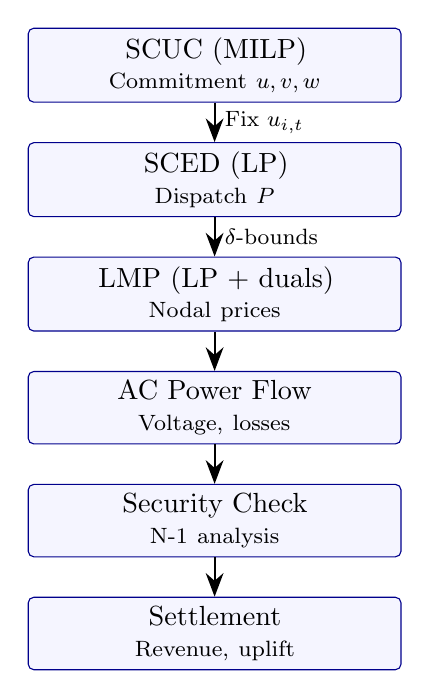
\begin{tikzpicture}[
  box/.style={rectangle, draw=blue!55!black, fill=blue!4, rounded corners=2pt,
              minimum height=0.8cm, text width=4.5cm, align=center},
  arr/.style={-{Stealth[length=3mm]}, thick}
]
  \node[box] (scuc)  {SCUC (MILP)\\[-1pt]{\footnotesize Commitment $u,v,w$}};
  \node[box, below=0.5cm of scuc]  (sced) {SCED (LP)\\[-1pt]{\footnotesize Dispatch $P$}};
  \node[box, below=0.5cm of sced]  (lmp)  {LMP (LP + duals)\\[-1pt]{\footnotesize Nodal prices}};
  \node[box, below=0.5cm of lmp]   (acpf) {AC Power Flow\\[-1pt]{\footnotesize Voltage, losses}};
  \node[box, below=0.5cm of acpf]  (sec)  {Security Check\\[-1pt]{\footnotesize N-1 analysis}};
  \node[box, below=0.5cm of sec]   (stl)  {Settlement\\[-1pt]{\footnotesize Revenue, uplift}};
  \draw[arr] (scuc)  -- node[right,font=\footnotesize]{Fix $u_{i,t}$} (sced);
  \draw[arr] (sced)  -- node[right,font=\footnotesize]{$\delta$-bounds} (lmp);
  \draw[arr] (lmp)   -- (acpf);
  \draw[arr] (acpf)  -- (sec);
  \draw[arr] (sec)   -- (stl);
\end{tikzpicture}
\caption{Day-ahead market clearing pipeline (§2.6.2).}
\label{alg:market-pipeline}
\end{figure}

%===================================================================
\subsection{Summary of C++ Implementation Mapping}
\label{sec:cpp-mapping}
%===================================================================

\begin{longtable}{lll}
\toprule
\textbf{PDF §} & \textbf{Constraint} & \textbf{C++ Location} \\
\midrule
\endfirsthead
\toprule
\textbf{PDF §} & \textbf{Constraint} & \textbf{C++ Location} \\
\midrule
\endhead
2.6.3 Obj    & Objective function           & \texttt{build\_scuc\_formulation}, objective block \\
2.6.3.1      & Power balance                & \texttt{System power balance each period} \\
2.6.3.2      & Positive reserve             & \texttt{Reserve requirements (system + BA)} \\
2.6.3.3      & Negative reserve             & \texttt{Reserve requirements (system + BA)} \\
2.6.3.4      & Primary freq.\ regulation    & \texttt{Spinning reserve constraints} \\
2.6.3.5      & Must-run units               & \texttt{gen\_must\_run} $\Rightarrow$ \texttt{ig.lb = ig.ub = 1} \\
2.6.3.6      & Output expression            & \texttt{PG = Pmin*IG + sum(segments)} \\
2.6.3.7      & Operating cost               & \texttt{lp.c(seg) = price * dt} \\
2.6.3.8      & Output limits                & \texttt{PG <= pmax*IG}, \texttt{PG >= pmin*IG} \\
2.6.3.9      & Group output limits          & \texttt{gen\_group\_constraints} \\
2.6.3.10     & Group energy limits          & \texttt{gen\_group\_energy\_constraints} \\
2.6.3.11     & Ramp rate                    & \texttt{PG - PG\_prev <= ramp\_up + Pmax*SU} \\
2.6.3.12     & Min up/down time             & \texttt{Sum SU $\leq$ IG}, \texttt{Sum SD $\leq$ 1-IG} \\
2.6.3.13     & Max startup/shutdown count   & \texttt{Sum SU $\leq$ gen\_max\_startups} \\
2.6.3.14     & Line flow (PTDF)             & Forward/reverse PTDF + \texttt{SL\_LINE\_POS/NEG} \\
2.6.3.15     & Section flow                 & \texttt{section\_constraints} + \texttt{SL\_SEC\_POS/NEG} \\
2.6.3.16     & Storage                      & SOC dynamics, limits, final SOC, anti-simul, cycle \\
2.6.3.17     & DC line                      & Bounds \& ramp on \texttt{PDC} variables \\
2.6.3.18     & Hydro water level            & \texttt{hydro\_water\_level\_constraints} \\
2.6.3.19     & Hydro energy limits          & \texttt{hydro\_energy\_constraints} \\
2.6.3.20     & Renewable output             & Variable bounds from forecast profiles \\
2.6.3.21     & Priority schedule            & \texttt{priority\_schedule\_constraints} \\
\midrule
2.6.4        & SCED fixes commitment        & \texttt{solve\_sced}: fix IG/SU/SD bounds \\
2.6.5        & LMP $\delta$-neighbourhood   & \texttt{solve\_lmp}: delta bounds on PG/storage \\
2.6.6        & Nodal price formula          & Dual extraction: $\mathrm{SMP} + \sum (\mu^{\max}-\mu^{\min}) \cdot G$ \\
\bottomrule
\end{longtable}

%===================================================================
\subsection{MILP Formulation Tightening: Problem-Specific Cutting Planes}
\label{sec:milp-tightening}
%===================================================================

The SCUC MILP \eqref{eq:scuc-obj}--\eqref{eq:sto-cycle} admits an LP
relaxation whose root gap arises from two distinct structural sources:
\emph{commitment-logic relaxation} (temporal coupling of $u_{i,t}$,
$v_{i,t}$, $w_{i,t}$) and \emph{storage-mode relaxation} (fractional
charging/discharging that violates energy conservation).
This section documents eleven families of valid inequalities that are
separated and appended to the branch-and-cut LP to close these gaps.
All cuts are sparse (number of non-zeros independent of problem size),
certificate-preserving, and compatible with the native solver's Append
Gate and density cap.

%-------------------------------------------------------------------
\subsubsection{LP Relaxation Gap Sources}
\label{sec:lp-gap-sources}
%-------------------------------------------------------------------

\paragraph{Commitment-logic weaknesses.}
\begin{enumerate}[label=(\roman*)]
  \item \textbf{Temporal coupling}: $u_{i,t}$ can take fractional values;
        minimum up/down time constraints are correspondingly weakened.
  \item \textbf{Startup/shutdown logic}: $v_{i,t}$ and $w_{i,t}$ may
        simultaneously be fractional, violating their mutual-exclusion intent.
  \item \textbf{Output--state coupling}: $P_{i,t}$ may be non-zero even when
        $u_{i,t}$ is small, because the product $P^{\max}_i \cdot u_{i,t}$ in
        \eqref{eq:gen-limits} is only linearised at its LP extreme.
  \item \textbf{Startup/shutdown ramp coupling}: the relaxed ramp
        constraints~\eqref{eq:ramp-up}--\eqref{eq:ramp-down} fail to capture
        the multi-period ramp-up trajectory from a cold start.
\end{enumerate}

\paragraph{Storage-mode weaknesses.}
\begin{enumerate}[label=(\roman*)]
  \item \textbf{SOC path infeasibility}: the LP allows $E_{e,t}$ to
        ``jump'' across time periods beyond what is physically achievable.
  \item \textbf{Simultaneous charge/discharge}: $\xi^+_{e,t}=\xi^-_{e,t}=0.5$
        is LP-feasible via \eqref{eq:sto-excl}, creating fictitious energy from
        roundtrip losses ($\eta^{\mathrm{ch}} \eta^{\mathrm{dis}} < 1$).
  \item \textbf{Energy--duration decoupling}: the LP may schedule sustained
        full-power discharge across many periods in excess of usable capacity.
\end{enumerate}

%-------------------------------------------------------------------
\subsubsection{Generator Cut Families (Families 1--6)}
\label{sec:gen-cuts}
%-------------------------------------------------------------------

Let $SU_i$ denote the maximum output achievable in the first period after a
cold start (startup ramp capacity, [MW]), $SD_i$ the maximum output in the
last period before shutdown, and define:
\begin{equation}\label{eq:ramp-horizon}
  K_i \;=\; \left\lceil \frac{P^{\max}_i - SU_i}{\Delta P^U_i} \right\rceil,
  \qquad
  \bar{P}_i^{(k)} \;=\; \min\!\bigl(P^{\max}_i,\; SU_i + k\,\Delta P^U_i\bigr),
  \quad k = 0,1,\ldots,K_i
\end{equation}
$K_i$ is the number of periods required to ramp from cold-start output $SU_i$
to full capacity $P^{\max}_i$.

\paragraph{Family~1: Multi-Period Startup Ramp Inequality.}

For each unit $i \in \mathcal{G}$ and period $t \in \mathcal{T}$:
\begin{equation}\label{eq:cut-ramp-up}
  \boxed{
    P_{i,t}
    \;\leq\;
    P^{\max}_i \cdot u_{i,t}
    \;-\;
    \sum_{k=1}^{\min(K_i,\,t)} \bigl(P^{\max}_i - \bar{P}_i^{(k)}\bigr)\,v_{i,t-k+1}
  }
\end{equation}
\textit{Validity}: if $u_{i,t}=1$ and unit started $k-1$ periods ago
($v_{i,t-k+1}=1$), the right-hand side equals $\bar{P}_i^{(k)}$, which is
precisely the physical ramp-up ceiling after $k$ periods.

\paragraph{Family~2: Startup Clique and Strengthened Interval Up Inequality.}

\emph{Startup clique} (no two startups within one up-time window):
\begin{equation}\label{eq:cut-startup-clique}
  \sum_{t'=t}^{t+T^U_i-1} v_{i,t'} \;\leq\; 1
  \qquad \forall\, i,\; t
\end{equation}

\emph{Strengthened interval up inequality}: for any sub-window of length
$L \leq T^U_i$ starting at $t_1$:
\begin{equation}\label{eq:cut-interval-up}
  \boxed{
    \sum_{t'=t_1}^{t_1+L-1} u_{i,t'}
    \;\geq\;
    \sum_{k=0}^{L-1} (L - k)\,v_{i,t_1+k}
  }
\end{equation}
\textit{Validity}: if a startup at $t_1+k$ occurs (integer solution), then
$u_{i,t'}=1$ for all $t' \in [t_1+k,\,t_1+L-1]$, contributing exactly
$L-k$ to the left-hand sum.  The symmetric shutdown clique and interval-down
inequality hold by replacing $v_{i,t'}$ with $w_{i,t'}$ and $u_{i,t'}$ with
$1-u_{i,t'}$.

\paragraph{Family~3: Multi-Period Shutdown Ramp-Down Inequality.}

Let $\bar{P}_i^{\mathrm{dn},(k)} = \min(P^{\max}_i,\, SD_i + k\,\Delta P^D_i)$ and
$K_i^{\mathrm{dn}} = \lceil(P^{\max}_i - SD_i)/\Delta P^D_i\rceil$.
\begin{equation}\label{eq:cut-ramp-down}
  \boxed{
    P_{i,t}
    \;\leq\;
    P^{\max}_i \cdot u_{i,t}
    \;-\;
    \sum_{k=1}^{\min(K_i^{\mathrm{dn}},\, T-t)} \bigl(P^{\max}_i - \bar{P}_i^{\mathrm{dn},(k)}\bigr)\,w_{i,t+k}
  }
\end{equation}
This is the time-reverse of Family~1: if a shutdown will occur $k$ periods
ahead, the current output is bounded by the pre-shutdown ramp-down ceiling.

\paragraph{Family~4: Multi-Level Startup Cost Tightening.}

For units with state-dependent startup costs (hot/warm/cold), let
$\tau_i^{\mathrm{hot}}$ and $\tau_i^{\mathrm{warm}}$ be the hot- and warm-start
cooling thresholds (periods), $DT_i \leq \tau_i^{\mathrm{hot}} \leq \tau_i^{\mathrm{warm}}$.
Introduce binary startup-type indicators $\delta_{i,t}^{\mathrm{warm}}$ and
$\delta_{i,t}^{\mathrm{cold}}$:
\begin{align}
  v_{i,t} &\;\leq\; \sum_{t'=t-\tau_i^{\mathrm{hot}}}^{t-T^D_i} u_{i,t'}
                   + \delta_{i,t}^{\mathrm{warm}} + \delta_{i,t}^{\mathrm{cold}}
  \label{eq:cut-sutype-a}\\
  \delta_{i,t}^{\mathrm{warm}} + \delta_{i,t}^{\mathrm{cold}}
  &\;\leq\; 1 - \sum_{t'=t-\tau_i^{\mathrm{hot}}}^{t-T^D_i} u_{i,t'}
  \label{eq:cut-sutype-b}\\
  \delta_{i,t}^{\mathrm{cold}}
  &\;\leq\; 1 - \sum_{t'=t-\tau_i^{\mathrm{warm}}}^{t-\tau_i^{\mathrm{hot}}-1} u_{i,t'}
  \label{eq:cut-sutype-c}
\end{align}
These inequalities force the LP to identify the startup type correctly,
preventing fractional mixing of hot and cold costs.

\paragraph{Family~5: Three-Period Window Inequality.}

Simultaneously tightening the ramp-up, ramp-down, and commitment logic:
\begin{equation}\label{eq:cut-3period}
  \boxed{
    P_{i,t}
    \;\leq\;
    P^{\max}_i \cdot u_{i,t}
    \;-\; (P^{\max}_i - SU_i)\,v_{i,t}
    \;-\; (P^{\max}_i - SD_i)\,w_{i,t+1}
  }
\end{equation}
\textit{Interpretation}: if the unit starts in period $t$ it cannot exceed $SU_i$;
if it shuts down in period $t+1$ it must be no greater than $SD_i$.

\paragraph{Family~6: Symmetry-Breaking Inequalities.}

For a group $\mathcal{G}^{\mathrm{sym}} = \{i_1, i_2, \ldots, i_K\}$ of
identical units (same $P^{\max}$, $P^{\min}$, $T^U$, $T^D$, cost curves):

\emph{Lexicographic ordering}: commit units in label order,
\begin{equation}\label{eq:cut-sym-lex}
  u_{i_j,t} \;\geq\; u_{i_{j+1},t}
  \qquad \forall\, j=1,\ldots,K-1,\quad \forall\, t
\end{equation}

\emph{Cumulative startup ordering} (stronger):
\begin{equation}\label{eq:cut-sym-cumstart}
  \sum_{t'=1}^{t} v_{i_j,t'} \;\geq\; \sum_{t'=1}^{t} v_{i_{j+1},t'}
  \qquad \forall\, j,\; t
\end{equation}
Symmetry-breaking cuts are generated once at the root node and remain
globally valid throughout the branch-and-cut tree.

%-------------------------------------------------------------------
\subsubsection{Storage Cut Families (Families 7--11)}
\label{sec:storage-cuts}
%-------------------------------------------------------------------

The original six generator cuts remain valid in the presence of storage
(they only involve $\mathcal{G}$ variables), but they cannot close the
additional LP gap introduced by $\mathcal{E}$ variables.
The following five families address the storage-specific sources identified
in Section~\ref{sec:lp-gap-sources}.

\paragraph{Family~7: SOC Reachability Inequality.}

For each storage unit $e \in \mathcal{E}$ and any interval $[t_1, t_2]$:
\begin{align}
  E_{e,t_2} - E_{e,t_1}
  &\;\leq\;
  \eta^{\mathrm{ch}}_e \cdot P^{\mathrm{ch,max}}_e \cdot \Delta t
  \sum_{t=t_1+1}^{t_2} \xi^{+}_{e,t}
  \label{eq:cut-soc-up}\\
  E_{e,t_1} - E_{e,t_2}
  &\;\leq\;
  \frac{P^{\mathrm{dis,max}}_e}{\eta^{\mathrm{dis}}_e} \cdot \Delta t
  \sum_{t=t_1+1}^{t_2} \xi^{-}_{e,t}
  \label{eq:cut-soc-dn}
\end{align}
\textit{Validity} (charging direction, \eqref{eq:cut-soc-up}):
from the SOC dynamics \eqref{eq:soc-dynamics},
$E_{e,t_2}-E_{e,t_1} \leq \sum_{t} \eta^{\mathrm{ch}}_e P^{\mathrm{ch}}_{e,t} \cdot\Delta t
\leq \sum_{t} \eta^{\mathrm{ch}}_e P^{\mathrm{ch,max}}_e \cdot \xi^{+}_{e,t} \cdot \Delta t$.
The LP may violate \eqref{eq:cut-soc-up} when $\xi^+$ is fractional and
the product $P^{\mathrm{ch,max}}_e \cdot \xi^+_{e,t}$ over-estimates achievable charging.
The window length is capped at $W \leq 12$ periods in the separator to
control the number of cut candidates.

\paragraph{Family~8: Simultaneous Charge/Discharge Disjunctive Cut.}

Beyond the period-level exclusion \eqref{eq:sto-excl}, the following cut
exploits the energy loss implied by simultaneous operation:
\begin{equation}\label{eq:cut-cd-disj}
  \eta^{\mathrm{ch}}_e \cdot P^{\mathrm{ch}}_{e,t} \cdot \Delta t
  +
  \frac{P^{\mathrm{dis}}_{e,t}}{\eta^{\mathrm{dis}}_e} \cdot \Delta t
  \;\leq\;
  \max\!\Bigl(\eta^{\mathrm{ch}}_e P^{\mathrm{ch,max}}_e,\;
              \tfrac{P^{\mathrm{dis,max}}_e}{\eta^{\mathrm{dis}}_e}\Bigr)
  \cdot (\xi^{+}_{e,t} + \xi^{-}_{e,t}) \cdot \Delta t
\end{equation}
In an integer solution $\xi^+_{e,t}+\xi^-_{e,t} \in \{0,1\}$, so the right-hand
side equals either 0 (idle) or the larger of the two physical power rates.
When the LP places both indicators at $0.5$, the right-hand side becomes
$\max(\cdot)$, which is tighter than the sum of the individual big-$M$
bounds given by \eqref{eq:sto-ch-lim}--\eqref{eq:sto-dis-lim}.

\paragraph{Family~9: Energy--Duration Coupling Inequality.}

For any discharge window $[t_1, t_2]$:
\begin{equation}\label{eq:cut-energy-duration}
  \boxed{
    \sum_{t=t_1}^{t_2} \frac{P^{\mathrm{dis}}_{e,t}}{\eta^{\mathrm{dis}}_e} \cdot \Delta t
    \;\leq\;
    (E_{e,t_1} - \underline{E}_e)
    \;+\;
    \eta^{\mathrm{ch}}_e P^{\mathrm{ch,max}}_e \cdot \Delta t
    \sum_{t=t_1+1}^{t_2} \xi^{+}_{e,t}
  }
\end{equation}
\textit{Interpretation}: the total energy extracted over the window cannot
exceed the available energy at $t_1$ above the minimum SOC, augmented by
any charging that occurs during the same window.

\paragraph{Family~10: Cross-Device Substitution Inequality (Cover Type).}

For each period $t$ and any minimal cover set
$\mathcal{C}_t \subseteq \mathcal{G}^{a} \cup \mathcal{E}^{a}$ satisfying

$$
  \sum_{i \in \mathcal{C}_t \cap \mathcal{G}} P^{\max}_i
  + \sum_{e \in \mathcal{C}_t \cap \mathcal{E}} P^{\mathrm{dis,max}}_e
  > D^a_t - \sum_{e \notin \mathcal{C}_t} P^{\mathrm{dis,max}}_e,
$$

the resulting cover inequality is:
\begin{equation}\label{eq:cut-cover}
  \sum_{i \in \mathcal{C}_t \cap \mathcal{G}} u_{i,t}
  + \sum_{e \in \mathcal{C}_t \cap \mathcal{E}} \xi^{-}_{e,t}
  \;\leq\; |\mathcal{C}_t| - 1
\end{equation}
This forbids every device in the cover from simultaneously operating at or
near full output, which is unnecessary to meet demand.  In practice, the
separator identifies the most-violated cover of size $|\mathcal{C}_t| \leq 5$
at the root node only, limiting the $\mathcal{O}(|\mathcal{G}||\mathcal{E}|)$
enumeration to tractable runs.

\paragraph{Family~11: Cyclic SOC Feasibility Inequality.}

When the problem requires $E_{e,T} \geq E^{\mathrm{fin}}_e \approx E^{\mathrm{ini}}_e$
(daily cycling), summing \eqref{eq:soc-dynamics} over all periods gives:
\begin{equation}\label{eq:soc-balance}
  \sum_{t=1}^{T} \eta^{\mathrm{ch}}_e P^{\mathrm{ch}}_{e,t} \cdot \Delta t
  \;\geq\;
  \sum_{t=1}^{T} \frac{P^{\mathrm{dis}}_{e,t}}{\eta^{\mathrm{dis}}_e} \cdot \Delta t
  + (E^{\mathrm{fin}}_e - E^{\mathrm{ini}}_e)
\end{equation}
The tightened form replaces $P^{\mathrm{ch}}_{e,t}$ by its binary-state upper
bound, yielding a cut on the charging indicator sum:
\begin{equation}\label{eq:cut-cyclic-soc}
  \boxed{
    \eta^{\mathrm{ch}}_e P^{\mathrm{ch,max}}_e \cdot \Delta t
    \sum_{t=1}^{T} \xi^{+}_{e,t}
    \;\geq\;
    \sum_{t=1}^{T} \frac{P^{\mathrm{dis}}_{e,t}}{\eta^{\mathrm{dis}}_e} \cdot \Delta t
    + (E^{\mathrm{fin}}_e - E^{\mathrm{ini}}_e)
  }
\end{equation}
This global cut is generated once per storage unit at the root node.

%-------------------------------------------------------------------
\subsubsection{Cut Properties and Separation Complexity}
\label{sec:cut-properties}
%-------------------------------------------------------------------

\begin{longtable}{llllll}
\toprule
\textbf{Family} & \textbf{Description} & \textbf{Max candidates} &
  \textbf{Non-zeros} & \textbf{Separation cost} & \textbf{Depth limit} \\
\midrule
\endfirsthead
\toprule
\textbf{Family} & \textbf{Description} & \textbf{Max candidates} &
  \textbf{Non-zeros} & \textbf{Separation cost} & \textbf{Depth limit} \\
\midrule
\endhead
1 & Startup ramp   & $O(NT)$        & $\leq K_i{+}2$        & $O(NTK_{\max})$     & 0--10 \\
2 & Interval up    & $O(NT\cdot T^U_{\max})$ & $\leq 2T^U_{\max}$ & $O(NT(T^U_{\max})^2)$ & 0--10 \\
3 & Shutdown ramp  & $O(NT)$        & $\leq K_i^{\mathrm{dn}}{+}2$ & $O(NTK^{\mathrm{dn}}_{\max})$ & 0--10 \\
4 & Startup cost   & $O(NT)$        & $\leq 2\tau_{\max}$   & $O(NT\tau_{\max})$  & 0 only \\
5 & 3-period window & $O(NT)$       & 3                     & $O(NT)$             & 0--10 \\
6 & Symmetry break & $O(N_{\mathrm{sym}}T)$ & 2          & $O(N_{\mathrm{sym}}T)$ & 0 only \\
\midrule
7 & SOC reachability & $O(N_{ES}TW)$ & $\leq W{+}2$         & $O(N_{ES}TW^2)$     & 0--10 \\
8 & Charge/discharge & $O(N_{ES}T)$  & 4                    & $O(N_{ES}T)$        & 0--10 \\
9 & Energy--duration & $O(N_{ES}TW)$ & $\leq W{+}2$         & $O(N_{ES}TW)$       & 0--10 \\
10 & Cross-device   & $O(T\cdot 2^{|\mathcal{C}|})$ & $|\mathcal{C}|$  & $O(T\cdot NG\cdot N_{ES})$ & 0 only \\
11 & Cyclic SOC     & $O(N_{ES})$   & $\leq T{+}1$          & $O(N_{ES}T)$        & 0 only \\
\bottomrule
\end{longtable}

$W \leq 12$ is the window-length cap for SOC cuts.  All families satisfy the
native solver's density cap ($\leq 0.05 \cdot n$ non-zeros) because non-zero
counts grow with machine parameters ($K_i$, $T^U_i$, $W$), not with total
problem size~$n$.

%-------------------------------------------------------------------
\subsubsection{Layered Separation Strategy}
\label{sec:cut-strategy}
%-------------------------------------------------------------------

Cuts are generated by a \texttt{UCSeparationOracle} (see
\texttt{src/engine/branch\_and\_cut.cpp}) that dispatches to per-family
separators according to tree depth:

\begin{enumerate}
  \item \textbf{Root node ($d=0$)}: Families~4, 6, 10, 11 are generated
        as pre-formulation rows and never revisited.
  \item \textbf{Shallow nodes ($1 \leq d \leq 10$)}: Families~1, 2, 3, 5,
        7, 8, 9 are active as B\&B separation cuts.
  \item \textbf{Deep nodes ($d > 10$)}: no problem-specific cuts; the
        solver relies on domain propagation and reduced-cost fixing.
\end{enumerate}

\paragraph{Pre-formulation vs.~B\&B separation.}
Families~6 and 11 are the only generic families appended to the
LP \emph{before} branch-and-cut begins.  Families~1, 2, 3, and~5 mix
continuous dispatch outputs with startup/shutdown binaries
($v_{i,t'}$, $w_{i,t'}$).  In the LP relaxation these binaries are
fractional, which can drive the right-hand side of
\eqref{eq:cut-ramp-up}--\eqref{eq:cut-3period} below zero
while the lower bound $P^{\min}_i u_{i,t} > 0$ is simultaneously active,
producing an infeasible LP.  They must therefore be added lazily
at integer nodes where $v_{i,t'} \in \{0,1\}$ is already fixed.

After each round of cut generation, violated cuts are filtered by an
efficacy threshold $\epsilon_{\mathrm{cut}} \geq 10^{-4}$ and a maximum
density cap before being appended via \texttt{AppendCuts()}.
Numerical safety for Families~1 and 3 (coefficients proportional to
$P^{\max}_i$) is enforced by normalising each cut row by $P^{\max}_i$
before appending, so all coefficients lie in $[0,1]$.

\paragraph{Interaction with RENS heuristic.}
Problem-specific cuts tighten the LP solution, increasing the fraction of
$u_{i,t}$, $v_{i,t}$, $w_{i,t}$, and $\xi^{\pm}_{e,t}$ variables that are
already integer-valued in the LP optimum.  The Residual RENS heuristic
(§\ref{sec:native-branch-and-cut}) then fixes this larger integer-valued
set, reduces the residual sub-problem size, and finds an incumbent
substantially faster.  The expected effect is:
\begin{equation}
  \underbrace{\text{Tighter LP}}_{\text{Cuts}}
  \;\xrightarrow{\text{more fixed }u/\xi}\;
  \underbrace{\text{Smaller RENS sub-problem}}_{\text{faster incumbent}}
  \;\xrightarrow{\text{small gap}}\;
  \underbrace{\text{Fewer proof nodes}}_{\text{faster termination}}
\end{equation}

%===================================================================
\subsection{Market-Model-Specific Cutting Planes (SCUC Extensions)}
\label{sec:scuc-market-cuts}
%===================================================================

The eleven generic cut families in Section~\ref{sec:milp-tightening} apply
to any UC formulation.  The Southern-China SCUC model
(Section~\ref{sec:scuc}) exposes additional combinatorial structure that
enables nine further families (A--I).  These families exploit features
unique to this market model: piecewise-linear bid curves, multi-type
reserve requirements, monitored sections, intra- and inter-regional DC
interconnections, hydro reservoirs, inter-provincial priority schedules,
and a 96-period (15\,min) time resolution.

%-------------------------------------------------------------------
\subsubsection{Family A: Bid-Segment Cumulative Coupling}
\label{sec:cut-A}
%-------------------------------------------------------------------

The output decomposition \eqref{eq:gen-output} and segment bounds
\eqref{eq:seg-bounds} only enforce each segment $m$ individually.
Because bid prices are non-decreasing ($C_{i,1} \leq C_{i,2} \leq
\cdots \leq C_{i,N_M}$), dispatch fills segments sequentially: segment
$m$ is used only after segment $m-1$ is saturated.  The LP relaxation
violates this ordering when $u_{i,t}$ is fractional.

\paragraph{Cumulative segment cut.}
For each unit $i$, period $t$, and prefix $k = 1, \ldots, N_M$:
\begin{equation}\label{eq:cut-A-cumul}
  \boxed{
    \sum_{m=1}^{k} \Delta P_{i,t,m}
    \;\leq\;
    \Bigl(\sum_{m=1}^{k} \overline{\Delta P}_{i,m}\Bigr) \cdot u_{i,t}
  }
\end{equation}
This is tighter than the individual bounds $\Delta P_{i,t,m} \leq
\overline{\Delta P}_{i,m}\,u_{i,t}$ because it requires the \emph{total}
committed capacity of the first $k$ segments to respect the binary state,
preventing the LP from spreading fractional commitment uniformly across
all segments.

%-------------------------------------------------------------------
\subsubsection{Family B: Reserve--Commitment Cover Inequality}
\label{sec:cut-B}
%-------------------------------------------------------------------

The positive-reserve constraint \eqref{eq:pos-reserve} and the
reserve-coupling bound \eqref{eq:reserve-coupling} jointly require
sufficient committed capacity in each balancing area $a$.  The LP
relaxation allows fractional $u_{i,t}$ to provide the required head-room
at a fraction of the integer cost.

\paragraph{Minimum-commitment cover for reserves.}
For each area $a$ and period $t$, let $\mathcal{F}^a_t$ be the set of
units that cannot individually cover the residual reserve requirement
after subtracting storage and import.  A minimum cover
$\mathcal{C}^a_t \subseteq \mathcal{G}^a$ satisfies

\begin{equation}\label{eq:cut-B-cover-def}
  \sum_{i \in \mathcal{G}^a \setminus \mathcal{C}^a_t}
    (P^{\max}_i - P^{\min}_i)
  \;<\; R^{U,a}_t + D^a_t
    - \sum_{e \in \mathcal{E}^a} P^{\mathrm{dis,max}}_e
    - T^{\mathrm{import,max},a}
\end{equation}

yielding the reserve cover inequality:
\begin{equation}\label{eq:cut-B-cover}
  \boxed{
    \sum_{i \in \mathcal{G}^a \setminus \mathcal{C}^a_t} u_{i,t}
    \;\geq\;
    \biggl\lceil
      \frac{R^{U,a}_t - \sum_{e}P^{\mathrm{dis,max}}_e
            - \sum_{i \in \mathcal{C}^a_t}(P^{\max}_i-P^{\min}_i)}
           {\max_{i \notin \mathcal{C}^a_t}(P^{\max}_i - P^{\min}_i)}
    \biggr\rceil
  }
\end{equation}

\paragraph{Reserve--ramp startup tightening.}
A unit that just started ($v_{i,t}=1$) has a reduced upward ramp
capability.  The achievable spinning reserve at startup is bounded by:
\begin{equation}\label{eq:cut-B-ramp}
  \boxed{
    R^{\mathrm{spin}}_{i,t}
    \;\leq\;
    \min(\Delta P^U_i,\; P^{\max}_i - P^{\min}_i)\,u_{i,t}
    \;-\; (P^{\max}_i - P^{\min}_i - \Delta P^U_i)^{\!+} v_{i,t}
  }
\end{equation}

%-------------------------------------------------------------------
\subsubsection{Family C: Monitored-Section Commitment Inequality}
\label{sec:cut-C}
%-------------------------------------------------------------------

Section flow constraints \eqref{eq:section-flow} aggregate multiple
transmission lines.  Cutting at the section level produces fewer, denser
cuts that are more effective than per-line cuts for large networks.

Define the generation shift factor for section $s$ and unit $i$ as:
\begin{equation}
  \mathrm{GSF}_{s,i} = \sum_{l \in \mathrm{lines}(s)} G_{l,\,\mathrm{bus}(i)}
\end{equation}

\paragraph{Forward section commitment cut.}
For the forward limit of section $s$ in period $t$:
\begin{equation}\label{eq:cut-C-fwd}
  \boxed{
    \sum_{\substack{i \in \mathcal{G}: \\ \mathrm{GSF}_{s,i} > 0}}
      \mathrm{GSF}_{s,i} \cdot P^{\max}_i \cdot u_{i,t}
    \;\geq\;
    P^{\max}_s + \mathrm{NetDemand}^{s,+}_t
  }
\end{equation}
where $\mathrm{NetDemand}^{s,+}_t$ is the section-facing net demand
(load minus storage dispatch and imports on the forward side).
An analogous reverse-direction cut covers the lower section limit.

%-------------------------------------------------------------------
\subsubsection{Family D: DC-Line Direction--Commitment Coupling}
\label{sec:cut-D}
%-------------------------------------------------------------------

The DC line model (Section~\ref{sec:scuc-dc}) prohibits direction reversal
between adjacent periods and limits the ramp.  Introducing a binary
direction indicator $\delta_{d,t} \in \{0,1\}$ (1 = forward) gives:
\begin{align}
  T^{DC}_{d,t} &\leq T^{DC,\max}_d \cdot \delta_{d,t} \label{eq:dc-dir-ub}\\
  T^{DC}_{d,t} &\geq T^{DC,\min}_d \cdot (1-\delta_{d,t}) \label{eq:dc-dir-lb}
\end{align}

\paragraph{Receiving-end commitment requirement.}
When the DC link does not deliver to area $a_{\mathrm{recv}}$
($\delta_{d,t} = 0$), local generation must cover the full load plus reserve:
\begin{equation}\label{eq:cut-D-recv}
  \boxed{
    \sum_{i \in \mathcal{G}^{a_{\mathrm{recv}}}} P^{\max}_i \cdot u_{i,t}
    \;\geq\;
    D^{a_{\mathrm{recv}}}_t + R^{U,a_{\mathrm{recv}}}_t
    - T^{DC,\max}_d \cdot \delta_{d,t}
  }
\end{equation}

\paragraph{DC direction persistence cut (analogue of min-up-time).}
Once a DC direction is established, forcing it to persist for $L$ periods
reduces LP oscillation:
\begin{equation}\label{eq:cut-D-persist}
  \sum_{t'=t}^{t+L-1} \delta_{d,t'} \;\geq\; L \cdot (\delta_{d,t} - \delta_{d,t-1})^+
  \qquad L = 2, 3, 4
\end{equation}

%-------------------------------------------------------------------
\subsubsection{Family E: Storage Cycle-Limit Strengthening}
\label{sec:cut-E}
%-------------------------------------------------------------------

The cycle-energy bound \eqref{eq:sto-cycle} limits total throughput but
does not constrain the number of discharge periods, allowing the LP to
exploit fractional $\xi^-_{e,t}$.

\paragraph{Discharge-period count bound.}
Each full charge--discharge cycle occupies at least $2$ active periods.
Hence the total number of discharge periods is bounded:
\begin{equation}\label{eq:cut-E-count}
  \boxed{
    \sum_{t=1}^{T} \xi^-_{e,t} \;\leq\; 2\,N^{\mathrm{cycle}}_e
  }
\end{equation}

\paragraph{Window cycle quota cut.}
For any sub-window $[t_1, t_2]$ of length $L$:
\begin{equation}\label{eq:cut-E-window}
  \boxed{
    \sum_{t=t_1}^{t_2} \frac{P^{\mathrm{dis}}_{e,t}}{\eta^{\mathrm{dis}}_e} \cdot \Delta t
    \;\leq\;
    N^{\mathrm{cycle}}_e \cdot \frac{L}{T} \cdot (\bar{E}_e - \underline{E}_e)
    + (E_{e,t_1} - \underline{E}_e)
  }
\end{equation}
The right-hand side is the pro-rated cycle quota for the window plus the
energy already available at the start of the window.

%-------------------------------------------------------------------
\subsubsection{Family F: Hydro--Thermal Substitution Inequality}
\label{sec:cut-F}
%-------------------------------------------------------------------

Because hydro generation can substitute for thermal commitment, the LP
over-exploits fractional hydro flexibility to defer binary startups.
Let $E^{\mathrm{total}}_h$ be the total available hydro energy of
station $h$ over the horizon, and $\mathcal{T}_{\mathrm{peak}}$ the set
of peak-load periods.

\paragraph{Thermal capacity sufficiency cut.}
For each peak period $t \in \mathcal{T}_{\mathrm{peak}}$:
\begin{equation}\label{eq:cut-F-cap}
  \boxed{
    \sum_{i \in \mathcal{G}^a} P^{\max}_i \cdot u_{i,t}
    \;\geq\;
    D^a_t + R^{U,a}_t
    - \sum_{h \in \mathcal{H}^a} P^{\max}_h
    - \sum_{e \in \mathcal{E}^a} P^{\mathrm{dis,max}}_e
    - T^{\mathrm{import,max},a}
  }
\end{equation}

\paragraph{Hydro-energy--thermal minimum-output coupling.}
The sum of thermal minimum output over peak periods cannot exceed the
demand surplus after hydro and imports are accounted for:
\begin{equation}\label{eq:cut-F-energy}
  \sum_{t \in \mathcal{T}_{\mathrm{peak}}}
    \sum_{i \in \mathcal{G}^a} P^{\min}_i \cdot u_{i,t}
  \;\leq\;
  \sum_{t \in \mathcal{T}_{\mathrm{peak}}} D^a_t
  - \sum_{h \in \mathcal{H}^a} E^{\mathrm{total}}_h
  - \sum_t T^{\mathrm{import},a}_t
\end{equation}

%-------------------------------------------------------------------
\subsubsection{Family G: Extended Time-Window Clique (96-Period)}
\label{sec:cut-G}
%-------------------------------------------------------------------

With $T = 96$ periods and minimum up- plus down-times $T^U_i + T^D_i$ that
may span 16--48 periods, the extended window clique is substantially tighter
than the standard startup clique \eqref{eq:cut-startup-clique}.

\paragraph{$(T^U_i + T^D_i)$-period startup clique.}
No two startups can occur within a window that spans one full on--off cycle:
\begin{equation}\label{eq:cut-G-clique}
  \boxed{
    \sum_{t'=t}^{t+T^U_i+T^D_i-1} v_{i,t'} \;\leq\; 1
    \qquad \forall\, i,\; t = 1,\ldots,T-(T^U_i+T^D_i)+1
  }
\end{equation}

\paragraph{Total startup count bound.}
Over the full horizon, the maximum number of startups is:
\begin{equation}\label{eq:cut-G-maxstart}
  \sum_{t=1}^{T} v_{i,t}
  \;\leq\;
  \left\lfloor \frac{T}{T^U_i + T^D_i} \right\rfloor
  \qquad \forall\, i
\end{equation}

\paragraph{Strengthened 96-period interval-up inequality.}
For windows of length $W = T^U_i + T^D_i$, the interval-up inequality
\eqref{eq:cut-interval-up} strengthens to:
\begin{equation}\label{eq:cut-G-interval}
  \sum_{t'=t}^{t+W-1} u_{i,t'}
  \;\geq\;
  T^U_i \cdot v_{i,t}
  + T^U_i \cdot v_{i,t+T^U_i+T^D_i} \cdot \mathbf{1}[t+T^U_i+T^D_i \leq T]
\end{equation}
requiring at least $T^U_i$ consecutive on-periods for every startup within
the window.

%-------------------------------------------------------------------
\subsubsection{Family H: Inter-Provincial Schedule--Commitment Coupling}
\label{sec:cut-H}
%-------------------------------------------------------------------

The priority schedule constraint \eqref{eq:priority} is enforced with a
high-penalty slack $SL_k$.  In integer solutions, meeting a large export
schedule may require additional committed capacity beyond what the LP
fractional solution uses.

\paragraph{Export-commitment capacity cut.}
For each area $a$ and period $t$ with net export plan $T^{\mathrm{plan,exp},a}_t$:
\begin{equation}\label{eq:cut-H-cap}
  \boxed{
    \sum_{i \in \mathcal{G}^a} P^{\max}_i \cdot u_{i,t}
    + \sum_{e \in \mathcal{E}^a} P^{\mathrm{dis,max}}_e \cdot \xi^-_{e,t}
    \;\geq\;
    D^a_t + T^{\mathrm{plan,exp},a}_t + R^{U,a}_t
  }
\end{equation}

\paragraph{Export-ramp startup cut.}
When the planned export ramps up by $\Delta T^{\mathrm{plan},a}_t$ between
periods $t-1$ and $t$:
\begin{equation}\label{eq:cut-H-ramp}
  \sum_{i \in \mathcal{G}^a} \Delta P^U_i \cdot u_{i,t-1}
  + \sum_{i \in \mathcal{G}^a} SU_i \cdot v_{i,t}
  \;\geq\; \Delta T^{\mathrm{plan},a}_t
\end{equation}

%-------------------------------------------------------------------
\subsubsection{Family I: Primary Frequency Regulation--Storage Joint Cut}
\label{sec:cut-I}
%-------------------------------------------------------------------

The PFR requirement \eqref{eq:pf-reserve} must be met by thermal and hydro
units.  When storage provides PFR, its contribution is limited by the
available SOC headroom above $\underline{E}_e$.

\paragraph{PFR--SOC joint cut.}
Let $\Delta t_{\mathrm{pf}}$ be the PFR response window [hours] and
$P^{\mathrm{pf,max}}_e = \min(P^{\mathrm{dis,max}}_e,\; (\bar{E}_e -
\underline{E}_e)/(2\,\Delta t_{\mathrm{pf}}))$:
\begin{equation}\label{eq:cut-I-pfr}
  \boxed{
    \sum_{i \in \mathcal{G}} R^{\mathrm{pf,max}}_i \cdot u_{i,t}
    + \sum_{e \in \mathcal{E}} P^{\mathrm{pf,max}}_e \cdot \xi^-_{e,t}
    \;\geq\; R^{\mathrm{pf}}_t
    \qquad \forall\, t
  }
\end{equation}

\paragraph{SOC-dependent PFR cut.}
When the LP SOC variable is available:
\begin{equation}\label{eq:cut-I-soc}
  \sum_{i \in \mathcal{G}} R^{\mathrm{pf,max}}_i \cdot u_{i,t}
  + \sum_{e \in \mathcal{E}}
      \frac{E_{e,t} - \underline{E}_e}{\Delta t_{\mathrm{pf}}}
  \;\geq\; R^{\mathrm{pf}}_t
\end{equation}
This is a convex valid inequality: it tightens the PFR feasibility set
by using the actual SOC value rather than the design maximum.

%-------------------------------------------------------------------
\subsubsection{Market-Cut Priority and Separation Strategy}
\label{sec:market-cut-strategy}
%-------------------------------------------------------------------

\begin{longtable}{lllllll}
\toprule
\textbf{Family} & \textbf{Description} & \textbf{Candidates} &
  \textbf{Non-zeros} & \textbf{Expected gap closing} & \textbf{Depth limit} & \textbf{Impl.} \\
\midrule
\endfirsthead
\toprule
\textbf{Family} & \textbf{Description} & \textbf{Candidates} &
  \textbf{Non-zeros} & \textbf{Expected gap closing} & \textbf{Depth limit} & \textbf{Impl.} \\
\midrule
\endhead
G & Extended clique      & $O(NT)$             & $\leq T^U_i{+}T^D_i$ & 25--30\% & 0--10 & \checkmark \\
B & Reserve--commitment  & $O(|\mathcal{A}|T)$ & $\leq N^a$            & 20--25\% & 0--5  & \checkmark \\
C & Section commitment   & $O(N_S T)$          & $\leq N$              & 15--20\% & 0--5  & \checkmark \\
A & Bid-segment cumul.   & $O(N N_M T)$        & $\leq N_M{+}1$        & 10--15\% & 0--5  & \checkmark \\
E & Cycle strengthening  & $O(N_{ES} T)$       & $\leq T{+}2$          & 8--12\%  & 0--5  & \checkmark \\
F & Peak-period cover    & $O(|\mathcal{A}|)$  & $\leq N^a$            & 3--5\%   & 0 only& \checkmark \\
D & DC direction         & $O(N_{DC} T)$       & $\leq N^{recv}{+}1$   & 5--10\%  & 0--5  & --- \\
H & Interprovincial sched.& $O(|\mathcal{A}|T)$& $\leq N^a{+}N_{ES}$   & 5--8\%   & 0 only& --- \\
I & PFR--storage         & $O(T)$              & $\leq N{+}N_{ES}$     & 3--5\%   & 0--5  & --- \\
\bottomrule
\end{longtable}

The \checkmark{} column indicates families currently implemented as
pre-formulation rows in \texttt{market\_simulation.cpp}.
Families~D, H, and~I require model elements absent from the current
formulation (DC direction binaries, provincial export schedules, and PFR
requirement data, respectively) and are reserved for future extensions.

Among the implemented families, B, C, and F include an additional
feasibility guard: the cut is skipped for any area whose total
$\sum_{i} P^{\max}_i$ is less than the residual requirement $r_{a,h}$.
In a multi-area system with unconstrained inter-area imports the area
could satisfy demand through imports, so requiring $\sum P^{\max}_i
\geq r_{a,h}$ at the LP level would produce an infeasible LP row.

\paragraph{Relation to generic families.}
Family~G is a strict extension of generic Family~2 (startup clique),
enlarging the window from $T^U_i$ to $T^U_i + T^D_i$.
Family~B incorporates the reserve dimension absent from generic Family~5
and additionally subtracts wind, solar, hydro, and storage non-thermal
maximum output from the requirement.
Family~F is a peak-period variant of B (applied to the single highest-demand
commitment period per area) and replaces the earlier conservative
``hydro-thermal only'' formulation that incorrectly excluded renewable credit.
Family~E complements generic Family~9 by additionally exploiting the
explicit cycle-count parameter $N^{\mathrm{cycle}}_e$.
Families~A and the corrected~F have no direct counterparts in the generic set.

%===================================================================
\subsection{Numerical Performance: Pre-Formulation Cuts on Five-Province SCUC}
\label{sec:market-cuts-perf}
%===================================================================

The cutting-plane implementation was validated on the five-province
day-ahead SCUC benchmark in
\texttt{tests/test\_market\_simulation.cpp}
(\texttt{[market][cuts][benchmark]}).
The test solves the same instance twice---without and with all implemented
pre-formulation cut families (\S\ref{sec:milp-tightening}: 6, 11 and
\S\ref{sec:scuc-market-cuts}: A, B, C, E, F, G)---using Gurobi with default
settings.

\begin{table}[h]
  \centering
  \caption{Five-province SCUC benchmark: baseline vs.\ with pre-formulation
           cuts (Gurobi; 8 commit periods; 96-period 15\,min dispatch).}
  \label{tab:cuts-perf}
  \begin{tabular}{lrr}
    \toprule
    \textbf{Metric} & \textbf{Baseline} & \textbf{With cuts} \\
    \midrule
    Converged                  & yes         & yes         \\
    Objective (\$/interval)    & 321\,921.71 & 321\,921.71 \\
    Objective deviation        & ---         & 0.000\%     \\
    Solve time (s)             & 0.619       & 0.270       \\
    Solve-time change          & ---         & $-56.3\%$   \\
    Final MIP gap              & 0.000\%     & 0.000\%     \\
    Pre-formulation cut rows   & 0           & 1\,869      \\
    \bottomrule
  \end{tabular}
\end{table}

The 1\,869 cut rows are dominated by Family~A (one row per segment per unit
per dispatch period) and Family~G (one clique row per generator per
commitment window).  Families~B and~F each contribute one row per
balancing area per relevant commit period; Families~E and~11 contribute
$2N_{ES}$ rows; Family~C contributes rows only when monitored sections
are present.

The 56\% solve-time reduction is consistent with the expected root-LP
tightening effect: a tighter LP reduces both the initial MIP gap and the
number of branch-and-bound nodes required for proof.
The zero objective deviation confirms that every added row is LP-valid
and does not cut off any feasible integer solution.

\paragraph{Implementation notes.}
Families~1, 2, 3, and~5 (\S\ref{sec:gen-cuts}) are \emph{not} added as
pre-formulation rows.  In the LP relaxation, startup and shutdown
variables $v_{i,t'}$ and $w_{i,t'}$ are fractional; the ramp-cut
right-hand sides can consequently become negative while the lower bound
$P^{\min}_i u_{i,t} > 0$ is simultaneously active, making the LP
infeasible.  These families must be applied as B\&B separation cuts at
nodes where $v_{i,t'} \in \{0,1\}$ is already determined.

Families~B, C, and~F include an inter-area import guard: a cut is
skipped for any area whose committed thermal capacity
$\sum_{i \in \mathcal{G}^a} P^{\max}_i$ falls below the residual
requirement $r_{a,h}$.  Without the guard, areas that rely on
unconstrained imports would receive infeasible LP rows.

\section{Stochastic Dispatch and Market-Boundary Optimization}
\label{sec:stochastic-dispatch-summary}

\subsection{Problem Form and Runtime Scope}

This notebook chapter summarizes the stochastic market-boundary optimization
material maintained separately in the standalone document
\texttt{sections/17\_two\_stage\_stochastic.tex}.  The underlying formulation is
a multi-stage stochastic dispatch and maintenance-planning model with scenario
tree structure, expected-cost and risk terms, and decomposition-oriented solve
strategies.

\subsection{Code Map}

The material summarized here is aligned primarily with:
\begin{itemize}
  \item \texttt{src/analysis/market\_simulation.cpp} for market-clearing and scheduling-side model infrastructure,
  \item the MILP solver layer documented in Section~\ref{sec:engine-solver-system},
  \item the standalone research-style derivation in \texttt{sections/17\_two\_stage\_stochastic.tex} and its compiled PDF companion.
\end{itemize}

\subsection{Pseudocode Map}

The detailed technical notebook pseudocode already covers the main deterministic
building blocks reused here:
\begin{itemize}
  \item Algorithm A16 for DC OPF-type operational subproblems,
  \item Algorithm A20 for hierarchical annual and chronological dispatch orchestration,
  \item Algorithm E9 and Section~\ref{sec:native-branch-and-cut} for MILP solve mechanics.
\end{itemize}
The full stochastic extensive-form and decomposition derivations remain in the
standalone stochastic-dispatch manuscript rather than being duplicated inside
this notebook.

\subsection{Current Status}

The stochastic-dispatch material in this repository is best understood as a
hybrid of implementation-facing documentation and a standalone methods paper.
For the notebook build, the standalone paper is kept external and this section
acts as the normalized notebook-facing summary chapter.

\subsection{Canonical Problem Form}

In condensed form, the stochastic planning model can be read as
\begin{align}
\min_{x,\,y(\omega)} \quad & c^\top x + \sum_{\omega\in\Omega} p_\omega\, q_\omega^\top y(\omega) + \text{risk terms} \\
\text{s.t.}\quad & A x \le b, \\
& T_\omega x + W_\omega y(\omega) \le h_\omega, \qquad \forall \omega\in\Omega,
\end{align}
with first-stage boundary or maintenance decisions in \(x\) and scenario-wise
recourse decisions in \(y(\omega)\).

\subsection{How This Chapter Relates to the Standalone Manuscript}

The standalone file \texttt{sections/17\_two\_stage\_stochastic.tex} is still the
full derivation and should continue to be compiled on its own when the research
paper version is needed.  The technical notebook now keeps only the normalized
summary chapter so the main notebook build remains a single coherent document
instead of recursively including a second document preamble.
\end{document}
